\documentclass[twoside]{book}

% Packages required by doxygen
\usepackage{fixltx2e}
\usepackage{calc}
\usepackage{doxygen}
\usepackage[export]{adjustbox} % also loads graphicx
\usepackage{graphicx}
\usepackage[utf8]{inputenc}
\usepackage{makeidx}
\usepackage{multicol}
\usepackage{multirow}
\PassOptionsToPackage{warn}{textcomp}
\usepackage{textcomp}
\usepackage[nointegrals]{wasysym}
\usepackage[table]{xcolor}

% Font selection
\usepackage[T1]{fontenc}
\usepackage[scaled=.90]{helvet}
\usepackage{courier}
\usepackage{amssymb}
\usepackage{sectsty}
\renewcommand{\familydefault}{\sfdefault}
\allsectionsfont{%
  \fontseries{bc}\selectfont%
  \color{darkgray}%
}
\renewcommand{\DoxyLabelFont}{%
  \fontseries{bc}\selectfont%
  \color{darkgray}%
}
\newcommand{\+}{\discretionary{\mbox{\scriptsize$\hookleftarrow$}}{}{}}

% Page & text layout
\usepackage{geometry}
\geometry{%
  a4paper,%
  top=2.5cm,%
  bottom=2.5cm,%
  left=2.5cm,%
  right=2.5cm%
}
\tolerance=750
\hfuzz=15pt
\hbadness=750
\setlength{\emergencystretch}{15pt}
\setlength{\parindent}{0cm}
\setlength{\parskip}{3ex plus 2ex minus 2ex}
\makeatletter
\renewcommand{\paragraph}{%
  \@startsection{paragraph}{4}{0ex}{-1.0ex}{1.0ex}{%
    \normalfont\normalsize\bfseries\SS@parafont%
  }%
}
\renewcommand{\subparagraph}{%
  \@startsection{subparagraph}{5}{0ex}{-1.0ex}{1.0ex}{%
    \normalfont\normalsize\bfseries\SS@subparafont%
  }%
}
\makeatother

% Headers & footers
\usepackage{fancyhdr}
\pagestyle{fancyplain}
\fancyhead[LE]{\fancyplain{}{\bfseries\thepage}}
\fancyhead[CE]{\fancyplain{}{}}
\fancyhead[RE]{\fancyplain{}{\bfseries\leftmark}}
\fancyhead[LO]{\fancyplain{}{\bfseries\rightmark}}
\fancyhead[CO]{\fancyplain{}{}}
\fancyhead[RO]{\fancyplain{}{\bfseries\thepage}}
\fancyfoot[LE]{\fancyplain{}{}}
\fancyfoot[CE]{\fancyplain{}{}}
\fancyfoot[RE]{\fancyplain{}{\bfseries\scriptsize 制作者 Doxygen }}
\fancyfoot[LO]{\fancyplain{}{\bfseries\scriptsize 制作者 Doxygen }}
\fancyfoot[CO]{\fancyplain{}{}}
\fancyfoot[RO]{\fancyplain{}{}}
\renewcommand{\footrulewidth}{0.4pt}
\renewcommand{\chaptermark}[1]{%
  \markboth{#1}{}%
}
\renewcommand{\sectionmark}[1]{%
  \markright{\thesection\ #1}%
}

% Indices & bibliography
\usepackage{natbib}
\usepackage[titles]{tocloft}
\setcounter{tocdepth}{3}
\setcounter{secnumdepth}{5}
\makeindex

% Hyperlinks (required, but should be loaded last)
\usepackage{ifpdf}
\ifpdf
  \usepackage[pdftex,pagebackref=true]{hyperref}
\else
  \usepackage[ps2pdf,pagebackref=true]{hyperref}
\fi
\hypersetup{%
  colorlinks=true,%
  linkcolor=blue,%
  citecolor=blue,%
  unicode%
}

% Custom commands
\newcommand{\clearemptydoublepage}{%
  \newpage{\pagestyle{empty}\cleardoublepage}%
}

\usepackage{caption}
\captionsetup{labelsep=space,justification=centering,font={bf},singlelinecheck=off,skip=4pt,position=top}

%===== C O N T E N T S =====

\begin{document}

% Titlepage & ToC
\hypersetup{pageanchor=false,
             bookmarksnumbered=true,
             pdfencoding=unicode
            }
\pagenumbering{alph}
\begin{titlepage}
\vspace*{7cm}
\begin{center}%
{\Large Actiger \\[1ex]\large 1.\+1 }\\
\vspace*{1cm}
{\large 制作者 Doxygen 1.8.13}\\
\end{center}
\end{titlepage}
\clearemptydoublepage
\pagenumbering{roman}
\tableofcontents
\clearemptydoublepage
\pagenumbering{arabic}
\hypersetup{pageanchor=true}

%--- Begin generated contents ---
\chapter{继承关系索引}
\section{类继承关系}
此继承关系列表按字典顺序粗略的排序\+: \begin{DoxyCompactList}
\item \contentsline{section}{beeline\+\_\+t}{\pageref{structbeeline__t}}{}
\item \contentsline{section}{quadruped\+:\+:Body\+State\+Estimate}{\pageref{classquadruped_1_1BodyStateEstimate}}{}
\item \contentsline{section}{quadruped\+:\+:Body\+Trajectory}{\pageref{classquadruped_1_1BodyTrajectory}}{}
\item \contentsline{section}{quadruped\+:\+:Common}{\pageref{classquadruped_1_1Common}}{}
\item \contentsline{section}{quadruped\+:\+:Contact\+Spec}{\pageref{classquadruped_1_1ContactSpec}}{}
\begin{DoxyCompactList}
\item \contentsline{section}{quadruped\+:\+:Single\+Contact}{\pageref{classquadruped_1_1SingleContact}}{}
\end{DoxyCompactList}
\item \contentsline{section}{quadruped\+:\+:Dyn\+Model}{\pageref{classquadruped_1_1DynModel}}{}
\item \contentsline{section}{quadruped\+:\+:Dyn\+W\+BC}{\pageref{classquadruped_1_1DynWBC}}{}
\item \contentsline{section}{quadruped\+:\+:Endfoot\+Trajectory}{\pageref{classquadruped_1_1EndfootTrajectory}}{}
\item \contentsline{section}{quadruped\+:\+:F\+H\+\_\+constraints}{\pageref{classquadruped_1_1FH__constraints}}{}
\item \contentsline{section}{quadruped\+:\+:F\+H\+\_\+updata\+Info}{\pageref{classquadruped_1_1FH__updataInfo}}{}
\item \contentsline{section}{quadruped\+:\+:Floating\+Base\+Model}{\pageref{classquadruped_1_1FloatingBaseModel}}{}
\item \contentsline{section}{quadruped\+:\+:Foothold}{\pageref{classquadruped_1_1Foothold}}{}
\item \contentsline{section}{quadruped\+:\+:Gamepad}{\pageref{classquadruped_1_1Gamepad}}{}
\item \contentsline{section}{handle\+\_\+t}{\pageref{structhandle__t}}{}
\item \contentsline{section}{imu\+\_\+t}{\pageref{structimu__t}}{}
\item \contentsline{section}{Kalman\+Filter\+For\+VE}{\pageref{classKalmanFilterForVE}}{}
\item \contentsline{section}{quadruped\+:\+:Kin\+Model}{\pageref{classquadruped_1_1KinModel}}{}
\item \contentsline{section}{quadruped\+:\+:Kin\+W\+BC}{\pageref{classquadruped_1_1KinWBC}}{}
\item \contentsline{section}{quadruped\+:\+:Leg\+Control}{\pageref{classquadruped_1_1LegControl}}{}
\item \contentsline{section}{leg\+Msg\+\_\+t}{\pageref{structlegMsg__t}}{}
\item \contentsline{section}{quadruped\+:\+:Leg\+Plan}{\pageref{classquadruped_1_1LegPlan}}{}
\item \contentsline{section}{quadruped\+:\+:Leg\+State\+Estimate}{\pageref{classquadruped_1_1LegStateEstimate}}{}
\item \contentsline{section}{leg\+Torque\+\_\+t}{\pageref{structlegTorque__t}}{}
\item \contentsline{section}{quadruped\+:\+:Locomotion\+Ctrl}{\pageref{classquadruped_1_1LocomotionCtrl}}{}
\item \contentsline{section}{quadruped\+:\+:Module}{\pageref{classquadruped_1_1Module}}{}
\item \contentsline{section}{quadruped\+:\+:Motion\+Plan}{\pageref{classquadruped_1_1MotionPlan}}{}
\item \contentsline{section}{quadruped\+:\+:Mpc}{\pageref{classquadruped_1_1Mpc}}{}
\item \contentsline{section}{oval\+\_\+t}{\pageref{structoval__t}}{}
\item \contentsline{section}{quadruped\+:\+:Parameters}{\pageref{classquadruped_1_1Parameters}}{}
\item \contentsline{section}{P\+V\+S\+I\+\_\+\+B\+O\+A\+R\+D\+\_\+\+I\+N\+FO}{\pageref{structVSI__BOARD__INFO}}{}
\item \contentsline{section}{P\+V\+S\+I\+\_\+\+F\+L\+A\+S\+H\+\_\+\+I\+N\+I\+T\+\_\+\+C\+O\+N\+F\+IG}{\pageref{structVSI__FLASH__INIT__CONFIG}}{}
\item \contentsline{section}{P\+V\+S\+I\+\_\+\+I\+N\+I\+T\+\_\+\+C\+O\+N\+F\+IG}{\pageref{structVSI__INIT__CONFIG}}{}
\item \contentsline{section}{quadruped\+:\+:Qp\+Solver}{\pageref{classquadruped_1_1QpSolver}}{}
\item \contentsline{section}{quadruped\+:\+:Queue}{\pageref{classquadruped_1_1Queue}}{}
\item \contentsline{section}{robot\+Leg\+Msg\+\_\+t}{\pageref{structrobotLegMsg__t}}{}
\item \contentsline{section}{robot\+Leg\+Torque\+\_\+t}{\pageref{structrobotLegTorque__t}}{}
\item \contentsline{section}{quadruped\+:\+:Robot\+Model}{\pageref{classquadruped_1_1RobotModel}}{}
\item \contentsline{section}{quadruped\+:\+:Single\+Leg}{\pageref{classquadruped_1_1SingleLeg}}{}
\item \contentsline{section}{quadruped\+:\+:State\+Machine}{\pageref{classquadruped_1_1StateMachine}}{}
\item \contentsline{section}{quadruped\+:\+:Task}{\pageref{classquadruped_1_1Task}}{}
\begin{DoxyCompactList}
\item \contentsline{section}{quadruped\+:\+:Body\+Ori\+Task}{\pageref{classquadruped_1_1BodyOriTask}}{}
\item \contentsline{section}{quadruped\+:\+:Body\+Pos\+Task}{\pageref{classquadruped_1_1BodyPosTask}}{}
\item \contentsline{section}{quadruped\+:\+:Link\+Pos\+Task}{\pageref{classquadruped_1_1LinkPosTask}}{}
\end{DoxyCompactList}
\item \contentsline{section}{quadruped\+:\+:Terrain}{\pageref{classquadruped_1_1Terrain}}{}
\begin{DoxyCompactList}
\item \contentsline{section}{quadruped\+:\+:Ballpool}{\pageref{classquadruped_1_1Ballpool}}{}
\item \contentsline{section}{quadruped\+:\+:Bridge}{\pageref{classquadruped_1_1Bridge}}{}
\item \contentsline{section}{quadruped\+:\+:Calandria}{\pageref{classquadruped_1_1Calandria}}{}
\item \contentsline{section}{quadruped\+:\+:Flat\+Ground}{\pageref{classquadruped_1_1FlatGround}}{}
\item \contentsline{section}{quadruped\+:\+:Hurdles}{\pageref{classquadruped_1_1Hurdles}}{}
\item \contentsline{section}{quadruped\+:\+:Seesaw}{\pageref{classquadruped_1_1Seesaw}}{}
\item \contentsline{section}{quadruped\+:\+:Sill}{\pageref{classquadruped_1_1Sill}}{}
\item \contentsline{section}{quadruped\+:\+:Slope}{\pageref{classquadruped_1_1Slope}}{}
\item \contentsline{section}{quadruped\+:\+:Stage}{\pageref{classquadruped_1_1Stage}}{}
\item \contentsline{section}{quadruped\+:\+:Stairs}{\pageref{classquadruped_1_1Stairs}}{}
\end{DoxyCompactList}
\item T\+N\+LP\begin{DoxyCompactList}
\item \contentsline{section}{quadruped\+:\+:F\+H\+\_\+nlp}{\pageref{classquadruped_1_1FH__nlp}}{}
\end{DoxyCompactList}
\item \contentsline{section}{Velocity\+Estimate}{\pageref{classVelocityEstimate}}{}
\item \contentsline{section}{quadruped\+:\+:W\+B\+C\+\_\+\+Ctrl}{\pageref{classquadruped_1_1WBC__Ctrl}}{}
\item \contentsline{section}{xbox\+\_\+map\+\_\+t}{\pageref{structxbox__map__t}}{}
\end{DoxyCompactList}

\chapter{类索引}
\section{类列表}
这里列出了所有类、结构、联合以及接口定义等，并附带简要说明\+:\begin{DoxyCompactList}
\item\contentsline{section}{\hyperlink{classquadruped_1_1Ballpool}{quadruped\+::\+Ballpool} }{\pageref{classquadruped_1_1Ballpool}}{}
\item\contentsline{section}{\hyperlink{structbeeline__t}{beeline\+\_\+t} \\*摆动腿足端轨迹规划相关结构体 }{\pageref{structbeeline__t}}{}
\item\contentsline{section}{\hyperlink{classquadruped_1_1BodyOriTask}{quadruped\+::\+Body\+Ori\+Task} }{\pageref{classquadruped_1_1BodyOriTask}}{}
\item\contentsline{section}{\hyperlink{classquadruped_1_1BodyPosTask}{quadruped\+::\+Body\+Pos\+Task} }{\pageref{classquadruped_1_1BodyPosTask}}{}
\item\contentsline{section}{\hyperlink{classquadruped_1_1BodyStateEstimate}{quadruped\+::\+Body\+State\+Estimate} \\*Actiger机体状态信息类 }{\pageref{classquadruped_1_1BodyStateEstimate}}{}
\item\contentsline{section}{\hyperlink{classquadruped_1_1BodyTrajectory}{quadruped\+::\+Body\+Trajectory} }{\pageref{classquadruped_1_1BodyTrajectory}}{}
\item\contentsline{section}{\hyperlink{classquadruped_1_1Bridge}{quadruped\+::\+Bridge} \\*双木桥类子类 }{\pageref{classquadruped_1_1Bridge}}{}
\item\contentsline{section}{\hyperlink{classquadruped_1_1Calandria}{quadruped\+::\+Calandria} \\*排管类子类 }{\pageref{classquadruped_1_1Calandria}}{}
\item\contentsline{section}{\hyperlink{classquadruped_1_1Common}{quadruped\+::\+Common} \\*Actiger通用函数类 }{\pageref{classquadruped_1_1Common}}{}
\item\contentsline{section}{\hyperlink{classquadruped_1_1ContactSpec}{quadruped\+::\+Contact\+Spec} }{\pageref{classquadruped_1_1ContactSpec}}{}
\item\contentsline{section}{\hyperlink{classquadruped_1_1DynModel}{quadruped\+::\+Dyn\+Model} }{\pageref{classquadruped_1_1DynModel}}{}
\item\contentsline{section}{\hyperlink{classquadruped_1_1DynWBC}{quadruped\+::\+Dyn\+W\+BC} }{\pageref{classquadruped_1_1DynWBC}}{}
\item\contentsline{section}{\hyperlink{classquadruped_1_1EndfootTrajectory}{quadruped\+::\+Endfoot\+Trajectory} }{\pageref{classquadruped_1_1EndfootTrajectory}}{}
\item\contentsline{section}{\hyperlink{classquadruped_1_1FH__constraints}{quadruped\+::\+F\+H\+\_\+constraints} }{\pageref{classquadruped_1_1FH__constraints}}{}
\item\contentsline{section}{\hyperlink{classquadruped_1_1FH__nlp}{quadruped\+::\+F\+H\+\_\+nlp} }{\pageref{classquadruped_1_1FH__nlp}}{}
\item\contentsline{section}{\hyperlink{classquadruped_1_1FH__updataInfo}{quadruped\+::\+F\+H\+\_\+updata\+Info} \\*Actiger落足点规划信息更新类 }{\pageref{classquadruped_1_1FH__updataInfo}}{}
\item\contentsline{section}{\hyperlink{classquadruped_1_1FlatGround}{quadruped\+::\+Flat\+Ground} \\*平地类子类 }{\pageref{classquadruped_1_1FlatGround}}{}
\item\contentsline{section}{\hyperlink{classquadruped_1_1FloatingBaseModel}{quadruped\+::\+Floating\+Base\+Model} }{\pageref{classquadruped_1_1FloatingBaseModel}}{}
\item\contentsline{section}{\hyperlink{classquadruped_1_1Foothold}{quadruped\+::\+Foothold} }{\pageref{classquadruped_1_1Foothold}}{}
\item\contentsline{section}{\hyperlink{classquadruped_1_1Gamepad}{quadruped\+::\+Gamepad} \\*Actiger遥控器类 }{\pageref{classquadruped_1_1Gamepad}}{}
\item\contentsline{section}{\hyperlink{structhandle__t}{handle\+\_\+t} \\*标志位结构体 }{\pageref{structhandle__t}}{}
\item\contentsline{section}{\hyperlink{classquadruped_1_1Hurdles}{quadruped\+::\+Hurdles} }{\pageref{classquadruped_1_1Hurdles}}{}
\item\contentsline{section}{\hyperlink{structimu__t}{imu\+\_\+t} \\*I\+M\+U信息结构体：欧拉角 $\vert$ 欧拉角速度 }{\pageref{structimu__t}}{}
\item\contentsline{section}{\hyperlink{classKalmanFilterForVE}{Kalman\+Filter\+For\+VE} }{\pageref{classKalmanFilterForVE}}{}
\item\contentsline{section}{\hyperlink{classquadruped_1_1KinModel}{quadruped\+::\+Kin\+Model} }{\pageref{classquadruped_1_1KinModel}}{}
\item\contentsline{section}{\hyperlink{classquadruped_1_1KinWBC}{quadruped\+::\+Kin\+W\+BC} }{\pageref{classquadruped_1_1KinWBC}}{}
\item\contentsline{section}{\hyperlink{classquadruped_1_1LegControl}{quadruped\+::\+Leg\+Control} \\*Actiger腿部控制器 }{\pageref{classquadruped_1_1LegControl}}{}
\item\contentsline{section}{\hyperlink{structlegMsg__t}{leg\+Msg\+\_\+t} \\*单腿信息结构体：关节角度 $\vert$ 关节角速度 $\vert$ 足端触地状态 }{\pageref{structlegMsg__t}}{}
\item\contentsline{section}{\hyperlink{classquadruped_1_1LegPlan}{quadruped\+::\+Leg\+Plan} \\*Actiger腿部规划结果类 }{\pageref{classquadruped_1_1LegPlan}}{}
\item\contentsline{section}{\hyperlink{classquadruped_1_1LegStateEstimate}{quadruped\+::\+Leg\+State\+Estimate} \\*Actiger单腿状态信息类\+Leg\+State\+Estimate }{\pageref{classquadruped_1_1LegStateEstimate}}{}
\item\contentsline{section}{\hyperlink{structlegTorque__t}{leg\+Torque\+\_\+t} \\*单腿扭矩输出结构体：关节扭矩 }{\pageref{structlegTorque__t}}{}
\item\contentsline{section}{\hyperlink{classquadruped_1_1LinkPosTask}{quadruped\+::\+Link\+Pos\+Task} }{\pageref{classquadruped_1_1LinkPosTask}}{}
\item\contentsline{section}{\hyperlink{classquadruped_1_1LocomotionCtrl}{quadruped\+::\+Locomotion\+Ctrl} \\*Actiger运动控制类 }{\pageref{classquadruped_1_1LocomotionCtrl}}{}
\item\contentsline{section}{\hyperlink{classquadruped_1_1Module}{quadruped\+::\+Module} }{\pageref{classquadruped_1_1Module}}{}
\item\contentsline{section}{\hyperlink{classquadruped_1_1MotionPlan}{quadruped\+::\+Motion\+Plan} \\*Actiger规划器 }{\pageref{classquadruped_1_1MotionPlan}}{}
\item\contentsline{section}{\hyperlink{classquadruped_1_1Mpc}{quadruped\+::\+Mpc} \\*Actiger模型预测控制器 }{\pageref{classquadruped_1_1Mpc}}{}
\item\contentsline{section}{\hyperlink{structoval__t}{oval\+\_\+t} \\*摆动腿足端轨迹规划相关结构体 }{\pageref{structoval__t}}{}
\item\contentsline{section}{\hyperlink{classquadruped_1_1Parameters}{quadruped\+::\+Parameters} \\*Actiger参数类 }{\pageref{classquadruped_1_1Parameters}}{}
\item\contentsline{section}{\hyperlink{structVSI__BOARD__INFO}{P\+V\+S\+I\+\_\+\+B\+O\+A\+R\+D\+\_\+\+I\+N\+FO} }{\pageref{structVSI__BOARD__INFO}}{}
\item\contentsline{section}{\hyperlink{structVSI__FLASH__INIT__CONFIG}{P\+V\+S\+I\+\_\+\+F\+L\+A\+S\+H\+\_\+\+I\+N\+I\+T\+\_\+\+C\+O\+N\+F\+IG} }{\pageref{structVSI__FLASH__INIT__CONFIG}}{}
\item\contentsline{section}{\hyperlink{structVSI__INIT__CONFIG}{P\+V\+S\+I\+\_\+\+I\+N\+I\+T\+\_\+\+C\+O\+N\+F\+IG} }{\pageref{structVSI__INIT__CONFIG}}{}
\item\contentsline{section}{\hyperlink{classquadruped_1_1QpSolver}{quadruped\+::\+Qp\+Solver} \\*Actiger二次规划求解器 }{\pageref{classquadruped_1_1QpSolver}}{}
\item\contentsline{section}{\hyperlink{classquadruped_1_1Queue}{quadruped\+::\+Queue} \\*环形队列类 }{\pageref{classquadruped_1_1Queue}}{}
\item\contentsline{section}{\hyperlink{structrobotLegMsg__t}{robot\+Leg\+Msg\+\_\+t} \\*机器人整体腿部状态封装 }{\pageref{structrobotLegMsg__t}}{}
\item\contentsline{section}{\hyperlink{structrobotLegTorque__t}{robot\+Leg\+Torque\+\_\+t} \\*机器人整体腿部扭矩封装 }{\pageref{structrobotLegTorque__t}}{}
\item\contentsline{section}{\hyperlink{classquadruped_1_1RobotModel}{quadruped\+::\+Robot\+Model} \\*Actiger机体模型类 }{\pageref{classquadruped_1_1RobotModel}}{}
\item\contentsline{section}{\hyperlink{classquadruped_1_1Seesaw}{quadruped\+::\+Seesaw} \\*跷跷板类子类 }{\pageref{classquadruped_1_1Seesaw}}{}
\item\contentsline{section}{\hyperlink{classquadruped_1_1Sill}{quadruped\+::\+Sill} \\*门槛类子类 }{\pageref{classquadruped_1_1Sill}}{}
\item\contentsline{section}{\hyperlink{classquadruped_1_1SingleContact}{quadruped\+::\+Single\+Contact} }{\pageref{classquadruped_1_1SingleContact}}{}
\item\contentsline{section}{\hyperlink{classquadruped_1_1SingleLeg}{quadruped\+::\+Single\+Leg} \\*Actiger单腿控制器 }{\pageref{classquadruped_1_1SingleLeg}}{}
\item\contentsline{section}{\hyperlink{classquadruped_1_1Slope}{quadruped\+::\+Slope} \\*坡面类子类 }{\pageref{classquadruped_1_1Slope}}{}
\item\contentsline{section}{\hyperlink{classquadruped_1_1Stage}{quadruped\+::\+Stage} \\*平台类子类 }{\pageref{classquadruped_1_1Stage}}{}
\item\contentsline{section}{\hyperlink{classquadruped_1_1Stairs}{quadruped\+::\+Stairs} \\*阶梯类子类 }{\pageref{classquadruped_1_1Stairs}}{}
\item\contentsline{section}{\hyperlink{classquadruped_1_1StateMachine}{quadruped\+::\+State\+Machine} }{\pageref{classquadruped_1_1StateMachine}}{}
\item\contentsline{section}{\hyperlink{classquadruped_1_1Task}{quadruped\+::\+Task} }{\pageref{classquadruped_1_1Task}}{}
\item\contentsline{section}{\hyperlink{classquadruped_1_1Terrain}{quadruped\+::\+Terrain} \\*地形类父类 }{\pageref{classquadruped_1_1Terrain}}{}
\item\contentsline{section}{\hyperlink{classVelocityEstimate}{Velocity\+Estimate} }{\pageref{classVelocityEstimate}}{}
\item\contentsline{section}{\hyperlink{classquadruped_1_1WBC__Ctrl}{quadruped\+::\+W\+B\+C\+\_\+\+Ctrl} }{\pageref{classquadruped_1_1WBC__Ctrl}}{}
\item\contentsline{section}{\hyperlink{structxbox__map__t}{xbox\+\_\+map\+\_\+t} \\*遥控器键值映射结构体 }{\pageref{structxbox__map__t}}{}
\end{DoxyCompactList}

\chapter{文件索引}
\section{文件列表}
这里列出了所有文档化的文件，并附带简要说明\+:\begin{DoxyCompactList}
\item\contentsline{section}{\hyperlink{commonFunction_8cpp}{common\+Function.\+cpp} \\*Actiger通用函数类\+Common }{\pageref{commonFunction_8cpp}}{}
\item\contentsline{section}{\hyperlink{commonFunction_8hpp}{common\+Function.\+hpp} \\*Actiger通用函数类\+Common以及一些通用的函数和变量头文件 }{\pageref{commonFunction_8hpp}}{}
\item\contentsline{section}{{\bfseries config.\+h} }{\pageref{config_8h}}{}
\item\contentsline{section}{\hyperlink{cppStruct_8h}{cpp\+Struct.\+h} \\*Actiger工程中结构体的定义 }{\pageref{cppStruct_8h}}{}
\item\contentsline{section}{\hyperlink{cppTypes_8h}{cpp\+Types.\+h} \\*Actiger工程中的多维变量类型模板的定义 }{\pageref{cppTypes_8h}}{}
\item\contentsline{section}{\hyperlink{locomotionController_8cpp}{locomotion\+Controller.\+cpp} \\*Actiger运动控制类\+Locomotion\+Ctrl }{\pageref{locomotionController_8cpp}}{}
\item\contentsline{section}{\hyperlink{locomotionController_8hpp}{locomotion\+Controller.\+hpp} \\*Actiger运动控制类\+Locomotion\+Ctrl头文件 }{\pageref{locomotionController_8hpp}}{}
\item\contentsline{section}{\hyperlink{main_8cpp}{main.\+cpp} \\*主函数文件 }{\pageref{main_8cpp}}{}
\item\contentsline{section}{\hyperlink{parameters_8cpp}{parameters.\+cpp} \\*Actiger参数类\+Parameters }{\pageref{parameters_8cpp}}{}
\item\contentsline{section}{\hyperlink{parameters_8hpp}{parameters.\+hpp} \\*Actiger参数类\+Parameters头文件 }{\pageref{parameters_8hpp}}{}
\item\contentsline{section}{controller/leg\+Controller/\hyperlink{legControl_8cpp}{leg\+Control.\+cpp} \\*Actiger腿部控制器 }{\pageref{legControl_8cpp}}{}
\item\contentsline{section}{controller/leg\+Controller/\hyperlink{legControl_8hpp}{leg\+Control.\+hpp} \\*Actiger腿部控制器头文件 }{\pageref{legControl_8hpp}}{}
\item\contentsline{section}{controller/leg\+Controller/\hyperlink{singleLegControl_8cpp}{single\+Leg\+Control.\+cpp} \\*Actiger单腿控制器\+Single\+Leg }{\pageref{singleLegControl_8cpp}}{}
\item\contentsline{section}{controller/leg\+Controller/\hyperlink{singleLegControl_8hpp}{single\+Leg\+Control.\+hpp} \\*Actiger单腿控制器\+Single\+Leg头文件 }{\pageref{singleLegControl_8hpp}}{}
\item\contentsline{section}{controller/model/\hyperlink{bodyStateEstimate_8cpp}{body\+State\+Estimate.\+cpp} \\*Actiger机体状态信息类\+Body\+State\+Estimate }{\pageref{bodyStateEstimate_8cpp}}{}
\item\contentsline{section}{controller/model/\hyperlink{bodyStateEstimate_8hpp}{body\+State\+Estimate.\+hpp} \\*Actiger机体状态信息类\+Body\+State\+Estimate头文件 }{\pageref{bodyStateEstimate_8hpp}}{}
\item\contentsline{section}{controller/model/{\bfseries common\+\_\+convert\+\_\+calcu.\+hpp} }{\pageref{common__convert__calcu_8hpp}}{}
\item\contentsline{section}{controller/model/{\bfseries Dyn\+Model.\+hpp} }{\pageref{DynModel_8hpp}}{}
\item\contentsline{section}{controller/model/{\bfseries floating\+Base\+Model.\+hpp} }{\pageref{floatingBaseModel_8hpp}}{}
\item\contentsline{section}{controller/model/{\bfseries Kalman\+Filter\+For\+V\+E.\+hpp} }{\pageref{KalmanFilterForVE_8hpp}}{}
\item\contentsline{section}{controller/model/{\bfseries Kin\+Model.\+hpp} }{\pageref{KinModel_8hpp}}{}
\item\contentsline{section}{controller/model/\hyperlink{legStateEstimate_8cpp}{leg\+State\+Estimate.\+cpp} \\*Actiger单腿状态信息类\+Leg\+State\+Estimate }{\pageref{legStateEstimate_8cpp}}{}
\item\contentsline{section}{controller/model/\hyperlink{legStateEstimate_8hpp}{leg\+State\+Estimate.\+hpp} \\*Actiger单腿状态信息类\+Leg\+State\+Estimate头文件 }{\pageref{legStateEstimate_8hpp}}{}
\item\contentsline{section}{controller/model/\hyperlink{positionEstimate_8cpp}{position\+Estimate.\+cpp} \\*位置估计初始版本 }{\pageref{positionEstimate_8cpp}}{}
\item\contentsline{section}{controller/model/{\bfseries position\+Estimate.\+hpp} }{\pageref{positionEstimate_8hpp}}{}
\item\contentsline{section}{controller/model/{\bfseries pseudo\+\_\+inverse.\+hpp} }{\pageref{pseudo__inverse_8hpp}}{}
\item\contentsline{section}{controller/model/\hyperlink{robotModel_8cpp}{robot\+Model.\+cpp} \\*Actiger机体模型类\+Robot\+Model }{\pageref{robotModel_8cpp}}{}
\item\contentsline{section}{controller/model/\hyperlink{robotModel_8hpp}{robot\+Model.\+hpp} \\*Actiger机体模型类\+Robot\+Model头文件 }{\pageref{robotModel_8hpp}}{}
\item\contentsline{section}{controller/model/{\bfseries Velocity\+Estimate.\+hpp} }{\pageref{VelocityEstimate_8hpp}}{}
\item\contentsline{section}{controller/module/{\bfseries module.\+hpp} }{\pageref{module_8hpp}}{}
\item\contentsline{section}{controller/motion\+Plan/\hyperlink{gamepad_8hpp}{gamepad.\+hpp} \\*Actiger遥控器类\+Gamepad }{\pageref{gamepad_8hpp}}{}
\item\contentsline{section}{controller/motion\+Plan/\hyperlink{legPlan_8cpp}{leg\+Plan.\+cpp} \\*Actiger腿部规划结果类\+Leg\+Plan }{\pageref{legPlan_8cpp}}{}
\item\contentsline{section}{controller/motion\+Plan/\hyperlink{legPlan_8hpp}{leg\+Plan.\+hpp} \\*Actiger腿部规划结果类\+Leg\+Plan头文件 }{\pageref{legPlan_8hpp}}{}
\item\contentsline{section}{controller/motion\+Plan/\hyperlink{motionPlan_8cpp}{motion\+Plan.\+cpp} \\*Actiger规划器\+Motionlan }{\pageref{motionPlan_8cpp}}{}
\item\contentsline{section}{controller/motion\+Plan/\hyperlink{motionPlan_8hpp}{motion\+Plan.\+hpp} \\*Actiger规划器\+Motionlan头文件 }{\pageref{motionPlan_8hpp}}{}
\item\contentsline{section}{controller/motion\+Plan/\hyperlink{queue_8cpp}{queue.\+cpp} \\*环形队列类\+Queue }{\pageref{queue_8cpp}}{}
\item\contentsline{section}{controller/motion\+Plan/\hyperlink{queue_8hpp}{queue.\+hpp} \\*环形队列类\+Queue头文件 }{\pageref{queue_8hpp}}{}
\item\contentsline{section}{controller/motion\+Plan/\hyperlink{stateMachine_8cpp}{state\+Machine.\+cpp} \\*���������״̬�� }{\pageref{stateMachine_8cpp}}{}
\item\contentsline{section}{controller/motion\+Plan/{\bfseries state\+Machine.\+hpp} }{\pageref{stateMachine_8hpp}}{}
\item\contentsline{section}{controller/motion\+Plan/body\+Trajectory/{\bfseries body\+Trajectory.\+hpp} }{\pageref{bodyTrajectory_8hpp}}{}
\item\contentsline{section}{controller/motion\+Plan/endfoot\+Trajectory/{\bfseries endfoot\+Trajectory.\+hpp} }{\pageref{endfootTrajectory_8hpp}}{}
\item\contentsline{section}{controller/motion\+Plan/foothold/{\bfseries f\+H\+\_\+constraints.\+hpp} }{\pageref{fH__constraints_8hpp}}{}
\item\contentsline{section}{controller/motion\+Plan/foothold/\hyperlink{fH__nlp_8cpp}{f\+H\+\_\+nlp.\+cpp} \\*落足点规划的相关非线性规划问题 }{\pageref{fH__nlp_8cpp}}{}
\item\contentsline{section}{controller/motion\+Plan/foothold/{\bfseries f\+H\+\_\+nlp.\+hpp} }{\pageref{fH__nlp_8hpp}}{}
\item\contentsline{section}{controller/motion\+Plan/foothold/\hyperlink{fH__updataInfo_8hpp}{f\+H\+\_\+updata\+Info.\+hpp} \\*Actiger落足点规划信息更新类\+F\+H\+\_\+updata\+Info头文件 }{\pageref{fH__updataInfo_8hpp}}{}
\item\contentsline{section}{controller/motion\+Plan/foothold/{\bfseries foothold.\+hpp} }{\pageref{foothold_8hpp}}{}
\item\contentsline{section}{controller/motion\+Plan/terrain/\hyperlink{terrain_8cpp}{terrain.\+cpp} \\*地形类 }{\pageref{terrain_8cpp}}{}
\item\contentsline{section}{controller/motion\+Plan/terrain/\hyperlink{terrain_8hpp}{terrain.\+hpp} \\*地形类头文件 }{\pageref{terrain_8hpp}}{}
\item\contentsline{section}{controller/mpc/\hyperlink{mpc_8cpp}{mpc.\+cpp} \\*���������ģ��Ԥ�������(\+M\+P\+C)��غ��������ļ� }{\pageref{mpc_8cpp}}{}
\item\contentsline{section}{controller/mpc/\hyperlink{mpc_8hpp}{mpc.\+hpp} \\*Actiger模型预测控制器头文件 }{\pageref{mpc_8hpp}}{}
\item\contentsline{section}{controller/qp\+Solver/\hyperlink{qpSolver_8cpp}{qp\+Solver.\+cpp} \\*Actiger二次规划求解器\+Qp\+Solver }{\pageref{qpSolver_8cpp}}{}
\item\contentsline{section}{controller/qp\+Solver/\hyperlink{qpSolver_8hpp}{qp\+Solver.\+hpp} \\*Actiger二次规划求解器\+Qp\+Solver头文件 }{\pageref{qpSolver_8hpp}}{}
\item\contentsline{section}{controller/wbc/\hyperlink{wbcController_8cpp}{wbc\+Controller.\+cpp} \\*���������ȫ��������(\+W\+B\+C)��غ��������ļ� }{\pageref{wbcController_8cpp}}{}
\item\contentsline{section}{controller/wbc/{\bfseries wbc\+Controller.\+hpp} }{\pageref{wbcController_8hpp}}{}
\item\contentsline{section}{controller/wbc/contact/{\bfseries contact\+Spec.\+hpp} }{\pageref{contactSpec_8hpp}}{}
\item\contentsline{section}{controller/wbc/contact/\hyperlink{singleContact_8cpp}{single\+Contact.\+cpp} \\*��������˵����Ӵ�����غ����ļ� }{\pageref{singleContact_8cpp}}{}
\item\contentsline{section}{controller/wbc/contact/{\bfseries single\+Contact.\+hpp} }{\pageref{singleContact_8hpp}}{}
\item\contentsline{section}{controller/wbc/task\+Set/\hyperlink{bodyOriTask_8cpp}{body\+Ori\+Task.\+cpp} \\*�����������ת���� }{\pageref{bodyOriTask_8cpp}}{}
\item\contentsline{section}{controller/wbc/task\+Set/{\bfseries body\+Ori\+Task.\+hpp} }{\pageref{bodyOriTask_8hpp}}{}
\item\contentsline{section}{controller/wbc/task\+Set/\hyperlink{bodyPosTask_8cpp}{body\+Pos\+Task.\+cpp} \\*�������������� }{\pageref{bodyPosTask_8cpp}}{}
\item\contentsline{section}{controller/wbc/task\+Set/{\bfseries body\+Pos\+Task.\+hpp} }{\pageref{bodyPosTask_8hpp}}{}
\item\contentsline{section}{controller/wbc/task\+Set/\hyperlink{linkPosTask_8cpp}{link\+Pos\+Task.\+cpp} \\*��������˵������� }{\pageref{linkPosTask_8cpp}}{}
\item\contentsline{section}{controller/wbc/task\+Set/{\bfseries link\+Pos\+Task.\+hpp} }{\pageref{linkPosTask_8hpp}}{}
\item\contentsline{section}{controller/wbc/task\+Set/{\bfseries task.\+hpp} }{\pageref{task_8hpp}}{}
\item\contentsline{section}{controller/wbc/\+W\+B\+I\+C/\hyperlink{dynWBC_8cpp}{dyn\+W\+B\+C.\+cpp} \\*���������\+W\+B\+C����ѧ���㲿�� }{\pageref{dynWBC_8cpp}}{}
\item\contentsline{section}{controller/wbc/\+W\+B\+I\+C/{\bfseries dyn\+W\+B\+C.\+hpp} }{\pageref{dynWBC_8hpp}}{}
\item\contentsline{section}{controller/wbc/\+W\+B\+I\+C/\hyperlink{kinWBC_8cpp}{kin\+W\+B\+C.\+cpp} \\*���������\+W\+B\+C�˶�ѧ���㲿�� }{\pageref{kinWBC_8cpp}}{}
\item\contentsline{section}{controller/wbc/\+W\+B\+I\+C/{\bfseries kin\+W\+B\+C.\+hpp} }{\pageref{kinWBC_8hpp}}{}
\item\contentsline{section}{embedded/{\bfseries Control\+S\+P\+I.\+h} }{\pageref{ControlSPI_8h}}{}
\item\contentsline{section}{embedded/{\bfseries embedded.\+hpp} }{\pageref{embedded_8hpp}}{}
\item\contentsline{section}{embedded/{\bfseries Error\+Type.\+h} }{\pageref{ErrorType_8h}}{}
\item\contentsline{section}{embedded/{\bfseries imu.\+hpp} }{\pageref{imu_8hpp}}{}
\item\contentsline{section}{embedded/{\bfseries mcucomm.\+hpp} }{\pageref{mcucomm_8hpp}}{}
\item\contentsline{section}{embedded/{\bfseries timer.\+h} }{\pageref{timer_8h}}{}
\item\contentsline{section}{webots/\hyperlink{webotsApi_8cpp}{webots\+Api.\+cpp} \\*Webots仿真环境中的相关函数封装 }{\pageref{webotsApi_8cpp}}{}
\item\contentsline{section}{webots/\hyperlink{webotsApi_8hpp}{webots\+Api.\+hpp} \\*Webots仿真环境中的相关函数封装头文件 }{\pageref{webotsApi_8hpp}}{}
\end{DoxyCompactList}

\chapter{类说明}
\hypertarget{classquadruped_1_1Ballpool}{}\section{quadruped\+:\+:Ballpool类 参考}
\label{classquadruped_1_1Ballpool}\index{quadruped\+::\+Ballpool@{quadruped\+::\+Ballpool}}
类 quadruped\+:\+:Ballpool 继承关系图\+:\begin{figure}[H]
\begin{center}
\leavevmode
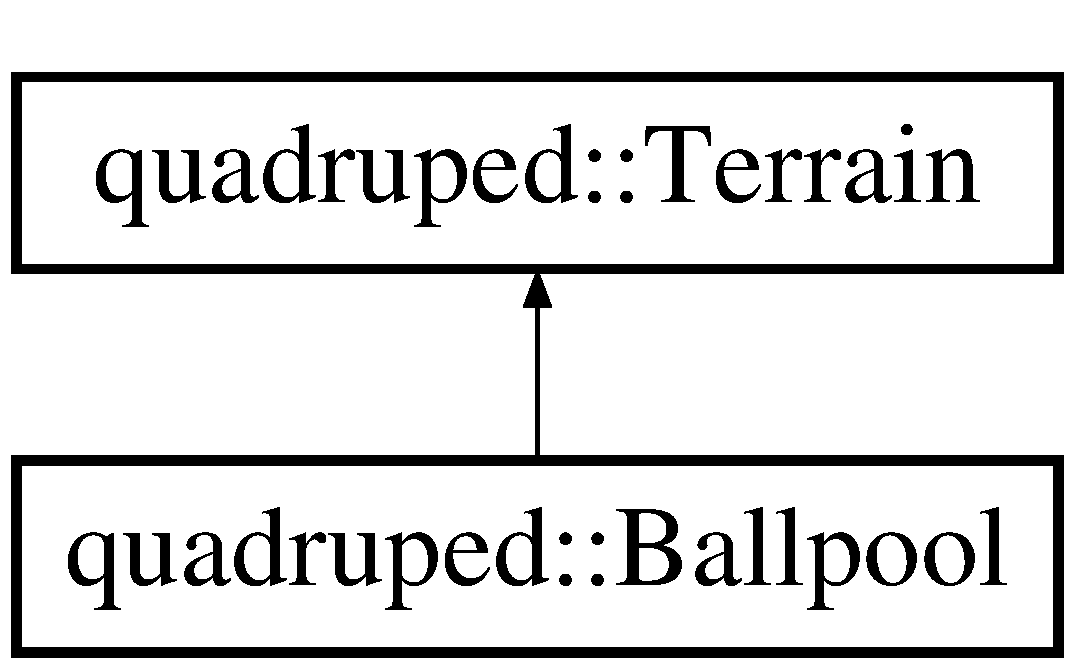
\includegraphics[height=2.000000cm]{classquadruped_1_1Ballpool}
\end{center}
\end{figure}
\subsection*{Public 成员函数}
\begin{DoxyCompactItemize}
\item 
\mbox{\Hypertarget{classquadruped_1_1Ballpool_a7ed536c8c14cf9e7bb19f243889e8c47}\label{classquadruped_1_1Ballpool_a7ed536c8c14cf9e7bb19f243889e8c47}} 
virtual double {\bfseries Get\+Hight} (double p\+\_\+x, double p\+\_\+y) override
\item 
\mbox{\Hypertarget{classquadruped_1_1Ballpool_a8fa06fc071ec30411adf16335319f405}\label{classquadruped_1_1Ballpool_a8fa06fc071ec30411adf16335319f405}} 
virtual void {\bfseries Updata\+Edge} (double p\+\_\+first\+\_\+edge\+\_\+\+D\+\_\+x, double p\+\_\+first\+\_\+edge\+\_\+\+D\+\_\+y) override
\item 
\mbox{\Hypertarget{classquadruped_1_1Ballpool_ac7775cd2a06a8f068890cb13841e40e5}\label{classquadruped_1_1Ballpool_ac7775cd2a06a8f068890cb13841e40e5}} 
virtual \hyperlink{cppTypes_8h_a65c27bf97693676535dd0b30ea0ad399}{Vec3}$<$ double $>$ {\bfseries Get\+Normal\+Vector} (double p\+\_\+x, double p\+\_\+y) override
\end{DoxyCompactItemize}
\subsection*{额外继承的成员函数}


该类的文档由以下文件生成\+:\begin{DoxyCompactItemize}
\item 
controller/motion\+Plan/terrain/\hyperlink{terrain_8hpp}{terrain.\+hpp}\item 
controller/motion\+Plan/terrain/\hyperlink{terrain_8cpp}{terrain.\+cpp}\end{DoxyCompactItemize}

\hypertarget{structbeeline__t}{}\section{beeline\+\_\+t结构体 参考}
\label{structbeeline__t}\index{beeline\+\_\+t@{beeline\+\_\+t}}


摆动腿足端轨迹规划相关结构体  




{\ttfamily \#include $<$cpp\+Struct.\+h$>$}

\subsection*{Public 属性}
\begin{DoxyCompactItemize}
\item 
\mbox{\Hypertarget{structbeeline__t_a6568a89c44f807b1d3a6e87dded6ca9a}\label{structbeeline__t_a6568a89c44f807b1d3a6e87dded6ca9a}} 
double {\bfseries lineA}
\item 
\mbox{\Hypertarget{structbeeline__t_a252082cc48884b3dc790cb0be82922db}\label{structbeeline__t_a252082cc48884b3dc790cb0be82922db}} 
double {\bfseries lineB}
\item 
\mbox{\Hypertarget{structbeeline__t_a45cd6263427cd0ae80f1de4f7bf82fbb}\label{structbeeline__t_a45cd6263427cd0ae80f1de4f7bf82fbb}} 
double {\bfseries lineC}
\end{DoxyCompactItemize}


\subsection{详细描述}
摆动腿足端轨迹规划相关结构体 

该结构体的文档由以下文件生成\+:\begin{DoxyCompactItemize}
\item 
\hyperlink{cppStruct_8h}{cpp\+Struct.\+h}\end{DoxyCompactItemize}

\hypertarget{classquadruped_1_1BodyOriTask}{}\section{quadruped\+:\+:Body\+Ori\+Task类 参考}
\label{classquadruped_1_1BodyOriTask}\index{quadruped\+::\+Body\+Ori\+Task@{quadruped\+::\+Body\+Ori\+Task}}
类 quadruped\+:\+:Body\+Ori\+Task 继承关系图\+:\begin{figure}[H]
\begin{center}
\leavevmode
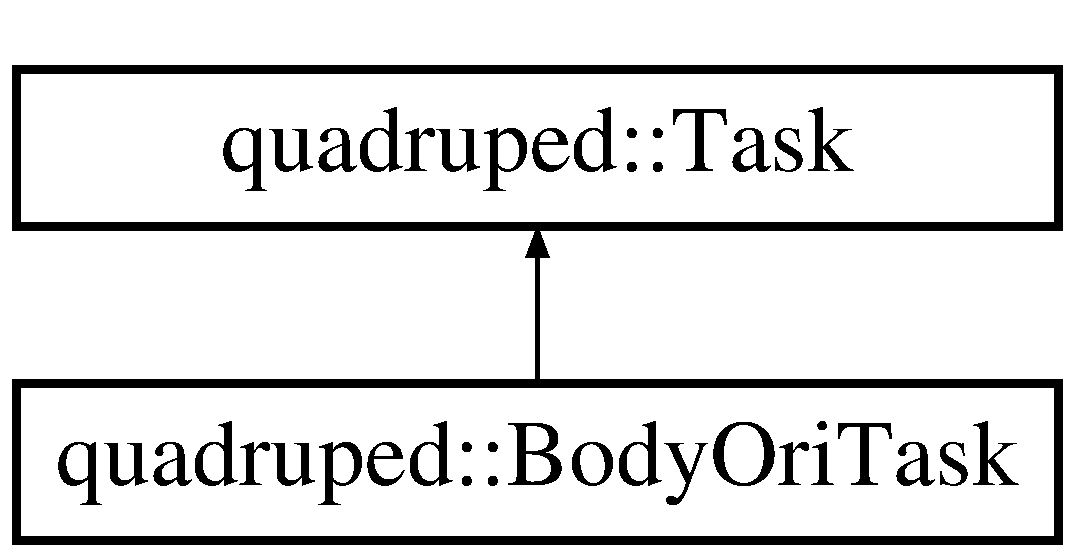
\includegraphics[height=2.000000cm]{classquadruped_1_1BodyOriTask}
\end{center}
\end{figure}
\subsection*{Public 成员函数}
\begin{DoxyCompactItemize}
\item 
\mbox{\Hypertarget{classquadruped_1_1BodyOriTask_aaaacfbc2ce8eb6024c82c0e7beb00376}\label{classquadruped_1_1BodyOriTask_aaaacfbc2ce8eb6024c82c0e7beb00376}} 
{\bfseries Body\+Ori\+Task} (\hyperlink{classquadruped_1_1RobotModel}{Robot\+Model} $\ast$p\+\_\+robot\+Model)
\end{DoxyCompactItemize}
\subsection*{Public 属性}
\begin{DoxyCompactItemize}
\item 
\mbox{\Hypertarget{classquadruped_1_1BodyOriTask_a3cfa0ce1162d634cbeb58a4780abd2f8}\label{classquadruped_1_1BodyOriTask_a3cfa0ce1162d634cbeb58a4780abd2f8}} 
\hyperlink{cppTypes_8h_a65c27bf97693676535dd0b30ea0ad399}{Vec3}$<$ double $>$ {\bfseries kp\+\_\+kin}
\item 
\mbox{\Hypertarget{classquadruped_1_1BodyOriTask_ab64b846d7752a46eb7e695aeb55ddd16}\label{classquadruped_1_1BodyOriTask_ab64b846d7752a46eb7e695aeb55ddd16}} 
\hyperlink{cppTypes_8h_a65c27bf97693676535dd0b30ea0ad399}{Vec3}$<$ double $>$ {\bfseries kp}
\item 
\mbox{\Hypertarget{classquadruped_1_1BodyOriTask_a04f5e3aaed16856a53564975b3d4e56a}\label{classquadruped_1_1BodyOriTask_a04f5e3aaed16856a53564975b3d4e56a}} 
\hyperlink{cppTypes_8h_a65c27bf97693676535dd0b30ea0ad399}{Vec3}$<$ double $>$ {\bfseries kd}
\end{DoxyCompactItemize}
\subsection*{Protected 成员函数}
\begin{DoxyCompactItemize}
\item 
\mbox{\Hypertarget{classquadruped_1_1BodyOriTask_a7f75d27666eaae52bb5b2a9a1ac7b8f3}\label{classquadruped_1_1BodyOriTask_a7f75d27666eaae52bb5b2a9a1ac7b8f3}} 
virtual bool {\bfseries Update\+Command} (const \hyperlink{cppTypes_8h_adad69baca3c77d5f991be5d3c063fea7}{D\+Vec}$<$ double $>$ \&p\+\_\+pos\+\_\+des, const \hyperlink{cppTypes_8h_adad69baca3c77d5f991be5d3c063fea7}{D\+Vec}$<$ double $>$ \&p\+\_\+vel\+\_\+des, const \hyperlink{cppTypes_8h_adad69baca3c77d5f991be5d3c063fea7}{D\+Vec}$<$ double $>$ \&p\+\_\+acc\+\_\+des)
\item 
\mbox{\Hypertarget{classquadruped_1_1BodyOriTask_a8e586844e192c0dadafc4f9f2157bb86}\label{classquadruped_1_1BodyOriTask_a8e586844e192c0dadafc4f9f2157bb86}} 
virtual bool {\bfseries Update\+Task\+Jacobian} (void)
\item 
\mbox{\Hypertarget{classquadruped_1_1BodyOriTask_a9697740e61b011bfe7847840e1dce00e}\label{classquadruped_1_1BodyOriTask_a9697740e61b011bfe7847840e1dce00e}} 
virtual bool {\bfseries Update\+Task\+J\+Dot\+Qdot} (void)
\item 
\mbox{\Hypertarget{classquadruped_1_1BodyOriTask_a810528aef22f9c6ba0949e35e1fcf397}\label{classquadruped_1_1BodyOriTask_a810528aef22f9c6ba0949e35e1fcf397}} 
virtual bool {\bfseries Additional\+Update} (void)
\end{DoxyCompactItemize}
\subsection*{Protected 属性}
\begin{DoxyCompactItemize}
\item 
\mbox{\Hypertarget{classquadruped_1_1BodyOriTask_ac7a9a5bd9b8239af3cb68e49d0a1b0a0}\label{classquadruped_1_1BodyOriTask_ac7a9a5bd9b8239af3cb68e49d0a1b0a0}} 
\hyperlink{classquadruped_1_1RobotModel}{Robot\+Model} $\ast$ {\bfseries robot\+Model}
\end{DoxyCompactItemize}


该类的文档由以下文件生成\+:\begin{DoxyCompactItemize}
\item 
controller/wbc/task\+Set/body\+Ori\+Task.\+hpp\item 
controller/wbc/task\+Set/\hyperlink{bodyOriTask_8cpp}{body\+Ori\+Task.\+cpp}\end{DoxyCompactItemize}

\hypertarget{classquadruped_1_1BodyPosTask}{}\section{quadruped\+:\+:Body\+Pos\+Task类 参考}
\label{classquadruped_1_1BodyPosTask}\index{quadruped\+::\+Body\+Pos\+Task@{quadruped\+::\+Body\+Pos\+Task}}
类 quadruped\+:\+:Body\+Pos\+Task 继承关系图\+:\begin{figure}[H]
\begin{center}
\leavevmode
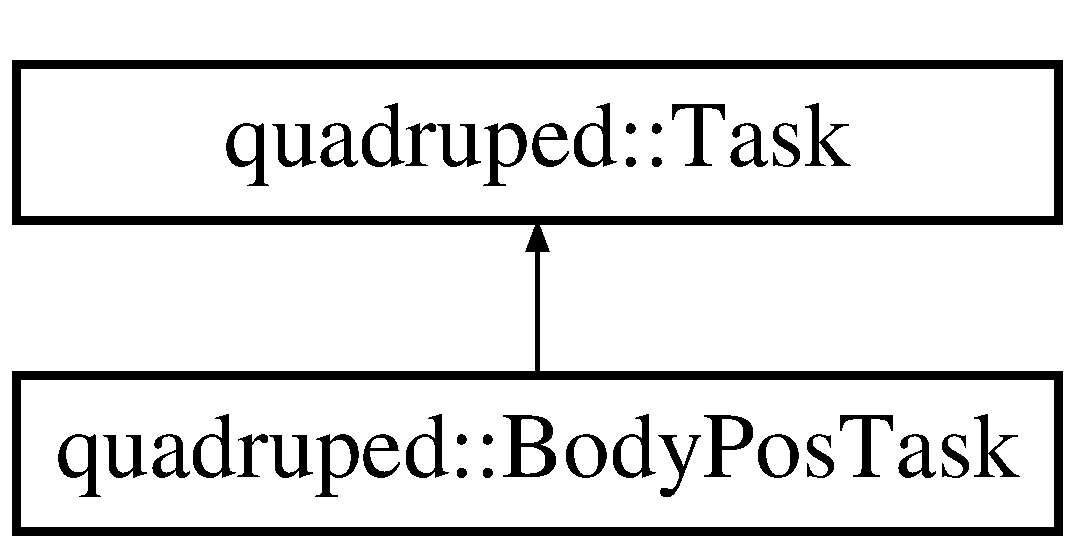
\includegraphics[height=2.000000cm]{classquadruped_1_1BodyPosTask}
\end{center}
\end{figure}
\subsection*{Public 成员函数}
\begin{DoxyCompactItemize}
\item 
\mbox{\Hypertarget{classquadruped_1_1BodyPosTask_acf0fdb410e5f268e42e0fb73a30e5a10}\label{classquadruped_1_1BodyPosTask_acf0fdb410e5f268e42e0fb73a30e5a10}} 
{\bfseries Body\+Pos\+Task} (\hyperlink{classquadruped_1_1RobotModel}{Robot\+Model} $\ast$p\+\_\+robot\+Model)
\end{DoxyCompactItemize}
\subsection*{Public 属性}
\begin{DoxyCompactItemize}
\item 
\mbox{\Hypertarget{classquadruped_1_1BodyPosTask_a4379b09405855a253d4d3696d06d6f14}\label{classquadruped_1_1BodyPosTask_a4379b09405855a253d4d3696d06d6f14}} 
\hyperlink{cppTypes_8h_a65c27bf97693676535dd0b30ea0ad399}{Vec3}$<$ double $>$ {\bfseries kp\+\_\+kin}
\item 
\mbox{\Hypertarget{classquadruped_1_1BodyPosTask_a4a898057ecf94be2a49f7ee05ef4a378}\label{classquadruped_1_1BodyPosTask_a4a898057ecf94be2a49f7ee05ef4a378}} 
\hyperlink{cppTypes_8h_a65c27bf97693676535dd0b30ea0ad399}{Vec3}$<$ double $>$ {\bfseries kp}
\item 
\mbox{\Hypertarget{classquadruped_1_1BodyPosTask_aa5d74c4423fe591e58aa11a6b32b7d96}\label{classquadruped_1_1BodyPosTask_aa5d74c4423fe591e58aa11a6b32b7d96}} 
\hyperlink{cppTypes_8h_a65c27bf97693676535dd0b30ea0ad399}{Vec3}$<$ double $>$ {\bfseries kd}
\end{DoxyCompactItemize}
\subsection*{Protected 成员函数}
\begin{DoxyCompactItemize}
\item 
\mbox{\Hypertarget{classquadruped_1_1BodyPosTask_a252a17077072aa17e605039aaaa904d5}\label{classquadruped_1_1BodyPosTask_a252a17077072aa17e605039aaaa904d5}} 
virtual bool {\bfseries Update\+Command} (const \hyperlink{cppTypes_8h_adad69baca3c77d5f991be5d3c063fea7}{D\+Vec}$<$ double $>$ \&p\+\_\+pos\+\_\+des, const \hyperlink{cppTypes_8h_adad69baca3c77d5f991be5d3c063fea7}{D\+Vec}$<$ double $>$ \&p\+\_\+vel\+\_\+des, const \hyperlink{cppTypes_8h_adad69baca3c77d5f991be5d3c063fea7}{D\+Vec}$<$ double $>$ \&p\+\_\+acc\+\_\+des)
\item 
\mbox{\Hypertarget{classquadruped_1_1BodyPosTask_a6b186be3525538677f261a91d574fea2}\label{classquadruped_1_1BodyPosTask_a6b186be3525538677f261a91d574fea2}} 
virtual bool {\bfseries Update\+Task\+Jacobian} (void)
\item 
\mbox{\Hypertarget{classquadruped_1_1BodyPosTask_a73b5e34cea057b2f9e84b207a40d9a37}\label{classquadruped_1_1BodyPosTask_a73b5e34cea057b2f9e84b207a40d9a37}} 
virtual bool {\bfseries Update\+Task\+J\+Dot\+Qdot} (void)
\item 
\mbox{\Hypertarget{classquadruped_1_1BodyPosTask_a1654f33f0e1435b97811a037b2d6f9ea}\label{classquadruped_1_1BodyPosTask_a1654f33f0e1435b97811a037b2d6f9ea}} 
virtual bool {\bfseries Additional\+Update} (void)
\end{DoxyCompactItemize}
\subsection*{Protected 属性}
\begin{DoxyCompactItemize}
\item 
\mbox{\Hypertarget{classquadruped_1_1BodyPosTask_ab6b7abbe217b1d765e0fd1e0a44d0d8e}\label{classquadruped_1_1BodyPosTask_ab6b7abbe217b1d765e0fd1e0a44d0d8e}} 
\hyperlink{classquadruped_1_1RobotModel}{Robot\+Model} $\ast$ {\bfseries robot\+Model}
\end{DoxyCompactItemize}


该类的文档由以下文件生成\+:\begin{DoxyCompactItemize}
\item 
controller/wbc/task\+Set/body\+Pos\+Task.\+hpp\item 
controller/wbc/task\+Set/\hyperlink{bodyPosTask_8cpp}{body\+Pos\+Task.\+cpp}\end{DoxyCompactItemize}

\hypertarget{classquadruped_1_1BodyStateEstimate}{}\section{quadruped\+:\+:Body\+State\+Estimate类 参考}
\label{classquadruped_1_1BodyStateEstimate}\index{quadruped\+::\+Body\+State\+Estimate@{quadruped\+::\+Body\+State\+Estimate}}


Actiger机体状态信息类  




{\ttfamily \#include $<$body\+State\+Estimate.\+hpp$>$}

\subsection*{Public 成员函数}
\begin{DoxyCompactItemize}
\item 
\mbox{\Hypertarget{classquadruped_1_1BodyStateEstimate_a3b0db8c7b7cf21b040f3fbe15dd02b7e}\label{classquadruped_1_1BodyStateEstimate_a3b0db8c7b7cf21b040f3fbe15dd02b7e}} 
\hyperlink{classquadruped_1_1BodyStateEstimate_a3b0db8c7b7cf21b040f3fbe15dd02b7e}{Body\+State\+Estimate} (void)
\begin{DoxyCompactList}\small\item\em Body\+State\+Estimate类的构造函数，完成所有对象成员的内存分配以及数据成员的初值装载 \end{DoxyCompactList}\item 
\mbox{\Hypertarget{classquadruped_1_1BodyStateEstimate_ae223eff98ecc03c171df9c97db54a0d0}\label{classquadruped_1_1BodyStateEstimate_ae223eff98ecc03c171df9c97db54a0d0}} 
virtual \hyperlink{classquadruped_1_1BodyStateEstimate_ae223eff98ecc03c171df9c97db54a0d0}{$\sim$\+Body\+State\+Estimate} (void)
\begin{DoxyCompactList}\small\item\em Body\+State\+Estimate类的析构函数，释放申请的内存 \end{DoxyCompactList}\item 
\mbox{\Hypertarget{classquadruped_1_1BodyStateEstimate_ab731b3e8b88e419328d057a90df7819d}\label{classquadruped_1_1BodyStateEstimate_ab731b3e8b88e419328d057a90df7819d}} 
void {\bfseries Get\+Robot\+Msg} (\hyperlink{classquadruped_1_1LegStateEstimate}{Leg\+State\+Estimate} $\ast$p\+\_\+lf\+\_\+leg\+State, \hyperlink{classquadruped_1_1LegStateEstimate}{Leg\+State\+Estimate} $\ast$p\+\_\+lr\+\_\+leg\+State, \hyperlink{classquadruped_1_1LegStateEstimate}{Leg\+State\+Estimate} $\ast$p\+\_\+rf\+\_\+leg\+State, \hyperlink{classquadruped_1_1LegStateEstimate}{Leg\+State\+Estimate} $\ast$p\+\_\+rr\+\_\+leg\+State, \hyperlink{cppTypes_8h_a87f228860242acc66da2e58086d18cec}{Vec12}$<$ double $>$ p\+\_\+f\+\_\+k, \hyperlink{cppTypes_8h_a87f228860242acc66da2e58086d18cec}{Vec12}$<$ double $>$ p\+\_\+f\+\_\+k\+\_\+1, \hyperlink{cppTypes_8h_a65c27bf97693676535dd0b30ea0ad399}{Vec3}$<$ double $>$ p\+\_\+actul\+\_\+body\+\_\+acc)
\end{DoxyCompactItemize}
\subsection*{Public 属性}
\begin{DoxyCompactItemize}
\item 
\mbox{\Hypertarget{classquadruped_1_1BodyStateEstimate_aa35c4d3cccbe97d87b67f905a053e511}\label{classquadruped_1_1BodyStateEstimate_aa35c4d3cccbe97d87b67f905a053e511}} 
\hyperlink{cppTypes_8h_a65c27bf97693676535dd0b30ea0ad399}{Vec3}$<$ double $>$ \hyperlink{classquadruped_1_1BodyStateEstimate_aa35c4d3cccbe97d87b67f905a053e511}{actul\+\_\+body\+\_\+pos}
\begin{DoxyCompactList}\small\item\em Actiger在全局坐标系下的实际位置 \end{DoxyCompactList}\item 
\mbox{\Hypertarget{classquadruped_1_1BodyStateEstimate_ac1876f2fe4e195c02503fc226df19739}\label{classquadruped_1_1BodyStateEstimate_ac1876f2fe4e195c02503fc226df19739}} 
\hyperlink{cppTypes_8h_a65c27bf97693676535dd0b30ea0ad399}{Vec3}$<$ double $>$ \hyperlink{classquadruped_1_1BodyStateEstimate_ac1876f2fe4e195c02503fc226df19739}{actul\+\_\+body\+\_\+vel}
\begin{DoxyCompactList}\small\item\em Actiger在惯性坐标系下的实际速度 \end{DoxyCompactList}\item 
\mbox{\Hypertarget{classquadruped_1_1BodyStateEstimate_a89d1158f1e3d79c258a16c04b6e8462e}\label{classquadruped_1_1BodyStateEstimate_a89d1158f1e3d79c258a16c04b6e8462e}} 
\hyperlink{cppTypes_8h_a65c27bf97693676535dd0b30ea0ad399}{Vec3}$<$ double $>$ \hyperlink{classquadruped_1_1BodyStateEstimate_a89d1158f1e3d79c258a16c04b6e8462e}{actul\+\_\+body\+\_\+angle}
\begin{DoxyCompactList}\small\item\em Actiger在惯性坐标系下的实际欧拉角 \end{DoxyCompactList}\item 
\mbox{\Hypertarget{classquadruped_1_1BodyStateEstimate_a7529e7a4536cbed8f25b28ca61f038dc}\label{classquadruped_1_1BodyStateEstimate_a7529e7a4536cbed8f25b28ca61f038dc}} 
\hyperlink{cppTypes_8h_a65c27bf97693676535dd0b30ea0ad399}{Vec3}$<$ double $>$ \hyperlink{classquadruped_1_1BodyStateEstimate_a7529e7a4536cbed8f25b28ca61f038dc}{actul\+\_\+body\+\_\+angular\+Vel}
\begin{DoxyCompactList}\small\item\em Actiger在惯性坐标系下的实际欧拉角速度 \end{DoxyCompactList}\item 
\mbox{\Hypertarget{classquadruped_1_1BodyStateEstimate_aefe6bd47e63f09418b59581b057fb59c}\label{classquadruped_1_1BodyStateEstimate_aefe6bd47e63f09418b59581b057fb59c}} 
\hyperlink{cppTypes_8h_adb7d462b35d31f0b2583b3e230a2a2c3}{Mat3}$<$ double $>$ \hyperlink{classquadruped_1_1BodyStateEstimate_aefe6bd47e63f09418b59581b057fb59c}{rotation}
\begin{DoxyCompactList}\small\item\em Actiger从机体到世界的旋转矩阵 \end{DoxyCompactList}\item 
\mbox{\Hypertarget{classquadruped_1_1BodyStateEstimate_a2970e450281c6c3c292f374d0ba270dd}\label{classquadruped_1_1BodyStateEstimate_a2970e450281c6c3c292f374d0ba270dd}} 
double {\bfseries z\+\_\+offset}
\item 
\mbox{\Hypertarget{classquadruped_1_1BodyStateEstimate_a33cb43c18bb3321dc8dd4ce73c806ad6}\label{classquadruped_1_1BodyStateEstimate_a33cb43c18bb3321dc8dd4ce73c806ad6}} 
double {\bfseries position\+\_\+x\+\_\+}
\item 
\mbox{\Hypertarget{classquadruped_1_1BodyStateEstimate_ab9f2b9c71c9f7b534b88a5c32a822048}\label{classquadruped_1_1BodyStateEstimate_ab9f2b9c71c9f7b534b88a5c32a822048}} 
double {\bfseries position\+\_\+y\+\_\+}
\item 
\mbox{\Hypertarget{classquadruped_1_1BodyStateEstimate_a4dc9b7e4c4728fafb92b9b3542617b99}\label{classquadruped_1_1BodyStateEstimate_a4dc9b7e4c4728fafb92b9b3542617b99}} 
double {\bfseries position\+\_\+z\+\_\+}
\item 
\mbox{\Hypertarget{classquadruped_1_1BodyStateEstimate_a6ec290fad3636ce035b5f77cc8776cc6}\label{classquadruped_1_1BodyStateEstimate_a6ec290fad3636ce035b5f77cc8776cc6}} 
\hyperlink{cppTypes_8h_a65c27bf97693676535dd0b30ea0ad399}{Vec3}$<$ double $>$ {\bfseries body\+Pos\+World}
\item 
\mbox{\Hypertarget{classquadruped_1_1BodyStateEstimate_a5e504f77a67dad88923a1c366227437b}\label{classquadruped_1_1BodyStateEstimate_a5e504f77a67dad88923a1c366227437b}} 
int {\bfseries cnt}
\item 
\mbox{\Hypertarget{classquadruped_1_1BodyStateEstimate_a81bd0b9aa8dce20696856eefb5431b1c}\label{classquadruped_1_1BodyStateEstimate_a81bd0b9aa8dce20696856eefb5431b1c}} 
\hyperlink{classVelocityEstimate}{Velocity\+Estimate} $\ast$ {\bfseries velocity\+Estimate}
\end{DoxyCompactItemize}


\subsection{详细描述}
Actiger机体状态信息类 

该类的文档由以下文件生成\+:\begin{DoxyCompactItemize}
\item 
controller/model/\hyperlink{bodyStateEstimate_8hpp}{body\+State\+Estimate.\+hpp}\item 
controller/model/\hyperlink{bodyStateEstimate_8cpp}{body\+State\+Estimate.\+cpp}\end{DoxyCompactItemize}

\hypertarget{classquadruped_1_1BodyTrajectory}{}\section{quadruped\+:\+:Body\+Trajectory类 参考}
\label{classquadruped_1_1BodyTrajectory}\index{quadruped\+::\+Body\+Trajectory@{quadruped\+::\+Body\+Trajectory}}
\subsection*{Public 成员函数}
\begin{DoxyCompactItemize}
\item 
\mbox{\Hypertarget{classquadruped_1_1BodyTrajectory_a676f710f4d779a54461a74fc2466b831}\label{classquadruped_1_1BodyTrajectory_a676f710f4d779a54461a74fc2466b831}} 
{\bfseries Body\+Trajectory} (\hyperlink{classquadruped_1_1Parameters}{Parameters} $\ast$p\+\_\+para)
\item 
void \hyperlink{classquadruped_1_1BodyTrajectory_ae7dfc17baf5ea44b346b3ee7bc7c2cea}{Get\+Body\+Trajectory} (void)
\item 
void \hyperlink{classquadruped_1_1BodyTrajectory_a633b42ab0022c3cedeb719287e9ae9b2}{Update\+Info} (bool p\+\_\+is\+\_\+lf\+\_\+rr\+\_\+stand, double p\+\_\+\+Ts, \hyperlink{cppTypes_8h_a27bb8a600520708a5928332e4e52a92e}{Vec6}$<$ double $>$ p\+\_\+spatial\+\_\+now, \hyperlink{cppTypes_8h_a27bb8a600520708a5928332e4e52a92e}{Vec6}$<$ double $>$ p\+\_\+spatial\+\_\+dot\+\_\+now, \hyperlink{cppTypes_8h_a27bb8a600520708a5928332e4e52a92e}{Vec6}$<$ double $>$ p\+\_\+spatial\+\_\+des, \hyperlink{cppTypes_8h_a27bb8a600520708a5928332e4e52a92e}{Vec6}$<$ double $>$ p\+\_\+spatial\+\_\+dot\+\_\+des)
\end{DoxyCompactItemize}
\subsection*{Public 属性}
\begin{DoxyCompactItemize}
\item 
\mbox{\Hypertarget{classquadruped_1_1BodyTrajectory_a7b8fc2a7a4460107e6270cc48f1ee32b}\label{classquadruped_1_1BodyTrajectory_a7b8fc2a7a4460107e6270cc48f1ee32b}} 
double {\bfseries Ts}
\item 
\mbox{\Hypertarget{classquadruped_1_1BodyTrajectory_a604fd9c50ea5bd2e97e0625a601f6a0c}\label{classquadruped_1_1BodyTrajectory_a604fd9c50ea5bd2e97e0625a601f6a0c}} 
int {\bfseries grid}
\item 
\mbox{\Hypertarget{classquadruped_1_1BodyTrajectory_aa01d92e051dd84c8b321f52280d1f614}\label{classquadruped_1_1BodyTrajectory_aa01d92e051dd84c8b321f52280d1f614}} 
\hyperlink{cppTypes_8h_a65c27bf97693676535dd0b30ea0ad399}{Vec3}$<$ double $>$ {\bfseries normal\+\_\+vec}
\item 
\mbox{\Hypertarget{classquadruped_1_1BodyTrajectory_a6b47f6fd369a25e35cc1c354d8fb1c26}\label{classquadruped_1_1BodyTrajectory_a6b47f6fd369a25e35cc1c354d8fb1c26}} 
bool {\bfseries is\+\_\+lf\+\_\+rr\+\_\+stand}
\item 
\mbox{\Hypertarget{classquadruped_1_1BodyTrajectory_a29765f40198f6c5ff7ba1f559a74d949}\label{classquadruped_1_1BodyTrajectory_a29765f40198f6c5ff7ba1f559a74d949}} 
\hyperlink{cppTypes_8h_a65c27bf97693676535dd0b30ea0ad399}{Vec3}$<$ double $>$ {\bfseries lf\+\_\+hip\+\_\+pos\+\_\+body}
\item 
\mbox{\Hypertarget{classquadruped_1_1BodyTrajectory_a8d774f9e415f59453cef14fdaea86a09}\label{classquadruped_1_1BodyTrajectory_a8d774f9e415f59453cef14fdaea86a09}} 
\hyperlink{cppTypes_8h_a65c27bf97693676535dd0b30ea0ad399}{Vec3}$<$ double $>$ {\bfseries lr\+\_\+hip\+\_\+pos\+\_\+body}
\item 
\mbox{\Hypertarget{classquadruped_1_1BodyTrajectory_a0107c8a6d523735966be78745a7ea5d3}\label{classquadruped_1_1BodyTrajectory_a0107c8a6d523735966be78745a7ea5d3}} 
\hyperlink{cppTypes_8h_a65c27bf97693676535dd0b30ea0ad399}{Vec3}$<$ double $>$ {\bfseries rf\+\_\+hip\+\_\+pos\+\_\+body}
\item 
\mbox{\Hypertarget{classquadruped_1_1BodyTrajectory_a9f81343660bef07259e20b6b14ce9765}\label{classquadruped_1_1BodyTrajectory_a9f81343660bef07259e20b6b14ce9765}} 
\hyperlink{cppTypes_8h_a65c27bf97693676535dd0b30ea0ad399}{Vec3}$<$ double $>$ {\bfseries rr\+\_\+hip\+\_\+pos\+\_\+body}
\item 
\mbox{\Hypertarget{classquadruped_1_1BodyTrajectory_aa76ebbb50d72eccc103e440964fd13c9}\label{classquadruped_1_1BodyTrajectory_aa76ebbb50d72eccc103e440964fd13c9}} 
\hyperlink{cppTypes_8h_a5db6bfb25afa103db1fb6bb6287ae9d7}{D\+Mat}$<$ double $>$ {\bfseries return\+\_\+spatial\+\_\+list}
\item 
\mbox{\Hypertarget{classquadruped_1_1BodyTrajectory_a1e8e9999a703a26ccff586073d3347ee}\label{classquadruped_1_1BodyTrajectory_a1e8e9999a703a26ccff586073d3347ee}} 
\hyperlink{cppTypes_8h_a5db6bfb25afa103db1fb6bb6287ae9d7}{D\+Mat}$<$ double $>$ {\bfseries return\+\_\+spatial\+\_\+dot\+\_\+list}
\end{DoxyCompactItemize}


\subsection{成员函数说明}
\mbox{\Hypertarget{classquadruped_1_1BodyTrajectory_ae7dfc17baf5ea44b346b3ee7bc7c2cea}\label{classquadruped_1_1BodyTrajectory_ae7dfc17baf5ea44b346b3ee7bc7c2cea}} 
\index{quadruped\+::\+Body\+Trajectory@{quadruped\+::\+Body\+Trajectory}!Get\+Body\+Trajectory@{Get\+Body\+Trajectory}}
\index{Get\+Body\+Trajectory@{Get\+Body\+Trajectory}!quadruped\+::\+Body\+Trajectory@{quadruped\+::\+Body\+Trajectory}}
\subsubsection{\texorpdfstring{Get\+Body\+Trajectory()}{GetBodyTrajectory()}}
{\footnotesize\ttfamily void Body\+Trajectory\+::\+Get\+Body\+Trajectory (\begin{DoxyParamCaption}\item[{void}]{ }\end{DoxyParamCaption})}

\+: 获取机体轨迹 
\begin{DoxyParams}{参数}
{\em \{$\ast$\}} & \\
\hline
\end{DoxyParams}
\begin{DoxyReturn}{返回}
\{$\ast$\} 
\end{DoxyReturn}


参考 quadruped\+::dim\+\_\+floating , 以及 M\+P\+C\+\_\+\+P\+E\+R\+I\+OD.

\mbox{\Hypertarget{classquadruped_1_1BodyTrajectory_a633b42ab0022c3cedeb719287e9ae9b2}\label{classquadruped_1_1BodyTrajectory_a633b42ab0022c3cedeb719287e9ae9b2}} 
\index{quadruped\+::\+Body\+Trajectory@{quadruped\+::\+Body\+Trajectory}!Update\+Info@{Update\+Info}}
\index{Update\+Info@{Update\+Info}!quadruped\+::\+Body\+Trajectory@{quadruped\+::\+Body\+Trajectory}}
\subsubsection{\texorpdfstring{Update\+Info()}{UpdateInfo()}}
{\footnotesize\ttfamily void Body\+Trajectory\+::\+Update\+Info (\begin{DoxyParamCaption}\item[{bool}]{p\+\_\+is\+\_\+lf\+\_\+rr\+\_\+stand,  }\item[{double}]{p\+\_\+\+Ts,  }\item[{\hyperlink{cppTypes_8h_a27bb8a600520708a5928332e4e52a92e}{Vec6}$<$ double $>$}]{p\+\_\+spatial\+\_\+now,  }\item[{\hyperlink{cppTypes_8h_a27bb8a600520708a5928332e4e52a92e}{Vec6}$<$ double $>$}]{p\+\_\+spatial\+\_\+dot\+\_\+now,  }\item[{\hyperlink{cppTypes_8h_a27bb8a600520708a5928332e4e52a92e}{Vec6}$<$ double $>$}]{p\+\_\+spatial\+\_\+des,  }\item[{\hyperlink{cppTypes_8h_a27bb8a600520708a5928332e4e52a92e}{Vec6}$<$ double $>$}]{p\+\_\+spatial\+\_\+dot\+\_\+des }\end{DoxyParamCaption})}

\+: 更新机体轨迹规划器的信息 
\begin{DoxyParams}{参数}
{\em \{$\ast$\}} & \\
\hline
\end{DoxyParams}
\begin{DoxyReturn}{返回}
\{$\ast$\} 
\end{DoxyReturn}


参考 M\+P\+C\+\_\+\+P\+E\+R\+I\+OD.



该类的文档由以下文件生成\+:\begin{DoxyCompactItemize}
\item 
controller/motion\+Plan/body\+Trajectory/body\+Trajectory.\+hpp\item 
controller/motion\+Plan/body\+Trajectory/body\+Trajectory.\+cpp\end{DoxyCompactItemize}

\hypertarget{classquadruped_1_1Bridge}{}\section{quadruped\+:\+:Bridge类 参考}
\label{classquadruped_1_1Bridge}\index{quadruped\+::\+Bridge@{quadruped\+::\+Bridge}}


双木桥类子类  




{\ttfamily \#include $<$terrain.\+hpp$>$}

类 quadruped\+:\+:Bridge 继承关系图\+:\begin{figure}[H]
\begin{center}
\leavevmode
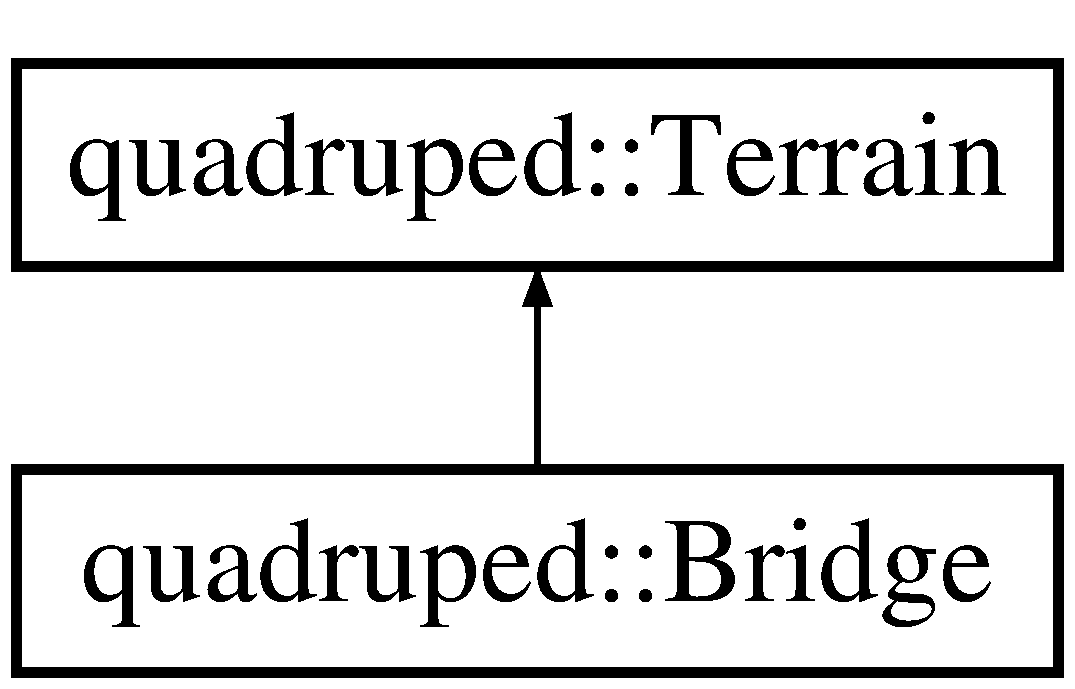
\includegraphics[height=2.000000cm]{classquadruped_1_1Bridge}
\end{center}
\end{figure}
\subsection*{Public 成员函数}
\begin{DoxyCompactItemize}
\item 
\mbox{\Hypertarget{classquadruped_1_1Bridge_a43a5f86e9314079462fad0d08c27b880}\label{classquadruped_1_1Bridge_a43a5f86e9314079462fad0d08c27b880}} 
\hyperlink{classquadruped_1_1Bridge_a43a5f86e9314079462fad0d08c27b880}{Bridge} (void)
\begin{DoxyCompactList}\small\item\em Bridge类的构造函数，完成地形标识符以及地形分割线的初始化 \end{DoxyCompactList}\item 
virtual double \hyperlink{classquadruped_1_1Bridge_a6253ac813ba0f6032e31f1ed183014be}{Get\+Hight} (double p\+\_\+x, double p\+\_\+y) override
\begin{DoxyCompactList}\small\item\em 获取当前地形在世界坐标系下的高度 \end{DoxyCompactList}\item 
virtual void \hyperlink{classquadruped_1_1Bridge_a6919abf7851a9dabacad2cf3af75ed5e}{Updata\+Edge} (double p\+\_\+first\+\_\+edge\+\_\+\+D\+\_\+x, double p\+\_\+first\+\_\+edge\+\_\+\+D\+\_\+y) override
\begin{DoxyCompactList}\small\item\em 获取双木桥与地面的交线中点在世界坐标系下的位置以及分割线和危险区的设置 \end{DoxyCompactList}\item 
virtual \hyperlink{cppTypes_8h_a65c27bf97693676535dd0b30ea0ad399}{Vec3}$<$ double $>$ \hyperlink{classquadruped_1_1Bridge_a545f85d2f11aa32b6341e32a39b6d1bf}{Get\+Normal\+Vector} (double p\+\_\+x, double p\+\_\+y) override
\begin{DoxyCompactList}\small\item\em 预留接口 $\vert$ 获取双木桥某一点处的法向量 \end{DoxyCompactList}\end{DoxyCompactItemize}
\subsection*{额外继承的成员函数}


\subsection{详细描述}
双木桥类子类 

\subsection{成员函数说明}
\mbox{\Hypertarget{classquadruped_1_1Bridge_a6253ac813ba0f6032e31f1ed183014be}\label{classquadruped_1_1Bridge_a6253ac813ba0f6032e31f1ed183014be}} 
\index{quadruped\+::\+Bridge@{quadruped\+::\+Bridge}!Get\+Hight@{Get\+Hight}}
\index{Get\+Hight@{Get\+Hight}!quadruped\+::\+Bridge@{quadruped\+::\+Bridge}}
\subsubsection{\texorpdfstring{Get\+Hight()}{GetHight()}}
{\footnotesize\ttfamily double Bridge\+::\+Get\+Hight (\begin{DoxyParamCaption}\item[{double}]{p\+\_\+x,  }\item[{double}]{p\+\_\+y }\end{DoxyParamCaption})\hspace{0.3cm}{\ttfamily [override]}, {\ttfamily [virtual]}}



获取当前地形在世界坐标系下的高度 


\begin{DoxyParams}{参数}
{\em p\+\_\+x} & 当前点在世界坐标系位置坐标的\+X值 \\
\hline
{\em p\+\_\+y} & 当前点在世界坐标系位置坐标的\+Y值 \\
\hline
\end{DoxyParams}
\begin{DoxyReturn}{返回}
double 
\end{DoxyReturn}


重载 \hyperlink{classquadruped_1_1Terrain}{quadruped\+::\+Terrain} .



参考 B\+R\+I\+D\+G\+E\+\_\+\+H\+E\+I\+G\+HT, B\+R\+I\+D\+G\+E\+\_\+\+L\+E\+N\+G\+TH , 以及 quadruped\+::\+Terrain\+::first\+\_\+edge\+\_\+\+D\+\_\+x.

\mbox{\Hypertarget{classquadruped_1_1Bridge_a545f85d2f11aa32b6341e32a39b6d1bf}\label{classquadruped_1_1Bridge_a545f85d2f11aa32b6341e32a39b6d1bf}} 
\index{quadruped\+::\+Bridge@{quadruped\+::\+Bridge}!Get\+Normal\+Vector@{Get\+Normal\+Vector}}
\index{Get\+Normal\+Vector@{Get\+Normal\+Vector}!quadruped\+::\+Bridge@{quadruped\+::\+Bridge}}
\subsubsection{\texorpdfstring{Get\+Normal\+Vector()}{GetNormalVector()}}
{\footnotesize\ttfamily \hyperlink{cppTypes_8h_a65c27bf97693676535dd0b30ea0ad399}{Vec3}$<$ double $>$ Bridge\+::\+Get\+Normal\+Vector (\begin{DoxyParamCaption}\item[{double}]{p\+\_\+x,  }\item[{double}]{p\+\_\+y }\end{DoxyParamCaption})\hspace{0.3cm}{\ttfamily [override]}, {\ttfamily [virtual]}}



预留接口 $\vert$ 获取双木桥某一点处的法向量 


\begin{DoxyParams}{参数}
{\em p\+\_\+x} & \\
\hline
{\em p\+\_\+y} & \\
\hline
\end{DoxyParams}
\begin{DoxyReturn}{返回}
Vec3$<$double$>$ 
\end{DoxyReturn}


实现了 \hyperlink{classquadruped_1_1Terrain}{quadruped\+::\+Terrain}.



参考 quadruped\+::\+Terrain\+::first\+\_\+edge\+\_\+\+D\+\_\+x.

\mbox{\Hypertarget{classquadruped_1_1Bridge_a6919abf7851a9dabacad2cf3af75ed5e}\label{classquadruped_1_1Bridge_a6919abf7851a9dabacad2cf3af75ed5e}} 
\index{quadruped\+::\+Bridge@{quadruped\+::\+Bridge}!Updata\+Edge@{Updata\+Edge}}
\index{Updata\+Edge@{Updata\+Edge}!quadruped\+::\+Bridge@{quadruped\+::\+Bridge}}
\subsubsection{\texorpdfstring{Updata\+Edge()}{UpdataEdge()}}
{\footnotesize\ttfamily void Bridge\+::\+Updata\+Edge (\begin{DoxyParamCaption}\item[{double}]{p\+\_\+first\+\_\+edge\+\_\+\+D\+\_\+x,  }\item[{double}]{p\+\_\+first\+\_\+edge\+\_\+\+D\+\_\+y }\end{DoxyParamCaption})\hspace{0.3cm}{\ttfamily [override]}, {\ttfamily [virtual]}}



获取双木桥与地面的交线中点在世界坐标系下的位置以及分割线和危险区的设置 


\begin{DoxyParams}{参数}
{\em p\+\_\+first\+\_\+edge\+\_\+\+D\+\_\+x} & 当前点在世界坐标系位置坐标的\+X值 \\
\hline
{\em p\+\_\+first\+\_\+edge\+\_\+\+D\+\_\+y} & 当前点在世界坐标系位置坐标的\+Y值 \\
\hline
\end{DoxyParams}


重载 \hyperlink{classquadruped_1_1Terrain}{quadruped\+::\+Terrain} .



参考 quadruped\+::\+Terrain\+::average\+Danger\+Area, B\+R\+I\+D\+G\+E\+\_\+\+H\+E\+I\+G\+HT, B\+R\+I\+D\+G\+E\+\_\+\+L\+E\+N\+G\+TH, quadruped\+::\+Terrain\+::first\+\_\+edge\+\_\+\+D\+\_\+x, quadruped\+::\+Terrain\+::first\+\_\+edge\+\_\+\+D\+\_\+y, L\+I\+M\+I\+T\+\_\+\+I\+N\+F\+I\+N\+I\+TE, quadruped\+::\+Terrain\+::num\+Split, quadruped\+::\+Terrain\+::safe\+Area , 以及 quadruped\+::\+Terrain\+::split.



该类的文档由以下文件生成\+:\begin{DoxyCompactItemize}
\item 
controller/motion\+Plan/terrain/\hyperlink{terrain_8hpp}{terrain.\+hpp}\item 
controller/motion\+Plan/terrain/\hyperlink{terrain_8cpp}{terrain.\+cpp}\end{DoxyCompactItemize}

\hypertarget{classquadruped_1_1Calandria}{}\section{quadruped\+:\+:Calandria类 参考}
\label{classquadruped_1_1Calandria}\index{quadruped\+::\+Calandria@{quadruped\+::\+Calandria}}


排管类子类  




{\ttfamily \#include $<$terrain.\+hpp$>$}

类 quadruped\+:\+:Calandria 继承关系图\+:\begin{figure}[H]
\begin{center}
\leavevmode
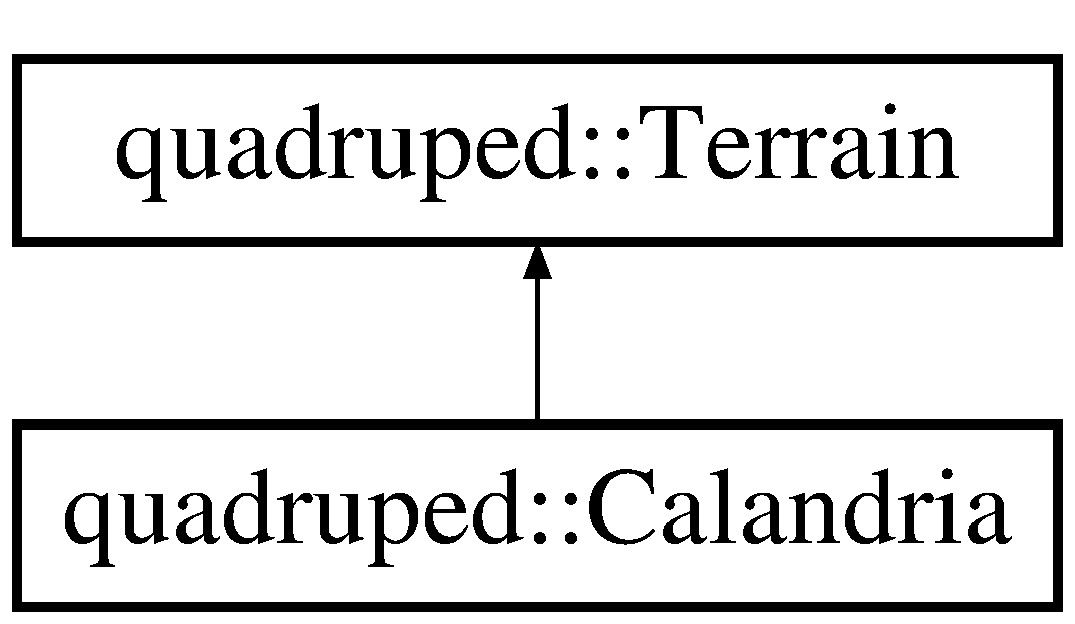
\includegraphics[height=2.000000cm]{classquadruped_1_1Calandria}
\end{center}
\end{figure}
\subsection*{Public 成员函数}
\begin{DoxyCompactItemize}
\item 
\mbox{\Hypertarget{classquadruped_1_1Calandria_abbc309b5641662f5879cb06dea7f6521}\label{classquadruped_1_1Calandria_abbc309b5641662f5879cb06dea7f6521}} 
\hyperlink{classquadruped_1_1Calandria_abbc309b5641662f5879cb06dea7f6521}{Calandria} (void)
\begin{DoxyCompactList}\small\item\em Calandria类的构造函数，完成地形标识符以及地形分割线的初始化 \end{DoxyCompactList}\item 
virtual double \hyperlink{classquadruped_1_1Calandria_ac2da35cda2dad19c9eb6c40a1e8c7a09}{Get\+Hight} (double p\+\_\+x, double p\+\_\+y) override
\begin{DoxyCompactList}\small\item\em 获取当前地形在世界坐标系下的高度 \end{DoxyCompactList}\item 
virtual void \hyperlink{classquadruped_1_1Calandria_abb0128d7dc204f91a728f6bb3f5a92e4}{Updata\+Edge} (double p\+\_\+first\+\_\+edge\+\_\+\+D\+\_\+x, double p\+\_\+first\+\_\+edge\+\_\+\+D\+\_\+y) override
\begin{DoxyCompactList}\small\item\em 获取每根排管轴线中点在世界坐标系下的位置以及分割线和危险区的设置 \end{DoxyCompactList}\item 
virtual \hyperlink{cppTypes_8h_a65c27bf97693676535dd0b30ea0ad399}{Vec3}$<$ double $>$ \hyperlink{classquadruped_1_1Calandria_ab2ed378cab5e226de452ed6a94fd1721}{Get\+Normal\+Vector} (double p\+\_\+x, double p\+\_\+y) override
\begin{DoxyCompactList}\small\item\em 预留接口 $\vert$ 获取排管某一点处的法向量 \end{DoxyCompactList}\end{DoxyCompactItemize}
\subsection*{额外继承的成员函数}


\subsection{详细描述}
排管类子类 

\subsection{成员函数说明}
\mbox{\Hypertarget{classquadruped_1_1Calandria_ac2da35cda2dad19c9eb6c40a1e8c7a09}\label{classquadruped_1_1Calandria_ac2da35cda2dad19c9eb6c40a1e8c7a09}} 
\index{quadruped\+::\+Calandria@{quadruped\+::\+Calandria}!Get\+Hight@{Get\+Hight}}
\index{Get\+Hight@{Get\+Hight}!quadruped\+::\+Calandria@{quadruped\+::\+Calandria}}
\subsubsection{\texorpdfstring{Get\+Hight()}{GetHight()}}
{\footnotesize\ttfamily double Calandria\+::\+Get\+Hight (\begin{DoxyParamCaption}\item[{double}]{p\+\_\+x,  }\item[{double}]{p\+\_\+y }\end{DoxyParamCaption})\hspace{0.3cm}{\ttfamily [override]}, {\ttfamily [virtual]}}



获取当前地形在世界坐标系下的高度 


\begin{DoxyParams}{参数}
{\em p\+\_\+x} & 当前点在世界坐标系位置坐标的\+X值 \\
\hline
{\em p\+\_\+y} & 当前点在世界坐标系位置坐标的\+Y值 \\
\hline
\end{DoxyParams}
\begin{DoxyReturn}{返回}
double 
\end{DoxyReturn}


重载 \hyperlink{classquadruped_1_1Terrain}{quadruped\+::\+Terrain} .

\mbox{\Hypertarget{classquadruped_1_1Calandria_ab2ed378cab5e226de452ed6a94fd1721}\label{classquadruped_1_1Calandria_ab2ed378cab5e226de452ed6a94fd1721}} 
\index{quadruped\+::\+Calandria@{quadruped\+::\+Calandria}!Get\+Normal\+Vector@{Get\+Normal\+Vector}}
\index{Get\+Normal\+Vector@{Get\+Normal\+Vector}!quadruped\+::\+Calandria@{quadruped\+::\+Calandria}}
\subsubsection{\texorpdfstring{Get\+Normal\+Vector()}{GetNormalVector()}}
{\footnotesize\ttfamily \hyperlink{cppTypes_8h_a65c27bf97693676535dd0b30ea0ad399}{Vec3}$<$ double $>$ Calandria\+::\+Get\+Normal\+Vector (\begin{DoxyParamCaption}\item[{double}]{p\+\_\+x,  }\item[{double}]{p\+\_\+y }\end{DoxyParamCaption})\hspace{0.3cm}{\ttfamily [override]}, {\ttfamily [virtual]}}



预留接口 $\vert$ 获取排管某一点处的法向量 


\begin{DoxyParams}{参数}
{\em p\+\_\+x} & \\
\hline
{\em p\+\_\+y} & \\
\hline
\end{DoxyParams}
\begin{DoxyReturn}{返回}
Vec3$<$double$>$ 
\end{DoxyReturn}


实现了 \hyperlink{classquadruped_1_1Terrain}{quadruped\+::\+Terrain}.

\mbox{\Hypertarget{classquadruped_1_1Calandria_abb0128d7dc204f91a728f6bb3f5a92e4}\label{classquadruped_1_1Calandria_abb0128d7dc204f91a728f6bb3f5a92e4}} 
\index{quadruped\+::\+Calandria@{quadruped\+::\+Calandria}!Updata\+Edge@{Updata\+Edge}}
\index{Updata\+Edge@{Updata\+Edge}!quadruped\+::\+Calandria@{quadruped\+::\+Calandria}}
\subsubsection{\texorpdfstring{Updata\+Edge()}{UpdataEdge()}}
{\footnotesize\ttfamily void Calandria\+::\+Updata\+Edge (\begin{DoxyParamCaption}\item[{double}]{p\+\_\+first\+\_\+edge\+\_\+\+D\+\_\+x,  }\item[{double}]{p\+\_\+first\+\_\+edge\+\_\+\+D\+\_\+y }\end{DoxyParamCaption})\hspace{0.3cm}{\ttfamily [override]}, {\ttfamily [virtual]}}



获取每根排管轴线中点在世界坐标系下的位置以及分割线和危险区的设置 


\begin{DoxyParams}{参数}
{\em p\+\_\+first\+\_\+edge\+\_\+\+D\+\_\+x} & 当前点在世界坐标系位置坐标的\+X值 \\
\hline
{\em p\+\_\+first\+\_\+edge\+\_\+\+D\+\_\+y} & 当前点在世界坐标系位置坐标的\+Y值 \\
\hline
\end{DoxyParams}


重载 \hyperlink{classquadruped_1_1Terrain}{quadruped\+::\+Terrain} .



参考 quadruped\+::\+Terrain\+::average\+Danger\+Area, C\+A\+L\+A\+N\+D\+R\+I\+A\+\_\+\+D\+I\+S\+T\+A\+N\+CE, quadruped\+::\+Terrain\+::first\+\_\+edge\+\_\+\+D\+\_\+x, quadruped\+::\+Terrain\+::first\+\_\+edge\+\_\+\+D\+\_\+y, L\+I\+M\+I\+T\+\_\+\+I\+N\+F\+I\+N\+I\+TE, quadruped\+::\+Terrain\+::num\+Split, quadruped\+::\+Terrain\+::safe\+Area , 以及 quadruped\+::\+Terrain\+::split.



该类的文档由以下文件生成\+:\begin{DoxyCompactItemize}
\item 
controller/motion\+Plan/terrain/\hyperlink{terrain_8hpp}{terrain.\+hpp}\item 
controller/motion\+Plan/terrain/\hyperlink{terrain_8cpp}{terrain.\+cpp}\end{DoxyCompactItemize}

\hypertarget{classquadruped_1_1Common}{}\section{quadruped\+:\+:Common类 参考}
\label{classquadruped_1_1Common}\index{quadruped\+::\+Common@{quadruped\+::\+Common}}


Actiger通用函数类  




{\ttfamily \#include $<$common\+Function.\+hpp$>$}

\subsection*{Public 成员函数}
\begin{DoxyCompactItemize}
\item 
\mbox{\Hypertarget{classquadruped_1_1Common_a238749d318a2208574129c4aa5477cda}\label{classquadruped_1_1Common_a238749d318a2208574129c4aa5477cda}} 
\hyperlink{classquadruped_1_1Common_a238749d318a2208574129c4aa5477cda}{Common} (void)
\begin{DoxyCompactList}\small\item\em Common类的构造函数 \end{DoxyCompactList}\item 
\mbox{\Hypertarget{classquadruped_1_1Common_ae5929aa0ce32558ecb76f9593d8e0e15}\label{classquadruped_1_1Common_ae5929aa0ce32558ecb76f9593d8e0e15}} 
virtual \hyperlink{classquadruped_1_1Common_ae5929aa0ce32558ecb76f9593d8e0e15}{$\sim$\+Common} (void)
\begin{DoxyCompactList}\small\item\em Common类的析构函数 \end{DoxyCompactList}\end{DoxyCompactItemize}
\subsection*{静态 Public 成员函数}
\begin{DoxyCompactItemize}
\item 
static \hyperlink{cppTypes_8h_adb7d462b35d31f0b2583b3e230a2a2c3}{Mat3}$<$ double $>$ \hyperlink{classquadruped_1_1Common_a471c7074d56b4a2c856ff21e680e67a8}{Rotation\+Matrix} (\hyperlink{cppTypes_8h_a65c27bf97693676535dd0b30ea0ad399}{Vec3}$<$ double $>$ p\+\_\+actul\+\_\+body\+\_\+angle)
\begin{DoxyCompactList}\small\item\em 构建三维旋转矩阵\mbox{[}World -\/$>$ Body $\vert$ roll + pitch + yaw\mbox{]} \end{DoxyCompactList}\item 
static \hyperlink{cppTypes_8h_adb7d462b35d31f0b2583b3e230a2a2c3}{Mat3}$<$ double $>$ \hyperlink{classquadruped_1_1Common_aa0a116c7c23dea6de2cd2dcd28b644b6}{Rotation\+Of\+Z\+Matrix} (double yaw)
\begin{DoxyCompactList}\small\item\em 构建三维旋转矩阵\mbox{[}World -\/$>$ Body $\vert$ yaw\mbox{]} \end{DoxyCompactList}\item 
static \hyperlink{cppTypes_8h_adb7d462b35d31f0b2583b3e230a2a2c3}{Mat3}$<$ double $>$ \hyperlink{classquadruped_1_1Common_a8b05a953662bcadd1cd3bf7dd17ae866}{Get\+Skew\+Symmetric\+Matrix} (\hyperlink{cppTypes_8h_a65c27bf97693676535dd0b30ea0ad399}{Vec3}$<$ double $>$ vector)
\begin{DoxyCompactList}\small\item\em 将向量转化为叉乘矩阵 \end{DoxyCompactList}\item 
static \hyperlink{cppTypes_8h_a5db6bfb25afa103db1fb6bb6287ae9d7}{D\+Mat}$<$ double $>$ \hyperlink{classquadruped_1_1Common_a972d5fc8430f5aa57706d0a7f0cc267e}{Pinv} (\hyperlink{cppTypes_8h_a5db6bfb25afa103db1fb6bb6287ae9d7}{D\+Mat}$<$ double $>$ matrix)
\begin{DoxyCompactList}\small\item\em 矩阵求伪逆 \end{DoxyCompactList}\item 
static \hyperlink{cppTypes_8h_a5db6bfb25afa103db1fb6bb6287ae9d7}{D\+Mat}$<$ double $>$ \hyperlink{classquadruped_1_1Common_a0b5411a1c977d54a3f2cf88ab7662c1c}{Weighted\+Inverse} (\hyperlink{cppTypes_8h_a5db6bfb25afa103db1fb6bb6287ae9d7}{D\+Mat}$<$ double $>$ J, \hyperlink{cppTypes_8h_a5db6bfb25afa103db1fb6bb6287ae9d7}{D\+Mat}$<$ double $>$ Winv)
\end{DoxyCompactItemize}


\subsection{详细描述}
Actiger通用函数类 

\subsection{成员函数说明}
\mbox{\Hypertarget{classquadruped_1_1Common_a8b05a953662bcadd1cd3bf7dd17ae866}\label{classquadruped_1_1Common_a8b05a953662bcadd1cd3bf7dd17ae866}} 
\index{quadruped\+::\+Common@{quadruped\+::\+Common}!Get\+Skew\+Symmetric\+Matrix@{Get\+Skew\+Symmetric\+Matrix}}
\index{Get\+Skew\+Symmetric\+Matrix@{Get\+Skew\+Symmetric\+Matrix}!quadruped\+::\+Common@{quadruped\+::\+Common}}
\subsubsection{\texorpdfstring{Get\+Skew\+Symmetric\+Matrix()}{GetSkewSymmetricMatrix()}}
{\footnotesize\ttfamily \hyperlink{cppTypes_8h_adb7d462b35d31f0b2583b3e230a2a2c3}{Mat3}$<$ double $>$ Common\+::\+Get\+Skew\+Symmetric\+Matrix (\begin{DoxyParamCaption}\item[{\hyperlink{cppTypes_8h_a65c27bf97693676535dd0b30ea0ad399}{Vec3}$<$ double $>$}]{vector }\end{DoxyParamCaption})\hspace{0.3cm}{\ttfamily [static]}}



将向量转化为叉乘矩阵 


\begin{DoxyParams}{参数}
{\em vector} & 待转化的向量 \\
\hline
\end{DoxyParams}
\begin{DoxyReturn}{返回}
Mat3$<$double$>$ 
\end{DoxyReturn}
\mbox{\Hypertarget{classquadruped_1_1Common_a972d5fc8430f5aa57706d0a7f0cc267e}\label{classquadruped_1_1Common_a972d5fc8430f5aa57706d0a7f0cc267e}} 
\index{quadruped\+::\+Common@{quadruped\+::\+Common}!Pinv@{Pinv}}
\index{Pinv@{Pinv}!quadruped\+::\+Common@{quadruped\+::\+Common}}
\subsubsection{\texorpdfstring{Pinv()}{Pinv()}}
{\footnotesize\ttfamily \hyperlink{cppTypes_8h_a5db6bfb25afa103db1fb6bb6287ae9d7}{D\+Mat}$<$ double $>$ Common\+::\+Pinv (\begin{DoxyParamCaption}\item[{\hyperlink{cppTypes_8h_a5db6bfb25afa103db1fb6bb6287ae9d7}{D\+Mat}$<$ double $>$}]{matrix }\end{DoxyParamCaption})\hspace{0.3cm}{\ttfamily [static]}}



矩阵求伪逆 


\begin{DoxyParams}{参数}
{\em matrix} & 待求伪逆矩阵 \\
\hline
\end{DoxyParams}
\begin{DoxyReturn}{返回}
D\+Mat$<$double$>$ 
\end{DoxyReturn}


参考自 Weighted\+Inverse().

\mbox{\Hypertarget{classquadruped_1_1Common_a471c7074d56b4a2c856ff21e680e67a8}\label{classquadruped_1_1Common_a471c7074d56b4a2c856ff21e680e67a8}} 
\index{quadruped\+::\+Common@{quadruped\+::\+Common}!Rotation\+Matrix@{Rotation\+Matrix}}
\index{Rotation\+Matrix@{Rotation\+Matrix}!quadruped\+::\+Common@{quadruped\+::\+Common}}
\subsubsection{\texorpdfstring{Rotation\+Matrix()}{RotationMatrix()}}
{\footnotesize\ttfamily \hyperlink{cppTypes_8h_adb7d462b35d31f0b2583b3e230a2a2c3}{Mat3}$<$ double $>$ Common\+::\+Rotation\+Matrix (\begin{DoxyParamCaption}\item[{\hyperlink{cppTypes_8h_a65c27bf97693676535dd0b30ea0ad399}{Vec3}$<$ double $>$}]{p\+\_\+actul\+\_\+body\+\_\+angle }\end{DoxyParamCaption})\hspace{0.3cm}{\ttfamily [static]}}



构建三维旋转矩阵\mbox{[}World -\/$>$ Body $\vert$ roll + pitch + yaw\mbox{]} 


\begin{DoxyParams}{参数}
{\em p\+\_\+actul\+\_\+body\+\_\+angle} & Actiger实际的欧拉角 \\
\hline
\end{DoxyParams}
\begin{DoxyReturn}{返回}
Mat3$<$double$>$ 
\end{DoxyReturn}


参考自 quadruped\+::\+Body\+State\+Estimate\+::$\sim$\+Body\+State\+Estimate().

\mbox{\Hypertarget{classquadruped_1_1Common_aa0a116c7c23dea6de2cd2dcd28b644b6}\label{classquadruped_1_1Common_aa0a116c7c23dea6de2cd2dcd28b644b6}} 
\index{quadruped\+::\+Common@{quadruped\+::\+Common}!Rotation\+Of\+Z\+Matrix@{Rotation\+Of\+Z\+Matrix}}
\index{Rotation\+Of\+Z\+Matrix@{Rotation\+Of\+Z\+Matrix}!quadruped\+::\+Common@{quadruped\+::\+Common}}
\subsubsection{\texorpdfstring{Rotation\+Of\+Z\+Matrix()}{RotationOfZMatrix()}}
{\footnotesize\ttfamily \hyperlink{cppTypes_8h_adb7d462b35d31f0b2583b3e230a2a2c3}{Mat3}$<$ double $>$ Common\+::\+Rotation\+Of\+Z\+Matrix (\begin{DoxyParamCaption}\item[{double}]{yaw }\end{DoxyParamCaption})\hspace{0.3cm}{\ttfamily [static]}}



构建三维旋转矩阵\mbox{[}World -\/$>$ Body $\vert$ yaw\mbox{]} 


\begin{DoxyParams}{参数}
{\em yaw} & Actiger实际的偏航角 \\
\hline
\end{DoxyParams}
\begin{DoxyReturn}{返回}
Mat3$<$double$>$ 
\end{DoxyReturn}


参考自 quadruped\+::\+F\+H\+\_\+constraints\+::\+Get\+Kinematics\+Cst() , 以及 quadruped\+::\+F\+H\+\_\+constraints\+::\+Get\+Other\+Cst().

\mbox{\Hypertarget{classquadruped_1_1Common_a0b5411a1c977d54a3f2cf88ab7662c1c}\label{classquadruped_1_1Common_a0b5411a1c977d54a3f2cf88ab7662c1c}} 
\index{quadruped\+::\+Common@{quadruped\+::\+Common}!Weighted\+Inverse@{Weighted\+Inverse}}
\index{Weighted\+Inverse@{Weighted\+Inverse}!quadruped\+::\+Common@{quadruped\+::\+Common}}
\subsubsection{\texorpdfstring{Weighted\+Inverse()}{WeightedInverse()}}
{\footnotesize\ttfamily \hyperlink{cppTypes_8h_a5db6bfb25afa103db1fb6bb6287ae9d7}{D\+Mat}$<$ double $>$ Common\+::\+Weighted\+Inverse (\begin{DoxyParamCaption}\item[{\hyperlink{cppTypes_8h_a5db6bfb25afa103db1fb6bb6287ae9d7}{D\+Mat}$<$ double $>$}]{J,  }\item[{\hyperlink{cppTypes_8h_a5db6bfb25afa103db1fb6bb6287ae9d7}{D\+Mat}$<$ double $>$}]{Winv }\end{DoxyParamCaption})\hspace{0.3cm}{\ttfamily [static]}}


\begin{DoxyParams}{参数}
{\em J} & \\
\hline
{\em Winv} & \\
\hline
\end{DoxyParams}
\begin{DoxyReturn}{返回}
D\+Mat$<$double$>$ 
\end{DoxyReturn}


参考 Pinv().



该类的文档由以下文件生成\+:\begin{DoxyCompactItemize}
\item 
\hyperlink{commonFunction_8hpp}{common\+Function.\+hpp}\item 
\hyperlink{commonFunction_8cpp}{common\+Function.\+cpp}\end{DoxyCompactItemize}

\hypertarget{classquadruped_1_1ContactSpec}{}\section{quadruped\+:\+:Contact\+Spec类 参考}
\label{classquadruped_1_1ContactSpec}\index{quadruped\+::\+Contact\+Spec@{quadruped\+::\+Contact\+Spec}}
类 quadruped\+:\+:Contact\+Spec 继承关系图\+:\begin{figure}[H]
\begin{center}
\leavevmode
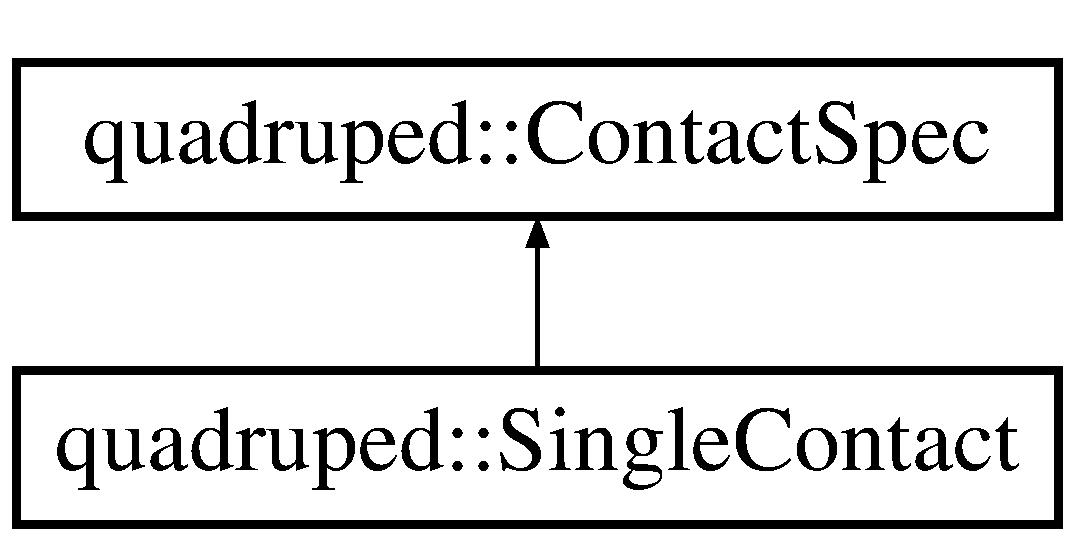
\includegraphics[height=2.000000cm]{classquadruped_1_1ContactSpec}
\end{center}
\end{figure}
\subsection*{Public 成员函数}
\begin{DoxyCompactItemize}
\item 
\mbox{\Hypertarget{classquadruped_1_1ContactSpec_a52d0ea89100165311779ff5dd1a823b8}\label{classquadruped_1_1ContactSpec_a52d0ea89100165311779ff5dd1a823b8}} 
{\bfseries Contact\+Spec} (size\+\_\+t dim)
\item 
\mbox{\Hypertarget{classquadruped_1_1ContactSpec_af5fe0d0de2a9d90ac49a68edf7b3f5f2}\label{classquadruped_1_1ContactSpec_af5fe0d0de2a9d90ac49a68edf7b3f5f2}} 
size\+\_\+t {\bfseries Get\+Dim} () const
\item 
\mbox{\Hypertarget{classquadruped_1_1ContactSpec_a2c038eac35cdc914324bd8cb08350070}\label{classquadruped_1_1ContactSpec_a2c038eac35cdc914324bd8cb08350070}} 
size\+\_\+t {\bfseries Get\+Dim\+R\+F\+Constraint} () const
\item 
\mbox{\Hypertarget{classquadruped_1_1ContactSpec_aab988347d4c0e03e5b895217443bc532}\label{classquadruped_1_1ContactSpec_aab988347d4c0e03e5b895217443bc532}} 
size\+\_\+t {\bfseries Get\+Fz\+Index} () const
\item 
\mbox{\Hypertarget{classquadruped_1_1ContactSpec_a16b839539ecbcf18a66f5b543e17547d}\label{classquadruped_1_1ContactSpec_a16b839539ecbcf18a66f5b543e17547d}} 
\hyperlink{cppTypes_8h_a5db6bfb25afa103db1fb6bb6287ae9d7}{D\+Mat}$<$ double $>$ {\bfseries Get\+Contact\+Jacobian} ()
\item 
\mbox{\Hypertarget{classquadruped_1_1ContactSpec_a23807f57318edb43222eee1755d05fe0}\label{classquadruped_1_1ContactSpec_a23807f57318edb43222eee1755d05fe0}} 
\hyperlink{cppTypes_8h_adad69baca3c77d5f991be5d3c063fea7}{D\+Vec}$<$ double $>$ {\bfseries Get\+Jc\+Dot\+Qdot} ()
\item 
\mbox{\Hypertarget{classquadruped_1_1ContactSpec_aa94bc7a970b7d76bb4ff19a7e557e2ea}\label{classquadruped_1_1ContactSpec_aa94bc7a970b7d76bb4ff19a7e557e2ea}} 
void {\bfseries Unset\+Contact} ()
\item 
\mbox{\Hypertarget{classquadruped_1_1ContactSpec_a82da6eaf26cb1cb6e49529d955aa17c6}\label{classquadruped_1_1ContactSpec_a82da6eaf26cb1cb6e49529d955aa17c6}} 
\hyperlink{cppTypes_8h_a5db6bfb25afa103db1fb6bb6287ae9d7}{D\+Mat}$<$ double $>$ {\bfseries Get\+R\+F\+Constraint\+Mtx} ()
\item 
\mbox{\Hypertarget{classquadruped_1_1ContactSpec_a2426023351e7a1caac03418335a91c20}\label{classquadruped_1_1ContactSpec_a2426023351e7a1caac03418335a91c20}} 
\hyperlink{cppTypes_8h_a5db6bfb25afa103db1fb6bb6287ae9d7}{D\+Mat}$<$ double $>$ {\bfseries Get\+R\+F\+Constraint\+VecL} ()
\item 
\mbox{\Hypertarget{classquadruped_1_1ContactSpec_ae668499ca7c34a8b950f58f45d4ad46f}\label{classquadruped_1_1ContactSpec_ae668499ca7c34a8b950f58f45d4ad46f}} 
\hyperlink{cppTypes_8h_a5db6bfb25afa103db1fb6bb6287ae9d7}{D\+Mat}$<$ double $>$ {\bfseries Get\+R\+F\+Constraint\+VecU} ()
\item 
\mbox{\Hypertarget{classquadruped_1_1ContactSpec_aec2ef05980f997148235386ae649510c}\label{classquadruped_1_1ContactSpec_aec2ef05980f997148235386ae649510c}} 
\hyperlink{cppTypes_8h_adad69baca3c77d5f991be5d3c063fea7}{D\+Vec}$<$ double $>$ {\bfseries Get\+R\+F\+Desired} ()
\item 
\mbox{\Hypertarget{classquadruped_1_1ContactSpec_a2f393f9d8a2fe2cadb9eb80a3d16aa44}\label{classquadruped_1_1ContactSpec_a2f393f9d8a2fe2cadb9eb80a3d16aa44}} 
void {\bfseries Set\+R\+F\+Desired} (\hyperlink{cppTypes_8h_adad69baca3c77d5f991be5d3c063fea7}{D\+Vec}$<$ double $>$ p\+\_\+fr\+\_\+des)
\item 
\mbox{\Hypertarget{classquadruped_1_1ContactSpec_a80906be5d63dd6b118e7ac5363989902}\label{classquadruped_1_1ContactSpec_a80906be5d63dd6b118e7ac5363989902}} 
bool {\bfseries Update\+Contact\+Spec} ()
\end{DoxyCompactItemize}
\subsection*{Protected 成员函数}
\begin{DoxyCompactItemize}
\item 
\mbox{\Hypertarget{classquadruped_1_1ContactSpec_afb40142b1239dde30c41ed44df0cd187}\label{classquadruped_1_1ContactSpec_afb40142b1239dde30c41ed44df0cd187}} 
virtual bool {\bfseries Update\+Jc} ()=0
\item 
\mbox{\Hypertarget{classquadruped_1_1ContactSpec_af7930d5409ea0c4e6de5ab7c8f3b1bed}\label{classquadruped_1_1ContactSpec_af7930d5409ea0c4e6de5ab7c8f3b1bed}} 
virtual bool {\bfseries Update\+Jc\+Dot\+Qdot} ()=0
\item 
\mbox{\Hypertarget{classquadruped_1_1ContactSpec_a4ad0b239265a6c6b84baa072792bb448}\label{classquadruped_1_1ContactSpec_a4ad0b239265a6c6b84baa072792bb448}} 
virtual bool {\bfseries Update\+Uf} ()=0
\item 
\mbox{\Hypertarget{classquadruped_1_1ContactSpec_a6d822adbe56fcd0f91d76dec7665f739}\label{classquadruped_1_1ContactSpec_a6d822adbe56fcd0f91d76dec7665f739}} 
virtual bool {\bfseries Update\+Inequality\+Vector} ()=0
\end{DoxyCompactItemize}
\subsection*{Protected 属性}
\begin{DoxyCompactItemize}
\item 
\mbox{\Hypertarget{classquadruped_1_1ContactSpec_a46f4198671400c78b21a799dde489331}\label{classquadruped_1_1ContactSpec_a46f4198671400c78b21a799dde489331}} 
int {\bfseries idx\+\_\+\+Fz}
\item 
\mbox{\Hypertarget{classquadruped_1_1ContactSpec_a62517e2badfa84581be15f68a96bbfc6}\label{classquadruped_1_1ContactSpec_a62517e2badfa84581be15f68a96bbfc6}} 
\hyperlink{cppTypes_8h_a5db6bfb25afa103db1fb6bb6287ae9d7}{D\+Mat}$<$ double $>$ {\bfseries cstr\+Mtx}
\item 
\mbox{\Hypertarget{classquadruped_1_1ContactSpec_aba1db003e83e2f4ab7bf41663ac9dc39}\label{classquadruped_1_1ContactSpec_aba1db003e83e2f4ab7bf41663ac9dc39}} 
\hyperlink{cppTypes_8h_adad69baca3c77d5f991be5d3c063fea7}{D\+Vec}$<$ double $>$ {\bfseries fr\+\_\+des}
\item 
\mbox{\Hypertarget{classquadruped_1_1ContactSpec_ae22e8b5d4acb18fac83978d890c06360}\label{classquadruped_1_1ContactSpec_ae22e8b5d4acb18fac83978d890c06360}} 
\hyperlink{cppTypes_8h_adad69baca3c77d5f991be5d3c063fea7}{D\+Vec}$<$ double $>$ {\bfseries ieq\+\_\+vec\+\_\+l}
\item 
\mbox{\Hypertarget{classquadruped_1_1ContactSpec_a1525ed349c50498bcc0fa1e85e4b097a}\label{classquadruped_1_1ContactSpec_a1525ed349c50498bcc0fa1e85e4b097a}} 
\hyperlink{cppTypes_8h_adad69baca3c77d5f991be5d3c063fea7}{D\+Vec}$<$ double $>$ {\bfseries ieq\+\_\+vec\+\_\+u}
\item 
\mbox{\Hypertarget{classquadruped_1_1ContactSpec_a22d932b636b12b1db0958a373a84f03f}\label{classquadruped_1_1ContactSpec_a22d932b636b12b1db0958a373a84f03f}} 
\hyperlink{cppTypes_8h_a6e18c50269e5924351437a22db0e9840}{Mat3x18}$<$ double $>$ {\bfseries Jc}
\item 
\mbox{\Hypertarget{classquadruped_1_1ContactSpec_a418193cad65a2e2b61f4072ae81aa695}\label{classquadruped_1_1ContactSpec_a418193cad65a2e2b61f4072ae81aa695}} 
\hyperlink{cppTypes_8h_adad69baca3c77d5f991be5d3c063fea7}{D\+Vec}$<$ double $>$ {\bfseries Jc\+Dot\+Qdot}
\item 
\mbox{\Hypertarget{classquadruped_1_1ContactSpec_a974b13c1ea9d232fe32787ebccc911fe}\label{classquadruped_1_1ContactSpec_a974b13c1ea9d232fe32787ebccc911fe}} 
size\+\_\+t {\bfseries dim\+\_\+contact}
\item 
\mbox{\Hypertarget{classquadruped_1_1ContactSpec_a664961f667c97bd5e759012de200a72c}\label{classquadruped_1_1ContactSpec_a664961f667c97bd5e759012de200a72c}} 
bool {\bfseries b\+\_\+set\+\_\+contact}
\end{DoxyCompactItemize}


该类的文档由以下文件生成\+:\begin{DoxyCompactItemize}
\item 
controller/wbc/contact/contact\+Spec.\+hpp\end{DoxyCompactItemize}

\hypertarget{classquadruped_1_1DynModel}{}\section{quadruped\+:\+:Dyn\+Model类 参考}
\label{classquadruped_1_1DynModel}\index{quadruped\+::\+Dyn\+Model@{quadruped\+::\+Dyn\+Model}}
\subsection*{Public 成员函数}
\begin{DoxyCompactItemize}
\item 
\mbox{\Hypertarget{classquadruped_1_1DynModel_ab672659353b9fc396875c4bbfed6d74e}\label{classquadruped_1_1DynModel_ab672659353b9fc396875c4bbfed6d74e}} 
{\bfseries Dyn\+Model} (Rigid\+Body\+Dynamics\+::\+Model $\ast$model)
\item 
\mbox{\Hypertarget{classquadruped_1_1DynModel_abfc19642bbacc9832a609538b30470fc}\label{classquadruped_1_1DynModel_abfc19642bbacc9832a609538b30470fc}} 
bool {\bfseries get\+Mass\+Inertia} (dynacore\+::\+Matrix \&a)
\item 
\mbox{\Hypertarget{classquadruped_1_1DynModel_a104e7f42acd13041c6461f36255d6469}\label{classquadruped_1_1DynModel_a104e7f42acd13041c6461f36255d6469}} 
bool {\bfseries get\+Inverse\+Mass\+Inertia} (dynacore\+::\+Matrix \&ainv)
\item 
\mbox{\Hypertarget{classquadruped_1_1DynModel_a9936433050d9bf75c60e093aab1ae405}\label{classquadruped_1_1DynModel_a9936433050d9bf75c60e093aab1ae405}} 
bool {\bfseries get\+Gravity} (dynacore\+::\+Vector \&grav)
\item 
\mbox{\Hypertarget{classquadruped_1_1DynModel_a21c4d63ca3fe7a1f90993ec90ba0a2c8}\label{classquadruped_1_1DynModel_a21c4d63ca3fe7a1f90993ec90ba0a2c8}} 
bool {\bfseries get\+Coriolis} (dynacore\+::\+Vector \&coriolis)
\item 
\mbox{\Hypertarget{classquadruped_1_1DynModel_a023e8a5a6480a2c025e8d1e58c2175df}\label{classquadruped_1_1DynModel_a023e8a5a6480a2c025e8d1e58c2175df}} 
void {\bfseries Update\+Dynamics} (const dynacore\+::\+Vector \&q, const dynacore\+::\+Vector \&qdot)
\end{DoxyCompactItemize}
\subsection*{Protected 属性}
\begin{DoxyCompactItemize}
\item 
\mbox{\Hypertarget{classquadruped_1_1DynModel_a56f317b42dd8ca721c8723f573018e80}\label{classquadruped_1_1DynModel_a56f317b42dd8ca721c8723f573018e80}} 
dynacore\+::\+Matrix {\bfseries A\+\_\+}
\item 
\mbox{\Hypertarget{classquadruped_1_1DynModel_a0d961539f3e26444b0064d9d286b0dd8}\label{classquadruped_1_1DynModel_a0d961539f3e26444b0064d9d286b0dd8}} 
dynacore\+::\+Matrix {\bfseries Ainv\+\_\+}
\item 
\mbox{\Hypertarget{classquadruped_1_1DynModel_a4cc208318b72f683f7dd5097d4a3c8da}\label{classquadruped_1_1DynModel_a4cc208318b72f683f7dd5097d4a3c8da}} 
dynacore\+::\+Vector {\bfseries grav\+\_\+}
\item 
\mbox{\Hypertarget{classquadruped_1_1DynModel_a8e200c399836e1db3e3d8b0b8ba738da}\label{classquadruped_1_1DynModel_a8e200c399836e1db3e3d8b0b8ba738da}} 
dynacore\+::\+Vector {\bfseries coriolis\+\_\+}
\item 
\mbox{\Hypertarget{classquadruped_1_1DynModel_ab4eac018b2b0385acbd30351c0594d29}\label{classquadruped_1_1DynModel_ab4eac018b2b0385acbd30351c0594d29}} 
Rigid\+Body\+Dynamics\+::\+Model $\ast$ {\bfseries model\+\_\+}
\end{DoxyCompactItemize}


该类的文档由以下文件生成\+:\begin{DoxyCompactItemize}
\item 
controller/model/Dyn\+Model.\+hpp\item 
controller/model/Dyn\+Model.\+cpp\end{DoxyCompactItemize}

\hypertarget{classquadruped_1_1DynWBC}{}\section{quadruped\+:\+:Dyn\+W\+B\+C类 参考}
\label{classquadruped_1_1DynWBC}\index{quadruped\+::\+Dyn\+W\+BC@{quadruped\+::\+Dyn\+W\+BC}}
\subsection*{Public 成员函数}
\begin{DoxyCompactItemize}
\item 
\mbox{\Hypertarget{classquadruped_1_1DynWBC_a45addb67f275b705bdd91653ed3e3b8d}\label{classquadruped_1_1DynWBC_a45addb67f275b705bdd91653ed3e3b8d}} 
{\bfseries Dyn\+W\+BC} (size\+\_\+t p\+\_\+num\+\_\+qdot, const std\+::vector$<$ \hyperlink{classquadruped_1_1ContactSpec}{Contact\+Spec} $\ast$$>$ $\ast$p\+\_\+contact\+\_\+list, const std\+::vector$<$ \hyperlink{classquadruped_1_1Task}{Task} $\ast$$>$ $\ast$p\+\_\+task\+\_\+list)
\item 
\mbox{\Hypertarget{classquadruped_1_1DynWBC_a28c18329b95f92bc3c88dff477902f13}\label{classquadruped_1_1DynWBC_a28c18329b95f92bc3c88dff477902f13}} 
\hyperlink{cppTypes_8h_adad69baca3c77d5f991be5d3c063fea7}{D\+Vec}$<$ double $>$ {\bfseries Make\+Torque} (void)
\item 
\mbox{\Hypertarget{classquadruped_1_1DynWBC_ab4228b91b88daf062fdde0b21afe69b2}\label{classquadruped_1_1DynWBC_ab4228b91b88daf062fdde0b21afe69b2}} 
void {\bfseries Update\+Setting} (const \hyperlink{cppTypes_8h_a5db6bfb25afa103db1fb6bb6287ae9d7}{D\+Mat}$<$ double $>$ \&p\+\_\+A, const \hyperlink{cppTypes_8h_a5db6bfb25afa103db1fb6bb6287ae9d7}{D\+Mat}$<$ double $>$ \&p\+\_\+\+Ainv, const \hyperlink{cppTypes_8h_adad69baca3c77d5f991be5d3c063fea7}{D\+Vec}$<$ double $>$ \&p\+\_\+cori, const \hyperlink{cppTypes_8h_adad69baca3c77d5f991be5d3c063fea7}{D\+Vec}$<$ double $>$ \&p\+\_\+grav)
\end{DoxyCompactItemize}
\subsection*{Public 属性}
\begin{DoxyCompactItemize}
\item 
\mbox{\Hypertarget{classquadruped_1_1DynWBC_a9a04ee0db872de798abe7cb3f571eaa5}\label{classquadruped_1_1DynWBC_a9a04ee0db872de798abe7cb3f571eaa5}} 
\hyperlink{cppTypes_8h_a5db6bfb25afa103db1fb6bb6287ae9d7}{D\+Mat}$<$ double $>$ {\bfseries w\+\_\+floating}
\item 
\mbox{\Hypertarget{classquadruped_1_1DynWBC_a9d09d5faede19d842e5a17da328e4e23}\label{classquadruped_1_1DynWBC_a9d09d5faede19d842e5a17da328e4e23}} 
\hyperlink{cppTypes_8h_a5db6bfb25afa103db1fb6bb6287ae9d7}{D\+Mat}$<$ double $>$ {\bfseries w\+\_\+rf}
\item 
\mbox{\Hypertarget{classquadruped_1_1DynWBC_a1e5ae78991b3214d3774f0d5422210d7}\label{classquadruped_1_1DynWBC_a1e5ae78991b3214d3774f0d5422210d7}} 
const std\+::vector$<$ \hyperlink{classquadruped_1_1ContactSpec}{Contact\+Spec} $\ast$ $>$ $\ast$ {\bfseries contact\+\_\+list}
\item 
\mbox{\Hypertarget{classquadruped_1_1DynWBC_a06fff363979f875745569e1edc7e3367}\label{classquadruped_1_1DynWBC_a06fff363979f875745569e1edc7e3367}} 
const std\+::vector$<$ \hyperlink{classquadruped_1_1Task}{Task} $\ast$ $>$ $\ast$ {\bfseries task\+\_\+list}
\end{DoxyCompactItemize}


该类的文档由以下文件生成\+:\begin{DoxyCompactItemize}
\item 
controller/wbc/\+W\+B\+I\+C/dyn\+W\+B\+C.\+hpp\item 
controller/wbc/\+W\+B\+I\+C/\hyperlink{dynWBC_8cpp}{dyn\+W\+B\+C.\+cpp}\end{DoxyCompactItemize}

\hypertarget{classquadruped_1_1EndfootTrajectory}{}\section{quadruped\+:\+:Endfoot\+Trajectory类 参考}
\label{classquadruped_1_1EndfootTrajectory}\index{quadruped\+::\+Endfoot\+Trajectory@{quadruped\+::\+Endfoot\+Trajectory}}
\subsection*{Public 成员函数}
\begin{DoxyCompactItemize}
\item 
\mbox{\Hypertarget{classquadruped_1_1EndfootTrajectory_a4163640cae45e8c3dedd6869c3c1eff6}\label{classquadruped_1_1EndfootTrajectory_a4163640cae45e8c3dedd6869c3c1eff6}} 
{\bfseries Endfoot\+Trajectory} (\hyperlink{classquadruped_1_1Parameters}{Parameters} $\ast$p\+\_\+para, \hyperlink{classquadruped_1_1Terrain}{Terrain} $\ast$p\+\_\+terrain\+\_\+now)
\item 
\mbox{\Hypertarget{classquadruped_1_1EndfootTrajectory_a87bfadf8ed778c1b6a9a23225da0f080}\label{classquadruped_1_1EndfootTrajectory_a87bfadf8ed778c1b6a9a23225da0f080}} 
double {\bfseries Calcu\+OvalX} (double p\+\_\+z, \hyperlink{structoval__t}{oval\+\_\+t} p\+\_\+oval)
\item 
\mbox{\Hypertarget{classquadruped_1_1EndfootTrajectory_a0701c295f3a4e8c9df697255f69d1cc8}\label{classquadruped_1_1EndfootTrajectory_a0701c295f3a4e8c9df697255f69d1cc8}} 
double {\bfseries Calcu\+OvalZ} (double p\+\_\+x, \hyperlink{structoval__t}{oval\+\_\+t} p\+\_\+oval)
\item 
double \hyperlink{classquadruped_1_1EndfootTrajectory_ae5ae8428e6a555fbcd5b1fb212966821}{Get\+OvalB} (double pointX, double pointZ, \hyperlink{structoval__t}{oval\+\_\+t} oval)
\item 
void \hyperlink{classquadruped_1_1EndfootTrajectory_afd7f3ba204c58ec5cb23b0a3e09e269d}{Get\+Oval\+Fuction} (\hyperlink{cppTypes_8h_a65c27bf97693676535dd0b30ea0ad399}{Vec3}$<$ double $>$ start\+Point, \hyperlink{cppTypes_8h_a65c27bf97693676535dd0b30ea0ad399}{Vec3}$<$ double $>$ end\+Point, \hyperlink{cppTypes_8h_a65c27bf97693676535dd0b30ea0ad399}{Vec3}$<$ double $>$ another\+Point, \hyperlink{structoval__t}{oval\+\_\+t} $\ast$ovall)
\begin{DoxyCompactList}\small\item\em 构建\+Actiger摆动腿足端轨迹方程 \end{DoxyCompactList}\item 
\mbox{\Hypertarget{classquadruped_1_1EndfootTrajectory_a8efd46aefe9b2a959d8ea8944c437db7}\label{classquadruped_1_1EndfootTrajectory_a8efd46aefe9b2a959d8ea8944c437db7}} 
void {\bfseries Get\+Beeline\+Fuction} (\hyperlink{cppTypes_8h_a65c27bf97693676535dd0b30ea0ad399}{Vec3}$<$ double $>$ start\+Point, \hyperlink{cppTypes_8h_a65c27bf97693676535dd0b30ea0ad399}{Vec3}$<$ double $>$ end\+Point, \hyperlink{structbeeline__t}{beeline\+\_\+t} $\ast$beeline)
\item 
\mbox{\Hypertarget{classquadruped_1_1EndfootTrajectory_ad2728987b4fee1ef4f234ce8c8faad73}\label{classquadruped_1_1EndfootTrajectory_ad2728987b4fee1ef4f234ce8c8faad73}} 
\hyperlink{cppTypes_8h_a65c27bf97693676535dd0b30ea0ad399}{Vec3}$<$ double $>$ {\bfseries Select\+Another\+Point} (\hyperlink{cppTypes_8h_a65c27bf97693676535dd0b30ea0ad399}{Vec3}$<$ double $>$ start\+Point, \hyperlink{cppTypes_8h_a65c27bf97693676535dd0b30ea0ad399}{Vec3}$<$ double $>$ end\+Point)
\item 
void \hyperlink{classquadruped_1_1EndfootTrajectory_a1fa9a93f47cd777141b592f461218865}{Get\+Endfoot\+Trajectory} (int p\+\_\+grid, \hyperlink{cppTypes_8h_a65c27bf97693676535dd0b30ea0ad399}{Vec3}$<$ double $>$ p\+\_\+front\+\_\+start\+Point, \hyperlink{cppTypes_8h_a65c27bf97693676535dd0b30ea0ad399}{Vec3}$<$ double $>$ p\+\_\+rear\+\_\+start\+Point, \hyperlink{cppTypes_8h_a65c27bf97693676535dd0b30ea0ad399}{Vec3}$<$ double $>$ p\+\_\+front\+\_\+end\+Point, \hyperlink{cppTypes_8h_a65c27bf97693676535dd0b30ea0ad399}{Vec3}$<$ double $>$ p\+\_\+rear\+\_\+end\+Point, \hyperlink{cppTypes_8h_a5db6bfb25afa103db1fb6bb6287ae9d7}{D\+Mat}$<$ double $>$ p\+\_\+spatial\+\_\+list)
\begin{DoxyCompactList}\small\item\em 获取摆动腿足端轨迹 \end{DoxyCompactList}\end{DoxyCompactItemize}
\subsection*{Public 属性}
\begin{DoxyCompactItemize}
\item 
\mbox{\Hypertarget{classquadruped_1_1EndfootTrajectory_ade502af2e3ace368246480dd23402e8e}\label{classquadruped_1_1EndfootTrajectory_ade502af2e3ace368246480dd23402e8e}} 
int {\bfseries grid}
\item 
\mbox{\Hypertarget{classquadruped_1_1EndfootTrajectory_a9f51d4eeb6d666f4e8fb9d876451b1fc}\label{classquadruped_1_1EndfootTrajectory_a9f51d4eeb6d666f4e8fb9d876451b1fc}} 
\hyperlink{structoval__t}{oval\+\_\+t} {\bfseries front\+Oval} =\{0\}
\item 
\mbox{\Hypertarget{classquadruped_1_1EndfootTrajectory_a267a97a8f91ad125d2830057015aa57a}\label{classquadruped_1_1EndfootTrajectory_a267a97a8f91ad125d2830057015aa57a}} 
\hyperlink{structoval__t}{oval\+\_\+t} {\bfseries rear\+Oval} =\{0\}
\item 
\mbox{\Hypertarget{classquadruped_1_1EndfootTrajectory_aa6daa3b91d35e3fc8d57fd2f48db6384}\label{classquadruped_1_1EndfootTrajectory_aa6daa3b91d35e3fc8d57fd2f48db6384}} 
double {\bfseries height}
\item 
\mbox{\Hypertarget{classquadruped_1_1EndfootTrajectory_a40ef1a8b6ca2b1d823e316824c202324}\label{classquadruped_1_1EndfootTrajectory_a40ef1a8b6ca2b1d823e316824c202324}} 
\hyperlink{classquadruped_1_1Terrain}{Terrain} $\ast$ {\bfseries terrain\+\_\+now}
\item 
\mbox{\Hypertarget{classquadruped_1_1EndfootTrajectory_a80317eb8170d41eb95be495dc016b24c}\label{classquadruped_1_1EndfootTrajectory_a80317eb8170d41eb95be495dc016b24c}} 
\hyperlink{cppTypes_8h_a65c27bf97693676535dd0b30ea0ad399}{Vec3}$<$ double $>$ {\bfseries front\+\_\+start\+Point}
\item 
\mbox{\Hypertarget{classquadruped_1_1EndfootTrajectory_a724bfaedd5236538228beb0fef75fdb5}\label{classquadruped_1_1EndfootTrajectory_a724bfaedd5236538228beb0fef75fdb5}} 
\hyperlink{cppTypes_8h_a65c27bf97693676535dd0b30ea0ad399}{Vec3}$<$ double $>$ {\bfseries front\+\_\+end\+Point}
\item 
\mbox{\Hypertarget{classquadruped_1_1EndfootTrajectory_ae48f247a0ff54fc6b4c8616b73264cd1}\label{classquadruped_1_1EndfootTrajectory_ae48f247a0ff54fc6b4c8616b73264cd1}} 
\hyperlink{cppTypes_8h_a65c27bf97693676535dd0b30ea0ad399}{Vec3}$<$ double $>$ {\bfseries front\+\_\+middle\+Point}
\item 
\mbox{\Hypertarget{classquadruped_1_1EndfootTrajectory_a32dd6be5dea4d14d64e90bad3423d291}\label{classquadruped_1_1EndfootTrajectory_a32dd6be5dea4d14d64e90bad3423d291}} 
\hyperlink{cppTypes_8h_a65c27bf97693676535dd0b30ea0ad399}{Vec3}$<$ double $>$ {\bfseries rear\+\_\+start\+Point}
\item 
\mbox{\Hypertarget{classquadruped_1_1EndfootTrajectory_ae5799b6b24ac0d12d22d650af700b88e}\label{classquadruped_1_1EndfootTrajectory_ae5799b6b24ac0d12d22d650af700b88e}} 
\hyperlink{cppTypes_8h_a65c27bf97693676535dd0b30ea0ad399}{Vec3}$<$ double $>$ {\bfseries rear\+\_\+end\+Point}
\item 
\mbox{\Hypertarget{classquadruped_1_1EndfootTrajectory_a27af70ef6d4ef5ff79fe74796554555a}\label{classquadruped_1_1EndfootTrajectory_a27af70ef6d4ef5ff79fe74796554555a}} 
\hyperlink{cppTypes_8h_a65c27bf97693676535dd0b30ea0ad399}{Vec3}$<$ double $>$ {\bfseries rear\+\_\+middle\+Point}
\item 
\mbox{\Hypertarget{classquadruped_1_1EndfootTrajectory_afe0b09fe7aa5420f86071480a6145cab}\label{classquadruped_1_1EndfootTrajectory_afe0b09fe7aa5420f86071480a6145cab}} 
\hyperlink{cppTypes_8h_a5db6bfb25afa103db1fb6bb6287ae9d7}{D\+Mat}$<$ double $>$ {\bfseries body\+\_\+spatial}
\item 
\mbox{\Hypertarget{classquadruped_1_1EndfootTrajectory_aa70aacd0bf618d1d5718ff716f3e609f}\label{classquadruped_1_1EndfootTrajectory_aa70aacd0bf618d1d5718ff716f3e609f}} 
\hyperlink{cppTypes_8h_a5db6bfb25afa103db1fb6bb6287ae9d7}{D\+Mat}$<$ double $>$ {\bfseries endfoot\+\_\+pos\+\_\+front\+\_\+list}
\item 
\mbox{\Hypertarget{classquadruped_1_1EndfootTrajectory_ab429ec6f45de88f6f735cc202dba6fee}\label{classquadruped_1_1EndfootTrajectory_ab429ec6f45de88f6f735cc202dba6fee}} 
\hyperlink{cppTypes_8h_a5db6bfb25afa103db1fb6bb6287ae9d7}{D\+Mat}$<$ double $>$ {\bfseries endfoot\+\_\+vel\+\_\+front\+\_\+list}
\item 
\mbox{\Hypertarget{classquadruped_1_1EndfootTrajectory_a13e802c72a0201a9008b2694d40a8ab1}\label{classquadruped_1_1EndfootTrajectory_a13e802c72a0201a9008b2694d40a8ab1}} 
\hyperlink{cppTypes_8h_a5db6bfb25afa103db1fb6bb6287ae9d7}{D\+Mat}$<$ double $>$ {\bfseries endfoot\+\_\+pos\+\_\+rear\+\_\+list}
\item 
\mbox{\Hypertarget{classquadruped_1_1EndfootTrajectory_a1f19d84b9d57dd20b252cdc82773a94a}\label{classquadruped_1_1EndfootTrajectory_a1f19d84b9d57dd20b252cdc82773a94a}} 
\hyperlink{cppTypes_8h_a5db6bfb25afa103db1fb6bb6287ae9d7}{D\+Mat}$<$ double $>$ {\bfseries endfoot\+\_\+vel\+\_\+rear\+\_\+list}
\end{DoxyCompactItemize}


\subsection{成员函数说明}
\mbox{\Hypertarget{classquadruped_1_1EndfootTrajectory_a1fa9a93f47cd777141b592f461218865}\label{classquadruped_1_1EndfootTrajectory_a1fa9a93f47cd777141b592f461218865}} 
\index{quadruped\+::\+Endfoot\+Trajectory@{quadruped\+::\+Endfoot\+Trajectory}!Get\+Endfoot\+Trajectory@{Get\+Endfoot\+Trajectory}}
\index{Get\+Endfoot\+Trajectory@{Get\+Endfoot\+Trajectory}!quadruped\+::\+Endfoot\+Trajectory@{quadruped\+::\+Endfoot\+Trajectory}}
\subsubsection{\texorpdfstring{Get\+Endfoot\+Trajectory()}{GetEndfootTrajectory()}}
{\footnotesize\ttfamily void Endfoot\+Trajectory\+::\+Get\+Endfoot\+Trajectory (\begin{DoxyParamCaption}\item[{int}]{p\+\_\+grid,  }\item[{\hyperlink{cppTypes_8h_a65c27bf97693676535dd0b30ea0ad399}{Vec3}$<$ double $>$}]{p\+\_\+front\+\_\+start\+Point,  }\item[{\hyperlink{cppTypes_8h_a65c27bf97693676535dd0b30ea0ad399}{Vec3}$<$ double $>$}]{p\+\_\+rear\+\_\+start\+Point,  }\item[{\hyperlink{cppTypes_8h_a65c27bf97693676535dd0b30ea0ad399}{Vec3}$<$ double $>$}]{p\+\_\+front\+\_\+end\+Point,  }\item[{\hyperlink{cppTypes_8h_a65c27bf97693676535dd0b30ea0ad399}{Vec3}$<$ double $>$}]{p\+\_\+rear\+\_\+end\+Point,  }\item[{\hyperlink{cppTypes_8h_a5db6bfb25afa103db1fb6bb6287ae9d7}{D\+Mat}$<$ double $>$}]{p\+\_\+spatial\+\_\+list }\end{DoxyParamCaption})}



获取摆动腿足端轨迹 


\begin{DoxyParams}{参数}
{\em p\+\_\+grid} & \\
\hline
{\em p\+\_\+front\+\_\+start\+Point} & \\
\hline
{\em p\+\_\+rear\+\_\+start\+Point} & \\
\hline
{\em p\+\_\+front\+\_\+end\+Point} & \\
\hline
{\em p\+\_\+rear\+\_\+end\+Point} & \\
\hline
{\em p\+\_\+spatial\+\_\+list} & \\
\hline
\end{DoxyParams}


参考 C\+A\+L\+A\+N\+D\+R\+IA, quadruped\+::dim\+\_\+floating, Get\+Oval\+Fuction(), H\+E\+I\+G\+H\+T\+\_\+\+F\+A\+C\+T\+O\+R\+\_\+\+C\+A\+L\+A\+N\+D\+R\+IA, H\+E\+I\+G\+H\+T\+\_\+\+F\+A\+C\+T\+O\+R\+\_\+\+S\+T\+A\+I\+R\+S\+\_\+\+S\+T\+A\+GE, I\+N\+I\+T\+\_\+\+S\+W\+I\+N\+G\+\_\+\+H\+E\+I\+G\+HT, M\+P\+C\+\_\+\+P\+E\+R\+I\+OD, PI, S\+T\+A\+GE, S\+T\+A\+I\+RS , 以及 quadruped\+::\+Terrain\+::terrain\+\_\+id.

\mbox{\Hypertarget{classquadruped_1_1EndfootTrajectory_ae5ae8428e6a555fbcd5b1fb212966821}\label{classquadruped_1_1EndfootTrajectory_ae5ae8428e6a555fbcd5b1fb212966821}} 
\index{quadruped\+::\+Endfoot\+Trajectory@{quadruped\+::\+Endfoot\+Trajectory}!Get\+OvalB@{Get\+OvalB}}
\index{Get\+OvalB@{Get\+OvalB}!quadruped\+::\+Endfoot\+Trajectory@{quadruped\+::\+Endfoot\+Trajectory}}
\subsubsection{\texorpdfstring{Get\+Oval\+B()}{GetOvalB()}}
{\footnotesize\ttfamily double Endfoot\+Trajectory\+::\+Get\+OvalB (\begin{DoxyParamCaption}\item[{double}]{pointX,  }\item[{double}]{pointZ,  }\item[{\hyperlink{structoval__t}{oval\+\_\+t}}]{oval }\end{DoxyParamCaption})}

\+: 获取摆动腿足端轨迹的短轴长度 
\begin{DoxyParams}{参数}
{\em \{double\}} & pointX \\
\hline
{\em \{double\}} & pointZ \\
\hline
{\em \{oval\+\_\+t\}} & oval \\
\hline
\end{DoxyParams}
\begin{DoxyReturn}{返回}
\{$\ast$\} 
\end{DoxyReturn}


参考自 Get\+Oval\+Fuction().

\mbox{\Hypertarget{classquadruped_1_1EndfootTrajectory_afd7f3ba204c58ec5cb23b0a3e09e269d}\label{classquadruped_1_1EndfootTrajectory_afd7f3ba204c58ec5cb23b0a3e09e269d}} 
\index{quadruped\+::\+Endfoot\+Trajectory@{quadruped\+::\+Endfoot\+Trajectory}!Get\+Oval\+Fuction@{Get\+Oval\+Fuction}}
\index{Get\+Oval\+Fuction@{Get\+Oval\+Fuction}!quadruped\+::\+Endfoot\+Trajectory@{quadruped\+::\+Endfoot\+Trajectory}}
\subsubsection{\texorpdfstring{Get\+Oval\+Fuction()}{GetOvalFuction()}}
{\footnotesize\ttfamily void Endfoot\+Trajectory\+::\+Get\+Oval\+Fuction (\begin{DoxyParamCaption}\item[{\hyperlink{cppTypes_8h_a65c27bf97693676535dd0b30ea0ad399}{Vec3}$<$ double $>$}]{start\+Point,  }\item[{\hyperlink{cppTypes_8h_a65c27bf97693676535dd0b30ea0ad399}{Vec3}$<$ double $>$}]{end\+Point,  }\item[{\hyperlink{cppTypes_8h_a65c27bf97693676535dd0b30ea0ad399}{Vec3}$<$ double $>$}]{another\+Point,  }\item[{\hyperlink{structoval__t}{oval\+\_\+t} $\ast$}]{oval }\end{DoxyParamCaption})}



构建\+Actiger摆动腿足端轨迹方程 


\begin{DoxyParams}{参数}
{\em start\+Point} & 摆动腿起始点 \\
\hline
{\em end\+Point} & 摆动腿落足点 \\
\hline
{\em another\+Point} & 摆动腿第三点 \\
\hline
{\em oval} & 摆动腿足端轨迹结构体 \\
\hline
\end{DoxyParams}


参考 Get\+Oval\+B().



参考自 Get\+Endfoot\+Trajectory().



该类的文档由以下文件生成\+:\begin{DoxyCompactItemize}
\item 
controller/motion\+Plan/endfoot\+Trajectory/endfoot\+Trajectory.\+hpp\item 
controller/motion\+Plan/endfoot\+Trajectory/endfoot\+Trajectory.\+cpp\end{DoxyCompactItemize}

\hypertarget{classquadruped_1_1FH__constraints}{}\section{quadruped\+:\+:F\+H\+\_\+constraints类 参考}
\label{classquadruped_1_1FH__constraints}\index{quadruped\+::\+F\+H\+\_\+constraints@{quadruped\+::\+F\+H\+\_\+constraints}}
\subsection*{Public 成员函数}
\begin{DoxyCompactItemize}
\item 
\mbox{\Hypertarget{classquadruped_1_1FH__constraints_aea1b6e750e4a9973db86e5b995445758}\label{classquadruped_1_1FH__constraints_aea1b6e750e4a9973db86e5b995445758}} 
{\bfseries F\+H\+\_\+constraints} (\hyperlink{classquadruped_1_1FH__updataInfo}{F\+H\+\_\+updata\+Info} $\ast$p\+\_\+f\+H\+\_\+updata\+Info)
\item 
void \hyperlink{classquadruped_1_1FH__constraints_a9c4c19a1745520d34b10c92883a906e1}{Get\+Kinematics\+Cst} (\hyperlink{cppTypes_8h_a28d630783cecf8575d068f597c3793f3}{Vec18}$<$ double $>$ $\ast$p\+\_\+cst, \hyperlink{cppTypes_8h_a65c27bf97693676535dd0b30ea0ad399}{Vec3}$<$ double $>$ p\+\_\+body\+Pos, \hyperlink{cppTypes_8h_a65c27bf97693676535dd0b30ea0ad399}{Vec3}$<$ double $>$ p\+\_\+body\+Vel, \hyperlink{cppTypes_8h_a65c27bf97693676535dd0b30ea0ad399}{Vec3}$<$ double $>$ p\+\_\+foothold\+\_\+front, \hyperlink{cppTypes_8h_a65c27bf97693676535dd0b30ea0ad399}{Vec3}$<$ double $>$ p\+\_\+foothold\+\_\+rear)
\item 
void \hyperlink{classquadruped_1_1FH__constraints_abbd25d5d921c7e59c13ffacbf556427a}{Get\+Kinematics\+Cst\+Bound} (double $\ast$ub, double $\ast$lb)
\item 
\mbox{\Hypertarget{classquadruped_1_1FH__constraints_a08c618176d3660167547c44ec4d8ce57}\label{classquadruped_1_1FH__constraints_a08c618176d3660167547c44ec4d8ce57}} 
void {\bfseries Get\+Kinematics\+Cst\+Jacobian} (\hyperlink{cppTypes_8h_a726cb5ba9deee46f9d03a6632eeb6cfc}{Mat18x13}$<$ double $>$ $\ast$p\+\_\+cst\+\_\+jacobian\+\_\+value)
\item 
\mbox{\Hypertarget{classquadruped_1_1FH__constraints_a5df0842f9049c78e6bf39023f8fd302c}\label{classquadruped_1_1FH__constraints_a5df0842f9049c78e6bf39023f8fd302c}} 
void {\bfseries Get\+Kinematics\+Cst\+Jacobian\+Pos} (\hyperlink{cppTypes_8h_a726cb5ba9deee46f9d03a6632eeb6cfc}{Mat18x13}$<$ double $>$ $\ast$p\+\_\+cst\+\_\+jacobian\+\_\+pos)
\item 
void \hyperlink{classquadruped_1_1FH__constraints_aea30845107414bf505c976040efc5a0a}{Get\+Other\+Cst} (\hyperlink{cppTypes_8h_a7da3a7544c01fdbd4b509c1c25cc0b3d}{Vec23}$<$ double $>$ $\ast$p\+\_\+cst, \hyperlink{cppTypes_8h_a65c27bf97693676535dd0b30ea0ad399}{Vec3}$<$ double $>$ p\+\_\+body\+Pos, \hyperlink{cppTypes_8h_a65c27bf97693676535dd0b30ea0ad399}{Vec3}$<$ double $>$ p\+\_\+body\+Vel, \hyperlink{cppTypes_8h_a65c27bf97693676535dd0b30ea0ad399}{Vec3}$<$ double $>$ p\+\_\+foothold\+\_\+front, \hyperlink{cppTypes_8h_a65c27bf97693676535dd0b30ea0ad399}{Vec3}$<$ double $>$ p\+\_\+foothold\+\_\+rear)
\item 
void \hyperlink{classquadruped_1_1FH__constraints_ab13f56338e24832060644a96c86b15f7}{Get\+Other\+Cst\+Bound} (double $\ast$ub, double $\ast$lb)
\item 
\mbox{\Hypertarget{classquadruped_1_1FH__constraints_ab0c2ee5e71f9859e966b53a61c2d4a91}\label{classquadruped_1_1FH__constraints_ab0c2ee5e71f9859e966b53a61c2d4a91}} 
void {\bfseries Get\+Other\+Cst\+Jacobian} (\hyperlink{cppTypes_8h_af0bfab49b1dcef08b853aa7054f0782f}{Mat23x12}$<$ double $>$ $\ast$p\+\_\+cst\+\_\+jacobian\+\_\+value, \hyperlink{cppTypes_8h_a65c27bf97693676535dd0b30ea0ad399}{Vec3}$<$ double $>$ p\+\_\+body\+Pos, \hyperlink{cppTypes_8h_a65c27bf97693676535dd0b30ea0ad399}{Vec3}$<$ double $>$ p\+\_\+body\+Vel, \hyperlink{cppTypes_8h_a65c27bf97693676535dd0b30ea0ad399}{Vec3}$<$ double $>$ p\+\_\+foothold\+\_\+front, \hyperlink{cppTypes_8h_a65c27bf97693676535dd0b30ea0ad399}{Vec3}$<$ double $>$ p\+\_\+foothold\+\_\+rear)
\item 
\mbox{\Hypertarget{classquadruped_1_1FH__constraints_a1decb386dbbad17d60fafe954839dcfd}\label{classquadruped_1_1FH__constraints_a1decb386dbbad17d60fafe954839dcfd}} 
void {\bfseries Get\+Other\+Cst\+Jacobian\+Pos} (\hyperlink{cppTypes_8h_af0bfab49b1dcef08b853aa7054f0782f}{Mat23x12}$<$ double $>$ $\ast$p\+\_\+cst\+\_\+jacobian\+\_\+pos)
\item 
\mbox{\Hypertarget{classquadruped_1_1FH__constraints_adeb1b721996fda4ddb0208a799fa7890}\label{classquadruped_1_1FH__constraints_adeb1b721996fda4ddb0208a799fa7890}} 
void {\bfseries Get\+Other\+Cst\+Hessian} (double $\ast$lambda, \hyperlink{cppTypes_8h_a8f090be70b697c0532e0620504f70432}{Mat12}$<$ double $>$ $\ast$p\+\_\+cst\+\_\+hessian\+\_\+value)
\item 
\mbox{\Hypertarget{classquadruped_1_1FH__constraints_a0dc66075943fa81ec350c032c9dc05d1}\label{classquadruped_1_1FH__constraints_a0dc66075943fa81ec350c032c9dc05d1}} 
void {\bfseries Get\+Other\+Cst\+Hessian\+Pos} (\hyperlink{cppTypes_8h_a8f090be70b697c0532e0620504f70432}{Mat12}$<$ double $>$ $\ast$p\+\_\+cst\+\_\+hessian\+\_\+pos)
\end{DoxyCompactItemize}


\subsection{成员函数说明}
\mbox{\Hypertarget{classquadruped_1_1FH__constraints_a9c4c19a1745520d34b10c92883a906e1}\label{classquadruped_1_1FH__constraints_a9c4c19a1745520d34b10c92883a906e1}} 
\index{quadruped\+::\+F\+H\+\_\+constraints@{quadruped\+::\+F\+H\+\_\+constraints}!Get\+Kinematics\+Cst@{Get\+Kinematics\+Cst}}
\index{Get\+Kinematics\+Cst@{Get\+Kinematics\+Cst}!quadruped\+::\+F\+H\+\_\+constraints@{quadruped\+::\+F\+H\+\_\+constraints}}
\subsubsection{\texorpdfstring{Get\+Kinematics\+Cst()}{GetKinematicsCst()}}
{\footnotesize\ttfamily void F\+H\+\_\+constraints\+::\+Get\+Kinematics\+Cst (\begin{DoxyParamCaption}\item[{\hyperlink{cppTypes_8h_a28d630783cecf8575d068f597c3793f3}{Vec18}$<$ double $>$ $\ast$}]{p\+\_\+cst,  }\item[{\hyperlink{cppTypes_8h_a65c27bf97693676535dd0b30ea0ad399}{Vec3}$<$ double $>$}]{p\+\_\+body\+Pos,  }\item[{\hyperlink{cppTypes_8h_a65c27bf97693676535dd0b30ea0ad399}{Vec3}$<$ double $>$}]{p\+\_\+body\+Vel,  }\item[{\hyperlink{cppTypes_8h_a65c27bf97693676535dd0b30ea0ad399}{Vec3}$<$ double $>$}]{p\+\_\+foothold\+\_\+front,  }\item[{\hyperlink{cppTypes_8h_a65c27bf97693676535dd0b30ea0ad399}{Vec3}$<$ double $>$}]{p\+\_\+foothold\+\_\+rear }\end{DoxyParamCaption})}

\+: 落足点规划的运动学约束，即落足点与期望机体位置之间的运动学关系不超出机械尺寸 
\begin{DoxyParams}{参数}
{\em \{\+Vec18$<$double$>$$\ast$} & p\+\_\+cst,Vec3$<$double$>$ p\+\_\+body\+Pos,Vec3$<$double$>$ p\+\_\+body\+Vel,Vec3$<$double$>$ p\+\_\+foothold\+\_\+front,Vec3$<$double$>$\} p\+\_\+foothold\+\_\+rear \\
\hline
\end{DoxyParams}
\begin{DoxyReturn}{返回}
\{$\ast$\} 
\end{DoxyReturn}


参考 quadruped\+::\+F\+H\+\_\+updata\+Info\+::desire\+\_\+yaw, quadruped\+::\+F\+H\+\_\+updata\+Info\+::is\+\_\+lf\+\_\+rr\+\_\+stand , 以及 quadruped\+::\+Common\+::\+Rotation\+Of\+Z\+Matrix().



参考自 quadruped\+::\+F\+H\+\_\+nlp\+::eval\+\_\+g().

\mbox{\Hypertarget{classquadruped_1_1FH__constraints_abbd25d5d921c7e59c13ffacbf556427a}\label{classquadruped_1_1FH__constraints_abbd25d5d921c7e59c13ffacbf556427a}} 
\index{quadruped\+::\+F\+H\+\_\+constraints@{quadruped\+::\+F\+H\+\_\+constraints}!Get\+Kinematics\+Cst\+Bound@{Get\+Kinematics\+Cst\+Bound}}
\index{Get\+Kinematics\+Cst\+Bound@{Get\+Kinematics\+Cst\+Bound}!quadruped\+::\+F\+H\+\_\+constraints@{quadruped\+::\+F\+H\+\_\+constraints}}
\subsubsection{\texorpdfstring{Get\+Kinematics\+Cst\+Bound()}{GetKinematicsCstBound()}}
{\footnotesize\ttfamily void F\+H\+\_\+constraints\+::\+Get\+Kinematics\+Cst\+Bound (\begin{DoxyParamCaption}\item[{double $\ast$}]{ub,  }\item[{double $\ast$}]{lb }\end{DoxyParamCaption})}

\+: 运动学约束边界 
\begin{DoxyParams}{参数}
{\em \{double$\ast$\}} & ub \\
\hline
{\em \{double$\ast$\}} & lb \\
\hline
\end{DoxyParams}
\begin{DoxyReturn}{返回}
\{$\ast$\} 
\end{DoxyReturn}


参考 quadruped\+::\+F\+H\+\_\+updata\+Info\+::desire\+\_\+yaw , 以及 quadruped\+::\+F\+H\+\_\+updata\+Info\+::is\+\_\+lf\+\_\+rr\+\_\+stand.

\mbox{\Hypertarget{classquadruped_1_1FH__constraints_aea30845107414bf505c976040efc5a0a}\label{classquadruped_1_1FH__constraints_aea30845107414bf505c976040efc5a0a}} 
\index{quadruped\+::\+F\+H\+\_\+constraints@{quadruped\+::\+F\+H\+\_\+constraints}!Get\+Other\+Cst@{Get\+Other\+Cst}}
\index{Get\+Other\+Cst@{Get\+Other\+Cst}!quadruped\+::\+F\+H\+\_\+constraints@{quadruped\+::\+F\+H\+\_\+constraints}}
\subsubsection{\texorpdfstring{Get\+Other\+Cst()}{GetOtherCst()}}
{\footnotesize\ttfamily void F\+H\+\_\+constraints\+::\+Get\+Other\+Cst (\begin{DoxyParamCaption}\item[{\hyperlink{cppTypes_8h_a7da3a7544c01fdbd4b509c1c25cc0b3d}{Vec23}$<$ double $>$ $\ast$}]{p\+\_\+cst,  }\item[{\hyperlink{cppTypes_8h_a65c27bf97693676535dd0b30ea0ad399}{Vec3}$<$ double $>$}]{p\+\_\+body\+Pos,  }\item[{\hyperlink{cppTypes_8h_a65c27bf97693676535dd0b30ea0ad399}{Vec3}$<$ double $>$}]{p\+\_\+body\+Vel,  }\item[{\hyperlink{cppTypes_8h_a65c27bf97693676535dd0b30ea0ad399}{Vec3}$<$ double $>$}]{p\+\_\+foothold\+\_\+front,  }\item[{\hyperlink{cppTypes_8h_a65c27bf97693676535dd0b30ea0ad399}{Vec3}$<$ double $>$}]{p\+\_\+foothold\+\_\+rear }\end{DoxyParamCaption})}

\+: 落足点规划的其他约束 
\begin{DoxyParams}{参数}
{\em \{\+Vec11$<$double$>$$\ast$} & p\+\_\+cst,Vec3$<$double$>$ p\+\_\+body\+Pos,Vec3$<$double$>$ p\+\_\+body\+Vel,Vec3$<$double$>$ p\+\_\+foothold\+\_\+front,Vec3$<$double$>$\} p\+\_\+foothold\+\_\+rear \\
\hline
\end{DoxyParams}
\begin{DoxyReturn}{返回}
\{$\ast$\} 
\end{DoxyReturn}


参考 quadruped\+::\+F\+H\+\_\+updata\+Info\+::desire\+\_\+yaw, G\+R\+A\+V\+I\+TY, quadruped\+::\+Common\+::\+Rotation\+Of\+Z\+Matrix(), quadruped\+::\+Terrain\+::safe\+Area , 以及 quadruped\+::\+Terrain\+::split.



参考自 quadruped\+::\+F\+H\+\_\+nlp\+::eval\+\_\+g().

\mbox{\Hypertarget{classquadruped_1_1FH__constraints_ab13f56338e24832060644a96c86b15f7}\label{classquadruped_1_1FH__constraints_ab13f56338e24832060644a96c86b15f7}} 
\index{quadruped\+::\+F\+H\+\_\+constraints@{quadruped\+::\+F\+H\+\_\+constraints}!Get\+Other\+Cst\+Bound@{Get\+Other\+Cst\+Bound}}
\index{Get\+Other\+Cst\+Bound@{Get\+Other\+Cst\+Bound}!quadruped\+::\+F\+H\+\_\+constraints@{quadruped\+::\+F\+H\+\_\+constraints}}
\subsubsection{\texorpdfstring{Get\+Other\+Cst\+Bound()}{GetOtherCstBound()}}
{\footnotesize\ttfamily void F\+H\+\_\+constraints\+::\+Get\+Other\+Cst\+Bound (\begin{DoxyParamCaption}\item[{double $\ast$}]{ub,  }\item[{double $\ast$}]{lb }\end{DoxyParamCaption})}

\+: 其他约束边界 
\begin{DoxyParams}{参数}
{\em \{double$\ast$\}} & ub 上界 \\
\hline
{\em \{double$\ast$\}} & lb 下界 \\
\hline
\end{DoxyParams}
\begin{DoxyReturn}{返回}
\{$\ast$\} 
\end{DoxyReturn}


参考 L\+I\+M\+I\+T\+\_\+\+I\+N\+F\+I\+N\+I\+TE, quadruped\+::\+Terrain\+::safe\+Area , 以及 quadruped\+::\+Terrain\+::split.



该类的文档由以下文件生成\+:\begin{DoxyCompactItemize}
\item 
controller/motion\+Plan/foothold/f\+H\+\_\+constraints.\+hpp\item 
controller/motion\+Plan/foothold/f\+H\+\_\+constraints.\+cpp\end{DoxyCompactItemize}

\hypertarget{classquadruped_1_1FH__nlp}{}\section{quadruped\+:\+:F\+H\+\_\+nlp类 参考}
\label{classquadruped_1_1FH__nlp}\index{quadruped\+::\+F\+H\+\_\+nlp@{quadruped\+::\+F\+H\+\_\+nlp}}
类 quadruped\+:\+:F\+H\+\_\+nlp 继承关系图\+:\begin{figure}[H]
\begin{center}
\leavevmode
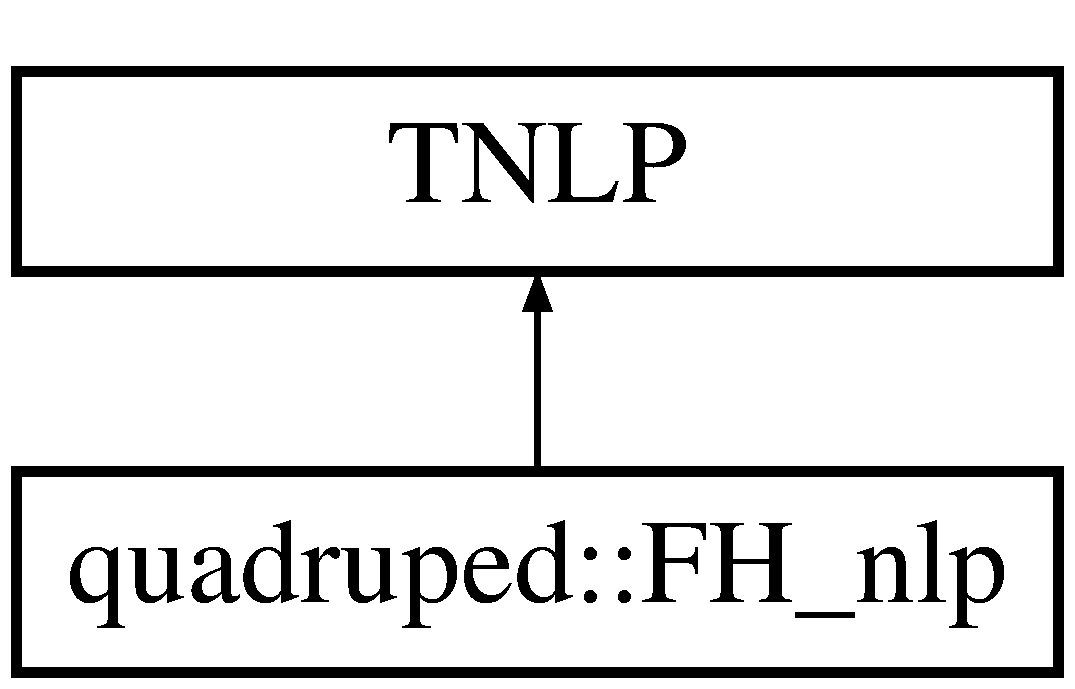
\includegraphics[height=2.000000cm]{classquadruped_1_1FH__nlp}
\end{center}
\end{figure}
\subsection*{Public 成员函数}
\begin{DoxyCompactItemize}
\item 
\hyperlink{classquadruped_1_1FH__nlp_a2681be275f98fa7ca224ac7d03cf822e}{F\+H\+\_\+nlp} (\hyperlink{classquadruped_1_1FH__updataInfo}{F\+H\+\_\+updata\+Info} $\ast$p\+\_\+updata\+Info)
\item 
virtual bool \hyperlink{classquadruped_1_1FH__nlp_a2a7f67c823cce5ba75b8ba14a4beccfa}{get\+\_\+nlp\+\_\+info} (Index \&n, Index \&m, Index \&nnz\+\_\+jac\+\_\+g, Index \&nnz\+\_\+h\+\_\+lag, Index\+Style\+Enum \&index\+\_\+style)
\item 
virtual bool \hyperlink{classquadruped_1_1FH__nlp_a8f2ccc29742196f79b90ffd597b63927}{get\+\_\+bounds\+\_\+info} (Index n, Number $\ast$x\+\_\+l, Number $\ast$x\+\_\+u, Index m, Number $\ast$g\+\_\+l, Number $\ast$g\+\_\+u)
\item 
virtual bool \hyperlink{classquadruped_1_1FH__nlp_a97e90c5109ca64c20b27f767d5665df4}{get\+\_\+starting\+\_\+point} (Index n, bool init\+\_\+x, Number $\ast$x, bool init\+\_\+z, Number $\ast$z\+\_\+L, Number $\ast$z\+\_\+U, Index m, bool init\+\_\+lambda, Number $\ast$lambda)
\item 
virtual bool \hyperlink{classquadruped_1_1FH__nlp_a1c50f2e5601d9cfadf569d7dae7ba787}{eval\+\_\+f} (Index n, const Number $\ast$x, bool new\+\_\+x, Number \&obj\+\_\+value)
\item 
virtual bool \hyperlink{classquadruped_1_1FH__nlp_aace436330eee6fd6e4e86ec2221a8a35}{eval\+\_\+grad\+\_\+f} (Index n, const Number $\ast$x, bool new\+\_\+x, Number $\ast$grad\+\_\+f)
\item 
virtual bool \hyperlink{classquadruped_1_1FH__nlp_a6451ea1ebe787cc94fe34199193c7acd}{eval\+\_\+g} (Index n, const Number $\ast$x, bool new\+\_\+x, Index m, Number $\ast$g)
\item 
virtual bool \hyperlink{classquadruped_1_1FH__nlp_adc432f17a942b28d5cd9ac261361692d}{eval\+\_\+jac\+\_\+g} (Index n, const Number $\ast$x, bool new\+\_\+x, Index m, Index nele\+\_\+jac, Index $\ast$i\+Row, Index $\ast$j\+Col, Number $\ast$values)
\item 
virtual bool \hyperlink{classquadruped_1_1FH__nlp_a19a232662e043d038b3184ccac74e679}{eval\+\_\+h} (Index n, const Number $\ast$x, bool new\+\_\+x, Number obj\+\_\+factor, Index m, const Number $\ast$lambda, bool new\+\_\+lambda, Index nele\+\_\+hess, Index $\ast$i\+Row, Index $\ast$j\+Col, Number $\ast$values)
\end{DoxyCompactItemize}
\begin{Indent}\textbf{ Solution Methods}\par
\begin{DoxyCompactItemize}
\item 
virtual void \hyperlink{classquadruped_1_1FH__nlp_aae99a7bb4a2e1eb7fee96440583fae95}{finalize\+\_\+solution} (Solver\+Return status, Index n, const Number $\ast$x, const Number $\ast$z\+\_\+L, const Number $\ast$z\+\_\+U, Index m, const Number $\ast$g, const Number $\ast$lambda, Number obj\+\_\+value, const Ipopt\+Data $\ast$ip\+\_\+data, Ipopt\+Calculated\+Quantities $\ast$ip\+\_\+cq)
\end{DoxyCompactItemize}
\end{Indent}
\subsection*{Public 属性}
\begin{DoxyCompactItemize}
\item 
\mbox{\Hypertarget{classquadruped_1_1FH__nlp_a4344579b63950206ce985d234a3266fd}\label{classquadruped_1_1FH__nlp_a4344579b63950206ce985d234a3266fd}} 
int {\bfseries var\+\_\+num}
\item 
\mbox{\Hypertarget{classquadruped_1_1FH__nlp_abb85add767802a38175db2a34323cae3}\label{classquadruped_1_1FH__nlp_abb85add767802a38175db2a34323cae3}} 
int {\bfseries cst\+\_\+num}
\item 
\mbox{\Hypertarget{classquadruped_1_1FH__nlp_a975ab9034fd3d5cb9c22d7afbd6929cf}\label{classquadruped_1_1FH__nlp_a975ab9034fd3d5cb9c22d7afbd6929cf}} 
int {\bfseries cst\+\_\+jac\+\_\+num}
\item 
\mbox{\Hypertarget{classquadruped_1_1FH__nlp_a9a73d743c633605649b0664ab7a8a488}\label{classquadruped_1_1FH__nlp_a9a73d743c633605649b0664ab7a8a488}} 
int {\bfseries cst\+\_\+hes\+\_\+num}
\end{DoxyCompactItemize}


\subsection{构造及析构函数说明}
\mbox{\Hypertarget{classquadruped_1_1FH__nlp_a2681be275f98fa7ca224ac7d03cf822e}\label{classquadruped_1_1FH__nlp_a2681be275f98fa7ca224ac7d03cf822e}} 
\index{quadruped\+::\+F\+H\+\_\+nlp@{quadruped\+::\+F\+H\+\_\+nlp}!F\+H\+\_\+nlp@{F\+H\+\_\+nlp}}
\index{F\+H\+\_\+nlp@{F\+H\+\_\+nlp}!quadruped\+::\+F\+H\+\_\+nlp@{quadruped\+::\+F\+H\+\_\+nlp}}
\subsubsection{\texorpdfstring{F\+H\+\_\+nlp()}{FH\_nlp()}}
{\footnotesize\ttfamily F\+H\+\_\+nlp\+::\+F\+H\+\_\+nlp (\begin{DoxyParamCaption}\item[{\hyperlink{classquadruped_1_1FH__updataInfo}{F\+H\+\_\+updata\+Info} $\ast$}]{p\+\_\+updata\+Info }\end{DoxyParamCaption})\hspace{0.3cm}{\ttfamily [explicit]}}

\+: 非线性规划问题参数设置 
\begin{DoxyParams}{参数}
{\em \{\+F\+H\+\_\+updata\+Info$\ast$\}} & p\+\_\+updata\+Info 落足点规划的信息更新对象 \\
\hline
\end{DoxyParams}
\begin{DoxyReturn}{返回}
\{$\ast$\} 
\end{DoxyReturn}


参考 F\+H\+\_\+\+V\+A\+R\+\_\+\+N\+U\+M\+\_\+\+S\+I\+N\+G\+LE.



\subsection{成员函数说明}
\mbox{\Hypertarget{classquadruped_1_1FH__nlp_a1c50f2e5601d9cfadf569d7dae7ba787}\label{classquadruped_1_1FH__nlp_a1c50f2e5601d9cfadf569d7dae7ba787}} 
\index{quadruped\+::\+F\+H\+\_\+nlp@{quadruped\+::\+F\+H\+\_\+nlp}!eval\+\_\+f@{eval\+\_\+f}}
\index{eval\+\_\+f@{eval\+\_\+f}!quadruped\+::\+F\+H\+\_\+nlp@{quadruped\+::\+F\+H\+\_\+nlp}}
\subsubsection{\texorpdfstring{eval\+\_\+f()}{eval\_f()}}
{\footnotesize\ttfamily bool F\+H\+\_\+nlp\+::eval\+\_\+f (\begin{DoxyParamCaption}\item[{Index}]{n,  }\item[{const Number $\ast$}]{x,  }\item[{bool}]{new\+\_\+x,  }\item[{Number \&}]{obj\+\_\+value }\end{DoxyParamCaption})\hspace{0.3cm}{\ttfamily [virtual]}}

Method to return the objective value

\+: 目标函数，这里为常数0 
\begin{DoxyParams}{参数}
{\em \{$\ast$\}} & \\
\hline
\end{DoxyParams}
\begin{DoxyReturn}{返回}
\{$\ast$\} 
\end{DoxyReturn}
\mbox{\Hypertarget{classquadruped_1_1FH__nlp_a6451ea1ebe787cc94fe34199193c7acd}\label{classquadruped_1_1FH__nlp_a6451ea1ebe787cc94fe34199193c7acd}} 
\index{quadruped\+::\+F\+H\+\_\+nlp@{quadruped\+::\+F\+H\+\_\+nlp}!eval\+\_\+g@{eval\+\_\+g}}
\index{eval\+\_\+g@{eval\+\_\+g}!quadruped\+::\+F\+H\+\_\+nlp@{quadruped\+::\+F\+H\+\_\+nlp}}
\subsubsection{\texorpdfstring{eval\+\_\+g()}{eval\_g()}}
{\footnotesize\ttfamily bool F\+H\+\_\+nlp\+::eval\+\_\+g (\begin{DoxyParamCaption}\item[{Index}]{n,  }\item[{const Number $\ast$}]{x,  }\item[{bool}]{new\+\_\+x,  }\item[{Index}]{m,  }\item[{Number $\ast$}]{g }\end{DoxyParamCaption})\hspace{0.3cm}{\ttfamily [virtual]}}

Method to return the constraint residuals

\+: 计算约束的值 
\begin{DoxyParams}{参数}
{\em \{\+Index\}} & n \\
\hline
{\em \{const} & Number$\ast$\} x \\
\hline
{\em \{bool\}} & new\+\_\+x \\
\hline
{\em \{\+Index\}} & m \\
\hline
{\em \{\+Number$\ast$\}} & g \\
\hline
\end{DoxyParams}
\begin{DoxyReturn}{返回}
\{$\ast$\} 
\end{DoxyReturn}


参考 quadruped\+::\+F\+H\+\_\+constraints\+::\+Get\+Kinematics\+Cst() , 以及 quadruped\+::\+F\+H\+\_\+constraints\+::\+Get\+Other\+Cst().

\mbox{\Hypertarget{classquadruped_1_1FH__nlp_aace436330eee6fd6e4e86ec2221a8a35}\label{classquadruped_1_1FH__nlp_aace436330eee6fd6e4e86ec2221a8a35}} 
\index{quadruped\+::\+F\+H\+\_\+nlp@{quadruped\+::\+F\+H\+\_\+nlp}!eval\+\_\+grad\+\_\+f@{eval\+\_\+grad\+\_\+f}}
\index{eval\+\_\+grad\+\_\+f@{eval\+\_\+grad\+\_\+f}!quadruped\+::\+F\+H\+\_\+nlp@{quadruped\+::\+F\+H\+\_\+nlp}}
\subsubsection{\texorpdfstring{eval\+\_\+grad\+\_\+f()}{eval\_grad\_f()}}
{\footnotesize\ttfamily bool F\+H\+\_\+nlp\+::eval\+\_\+grad\+\_\+f (\begin{DoxyParamCaption}\item[{Index}]{n,  }\item[{const Number $\ast$}]{x,  }\item[{bool}]{new\+\_\+x,  }\item[{Number $\ast$}]{grad\+\_\+f }\end{DoxyParamCaption})\hspace{0.3cm}{\ttfamily [virtual]}}

Method to return the gradient of the objective

\+: 目标函数的梯度 
\begin{DoxyParams}{参数}
{\em \{$\ast$\}} & \\
\hline
\end{DoxyParams}
\begin{DoxyReturn}{返回}
\{$\ast$\} 
\end{DoxyReturn}
\mbox{\Hypertarget{classquadruped_1_1FH__nlp_a19a232662e043d038b3184ccac74e679}\label{classquadruped_1_1FH__nlp_a19a232662e043d038b3184ccac74e679}} 
\index{quadruped\+::\+F\+H\+\_\+nlp@{quadruped\+::\+F\+H\+\_\+nlp}!eval\+\_\+h@{eval\+\_\+h}}
\index{eval\+\_\+h@{eval\+\_\+h}!quadruped\+::\+F\+H\+\_\+nlp@{quadruped\+::\+F\+H\+\_\+nlp}}
\subsubsection{\texorpdfstring{eval\+\_\+h()}{eval\_h()}}
{\footnotesize\ttfamily bool F\+H\+\_\+nlp\+::eval\+\_\+h (\begin{DoxyParamCaption}\item[{Index}]{n,  }\item[{const Number $\ast$}]{x,  }\item[{bool}]{new\+\_\+x,  }\item[{Number}]{obj\+\_\+factor,  }\item[{Index}]{m,  }\item[{const Number $\ast$}]{lambda,  }\item[{bool}]{new\+\_\+lambda,  }\item[{Index}]{nele\+\_\+hess,  }\item[{Index $\ast$}]{i\+Row,  }\item[{Index $\ast$}]{j\+Col,  }\item[{Number $\ast$}]{values }\end{DoxyParamCaption})\hspace{0.3cm}{\ttfamily [virtual]}}

Method to return\+: 1) The structure of the hessian of the lagrangian (if \char`\"{}values\char`\"{} is N\+U\+LL) 2) The values of the hessian of the lagrangian (if \char`\"{}values\char`\"{} is not N\+U\+LL)

\+: 目标函数和约束的海森矩阵 
\begin{DoxyParams}{参数}
{\em \{$\ast$\}} & \\
\hline
\end{DoxyParams}
\begin{DoxyReturn}{返回}
\{$\ast$\} 
\end{DoxyReturn}


参考 F\+H\+\_\+\+V\+A\+R\+\_\+\+N\+U\+M\+\_\+\+S\+I\+N\+G\+LE.

\mbox{\Hypertarget{classquadruped_1_1FH__nlp_adc432f17a942b28d5cd9ac261361692d}\label{classquadruped_1_1FH__nlp_adc432f17a942b28d5cd9ac261361692d}} 
\index{quadruped\+::\+F\+H\+\_\+nlp@{quadruped\+::\+F\+H\+\_\+nlp}!eval\+\_\+jac\+\_\+g@{eval\+\_\+jac\+\_\+g}}
\index{eval\+\_\+jac\+\_\+g@{eval\+\_\+jac\+\_\+g}!quadruped\+::\+F\+H\+\_\+nlp@{quadruped\+::\+F\+H\+\_\+nlp}}
\subsubsection{\texorpdfstring{eval\+\_\+jac\+\_\+g()}{eval\_jac\_g()}}
{\footnotesize\ttfamily bool F\+H\+\_\+nlp\+::eval\+\_\+jac\+\_\+g (\begin{DoxyParamCaption}\item[{Index}]{n,  }\item[{const Number $\ast$}]{x,  }\item[{bool}]{new\+\_\+x,  }\item[{Index}]{m,  }\item[{Index}]{nele\+\_\+jac,  }\item[{Index $\ast$}]{i\+Row,  }\item[{Index $\ast$}]{j\+Col,  }\item[{Number $\ast$}]{values }\end{DoxyParamCaption})\hspace{0.3cm}{\ttfamily [virtual]}}

Method to return\+: 1) The structure of the jacobian (if \char`\"{}values\char`\"{} is N\+U\+LL) 2) The values of the jacobian (if \char`\"{}values\char`\"{} is not N\+U\+LL)

\+: 约束的雅可比矩阵 
\begin{DoxyParams}{参数}
{\em \{$\ast$\}} & \\
\hline
\end{DoxyParams}
\begin{DoxyReturn}{返回}
\{$\ast$\} 
\end{DoxyReturn}
\mbox{\Hypertarget{classquadruped_1_1FH__nlp_aae99a7bb4a2e1eb7fee96440583fae95}\label{classquadruped_1_1FH__nlp_aae99a7bb4a2e1eb7fee96440583fae95}} 
\index{quadruped\+::\+F\+H\+\_\+nlp@{quadruped\+::\+F\+H\+\_\+nlp}!finalize\+\_\+solution@{finalize\+\_\+solution}}
\index{finalize\+\_\+solution@{finalize\+\_\+solution}!quadruped\+::\+F\+H\+\_\+nlp@{quadruped\+::\+F\+H\+\_\+nlp}}
\subsubsection{\texorpdfstring{finalize\+\_\+solution()}{finalize\_solution()}}
{\footnotesize\ttfamily void F\+H\+\_\+nlp\+::finalize\+\_\+solution (\begin{DoxyParamCaption}\item[{Solver\+Return}]{status,  }\item[{Index}]{n,  }\item[{const Number $\ast$}]{x,  }\item[{const Number $\ast$}]{z\+\_\+L,  }\item[{const Number $\ast$}]{z\+\_\+U,  }\item[{Index}]{m,  }\item[{const Number $\ast$}]{g,  }\item[{const Number $\ast$}]{lambda,  }\item[{Number}]{obj\+\_\+value,  }\item[{const Ipopt\+Data $\ast$}]{ip\+\_\+data,  }\item[{Ipopt\+Calculated\+Quantities $\ast$}]{ip\+\_\+cq }\end{DoxyParamCaption})\hspace{0.3cm}{\ttfamily [virtual]}}

This method is called when the algorithm is complete so the T\+N\+LP can store/write the solution

\+: 优化结果 
\begin{DoxyParams}{参数}
{\em \{$\ast$\}} & \\
\hline
\end{DoxyParams}
\begin{DoxyReturn}{返回}
\{$\ast$\} 
\end{DoxyReturn}
\mbox{\Hypertarget{classquadruped_1_1FH__nlp_a8f2ccc29742196f79b90ffd597b63927}\label{classquadruped_1_1FH__nlp_a8f2ccc29742196f79b90ffd597b63927}} 
\index{quadruped\+::\+F\+H\+\_\+nlp@{quadruped\+::\+F\+H\+\_\+nlp}!get\+\_\+bounds\+\_\+info@{get\+\_\+bounds\+\_\+info}}
\index{get\+\_\+bounds\+\_\+info@{get\+\_\+bounds\+\_\+info}!quadruped\+::\+F\+H\+\_\+nlp@{quadruped\+::\+F\+H\+\_\+nlp}}
\subsubsection{\texorpdfstring{get\+\_\+bounds\+\_\+info()}{get\_bounds\_info()}}
{\footnotesize\ttfamily bool F\+H\+\_\+nlp\+::get\+\_\+bounds\+\_\+info (\begin{DoxyParamCaption}\item[{Index}]{n,  }\item[{Number $\ast$}]{x\+\_\+l,  }\item[{Number $\ast$}]{x\+\_\+u,  }\item[{Index}]{m,  }\item[{Number $\ast$}]{g\+\_\+l,  }\item[{Number $\ast$}]{g\+\_\+u }\end{DoxyParamCaption})\hspace{0.3cm}{\ttfamily [virtual]}}

Method to return the bounds for my problem

\+: 设置边界 
\begin{DoxyParams}{参数}
{\em \{$\ast$\}} & \\
\hline
\end{DoxyParams}
\begin{DoxyReturn}{返回}
\{$\ast$\} 
\end{DoxyReturn}


参考 F\+H\+\_\+\+V\+A\+R\+\_\+\+N\+U\+M\+\_\+\+S\+I\+N\+G\+LE , 以及 quadruped\+::\+F\+H\+\_\+updata\+Info\+::\+Get\+X\+Bound().

\mbox{\Hypertarget{classquadruped_1_1FH__nlp_a2a7f67c823cce5ba75b8ba14a4beccfa}\label{classquadruped_1_1FH__nlp_a2a7f67c823cce5ba75b8ba14a4beccfa}} 
\index{quadruped\+::\+F\+H\+\_\+nlp@{quadruped\+::\+F\+H\+\_\+nlp}!get\+\_\+nlp\+\_\+info@{get\+\_\+nlp\+\_\+info}}
\index{get\+\_\+nlp\+\_\+info@{get\+\_\+nlp\+\_\+info}!quadruped\+::\+F\+H\+\_\+nlp@{quadruped\+::\+F\+H\+\_\+nlp}}
\subsubsection{\texorpdfstring{get\+\_\+nlp\+\_\+info()}{get\_nlp\_info()}}
{\footnotesize\ttfamily bool F\+H\+\_\+nlp\+::get\+\_\+nlp\+\_\+info (\begin{DoxyParamCaption}\item[{Index \&}]{n,  }\item[{Index \&}]{m,  }\item[{Index \&}]{nnz\+\_\+jac\+\_\+g,  }\item[{Index \&}]{nnz\+\_\+h\+\_\+lag,  }\item[{Index\+Style\+Enum \&}]{index\+\_\+style }\end{DoxyParamCaption})\hspace{0.3cm}{\ttfamily [virtual]}}

ipopt function Method to return some info about the nlp

\+: 非线性规划问题参数设置 
\begin{DoxyParams}{参数}
{\em \{\+F\+H\+\_\+updata\+Info$\ast$\}} & p\+\_\+updata\+Info \\
\hline
\end{DoxyParams}
\begin{DoxyReturn}{返回}
\{$\ast$\} 
\end{DoxyReturn}
\mbox{\Hypertarget{classquadruped_1_1FH__nlp_a97e90c5109ca64c20b27f767d5665df4}\label{classquadruped_1_1FH__nlp_a97e90c5109ca64c20b27f767d5665df4}} 
\index{quadruped\+::\+F\+H\+\_\+nlp@{quadruped\+::\+F\+H\+\_\+nlp}!get\+\_\+starting\+\_\+point@{get\+\_\+starting\+\_\+point}}
\index{get\+\_\+starting\+\_\+point@{get\+\_\+starting\+\_\+point}!quadruped\+::\+F\+H\+\_\+nlp@{quadruped\+::\+F\+H\+\_\+nlp}}
\subsubsection{\texorpdfstring{get\+\_\+starting\+\_\+point()}{get\_starting\_point()}}
{\footnotesize\ttfamily bool F\+H\+\_\+nlp\+::get\+\_\+starting\+\_\+point (\begin{DoxyParamCaption}\item[{Index}]{n,  }\item[{bool}]{init\+\_\+x,  }\item[{Number $\ast$}]{x,  }\item[{bool}]{init\+\_\+z,  }\item[{Number $\ast$}]{z\+\_\+L,  }\item[{Number $\ast$}]{z\+\_\+U,  }\item[{Index}]{m,  }\item[{bool}]{init\+\_\+lambda,  }\item[{Number $\ast$}]{lambda }\end{DoxyParamCaption})\hspace{0.3cm}{\ttfamily [virtual]}}

Method to return the starting point for the algorithm

\+: 配置初始点 
\begin{DoxyParams}{参数}
{\em \{$\ast$\}} & \\
\hline
\end{DoxyParams}
\begin{DoxyReturn}{返回}
\{$\ast$\} 
\end{DoxyReturn}


参考 quadruped\+::\+F\+H\+\_\+updata\+Info\+::\+Get\+X\+Inital().



该类的文档由以下文件生成\+:\begin{DoxyCompactItemize}
\item 
controller/motion\+Plan/foothold/f\+H\+\_\+nlp.\+hpp\item 
controller/motion\+Plan/foothold/\hyperlink{fH__nlp_8cpp}{f\+H\+\_\+nlp.\+cpp}\end{DoxyCompactItemize}

\hypertarget{classquadruped_1_1FH__updataInfo}{}\section{quadruped\+:\+:F\+H\+\_\+updata\+Info类 参考}
\label{classquadruped_1_1FH__updataInfo}\index{quadruped\+::\+F\+H\+\_\+updata\+Info@{quadruped\+::\+F\+H\+\_\+updata\+Info}}


Actiger落足点规划信息更新类  




{\ttfamily \#include $<$f\+H\+\_\+updata\+Info.\+hpp$>$}

\subsection*{Public 成员函数}
\begin{DoxyCompactItemize}
\item 
\mbox{\Hypertarget{classquadruped_1_1FH__updataInfo_a02285dcf0fbee8e7fe0b632648b9e8e9}\label{classquadruped_1_1FH__updataInfo_a02285dcf0fbee8e7fe0b632648b9e8e9}} 
{\bfseries F\+H\+\_\+updata\+Info} (\hyperlink{classquadruped_1_1Parameters}{Parameters} $\ast$p\+\_\+para, \hyperlink{classquadruped_1_1Terrain}{Terrain} $\ast$p\+\_\+terrain\+\_\+now)
\item 
void \hyperlink{classquadruped_1_1FH__updataInfo_a1ef2f860fc18a7176f6b9ffc694778ee}{Get\+X\+Bound} (double $\ast$ub, double $\ast$lb)
\item 
\mbox{\Hypertarget{classquadruped_1_1FH__updataInfo_a8c3842af225ae629a1db0fe201c3cabc}\label{classquadruped_1_1FH__updataInfo_a8c3842af225ae629a1db0fe201c3cabc}} 
void {\bfseries Set\+Terrain} (uint8\+\_\+t p\+\_\+terrain\+Type)
\item 
void \hyperlink{classquadruped_1_1FH__updataInfo_a75b04f959df3aee0f49e0c8627754792}{Get\+X\+Inital} (double $\ast$x)
\item 
void \hyperlink{classquadruped_1_1FH__updataInfo_a4f87f044f37ed293b1e86802cf41345f}{Update\+Info} (int p\+\_\+is\+\_\+lf\+\_\+rr\+\_\+stand, \hyperlink{cppTypes_8h_a65c27bf97693676535dd0b30ea0ad399}{Vec3}$<$ double $>$ p\+\_\+cur\+Euler, \hyperlink{cppTypes_8h_a65c27bf97693676535dd0b30ea0ad399}{Vec3}$<$ double $>$ p\+\_\+cur\+Pos, \hyperlink{cppTypes_8h_a65c27bf97693676535dd0b30ea0ad399}{Vec3}$<$ double $>$ p\+\_\+cur\+Velocity, double p\+\_\+desire\+\_\+yaw, double p\+\_\+desire\+\_\+z, \hyperlink{cppTypes_8h_a65c27bf97693676535dd0b30ea0ad399}{Vec3}$<$ double $>$ p\+\_\+endfoot\+\_\+now\+\_\+front, \hyperlink{cppTypes_8h_a65c27bf97693676535dd0b30ea0ad399}{Vec3}$<$ double $>$ p\+\_\+endfoot\+\_\+now\+\_\+rear, \hyperlink{cppTypes_8h_a65c27bf97693676535dd0b30ea0ad399}{Vec3}$<$ double $>$ p\+\_\+stance\+\_\+now\+\_\+front, \hyperlink{cppTypes_8h_a65c27bf97693676535dd0b30ea0ad399}{Vec3}$<$ double $>$ p\+\_\+stance\+\_\+now\+\_\+rear)
\end{DoxyCompactItemize}
\subsection*{Public 属性}
\begin{DoxyCompactItemize}
\item 
\mbox{\Hypertarget{classquadruped_1_1FH__updataInfo_a49f9573bc207819187f35080fc098c9e}\label{classquadruped_1_1FH__updataInfo_a49f9573bc207819187f35080fc098c9e}} 
bool \hyperlink{classquadruped_1_1FH__updataInfo_a49f9573bc207819187f35080fc098c9e}{is\+\_\+lf\+\_\+rr\+\_\+stand}
\begin{DoxyCompactList}\small\item\em 当前的支撑腿组合标志位 \end{DoxyCompactList}\item 
\mbox{\Hypertarget{classquadruped_1_1FH__updataInfo_af22df9a440b401aceb06055054ef385e}\label{classquadruped_1_1FH__updataInfo_af22df9a440b401aceb06055054ef385e}} 
double \hyperlink{classquadruped_1_1FH__updataInfo_af22df9a440b401aceb06055054ef385e}{desire\+\_\+z}
\begin{DoxyCompactList}\small\item\em Actiger期望的机体高度 \end{DoxyCompactList}\item 
\mbox{\Hypertarget{classquadruped_1_1FH__updataInfo_ac34eaa41e1f6cb0e3ddbc6ffa608e157}\label{classquadruped_1_1FH__updataInfo_ac34eaa41e1f6cb0e3ddbc6ffa608e157}} 
double \hyperlink{classquadruped_1_1FH__updataInfo_ac34eaa41e1f6cb0e3ddbc6ffa608e157}{desire\+\_\+yaw}
\begin{DoxyCompactList}\small\item\em Actiger期望的机体高度 \end{DoxyCompactList}\item 
\mbox{\Hypertarget{classquadruped_1_1FH__updataInfo_ab1c5aaff85dc956883ae6336f327d49f}\label{classquadruped_1_1FH__updataInfo_ab1c5aaff85dc956883ae6336f327d49f}} 
double {\bfseries desire\+\_\+hight}
\item 
\mbox{\Hypertarget{classquadruped_1_1FH__updataInfo_a70ab4c64d1af0bd7bddcc37378324380}\label{classquadruped_1_1FH__updataInfo_a70ab4c64d1af0bd7bddcc37378324380}} 
double {\bfseries des\+Endfoot\+\_\+pos\+\_\+z\+\_\+front}
\item 
\mbox{\Hypertarget{classquadruped_1_1FH__updataInfo_acaf9672ba88be96c5871b1e366b73542}\label{classquadruped_1_1FH__updataInfo_acaf9672ba88be96c5871b1e366b73542}} 
double {\bfseries des\+Endfoot\+\_\+pos\+\_\+z\+\_\+rear}
\item 
\mbox{\Hypertarget{classquadruped_1_1FH__updataInfo_a33689880d3dda1f5a5021913433abf6d}\label{classquadruped_1_1FH__updataInfo_a33689880d3dda1f5a5021913433abf6d}} 
\hyperlink{cppTypes_8h_a65c27bf97693676535dd0b30ea0ad399}{Vec3}$<$ double $>$ {\bfseries cmd\+Velocity}
\item 
\mbox{\Hypertarget{classquadruped_1_1FH__updataInfo_a1e400165216fd290b6b792a5c88797b8}\label{classquadruped_1_1FH__updataInfo_a1e400165216fd290b6b792a5c88797b8}} 
\hyperlink{cppTypes_8h_a65c27bf97693676535dd0b30ea0ad399}{Vec3}$<$ double $>$ {\bfseries des\+Velocity}
\item 
\mbox{\Hypertarget{classquadruped_1_1FH__updataInfo_aed247377d5ad5f622ea2a8b1163f8b9d}\label{classquadruped_1_1FH__updataInfo_aed247377d5ad5f622ea2a8b1163f8b9d}} 
\hyperlink{cppTypes_8h_a65c27bf97693676535dd0b30ea0ad399}{Vec3}$<$ double $>$ {\bfseries des\+Omega}
\item 
\mbox{\Hypertarget{classquadruped_1_1FH__updataInfo_aa67e71cdea575a57b111904071d2d10b}\label{classquadruped_1_1FH__updataInfo_aa67e71cdea575a57b111904071d2d10b}} 
\hyperlink{cppTypes_8h_a65c27bf97693676535dd0b30ea0ad399}{Vec3}$<$ double $>$ {\bfseries des\+Euler}
\item 
\mbox{\Hypertarget{classquadruped_1_1FH__updataInfo_a0f4eac9bb4220364bcbf16d9cc41f48f}\label{classquadruped_1_1FH__updataInfo_a0f4eac9bb4220364bcbf16d9cc41f48f}} 
\hyperlink{cppTypes_8h_a65c27bf97693676535dd0b30ea0ad399}{Vec3}$<$ double $>$ {\bfseries cur\+Pos}
\item 
\mbox{\Hypertarget{classquadruped_1_1FH__updataInfo_a0e6b7472adec0a3be775bfdb83d90258}\label{classquadruped_1_1FH__updataInfo_a0e6b7472adec0a3be775bfdb83d90258}} 
\hyperlink{cppTypes_8h_a65c27bf97693676535dd0b30ea0ad399}{Vec3}$<$ double $>$ {\bfseries cur\+Euler}
\item 
\mbox{\Hypertarget{classquadruped_1_1FH__updataInfo_a80b0a81421e7a1c29f5494a77f5fc2b3}\label{classquadruped_1_1FH__updataInfo_a80b0a81421e7a1c29f5494a77f5fc2b3}} 
\hyperlink{cppTypes_8h_a65c27bf97693676535dd0b30ea0ad399}{Vec3}$<$ double $>$ {\bfseries cur\+Velocity}
\item 
\mbox{\Hypertarget{classquadruped_1_1FH__updataInfo_a6c28594f6924b51c70c5a320e464fb79}\label{classquadruped_1_1FH__updataInfo_a6c28594f6924b51c70c5a320e464fb79}} 
\hyperlink{cppTypes_8h_a65c27bf97693676535dd0b30ea0ad399}{Vec3}$<$ double $>$ {\bfseries body\+Pos\+\_\+desire}
\item 
\mbox{\Hypertarget{classquadruped_1_1FH__updataInfo_a3fb2708c9e8ee09efbb40354e692bfee}\label{classquadruped_1_1FH__updataInfo_a3fb2708c9e8ee09efbb40354e692bfee}} 
\hyperlink{cppTypes_8h_a65c27bf97693676535dd0b30ea0ad399}{Vec3}$<$ double $>$ {\bfseries endfoot\+\_\+now\+\_\+front}
\item 
\mbox{\Hypertarget{classquadruped_1_1FH__updataInfo_a25bb037f942e458bde9f53095a7bbcae}\label{classquadruped_1_1FH__updataInfo_a25bb037f942e458bde9f53095a7bbcae}} 
\hyperlink{cppTypes_8h_a65c27bf97693676535dd0b30ea0ad399}{Vec3}$<$ double $>$ {\bfseries endfoot\+\_\+desire\+\_\+front}
\item 
\mbox{\Hypertarget{classquadruped_1_1FH__updataInfo_a0d706c45d632aee4e7412afb64b60abc}\label{classquadruped_1_1FH__updataInfo_a0d706c45d632aee4e7412afb64b60abc}} 
\hyperlink{cppTypes_8h_a685282630cf228cbde6112c5e6f713c3}{Vec2}$<$ double $>$ {\bfseries foothold\+\_\+front\+\_\+min}
\item 
\mbox{\Hypertarget{classquadruped_1_1FH__updataInfo_a58c5797c7bce7f4ed51b56aa877eabcc}\label{classquadruped_1_1FH__updataInfo_a58c5797c7bce7f4ed51b56aa877eabcc}} 
\hyperlink{cppTypes_8h_a685282630cf228cbde6112c5e6f713c3}{Vec2}$<$ double $>$ {\bfseries foothold\+\_\+front\+\_\+max}
\item 
\mbox{\Hypertarget{classquadruped_1_1FH__updataInfo_a1ccae3e3285ccc9aa9b09b03a3b65fb0}\label{classquadruped_1_1FH__updataInfo_a1ccae3e3285ccc9aa9b09b03a3b65fb0}} 
\hyperlink{cppTypes_8h_a65c27bf97693676535dd0b30ea0ad399}{Vec3}$<$ double $>$ {\bfseries endfoot\+\_\+now\+\_\+rear}
\item 
\mbox{\Hypertarget{classquadruped_1_1FH__updataInfo_a8f2b0ee92524c5402f04f7004b04c61e}\label{classquadruped_1_1FH__updataInfo_a8f2b0ee92524c5402f04f7004b04c61e}} 
\hyperlink{cppTypes_8h_a65c27bf97693676535dd0b30ea0ad399}{Vec3}$<$ double $>$ {\bfseries endfoot\+\_\+desire\+\_\+rear}
\item 
\mbox{\Hypertarget{classquadruped_1_1FH__updataInfo_a9edff2ef2b865628d69543965b79664b}\label{classquadruped_1_1FH__updataInfo_a9edff2ef2b865628d69543965b79664b}} 
\hyperlink{cppTypes_8h_a685282630cf228cbde6112c5e6f713c3}{Vec2}$<$ double $>$ {\bfseries foothold\+\_\+rear\+\_\+min}
\item 
\mbox{\Hypertarget{classquadruped_1_1FH__updataInfo_a3e0ad49ac6f0a41100a0be93443e278b}\label{classquadruped_1_1FH__updataInfo_a3e0ad49ac6f0a41100a0be93443e278b}} 
\hyperlink{cppTypes_8h_a685282630cf228cbde6112c5e6f713c3}{Vec2}$<$ double $>$ {\bfseries foothold\+\_\+rear\+\_\+max}
\item 
\mbox{\Hypertarget{classquadruped_1_1FH__updataInfo_ae55cf1ca302eebfab28171fd9945552f}\label{classquadruped_1_1FH__updataInfo_ae55cf1ca302eebfab28171fd9945552f}} 
\hyperlink{cppTypes_8h_a65c27bf97693676535dd0b30ea0ad399}{Vec3}$<$ double $>$ {\bfseries stance\+\_\+front\+\_\+pos}
\item 
\mbox{\Hypertarget{classquadruped_1_1FH__updataInfo_ae5c5f31d3eabd61ff2cccd0ccba4b501}\label{classquadruped_1_1FH__updataInfo_ae5c5f31d3eabd61ff2cccd0ccba4b501}} 
\hyperlink{cppTypes_8h_a65c27bf97693676535dd0b30ea0ad399}{Vec3}$<$ double $>$ {\bfseries stance\+\_\+rear\+\_\+pos}
\item 
\mbox{\Hypertarget{classquadruped_1_1FH__updataInfo_a58bd8b51eb75ed84de0e676dc9d22086}\label{classquadruped_1_1FH__updataInfo_a58bd8b51eb75ed84de0e676dc9d22086}} 
\hyperlink{cppTypes_8h_a685282630cf228cbde6112c5e6f713c3}{Vec2}$<$ double $>$ {\bfseries hip\+\_\+2\+\_\+body\+\_\+front}
\item 
\mbox{\Hypertarget{classquadruped_1_1FH__updataInfo_a7341323288bfd1bf94f57c9edf5db1b7}\label{classquadruped_1_1FH__updataInfo_a7341323288bfd1bf94f57c9edf5db1b7}} 
\hyperlink{cppTypes_8h_a685282630cf228cbde6112c5e6f713c3}{Vec2}$<$ double $>$ {\bfseries hip\+\_\+2\+\_\+body\+\_\+rear}
\item 
\mbox{\Hypertarget{classquadruped_1_1FH__updataInfo_a36affd5f8b07dfa83241aa5760d070c4}\label{classquadruped_1_1FH__updataInfo_a36affd5f8b07dfa83241aa5760d070c4}} 
double {\bfseries body\+\_\+length}
\item 
\mbox{\Hypertarget{classquadruped_1_1FH__updataInfo_a53630e42511df6e5f3348ea3d3a71fa1}\label{classquadruped_1_1FH__updataInfo_a53630e42511df6e5f3348ea3d3a71fa1}} 
double {\bfseries body\+\_\+width}
\item 
\mbox{\Hypertarget{classquadruped_1_1FH__updataInfo_ab2d716cfa3e309ab263228c2a559d1b3}\label{classquadruped_1_1FH__updataInfo_ab2d716cfa3e309ab263228c2a559d1b3}} 
double {\bfseries Ts}
\item 
\mbox{\Hypertarget{classquadruped_1_1FH__updataInfo_aeba358aad0639518539d26c067c23d43}\label{classquadruped_1_1FH__updataInfo_aeba358aad0639518539d26c067c23d43}} 
\hyperlink{cppTypes_8h_a685282630cf228cbde6112c5e6f713c3}{Vec2}$<$ double $>$ {\bfseries k\+\_\+v}
\item 
\mbox{\Hypertarget{classquadruped_1_1FH__updataInfo_a90de73f2f5ef3ba21ab9e6ef1c29db79}\label{classquadruped_1_1FH__updataInfo_a90de73f2f5ef3ba21ab9e6ef1c29db79}} 
\hyperlink{cppTypes_8h_a685282630cf228cbde6112c5e6f713c3}{Vec2}$<$ double $>$ {\bfseries k\+\_\+swing}
\item 
\mbox{\Hypertarget{classquadruped_1_1FH__updataInfo_a6dff91f68b749705cf3422acf16cfe01}\label{classquadruped_1_1FH__updataInfo_a6dff91f68b749705cf3422acf16cfe01}} 
\hyperlink{cppTypes_8h_a685282630cf228cbde6112c5e6f713c3}{Vec2}$<$ double $>$ {\bfseries foothold\+\_\+Q}
\item 
\mbox{\Hypertarget{classquadruped_1_1FH__updataInfo_a962cdcb0f12051b84a1945d64cdc755f}\label{classquadruped_1_1FH__updataInfo_a962cdcb0f12051b84a1945d64cdc755f}} 
\hyperlink{cppTypes_8h_a685282630cf228cbde6112c5e6f713c3}{Vec2}$<$ double $>$ {\bfseries foothold\+\_\+R}
\item 
\mbox{\Hypertarget{classquadruped_1_1FH__updataInfo_a4dd0f80b256a4da4d77372b520012e4c}\label{classquadruped_1_1FH__updataInfo_a4dd0f80b256a4da4d77372b520012e4c}} 
\hyperlink{cppTypes_8h_a685282630cf228cbde6112c5e6f713c3}{Vec2}$<$ double $>$ {\bfseries endfoot\+\_\+max}
\item 
\mbox{\Hypertarget{classquadruped_1_1FH__updataInfo_a506962ee73ca653e26010bc233b2bbbf}\label{classquadruped_1_1FH__updataInfo_a506962ee73ca653e26010bc233b2bbbf}} 
\hyperlink{cppTypes_8h_a65c27bf97693676535dd0b30ea0ad399}{Vec3}$<$ double $>$ {\bfseries lf\+\_\+hip\+\_\+pos\+\_\+body}
\item 
\mbox{\Hypertarget{classquadruped_1_1FH__updataInfo_ac26fdffb619d0b0d289173ba6c3358d1}\label{classquadruped_1_1FH__updataInfo_ac26fdffb619d0b0d289173ba6c3358d1}} 
\hyperlink{cppTypes_8h_a65c27bf97693676535dd0b30ea0ad399}{Vec3}$<$ double $>$ {\bfseries lr\+\_\+hip\+\_\+pos\+\_\+body}
\item 
\mbox{\Hypertarget{classquadruped_1_1FH__updataInfo_aeb372b9df0e7c8e7837f03f455f0859e}\label{classquadruped_1_1FH__updataInfo_aeb372b9df0e7c8e7837f03f455f0859e}} 
\hyperlink{cppTypes_8h_a65c27bf97693676535dd0b30ea0ad399}{Vec3}$<$ double $>$ {\bfseries rf\+\_\+hip\+\_\+pos\+\_\+body}
\item 
\mbox{\Hypertarget{classquadruped_1_1FH__updataInfo_a508ac0a77bc74bf4e1479a41baf30f8c}\label{classquadruped_1_1FH__updataInfo_a508ac0a77bc74bf4e1479a41baf30f8c}} 
\hyperlink{cppTypes_8h_a65c27bf97693676535dd0b30ea0ad399}{Vec3}$<$ double $>$ {\bfseries rr\+\_\+hip\+\_\+pos\+\_\+body}
\item 
\mbox{\Hypertarget{classquadruped_1_1FH__updataInfo_ab3749142f66b5289469bba0f2b086db0}\label{classquadruped_1_1FH__updataInfo_ab3749142f66b5289469bba0f2b086db0}} 
\hyperlink{classquadruped_1_1Terrain}{Terrain} $\ast$ {\bfseries terrain\+\_\+now}
\item 
\mbox{\Hypertarget{classquadruped_1_1FH__updataInfo_a36c0f428aa02b1536b135c0ade1c0ad9}\label{classquadruped_1_1FH__updataInfo_a36c0f428aa02b1536b135c0ade1c0ad9}} 
\hyperlink{cppTypes_8h_a27bb8a600520708a5928332e4e52a92e}{Vec6}$<$ double $>$ {\bfseries return\+\_\+spatial\+\_\+dot\+\_\+desire}
\item 
\mbox{\Hypertarget{classquadruped_1_1FH__updataInfo_ac845a4d5a050349209bc0da905eec60f}\label{classquadruped_1_1FH__updataInfo_ac845a4d5a050349209bc0da905eec60f}} 
\hyperlink{cppTypes_8h_a27bb8a600520708a5928332e4e52a92e}{Vec6}$<$ double $>$ {\bfseries return\+\_\+spatial\+\_\+desire}
\item 
\mbox{\Hypertarget{classquadruped_1_1FH__updataInfo_abec95bccb97e123a3d9dae4854d5d63e}\label{classquadruped_1_1FH__updataInfo_abec95bccb97e123a3d9dae4854d5d63e}} 
\hyperlink{cppTypes_8h_a65c27bf97693676535dd0b30ea0ad399}{Vec3}$<$ double $>$ {\bfseries return\+\_\+des\+Endfoot\+\_\+pos\+\_\+front}
\item 
\mbox{\Hypertarget{classquadruped_1_1FH__updataInfo_a0e66f8fffc6fd0471bd8a438e29d64c6}\label{classquadruped_1_1FH__updataInfo_a0e66f8fffc6fd0471bd8a438e29d64c6}} 
\hyperlink{cppTypes_8h_a65c27bf97693676535dd0b30ea0ad399}{Vec3}$<$ double $>$ {\bfseries return\+\_\+des\+Endfoot\+\_\+pos\+\_\+rear}
\item 
\mbox{\Hypertarget{classquadruped_1_1FH__updataInfo_a4fd0187b50a927dcc3a3b99e6c9fe311}\label{classquadruped_1_1FH__updataInfo_a4fd0187b50a927dcc3a3b99e6c9fe311}} 
double {\bfseries H}
\item 
\mbox{\Hypertarget{classquadruped_1_1FH__updataInfo_a312e51983c171fde47a0cc35f4bdbbc0}\label{classquadruped_1_1FH__updataInfo_a312e51983c171fde47a0cc35f4bdbbc0}} 
bool {\bfseries get\+Edge\+Flg}
\end{DoxyCompactItemize}


\subsection{详细描述}
Actiger落足点规划信息更新类 

\subsection{成员函数说明}
\mbox{\Hypertarget{classquadruped_1_1FH__updataInfo_a1ef2f860fc18a7176f6b9ffc694778ee}\label{classquadruped_1_1FH__updataInfo_a1ef2f860fc18a7176f6b9ffc694778ee}} 
\index{quadruped\+::\+F\+H\+\_\+updata\+Info@{quadruped\+::\+F\+H\+\_\+updata\+Info}!Get\+X\+Bound@{Get\+X\+Bound}}
\index{Get\+X\+Bound@{Get\+X\+Bound}!quadruped\+::\+F\+H\+\_\+updata\+Info@{quadruped\+::\+F\+H\+\_\+updata\+Info}}
\subsubsection{\texorpdfstring{Get\+X\+Bound()}{GetXBound()}}
{\footnotesize\ttfamily void F\+H\+\_\+updata\+Info\+::\+Get\+X\+Bound (\begin{DoxyParamCaption}\item[{double $\ast$}]{ub,  }\item[{double $\ast$}]{lb }\end{DoxyParamCaption})}

\+: 决策变量边界 
\begin{DoxyParams}{参数}
{\em \{double$\ast$\}} & ub \\
\hline
{\em \{double$\ast$\}} & lb \\
\hline
\end{DoxyParams}
\begin{DoxyReturn}{返回}
\{$\ast$\} 
\end{DoxyReturn}


参考自 quadruped\+::\+F\+H\+\_\+nlp\+::get\+\_\+bounds\+\_\+info().

\mbox{\Hypertarget{classquadruped_1_1FH__updataInfo_a75b04f959df3aee0f49e0c8627754792}\label{classquadruped_1_1FH__updataInfo_a75b04f959df3aee0f49e0c8627754792}} 
\index{quadruped\+::\+F\+H\+\_\+updata\+Info@{quadruped\+::\+F\+H\+\_\+updata\+Info}!Get\+X\+Inital@{Get\+X\+Inital}}
\index{Get\+X\+Inital@{Get\+X\+Inital}!quadruped\+::\+F\+H\+\_\+updata\+Info@{quadruped\+::\+F\+H\+\_\+updata\+Info}}
\subsubsection{\texorpdfstring{Get\+X\+Inital()}{GetXInital()}}
{\footnotesize\ttfamily void F\+H\+\_\+updata\+Info\+::\+Get\+X\+Inital (\begin{DoxyParamCaption}\item[{double $\ast$}]{x }\end{DoxyParamCaption})}

\+: 配置初始点 
\begin{DoxyParams}{参数}
{\em \{double$\ast$\}} & x \\
\hline
\end{DoxyParams}
\begin{DoxyReturn}{返回}
\{$\ast$\} 
\end{DoxyReturn}


参考 desire\+\_\+z.



参考自 quadruped\+::\+F\+H\+\_\+nlp\+::get\+\_\+starting\+\_\+point().

\mbox{\Hypertarget{classquadruped_1_1FH__updataInfo_a4f87f044f37ed293b1e86802cf41345f}\label{classquadruped_1_1FH__updataInfo_a4f87f044f37ed293b1e86802cf41345f}} 
\index{quadruped\+::\+F\+H\+\_\+updata\+Info@{quadruped\+::\+F\+H\+\_\+updata\+Info}!Update\+Info@{Update\+Info}}
\index{Update\+Info@{Update\+Info}!quadruped\+::\+F\+H\+\_\+updata\+Info@{quadruped\+::\+F\+H\+\_\+updata\+Info}}
\subsubsection{\texorpdfstring{Update\+Info()}{UpdateInfo()}}
{\footnotesize\ttfamily void F\+H\+\_\+updata\+Info\+::\+Update\+Info (\begin{DoxyParamCaption}\item[{int}]{p\+\_\+is\+\_\+lf\+\_\+rr\+\_\+stand,  }\item[{\hyperlink{cppTypes_8h_a65c27bf97693676535dd0b30ea0ad399}{Vec3}$<$ double $>$}]{p\+\_\+cur\+Euler,  }\item[{\hyperlink{cppTypes_8h_a65c27bf97693676535dd0b30ea0ad399}{Vec3}$<$ double $>$}]{p\+\_\+cur\+Pos,  }\item[{\hyperlink{cppTypes_8h_a65c27bf97693676535dd0b30ea0ad399}{Vec3}$<$ double $>$}]{p\+\_\+cur\+Velocity,  }\item[{double}]{p\+\_\+desire\+\_\+yaw,  }\item[{double}]{p\+\_\+desire\+\_\+z,  }\item[{\hyperlink{cppTypes_8h_a65c27bf97693676535dd0b30ea0ad399}{Vec3}$<$ double $>$}]{p\+\_\+endfoot\+\_\+now\+\_\+front,  }\item[{\hyperlink{cppTypes_8h_a65c27bf97693676535dd0b30ea0ad399}{Vec3}$<$ double $>$}]{p\+\_\+endfoot\+\_\+now\+\_\+rear,  }\item[{\hyperlink{cppTypes_8h_a65c27bf97693676535dd0b30ea0ad399}{Vec3}$<$ double $>$}]{p\+\_\+stance\+\_\+now\+\_\+front,  }\item[{\hyperlink{cppTypes_8h_a65c27bf97693676535dd0b30ea0ad399}{Vec3}$<$ double $>$}]{p\+\_\+stance\+\_\+now\+\_\+rear }\end{DoxyParamCaption})}

\+: 更新落足点规划器的信息 
\begin{DoxyParams}{参数}
{\em \{$\ast$\}} & \\
\hline
\end{DoxyParams}
\begin{DoxyReturn}{返回}
\{$\ast$\} 
\end{DoxyReturn}


参考 B\+R\+I\+D\+GE, C\+A\+L\+A\+N\+D\+R\+IA, desire\+\_\+yaw, desire\+\_\+z, F\+L\+AT, Get\+Bridge\+First\+Edge(), Get\+Calandria\+First\+Edge(), Get\+Seesaw\+First\+Edge(), Get\+Sill\+First\+Edge(), Get\+Slope\+First\+Edge(), Get\+Stage\+First\+Edge(), Get\+Stairs\+First\+Edge(), G\+R\+A\+V\+I\+TY, handle, is\+\_\+lf\+\_\+rr\+\_\+stand, M\+A\+X\+\_\+\+A\+C\+C\+\_\+X, M\+A\+X\+\_\+\+A\+C\+C\+\_\+Y, M\+A\+X\+\_\+\+A\+C\+C\+\_\+Z, S\+E\+E\+S\+AW, S\+I\+LL, S\+L\+O\+PE, S\+T\+A\+GE, S\+T\+A\+I\+RS, quadruped\+::\+Terrain\+::terrain\+\_\+id, Z\+O\+O\+M\+\_\+\+F\+A\+C\+T\+O\+R\+\_\+\+B\+R\+I\+D\+GE, Z\+O\+O\+M\+\_\+\+F\+A\+C\+T\+O\+R\+\_\+\+C\+A\+L\+A\+N\+D\+R\+IA, Z\+O\+O\+M\+\_\+\+F\+A\+C\+T\+O\+R\+\_\+\+S\+E\+E\+S\+AW, Z\+O\+O\+M\+\_\+\+F\+A\+C\+T\+O\+R\+\_\+\+S\+I\+L\+L\+\_\+\+S\+T\+A\+GE, Z\+O\+O\+M\+\_\+\+F\+A\+C\+T\+O\+R\+\_\+\+S\+L\+O\+PE , 以及 Z\+O\+O\+M\+\_\+\+F\+A\+C\+T\+O\+R\+\_\+\+S\+T\+A\+I\+RS.



该类的文档由以下文件生成\+:\begin{DoxyCompactItemize}
\item 
controller/motion\+Plan/foothold/\hyperlink{fH__updataInfo_8hpp}{f\+H\+\_\+updata\+Info.\+hpp}\item 
controller/motion\+Plan/foothold/f\+H\+\_\+updata\+Info.\+cpp\end{DoxyCompactItemize}

\hypertarget{classquadruped_1_1FlatGround}{}\section{quadruped\+:\+:Flat\+Ground类 参考}
\label{classquadruped_1_1FlatGround}\index{quadruped\+::\+Flat\+Ground@{quadruped\+::\+Flat\+Ground}}


平地类子类  




{\ttfamily \#include $<$terrain.\+hpp$>$}

类 quadruped\+:\+:Flat\+Ground 继承关系图\+:\begin{figure}[H]
\begin{center}
\leavevmode
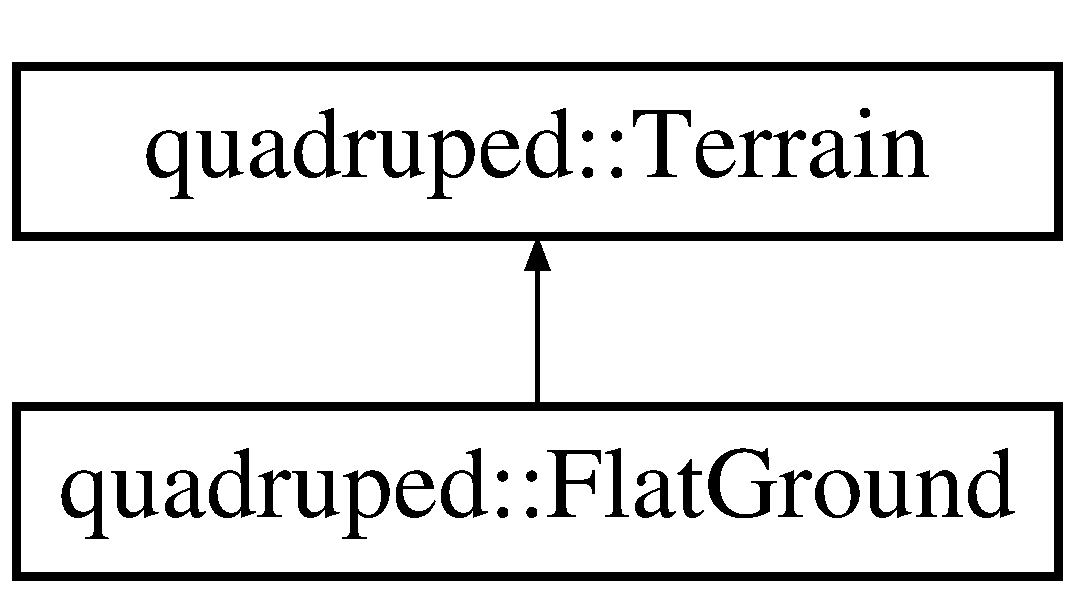
\includegraphics[height=2.000000cm]{classquadruped_1_1FlatGround}
\end{center}
\end{figure}
\subsection*{Public 成员函数}
\begin{DoxyCompactItemize}
\item 
\mbox{\Hypertarget{classquadruped_1_1FlatGround_af6fe169b0875a48a568b2f9dc0b374ac}\label{classquadruped_1_1FlatGround_af6fe169b0875a48a568b2f9dc0b374ac}} 
\hyperlink{classquadruped_1_1FlatGround_af6fe169b0875a48a568b2f9dc0b374ac}{Flat\+Ground} (void)
\begin{DoxyCompactList}\small\item\em Flat\+Ground类的构造函数，完成地形标识符以及地形分割线的初始化 \end{DoxyCompactList}\item 
virtual double \hyperlink{classquadruped_1_1FlatGround_a26e906052e0b42eef3b142e13aa55d9e}{Get\+Hight} (double p\+\_\+x, double p\+\_\+y) override
\begin{DoxyCompactList}\small\item\em 获取当前地形在世界坐标系下的高度 \end{DoxyCompactList}\item 
virtual \hyperlink{cppTypes_8h_a65c27bf97693676535dd0b30ea0ad399}{Vec3}$<$ double $>$ \hyperlink{classquadruped_1_1FlatGround_a14e8cc9794ef3f8c1250e757b9cb0387}{Get\+Normal\+Vector} (double p\+\_\+x, double p\+\_\+y) override
\begin{DoxyCompactList}\small\item\em 获取当前地形在世界坐标系下的法向量 \end{DoxyCompactList}\end{DoxyCompactItemize}
\subsection*{额外继承的成员函数}


\subsection{详细描述}
平地类子类 

\subsection{成员函数说明}
\mbox{\Hypertarget{classquadruped_1_1FlatGround_a26e906052e0b42eef3b142e13aa55d9e}\label{classquadruped_1_1FlatGround_a26e906052e0b42eef3b142e13aa55d9e}} 
\index{quadruped\+::\+Flat\+Ground@{quadruped\+::\+Flat\+Ground}!Get\+Hight@{Get\+Hight}}
\index{Get\+Hight@{Get\+Hight}!quadruped\+::\+Flat\+Ground@{quadruped\+::\+Flat\+Ground}}
\subsubsection{\texorpdfstring{Get\+Hight()}{GetHight()}}
{\footnotesize\ttfamily double Flat\+Ground\+::\+Get\+Hight (\begin{DoxyParamCaption}\item[{double}]{p\+\_\+x,  }\item[{double}]{p\+\_\+y }\end{DoxyParamCaption})\hspace{0.3cm}{\ttfamily [override]}, {\ttfamily [virtual]}}



获取当前地形在世界坐标系下的高度 


\begin{DoxyParams}{参数}
{\em p\+\_\+x} & 当前点在世界坐标系位置坐标的\+X值 \\
\hline
{\em p\+\_\+y} & 当前点在世界坐标系位置坐标的\+Y值 \\
\hline
\end{DoxyParams}
\begin{DoxyReturn}{返回}
double 
\end{DoxyReturn}


重载 \hyperlink{classquadruped_1_1Terrain}{quadruped\+::\+Terrain} .

\mbox{\Hypertarget{classquadruped_1_1FlatGround_a14e8cc9794ef3f8c1250e757b9cb0387}\label{classquadruped_1_1FlatGround_a14e8cc9794ef3f8c1250e757b9cb0387}} 
\index{quadruped\+::\+Flat\+Ground@{quadruped\+::\+Flat\+Ground}!Get\+Normal\+Vector@{Get\+Normal\+Vector}}
\index{Get\+Normal\+Vector@{Get\+Normal\+Vector}!quadruped\+::\+Flat\+Ground@{quadruped\+::\+Flat\+Ground}}
\subsubsection{\texorpdfstring{Get\+Normal\+Vector()}{GetNormalVector()}}
{\footnotesize\ttfamily \hyperlink{cppTypes_8h_a65c27bf97693676535dd0b30ea0ad399}{Vec3}$<$ double $>$ Flat\+Ground\+::\+Get\+Normal\+Vector (\begin{DoxyParamCaption}\item[{double}]{p\+\_\+x,  }\item[{double}]{p\+\_\+y }\end{DoxyParamCaption})\hspace{0.3cm}{\ttfamily [override]}, {\ttfamily [virtual]}}



获取当前地形在世界坐标系下的法向量 


\begin{DoxyParams}{参数}
{\em p\+\_\+x} & 当前点在世界坐标系位置坐标的\+X值 \\
\hline
{\em p\+\_\+y} & 当前点在世界坐标系位置坐标的\+Y值 \\
\hline
\end{DoxyParams}
\begin{DoxyReturn}{返回}
Vec3$<$double$>$ 
\end{DoxyReturn}


实现了 \hyperlink{classquadruped_1_1Terrain}{quadruped\+::\+Terrain}.



该类的文档由以下文件生成\+:\begin{DoxyCompactItemize}
\item 
controller/motion\+Plan/terrain/\hyperlink{terrain_8hpp}{terrain.\+hpp}\item 
controller/motion\+Plan/terrain/\hyperlink{terrain_8cpp}{terrain.\+cpp}\end{DoxyCompactItemize}

\hypertarget{classquadruped_1_1FloatingBaseModel}{}\section{quadruped\+:\+:Floating\+Base\+Model类 参考}
\label{classquadruped_1_1FloatingBaseModel}\index{quadruped\+::\+Floating\+Base\+Model@{quadruped\+::\+Floating\+Base\+Model}}
\subsection*{Public 成员函数}
\begin{DoxyCompactItemize}
\item 
\mbox{\Hypertarget{classquadruped_1_1FloatingBaseModel_a5f5f04261e961fae57f84aaf80f65f4f}\label{classquadruped_1_1FloatingBaseModel_a5f5f04261e961fae57f84aaf80f65f4f}} 
bool {\bfseries get\+Mass\+Inertia} (dynacore\+::\+Matrix \&A) const
\item 
\mbox{\Hypertarget{classquadruped_1_1FloatingBaseModel_a7955bced1fbfb11965de500d31900d3d}\label{classquadruped_1_1FloatingBaseModel_a7955bced1fbfb11965de500d31900d3d}} 
bool {\bfseries get\+Inverse\+Mass\+Inertia} (dynacore\+::\+Matrix \&Ainv) const
\item 
\mbox{\Hypertarget{classquadruped_1_1FloatingBaseModel_a8f337459898a613548efb4af536f64e1}\label{classquadruped_1_1FloatingBaseModel_a8f337459898a613548efb4af536f64e1}} 
bool {\bfseries get\+Gravity} (dynacore\+::\+Vector \&grav) const
\item 
\mbox{\Hypertarget{classquadruped_1_1FloatingBaseModel_a5345ee06da415df56a17623a100addfe}\label{classquadruped_1_1FloatingBaseModel_a5345ee06da415df56a17623a100addfe}} 
bool {\bfseries get\+Coriolis} (dynacore\+::\+Vector \&coriolis) const
\item 
\mbox{\Hypertarget{classquadruped_1_1FloatingBaseModel_afb96803e722a8d0565f1a43327935b27}\label{classquadruped_1_1FloatingBaseModel_afb96803e722a8d0565f1a43327935b27}} 
void {\bfseries get\+Centroid\+Jacobian} (dynacore\+::\+Matrix \&Jcent) const
\item 
\mbox{\Hypertarget{classquadruped_1_1FloatingBaseModel_a16dcc8e6ed6984a0996d2d7648b0a351}\label{classquadruped_1_1FloatingBaseModel_a16dcc8e6ed6984a0996d2d7648b0a351}} 
void {\bfseries get\+Centroid\+Inertia} (dynacore\+::\+Matrix \&Icent) const
\item 
\mbox{\Hypertarget{classquadruped_1_1FloatingBaseModel_aa38322065e6fa0c7381b3a82874854e0}\label{classquadruped_1_1FloatingBaseModel_aa38322065e6fa0c7381b3a82874854e0}} 
void {\bfseries get\+Co\+M\+Position} (dynacore\+::\+Vect3 \&com\+\_\+pos) const
\item 
\mbox{\Hypertarget{classquadruped_1_1FloatingBaseModel_a10349bcc5d2bf90b5587773efab8cc44}\label{classquadruped_1_1FloatingBaseModel_a10349bcc5d2bf90b5587773efab8cc44}} 
void {\bfseries get\+Co\+M\+Velocity} (dynacore\+::\+Vect3 \&com\+\_\+vel) const
\item 
\mbox{\Hypertarget{classquadruped_1_1FloatingBaseModel_a6e7a003cb230a5ec8696c46a2047a6c0}\label{classquadruped_1_1FloatingBaseModel_a6e7a003cb230a5ec8696c46a2047a6c0}} 
void {\bfseries get\+Pos} (int link\+\_\+id, dynacore\+::\+Vect3 \&pos) const
\item 
\mbox{\Hypertarget{classquadruped_1_1FloatingBaseModel_ab66894859661648f90a2218a43ad0b01}\label{classquadruped_1_1FloatingBaseModel_ab66894859661648f90a2218a43ad0b01}} 
void {\bfseries get\+Ori} (int link\+\_\+id, dynacore\+::\+Vect3 \&rpy) const
\item 
\mbox{\Hypertarget{classquadruped_1_1FloatingBaseModel_a400825b773081cdd886383624d53b542}\label{classquadruped_1_1FloatingBaseModel_a400825b773081cdd886383624d53b542}} 
void {\bfseries get\+Linear\+Vel} (int link\+\_\+id, dynacore\+::\+Vect3 \&lin\+\_\+vel) const
\item 
\mbox{\Hypertarget{classquadruped_1_1FloatingBaseModel_a48efc47609ab056a82d0cc8bd882bf04}\label{classquadruped_1_1FloatingBaseModel_a48efc47609ab056a82d0cc8bd882bf04}} 
void {\bfseries get\+Angular\+Vel} (int link\+\_\+id, dynacore\+::\+Vect3 \&ang\+\_\+vel) const
\item 
\mbox{\Hypertarget{classquadruped_1_1FloatingBaseModel_ac94400de545c66a32020c4d3671ccff0}\label{classquadruped_1_1FloatingBaseModel_ac94400de545c66a32020c4d3671ccff0}} 
void {\bfseries get\+Centroid\+Velocity} (dynacore\+::\+Vector \&centroid\+\_\+vel) const
\item 
\mbox{\Hypertarget{classquadruped_1_1FloatingBaseModel_a1b0c2f3c829e2544edb507a5934411f6}\label{classquadruped_1_1FloatingBaseModel_a1b0c2f3c829e2544edb507a5934411f6}} 
void {\bfseries get\+Co\+M\+Jacobian} (dynacore\+::\+Matrix \&J) const
\item 
\mbox{\Hypertarget{classquadruped_1_1FloatingBaseModel_a4076657aec4909dc3e2cda3dd57ba701}\label{classquadruped_1_1FloatingBaseModel_a4076657aec4909dc3e2cda3dd57ba701}} 
void {\bfseries get\+Full\+Jacobian} (int link\+\_\+id, dynacore\+::\+Matrix \&J) const
\item 
\mbox{\Hypertarget{classquadruped_1_1FloatingBaseModel_a0a1208545b05039a0e5ced7dfa90a9ae}\label{classquadruped_1_1FloatingBaseModel_a0a1208545b05039a0e5ced7dfa90a9ae}} 
void {\bfseries get\+Full\+J\+Dot\+Qdot} (int link\+\_\+id, dynacore\+::\+Vector \&J\+Dot\+Qdot) const
\item 
\mbox{\Hypertarget{classquadruped_1_1FloatingBaseModel_a69cddd67f824106ba6701543cac5aa59}\label{classquadruped_1_1FloatingBaseModel_a69cddd67f824106ba6701543cac5aa59}} 
void {\bfseries get\+World2\+Body\+Matrix} (\hyperlink{cppTypes_8h_adb7d462b35d31f0b2583b3e230a2a2c3}{dynacore\+::\+Mat3} \&\+\_\+\+World2\+Body)
\item 
\mbox{\Hypertarget{classquadruped_1_1FloatingBaseModel_aeb288572af74c8f33301278db6457df6}\label{classquadruped_1_1FloatingBaseModel_aeb288572af74c8f33301278db6457df6}} 
void {\bfseries Update\+System} (const dynacore\+::\+Vector \&q, const dynacore\+::\+Vector \&qdot)
\item 
\mbox{\Hypertarget{classquadruped_1_1FloatingBaseModel_a64aa3de0bde270639f9d8ae15e14a6da}\label{classquadruped_1_1FloatingBaseModel_a64aa3de0bde270639f9d8ae15e14a6da}} 
void {\bfseries Print\+Link\+List} ()
\item 
\mbox{\Hypertarget{classquadruped_1_1FloatingBaseModel_a528aa7164d4ddae2023d42ee800d0daa}\label{classquadruped_1_1FloatingBaseModel_a528aa7164d4ddae2023d42ee800d0daa}} 
unsigned int {\bfseries Find\+Link\+Id} (const char $\ast$link\+\_\+name)
\end{DoxyCompactItemize}
\subsection*{Public 属性}
\begin{DoxyCompactItemize}
\item 
\mbox{\Hypertarget{classquadruped_1_1FloatingBaseModel_ac660e406ae345554214e1fb8a4ae306c}\label{classquadruped_1_1FloatingBaseModel_ac660e406ae345554214e1fb8a4ae306c}} 
Rigid\+Body\+Dynamics\+::\+Model $\ast$ {\bfseries model\+\_\+}
\end{DoxyCompactItemize}
\subsection*{Protected 属性}
\begin{DoxyCompactItemize}
\item 
\mbox{\Hypertarget{classquadruped_1_1FloatingBaseModel_ad202e2949cc99f2db21a96e23018fdc3}\label{classquadruped_1_1FloatingBaseModel_ad202e2949cc99f2db21a96e23018fdc3}} 
\hyperlink{classquadruped_1_1DynModel}{Dyn\+Model} $\ast$ {\bfseries dyn\+\_\+model\+\_\+}
\item 
\mbox{\Hypertarget{classquadruped_1_1FloatingBaseModel_a1baa9dc5905af1e90b0c86bc9b88bc76}\label{classquadruped_1_1FloatingBaseModel_a1baa9dc5905af1e90b0c86bc9b88bc76}} 
\hyperlink{classquadruped_1_1KinModel}{Kin\+Model} $\ast$ {\bfseries kin\+\_\+model\+\_\+}
\end{DoxyCompactItemize}


该类的文档由以下文件生成\+:\begin{DoxyCompactItemize}
\item 
controller/model/floating\+Base\+Model.\+hpp\item 
controller/model/floating\+Base\+Model.\+cpp\end{DoxyCompactItemize}

\hypertarget{classquadruped_1_1Foothold}{}\section{quadruped\+:\+:Foothold类 参考}
\label{classquadruped_1_1Foothold}\index{quadruped\+::\+Foothold@{quadruped\+::\+Foothold}}
\subsection*{Public 成员函数}
\begin{DoxyCompactItemize}
\item 
\hyperlink{classquadruped_1_1Foothold_ac819b1b86d952ee70953e0f03444ac2a}{Foothold} (\hyperlink{classquadruped_1_1Parameters}{Parameters} $\ast$p\+\_\+para, \hyperlink{classquadruped_1_1Terrain}{Terrain} $\ast$p\+\_\+terrain\+\_\+now)
\item 
void \hyperlink{classquadruped_1_1Foothold_a3731827dcb2f4e75e3ff701f0b04d962}{Get\+Foot\+Hold} (void)
\end{DoxyCompactItemize}
\subsection*{Public 属性}
\begin{DoxyCompactItemize}
\item 
\mbox{\Hypertarget{classquadruped_1_1Foothold_a6158308a079a360f4d92a5ee619f1cdb}\label{classquadruped_1_1Foothold_a6158308a079a360f4d92a5ee619f1cdb}} 
\hyperlink{classquadruped_1_1FH__updataInfo}{F\+H\+\_\+updata\+Info} $\ast$ {\bfseries updata\+Info}
\item 
\mbox{\Hypertarget{classquadruped_1_1Foothold_a2bd27fdd1d09e8b75cde6ffe41f15c56}\label{classquadruped_1_1Foothold_a2bd27fdd1d09e8b75cde6ffe41f15c56}} 
Smart\+Ptr$<$ T\+N\+LP $>$ {\bfseries f\+H\+\_\+nlp}
\end{DoxyCompactItemize}


\subsection{构造及析构函数说明}
\mbox{\Hypertarget{classquadruped_1_1Foothold_ac819b1b86d952ee70953e0f03444ac2a}\label{classquadruped_1_1Foothold_ac819b1b86d952ee70953e0f03444ac2a}} 
\index{quadruped\+::\+Foothold@{quadruped\+::\+Foothold}!Foothold@{Foothold}}
\index{Foothold@{Foothold}!quadruped\+::\+Foothold@{quadruped\+::\+Foothold}}
\subsubsection{\texorpdfstring{Foothold()}{Foothold()}}
{\footnotesize\ttfamily Foothold\+::\+Foothold (\begin{DoxyParamCaption}\item[{\hyperlink{classquadruped_1_1Parameters}{Parameters} $\ast$}]{p\+\_\+para,  }\item[{\hyperlink{classquadruped_1_1Terrain}{Terrain} $\ast$}]{p\+\_\+terrain\+\_\+now }\end{DoxyParamCaption})\hspace{0.3cm}{\ttfamily [explicit]}}

\+: 配置落足点规划中的ipopt求解器 
\begin{DoxyParams}{参数}
{\em \{\+Parameters$\ast$\}} & p\+\_\+para \\
\hline
{\em \{\+Terrain$\ast$\}} & p\+\_\+terrain\+\_\+now \\
\hline
\end{DoxyParams}
\begin{DoxyReturn}{返回}
\{$\ast$\} 
\end{DoxyReturn}


\subsection{成员函数说明}
\mbox{\Hypertarget{classquadruped_1_1Foothold_a3731827dcb2f4e75e3ff701f0b04d962}\label{classquadruped_1_1Foothold_a3731827dcb2f4e75e3ff701f0b04d962}} 
\index{quadruped\+::\+Foothold@{quadruped\+::\+Foothold}!Get\+Foot\+Hold@{Get\+Foot\+Hold}}
\index{Get\+Foot\+Hold@{Get\+Foot\+Hold}!quadruped\+::\+Foothold@{quadruped\+::\+Foothold}}
\subsubsection{\texorpdfstring{Get\+Foot\+Hold()}{GetFootHold()}}
{\footnotesize\ttfamily void Foothold\+::\+Get\+Foot\+Hold (\begin{DoxyParamCaption}\item[{void}]{ }\end{DoxyParamCaption})}

\+: 通过求解非线性规划问题得到落足点 
\begin{DoxyParams}{参数}
{\em \{$\ast$\}} & \\
\hline
\end{DoxyParams}
\begin{DoxyReturn}{返回}
\{$\ast$\} 
\end{DoxyReturn}


该类的文档由以下文件生成\+:\begin{DoxyCompactItemize}
\item 
controller/motion\+Plan/foothold/foothold.\+hpp\item 
controller/motion\+Plan/foothold/foothold.\+cpp\end{DoxyCompactItemize}

\hypertarget{classquadruped_1_1Gamepad}{}\section{quadruped\+:\+:Gamepad类 参考}
\label{classquadruped_1_1Gamepad}\index{quadruped\+::\+Gamepad@{quadruped\+::\+Gamepad}}


Actiger遥控器类  




{\ttfamily \#include $<$gamepad.\+hpp$>$}

\subsection*{Public 成员函数}
\begin{DoxyCompactItemize}
\item 
\mbox{\Hypertarget{classquadruped_1_1Gamepad_a299e3657b0c2a2d0252d307808e1b5d5}\label{classquadruped_1_1Gamepad_a299e3657b0c2a2d0252d307808e1b5d5}} 
\hyperlink{classquadruped_1_1Gamepad_a299e3657b0c2a2d0252d307808e1b5d5}{Gamepad} (void)
\begin{DoxyCompactList}\small\item\em Gamepad类的构造函数，完成硬件的读取 \end{DoxyCompactList}\item 
\mbox{\Hypertarget{classquadruped_1_1Gamepad_afde709704acc2d1219758ed25004adfd}\label{classquadruped_1_1Gamepad_afde709704acc2d1219758ed25004adfd}} 
virtual \hyperlink{classquadruped_1_1Gamepad_afde709704acc2d1219758ed25004adfd}{$\sim$\+Gamepad} (void)
\begin{DoxyCompactList}\small\item\em Gamepad类的析构函数 \end{DoxyCompactList}\item 
int \hyperlink{classquadruped_1_1Gamepad_a45193124f6e45a794fff7770d48bb1c4}{xbox\+\_\+open} (const char $\ast$file\+\_\+name)
\begin{DoxyCompactList}\small\item\em 打开遥控器 \end{DoxyCompactList}\item 
int \hyperlink{classquadruped_1_1Gamepad_a0a3c2f9e2e580af60d3d961cd7c961f5}{xbox\+\_\+map\+\_\+read} (int xbox\+\_\+fd, \hyperlink{structxbox__map__t}{xbox\+\_\+map\+\_\+t} $\ast$p\+\_\+map)
\begin{DoxyCompactList}\small\item\em 读取遥控器按键状态并完成键值映射 \end{DoxyCompactList}\item 
void \hyperlink{classquadruped_1_1Gamepad_aedbe5a93bd4af4b3fb22137ae1549612}{xbox\+\_\+close} (int xbox\+\_\+fd)
\begin{DoxyCompactList}\small\item\em 关闭遥控器 \end{DoxyCompactList}\item 
void \hyperlink{classquadruped_1_1Gamepad_a2231f881a5ce074c07520781b01bf364}{Get\+Key} (uint8\+\_\+t $\ast$p\+\_\+gait\+Now)
\begin{DoxyCompactList}\small\item\em 根据遥控器映射的键值完成状态标志位的转换 \end{DoxyCompactList}\end{DoxyCompactItemize}
\subsection*{Public 属性}
\begin{DoxyCompactItemize}
\item 
\mbox{\Hypertarget{classquadruped_1_1Gamepad_a1c1056b8a615214ad8e4d4e03ffb1962}\label{classquadruped_1_1Gamepad_a1c1056b8a615214ad8e4d4e03ffb1962}} 
\hyperlink{structxbox__map__t}{xbox\+\_\+map\+\_\+t} \hyperlink{classquadruped_1_1Gamepad_a1c1056b8a615214ad8e4d4e03ffb1962}{map}
\begin{DoxyCompactList}\small\item\em 遥控器键值映射结构体成员 \end{DoxyCompactList}\end{DoxyCompactItemize}


\subsection{详细描述}
Actiger遥控器类 

\subsection{成员函数说明}
\mbox{\Hypertarget{classquadruped_1_1Gamepad_a2231f881a5ce074c07520781b01bf364}\label{classquadruped_1_1Gamepad_a2231f881a5ce074c07520781b01bf364}} 
\index{quadruped\+::\+Gamepad@{quadruped\+::\+Gamepad}!Get\+Key@{Get\+Key}}
\index{Get\+Key@{Get\+Key}!quadruped\+::\+Gamepad@{quadruped\+::\+Gamepad}}
\subsubsection{\texorpdfstring{Get\+Key()}{GetKey()}}
{\footnotesize\ttfamily void Gamepad\+::\+Get\+Key (\begin{DoxyParamCaption}\item[{uint8\+\_\+t $\ast$}]{p\+\_\+gait\+Now }\end{DoxyParamCaption})}



根据遥控器映射的键值完成状态标志位的转换 


\begin{DoxyParams}{参数}
{\em p\+\_\+gait\+Now} & Actiger当前的步态 \\
\hline
\end{DoxyParams}


参考 handle, I\+N\+I\+T\+\_\+\+H\+E\+I\+G\+HT, handle\+\_\+t\+::stand\+Ready , 以及 handle\+\_\+t\+::step\+Over.



参考自 Motion\+Plan\+Run().

\mbox{\Hypertarget{classquadruped_1_1Gamepad_aedbe5a93bd4af4b3fb22137ae1549612}\label{classquadruped_1_1Gamepad_aedbe5a93bd4af4b3fb22137ae1549612}} 
\index{quadruped\+::\+Gamepad@{quadruped\+::\+Gamepad}!xbox\+\_\+close@{xbox\+\_\+close}}
\index{xbox\+\_\+close@{xbox\+\_\+close}!quadruped\+::\+Gamepad@{quadruped\+::\+Gamepad}}
\subsubsection{\texorpdfstring{xbox\+\_\+close()}{xbox\_close()}}
{\footnotesize\ttfamily void Gamepad\+::xbox\+\_\+close (\begin{DoxyParamCaption}\item[{int}]{xbox\+\_\+fd }\end{DoxyParamCaption})}



关闭遥控器 


\begin{DoxyParams}{参数}
{\em xbox\+\_\+fd} & 设备文件 \\
\hline
\end{DoxyParams}
\mbox{\Hypertarget{classquadruped_1_1Gamepad_a0a3c2f9e2e580af60d3d961cd7c961f5}\label{classquadruped_1_1Gamepad_a0a3c2f9e2e580af60d3d961cd7c961f5}} 
\index{quadruped\+::\+Gamepad@{quadruped\+::\+Gamepad}!xbox\+\_\+map\+\_\+read@{xbox\+\_\+map\+\_\+read}}
\index{xbox\+\_\+map\+\_\+read@{xbox\+\_\+map\+\_\+read}!quadruped\+::\+Gamepad@{quadruped\+::\+Gamepad}}
\subsubsection{\texorpdfstring{xbox\+\_\+map\+\_\+read()}{xbox\_map\_read()}}
{\footnotesize\ttfamily int Gamepad\+::xbox\+\_\+map\+\_\+read (\begin{DoxyParamCaption}\item[{int}]{xbox\+\_\+fd,  }\item[{\hyperlink{structxbox__map__t}{xbox\+\_\+map\+\_\+t} $\ast$}]{p\+\_\+map }\end{DoxyParamCaption})}



读取遥控器按键状态并完成键值映射 


\begin{DoxyParams}{参数}
{\em xbox\+\_\+fd} & 设备文件 \\
\hline
{\em p\+\_\+map} & 键值映射结构体 \\
\hline
\end{DoxyParams}
\begin{DoxyReturn}{返回}
int 
\end{DoxyReturn}


参考 X\+B\+O\+X\+\_\+\+A\+X\+I\+S\+\_\+\+LX, X\+B\+O\+X\+\_\+\+A\+X\+I\+S\+\_\+\+LY, X\+B\+O\+X\+\_\+\+A\+X\+I\+S\+\_\+\+RX, X\+B\+O\+X\+\_\+\+A\+X\+I\+S\+\_\+\+RY, X\+B\+O\+X\+\_\+\+B\+U\+T\+T\+O\+N\+\_\+A, X\+B\+O\+X\+\_\+\+B\+U\+T\+T\+O\+N\+\_\+B, X\+B\+O\+X\+\_\+\+B\+U\+T\+T\+O\+N\+\_\+\+D\+O\+WN, X\+B\+O\+X\+\_\+\+B\+U\+T\+T\+O\+N\+\_\+\+H\+O\+ME, X\+B\+O\+X\+\_\+\+B\+U\+T\+T\+O\+N\+\_\+L, X\+B\+O\+X\+\_\+\+B\+U\+T\+T\+O\+N\+\_\+\+L\+E\+FT, X\+B\+O\+X\+\_\+\+B\+U\+T\+T\+O\+N\+\_\+\+LO, X\+B\+O\+X\+\_\+\+B\+U\+T\+T\+O\+N\+\_\+\+LZ, X\+B\+O\+X\+\_\+\+B\+U\+T\+T\+O\+N\+\_\+\+M\+I\+N\+US, X\+B\+O\+X\+\_\+\+B\+U\+T\+T\+O\+N\+\_\+\+P\+L\+US, X\+B\+O\+X\+\_\+\+B\+U\+T\+T\+O\+N\+\_\+R, X\+B\+O\+X\+\_\+\+B\+U\+T\+T\+O\+N\+\_\+\+R\+I\+G\+HT, X\+B\+O\+X\+\_\+\+B\+U\+T\+T\+O\+N\+\_\+\+RO, X\+B\+O\+X\+\_\+\+B\+U\+T\+T\+O\+N\+\_\+\+RZ, X\+B\+O\+X\+\_\+\+B\+U\+T\+T\+O\+N\+\_\+\+UP, X\+B\+O\+X\+\_\+\+B\+U\+T\+T\+O\+N\+\_\+X , 以及 X\+B\+O\+X\+\_\+\+B\+U\+T\+T\+O\+N\+\_\+Y.

\mbox{\Hypertarget{classquadruped_1_1Gamepad_a45193124f6e45a794fff7770d48bb1c4}\label{classquadruped_1_1Gamepad_a45193124f6e45a794fff7770d48bb1c4}} 
\index{quadruped\+::\+Gamepad@{quadruped\+::\+Gamepad}!xbox\+\_\+open@{xbox\+\_\+open}}
\index{xbox\+\_\+open@{xbox\+\_\+open}!quadruped\+::\+Gamepad@{quadruped\+::\+Gamepad}}
\subsubsection{\texorpdfstring{xbox\+\_\+open()}{xbox\_open()}}
{\footnotesize\ttfamily int Gamepad\+::xbox\+\_\+open (\begin{DoxyParamCaption}\item[{const char $\ast$}]{file\+\_\+name }\end{DoxyParamCaption})}



打开遥控器 


\begin{DoxyParams}{参数}
{\em file\+\_\+name} & 设备文件 \\
\hline
\end{DoxyParams}
\begin{DoxyReturn}{返回}
int 
\end{DoxyReturn}


该类的文档由以下文件生成\+:\begin{DoxyCompactItemize}
\item 
controller/motion\+Plan/\hyperlink{gamepad_8hpp}{gamepad.\+hpp}\item 
controller/motion\+Plan/gamepad.\+cpp\end{DoxyCompactItemize}

\hypertarget{structhandle__t}{}\section{handle\+\_\+t结构体 参考}
\label{structhandle__t}\index{handle\+\_\+t@{handle\+\_\+t}}


标志位结构体  




{\ttfamily \#include $<$cpp\+Struct.\+h$>$}

\subsection*{Public 属性}
\begin{DoxyCompactItemize}
\item 
\mbox{\Hypertarget{structhandle__t_a9b8437a0a8457da1d58c0c3bcd794734}\label{structhandle__t_a9b8437a0a8457da1d58c0c3bcd794734}} 
bool {\bfseries start}
\item 
\mbox{\Hypertarget{structhandle__t_ad4ea92fd72901046c05b9ebfcc068f22}\label{structhandle__t_ad4ea92fd72901046c05b9ebfcc068f22}} 
bool {\bfseries unlock}
\item 
\mbox{\Hypertarget{structhandle__t_adf84a1e20d4ea39644a4e7731474e769}\label{structhandle__t_adf84a1e20d4ea39644a4e7731474e769}} 
uint8\+\_\+t {\bfseries terrain}
\item 
\mbox{\Hypertarget{structhandle__t_a99d1178b7440a0cff42eae05db115b98}\label{structhandle__t_a99d1178b7440a0cff42eae05db115b98}} 
double {\bfseries x\+\_\+speed}
\item 
\mbox{\Hypertarget{structhandle__t_a9bcac00bdfba0c0a8c195840d3f19a24}\label{structhandle__t_a9bcac00bdfba0c0a8c195840d3f19a24}} 
double {\bfseries y\+\_\+speed}
\item 
\mbox{\Hypertarget{structhandle__t_ab7295e8d71f5c5f0eb1026a69e65eed9}\label{structhandle__t_ab7295e8d71f5c5f0eb1026a69e65eed9}} 
double {\bfseries z\+\_\+height}
\item 
\mbox{\Hypertarget{structhandle__t_a5996e395d20efcfe338ee46b6c966642}\label{structhandle__t_a5996e395d20efcfe338ee46b6c966642}} 
double {\bfseries yaw\+\_\+omega}
\item 
\mbox{\Hypertarget{structhandle__t_a50a967933dfe95e52d18e382d63d5438}\label{structhandle__t_a50a967933dfe95e52d18e382d63d5438}} 
double {\bfseries s\+\_\+yaw}
\item 
\mbox{\Hypertarget{structhandle__t_aee9f102b30cf45e3f75ce546b5118f2f}\label{structhandle__t_aee9f102b30cf45e3f75ce546b5118f2f}} 
double {\bfseries s\+\_\+pitch}
\item 
\mbox{\Hypertarget{structhandle__t_a53d78dacc1f3171b0b9e2794cf7a8419}\label{structhandle__t_a53d78dacc1f3171b0b9e2794cf7a8419}} 
double {\bfseries s\+\_\+roll}
\item 
\mbox{\Hypertarget{structhandle__t_a0dc631dba1dda177f48aeb01c7e9570c}\label{structhandle__t_a0dc631dba1dda177f48aeb01c7e9570c}} 
bool \hyperlink{structhandle__t_a0dc631dba1dda177f48aeb01c7e9570c}{stand\+Ready}
\begin{DoxyCompactList}\small\item\em 站立完成的标志位 \end{DoxyCompactList}\item 
\mbox{\Hypertarget{structhandle__t_ad2325b25d45a792fc3270916f2d84e1c}\label{structhandle__t_ad2325b25d45a792fc3270916f2d84e1c}} 
bool \hyperlink{structhandle__t_ad2325b25d45a792fc3270916f2d84e1c}{step\+Over}
\begin{DoxyCompactList}\small\item\em 一步转换完成的标志位 \end{DoxyCompactList}\item 
\mbox{\Hypertarget{structhandle__t_a2873f23ea50d990fc9cd6b9bcc83c0cb}\label{structhandle__t_a2873f23ea50d990fc9cd6b9bcc83c0cb}} 
bool \hyperlink{structhandle__t_a2873f23ea50d990fc9cd6b9bcc83c0cb}{is\+\_\+lf\+\_\+rr\+\_\+stand}
\begin{DoxyCompactList}\small\item\em 判断支撑腿的标志位 \end{DoxyCompactList}\end{DoxyCompactItemize}


\subsection{详细描述}
标志位结构体 

该结构体的文档由以下文件生成\+:\begin{DoxyCompactItemize}
\item 
\hyperlink{cppStruct_8h}{cpp\+Struct.\+h}\end{DoxyCompactItemize}

\hypertarget{classquadruped_1_1Hurdles}{}\section{quadruped\+:\+:Hurdles类 参考}
\label{classquadruped_1_1Hurdles}\index{quadruped\+::\+Hurdles@{quadruped\+::\+Hurdles}}
类 quadruped\+:\+:Hurdles 继承关系图\+:\begin{figure}[H]
\begin{center}
\leavevmode
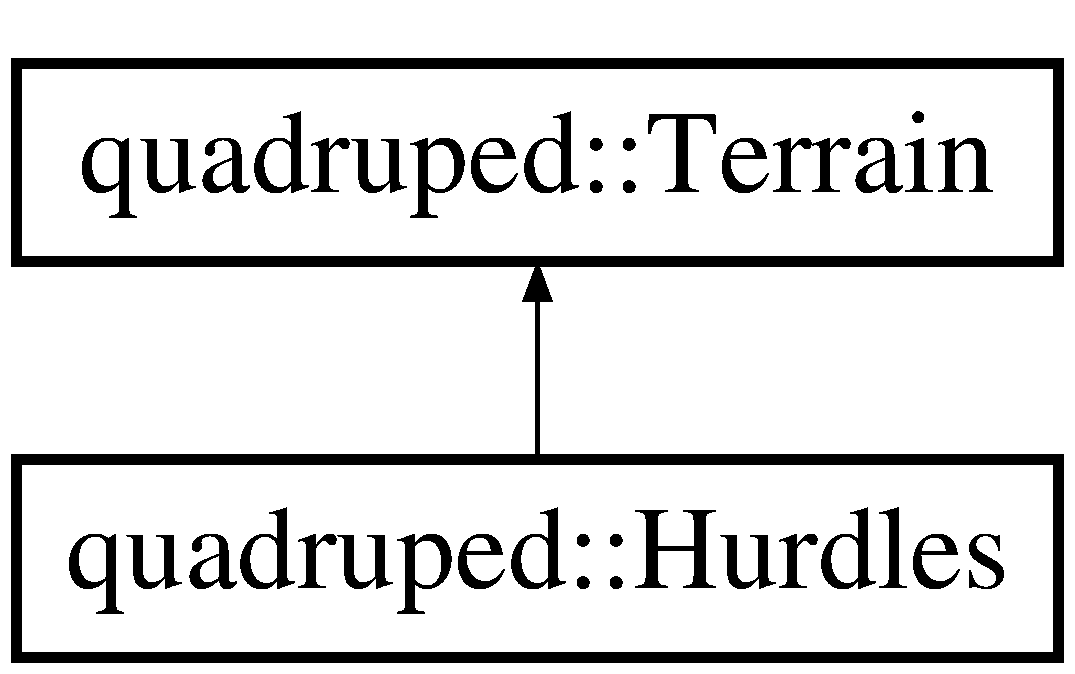
\includegraphics[height=2.000000cm]{classquadruped_1_1Hurdles}
\end{center}
\end{figure}
\subsection*{Public 成员函数}
\begin{DoxyCompactItemize}
\item 
\mbox{\Hypertarget{classquadruped_1_1Hurdles_a1df7dbe5b32d32cb41bf6cfa5acce288}\label{classquadruped_1_1Hurdles_a1df7dbe5b32d32cb41bf6cfa5acce288}} 
virtual double {\bfseries Get\+Hight} (double p\+\_\+x, double p\+\_\+y) override
\item 
\mbox{\Hypertarget{classquadruped_1_1Hurdles_adeec44aa28a458804b8acef478b590f0}\label{classquadruped_1_1Hurdles_adeec44aa28a458804b8acef478b590f0}} 
virtual void {\bfseries Updata\+Edge} (double p\+\_\+first\+\_\+edge\+\_\+\+D\+\_\+x, double p\+\_\+first\+\_\+edge\+\_\+\+D\+\_\+y) override
\item 
\mbox{\Hypertarget{classquadruped_1_1Hurdles_aa9bc6242d69aff7730202a57541f84f0}\label{classquadruped_1_1Hurdles_aa9bc6242d69aff7730202a57541f84f0}} 
virtual \hyperlink{cppTypes_8h_a65c27bf97693676535dd0b30ea0ad399}{Vec3}$<$ double $>$ {\bfseries Get\+Normal\+Vector} (double p\+\_\+x, double p\+\_\+y) override
\end{DoxyCompactItemize}
\subsection*{额外继承的成员函数}


该类的文档由以下文件生成\+:\begin{DoxyCompactItemize}
\item 
controller/motion\+Plan/terrain/\hyperlink{terrain_8hpp}{terrain.\+hpp}\item 
controller/motion\+Plan/terrain/\hyperlink{terrain_8cpp}{terrain.\+cpp}\end{DoxyCompactItemize}

\hypertarget{structimu__t}{}\section{imu\+\_\+t结构体 参考}
\label{structimu__t}\index{imu\+\_\+t@{imu\+\_\+t}}


I\+M\+U信息结构体：欧拉角 $\vert$ 欧拉角速度  




{\ttfamily \#include $<$cpp\+Struct.\+h$>$}

\subsection*{Public 属性}
\begin{DoxyCompactItemize}
\item 
\mbox{\Hypertarget{structimu__t_a18d3387cf594617f68400f22e5048e3b}\label{structimu__t_a18d3387cf594617f68400f22e5048e3b}} 
float {\bfseries pitch}
\item 
\mbox{\Hypertarget{structimu__t_a594af68bc33544092bd05cef2f67014e}\label{structimu__t_a594af68bc33544092bd05cef2f67014e}} 
float {\bfseries roll}
\item 
\mbox{\Hypertarget{structimu__t_a8686ab1273593c7809c2d12f0c84d2c3}\label{structimu__t_a8686ab1273593c7809c2d12f0c84d2c3}} 
float {\bfseries yaw}
\item 
\mbox{\Hypertarget{structimu__t_a90fe5dabdf8cba9f13049081dfde646e}\label{structimu__t_a90fe5dabdf8cba9f13049081dfde646e}} 
float {\bfseries omega\+\_\+pitch}
\item 
\mbox{\Hypertarget{structimu__t_a4428695e46594503cfe1c5f7fae4c028}\label{structimu__t_a4428695e46594503cfe1c5f7fae4c028}} 
float {\bfseries omega\+\_\+roll}
\item 
\mbox{\Hypertarget{structimu__t_aede25d64148a000c47c6d2d80366f95c}\label{structimu__t_aede25d64148a000c47c6d2d80366f95c}} 
float {\bfseries omega\+\_\+yaw}
\end{DoxyCompactItemize}


\subsection{详细描述}
I\+M\+U信息结构体：欧拉角 $\vert$ 欧拉角速度 

该结构体的文档由以下文件生成\+:\begin{DoxyCompactItemize}
\item 
\hyperlink{cppStruct_8h}{cpp\+Struct.\+h}\end{DoxyCompactItemize}

\hypertarget{classKalmanFilterForVE}{}\section{Kalman\+Filter\+For\+V\+E类 参考}
\label{classKalmanFilterForVE}\index{Kalman\+Filter\+For\+VE@{Kalman\+Filter\+For\+VE}}
\subsection*{Public 成员函数}
\begin{DoxyCompactItemize}
\item 
\mbox{\Hypertarget{classKalmanFilterForVE_a483a5fbe53a03b1ac833276073c5c5e3}\label{classKalmanFilterForVE_a483a5fbe53a03b1ac833276073c5c5e3}} 
{\bfseries Kalman\+Filter\+For\+VE} (double mass\+\_\+input, double period\+\_\+input)
\item 
\mbox{\Hypertarget{classKalmanFilterForVE_a7e07280c92f48046446b5631704b635e}\label{classKalmanFilterForVE_a7e07280c92f48046446b5631704b635e}} 
void {\bfseries Cal\+Stddev\+Xdot} (std\+::vector$<$ bool $>$ contactlist\+\_\+input, int contact\+\_\+num\+\_\+input, \hyperlink{cppTypes_8h_a65c27bf97693676535dd0b30ea0ad399}{Vec3}$<$ double $>$ b\+\_\+xdot\+\_\+lf\+\_\+input, \hyperlink{cppTypes_8h_a65c27bf97693676535dd0b30ea0ad399}{Vec3}$<$ double $>$ b\+\_\+xdot\+\_\+lr\+\_\+input, \hyperlink{cppTypes_8h_a65c27bf97693676535dd0b30ea0ad399}{Vec3}$<$ double $>$ b\+\_\+xdot\+\_\+rf\+\_\+input, \hyperlink{cppTypes_8h_a65c27bf97693676535dd0b30ea0ad399}{Vec3}$<$ double $>$ b\+\_\+xdot\+\_\+rr\+\_\+input)
\item 
\mbox{\Hypertarget{classKalmanFilterForVE_a267337aec97d41f3c722aac5d14b09b4}\label{classKalmanFilterForVE_a267337aec97d41f3c722aac5d14b09b4}} 
void {\bfseries Cal\+Fz\+Average} (std\+::vector$<$ bool $>$ contactlist\+\_\+input, int contact\+\_\+num\+\_\+input)
\item 
\mbox{\Hypertarget{classKalmanFilterForVE_abd2df23b17b1284474afad42cfa137eb}\label{classKalmanFilterForVE_abd2df23b17b1284474afad42cfa137eb}} 
void {\bfseries Make\+MatrixF} ()
\item 
\mbox{\Hypertarget{classKalmanFilterForVE_a7524faa6cd36f64edd3ff16d6da21851}\label{classKalmanFilterForVE_a7524faa6cd36f64edd3ff16d6da21851}} 
void {\bfseries Make\+VectorU} ()
\item 
\mbox{\Hypertarget{classKalmanFilterForVE_af5a75eae96ecc2216c73391c6d1bc51d}\label{classKalmanFilterForVE_af5a75eae96ecc2216c73391c6d1bc51d}} 
void {\bfseries State\+Predict} ()
\item 
\mbox{\Hypertarget{classKalmanFilterForVE_aac4cbc05791d48ce4db5c0792543b6ca}\label{classKalmanFilterForVE_aac4cbc05791d48ce4db5c0792543b6ca}} 
void {\bfseries Cov\+Predict} ()
\item 
\mbox{\Hypertarget{classKalmanFilterForVE_aeba0220a16a77d7242fd46fdac46a12c}\label{classKalmanFilterForVE_aeba0220a16a77d7242fd46fdac46a12c}} 
void {\bfseries Get\+Measurement\+Error} ()
\item 
\mbox{\Hypertarget{classKalmanFilterForVE_ab5f0573c67c441e4ab6601bc5b39a847}\label{classKalmanFilterForVE_ab5f0573c67c441e4ab6601bc5b39a847}} 
void {\bfseries GetK} ()
\item 
\mbox{\Hypertarget{classKalmanFilterForVE_ae0236f9ddaf1b50238629b625c12a710}\label{classKalmanFilterForVE_ae0236f9ddaf1b50238629b625c12a710}} 
void {\bfseries State\+Update} ()
\item 
\mbox{\Hypertarget{classKalmanFilterForVE_a4ac37ed6256c1a50a466dbd7e77001b1}\label{classKalmanFilterForVE_a4ac37ed6256c1a50a466dbd7e77001b1}} 
void {\bfseries Cov\+Update} ()
\item 
\mbox{\Hypertarget{classKalmanFilterForVE_a22c13294c1e43ed52ff9a48ee1398243}\label{classKalmanFilterForVE_a22c13294c1e43ed52ff9a48ee1398243}} 
void {\bfseries Init} (\hyperlink{cppTypes_8h_a65c27bf97693676535dd0b30ea0ad399}{Vec3}$<$ double $>$ v\+\_\+k\+\_\+1\+\_\+input, \hyperlink{cppTypes_8h_adad69baca3c77d5f991be5d3c063fea7}{D\+Vec}$<$ double $>$ f\+\_\+k\+\_\+input, \hyperlink{cppTypes_8h_adad69baca3c77d5f991be5d3c063fea7}{D\+Vec}$<$ double $>$ f\+\_\+k\+\_\+1\+\_\+input, \hyperlink{cppTypes_8h_a65c27bf97693676535dd0b30ea0ad399}{Vec3}$<$ double $>$ xdot\+\_\+input, \hyperlink{cppTypes_8h_a65c27bf97693676535dd0b30ea0ad399}{Vec3}$<$ double $>$ p\+\_\+k\+\_\+input, \hyperlink{cppTypes_8h_a65c27bf97693676535dd0b30ea0ad399}{Vec3}$<$ double $>$ p\+\_\+k\+\_\+1\+\_\+input, \hyperlink{cppTypes_8h_a65c27bf97693676535dd0b30ea0ad399}{Vec3}$<$ double $>$ a\+\_\+k\+\_\+1\+\_\+input)
\item 
\mbox{\Hypertarget{classKalmanFilterForVE_ac09058040d34c1dbe0832b377e9181d5}\label{classKalmanFilterForVE_ac09058040d34c1dbe0832b377e9181d5}} 
void {\bfseries Ready} (std\+::vector$<$ bool $>$ contactlist\+\_\+input, int contact\+\_\+num\+\_\+input, \hyperlink{cppTypes_8h_a65c27bf97693676535dd0b30ea0ad399}{Vec3}$<$ double $>$ b\+\_\+xdot\+\_\+lf\+\_\+input, \hyperlink{cppTypes_8h_a65c27bf97693676535dd0b30ea0ad399}{Vec3}$<$ double $>$ b\+\_\+xdot\+\_\+lr\+\_\+input, \hyperlink{cppTypes_8h_a65c27bf97693676535dd0b30ea0ad399}{Vec3}$<$ double $>$ b\+\_\+xdot\+\_\+rf\+\_\+input, \hyperlink{cppTypes_8h_a65c27bf97693676535dd0b30ea0ad399}{Vec3}$<$ double $>$ b\+\_\+xdot\+\_\+rr\+\_\+input)
\item 
\mbox{\Hypertarget{classKalmanFilterForVE_a7c65734f15b3d548cc1dded4955a3dce}\label{classKalmanFilterForVE_a7c65734f15b3d548cc1dded4955a3dce}} 
void {\bfseries Filter} ()
\item 
\mbox{\Hypertarget{classKalmanFilterForVE_a0cbaff2c7a4c8b5f8ab62e44c96c3275}\label{classKalmanFilterForVE_a0cbaff2c7a4c8b5f8ab62e44c96c3275}} 
\hyperlink{cppTypes_8h_a27bb8a600520708a5928332e4e52a92e}{Vec6}$<$ double $>$ {\bfseries Result} ()
\end{DoxyCompactItemize}
\subsection*{Public 属性}
\begin{DoxyCompactItemize}
\item 
\mbox{\Hypertarget{classKalmanFilterForVE_a13f36667fd13adc9df140afc721b2471}\label{classKalmanFilterForVE_a13f36667fd13adc9df140afc721b2471}} 
double {\bfseries alpha\+\_\+1}
\item 
\mbox{\Hypertarget{classKalmanFilterForVE_a940483cf6d541154c5a75766eeb3e4f9}\label{classKalmanFilterForVE_a940483cf6d541154c5a75766eeb3e4f9}} 
double {\bfseries alpha\+\_\+2}
\item 
\mbox{\Hypertarget{classKalmanFilterForVE_ae5aee1d62ed0103ea0f14ae60cd149bb}\label{classKalmanFilterForVE_ae5aee1d62ed0103ea0f14ae60cd149bb}} 
double {\bfseries std\+\_\+velocity\+\_\+contribution\+\_\+x}
\item 
\mbox{\Hypertarget{classKalmanFilterForVE_af4eb61437404079e177cfc65e2031efb}\label{classKalmanFilterForVE_af4eb61437404079e177cfc65e2031efb}} 
double {\bfseries std\+\_\+velocity\+\_\+contribution\+\_\+y}
\item 
\mbox{\Hypertarget{classKalmanFilterForVE_a1ca261dbf3a3ef0d6800e0226a3e4625}\label{classKalmanFilterForVE_a1ca261dbf3a3ef0d6800e0226a3e4625}} 
double {\bfseries std\+\_\+velocity\+\_\+contribution\+\_\+z}
\item 
\mbox{\Hypertarget{classKalmanFilterForVE_acd7508d05dc989a70c0157bb5784d782}\label{classKalmanFilterForVE_acd7508d05dc989a70c0157bb5784d782}} 
double {\bfseries Q\+\_\+pos\+\_\+x}
\item 
\mbox{\Hypertarget{classKalmanFilterForVE_a33e297573da7d7ad4081a14bc7711239}\label{classKalmanFilterForVE_a33e297573da7d7ad4081a14bc7711239}} 
double {\bfseries Q\+\_\+pos\+\_\+y}
\item 
\mbox{\Hypertarget{classKalmanFilterForVE_afbc45d59caf3fbdc3e5cb2f754014db4}\label{classKalmanFilterForVE_afbc45d59caf3fbdc3e5cb2f754014db4}} 
double {\bfseries Q\+\_\+pos\+\_\+z}
\item 
\mbox{\Hypertarget{classKalmanFilterForVE_a92ef545ae33155598cd27fb0d0337fab}\label{classKalmanFilterForVE_a92ef545ae33155598cd27fb0d0337fab}} 
double {\bfseries mass}
\item 
\mbox{\Hypertarget{classKalmanFilterForVE_a68abba388cb8e515b4aa4b91ee0841c9}\label{classKalmanFilterForVE_a68abba388cb8e515b4aa4b91ee0841c9}} 
double {\bfseries period}
\item 
\mbox{\Hypertarget{classKalmanFilterForVE_a4f1ab6feac1bc9f017f94e907c8b3fad}\label{classKalmanFilterForVE_a4f1ab6feac1bc9f017f94e907c8b3fad}} 
\hyperlink{cppTypes_8h_a7275f6cb9931f180383d67c9a0571cbd}{Mat6}$<$ double $>$ {\bfseries matrix\+\_\+F} = \hyperlink{cppTypes_8h_a7275f6cb9931f180383d67c9a0571cbd}{Mat6}$<$double$>$\+::Zero(6, 6)
\item 
\mbox{\Hypertarget{classKalmanFilterForVE_a8a34b544f3c79a2cae72c4897979c649}\label{classKalmanFilterForVE_a8a34b544f3c79a2cae72c4897979c649}} 
\hyperlink{cppTypes_8h_a27bb8a600520708a5928332e4e52a92e}{Vec6}$<$ double $>$ {\bfseries vector\+\_\+u} = \hyperlink{cppTypes_8h_a27bb8a600520708a5928332e4e52a92e}{Vec6}$<$double$>$\+::Zero(6)
\item 
\mbox{\Hypertarget{classKalmanFilterForVE_a694bcd19e95a5933f4ca7fc4cf6c172d}\label{classKalmanFilterForVE_a694bcd19e95a5933f4ca7fc4cf6c172d}} 
\hyperlink{cppTypes_8h_a7275f6cb9931f180383d67c9a0571cbd}{Mat6}$<$ double $>$ {\bfseries matrix\+\_\+Q} = \hyperlink{cppTypes_8h_a7275f6cb9931f180383d67c9a0571cbd}{Mat6}$<$double$>$\+::Zero(6, 6)
\item 
\mbox{\Hypertarget{classKalmanFilterForVE_ad55439555a2f07da9d76346e99e5ae9f}\label{classKalmanFilterForVE_ad55439555a2f07da9d76346e99e5ae9f}} 
\hyperlink{cppTypes_8h_a7275f6cb9931f180383d67c9a0571cbd}{Mat6}$<$ double $>$ {\bfseries matrix\+\_\+P} = \hyperlink{cppTypes_8h_a7275f6cb9931f180383d67c9a0571cbd}{Mat6}$<$double$>$\+::Zero(6, 6)
\item 
\mbox{\Hypertarget{classKalmanFilterForVE_a986368c804a29a23e091928591623187}\label{classKalmanFilterForVE_a986368c804a29a23e091928591623187}} 
\hyperlink{cppTypes_8h_a7275f6cb9931f180383d67c9a0571cbd}{Mat6}$<$ double $>$ {\bfseries matrix\+\_\+\+P\+\_\+predict} = \hyperlink{cppTypes_8h_a7275f6cb9931f180383d67c9a0571cbd}{Mat6}$<$double$>$\+::Zero(6, 6)
\item 
\mbox{\Hypertarget{classKalmanFilterForVE_a35ed95b3b71547c976c85b8ef145637d}\label{classKalmanFilterForVE_a35ed95b3b71547c976c85b8ef145637d}} 
\hyperlink{cppTypes_8h_ae4f3e528a1f070e79134fc99d26063be}{Mat3x6}$<$ double $>$ {\bfseries matrix\+\_\+H} = \hyperlink{cppTypes_8h_ae4f3e528a1f070e79134fc99d26063be}{Mat3x6}$<$double$>$\+::Zero(3, 6)
\item 
\mbox{\Hypertarget{classKalmanFilterForVE_a78256f0937c8f23210029f33046ff55c}\label{classKalmanFilterForVE_a78256f0937c8f23210029f33046ff55c}} 
\hyperlink{cppTypes_8h_a65c27bf97693676535dd0b30ea0ad399}{Vec3}$<$ double $>$ {\bfseries vector\+\_\+y} = \hyperlink{cppTypes_8h_a65c27bf97693676535dd0b30ea0ad399}{Vec3}$<$double$>$\+::Zero(3)
\item 
\mbox{\Hypertarget{classKalmanFilterForVE_af18807184da4f5304c123ddab39d0098}\label{classKalmanFilterForVE_af18807184da4f5304c123ddab39d0098}} 
\hyperlink{cppTypes_8h_adb7d462b35d31f0b2583b3e230a2a2c3}{Mat3}$<$ double $>$ {\bfseries matrix\+\_\+R} = \hyperlink{cppTypes_8h_adb7d462b35d31f0b2583b3e230a2a2c3}{Mat3}$<$double$>$\+::Zero(3, 3)
\item 
\mbox{\Hypertarget{classKalmanFilterForVE_a4577618b47007352e3c17d186f0e444d}\label{classKalmanFilterForVE_a4577618b47007352e3c17d186f0e444d}} 
\hyperlink{cppTypes_8h_a5109dfa19eb815668354264e79302180}{Mat6x3}$<$ double $>$ {\bfseries matrix\+\_\+K} = \hyperlink{cppTypes_8h_a5109dfa19eb815668354264e79302180}{Mat6x3}$<$double$>$\+::Zero(6, 3)
\item 
\mbox{\Hypertarget{classKalmanFilterForVE_ac1f7ba633b15334fa3231582989502ce}\label{classKalmanFilterForVE_ac1f7ba633b15334fa3231582989502ce}} 
\hyperlink{cppTypes_8h_a65c27bf97693676535dd0b30ea0ad399}{Vec3}$<$ double $>$ {\bfseries v\+\_\+k\+\_\+1} = \hyperlink{cppTypes_8h_a65c27bf97693676535dd0b30ea0ad399}{Vec3}$<$double$>$\+::Zero(3)
\item 
\mbox{\Hypertarget{classKalmanFilterForVE_aecfb480b9cd0e7f126edbf359e9bacbe}\label{classKalmanFilterForVE_aecfb480b9cd0e7f126edbf359e9bacbe}} 
\hyperlink{cppTypes_8h_adad69baca3c77d5f991be5d3c063fea7}{D\+Vec}$<$ double $>$ {\bfseries f\+\_\+k} = \hyperlink{cppTypes_8h_adad69baca3c77d5f991be5d3c063fea7}{D\+Vec}$<$double$>$\+::Zero(12)
\item 
\mbox{\Hypertarget{classKalmanFilterForVE_a64b56ea68b798e52c17344d747b3aae3}\label{classKalmanFilterForVE_a64b56ea68b798e52c17344d747b3aae3}} 
\hyperlink{cppTypes_8h_adad69baca3c77d5f991be5d3c063fea7}{D\+Vec}$<$ double $>$ {\bfseries f\+\_\+k\+\_\+1} = \hyperlink{cppTypes_8h_adad69baca3c77d5f991be5d3c063fea7}{D\+Vec}$<$double$>$\+::Zero(12)
\item 
\mbox{\Hypertarget{classKalmanFilterForVE_a1fbdc6d2e99e8305d46cb53ff78a6d35}\label{classKalmanFilterForVE_a1fbdc6d2e99e8305d46cb53ff78a6d35}} 
\hyperlink{cppTypes_8h_a65c27bf97693676535dd0b30ea0ad399}{Vec3}$<$ double $>$ {\bfseries p\+\_\+k\+\_\+1} = \hyperlink{cppTypes_8h_a65c27bf97693676535dd0b30ea0ad399}{Vec3}$<$double$>$\+::Zero(3)
\item 
\mbox{\Hypertarget{classKalmanFilterForVE_a12a727495efd690f29de29a28f741645}\label{classKalmanFilterForVE_a12a727495efd690f29de29a28f741645}} 
\hyperlink{cppTypes_8h_a65c27bf97693676535dd0b30ea0ad399}{Vec3}$<$ double $>$ {\bfseries p\+\_\+k} = \hyperlink{cppTypes_8h_a65c27bf97693676535dd0b30ea0ad399}{Vec3}$<$double$>$\+::Zero(3)
\item 
\mbox{\Hypertarget{classKalmanFilterForVE_a54ab47a8ad5673382cc87399b746926b}\label{classKalmanFilterForVE_a54ab47a8ad5673382cc87399b746926b}} 
\hyperlink{cppTypes_8h_a65c27bf97693676535dd0b30ea0ad399}{Vec3}$<$ double $>$ {\bfseries a\+\_\+k\+\_\+1} = \hyperlink{cppTypes_8h_a65c27bf97693676535dd0b30ea0ad399}{Vec3}$<$double$>$\+::Zero(3)
\item 
\mbox{\Hypertarget{classKalmanFilterForVE_a6735a26dbd71a26f73538480ba758338}\label{classKalmanFilterForVE_a6735a26dbd71a26f73538480ba758338}} 
\hyperlink{cppTypes_8h_a27bb8a600520708a5928332e4e52a92e}{Vec6}$<$ double $>$ {\bfseries x} = \hyperlink{cppTypes_8h_a27bb8a600520708a5928332e4e52a92e}{Vec6}$<$double$>$\+::Zero(6)
\item 
\mbox{\Hypertarget{classKalmanFilterForVE_a244eecbced9acafdc07e22bb6c377522}\label{classKalmanFilterForVE_a244eecbced9acafdc07e22bb6c377522}} 
\hyperlink{cppTypes_8h_a65c27bf97693676535dd0b30ea0ad399}{Vec3}$<$ double $>$ {\bfseries xdot} = \hyperlink{cppTypes_8h_a65c27bf97693676535dd0b30ea0ad399}{Vec3}$<$double$>$\+::Zero(3)
\item 
\mbox{\Hypertarget{classKalmanFilterForVE_a669a227f55d8991908411270fa5ab8fa}\label{classKalmanFilterForVE_a669a227f55d8991908411270fa5ab8fa}} 
\hyperlink{cppTypes_8h_a27bb8a600520708a5928332e4e52a92e}{Vec6}$<$ double $>$ {\bfseries x\+\_\+predict} = \hyperlink{cppTypes_8h_a27bb8a600520708a5928332e4e52a92e}{Vec6}$<$double$>$\+::Zero(6)
\item 
\mbox{\Hypertarget{classKalmanFilterForVE_a1f8d20e72ead480aac5c52f39c7acc13}\label{classKalmanFilterForVE_a1f8d20e72ead480aac5c52f39c7acc13}} 
double {\bfseries f\+\_\+z\+\_\+average}
\end{DoxyCompactItemize}


该类的文档由以下文件生成\+:\begin{DoxyCompactItemize}
\item 
controller/model/Kalman\+Filter\+For\+V\+E.\+hpp\item 
controller/model/Kalman\+Filter\+For\+V\+E.\+cpp\end{DoxyCompactItemize}

\hypertarget{classquadruped_1_1KinModel}{}\section{quadruped\+:\+:Kin\+Model类 参考}
\label{classquadruped_1_1KinModel}\index{quadruped\+::\+Kin\+Model@{quadruped\+::\+Kin\+Model}}
\subsection*{Public 成员函数}
\begin{DoxyCompactItemize}
\item 
\mbox{\Hypertarget{classquadruped_1_1KinModel_a48cec7c90d4d2d49e84ca9fcc119e509}\label{classquadruped_1_1KinModel_a48cec7c90d4d2d49e84ca9fcc119e509}} 
{\bfseries Kin\+Model} (Rigid\+Body\+Dynamics\+::\+Model $\ast$model)
\item 
\mbox{\Hypertarget{classquadruped_1_1KinModel_a40a0a563a135087742a0d387b31c0f6c}\label{classquadruped_1_1KinModel_a40a0a563a135087742a0d387b31c0f6c}} 
void {\bfseries get\+Pos} (int link\+\_\+id, dynacore\+::\+Vect3 \&pos)
\item 
\mbox{\Hypertarget{classquadruped_1_1KinModel_aeefc583e956d96d681a8627705628f56}\label{classquadruped_1_1KinModel_aeefc583e956d96d681a8627705628f56}} 
void {\bfseries get\+Ori} (int link\+\_\+id, dynacore\+::\+Vect3 \&rpy)
\item 
\mbox{\Hypertarget{classquadruped_1_1KinModel_aebe2419f9e178a4ffa0fb77dae2634cb}\label{classquadruped_1_1KinModel_aebe2419f9e178a4ffa0fb77dae2634cb}} 
void {\bfseries get\+Linear\+Vel} (int link\+\_\+id, dynacore\+::\+Vect3 \&vel)
\item 
\mbox{\Hypertarget{classquadruped_1_1KinModel_a9bd700110c74e15854b6b43facb3cc7d}\label{classquadruped_1_1KinModel_a9bd700110c74e15854b6b43facb3cc7d}} 
void {\bfseries get\+Angular\+Vel} (int link\+\_\+id, dynacore\+::\+Vect3 \&ang\+\_\+vel)
\item 
\mbox{\Hypertarget{classquadruped_1_1KinModel_abe11f12a6caac107d27b87e860e8b658}\label{classquadruped_1_1KinModel_abe11f12a6caac107d27b87e860e8b658}} 
void {\bfseries get\+Jacobian} (int link\+\_\+id, dynacore\+::\+Matrix \&J)
\item 
\mbox{\Hypertarget{classquadruped_1_1KinModel_a34d6bc52e8c03ff9d4e615221bd6d54f}\label{classquadruped_1_1KinModel_a34d6bc52e8c03ff9d4e615221bd6d54f}} 
void {\bfseries get\+J\+Dot\+Qdot} (int link\+\_\+id, dynacore\+::\+Vector \&J\+Dot\+Qdot)
\item 
\mbox{\Hypertarget{classquadruped_1_1KinModel_a7cecc8108a04e9decbad378e60aef654}\label{classquadruped_1_1KinModel_a7cecc8108a04e9decbad378e60aef654}} 
void {\bfseries get\+Co\+M\+Jacobian} (dynacore\+::\+Matrix \&J) const
\item 
\mbox{\Hypertarget{classquadruped_1_1KinModel_a661bb6db781ce959b0605694d90e929c}\label{classquadruped_1_1KinModel_a661bb6db781ce959b0605694d90e929c}} 
void {\bfseries get\+Co\+M\+Pos} (dynacore\+::\+Vect3 \&com\+\_\+pos) const
\item 
\mbox{\Hypertarget{classquadruped_1_1KinModel_a686063155c2170cab5f9e1a81d21815f}\label{classquadruped_1_1KinModel_a686063155c2170cab5f9e1a81d21815f}} 
void {\bfseries get\+Co\+M\+Vel} (dynacore\+::\+Vect3 \&com\+\_\+vel) const
\item 
\mbox{\Hypertarget{classquadruped_1_1KinModel_abf2c9fca9e57796ffd6e37d57e50c7da}\label{classquadruped_1_1KinModel_abf2c9fca9e57796ffd6e37d57e50c7da}} 
void {\bfseries get\+Centroid\+Inertia} (dynacore\+::\+Matrix \&Icent)
\item 
\mbox{\Hypertarget{classquadruped_1_1KinModel_a41604c389d60e72f034de9751037fc07}\label{classquadruped_1_1KinModel_a41604c389d60e72f034de9751037fc07}} 
void {\bfseries get\+Centroid\+Jacobian} (dynacore\+::\+Matrix \&Jcent)
\item 
\mbox{\Hypertarget{classquadruped_1_1KinModel_a6c29b49bed4c5e43bec0acf29202aca1}\label{classquadruped_1_1KinModel_a6c29b49bed4c5e43bec0acf29202aca1}} 
void {\bfseries get\+Centroid\+Velocity} (dynacore\+::\+Vector \&centroid\+\_\+vel)
\item 
\mbox{\Hypertarget{classquadruped_1_1KinModel_af3aad76f02bdcd895c26834af4e105b5}\label{classquadruped_1_1KinModel_af3aad76f02bdcd895c26834af4e105b5}} 
void {\bfseries get\+World\+To\+Body\+Matrix} (\hyperlink{cppTypes_8h_adb7d462b35d31f0b2583b3e230a2a2c3}{dynacore\+::\+Mat3} \&Body\+Matrix)
\item 
\mbox{\Hypertarget{classquadruped_1_1KinModel_a6c4408d0ebf6d12c7d47a6e16f6c36f8}\label{classquadruped_1_1KinModel_a6c4408d0ebf6d12c7d47a6e16f6c36f8}} 
void {\bfseries Update\+Kinematics} (const dynacore\+::\+Vector \&q, const dynacore\+::\+Vector \&qdot)
\item 
\mbox{\Hypertarget{classquadruped_1_1KinModel_a6f79faa74c7973c02c3b1b5b0ce5d2d7}\label{classquadruped_1_1KinModel_a6f79faa74c7973c02c3b1b5b0ce5d2d7}} 
unsigned int {\bfseries \+\_\+find\+\_\+body\+\_\+idx} (int id) const
\item 
\mbox{\Hypertarget{classquadruped_1_1KinModel_a707f290777fe1fd2db59269a34b88c87}\label{classquadruped_1_1KinModel_a707f290777fe1fd2db59269a34b88c87}} 
unsigned int {\bfseries find\+\_\+body\+\_\+id} (const char $\ast$link\+\_\+name) const
\item 
\mbox{\Hypertarget{classquadruped_1_1KinModel_a44b631b0a7ec2c0398622fbb56039f07}\label{classquadruped_1_1KinModel_a44b631b0a7ec2c0398622fbb56039f07}} 
void {\bfseries displaylinks} ()
\end{DoxyCompactItemize}
\subsection*{Public 属性}
\begin{DoxyCompactItemize}
\item 
\mbox{\Hypertarget{classquadruped_1_1KinModel_ad68d2a66e974b49e4eef5a7711ea21ec}\label{classquadruped_1_1KinModel_ad68d2a66e974b49e4eef5a7711ea21ec}} 
dynacore\+::\+Vect3 {\bfseries com\+\_\+pos\+\_\+}
\item 
\mbox{\Hypertarget{classquadruped_1_1KinModel_a36cf1910dab85ceae45132caaa7b2311}\label{classquadruped_1_1KinModel_a36cf1910dab85ceae45132caaa7b2311}} 
dynacore\+::\+Vector {\bfseries centroid\+\_\+vel\+\_\+}
\end{DoxyCompactItemize}
\subsection*{Protected 成员函数}
\begin{DoxyCompactItemize}
\item 
\mbox{\Hypertarget{classquadruped_1_1KinModel_adc0f8aae34d180782693a3cb153040bf}\label{classquadruped_1_1KinModel_adc0f8aae34d180782693a3cb153040bf}} 
void {\bfseries \+\_\+\+Update\+Centroid\+Frame} (const dynacore\+::\+Vector \&q, const dynacore\+::\+Vector \&qdot)
\end{DoxyCompactItemize}
\subsection*{Protected 属性}
\begin{DoxyCompactItemize}
\item 
\mbox{\Hypertarget{classquadruped_1_1KinModel_a58cbea050656719f6e53d1d42e18d0e9}\label{classquadruped_1_1KinModel_a58cbea050656719f6e53d1d42e18d0e9}} 
double {\bfseries gravity\+\_\+}
\item 
\mbox{\Hypertarget{classquadruped_1_1KinModel_a5fb7ebc997f0ba3074da8405c487da48}\label{classquadruped_1_1KinModel_a5fb7ebc997f0ba3074da8405c487da48}} 
dynacore\+::\+Matrix {\bfseries Ig\+\_\+}
\item 
\mbox{\Hypertarget{classquadruped_1_1KinModel_a580c0ce1458f5ce3afef017619295126}\label{classquadruped_1_1KinModel_a580c0ce1458f5ce3afef017619295126}} 
dynacore\+::\+Matrix {\bfseries Jg\+\_\+}
\item 
\mbox{\Hypertarget{classquadruped_1_1KinModel_a2549c56534d720926cab2abf7f85572c}\label{classquadruped_1_1KinModel_a2549c56534d720926cab2abf7f85572c}} 
Rigid\+Body\+Dynamics\+::\+Model $\ast$ {\bfseries model\+\_\+}
\end{DoxyCompactItemize}


该类的文档由以下文件生成\+:\begin{DoxyCompactItemize}
\item 
controller/model/Kin\+Model.\+hpp\item 
controller/model/Kin\+Model.\+cpp\end{DoxyCompactItemize}

\hypertarget{classquadruped_1_1KinWBC}{}\section{quadruped\+:\+:Kin\+W\+B\+C类 参考}
\label{classquadruped_1_1KinWBC}\index{quadruped\+::\+Kin\+W\+BC@{quadruped\+::\+Kin\+W\+BC}}
\subsection*{Public 成员函数}
\begin{DoxyCompactItemize}
\item 
\mbox{\Hypertarget{classquadruped_1_1KinWBC_ac6e9dcce26b2c1b8071978752144e654}\label{classquadruped_1_1KinWBC_ac6e9dcce26b2c1b8071978752144e654}} 
{\bfseries Kin\+W\+BC} (size\+\_\+t num\+\_\+qdot\+\_\+)
\item 
\mbox{\Hypertarget{classquadruped_1_1KinWBC_a8f3ec125df6669ee9251e452e422aefc}\label{classquadruped_1_1KinWBC_a8f3ec125df6669ee9251e452e422aefc}} 
bool {\bfseries Find\+Configuration} (const \hyperlink{cppTypes_8h_adad69baca3c77d5f991be5d3c063fea7}{D\+Vec}$<$ double $>$ \&p\+\_\+curr\+\_\+config, const std\+::vector$<$ \hyperlink{classquadruped_1_1Task}{Task} $\ast$$>$ \&p\+\_\+task\+\_\+list, const std\+::vector$<$ \hyperlink{classquadruped_1_1ContactSpec}{Contact\+Spec} $\ast$$>$ \&p\+\_\+contact\+\_\+list, \hyperlink{cppTypes_8h_adad69baca3c77d5f991be5d3c063fea7}{D\+Vec}$<$ double $>$ $\ast$p\+\_\+jpos\+\_\+cmd, \hyperlink{cppTypes_8h_adad69baca3c77d5f991be5d3c063fea7}{D\+Vec}$<$ double $>$ $\ast$p\+\_\+jvel\+\_\+cmd)
\end{DoxyCompactItemize}


该类的文档由以下文件生成\+:\begin{DoxyCompactItemize}
\item 
controller/wbc/\+W\+B\+I\+C/kin\+W\+B\+C.\+hpp\item 
controller/wbc/\+W\+B\+I\+C/\hyperlink{kinWBC_8cpp}{kin\+W\+B\+C.\+cpp}\end{DoxyCompactItemize}

\hypertarget{classquadruped_1_1LegControl}{}\section{quadruped\+:\+:Leg\+Control类 参考}
\label{classquadruped_1_1LegControl}\index{quadruped\+::\+Leg\+Control@{quadruped\+::\+Leg\+Control}}


Actiger腿部控制器  




{\ttfamily \#include $<$leg\+Control.\+hpp$>$}

\subsection*{Public 成员函数}
\begin{DoxyCompactItemize}
\item 
\hyperlink{classquadruped_1_1LegControl_a65fe75308c2c86983d286fda86fe941e}{Leg\+Control} (\hyperlink{classquadruped_1_1RobotModel}{Robot\+Model} $\ast$p\+\_\+robot\+Model, \hyperlink{classquadruped_1_1MotionPlan}{Motion\+Plan} $\ast$p\+\_\+motion\+Plan, \hyperlink{classquadruped_1_1Parameters}{Parameters} $\ast$p\+\_\+para)
\begin{DoxyCompactList}\small\item\em Actiger腿部控制器构造函数，完成所有对象成员的初始化 \end{DoxyCompactList}\item 
\mbox{\Hypertarget{classquadruped_1_1LegControl_add4f87d860875a9800dc8862bd047c8e}\label{classquadruped_1_1LegControl_add4f87d860875a9800dc8862bd047c8e}} 
virtual \hyperlink{classquadruped_1_1LegControl_add4f87d860875a9800dc8862bd047c8e}{$\sim$\+Leg\+Control} ()
\begin{DoxyCompactList}\small\item\em Actiger腿部控制器析构函数，释放申请的内存 \end{DoxyCompactList}\item 
\mbox{\Hypertarget{classquadruped_1_1LegControl_ae330698af9fc8f7fc2451d76171a18ca}\label{classquadruped_1_1LegControl_ae330698af9fc8f7fc2451d76171a18ca}} 
void \hyperlink{classquadruped_1_1LegControl_ae330698af9fc8f7fc2451d76171a18ca}{Leg\+Joint\+Control} (void)
\begin{DoxyCompactList}\small\item\em 腿部控制函数，计算输出的关节扭矩指令 \end{DoxyCompactList}\item 
\mbox{\Hypertarget{classquadruped_1_1LegControl_aad890caeb58930071a0e23217f897a94}\label{classquadruped_1_1LegControl_aad890caeb58930071a0e23217f897a94}} 
void {\bfseries Set\+Parameter} (void)
\end{DoxyCompactItemize}
\subsection*{Public 属性}
\begin{DoxyCompactItemize}
\item 
\mbox{\Hypertarget{classquadruped_1_1LegControl_a6fa825dc69600f7d48a93d8599efeb0b}\label{classquadruped_1_1LegControl_a6fa825dc69600f7d48a93d8599efeb0b}} 
\hyperlink{classquadruped_1_1SingleLeg}{Single\+Leg} $\ast$ \hyperlink{classquadruped_1_1LegControl_a6fa825dc69600f7d48a93d8599efeb0b}{lf\+\_\+leg}
\begin{DoxyCompactList}\small\item\em Single\+Leg类的实例化对象，\+Actiger左前腿单腿控制器 \end{DoxyCompactList}\item 
\mbox{\Hypertarget{classquadruped_1_1LegControl_a43d2e22390ab70584c7a0c84a08724a9}\label{classquadruped_1_1LegControl_a43d2e22390ab70584c7a0c84a08724a9}} 
\hyperlink{classquadruped_1_1SingleLeg}{Single\+Leg} $\ast$ \hyperlink{classquadruped_1_1LegControl_a43d2e22390ab70584c7a0c84a08724a9}{lr\+\_\+leg}
\begin{DoxyCompactList}\small\item\em Single\+Leg类的实例化对象，\+Actiger左后腿单腿控制器 \end{DoxyCompactList}\item 
\mbox{\Hypertarget{classquadruped_1_1LegControl_a22289f16dd7d564bb019dd090b6d2853}\label{classquadruped_1_1LegControl_a22289f16dd7d564bb019dd090b6d2853}} 
\hyperlink{classquadruped_1_1SingleLeg}{Single\+Leg} $\ast$ \hyperlink{classquadruped_1_1LegControl_a22289f16dd7d564bb019dd090b6d2853}{rf\+\_\+leg}
\begin{DoxyCompactList}\small\item\em Single\+Leg类的实例化对象，\+Actiger右前腿单腿控制器 \end{DoxyCompactList}\item 
\mbox{\Hypertarget{classquadruped_1_1LegControl_a8b355ab811884c9b9ffd835b7c2ab1da}\label{classquadruped_1_1LegControl_a8b355ab811884c9b9ffd835b7c2ab1da}} 
\hyperlink{classquadruped_1_1SingleLeg}{Single\+Leg} $\ast$ \hyperlink{classquadruped_1_1LegControl_a8b355ab811884c9b9ffd835b7c2ab1da}{rr\+\_\+leg}
\begin{DoxyCompactList}\small\item\em Single\+Leg类的实例化对象，\+Actiger右后腿单腿控制器 \end{DoxyCompactList}\item 
\mbox{\Hypertarget{classquadruped_1_1LegControl_a6ae83b1ecf23f1197aac011643f54f7a}\label{classquadruped_1_1LegControl_a6ae83b1ecf23f1197aac011643f54f7a}} 
\hyperlink{classquadruped_1_1RobotModel}{Robot\+Model} $\ast$ \hyperlink{classquadruped_1_1LegControl_a6ae83b1ecf23f1197aac011643f54f7a}{robot\+Model}
\begin{DoxyCompactList}\small\item\em Robot\+Model类的实例化对象，存储机器人模型信息 \end{DoxyCompactList}\item 
\mbox{\Hypertarget{classquadruped_1_1LegControl_abae0fb2dd891f688b23beffe8f6cb951}\label{classquadruped_1_1LegControl_abae0fb2dd891f688b23beffe8f6cb951}} 
\hyperlink{classquadruped_1_1MotionPlan}{Motion\+Plan} $\ast$ \hyperlink{classquadruped_1_1LegControl_abae0fb2dd891f688b23beffe8f6cb951}{motion\+Plan}
\begin{DoxyCompactList}\small\item\em Motion\+Plan类的实例化对象，\+Actiger规划器 \end{DoxyCompactList}\end{DoxyCompactItemize}


\subsection{详细描述}
Actiger腿部控制器 

\subsection{构造及析构函数说明}
\mbox{\Hypertarget{classquadruped_1_1LegControl_a65fe75308c2c86983d286fda86fe941e}\label{classquadruped_1_1LegControl_a65fe75308c2c86983d286fda86fe941e}} 
\index{quadruped\+::\+Leg\+Control@{quadruped\+::\+Leg\+Control}!Leg\+Control@{Leg\+Control}}
\index{Leg\+Control@{Leg\+Control}!quadruped\+::\+Leg\+Control@{quadruped\+::\+Leg\+Control}}
\subsubsection{\texorpdfstring{Leg\+Control()}{LegControl()}}
{\footnotesize\ttfamily Leg\+Control\+::\+Leg\+Control (\begin{DoxyParamCaption}\item[{\hyperlink{classquadruped_1_1RobotModel}{Robot\+Model} $\ast$}]{p\+\_\+robot\+Model,  }\item[{\hyperlink{classquadruped_1_1MotionPlan}{Motion\+Plan} $\ast$}]{p\+\_\+motion\+Plan,  }\item[{\hyperlink{classquadruped_1_1Parameters}{Parameters} $\ast$}]{p\+\_\+para }\end{DoxyParamCaption})\hspace{0.3cm}{\ttfamily [explicit]}}



Actiger腿部控制器构造函数，完成所有对象成员的初始化 


\begin{DoxyParams}{参数}
{\em p\+\_\+robot\+Model} & Robot\+Model类的实例化对象，存储机器人模型信息，用来初始化对象成员robot\+Model \\
\hline
{\em p\+\_\+motion\+Plan} & Motion\+Plan类的实例化对象，\+Actiger规划器，用来初始化对象成员motion\+Plan \\
\hline
{\em p\+\_\+para} & Parameters类的实例化对象，存储一些被频繁使用的参数，用来初始化对象成员lf\+\_\+leg、lr\+\_\+leg、rf\+\_\+leg以及rr\+\_\+leg \\
\hline
\end{DoxyParams}


参考 lf\+\_\+leg, quadruped\+::\+Robot\+Model\+::lf\+\_\+state, lr\+\_\+leg, quadruped\+::\+Robot\+Model\+::lr\+\_\+state, motion\+Plan, rf\+\_\+leg, quadruped\+::\+Robot\+Model\+::rf\+\_\+state, robot\+Model, rr\+\_\+leg , 以及 quadruped\+::\+Robot\+Model\+::rr\+\_\+state.



该类的文档由以下文件生成\+:\begin{DoxyCompactItemize}
\item 
controller/leg\+Controller/\hyperlink{legControl_8hpp}{leg\+Control.\+hpp}\item 
controller/leg\+Controller/\hyperlink{legControl_8cpp}{leg\+Control.\+cpp}\end{DoxyCompactItemize}

\hypertarget{structlegMsg__t}{}\section{leg\+Msg\+\_\+t结构体 参考}
\label{structlegMsg__t}\index{leg\+Msg\+\_\+t@{leg\+Msg\+\_\+t}}


单腿信息结构体：关节角度 $\vert$ 关节角速度 $\vert$ 足端触地状态  




{\ttfamily \#include $<$cpp\+Struct.\+h$>$}

\subsection*{Public 属性}
\begin{DoxyCompactItemize}
\item 
\mbox{\Hypertarget{structlegMsg__t_a3d17060f41ef24a066fd7740c09b2746}\label{structlegMsg__t_a3d17060f41ef24a066fd7740c09b2746}} 
float {\bfseries shoulder\+\_\+pos}
\item 
\mbox{\Hypertarget{structlegMsg__t_a1f84fee2b3100dd54d7c62fed2f8abcb}\label{structlegMsg__t_a1f84fee2b3100dd54d7c62fed2f8abcb}} 
float {\bfseries shoulder\+\_\+vel}
\item 
\mbox{\Hypertarget{structlegMsg__t_ad220a3b2240d2f02892e55ba63aae34a}\label{structlegMsg__t_ad220a3b2240d2f02892e55ba63aae34a}} 
float {\bfseries hip\+\_\+pos}
\item 
\mbox{\Hypertarget{structlegMsg__t_ac2f9b486f29f62e986aa7374883d2d12}\label{structlegMsg__t_ac2f9b486f29f62e986aa7374883d2d12}} 
float {\bfseries hip\+\_\+vel}
\item 
\mbox{\Hypertarget{structlegMsg__t_afabb94594bc0911e39f10679fd1d7c88}\label{structlegMsg__t_afabb94594bc0911e39f10679fd1d7c88}} 
float {\bfseries knee\+\_\+pos}
\item 
\mbox{\Hypertarget{structlegMsg__t_a68070ea8bab08b79547d7901883b0871}\label{structlegMsg__t_a68070ea8bab08b79547d7901883b0871}} 
float {\bfseries knee\+\_\+vel}
\item 
\mbox{\Hypertarget{structlegMsg__t_ae40399945d9213b7c1974f57e82dd4d0}\label{structlegMsg__t_ae40399945d9213b7c1974f57e82dd4d0}} 
uint8\+\_\+t {\bfseries contact}
\end{DoxyCompactItemize}


\subsection{详细描述}
单腿信息结构体：关节角度 $\vert$ 关节角速度 $\vert$ 足端触地状态 

该结构体的文档由以下文件生成\+:\begin{DoxyCompactItemize}
\item 
\hyperlink{cppStruct_8h}{cpp\+Struct.\+h}\end{DoxyCompactItemize}

\hypertarget{classquadruped_1_1LegPlan}{}\section{quadruped\+:\+:Leg\+Plan类 参考}
\label{classquadruped_1_1LegPlan}\index{quadruped\+::\+Leg\+Plan@{quadruped\+::\+Leg\+Plan}}


Actiger腿部规划结果类  




{\ttfamily \#include $<$leg\+Plan.\+hpp$>$}

\subsection*{Public 成员函数}
\begin{DoxyCompactItemize}
\item 
\mbox{\Hypertarget{classquadruped_1_1LegPlan_a9ec36b11571572979408c6c5d97c13c5}\label{classquadruped_1_1LegPlan_a9ec36b11571572979408c6c5d97c13c5}} 
\hyperlink{classquadruped_1_1LegPlan_a9ec36b11571572979408c6c5d97c13c5}{Leg\+Plan} (void)
\begin{DoxyCompactList}\small\item\em Leg\+Plan的构造函数，完成所有对象成员的内存分配及数据成员的初值装载 \end{DoxyCompactList}\item 
\mbox{\Hypertarget{classquadruped_1_1LegPlan_a12f579eed696c2bec5c5e647835ba7ca}\label{classquadruped_1_1LegPlan_a12f579eed696c2bec5c5e647835ba7ca}} 
virtual \hyperlink{classquadruped_1_1LegPlan_a12f579eed696c2bec5c5e647835ba7ca}{$\sim$\+Leg\+Plan} (void)
\begin{DoxyCompactList}\small\item\em Leg\+Plan类的析构函数，释放申请的内存 \end{DoxyCompactList}\end{DoxyCompactItemize}
\subsection*{Public 属性}
\begin{DoxyCompactItemize}
\item 
\mbox{\Hypertarget{classquadruped_1_1LegPlan_a5f79241f88ccfbfe3ba5c6550006bdde}\label{classquadruped_1_1LegPlan_a5f79241f88ccfbfe3ba5c6550006bdde}} 
uint32\+\_\+t \hyperlink{classquadruped_1_1LegPlan_a5f79241f88ccfbfe3ba5c6550006bdde}{horizon}
\begin{DoxyCompactList}\small\item\em 所有环形队列成员各自的容量 \end{DoxyCompactList}\item 
\mbox{\Hypertarget{classquadruped_1_1LegPlan_a63a8d5892caa225073ab52280664b4c0}\label{classquadruped_1_1LegPlan_a63a8d5892caa225073ab52280664b4c0}} 
\hyperlink{cppTypes_8h_a65c27bf97693676535dd0b30ea0ad399}{Vec3}$<$ double $>$ \hyperlink{classquadruped_1_1LegPlan_a63a8d5892caa225073ab52280664b4c0}{fr\+\_\+des}
\begin{DoxyCompactList}\small\item\em 期望的地面反作用力\mbox{[}G\+RF\mbox{]} \end{DoxyCompactList}\item 
\mbox{\Hypertarget{classquadruped_1_1LegPlan_a279f5dec717a95dca5db78ef5649a2e8}\label{classquadruped_1_1LegPlan_a279f5dec717a95dca5db78ef5649a2e8}} 
\hyperlink{classquadruped_1_1Queue}{Queue} $\ast$ \hyperlink{classquadruped_1_1LegPlan_a279f5dec717a95dca5db78ef5649a2e8}{p\+Foot\+\_\+des}
\begin{DoxyCompactList}\small\item\em 装载期望的机体坐标系下的足端位置的环形队列 \end{DoxyCompactList}\item 
\mbox{\Hypertarget{classquadruped_1_1LegPlan_a558521fd909524c327778ef5bb493113}\label{classquadruped_1_1LegPlan_a558521fd909524c327778ef5bb493113}} 
\hyperlink{classquadruped_1_1Queue}{Queue} $\ast$ \hyperlink{classquadruped_1_1LegPlan_a558521fd909524c327778ef5bb493113}{v\+Foot\+\_\+des}
\begin{DoxyCompactList}\small\item\em 装载期望的机体坐标系下的足端速度的环形队列 \end{DoxyCompactList}\item 
\mbox{\Hypertarget{classquadruped_1_1LegPlan_a4f2ea09a5ce3d6fd46dad767f38b275e}\label{classquadruped_1_1LegPlan_a4f2ea09a5ce3d6fd46dad767f38b275e}} 
\hyperlink{classquadruped_1_1Queue}{Queue} $\ast$ \hyperlink{classquadruped_1_1LegPlan_a4f2ea09a5ce3d6fd46dad767f38b275e}{a\+Foot\+\_\+des}
\begin{DoxyCompactList}\small\item\em 装载期望的机体坐标系下的足端加速度的环形队列 \end{DoxyCompactList}\end{DoxyCompactItemize}


\subsection{详细描述}
Actiger腿部规划结果类 

该类的文档由以下文件生成\+:\begin{DoxyCompactItemize}
\item 
controller/motion\+Plan/\hyperlink{legPlan_8hpp}{leg\+Plan.\+hpp}\item 
controller/motion\+Plan/\hyperlink{legPlan_8cpp}{leg\+Plan.\+cpp}\end{DoxyCompactItemize}

\hypertarget{classquadruped_1_1LegStateEstimate}{}\section{quadruped\+:\+:Leg\+State\+Estimate类 参考}
\label{classquadruped_1_1LegStateEstimate}\index{quadruped\+::\+Leg\+State\+Estimate@{quadruped\+::\+Leg\+State\+Estimate}}


Actiger单腿状态信息类\+Leg\+State\+Estimate  




{\ttfamily \#include $<$leg\+State\+Estimate.\+hpp$>$}

\subsection*{Public 成员函数}
\begin{DoxyCompactItemize}
\item 
\hyperlink{classquadruped_1_1LegStateEstimate_ab66c4db78288cf0c25d4c2477e8c0a7b}{Leg\+State\+Estimate} (int p\+\_\+leg\+Num)
\begin{DoxyCompactList}\small\item\em Leg\+State\+Estimate类的构造函数，完成所有数据成员的初始化 \end{DoxyCompactList}\item 
\mbox{\Hypertarget{classquadruped_1_1LegStateEstimate_ad8c57206ac03f20ec601b38b0c3f593c}\label{classquadruped_1_1LegStateEstimate_ad8c57206ac03f20ec601b38b0c3f593c}} 
virtual \hyperlink{classquadruped_1_1LegStateEstimate_ad8c57206ac03f20ec601b38b0c3f593c}{$\sim$\+Leg\+State\+Estimate} (void)
\begin{DoxyCompactList}\small\item\em Leg\+State\+Estimate类的析构函数 \end{DoxyCompactList}\item 
\mbox{\Hypertarget{classquadruped_1_1LegStateEstimate_acb65dbf36f5042cd5e257fec9264075f}\label{classquadruped_1_1LegStateEstimate_acb65dbf36f5042cd5e257fec9264075f}} 
void \hyperlink{classquadruped_1_1LegStateEstimate_acb65dbf36f5042cd5e257fec9264075f}{Resize} (void)
\begin{DoxyCompactList}\small\item\em 所有中间变量置零 \end{DoxyCompactList}\item 
void \hyperlink{classquadruped_1_1LegStateEstimate_ab6c64146d3ea706ed1556b1896c6fa05}{Get\+Joint\+Msg} (\hyperlink{structlegMsg__t}{leg\+Msg\+\_\+t} p\+\_\+leg\+Msg)
\begin{DoxyCompactList}\small\item\em 获取所有关节信息和足端触地信息 \end{DoxyCompactList}\item 
void \hyperlink{classquadruped_1_1LegStateEstimate_a145521c0273b7f45c3a48e1a268ce6c7}{Get\+Leg\+Msg} (\hyperlink{structlegMsg__t}{leg\+Msg\+\_\+t} p\+\_\+leg\+Msg)
\begin{DoxyCompactList}\small\item\em 利用形参中的数据完成腿部状态信息的计算\mbox{[}雅可比、足端运动学信息\mbox{]} \end{DoxyCompactList}\item 
\mbox{\Hypertarget{classquadruped_1_1LegStateEstimate_a52454c0e1a587e73e1bab0187e925c35}\label{classquadruped_1_1LegStateEstimate_a52454c0e1a587e73e1bab0187e925c35}} 
void \hyperlink{classquadruped_1_1LegStateEstimate_a52454c0e1a587e73e1bab0187e925c35}{Calu\+Endfoot\+Msg} (void)
\begin{DoxyCompactList}\small\item\em 计算足端相对于髋关节根部的位置和速度 \end{DoxyCompactList}\item 
\mbox{\Hypertarget{classquadruped_1_1LegStateEstimate_ae5d15d8588c3b2aa7e5b8c40d17be99a}\label{classquadruped_1_1LegStateEstimate_ae5d15d8588c3b2aa7e5b8c40d17be99a}} 
void \hyperlink{classquadruped_1_1LegStateEstimate_ae5d15d8588c3b2aa7e5b8c40d17be99a}{Get\+Jacobian} (void)
\begin{DoxyCompactList}\small\item\em 计算雅可比矩阵 \end{DoxyCompactList}\item 
\mbox{\Hypertarget{classquadruped_1_1LegStateEstimate_a7937d68ab5083c1325cfff39cee33680}\label{classquadruped_1_1LegStateEstimate_a7937d68ab5083c1325cfff39cee33680}} 
void \hyperlink{classquadruped_1_1LegStateEstimate_a7937d68ab5083c1325cfff39cee33680}{Get\+Jdot} (void)
\begin{DoxyCompactList}\small\item\em W\+B\+C预留接口 \end{DoxyCompactList}\end{DoxyCompactItemize}
\subsection*{Public 属性}
\begin{DoxyCompactItemize}
\item 
\mbox{\Hypertarget{classquadruped_1_1LegStateEstimate_a2253667ee3b7a404046614c428b4db00}\label{classquadruped_1_1LegStateEstimate_a2253667ee3b7a404046614c428b4db00}} 
int \hyperlink{classquadruped_1_1LegStateEstimate_a2253667ee3b7a404046614c428b4db00}{leg\+Num}
\begin{DoxyCompactList}\small\item\em 腿部索引 \end{DoxyCompactList}\item 
\mbox{\Hypertarget{classquadruped_1_1LegStateEstimate_a30b1f199449aa4fb84bc68b394f576d4}\label{classquadruped_1_1LegStateEstimate_a30b1f199449aa4fb84bc68b394f576d4}} 
double \hyperlink{classquadruped_1_1LegStateEstimate_a30b1f199449aa4fb84bc68b394f576d4}{L0}
\begin{DoxyCompactList}\small\item\em 腿部第一段连杆 \end{DoxyCompactList}\item 
\mbox{\Hypertarget{classquadruped_1_1LegStateEstimate_a8d3688cdf62b3cae23288a3cb0901b9b}\label{classquadruped_1_1LegStateEstimate_a8d3688cdf62b3cae23288a3cb0901b9b}} 
bool \hyperlink{classquadruped_1_1LegStateEstimate_a8d3688cdf62b3cae23288a3cb0901b9b}{contact\+\_\+state}
\begin{DoxyCompactList}\small\item\em 足端触地状态 ： 1 -\/ 触地 $\vert$ 0 -\/ 离地 \end{DoxyCompactList}\item 
\mbox{\Hypertarget{classquadruped_1_1LegStateEstimate_af940e4216d921c6d158e7f70a69d3648}\label{classquadruped_1_1LegStateEstimate_af940e4216d921c6d158e7f70a69d3648}} 
\hyperlink{cppTypes_8h_a65c27bf97693676535dd0b30ea0ad399}{Vec3}$<$ double $>$ \hyperlink{classquadruped_1_1LegStateEstimate_af940e4216d921c6d158e7f70a69d3648}{jdqd}
\begin{DoxyCompactList}\small\item\em W\+B\+C预留接口 \end{DoxyCompactList}\item 
\mbox{\Hypertarget{classquadruped_1_1LegStateEstimate_a6fdaea219ec49a57a256ba497f2d7e42}\label{classquadruped_1_1LegStateEstimate_a6fdaea219ec49a57a256ba497f2d7e42}} 
\hyperlink{cppTypes_8h_adb7d462b35d31f0b2583b3e230a2a2c3}{Mat3}$<$ double $>$ \hyperlink{classquadruped_1_1LegStateEstimate_a6fdaea219ec49a57a256ba497f2d7e42}{jacobian}
\begin{DoxyCompactList}\small\item\em 雅可比矩阵 \end{DoxyCompactList}\item 
\mbox{\Hypertarget{classquadruped_1_1LegStateEstimate_aceda0fa493cf027ad0f433624143603e}\label{classquadruped_1_1LegStateEstimate_aceda0fa493cf027ad0f433624143603e}} 
\hyperlink{cppTypes_8h_a65c27bf97693676535dd0b30ea0ad399}{Vec3}$<$ double $>$ \hyperlink{classquadruped_1_1LegStateEstimate_aceda0fa493cf027ad0f433624143603e}{endfoot\+\_\+hip}
\begin{DoxyCompactList}\small\item\em 足端相对于髋关节根部的位置 \end{DoxyCompactList}\item 
\mbox{\Hypertarget{classquadruped_1_1LegStateEstimate_ad9c8c2fe319057f43eb00b739090be2b}\label{classquadruped_1_1LegStateEstimate_ad9c8c2fe319057f43eb00b739090be2b}} 
\hyperlink{cppTypes_8h_a65c27bf97693676535dd0b30ea0ad399}{Vec3}$<$ double $>$ \hyperlink{classquadruped_1_1LegStateEstimate_ad9c8c2fe319057f43eb00b739090be2b}{endfoot\+\_\+vel\+\_\+hip}
\begin{DoxyCompactList}\small\item\em 足端相对于髋关节根部的速度 \end{DoxyCompactList}\item 
\mbox{\Hypertarget{classquadruped_1_1LegStateEstimate_a011e231f9e48935806770418fd8ef15b}\label{classquadruped_1_1LegStateEstimate_a011e231f9e48935806770418fd8ef15b}} 
\hyperlink{cppTypes_8h_a65c27bf97693676535dd0b30ea0ad399}{Vec3}$<$ double $>$ \hyperlink{classquadruped_1_1LegStateEstimate_a011e231f9e48935806770418fd8ef15b}{endfoot\+\_\+world}
\begin{DoxyCompactList}\small\item\em 足端在惯性坐标系下的位置 \end{DoxyCompactList}\item 
\mbox{\Hypertarget{classquadruped_1_1LegStateEstimate_ab8ba3e3af71046fa0342c5ad4e7d2f0a}\label{classquadruped_1_1LegStateEstimate_ab8ba3e3af71046fa0342c5ad4e7d2f0a}} 
\hyperlink{cppTypes_8h_a65c27bf97693676535dd0b30ea0ad399}{Vec3}$<$ double $>$ \hyperlink{classquadruped_1_1LegStateEstimate_ab8ba3e3af71046fa0342c5ad4e7d2f0a}{endfoot\+\_\+vel\+\_\+world}
\begin{DoxyCompactList}\small\item\em 足端在惯性坐标系下的速度 \end{DoxyCompactList}\item 
\mbox{\Hypertarget{classquadruped_1_1LegStateEstimate_a8bfbd35bd4ee16e05dc01a62e5e05650}\label{classquadruped_1_1LegStateEstimate_a8bfbd35bd4ee16e05dc01a62e5e05650}} 
\hyperlink{cppTypes_8h_a65c27bf97693676535dd0b30ea0ad399}{Vec3}$<$ double $>$ \hyperlink{classquadruped_1_1LegStateEstimate_a8bfbd35bd4ee16e05dc01a62e5e05650}{joint\+\_\+angle}
\begin{DoxyCompactList}\small\item\em 所有关节角度 \end{DoxyCompactList}\item 
\mbox{\Hypertarget{classquadruped_1_1LegStateEstimate_a595e8e970d727fe1bbdfd78bda4207e5}\label{classquadruped_1_1LegStateEstimate_a595e8e970d727fe1bbdfd78bda4207e5}} 
\hyperlink{cppTypes_8h_a65c27bf97693676535dd0b30ea0ad399}{Vec3}$<$ double $>$ \hyperlink{classquadruped_1_1LegStateEstimate_a595e8e970d727fe1bbdfd78bda4207e5}{joint\+\_\+anglular\+Vel}
\begin{DoxyCompactList}\small\item\em 所有关节角速度 \end{DoxyCompactList}\item 
\mbox{\Hypertarget{classquadruped_1_1LegStateEstimate_a2c25cea6340a9ce2183684979dc0c58e}\label{classquadruped_1_1LegStateEstimate_a2c25cea6340a9ce2183684979dc0c58e}} 
\hyperlink{cppTypes_8h_a65c27bf97693676535dd0b30ea0ad399}{Vec3}$<$ double $>$ \hyperlink{classquadruped_1_1LegStateEstimate_a2c25cea6340a9ce2183684979dc0c58e}{hip\+\_\+pos\+\_\+body}
\begin{DoxyCompactList}\small\item\em 髋关节在机体坐标系下的位置 \end{DoxyCompactList}\end{DoxyCompactItemize}


\subsection{详细描述}
Actiger单腿状态信息类\+Leg\+State\+Estimate 

\subsection{构造及析构函数说明}
\mbox{\Hypertarget{classquadruped_1_1LegStateEstimate_ab66c4db78288cf0c25d4c2477e8c0a7b}\label{classquadruped_1_1LegStateEstimate_ab66c4db78288cf0c25d4c2477e8c0a7b}} 
\index{quadruped\+::\+Leg\+State\+Estimate@{quadruped\+::\+Leg\+State\+Estimate}!Leg\+State\+Estimate@{Leg\+State\+Estimate}}
\index{Leg\+State\+Estimate@{Leg\+State\+Estimate}!quadruped\+::\+Leg\+State\+Estimate@{quadruped\+::\+Leg\+State\+Estimate}}
\subsubsection{\texorpdfstring{Leg\+State\+Estimate()}{LegStateEstimate()}}
{\footnotesize\ttfamily Leg\+State\+Estimate\+::\+Leg\+State\+Estimate (\begin{DoxyParamCaption}\item[{int}]{p\+\_\+leg\+Num }\end{DoxyParamCaption})\hspace{0.3cm}{\ttfamily [explicit]}}



Leg\+State\+Estimate类的构造函数，完成所有数据成员的初始化 


\begin{DoxyParams}{参数}
{\em p\+\_\+leg\+Num} & \\
\hline
\end{DoxyParams}


参考 contact\+\_\+state, hip\+\_\+pos\+\_\+body, L0, L0\+\_\+L, L0\+\_\+R, leg\+Num, quadruped\+::\+LF, quadruped\+::\+LR, quadruped\+::\+RF , 以及 quadruped\+::\+RR.



\subsection{成员函数说明}
\mbox{\Hypertarget{classquadruped_1_1LegStateEstimate_ab6c64146d3ea706ed1556b1896c6fa05}\label{classquadruped_1_1LegStateEstimate_ab6c64146d3ea706ed1556b1896c6fa05}} 
\index{quadruped\+::\+Leg\+State\+Estimate@{quadruped\+::\+Leg\+State\+Estimate}!Get\+Joint\+Msg@{Get\+Joint\+Msg}}
\index{Get\+Joint\+Msg@{Get\+Joint\+Msg}!quadruped\+::\+Leg\+State\+Estimate@{quadruped\+::\+Leg\+State\+Estimate}}
\subsubsection{\texorpdfstring{Get\+Joint\+Msg()}{GetJointMsg()}}
{\footnotesize\ttfamily void Leg\+State\+Estimate\+::\+Get\+Joint\+Msg (\begin{DoxyParamCaption}\item[{\hyperlink{structlegMsg__t}{leg\+Msg\+\_\+t}}]{p\+\_\+leg\+Msg }\end{DoxyParamCaption})}



获取所有关节信息和足端触地信息 


\begin{DoxyParams}{参数}
{\em p\+\_\+leg\+Msg} & 单腿信息结构体 \\
\hline
\end{DoxyParams}


参考 contact\+\_\+state, handle, handle\+\_\+t\+::is\+\_\+lf\+\_\+rr\+\_\+stand, joint\+\_\+angle, joint\+\_\+anglular\+Vel, leg\+Num, handle\+\_\+t\+::stand\+Ready , 以及 handle\+\_\+t\+::step\+Over.



参考自 Get\+Leg\+Msg().

\mbox{\Hypertarget{classquadruped_1_1LegStateEstimate_a145521c0273b7f45c3a48e1a268ce6c7}\label{classquadruped_1_1LegStateEstimate_a145521c0273b7f45c3a48e1a268ce6c7}} 
\index{quadruped\+::\+Leg\+State\+Estimate@{quadruped\+::\+Leg\+State\+Estimate}!Get\+Leg\+Msg@{Get\+Leg\+Msg}}
\index{Get\+Leg\+Msg@{Get\+Leg\+Msg}!quadruped\+::\+Leg\+State\+Estimate@{quadruped\+::\+Leg\+State\+Estimate}}
\subsubsection{\texorpdfstring{Get\+Leg\+Msg()}{GetLegMsg()}}
{\footnotesize\ttfamily void Leg\+State\+Estimate\+::\+Get\+Leg\+Msg (\begin{DoxyParamCaption}\item[{\hyperlink{structlegMsg__t}{leg\+Msg\+\_\+t}}]{p\+\_\+leg\+Msg }\end{DoxyParamCaption})}



利用形参中的数据完成腿部状态信息的计算\mbox{[}雅可比、足端运动学信息\mbox{]} 


\begin{DoxyParams}{参数}
{\em p\+\_\+leg\+Msg} & 单腿信息结构体 \\
\hline
\end{DoxyParams}


参考 Calu\+Endfoot\+Msg(), Get\+Jacobian(), Get\+Joint\+Msg() , 以及 Resize().



该类的文档由以下文件生成\+:\begin{DoxyCompactItemize}
\item 
controller/model/\hyperlink{legStateEstimate_8hpp}{leg\+State\+Estimate.\+hpp}\item 
controller/model/\hyperlink{legStateEstimate_8cpp}{leg\+State\+Estimate.\+cpp}\end{DoxyCompactItemize}

\hypertarget{structlegTorque__t}{}\section{leg\+Torque\+\_\+t结构体 参考}
\label{structlegTorque__t}\index{leg\+Torque\+\_\+t@{leg\+Torque\+\_\+t}}


单腿扭矩输出结构体：关节扭矩  




{\ttfamily \#include $<$cpp\+Struct.\+h$>$}

\subsection*{Public 属性}
\begin{DoxyCompactItemize}
\item 
\mbox{\Hypertarget{structlegTorque__t_a8b64fe6767a165d0c8b97bd178584861}\label{structlegTorque__t_a8b64fe6767a165d0c8b97bd178584861}} 
float {\bfseries shoulder\+\_\+torque}
\item 
\mbox{\Hypertarget{structlegTorque__t_afc0476c383055108073215476d80a77b}\label{structlegTorque__t_afc0476c383055108073215476d80a77b}} 
float {\bfseries hip\+\_\+torque}
\item 
\mbox{\Hypertarget{structlegTorque__t_aa48ce8bef8d8def4ef104417c0975247}\label{structlegTorque__t_aa48ce8bef8d8def4ef104417c0975247}} 
float {\bfseries knee\+\_\+torque}
\end{DoxyCompactItemize}


\subsection{详细描述}
单腿扭矩输出结构体：关节扭矩 

该结构体的文档由以下文件生成\+:\begin{DoxyCompactItemize}
\item 
\hyperlink{cppStruct_8h}{cpp\+Struct.\+h}\end{DoxyCompactItemize}

\hypertarget{classquadruped_1_1LinkPosTask}{}\section{quadruped\+:\+:Link\+Pos\+Task类 参考}
\label{classquadruped_1_1LinkPosTask}\index{quadruped\+::\+Link\+Pos\+Task@{quadruped\+::\+Link\+Pos\+Task}}
类 quadruped\+:\+:Link\+Pos\+Task 继承关系图\+:\begin{figure}[H]
\begin{center}
\leavevmode
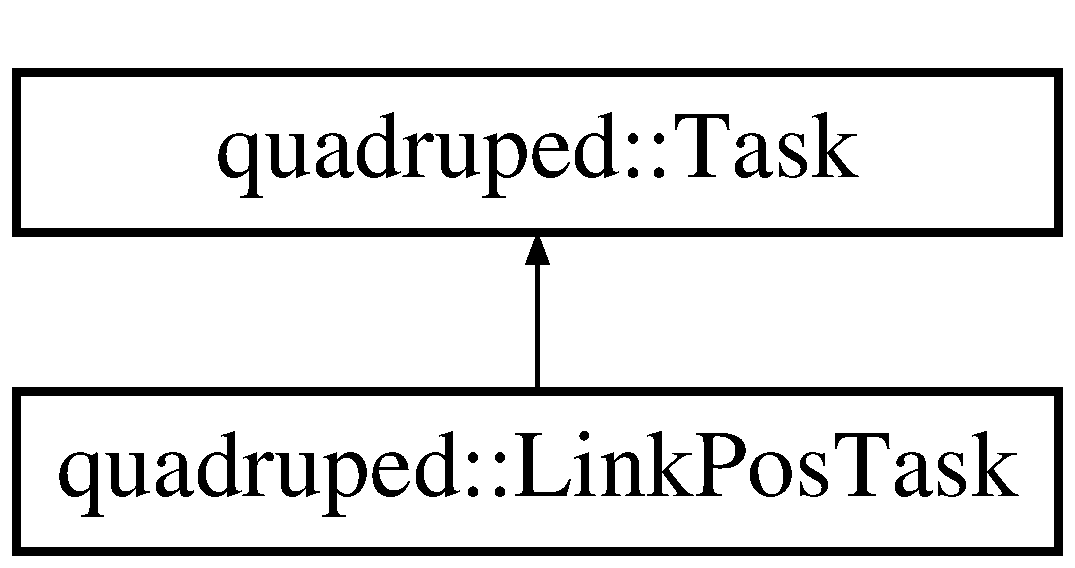
\includegraphics[height=2.000000cm]{classquadruped_1_1LinkPosTask}
\end{center}
\end{figure}
\subsection*{Public 成员函数}
\begin{DoxyCompactItemize}
\item 
\mbox{\Hypertarget{classquadruped_1_1LinkPosTask_abac0cf41a4cf13010f0cea1ca943810b}\label{classquadruped_1_1LinkPosTask_abac0cf41a4cf13010f0cea1ca943810b}} 
{\bfseries Link\+Pos\+Task} (\hyperlink{classquadruped_1_1RobotModel}{Robot\+Model} $\ast$p\+\_\+robot\+Model, const int p\+\_\+link\+Id)
\end{DoxyCompactItemize}
\subsection*{Public 属性}
\begin{DoxyCompactItemize}
\item 
\mbox{\Hypertarget{classquadruped_1_1LinkPosTask_a60e45231e0abc56aefd89ccb795d1f1c}\label{classquadruped_1_1LinkPosTask_a60e45231e0abc56aefd89ccb795d1f1c}} 
\hyperlink{cppTypes_8h_a65c27bf97693676535dd0b30ea0ad399}{Vec3}$<$ double $>$ {\bfseries kp\+\_\+kin}
\item 
\mbox{\Hypertarget{classquadruped_1_1LinkPosTask_a7e662f1f8940c52337886ed33bb179e4}\label{classquadruped_1_1LinkPosTask_a7e662f1f8940c52337886ed33bb179e4}} 
\hyperlink{cppTypes_8h_a65c27bf97693676535dd0b30ea0ad399}{Vec3}$<$ double $>$ {\bfseries kp}
\item 
\mbox{\Hypertarget{classquadruped_1_1LinkPosTask_a4407ff2792b938d8375393cc5812832a}\label{classquadruped_1_1LinkPosTask_a4407ff2792b938d8375393cc5812832a}} 
\hyperlink{cppTypes_8h_a65c27bf97693676535dd0b30ea0ad399}{Vec3}$<$ double $>$ {\bfseries kd}
\item 
\mbox{\Hypertarget{classquadruped_1_1LinkPosTask_ac4ece1b22022feb35b20156363b11fc4}\label{classquadruped_1_1LinkPosTask_ac4ece1b22022feb35b20156363b11fc4}} 
int {\bfseries link\+Id}
\end{DoxyCompactItemize}
\subsection*{Protected 成员函数}
\begin{DoxyCompactItemize}
\item 
\mbox{\Hypertarget{classquadruped_1_1LinkPosTask_a24daaf2d9cfdfb2198f4a7aba29f8efc}\label{classquadruped_1_1LinkPosTask_a24daaf2d9cfdfb2198f4a7aba29f8efc}} 
virtual bool {\bfseries Update\+Command} (const \hyperlink{cppTypes_8h_adad69baca3c77d5f991be5d3c063fea7}{D\+Vec}$<$ double $>$ \&p\+\_\+pos\+\_\+des, const \hyperlink{cppTypes_8h_adad69baca3c77d5f991be5d3c063fea7}{D\+Vec}$<$ double $>$ \&p\+\_\+vel\+\_\+des, const \hyperlink{cppTypes_8h_adad69baca3c77d5f991be5d3c063fea7}{D\+Vec}$<$ double $>$ \&p\+\_\+acc\+\_\+des)
\item 
\mbox{\Hypertarget{classquadruped_1_1LinkPosTask_ab5a6df13f20dc557b91ecaf870e134f6}\label{classquadruped_1_1LinkPosTask_ab5a6df13f20dc557b91ecaf870e134f6}} 
virtual bool {\bfseries Update\+Task\+Jacobian} (void)
\item 
\mbox{\Hypertarget{classquadruped_1_1LinkPosTask_a09dfd84a3acdb8b1d083a7e62b5e562a}\label{classquadruped_1_1LinkPosTask_a09dfd84a3acdb8b1d083a7e62b5e562a}} 
virtual bool {\bfseries Update\+Task\+J\+Dot\+Qdot} (void)
\item 
\mbox{\Hypertarget{classquadruped_1_1LinkPosTask_a6bbd706b0575f0fc586e96ccca4ebbcc}\label{classquadruped_1_1LinkPosTask_a6bbd706b0575f0fc586e96ccca4ebbcc}} 
virtual bool {\bfseries Additional\+Update} (void)
\end{DoxyCompactItemize}
\subsection*{Protected 属性}
\begin{DoxyCompactItemize}
\item 
\mbox{\Hypertarget{classquadruped_1_1LinkPosTask_a69cf63b4e9b9e8c290b0fe56f75a80f5}\label{classquadruped_1_1LinkPosTask_a69cf63b4e9b9e8c290b0fe56f75a80f5}} 
\hyperlink{classquadruped_1_1RobotModel}{Robot\+Model} $\ast$ {\bfseries robot\+Model}
\end{DoxyCompactItemize}


该类的文档由以下文件生成\+:\begin{DoxyCompactItemize}
\item 
controller/wbc/task\+Set/link\+Pos\+Task.\+hpp\item 
controller/wbc/task\+Set/\hyperlink{linkPosTask_8cpp}{link\+Pos\+Task.\+cpp}\end{DoxyCompactItemize}

\hypertarget{classquadruped_1_1LocomotionCtrl}{}\section{quadruped\+:\+:Locomotion\+Ctrl类 参考}
\label{classquadruped_1_1LocomotionCtrl}\index{quadruped\+::\+Locomotion\+Ctrl@{quadruped\+::\+Locomotion\+Ctrl}}


Actiger运动控制类  




{\ttfamily \#include $<$locomotion\+Controller.\+hpp$>$}

\subsection*{Public 成员函数}
\begin{DoxyCompactItemize}
\item 
\mbox{\Hypertarget{classquadruped_1_1LocomotionCtrl_a233d4539571e8970451e1bf800a5eeb8}\label{classquadruped_1_1LocomotionCtrl_a233d4539571e8970451e1bf800a5eeb8}} 
\hyperlink{classquadruped_1_1LocomotionCtrl_a233d4539571e8970451e1bf800a5eeb8}{Locomotion\+Ctrl} (void)
\begin{DoxyCompactList}\small\item\em Locomotion\+Ctrl类的构造函数，完成所有对象成员的内存分配 \end{DoxyCompactList}\item 
\mbox{\Hypertarget{classquadruped_1_1LocomotionCtrl_a94ec7af0dc2d159e91bdc541c00e34fd}\label{classquadruped_1_1LocomotionCtrl_a94ec7af0dc2d159e91bdc541c00e34fd}} 
virtual \hyperlink{classquadruped_1_1LocomotionCtrl_a94ec7af0dc2d159e91bdc541c00e34fd}{$\sim$\+Locomotion\+Ctrl} (void)
\begin{DoxyCompactList}\small\item\em Locomotion\+Ctrl类的析构函数，释放申请的内存 \end{DoxyCompactList}\item 
\mbox{\Hypertarget{classquadruped_1_1LocomotionCtrl_ae1ea49db9859d92fb33a4959dadfeeee}\label{classquadruped_1_1LocomotionCtrl_ae1ea49db9859d92fb33a4959dadfeeee}} 
void \hyperlink{classquadruped_1_1LocomotionCtrl_ae1ea49db9859d92fb33a4959dadfeeee}{Robot\+Control} (void)
\begin{DoxyCompactList}\small\item\em 机器人控制函数 \end{DoxyCompactList}\end{DoxyCompactItemize}
\subsection*{Public 属性}
\begin{DoxyCompactItemize}
\item 
\mbox{\Hypertarget{classquadruped_1_1LocomotionCtrl_af2e5cc2d85c00e73c580aebf5b6db19f}\label{classquadruped_1_1LocomotionCtrl_af2e5cc2d85c00e73c580aebf5b6db19f}} 
\hyperlink{classquadruped_1_1Mpc}{Mpc} $\ast$ \hyperlink{classquadruped_1_1LocomotionCtrl_af2e5cc2d85c00e73c580aebf5b6db19f}{mpc}
\begin{DoxyCompactList}\small\item\em Mpc类的实例化对象，\+Actiger模型预测控制器 \end{DoxyCompactList}\item 
\mbox{\Hypertarget{classquadruped_1_1LocomotionCtrl_afb4fdfa9aeafca4990b964be1760a291}\label{classquadruped_1_1LocomotionCtrl_afb4fdfa9aeafca4990b964be1760a291}} 
\hyperlink{classquadruped_1_1RobotModel}{Robot\+Model} $\ast$ \hyperlink{classquadruped_1_1LocomotionCtrl_afb4fdfa9aeafca4990b964be1760a291}{robot\+Model}
\begin{DoxyCompactList}\small\item\em Robot\+Model类的实例化对象，存储机器人模型信息 \end{DoxyCompactList}\item 
\mbox{\Hypertarget{classquadruped_1_1LocomotionCtrl_a77f83342b1327735db2ce184d032b697}\label{classquadruped_1_1LocomotionCtrl_a77f83342b1327735db2ce184d032b697}} 
\hyperlink{classquadruped_1_1Parameters}{Parameters} $\ast$ \hyperlink{classquadruped_1_1LocomotionCtrl_a77f83342b1327735db2ce184d032b697}{para}
\begin{DoxyCompactList}\small\item\em Parameters类的实例化对象，存储一些被频繁使用的参数 \end{DoxyCompactList}\item 
\mbox{\Hypertarget{classquadruped_1_1LocomotionCtrl_a27b80b6c14c2153e3c3ad367d4411805}\label{classquadruped_1_1LocomotionCtrl_a27b80b6c14c2153e3c3ad367d4411805}} 
\hyperlink{classquadruped_1_1MotionPlan}{Motion\+Plan} $\ast$ \hyperlink{classquadruped_1_1LocomotionCtrl_a27b80b6c14c2153e3c3ad367d4411805}{motion\+Plan}
\begin{DoxyCompactList}\small\item\em Motion\+Plan类的实例化对象，\+Actiger规划器 \end{DoxyCompactList}\item 
\mbox{\Hypertarget{classquadruped_1_1LocomotionCtrl_a46951dff3fd3eb4b0d050bf831b05a4e}\label{classquadruped_1_1LocomotionCtrl_a46951dff3fd3eb4b0d050bf831b05a4e}} 
\hyperlink{classquadruped_1_1LegControl}{Leg\+Control} $\ast$ \hyperlink{classquadruped_1_1LocomotionCtrl_a46951dff3fd3eb4b0d050bf831b05a4e}{leg\+Control}
\begin{DoxyCompactList}\small\item\em Leg\+Control类的实例化对象，\+Actiger腿部控制器 \end{DoxyCompactList}\item 
\mbox{\Hypertarget{classquadruped_1_1LocomotionCtrl_a972cced6a5cac9fbfc8a324cad41c04d}\label{classquadruped_1_1LocomotionCtrl_a972cced6a5cac9fbfc8a324cad41c04d}} 
\hyperlink{cppTypes_8h_a87f228860242acc66da2e58086d18cec}{Vec12}$<$ double $>$ {\bfseries mpc\+\_\+pre\+\_\+force} = \hyperlink{cppTypes_8h_a87f228860242acc66da2e58086d18cec}{Vec12}$<$double$>$\+::Zero()
\item 
\mbox{\Hypertarget{classquadruped_1_1LocomotionCtrl_a8dede580a59c915af67d01f4e82fab42}\label{classquadruped_1_1LocomotionCtrl_a8dede580a59c915af67d01f4e82fab42}} 
\hyperlink{cppTypes_8h_a87f228860242acc66da2e58086d18cec}{Vec12}$<$ double $>$ {\bfseries mpc\+\_\+pre\+\_\+pre\+\_\+force} = \hyperlink{cppTypes_8h_a87f228860242acc66da2e58086d18cec}{Vec12}$<$double$>$\+::Zero()
\end{DoxyCompactItemize}


\subsection{详细描述}
Actiger运动控制类 

该类的文档由以下文件生成\+:\begin{DoxyCompactItemize}
\item 
\hyperlink{locomotionController_8hpp}{locomotion\+Controller.\+hpp}\item 
\hyperlink{locomotionController_8cpp}{locomotion\+Controller.\+cpp}\end{DoxyCompactItemize}

\hypertarget{classquadruped_1_1Module}{}\section{quadruped\+:\+:Module类 参考}
\label{classquadruped_1_1Module}\index{quadruped\+::\+Module@{quadruped\+::\+Module}}
\subsection*{Public 成员函数}
\begin{DoxyCompactItemize}
\item 
\mbox{\Hypertarget{classquadruped_1_1Module_a35b9160967ca7f10f66054d09f6fad02}\label{classquadruped_1_1Module_a35b9160967ca7f10f66054d09f6fad02}} 
{\bfseries Module} (\hyperlink{classquadruped_1_1RobotModel}{Robot\+Model} $\ast$p\+\_\+robot\+Model, \hyperlink{classquadruped_1_1Parameters}{Parameters} $\ast$p\+\_\+para, \hyperlink{classquadruped_1_1LegControl}{Leg\+Control} $\ast$p\+\_\+leg\+Control)
\item 
\mbox{\Hypertarget{classquadruped_1_1Module_a3bc90b0998251e6abaaefee7a08c11de}\label{classquadruped_1_1Module_a3bc90b0998251e6abaaefee7a08c11de}} 
void {\bfseries Reset\+Leg} (void)
\item 
\mbox{\Hypertarget{classquadruped_1_1Module_acb56e73f76d0dc28443baad534e70853}\label{classquadruped_1_1Module_acb56e73f76d0dc28443baad534e70853}} 
void {\bfseries Swing\+Test} (\hyperlink{cppTypes_8h_a65c27bf97693676535dd0b30ea0ad399}{Vec3}$<$ double $>$ p\+\_\+pos\+\_\+des, \hyperlink{cppTypes_8h_a65c27bf97693676535dd0b30ea0ad399}{Vec3}$<$ double $>$ p\+\_\+vel\+\_\+des)
\item 
\mbox{\Hypertarget{classquadruped_1_1Module_a3e1100bd58a23d0a921d94bad2737242}\label{classquadruped_1_1Module_a3e1100bd58a23d0a921d94bad2737242}} 
void {\bfseries Torque\+Limit} (\hyperlink{cppTypes_8h_a65c27bf97693676535dd0b30ea0ad399}{Vec3}$<$ double $>$ \&p\+\_\+torque)
\end{DoxyCompactItemize}
\subsection*{Public 属性}
\begin{DoxyCompactItemize}
\item 
\mbox{\Hypertarget{classquadruped_1_1Module_ad305afcca90df7b15669fe23d133d6ec}\label{classquadruped_1_1Module_ad305afcca90df7b15669fe23d133d6ec}} 
\hyperlink{classquadruped_1_1LegControl}{Leg\+Control} $\ast$ {\bfseries leg\+Control}
\item 
\mbox{\Hypertarget{classquadruped_1_1Module_a170dbfbd831d2447eeefa7cce88fd9dc}\label{classquadruped_1_1Module_a170dbfbd831d2447eeefa7cce88fd9dc}} 
\hyperlink{classquadruped_1_1RobotModel}{Robot\+Model} $\ast$ {\bfseries robot\+Model}
\item 
\mbox{\Hypertarget{classquadruped_1_1Module_ad4cbc63075ea99e920feab5c1c2d103d}\label{classquadruped_1_1Module_ad4cbc63075ea99e920feab5c1c2d103d}} 
\hyperlink{classquadruped_1_1Parameters}{Parameters} $\ast$ {\bfseries para}
\end{DoxyCompactItemize}


该类的文档由以下文件生成\+:\begin{DoxyCompactItemize}
\item 
controller/module/module.\+hpp\item 
controller/module/module.\+cpp\end{DoxyCompactItemize}

\hypertarget{classquadruped_1_1MotionPlan}{}\section{quadruped\+:\+:Motion\+Plan类 参考}
\label{classquadruped_1_1MotionPlan}\index{quadruped\+::\+Motion\+Plan@{quadruped\+::\+Motion\+Plan}}


Actiger规划器  




{\ttfamily \#include $<$motion\+Plan.\+hpp$>$}

\subsection*{Public 成员函数}
\begin{DoxyCompactItemize}
\item 
\hyperlink{classquadruped_1_1MotionPlan_af79f137bc037fa02681bded5c26b3a98}{Motion\+Plan} (\hyperlink{classquadruped_1_1RobotModel}{Robot\+Model} $\ast$p\+\_\+robot\+Model, \hyperlink{classquadruped_1_1Parameters}{Parameters} $\ast$p\+\_\+para)
\begin{DoxyCompactList}\small\item\em Motion\+Plan类的构造函数，完成所有对象成员的内存分配及数据成员的初值装载 \end{DoxyCompactList}\item 
\mbox{\Hypertarget{classquadruped_1_1MotionPlan_a0b9fd05864416d513ef8fc144b2ce4c5}\label{classquadruped_1_1MotionPlan_a0b9fd05864416d513ef8fc144b2ce4c5}} 
virtual \hyperlink{classquadruped_1_1MotionPlan_a0b9fd05864416d513ef8fc144b2ce4c5}{$\sim$\+Motion\+Plan} (void)
\begin{DoxyCompactList}\small\item\em Motion\+Plan类的析构函数，释放申请的内存 \end{DoxyCompactList}\item 
\mbox{\Hypertarget{classquadruped_1_1MotionPlan_ab8e8aa634d2bc8cc8d10ae16d8e4b928}\label{classquadruped_1_1MotionPlan_ab8e8aa634d2bc8cc8d10ae16d8e4b928}} 
void \hyperlink{classquadruped_1_1MotionPlan_ab8e8aa634d2bc8cc8d10ae16d8e4b928}{Robot\+Motion\+Plan} (void)
\begin{DoxyCompactList}\small\item\em Actiger核心规划函数 \end{DoxyCompactList}\item 
\mbox{\Hypertarget{classquadruped_1_1MotionPlan_a4aab89067581b6c44636eed8e71fb8c2}\label{classquadruped_1_1MotionPlan_a4aab89067581b6c44636eed8e71fb8c2}} 
void \hyperlink{classquadruped_1_1MotionPlan_a4aab89067581b6c44636eed8e71fb8c2}{Set\+Cmd} (void)
\begin{DoxyCompactList}\small\item\em 将\+Actiger规划器求得的期望序列写入队列 \end{DoxyCompactList}\item 
\mbox{\Hypertarget{classquadruped_1_1MotionPlan_ac9ab5a55e108b3ca024a61de0402328a}\label{classquadruped_1_1MotionPlan_ac9ab5a55e108b3ca024a61de0402328a}} 
void \hyperlink{classquadruped_1_1MotionPlan_ac9ab5a55e108b3ca024a61de0402328a}{Updata\+Info} (void)
\begin{DoxyCompactList}\small\item\em 更新\+Actiger规划信息 \end{DoxyCompactList}\item 
void \hyperlink{classquadruped_1_1MotionPlan_a46f0f22ad97c07959a86eb055778455e}{Set\+Terrain} (uint8\+\_\+t p\+\_\+terrain\+Type)
\begin{DoxyCompactList}\small\item\em 根据形参p\+\_\+terrain\+Type设置当前地形 \end{DoxyCompactList}\item 
\mbox{\Hypertarget{classquadruped_1_1MotionPlan_a67cb0a9de47d8692a7f771f53ded75d7}\label{classquadruped_1_1MotionPlan_a67cb0a9de47d8692a7f771f53ded75d7}} 
void \hyperlink{classquadruped_1_1MotionPlan_a67cb0a9de47d8692a7f771f53ded75d7}{Start} (void)
\begin{DoxyCompactList}\small\item\em Actiger规划标志位处理函数 \end{DoxyCompactList}\item 
\mbox{\Hypertarget{classquadruped_1_1MotionPlan_ace34ba5ac538bf888557f3ce018b13aa}\label{classquadruped_1_1MotionPlan_ace34ba5ac538bf888557f3ce018b13aa}} 
void \hyperlink{classquadruped_1_1MotionPlan_ace34ba5ac538bf888557f3ce018b13aa}{Display\+Body\+Traj} (void)
\begin{DoxyCompactList}\small\item\em 机体轨迹可视化 \end{DoxyCompactList}\item 
\mbox{\Hypertarget{classquadruped_1_1MotionPlan_afdaeeb4026e7d7b1addf141ff6cc3eb3}\label{classquadruped_1_1MotionPlan_afdaeeb4026e7d7b1addf141ff6cc3eb3}} 
void \hyperlink{classquadruped_1_1MotionPlan_afdaeeb4026e7d7b1addf141ff6cc3eb3}{Display\+L\+F\+Traj} (void)
\begin{DoxyCompactList}\small\item\em 左前腿足端轨迹可视化 \end{DoxyCompactList}\item 
\mbox{\Hypertarget{classquadruped_1_1MotionPlan_a7d7a02f70830250460259f8d4c19f3d4}\label{classquadruped_1_1MotionPlan_a7d7a02f70830250460259f8d4c19f3d4}} 
void \hyperlink{classquadruped_1_1MotionPlan_a7d7a02f70830250460259f8d4c19f3d4}{Display\+L\+R\+Traj} (void)
\begin{DoxyCompactList}\small\item\em 左后腿足端轨迹可视化 \end{DoxyCompactList}\item 
\mbox{\Hypertarget{classquadruped_1_1MotionPlan_aac565c83a33285acaef89043f1c4ff84}\label{classquadruped_1_1MotionPlan_aac565c83a33285acaef89043f1c4ff84}} 
void \hyperlink{classquadruped_1_1MotionPlan_aac565c83a33285acaef89043f1c4ff84}{Display\+R\+F\+Traj} (void)
\begin{DoxyCompactList}\small\item\em 右前腿足端轨迹可视化 \end{DoxyCompactList}\item 
\mbox{\Hypertarget{classquadruped_1_1MotionPlan_a1744cc35523b9978cab9077ab1f7fa7f}\label{classquadruped_1_1MotionPlan_a1744cc35523b9978cab9077ab1f7fa7f}} 
void \hyperlink{classquadruped_1_1MotionPlan_a1744cc35523b9978cab9077ab1f7fa7f}{Display\+R\+R\+Traj} (void)
\begin{DoxyCompactList}\small\item\em 右后腿足端轨迹可视化 \end{DoxyCompactList}\end{DoxyCompactItemize}
\subsection*{Public 属性}
\begin{DoxyCompactItemize}
\item 
\mbox{\Hypertarget{classquadruped_1_1MotionPlan_a4d6a1024fc5a2612dca34af18fe5998d}\label{classquadruped_1_1MotionPlan_a4d6a1024fc5a2612dca34af18fe5998d}} 
double \hyperlink{classquadruped_1_1MotionPlan_a4d6a1024fc5a2612dca34af18fe5998d}{Ts}
\begin{DoxyCompactList}\small\item\em 一个完整步态周期中的支撑相所占时间 \end{DoxyCompactList}\item 
\mbox{\Hypertarget{classquadruped_1_1MotionPlan_a7d5ada02315ce7346bd441c92c5156a5}\label{classquadruped_1_1MotionPlan_a7d5ada02315ce7346bd441c92c5156a5}} 
int \hyperlink{classquadruped_1_1MotionPlan_a7d5ada02315ce7346bd441c92c5156a5}{grid}
\begin{DoxyCompactList}\small\item\em 把一个\+Ts时间跨度分割成grid个\+M\+P\+C周期 \end{DoxyCompactList}\item 
\mbox{\Hypertarget{classquadruped_1_1MotionPlan_af5ed3b39ee344757263733bed5731f7e}\label{classquadruped_1_1MotionPlan_af5ed3b39ee344757263733bed5731f7e}} 
bool \hyperlink{classquadruped_1_1MotionPlan_af5ed3b39ee344757263733bed5731f7e}{is\+\_\+lf\+\_\+rr\+\_\+stand}
\begin{DoxyCompactList}\small\item\em 表示支撑腿组合的标志位 \end{DoxyCompactList}\item 
\mbox{\Hypertarget{classquadruped_1_1MotionPlan_ad994c500c74ec400b375115edda79ce5}\label{classquadruped_1_1MotionPlan_ad994c500c74ec400b375115edda79ce5}} 
bool \hyperlink{classquadruped_1_1MotionPlan_ad994c500c74ec400b375115edda79ce5}{plan\+Flag} = 0
\begin{DoxyCompactList}\small\item\em 判断是否进行一次规划的标志位 \end{DoxyCompactList}\item 
\mbox{\Hypertarget{classquadruped_1_1MotionPlan_ad0e16c69f420367d4d05140b15db2342}\label{classquadruped_1_1MotionPlan_ad0e16c69f420367d4d05140b15db2342}} 
uint8\+\_\+t \hyperlink{classquadruped_1_1MotionPlan_ad0e16c69f420367d4d05140b15db2342}{gait\+Now}
\begin{DoxyCompactList}\small\item\em Actiger当前步态 \end{DoxyCompactList}\item 
\mbox{\Hypertarget{classquadruped_1_1MotionPlan_ac5ae4970fcfccaa355ee23d0638c3914}\label{classquadruped_1_1MotionPlan_ac5ae4970fcfccaa355ee23d0638c3914}} 
\hyperlink{classquadruped_1_1Queue}{Queue} $\ast$ \hyperlink{classquadruped_1_1MotionPlan_ac5ae4970fcfccaa355ee23d0638c3914}{p\+Body\+\_\+euler\+\_\+des}
\begin{DoxyCompactList}\small\item\em 期望的机体欧拉角队列 \end{DoxyCompactList}\item 
\mbox{\Hypertarget{classquadruped_1_1MotionPlan_ae04b0144696e2aeefc63839c31405ebc}\label{classquadruped_1_1MotionPlan_ae04b0144696e2aeefc63839c31405ebc}} 
\hyperlink{classquadruped_1_1Queue}{Queue} $\ast$ \hyperlink{classquadruped_1_1MotionPlan_ae04b0144696e2aeefc63839c31405ebc}{v\+Body\+\_\+euler\+\_\+des}
\begin{DoxyCompactList}\small\item\em 期望的机体欧拉角速度队列 \end{DoxyCompactList}\item 
\mbox{\Hypertarget{classquadruped_1_1MotionPlan_a069f14762dbb266d0aadfa10ae31de07}\label{classquadruped_1_1MotionPlan_a069f14762dbb266d0aadfa10ae31de07}} 
\hyperlink{classquadruped_1_1Queue}{Queue} $\ast$ \hyperlink{classquadruped_1_1MotionPlan_a069f14762dbb266d0aadfa10ae31de07}{p\+Body\+\_\+des}
\begin{DoxyCompactList}\small\item\em 期望的机体位置队列 \end{DoxyCompactList}\item 
\mbox{\Hypertarget{classquadruped_1_1MotionPlan_a3fa85fe450feebd7e92d2ac44120716d}\label{classquadruped_1_1MotionPlan_a3fa85fe450feebd7e92d2ac44120716d}} 
\hyperlink{classquadruped_1_1Queue}{Queue} $\ast$ \hyperlink{classquadruped_1_1MotionPlan_a3fa85fe450feebd7e92d2ac44120716d}{v\+Body\+\_\+des}
\begin{DoxyCompactList}\small\item\em 期望的机体速度队列 \end{DoxyCompactList}\item 
\mbox{\Hypertarget{classquadruped_1_1MotionPlan_a76ba519765eb863905ba1010e69bbb01}\label{classquadruped_1_1MotionPlan_a76ba519765eb863905ba1010e69bbb01}} 
\hyperlink{classquadruped_1_1Queue}{Queue} $\ast$ \hyperlink{classquadruped_1_1MotionPlan_a76ba519765eb863905ba1010e69bbb01}{a\+Body\+\_\+des}
\begin{DoxyCompactList}\small\item\em 期望的机体加速度队列 \end{DoxyCompactList}\item 
\mbox{\Hypertarget{classquadruped_1_1MotionPlan_a9de493b6d7cfeb7820cfbcbfc75a7664}\label{classquadruped_1_1MotionPlan_a9de493b6d7cfeb7820cfbcbfc75a7664}} 
\hyperlink{classquadruped_1_1Gamepad}{Gamepad} $\ast$ \hyperlink{classquadruped_1_1MotionPlan_a9de493b6d7cfeb7820cfbcbfc75a7664}{gamepad}
\begin{DoxyCompactList}\small\item\em Gamepad类的实例化对象，\+Actiger遥控器 \end{DoxyCompactList}\item 
\mbox{\Hypertarget{classquadruped_1_1MotionPlan_a55aa8bfff1dc59cf60459d3e110218c1}\label{classquadruped_1_1MotionPlan_a55aa8bfff1dc59cf60459d3e110218c1}} 
\hyperlink{classquadruped_1_1StateMachine}{State\+Machine} $\ast$ \hyperlink{classquadruped_1_1MotionPlan_a55aa8bfff1dc59cf60459d3e110218c1}{state\+Machine}
\begin{DoxyCompactList}\small\item\em State\+Machine类的实例化对象，\+Actiger状态机 \end{DoxyCompactList}\item 
\mbox{\Hypertarget{classquadruped_1_1MotionPlan_aa1bc9af0d38eb216f38f5a522e299b65}\label{classquadruped_1_1MotionPlan_aa1bc9af0d38eb216f38f5a522e299b65}} 
\hyperlink{classquadruped_1_1RobotModel}{Robot\+Model} $\ast$ \hyperlink{classquadruped_1_1MotionPlan_aa1bc9af0d38eb216f38f5a522e299b65}{robot\+Model}
\begin{DoxyCompactList}\small\item\em Robot\+Model类的实例化对象，存储机器人模型信息 \end{DoxyCompactList}\item 
\mbox{\Hypertarget{classquadruped_1_1MotionPlan_a89e7b9a6130d9fc312a407c97017c56f}\label{classquadruped_1_1MotionPlan_a89e7b9a6130d9fc312a407c97017c56f}} 
\hyperlink{classquadruped_1_1Parameters}{Parameters} $\ast$ \hyperlink{classquadruped_1_1MotionPlan_a89e7b9a6130d9fc312a407c97017c56f}{para}
\begin{DoxyCompactList}\small\item\em Parameters类的实例化对象，存储一些被频繁使用的参数 \end{DoxyCompactList}\item 
\mbox{\Hypertarget{classquadruped_1_1MotionPlan_a7ea20a7cfb4c72e7f37be61676840705}\label{classquadruped_1_1MotionPlan_a7ea20a7cfb4c72e7f37be61676840705}} 
\hyperlink{classquadruped_1_1Foothold}{Foothold} $\ast$ \hyperlink{classquadruped_1_1MotionPlan_a7ea20a7cfb4c72e7f37be61676840705}{foothold}
\begin{DoxyCompactList}\small\item\em Foothold类的实例化对象，\+Actiger落足点规划器 \end{DoxyCompactList}\item 
\mbox{\Hypertarget{classquadruped_1_1MotionPlan_a4aefeb143bd9bb2e0e0460b90dc3b43f}\label{classquadruped_1_1MotionPlan_a4aefeb143bd9bb2e0e0460b90dc3b43f}} 
\hyperlink{classquadruped_1_1BodyTrajectory}{Body\+Trajectory} $\ast$ \hyperlink{classquadruped_1_1MotionPlan_a4aefeb143bd9bb2e0e0460b90dc3b43f}{body\+Trajectory}
\begin{DoxyCompactList}\small\item\em Body\+Trajectory类的实例化对象，\+Actiger机体轨迹规划器 \end{DoxyCompactList}\item 
\mbox{\Hypertarget{classquadruped_1_1MotionPlan_ab2272c920c3b4311023fb4c1103436ad}\label{classquadruped_1_1MotionPlan_ab2272c920c3b4311023fb4c1103436ad}} 
\hyperlink{classquadruped_1_1EndfootTrajectory}{Endfoot\+Trajectory} $\ast$ \hyperlink{classquadruped_1_1MotionPlan_ab2272c920c3b4311023fb4c1103436ad}{endfoot\+Trajectory}
\begin{DoxyCompactList}\small\item\em Endfoot\+Trajectory类的实例化对象，\+Actiger摆动腿足端轨迹规划器 \end{DoxyCompactList}\item 
\mbox{\Hypertarget{classquadruped_1_1MotionPlan_a58280188cf51d2e936d6dc4aa7520859}\label{classquadruped_1_1MotionPlan_a58280188cf51d2e936d6dc4aa7520859}} 
std\+::vector$<$ \hyperlink{classquadruped_1_1LegPlan}{Leg\+Plan} $\ast$ $>$ \hyperlink{classquadruped_1_1MotionPlan_a58280188cf51d2e936d6dc4aa7520859}{leg\+Plan}
\begin{DoxyCompactList}\small\item\em Leg\+Plan类的实例化对象向量，存储\+Actiger腿部的规划结果 \end{DoxyCompactList}\item 
\mbox{\Hypertarget{classquadruped_1_1MotionPlan_a8efab4af4a0c1264204a0d12baeb5494}\label{classquadruped_1_1MotionPlan_a8efab4af4a0c1264204a0d12baeb5494}} 
\hyperlink{classquadruped_1_1LegPlan}{Leg\+Plan} $\ast$ \hyperlink{classquadruped_1_1MotionPlan_a8efab4af4a0c1264204a0d12baeb5494}{lf}
\begin{DoxyCompactList}\small\item\em Leg\+Plan类的实例化对象，存储\+Actiger左前腿的规划结果 \end{DoxyCompactList}\item 
\mbox{\Hypertarget{classquadruped_1_1MotionPlan_a05dd0137376852bb6feee04f6193c5f6}\label{classquadruped_1_1MotionPlan_a05dd0137376852bb6feee04f6193c5f6}} 
\hyperlink{classquadruped_1_1LegPlan}{Leg\+Plan} $\ast$ \hyperlink{classquadruped_1_1MotionPlan_a05dd0137376852bb6feee04f6193c5f6}{lr}
\begin{DoxyCompactList}\small\item\em Leg\+Plan类的实例化对象，存储\+Actiger左后腿的规划结果 \end{DoxyCompactList}\item 
\mbox{\Hypertarget{classquadruped_1_1MotionPlan_a0b4b74a58595e74bd8a1407ef8e82edf}\label{classquadruped_1_1MotionPlan_a0b4b74a58595e74bd8a1407ef8e82edf}} 
\hyperlink{classquadruped_1_1LegPlan}{Leg\+Plan} $\ast$ \hyperlink{classquadruped_1_1MotionPlan_a0b4b74a58595e74bd8a1407ef8e82edf}{rf}
\begin{DoxyCompactList}\small\item\em Leg\+Plan类的实例化对象，存储\+Actiger右前腿的规划结果 \end{DoxyCompactList}\item 
\mbox{\Hypertarget{classquadruped_1_1MotionPlan_aa634067d342c0ec0bdf71c5333f84d11}\label{classquadruped_1_1MotionPlan_aa634067d342c0ec0bdf71c5333f84d11}} 
\hyperlink{classquadruped_1_1LegPlan}{Leg\+Plan} $\ast$ \hyperlink{classquadruped_1_1MotionPlan_aa634067d342c0ec0bdf71c5333f84d11}{rr}
\begin{DoxyCompactList}\small\item\em Leg\+Plan类的实例化对象，存储\+Actiger右后腿的规划结果 \end{DoxyCompactList}\item 
\mbox{\Hypertarget{classquadruped_1_1MotionPlan_ac27061731dfc05e5f2ab3b8b29404a35}\label{classquadruped_1_1MotionPlan_ac27061731dfc05e5f2ab3b8b29404a35}} 
\hyperlink{classquadruped_1_1Terrain}{Terrain} $\ast$ \hyperlink{classquadruped_1_1MotionPlan_ac27061731dfc05e5f2ab3b8b29404a35}{terrain\+\_\+now}
\begin{DoxyCompactList}\small\item\em Terrain类的实例化对象，表示当前的地形 \end{DoxyCompactList}\item 
\mbox{\Hypertarget{classquadruped_1_1MotionPlan_ab985d804440413e397e2e166fd1bb190}\label{classquadruped_1_1MotionPlan_ab985d804440413e397e2e166fd1bb190}} 
\hyperlink{classquadruped_1_1FlatGround}{Flat\+Ground} $\ast$ \hyperlink{classquadruped_1_1MotionPlan_ab985d804440413e397e2e166fd1bb190}{flat\+Ground}
\begin{DoxyCompactList}\small\item\em Flat\+Ground类的实例化对象，表示平地 \end{DoxyCompactList}\item 
\mbox{\Hypertarget{classquadruped_1_1MotionPlan_a12274c307b46b1b6e04385095427e46c}\label{classquadruped_1_1MotionPlan_a12274c307b46b1b6e04385095427e46c}} 
\hyperlink{classquadruped_1_1Slope}{Slope} $\ast$ \hyperlink{classquadruped_1_1MotionPlan_a12274c307b46b1b6e04385095427e46c}{slope}
\begin{DoxyCompactList}\small\item\em Slope类的实例化对象，表示坡面 \end{DoxyCompactList}\item 
\mbox{\Hypertarget{classquadruped_1_1MotionPlan_aa8bbab60ae1b26742398d8e7dadd81ff}\label{classquadruped_1_1MotionPlan_aa8bbab60ae1b26742398d8e7dadd81ff}} 
\hyperlink{classquadruped_1_1Stage}{Stage} $\ast$ \hyperlink{classquadruped_1_1MotionPlan_aa8bbab60ae1b26742398d8e7dadd81ff}{stage}
\begin{DoxyCompactList}\small\item\em Stage类的实例化对象，表示平台 \end{DoxyCompactList}\item 
\mbox{\Hypertarget{classquadruped_1_1MotionPlan_a5273d32d1cd281eff55aa996c461d800}\label{classquadruped_1_1MotionPlan_a5273d32d1cd281eff55aa996c461d800}} 
\hyperlink{classquadruped_1_1Sill}{Sill} $\ast$ \hyperlink{classquadruped_1_1MotionPlan_a5273d32d1cd281eff55aa996c461d800}{sill}
\begin{DoxyCompactList}\small\item\em Sill类的实例化对象，表示门槛 \end{DoxyCompactList}\item 
\mbox{\Hypertarget{classquadruped_1_1MotionPlan_a4ac430012abb35e9051bead7b7c4b864}\label{classquadruped_1_1MotionPlan_a4ac430012abb35e9051bead7b7c4b864}} 
\hyperlink{classquadruped_1_1Stairs}{Stairs} $\ast$ \hyperlink{classquadruped_1_1MotionPlan_a4ac430012abb35e9051bead7b7c4b864}{stairs}
\begin{DoxyCompactList}\small\item\em Stairs类的实例化对象，表示阶梯 \end{DoxyCompactList}\item 
\mbox{\Hypertarget{classquadruped_1_1MotionPlan_ac870f7f2c75f6cdf4a367303565e793a}\label{classquadruped_1_1MotionPlan_ac870f7f2c75f6cdf4a367303565e793a}} 
\hyperlink{classquadruped_1_1Calandria}{Calandria} $\ast$ \hyperlink{classquadruped_1_1MotionPlan_ac870f7f2c75f6cdf4a367303565e793a}{calandria}
\begin{DoxyCompactList}\small\item\em Calandria类的实例化对象，表示排管 \end{DoxyCompactList}\item 
\mbox{\Hypertarget{classquadruped_1_1MotionPlan_a0e6e197d5f0601600c4a05c36168cbcb}\label{classquadruped_1_1MotionPlan_a0e6e197d5f0601600c4a05c36168cbcb}} 
\hyperlink{classquadruped_1_1Hurdles}{Hurdles} $\ast$ \hyperlink{classquadruped_1_1MotionPlan_a0e6e197d5f0601600c4a05c36168cbcb}{hurdles}
\begin{DoxyCompactList}\small\item\em Hurdles类的实例化对象，表示横杆 \end{DoxyCompactList}\item 
\mbox{\Hypertarget{classquadruped_1_1MotionPlan_ad5b9d0be05dcdf97ee22816146112e88}\label{classquadruped_1_1MotionPlan_ad5b9d0be05dcdf97ee22816146112e88}} 
\hyperlink{classquadruped_1_1Ballpool}{Ballpool} $\ast$ \hyperlink{classquadruped_1_1MotionPlan_ad5b9d0be05dcdf97ee22816146112e88}{ballpool}
\begin{DoxyCompactList}\small\item\em Ballpool类的实例化对象，表示球池 \end{DoxyCompactList}\item 
\mbox{\Hypertarget{classquadruped_1_1MotionPlan_ad297ad596a1a813b45c4e28f11304a32}\label{classquadruped_1_1MotionPlan_ad297ad596a1a813b45c4e28f11304a32}} 
\hyperlink{classquadruped_1_1Seesaw}{Seesaw} $\ast$ \hyperlink{classquadruped_1_1MotionPlan_ad297ad596a1a813b45c4e28f11304a32}{seesaw}
\begin{DoxyCompactList}\small\item\em Seesaw类的实例化对象，表示跷跷板 \end{DoxyCompactList}\item 
\mbox{\Hypertarget{classquadruped_1_1MotionPlan_acbac0999d3d2cb246734b0eba01a01b9}\label{classquadruped_1_1MotionPlan_acbac0999d3d2cb246734b0eba01a01b9}} 
\hyperlink{classquadruped_1_1Bridge}{Bridge} $\ast$ \hyperlink{classquadruped_1_1MotionPlan_acbac0999d3d2cb246734b0eba01a01b9}{bridge}
\begin{DoxyCompactList}\small\item\em Bridge类的实例化对象，表示双木桥 \end{DoxyCompactList}\end{DoxyCompactItemize}


\subsection{详细描述}
Actiger规划器 

\subsection{构造及析构函数说明}
\mbox{\Hypertarget{classquadruped_1_1MotionPlan_af79f137bc037fa02681bded5c26b3a98}\label{classquadruped_1_1MotionPlan_af79f137bc037fa02681bded5c26b3a98}} 
\index{quadruped\+::\+Motion\+Plan@{quadruped\+::\+Motion\+Plan}!Motion\+Plan@{Motion\+Plan}}
\index{Motion\+Plan@{Motion\+Plan}!quadruped\+::\+Motion\+Plan@{quadruped\+::\+Motion\+Plan}}
\subsubsection{\texorpdfstring{Motion\+Plan()}{MotionPlan()}}
{\footnotesize\ttfamily Motion\+Plan\+::\+Motion\+Plan (\begin{DoxyParamCaption}\item[{\hyperlink{classquadruped_1_1RobotModel}{Robot\+Model} $\ast$}]{p\+\_\+robot\+Model,  }\item[{\hyperlink{classquadruped_1_1Parameters}{Parameters} $\ast$}]{p\+\_\+para }\end{DoxyParamCaption})\hspace{0.3cm}{\ttfamily [explicit]}}



Motion\+Plan类的构造函数，完成所有对象成员的内存分配及数据成员的初值装载 


\begin{DoxyParams}{参数}
{\em p\+\_\+robot\+Model} & Robot\+Model类的实例化对象，存储机器人模型信息，用来初始化对象成员robot\+Model \\
\hline
{\em p\+\_\+para} & Parameters类的实例化对象，存储一些被频繁使用的参数，用来初始化对象成员para \\
\hline
\end{DoxyParams}


参考 a\+Body\+\_\+des, ballpool, body\+Trajectory, bridge, calandria, endfoot\+Trajectory, flat\+Ground, foothold, gait\+Now, gamepad, grid, hurdles, I\+N\+I\+T\+\_\+\+H\+E\+I\+G\+HT, is\+\_\+lf\+\_\+rr\+\_\+stand, leg\+Plan, lf, lr, p\+Body\+\_\+des, p\+Body\+\_\+euler\+\_\+des, plan\+Flag, rf, rr, seesaw, sill, slope, stage, stairs, state\+Machine, terrain\+\_\+now, Ts, v\+Body\+\_\+des , 以及 v\+Body\+\_\+euler\+\_\+des.



\subsection{成员函数说明}
\mbox{\Hypertarget{classquadruped_1_1MotionPlan_a46f0f22ad97c07959a86eb055778455e}\label{classquadruped_1_1MotionPlan_a46f0f22ad97c07959a86eb055778455e}} 
\index{quadruped\+::\+Motion\+Plan@{quadruped\+::\+Motion\+Plan}!Set\+Terrain@{Set\+Terrain}}
\index{Set\+Terrain@{Set\+Terrain}!quadruped\+::\+Motion\+Plan@{quadruped\+::\+Motion\+Plan}}
\subsubsection{\texorpdfstring{Set\+Terrain()}{SetTerrain()}}
{\footnotesize\ttfamily void Motion\+Plan\+::\+Set\+Terrain (\begin{DoxyParamCaption}\item[{uint8\+\_\+t}]{p\+\_\+terrain\+Type }\end{DoxyParamCaption})}



根据形参p\+\_\+terrain\+Type设置当前地形 


\begin{DoxyParams}{参数}
{\em p\+\_\+terrain\+Type} & 当前地形，配合感知得到 \\
\hline
\end{DoxyParams}


参考 B\+A\+L\+L\+\_\+\+P\+O\+OL, ballpool, B\+R\+I\+D\+GE, bridge, C\+A\+L\+A\+N\+D\+R\+IA, calandria, endfoot\+Trajectory, F\+L\+AT, flat\+Ground, foothold, H\+U\+R\+D\+L\+ES, hurdles, S\+E\+E\+S\+AW, seesaw, S\+I\+LL, sill, S\+L\+O\+PE, slope, S\+T\+A\+GE, stage, S\+T\+A\+I\+RS, stairs , 以及 terrain\+\_\+now.



参考自 Start().



该类的文档由以下文件生成\+:\begin{DoxyCompactItemize}
\item 
controller/motion\+Plan/\hyperlink{motionPlan_8hpp}{motion\+Plan.\+hpp}\item 
controller/motion\+Plan/\hyperlink{motionPlan_8cpp}{motion\+Plan.\+cpp}\end{DoxyCompactItemize}

\hypertarget{classquadruped_1_1Mpc}{}\section{quadruped\+:\+:Mpc类 参考}
\label{classquadruped_1_1Mpc}\index{quadruped\+::\+Mpc@{quadruped\+::\+Mpc}}


Actiger模型预测控制器  




{\ttfamily \#include $<$mpc.\+hpp$>$}

\subsection*{Public 成员函数}
\begin{DoxyCompactItemize}
\item 
\hyperlink{classquadruped_1_1Mpc_a4bc02766e7c00d69044af00b9c451802}{Mpc} (\hyperlink{classquadruped_1_1RobotModel}{Robot\+Model} $\ast$p\+\_\+robot\+Model, \hyperlink{classquadruped_1_1MotionPlan}{Motion\+Plan} $\ast$p\+\_\+ref, \hyperlink{classquadruped_1_1Parameters}{Parameters} $\ast$p\+\_\+para)
\begin{DoxyCompactList}\small\item\em Actiger模型预测控制器的构造函数，完成对象成员以及部分数据成员的初始化 \end{DoxyCompactList}\item 
\mbox{\Hypertarget{classquadruped_1_1Mpc_a54e96389912459abc9b7ec45741c9ce9}\label{classquadruped_1_1Mpc_a54e96389912459abc9b7ec45741c9ce9}} 
virtual \hyperlink{classquadruped_1_1Mpc_a54e96389912459abc9b7ec45741c9ce9}{$\sim$\+Mpc} ()
\begin{DoxyCompactList}\small\item\em Actiger模型预测控制器的析构函数 \end{DoxyCompactList}\item 
\mbox{\Hypertarget{classquadruped_1_1Mpc_a3f15737db0a0c201de83d5733d1f20f3}\label{classquadruped_1_1Mpc_a3f15737db0a0c201de83d5733d1f20f3}} 
void \hyperlink{classquadruped_1_1Mpc_a3f15737db0a0c201de83d5733d1f20f3}{Get\+React\+Force} (void)
\begin{DoxyCompactList}\small\item\em 构建模型预测控制器，求解二次问题，得到足端力等成员函数的封装 \end{DoxyCompactList}\end{DoxyCompactItemize}


\subsection{详细描述}
Actiger模型预测控制器 

\subsection{构造及析构函数说明}
\mbox{\Hypertarget{classquadruped_1_1Mpc_a4bc02766e7c00d69044af00b9c451802}\label{classquadruped_1_1Mpc_a4bc02766e7c00d69044af00b9c451802}} 
\index{quadruped\+::\+Mpc@{quadruped\+::\+Mpc}!Mpc@{Mpc}}
\index{Mpc@{Mpc}!quadruped\+::\+Mpc@{quadruped\+::\+Mpc}}
\subsubsection{\texorpdfstring{Mpc()}{Mpc()}}
{\footnotesize\ttfamily Mpc\+::\+Mpc (\begin{DoxyParamCaption}\item[{\hyperlink{classquadruped_1_1RobotModel}{Robot\+Model} $\ast$}]{p\+\_\+robot\+Model,  }\item[{\hyperlink{classquadruped_1_1MotionPlan}{Motion\+Plan} $\ast$}]{p\+\_\+ref,  }\item[{\hyperlink{classquadruped_1_1Parameters}{Parameters} $\ast$}]{p\+\_\+para }\end{DoxyParamCaption})\hspace{0.3cm}{\ttfamily [explicit]}}



Actiger模型预测控制器的构造函数，完成对象成员以及部分数据成员的初始化 


\begin{DoxyParams}{参数}
{\em p\+\_\+robot\+Model} & Robot\+Model类的实例化对象，存储机器人模型信息，用来初始化对象成员robot\+Model \\
\hline
{\em p\+\_\+ref} & Motion\+Plan类的实例化对象，\+Actiger规划器，用来初始化对象成员ref \\
\hline
{\em p\+\_\+para} & Parameters类的实例化对象，存储一些被频繁使用的参数，用来初始化对象成员para \\
\hline
\end{DoxyParams}


参考 quadruped\+::num\+\_\+leg.



该类的文档由以下文件生成\+:\begin{DoxyCompactItemize}
\item 
controller/mpc/\hyperlink{mpc_8hpp}{mpc.\+hpp}\item 
controller/mpc/\hyperlink{mpc_8cpp}{mpc.\+cpp}\end{DoxyCompactItemize}

\hypertarget{structoval__t}{}\section{oval\+\_\+t结构体 参考}
\label{structoval__t}\index{oval\+\_\+t@{oval\+\_\+t}}


摆动腿足端轨迹规划相关结构体  




{\ttfamily \#include $<$cpp\+Struct.\+h$>$}

\subsection*{Public 属性}
\begin{DoxyCompactItemize}
\item 
\mbox{\Hypertarget{structoval__t_a91aaa3814db4955431f009dd01e2c7e5}\label{structoval__t_a91aaa3814db4955431f009dd01e2c7e5}} 
double {\bfseries ovalA}
\item 
\mbox{\Hypertarget{structoval__t_acd0dcf570b77982378d7c0fe1c050024}\label{structoval__t_acd0dcf570b77982378d7c0fe1c050024}} 
double {\bfseries ovalB}
\item 
\mbox{\Hypertarget{structoval__t_afd471d2b7e4b609b1cb0e44628a928e6}\label{structoval__t_afd471d2b7e4b609b1cb0e44628a928e6}} 
double {\bfseries theta}
\item 
\mbox{\Hypertarget{structoval__t_a9facd5fa5c035520b590ecd59ba7d8a9}\label{structoval__t_a9facd5fa5c035520b590ecd59ba7d8a9}} 
double {\bfseries center\+PointX}
\item 
\mbox{\Hypertarget{structoval__t_a886019c4828650970c00fbb763ff921b}\label{structoval__t_a886019c4828650970c00fbb763ff921b}} 
double {\bfseries center\+PointZ}
\item 
\mbox{\Hypertarget{structoval__t_ab48b43aaeeeeb42b4dac3b60c17118f9}\label{structoval__t_ab48b43aaeeeeb42b4dac3b60c17118f9}} 
double {\bfseries x\+\_\+length}
\item 
\mbox{\Hypertarget{structoval__t_ae9ad9d92cc182e37bbca319aded46ae4}\label{structoval__t_ae9ad9d92cc182e37bbca319aded46ae4}} 
double {\bfseries z\+\_\+length}
\item 
\mbox{\Hypertarget{structoval__t_a2a3a292f22d73be98d5fb17d9140e9f1}\label{structoval__t_a2a3a292f22d73be98d5fb17d9140e9f1}} 
double {\bfseries angle\+\_\+xy}
\end{DoxyCompactItemize}


\subsection{详细描述}
摆动腿足端轨迹规划相关结构体 

该结构体的文档由以下文件生成\+:\begin{DoxyCompactItemize}
\item 
\hyperlink{cppStruct_8h}{cpp\+Struct.\+h}\end{DoxyCompactItemize}

\hypertarget{classquadruped_1_1Parameters}{}\section{quadruped\+:\+:Parameters类 参考}
\label{classquadruped_1_1Parameters}\index{quadruped\+::\+Parameters@{quadruped\+::\+Parameters}}


Actiger参数类  




{\ttfamily \#include $<$parameters.\+hpp$>$}

\subsection*{Public 成员函数}
\begin{DoxyCompactItemize}
\item 
\mbox{\Hypertarget{classquadruped_1_1Parameters_a2b91ce175a39f2053fd34a690d30e43d}\label{classquadruped_1_1Parameters_a2b91ce175a39f2053fd34a690d30e43d}} 
\hyperlink{classquadruped_1_1Parameters_a2b91ce175a39f2053fd34a690d30e43d}{Parameters} (void)
\begin{DoxyCompactList}\small\item\em Parameters类的构造函数，通过调用成员函数完成数据成员的初值装载 \end{DoxyCompactList}\item 
\mbox{\Hypertarget{classquadruped_1_1Parameters_a828df79e00f1a7ab14ab2ac8261c4753}\label{classquadruped_1_1Parameters_a828df79e00f1a7ab14ab2ac8261c4753}} 
virtual \hyperlink{classquadruped_1_1Parameters_a828df79e00f1a7ab14ab2ac8261c4753}{$\sim$\+Parameters} (void)
\begin{DoxyCompactList}\small\item\em Parameters类的析构函数 \end{DoxyCompactList}\item 
\mbox{\Hypertarget{classquadruped_1_1Parameters_a2e21af1a7a2f9e1f6f5de66b2f31c3bd}\label{classquadruped_1_1Parameters_a2e21af1a7a2f9e1f6f5de66b2f31c3bd}} 
void \hyperlink{classquadruped_1_1Parameters_a2e21af1a7a2f9e1f6f5de66b2f31c3bd}{Set\+Model\+Para} (void)
\begin{DoxyCompactList}\small\item\em Actiger模型参数初值装载 \end{DoxyCompactList}\item 
\mbox{\Hypertarget{classquadruped_1_1Parameters_a591aefede84a9599cc6d053a3a4bd762}\label{classquadruped_1_1Parameters_a591aefede84a9599cc6d053a3a4bd762}} 
void \hyperlink{classquadruped_1_1Parameters_a591aefede84a9599cc6d053a3a4bd762}{Set\+Motion\+Plan\+Para} (void)
\begin{DoxyCompactList}\small\item\em Actiger规划器参数初值装载 \end{DoxyCompactList}\item 
\mbox{\Hypertarget{classquadruped_1_1Parameters_a306cfab3a1c07ecf142e03374b458bda}\label{classquadruped_1_1Parameters_a306cfab3a1c07ecf142e03374b458bda}} 
void \hyperlink{classquadruped_1_1Parameters_a306cfab3a1c07ecf142e03374b458bda}{Set\+Leg\+Control\+Para} (void)
\begin{DoxyCompactList}\small\item\em Actiger单腿控制器参数初值装载 \end{DoxyCompactList}\end{DoxyCompactItemize}
\subsection*{Public 属性}
\begin{DoxyCompactItemize}
\item 
\mbox{\Hypertarget{classquadruped_1_1Parameters_aabaf613c058f9597cbeb2427d4fa762b}\label{classquadruped_1_1Parameters_aabaf613c058f9597cbeb2427d4fa762b}} 
\hyperlink{cppTypes_8h_a65c27bf97693676535dd0b30ea0ad399}{Vec3}$<$ double $>$ \hyperlink{classquadruped_1_1Parameters_aabaf613c058f9597cbeb2427d4fa762b}{lf\+\_\+hip\+\_\+pos\+\_\+body}
\begin{DoxyCompactList}\small\item\em Actiger左前髋关节在机体坐标系下的位置 \end{DoxyCompactList}\item 
\mbox{\Hypertarget{classquadruped_1_1Parameters_ab0b37d332b04da9ad57b8047bfeac0d0}\label{classquadruped_1_1Parameters_ab0b37d332b04da9ad57b8047bfeac0d0}} 
\hyperlink{cppTypes_8h_a65c27bf97693676535dd0b30ea0ad399}{Vec3}$<$ double $>$ \hyperlink{classquadruped_1_1Parameters_ab0b37d332b04da9ad57b8047bfeac0d0}{lr\+\_\+hip\+\_\+pos\+\_\+body}
\begin{DoxyCompactList}\small\item\em Actiger左后髋关节在机体坐标系下的位置 \end{DoxyCompactList}\item 
\mbox{\Hypertarget{classquadruped_1_1Parameters_a296842cab6d53ef0c0c276307e875afb}\label{classquadruped_1_1Parameters_a296842cab6d53ef0c0c276307e875afb}} 
\hyperlink{cppTypes_8h_a65c27bf97693676535dd0b30ea0ad399}{Vec3}$<$ double $>$ \hyperlink{classquadruped_1_1Parameters_a296842cab6d53ef0c0c276307e875afb}{rf\+\_\+hip\+\_\+pos\+\_\+body}
\begin{DoxyCompactList}\small\item\em Actiger右前髋关节在机体坐标系下的位置 \end{DoxyCompactList}\item 
\mbox{\Hypertarget{classquadruped_1_1Parameters_a4c7beca70ead46a0876a14fbe7068cba}\label{classquadruped_1_1Parameters_a4c7beca70ead46a0876a14fbe7068cba}} 
\hyperlink{cppTypes_8h_a65c27bf97693676535dd0b30ea0ad399}{Vec3}$<$ double $>$ \hyperlink{classquadruped_1_1Parameters_a4c7beca70ead46a0876a14fbe7068cba}{rr\+\_\+hip\+\_\+pos\+\_\+body}
\begin{DoxyCompactList}\small\item\em Actiger右后髋关节在机体坐标系下的位置 \end{DoxyCompactList}\item 
\mbox{\Hypertarget{classquadruped_1_1Parameters_a8d2dafb427763b0b2dc0b2e3e6162d04}\label{classquadruped_1_1Parameters_a8d2dafb427763b0b2dc0b2e3e6162d04}} 
\hyperlink{cppTypes_8h_a65c27bf97693676535dd0b30ea0ad399}{Vec3}$<$ double $>$ \hyperlink{classquadruped_1_1Parameters_a8d2dafb427763b0b2dc0b2e3e6162d04}{wbc\+\_\+kp\+\_\+pos}
\begin{DoxyCompactList}\small\item\em W\+B\+C预留接口 \end{DoxyCompactList}\item 
\mbox{\Hypertarget{classquadruped_1_1Parameters_a9ee93490334eaf0e00297fd42bfca22a}\label{classquadruped_1_1Parameters_a9ee93490334eaf0e00297fd42bfca22a}} 
\hyperlink{cppTypes_8h_a65c27bf97693676535dd0b30ea0ad399}{Vec3}$<$ double $>$ \hyperlink{classquadruped_1_1Parameters_a9ee93490334eaf0e00297fd42bfca22a}{wbc\+\_\+kd\+\_\+pos}
\begin{DoxyCompactList}\small\item\em W\+B\+C预留接口 \end{DoxyCompactList}\item 
\mbox{\Hypertarget{classquadruped_1_1Parameters_a85ebca6fe8fad9e4695cdbcc2c88f5e1}\label{classquadruped_1_1Parameters_a85ebca6fe8fad9e4695cdbcc2c88f5e1}} 
\hyperlink{cppTypes_8h_a65c27bf97693676535dd0b30ea0ad399}{Vec3}$<$ double $>$ \hyperlink{classquadruped_1_1Parameters_a85ebca6fe8fad9e4695cdbcc2c88f5e1}{wbc\+\_\+kp\+\_\+kin\+\_\+pos}
\begin{DoxyCompactList}\small\item\em W\+B\+C预留接口 \end{DoxyCompactList}\item 
\mbox{\Hypertarget{classquadruped_1_1Parameters_a09ee2ecb016326b5c46d0ac5257e55fd}\label{classquadruped_1_1Parameters_a09ee2ecb016326b5c46d0ac5257e55fd}} 
\hyperlink{cppTypes_8h_a65c27bf97693676535dd0b30ea0ad399}{Vec3}$<$ double $>$ \hyperlink{classquadruped_1_1Parameters_a09ee2ecb016326b5c46d0ac5257e55fd}{wbc\+\_\+kp\+\_\+ori}
\begin{DoxyCompactList}\small\item\em W\+B\+C预留接口 \end{DoxyCompactList}\item 
\mbox{\Hypertarget{classquadruped_1_1Parameters_a23acc961ad9f2dc6c2dce3e96c3c0a6c}\label{classquadruped_1_1Parameters_a23acc961ad9f2dc6c2dce3e96c3c0a6c}} 
\hyperlink{cppTypes_8h_a65c27bf97693676535dd0b30ea0ad399}{Vec3}$<$ double $>$ \hyperlink{classquadruped_1_1Parameters_a23acc961ad9f2dc6c2dce3e96c3c0a6c}{wbc\+\_\+kd\+\_\+ori}
\begin{DoxyCompactList}\small\item\em W\+B\+C预留接口 \end{DoxyCompactList}\item 
\mbox{\Hypertarget{classquadruped_1_1Parameters_a5c8848ff2513df8fa2219d6a5f833680}\label{classquadruped_1_1Parameters_a5c8848ff2513df8fa2219d6a5f833680}} 
\hyperlink{cppTypes_8h_a65c27bf97693676535dd0b30ea0ad399}{Vec3}$<$ double $>$ \hyperlink{classquadruped_1_1Parameters_a5c8848ff2513df8fa2219d6a5f833680}{wbc\+\_\+kp\+\_\+kin\+\_\+ori}
\begin{DoxyCompactList}\small\item\em W\+B\+C预留接口 \end{DoxyCompactList}\item 
\mbox{\Hypertarget{classquadruped_1_1Parameters_add0d6820c4fe5e3db757ac4f08c9c0f7}\label{classquadruped_1_1Parameters_add0d6820c4fe5e3db757ac4f08c9c0f7}} 
\hyperlink{cppTypes_8h_a65c27bf97693676535dd0b30ea0ad399}{Vec3}$<$ double $>$ \hyperlink{classquadruped_1_1Parameters_add0d6820c4fe5e3db757ac4f08c9c0f7}{wbc\+\_\+kp\+\_\+link}
\begin{DoxyCompactList}\small\item\em W\+B\+C预留接口 \end{DoxyCompactList}\item 
\mbox{\Hypertarget{classquadruped_1_1Parameters_a105c841a48a383ee6e37117391ac7442}\label{classquadruped_1_1Parameters_a105c841a48a383ee6e37117391ac7442}} 
\hyperlink{cppTypes_8h_a65c27bf97693676535dd0b30ea0ad399}{Vec3}$<$ double $>$ \hyperlink{classquadruped_1_1Parameters_a105c841a48a383ee6e37117391ac7442}{wbc\+\_\+kd\+\_\+link}
\begin{DoxyCompactList}\small\item\em W\+B\+C预留接口 \end{DoxyCompactList}\item 
\mbox{\Hypertarget{classquadruped_1_1Parameters_a4459900d613447dc733d620ddcb06275}\label{classquadruped_1_1Parameters_a4459900d613447dc733d620ddcb06275}} 
\hyperlink{cppTypes_8h_a65c27bf97693676535dd0b30ea0ad399}{Vec3}$<$ double $>$ \hyperlink{classquadruped_1_1Parameters_a4459900d613447dc733d620ddcb06275}{wbc\+\_\+kp\+\_\+kin\+\_\+link}
\begin{DoxyCompactList}\small\item\em W\+B\+C预留接口 \end{DoxyCompactList}\item 
\mbox{\Hypertarget{classquadruped_1_1Parameters_a96f8c852d5a43f78961fbdd853940be7}\label{classquadruped_1_1Parameters_a96f8c852d5a43f78961fbdd853940be7}} 
\hyperlink{cppTypes_8h_a7275f6cb9931f180383d67c9a0571cbd}{Mat6}$<$ double $>$ \hyperlink{classquadruped_1_1Parameters_a96f8c852d5a43f78961fbdd853940be7}{wbc\+\_\+w\+\_\+floating}
\begin{DoxyCompactList}\small\item\em W\+B\+C预留接口 \end{DoxyCompactList}\item 
\mbox{\Hypertarget{classquadruped_1_1Parameters_a08e1850b583d372795f243068989d428}\label{classquadruped_1_1Parameters_a08e1850b583d372795f243068989d428}} 
\hyperlink{cppTypes_8h_a8f090be70b697c0532e0620504f70432}{Mat12}$<$ double $>$ \hyperlink{classquadruped_1_1Parameters_a08e1850b583d372795f243068989d428}{wbc\+\_\+w\+\_\+rf}
\begin{DoxyCompactList}\small\item\em W\+B\+C预留接口 \end{DoxyCompactList}\item 
\mbox{\Hypertarget{classquadruped_1_1Parameters_a26e4098b8650ecaed4f7af35642a83d3}\label{classquadruped_1_1Parameters_a26e4098b8650ecaed4f7af35642a83d3}} 
double \hyperlink{classquadruped_1_1Parameters_a26e4098b8650ecaed4f7af35642a83d3}{Ts}
\begin{DoxyCompactList}\small\item\em 一个完整步态周期中的支撑相所占时间 \end{DoxyCompactList}\item 
\mbox{\Hypertarget{classquadruped_1_1Parameters_a4b07104fde8bd50ba7253588c90f1dfe}\label{classquadruped_1_1Parameters_a4b07104fde8bd50ba7253588c90f1dfe}} 
\hyperlink{cppTypes_8h_a685282630cf228cbde6112c5e6f713c3}{Vec2}$<$ double $>$ \hyperlink{classquadruped_1_1Parameters_a4b07104fde8bd50ba7253588c90f1dfe}{plan\+\_\+k\+\_\+v}
\begin{DoxyCompactList}\small\item\em 落足点规划时的反馈增益参数 \end{DoxyCompactList}\item 
\mbox{\Hypertarget{classquadruped_1_1Parameters_ac6a88e72d5c24dbe2330314fe4e09894}\label{classquadruped_1_1Parameters_ac6a88e72d5c24dbe2330314fe4e09894}} 
\hyperlink{cppTypes_8h_a685282630cf228cbde6112c5e6f713c3}{Vec2}$<$ double $>$ \hyperlink{classquadruped_1_1Parameters_ac6a88e72d5c24dbe2330314fe4e09894}{plan\+\_\+foothold\+\_\+Q}
\begin{DoxyCompactList}\small\item\em Motion\+Plan预留接口 \end{DoxyCompactList}\item 
\mbox{\Hypertarget{classquadruped_1_1Parameters_ab1176a11a73e4d371e2641ce2b334d9b}\label{classquadruped_1_1Parameters_ab1176a11a73e4d371e2641ce2b334d9b}} 
\hyperlink{cppTypes_8h_a685282630cf228cbde6112c5e6f713c3}{Vec2}$<$ double $>$ \hyperlink{classquadruped_1_1Parameters_ab1176a11a73e4d371e2641ce2b334d9b}{plan\+\_\+foothold\+\_\+R}
\begin{DoxyCompactList}\small\item\em Motion\+Plan预留接口 \end{DoxyCompactList}\item 
\mbox{\Hypertarget{classquadruped_1_1Parameters_a7f1a31b70e80d4eb1e23915821a8babb}\label{classquadruped_1_1Parameters_a7f1a31b70e80d4eb1e23915821a8babb}} 
\hyperlink{cppTypes_8h_a685282630cf228cbde6112c5e6f713c3}{Vec2}$<$ double $>$ \hyperlink{classquadruped_1_1Parameters_a7f1a31b70e80d4eb1e23915821a8babb}{plan\+\_\+endfoot\+\_\+max}
\begin{DoxyCompactList}\small\item\em Motion\+Plan预留接口 \end{DoxyCompactList}\item 
\mbox{\Hypertarget{classquadruped_1_1Parameters_a9dc44030f57d515373f102992123aab9}\label{classquadruped_1_1Parameters_a9dc44030f57d515373f102992123aab9}} 
\hyperlink{cppTypes_8h_a27bb8a600520708a5928332e4e52a92e}{Vec6}$<$ double $>$ \hyperlink{classquadruped_1_1Parameters_a9dc44030f57d515373f102992123aab9}{plan\+\_\+spatial\+\_\+max}
\begin{DoxyCompactList}\small\item\em Motion\+Plan预留接口 \end{DoxyCompactList}\item 
\mbox{\Hypertarget{classquadruped_1_1Parameters_a8190fd581d90f9d2b81b18157354db4d}\label{classquadruped_1_1Parameters_a8190fd581d90f9d2b81b18157354db4d}} 
\hyperlink{cppTypes_8h_a27bb8a600520708a5928332e4e52a92e}{Vec6}$<$ double $>$ \hyperlink{classquadruped_1_1Parameters_a8190fd581d90f9d2b81b18157354db4d}{plan\+\_\+spatial\+\_\+dot\+\_\+max}
\begin{DoxyCompactList}\small\item\em Motion\+Plan预留接口 \end{DoxyCompactList}\item 
\mbox{\Hypertarget{classquadruped_1_1Parameters_ad2b44a4c86c97ccb1b40b5124197f66e}\label{classquadruped_1_1Parameters_ad2b44a4c86c97ccb1b40b5124197f66e}} 
\hyperlink{cppTypes_8h_a27bb8a600520708a5928332e4e52a92e}{Vec6}$<$ double $>$ \hyperlink{classquadruped_1_1Parameters_ad2b44a4c86c97ccb1b40b5124197f66e}{plan\+\_\+spatial\+\_\+min}
\begin{DoxyCompactList}\small\item\em Motion\+Plan预留接口 \end{DoxyCompactList}\item 
\mbox{\Hypertarget{classquadruped_1_1Parameters_a72cc52f05019f45106cabc5d54b763dd}\label{classquadruped_1_1Parameters_a72cc52f05019f45106cabc5d54b763dd}} 
\hyperlink{cppTypes_8h_a27bb8a600520708a5928332e4e52a92e}{Vec6}$<$ double $>$ \hyperlink{classquadruped_1_1Parameters_a72cc52f05019f45106cabc5d54b763dd}{plan\+\_\+spatial\+\_\+dot\+\_\+min}
\begin{DoxyCompactList}\small\item\em Motion\+Plan预留接口 \end{DoxyCompactList}\item 
\mbox{\Hypertarget{classquadruped_1_1Parameters_a8ce38969650b21333c6ec956aa30b982}\label{classquadruped_1_1Parameters_a8ce38969650b21333c6ec956aa30b982}} 
\hyperlink{cppTypes_8h_a65c27bf97693676535dd0b30ea0ad399}{Vec3}$<$ double $>$ \hyperlink{classquadruped_1_1Parameters_a8ce38969650b21333c6ec956aa30b982}{plan\+\_\+force\+\_\+max}
\begin{DoxyCompactList}\small\item\em Motion\+Plan预留接口 \end{DoxyCompactList}\item 
\mbox{\Hypertarget{classquadruped_1_1Parameters_ab3b64eba01c0ec9e369821be596d297d}\label{classquadruped_1_1Parameters_ab3b64eba01c0ec9e369821be596d297d}} 
\hyperlink{cppTypes_8h_a65c27bf97693676535dd0b30ea0ad399}{Vec3}$<$ double $>$ \hyperlink{classquadruped_1_1Parameters_ab3b64eba01c0ec9e369821be596d297d}{plan\+\_\+force\+\_\+min}
\begin{DoxyCompactList}\small\item\em Motion\+Plan预留接口 \end{DoxyCompactList}\item 
\mbox{\Hypertarget{classquadruped_1_1Parameters_ab0f37a003a886535cbc567144597135d}\label{classquadruped_1_1Parameters_ab0f37a003a886535cbc567144597135d}} 
\hyperlink{cppTypes_8h_a65c27bf97693676535dd0b30ea0ad399}{Vec3}$<$ double $>$ \hyperlink{classquadruped_1_1Parameters_ab0f37a003a886535cbc567144597135d}{leg\+\_\+kp\+Joint}
\begin{DoxyCompactList}\small\item\em 摆动腿控制的比例反馈增益 \end{DoxyCompactList}\item 
\mbox{\Hypertarget{classquadruped_1_1Parameters_ac9f5600ab7b12d4d2a7f17bc8f203975}\label{classquadruped_1_1Parameters_ac9f5600ab7b12d4d2a7f17bc8f203975}} 
\hyperlink{cppTypes_8h_a65c27bf97693676535dd0b30ea0ad399}{Vec3}$<$ double $>$ \hyperlink{classquadruped_1_1Parameters_ac9f5600ab7b12d4d2a7f17bc8f203975}{leg\+\_\+kd\+Joint}
\begin{DoxyCompactList}\small\item\em 摆动腿控制的微分反馈增益 \end{DoxyCompactList}\end{DoxyCompactItemize}


\subsection{详细描述}
Actiger参数类 

该类的文档由以下文件生成\+:\begin{DoxyCompactItemize}
\item 
\hyperlink{parameters_8hpp}{parameters.\+hpp}\item 
\hyperlink{parameters_8cpp}{parameters.\+cpp}\end{DoxyCompactItemize}

\hypertarget{structVSI__BOARD__INFO}{}\section{P\+V\+S\+I\+\_\+\+B\+O\+A\+R\+D\+\_\+\+I\+N\+F\+O结构体 参考}
\label{structVSI__BOARD__INFO}\index{P\+V\+S\+I\+\_\+\+B\+O\+A\+R\+D\+\_\+\+I\+N\+FO@{P\+V\+S\+I\+\_\+\+B\+O\+A\+R\+D\+\_\+\+I\+N\+FO}}
\subsection*{Public 属性}
\begin{DoxyCompactItemize}
\item 
\mbox{\Hypertarget{structVSI__BOARD__INFO_ac5d4a18602ccae34e8db465ab108a64e}\label{structVSI__BOARD__INFO_ac5d4a18602ccae34e8db465ab108a64e}} 
uint8\+\_\+t {\bfseries Product\+Name} \mbox{[}32\mbox{]}
\item 
\mbox{\Hypertarget{structVSI__BOARD__INFO_a44e4171046656aeff4f2c5fdf69d24dc}\label{structVSI__BOARD__INFO_a44e4171046656aeff4f2c5fdf69d24dc}} 
uint8\+\_\+t {\bfseries Firmware\+Version} \mbox{[}4\mbox{]}
\item 
\mbox{\Hypertarget{structVSI__BOARD__INFO_a7b52c73b840fea2d5b94c47fe0c943b6}\label{structVSI__BOARD__INFO_a7b52c73b840fea2d5b94c47fe0c943b6}} 
uint8\+\_\+t {\bfseries Hardware\+Version} \mbox{[}4\mbox{]}
\item 
\mbox{\Hypertarget{structVSI__BOARD__INFO_a146d66d6533f64ab7b75ee772eca64fc}\label{structVSI__BOARD__INFO_a146d66d6533f64ab7b75ee772eca64fc}} 
uint8\+\_\+t {\bfseries Serial\+Number} \mbox{[}12\mbox{]}
\end{DoxyCompactItemize}


该结构体的文档由以下文件生成\+:\begin{DoxyCompactItemize}
\item 
embedded/Control\+S\+P\+I.\+h\end{DoxyCompactItemize}

\hypertarget{structVSI__FLASH__INIT__CONFIG}{}\section{P\+V\+S\+I\+\_\+\+F\+L\+A\+S\+H\+\_\+\+I\+N\+I\+T\+\_\+\+C\+O\+N\+F\+I\+G结构体 参考}
\label{structVSI__FLASH__INIT__CONFIG}\index{P\+V\+S\+I\+\_\+\+F\+L\+A\+S\+H\+\_\+\+I\+N\+I\+T\+\_\+\+C\+O\+N\+F\+IG@{P\+V\+S\+I\+\_\+\+F\+L\+A\+S\+H\+\_\+\+I\+N\+I\+T\+\_\+\+C\+O\+N\+F\+IG}}
\subsection*{Public 属性}
\begin{DoxyCompactItemize}
\item 
\mbox{\Hypertarget{structVSI__FLASH__INIT__CONFIG_a744e2c9f69f6c67cf548c112d09f0672}\label{structVSI__FLASH__INIT__CONFIG_a744e2c9f69f6c67cf548c112d09f0672}} 
uint32\+\_\+t {\bfseries page\+\_\+size}
\item 
\mbox{\Hypertarget{structVSI__FLASH__INIT__CONFIG_a0f8b4d1c138ddc27a309fdfd1665530b}\label{structVSI__FLASH__INIT__CONFIG_a0f8b4d1c138ddc27a309fdfd1665530b}} 
uint32\+\_\+t {\bfseries page\+\_\+num}
\item 
\mbox{\Hypertarget{structVSI__FLASH__INIT__CONFIG_ab54a5c6f8c52ba1afddb6ecc78c7381b}\label{structVSI__FLASH__INIT__CONFIG_ab54a5c6f8c52ba1afddb6ecc78c7381b}} 
uint8\+\_\+t {\bfseries write\+\_\+enable} \mbox{[}8\mbox{]}
\item 
\mbox{\Hypertarget{structVSI__FLASH__INIT__CONFIG_a963c55761a1af04dcfa098fa9fac5602}\label{structVSI__FLASH__INIT__CONFIG_a963c55761a1af04dcfa098fa9fac5602}} 
uint8\+\_\+t {\bfseries read\+\_\+status} \mbox{[}8\mbox{]}
\item 
\mbox{\Hypertarget{structVSI__FLASH__INIT__CONFIG_aaee74700dcb66ab1875a5c6caddab30a}\label{structVSI__FLASH__INIT__CONFIG_aaee74700dcb66ab1875a5c6caddab30a}} 
uint8\+\_\+t {\bfseries chip\+\_\+erase} \mbox{[}8\mbox{]}
\item 
\mbox{\Hypertarget{structVSI__FLASH__INIT__CONFIG_a096eb3778e89110ae4bdcbc17f60c5a2}\label{structVSI__FLASH__INIT__CONFIG_a096eb3778e89110ae4bdcbc17f60c5a2}} 
uint8\+\_\+t {\bfseries write\+\_\+data} \mbox{[}8\mbox{]}
\item 
\mbox{\Hypertarget{structVSI__FLASH__INIT__CONFIG_a83ce64ea4975f660a92b78652724ff2c}\label{structVSI__FLASH__INIT__CONFIG_a83ce64ea4975f660a92b78652724ff2c}} 
uint8\+\_\+t {\bfseries read\+\_\+data} \mbox{[}8\mbox{]}
\item 
\mbox{\Hypertarget{structVSI__FLASH__INIT__CONFIG_a51d7126a87e177b28328c5c3826f9de5}\label{structVSI__FLASH__INIT__CONFIG_a51d7126a87e177b28328c5c3826f9de5}} 
uint8\+\_\+t {\bfseries first\+\_\+cmd} \mbox{[}8\mbox{]}
\item 
\mbox{\Hypertarget{structVSI__FLASH__INIT__CONFIG_a7bc0aa919e16360dea3ab22c008bf62a}\label{structVSI__FLASH__INIT__CONFIG_a7bc0aa919e16360dea3ab22c008bf62a}} 
uint8\+\_\+t {\bfseries busy\+\_\+bit}
\item 
\mbox{\Hypertarget{structVSI__FLASH__INIT__CONFIG_a38840cdfc2fca12091364c0fa45f37cf}\label{structVSI__FLASH__INIT__CONFIG_a38840cdfc2fca12091364c0fa45f37cf}} 
uint8\+\_\+t {\bfseries busy\+\_\+mask}
\item 
\mbox{\Hypertarget{structVSI__FLASH__INIT__CONFIG_ac2e4ad6e922cc44caa2ba4c4b27c8013}\label{structVSI__FLASH__INIT__CONFIG_ac2e4ad6e922cc44caa2ba4c4b27c8013}} 
uint8\+\_\+t {\bfseries addr\+\_\+bytes}
\item 
\mbox{\Hypertarget{structVSI__FLASH__INIT__CONFIG_a9ae38cc84f69292a5caf198fa26e835c}\label{structVSI__FLASH__INIT__CONFIG_a9ae38cc84f69292a5caf198fa26e835c}} 
uint8\+\_\+t {\bfseries addr\+\_\+shift}
\item 
\mbox{\Hypertarget{structVSI__FLASH__INIT__CONFIG_a62b9105e9e77aca3367b38531f4a1a0f}\label{structVSI__FLASH__INIT__CONFIG_a62b9105e9e77aca3367b38531f4a1a0f}} 
uint8\+\_\+t {\bfseries init\+\_\+flag}
\end{DoxyCompactItemize}


该结构体的文档由以下文件生成\+:\begin{DoxyCompactItemize}
\item 
embedded/Control\+S\+P\+I.\+h\end{DoxyCompactItemize}

\hypertarget{structVSI__INIT__CONFIG}{}\section{P\+V\+S\+I\+\_\+\+I\+N\+I\+T\+\_\+\+C\+O\+N\+F\+I\+G结构体 参考}
\label{structVSI__INIT__CONFIG}\index{P\+V\+S\+I\+\_\+\+I\+N\+I\+T\+\_\+\+C\+O\+N\+F\+IG@{P\+V\+S\+I\+\_\+\+I\+N\+I\+T\+\_\+\+C\+O\+N\+F\+IG}}
\subsection*{Public 属性}
\begin{DoxyCompactItemize}
\item 
\mbox{\Hypertarget{structVSI__INIT__CONFIG_abf6c699fe55a297a95d53428f06960cc}\label{structVSI__INIT__CONFIG_abf6c699fe55a297a95d53428f06960cc}} 
uint8\+\_\+t {\bfseries Control\+Mode}
\item 
\mbox{\Hypertarget{structVSI__INIT__CONFIG_a93d808927db3c4613686b6bcbbc4f4d2}\label{structVSI__INIT__CONFIG_a93d808927db3c4613686b6bcbbc4f4d2}} 
uint8\+\_\+t {\bfseries Tran\+Bits}
\item 
\mbox{\Hypertarget{structVSI__INIT__CONFIG_af8bfd7ec08a517d5df3e3c877b52fa41}\label{structVSI__INIT__CONFIG_af8bfd7ec08a517d5df3e3c877b52fa41}} 
uint8\+\_\+t {\bfseries Master\+Mode}
\item 
\mbox{\Hypertarget{structVSI__INIT__CONFIG_a2efc57b935a880477632999a79608b39}\label{structVSI__INIT__CONFIG_a2efc57b935a880477632999a79608b39}} 
uint8\+\_\+t {\bfseries C\+P\+OL}
\item 
\mbox{\Hypertarget{structVSI__INIT__CONFIG_ae502a79d18515cbcbf36412fe4c039b3}\label{structVSI__INIT__CONFIG_ae502a79d18515cbcbf36412fe4c039b3}} 
uint8\+\_\+t {\bfseries C\+P\+HA}
\item 
\mbox{\Hypertarget{structVSI__INIT__CONFIG_a48ce9ef20e39372984c1992a646e6d9a}\label{structVSI__INIT__CONFIG_a48ce9ef20e39372984c1992a646e6d9a}} 
uint8\+\_\+t {\bfseries L\+S\+B\+First}
\item 
\mbox{\Hypertarget{structVSI__INIT__CONFIG_ac9c417d69867d3d8877a5d75c7820700}\label{structVSI__INIT__CONFIG_ac9c417d69867d3d8877a5d75c7820700}} 
uint8\+\_\+t {\bfseries Sel\+Polarity}
\item 
\mbox{\Hypertarget{structVSI__INIT__CONFIG_a79336fe2a5b64f0d75a2d072d24996d3}\label{structVSI__INIT__CONFIG_a79336fe2a5b64f0d75a2d072d24996d3}} 
uint32\+\_\+t {\bfseries Clock\+Speed}
\end{DoxyCompactItemize}


该结构体的文档由以下文件生成\+:\begin{DoxyCompactItemize}
\item 
embedded/Control\+S\+P\+I.\+h\end{DoxyCompactItemize}

\hypertarget{classquadruped_1_1QpSolver}{}\section{quadruped\+:\+:Qp\+Solver类 参考}
\label{classquadruped_1_1QpSolver}\index{quadruped\+::\+Qp\+Solver@{quadruped\+::\+Qp\+Solver}}


Actiger二次规划求解器  




{\ttfamily \#include $<$qp\+Solver.\+hpp$>$}

\subsection*{Public 成员函数}
\begin{DoxyCompactItemize}
\item 
\mbox{\Hypertarget{classquadruped_1_1QpSolver_a5d922f96db12999e83b877dfc3847acf}\label{classquadruped_1_1QpSolver_a5d922f96db12999e83b877dfc3847acf}} 
\hyperlink{classquadruped_1_1QpSolver_a5d922f96db12999e83b877dfc3847acf}{Qp\+Solver} (void)
\begin{DoxyCompactList}\small\item\em Qp\+Solver类的构造函数 \end{DoxyCompactList}\item 
\mbox{\Hypertarget{classquadruped_1_1QpSolver_af6171cfe493ce1f01b1a901d4d9c88e0}\label{classquadruped_1_1QpSolver_af6171cfe493ce1f01b1a901d4d9c88e0}} 
virtual \hyperlink{classquadruped_1_1QpSolver_af6171cfe493ce1f01b1a901d4d9c88e0}{$\sim$\+Qp\+Solver} ()
\begin{DoxyCompactList}\small\item\em Qp\+Solver类的析构函数 \end{DoxyCompactList}\item 
\hyperlink{cppTypes_8h_adad69baca3c77d5f991be5d3c063fea7}{D\+Vec}$<$ double $>$ \hyperlink{classquadruped_1_1QpSolver_a85fdc322c59b234ce39d4ec381eadf35}{Solve} (\hyperlink{cppTypes_8h_a5db6bfb25afa103db1fb6bb6287ae9d7}{D\+Mat}$<$ double $>$ H\+\_\+matrix, \hyperlink{cppTypes_8h_adad69baca3c77d5f991be5d3c063fea7}{D\+Vec}$<$ double $>$ G\+\_\+vector, \hyperlink{cppTypes_8h_a5db6bfb25afa103db1fb6bb6287ae9d7}{D\+Mat}$<$ double $>$ A\+\_\+matrix, \hyperlink{cppTypes_8h_adad69baca3c77d5f991be5d3c063fea7}{D\+Vec}$<$ double $>$ L\+\_\+vector, \hyperlink{cppTypes_8h_adad69baca3c77d5f991be5d3c063fea7}{D\+Vec}$<$ double $>$ U\+\_\+vector)
\begin{DoxyCompactList}\small\item\em O\+S\+Q\+P接口函数 \end{DoxyCompactList}\end{DoxyCompactItemize}


\subsection{详细描述}
Actiger二次规划求解器 

\subsection{成员函数说明}
\mbox{\Hypertarget{classquadruped_1_1QpSolver_a85fdc322c59b234ce39d4ec381eadf35}\label{classquadruped_1_1QpSolver_a85fdc322c59b234ce39d4ec381eadf35}} 
\index{quadruped\+::\+Qp\+Solver@{quadruped\+::\+Qp\+Solver}!Solve@{Solve}}
\index{Solve@{Solve}!quadruped\+::\+Qp\+Solver@{quadruped\+::\+Qp\+Solver}}
\subsubsection{\texorpdfstring{Solve()}{Solve()}}
{\footnotesize\ttfamily \hyperlink{cppTypes_8h_adad69baca3c77d5f991be5d3c063fea7}{D\+Vec}$<$ double $>$ Qp\+Solver\+::\+Solve (\begin{DoxyParamCaption}\item[{\hyperlink{cppTypes_8h_a5db6bfb25afa103db1fb6bb6287ae9d7}{D\+Mat}$<$ double $>$}]{H\+\_\+matrix,  }\item[{\hyperlink{cppTypes_8h_adad69baca3c77d5f991be5d3c063fea7}{D\+Vec}$<$ double $>$}]{G\+\_\+vector,  }\item[{\hyperlink{cppTypes_8h_a5db6bfb25afa103db1fb6bb6287ae9d7}{D\+Mat}$<$ double $>$}]{A\+\_\+matrix,  }\item[{\hyperlink{cppTypes_8h_adad69baca3c77d5f991be5d3c063fea7}{D\+Vec}$<$ double $>$}]{L\+\_\+vector,  }\item[{\hyperlink{cppTypes_8h_adad69baca3c77d5f991be5d3c063fea7}{D\+Vec}$<$ double $>$}]{U\+\_\+vector }\end{DoxyParamCaption})}



O\+S\+Q\+P接口函数 


\begin{DoxyParams}{参数}
{\em H\+\_\+matrix} & \\
\hline
{\em G\+\_\+vector} & \\
\hline
{\em A\+\_\+matrix} & \\
\hline
{\em L\+\_\+vector} & \\
\hline
{\em U\+\_\+vector} & \\
\hline
\end{DoxyParams}
\begin{DoxyReturn}{返回}
D\+Vec$<$double$>$ 
\end{DoxyReturn}


该类的文档由以下文件生成\+:\begin{DoxyCompactItemize}
\item 
controller/qp\+Solver/\hyperlink{qpSolver_8hpp}{qp\+Solver.\+hpp}\item 
controller/qp\+Solver/\hyperlink{qpSolver_8cpp}{qp\+Solver.\+cpp}\end{DoxyCompactItemize}

\hypertarget{classquadruped_1_1Queue}{}\section{quadruped\+:\+:Queue类 参考}
\label{classquadruped_1_1Queue}\index{quadruped\+::\+Queue@{quadruped\+::\+Queue}}


环形队列类  




{\ttfamily \#include $<$queue.\+hpp$>$}

\subsection*{Public 成员函数}
\begin{DoxyCompactItemize}
\item 
\hyperlink{classquadruped_1_1Queue_a3c4948bf66b448ed65930ff9a853fbcb}{Queue} (int tmp\+Size)
\begin{DoxyCompactList}\small\item\em Queue类的构造函数，完成所有对象成员的内存分配及数据成员的初值装载 \end{DoxyCompactList}\item 
\mbox{\Hypertarget{classquadruped_1_1Queue_a64360309e233963647c2964353f06504}\label{classquadruped_1_1Queue_a64360309e233963647c2964353f06504}} 
virtual \hyperlink{classquadruped_1_1Queue_a64360309e233963647c2964353f06504}{$\sim$\+Queue} (void)
\begin{DoxyCompactList}\small\item\em Queue类的析构函数，释放申请的内存 \end{DoxyCompactList}\item 
void \hyperlink{classquadruped_1_1Queue_ac57215a33ba972830ed82cae76d37a19}{Push} (\hyperlink{cppTypes_8h_a65c27bf97693676535dd0b30ea0ad399}{Vec3}$<$ double $>$ datavalue)
\begin{DoxyCompactList}\small\item\em 将参数装载进环形队列 \end{DoxyCompactList}\item 
\hyperlink{cppTypes_8h_a65c27bf97693676535dd0b30ea0ad399}{Vec3}$<$ double $>$ \hyperlink{classquadruped_1_1Queue_a6021646c0fbb5d7f1273a12c91bf5974}{Pop} (void)
\begin{DoxyCompactList}\small\item\em 将环形队列中头节点的参数弹出 \end{DoxyCompactList}\item 
bool \hyperlink{classquadruped_1_1Queue_a5371fc49bf2f44410aed19b17f6f4cc2}{Is\+Full} (void)
\begin{DoxyCompactList}\small\item\em 判断环形队列是否已满 \end{DoxyCompactList}\item 
bool \hyperlink{classquadruped_1_1Queue_a75f7837ac00080f790075a42491d22b8}{Is\+Empty} (void)
\begin{DoxyCompactList}\small\item\em 判断环形队列是否已空 \end{DoxyCompactList}\item 
\mbox{\Hypertarget{classquadruped_1_1Queue_a68e7efa200a639d16a7fd94b02c6e287}\label{classquadruped_1_1Queue_a68e7efa200a639d16a7fd94b02c6e287}} 
void \hyperlink{classquadruped_1_1Queue_a68e7efa200a639d16a7fd94b02c6e287}{Clear} (void)
\begin{DoxyCompactList}\small\item\em 清空当前环形队列 \end{DoxyCompactList}\item 
int \hyperlink{classquadruped_1_1Queue_a85ba36eb05d9fc729e1949b1f3702e12}{Size} (void)
\begin{DoxyCompactList}\small\item\em 当前环形队列的长度 \end{DoxyCompactList}\item 
\hyperlink{cppTypes_8h_a65c27bf97693676535dd0b30ea0ad399}{Vec3}$<$ double $>$ \hyperlink{classquadruped_1_1Queue_a27bcc9cd76bf26fdd90946a95a7a62c9}{Get\+Queue\+Front} (void)
\begin{DoxyCompactList}\small\item\em 读取环形队列头节点的参数 \end{DoxyCompactList}\item 
\hyperlink{cppTypes_8h_a65c27bf97693676535dd0b30ea0ad399}{Vec3}$<$ double $>$ \hyperlink{classquadruped_1_1Queue_a08fe0a35aeb035bf663e89fbbd87038b}{Get\+Queue\+Value} (int n)
\begin{DoxyCompactList}\small\item\em 读取环形队列从头节点开始，指定节点的参数 \end{DoxyCompactList}\end{DoxyCompactItemize}


\subsection{详细描述}
环形队列类 

\subsection{构造及析构函数说明}
\mbox{\Hypertarget{classquadruped_1_1Queue_a3c4948bf66b448ed65930ff9a853fbcb}\label{classquadruped_1_1Queue_a3c4948bf66b448ed65930ff9a853fbcb}} 
\index{quadruped\+::\+Queue@{quadruped\+::\+Queue}!Queue@{Queue}}
\index{Queue@{Queue}!quadruped\+::\+Queue@{quadruped\+::\+Queue}}
\subsubsection{\texorpdfstring{Queue()}{Queue()}}
{\footnotesize\ttfamily Queue\+::\+Queue (\begin{DoxyParamCaption}\item[{int}]{tmp\+Size }\end{DoxyParamCaption})\hspace{0.3cm}{\ttfamily [explicit]}}



Queue类的构造函数，完成所有对象成员的内存分配及数据成员的初值装载 


\begin{DoxyParams}{参数}
{\em tmp\+Size} & \\
\hline
\end{DoxyParams}


\subsection{成员函数说明}
\mbox{\Hypertarget{classquadruped_1_1Queue_a27bcc9cd76bf26fdd90946a95a7a62c9}\label{classquadruped_1_1Queue_a27bcc9cd76bf26fdd90946a95a7a62c9}} 
\index{quadruped\+::\+Queue@{quadruped\+::\+Queue}!Get\+Queue\+Front@{Get\+Queue\+Front}}
\index{Get\+Queue\+Front@{Get\+Queue\+Front}!quadruped\+::\+Queue@{quadruped\+::\+Queue}}
\subsubsection{\texorpdfstring{Get\+Queue\+Front()}{GetQueueFront()}}
{\footnotesize\ttfamily \hyperlink{cppTypes_8h_a65c27bf97693676535dd0b30ea0ad399}{Vec3}$<$ double $>$ Queue\+::\+Get\+Queue\+Front (\begin{DoxyParamCaption}\item[{void}]{ }\end{DoxyParamCaption})}



读取环形队列头节点的参数 

\begin{DoxyReturn}{返回}
Vec3$<$double$>$ 
\end{DoxyReturn}


参考 Is\+Empty().

\mbox{\Hypertarget{classquadruped_1_1Queue_a08fe0a35aeb035bf663e89fbbd87038b}\label{classquadruped_1_1Queue_a08fe0a35aeb035bf663e89fbbd87038b}} 
\index{quadruped\+::\+Queue@{quadruped\+::\+Queue}!Get\+Queue\+Value@{Get\+Queue\+Value}}
\index{Get\+Queue\+Value@{Get\+Queue\+Value}!quadruped\+::\+Queue@{quadruped\+::\+Queue}}
\subsubsection{\texorpdfstring{Get\+Queue\+Value()}{GetQueueValue()}}
{\footnotesize\ttfamily \hyperlink{cppTypes_8h_a65c27bf97693676535dd0b30ea0ad399}{Vec3}$<$ double $>$ Queue\+::\+Get\+Queue\+Value (\begin{DoxyParamCaption}\item[{int}]{n }\end{DoxyParamCaption})}



读取环形队列从头节点开始，指定节点的参数 


\begin{DoxyParams}{参数}
{\em n} & 指定的节点索引 \\
\hline
\end{DoxyParams}
\begin{DoxyReturn}{返回}
Vec3$<$double$>$ 
\end{DoxyReturn}


参考 Is\+Empty() , 以及 Size().

\mbox{\Hypertarget{classquadruped_1_1Queue_a75f7837ac00080f790075a42491d22b8}\label{classquadruped_1_1Queue_a75f7837ac00080f790075a42491d22b8}} 
\index{quadruped\+::\+Queue@{quadruped\+::\+Queue}!Is\+Empty@{Is\+Empty}}
\index{Is\+Empty@{Is\+Empty}!quadruped\+::\+Queue@{quadruped\+::\+Queue}}
\subsubsection{\texorpdfstring{Is\+Empty()}{IsEmpty()}}
{\footnotesize\ttfamily bool Queue\+::\+Is\+Empty (\begin{DoxyParamCaption}\item[{void}]{ }\end{DoxyParamCaption})}



判断环形队列是否已空 

\begin{DoxyReturn}{返回}
true 环形队列已空 

false 环形队列未空 
\end{DoxyReturn}


参考自 Clear(), Get\+Queue\+Front(), Get\+Queue\+Value() , 以及 Pop().

\mbox{\Hypertarget{classquadruped_1_1Queue_a5371fc49bf2f44410aed19b17f6f4cc2}\label{classquadruped_1_1Queue_a5371fc49bf2f44410aed19b17f6f4cc2}} 
\index{quadruped\+::\+Queue@{quadruped\+::\+Queue}!Is\+Full@{Is\+Full}}
\index{Is\+Full@{Is\+Full}!quadruped\+::\+Queue@{quadruped\+::\+Queue}}
\subsubsection{\texorpdfstring{Is\+Full()}{IsFull()}}
{\footnotesize\ttfamily bool Queue\+::\+Is\+Full (\begin{DoxyParamCaption}\item[{void}]{ }\end{DoxyParamCaption})}



判断环形队列是否已满 

\begin{DoxyReturn}{返回}
true 环形队列已满 

false 环形队列未满 
\end{DoxyReturn}


参考自 Push().

\mbox{\Hypertarget{classquadruped_1_1Queue_a6021646c0fbb5d7f1273a12c91bf5974}\label{classquadruped_1_1Queue_a6021646c0fbb5d7f1273a12c91bf5974}} 
\index{quadruped\+::\+Queue@{quadruped\+::\+Queue}!Pop@{Pop}}
\index{Pop@{Pop}!quadruped\+::\+Queue@{quadruped\+::\+Queue}}
\subsubsection{\texorpdfstring{Pop()}{Pop()}}
{\footnotesize\ttfamily \hyperlink{cppTypes_8h_a65c27bf97693676535dd0b30ea0ad399}{Vec3}$<$ double $>$ Queue\+::\+Pop (\begin{DoxyParamCaption}\item[{void}]{ }\end{DoxyParamCaption})}



将环形队列中头节点的参数弹出 

\begin{DoxyReturn}{返回}
Vec3$<$double$>$ 
\end{DoxyReturn}


参考 Is\+Empty().



参考自 Clear() , 以及 quadruped\+::\+W\+B\+C\+\_\+\+Ctrl\+::\+Updat\+Task().

\mbox{\Hypertarget{classquadruped_1_1Queue_ac57215a33ba972830ed82cae76d37a19}\label{classquadruped_1_1Queue_ac57215a33ba972830ed82cae76d37a19}} 
\index{quadruped\+::\+Queue@{quadruped\+::\+Queue}!Push@{Push}}
\index{Push@{Push}!quadruped\+::\+Queue@{quadruped\+::\+Queue}}
\subsubsection{\texorpdfstring{Push()}{Push()}}
{\footnotesize\ttfamily void Queue\+::\+Push (\begin{DoxyParamCaption}\item[{\hyperlink{cppTypes_8h_a65c27bf97693676535dd0b30ea0ad399}{Vec3}$<$ double $>$}]{value }\end{DoxyParamCaption})}



将参数装载进环形队列 


\begin{DoxyParams}{参数}
{\em value} & 待装载的参数 \\
\hline
\end{DoxyParams}


参考 Is\+Full().

\mbox{\Hypertarget{classquadruped_1_1Queue_a85ba36eb05d9fc729e1949b1f3702e12}\label{classquadruped_1_1Queue_a85ba36eb05d9fc729e1949b1f3702e12}} 
\index{quadruped\+::\+Queue@{quadruped\+::\+Queue}!Size@{Size}}
\index{Size@{Size}!quadruped\+::\+Queue@{quadruped\+::\+Queue}}
\subsubsection{\texorpdfstring{Size()}{Size()}}
{\footnotesize\ttfamily int Queue\+::\+Size (\begin{DoxyParamCaption}\item[{void}]{ }\end{DoxyParamCaption})}



当前环形队列的长度 

\begin{DoxyReturn}{返回}
int 
\end{DoxyReturn}


参考自 Get\+Queue\+Value().



该类的文档由以下文件生成\+:\begin{DoxyCompactItemize}
\item 
controller/motion\+Plan/\hyperlink{queue_8hpp}{queue.\+hpp}\item 
controller/motion\+Plan/\hyperlink{queue_8cpp}{queue.\+cpp}\end{DoxyCompactItemize}

\hypertarget{structrobotLegMsg__t}{}\section{robot\+Leg\+Msg\+\_\+t结构体 参考}
\label{structrobotLegMsg__t}\index{robot\+Leg\+Msg\+\_\+t@{robot\+Leg\+Msg\+\_\+t}}


机器人整体腿部状态封装  




{\ttfamily \#include $<$cpp\+Struct.\+h$>$}

\subsection*{Public 属性}
\begin{DoxyCompactItemize}
\item 
\mbox{\Hypertarget{structrobotLegMsg__t_a59be72bea9780d339c990a495fcfebee}\label{structrobotLegMsg__t_a59be72bea9780d339c990a495fcfebee}} 
\hyperlink{structlegMsg__t}{leg\+Msg\+\_\+t} {\bfseries lf}
\item 
\mbox{\Hypertarget{structrobotLegMsg__t_af6af9315d2fe4e8b906f2e9a064a7715}\label{structrobotLegMsg__t_af6af9315d2fe4e8b906f2e9a064a7715}} 
\hyperlink{structlegMsg__t}{leg\+Msg\+\_\+t} {\bfseries lr}
\item 
\mbox{\Hypertarget{structrobotLegMsg__t_a19dfc403ddc38ff3baf10ce436dbf996}\label{structrobotLegMsg__t_a19dfc403ddc38ff3baf10ce436dbf996}} 
\hyperlink{structlegMsg__t}{leg\+Msg\+\_\+t} {\bfseries rf}
\item 
\mbox{\Hypertarget{structrobotLegMsg__t_a8fdc4ab7bf24b2bdddf2f1fbf0fbfa20}\label{structrobotLegMsg__t_a8fdc4ab7bf24b2bdddf2f1fbf0fbfa20}} 
\hyperlink{structlegMsg__t}{leg\+Msg\+\_\+t} {\bfseries rr}
\end{DoxyCompactItemize}


\subsection{详细描述}
机器人整体腿部状态封装 

该结构体的文档由以下文件生成\+:\begin{DoxyCompactItemize}
\item 
\hyperlink{cppStruct_8h}{cpp\+Struct.\+h}\end{DoxyCompactItemize}

\hypertarget{structrobotLegTorque__t}{}\section{robot\+Leg\+Torque\+\_\+t结构体 参考}
\label{structrobotLegTorque__t}\index{robot\+Leg\+Torque\+\_\+t@{robot\+Leg\+Torque\+\_\+t}}


机器人整体腿部扭矩封装  




{\ttfamily \#include $<$cpp\+Struct.\+h$>$}

\subsection*{Public 属性}
\begin{DoxyCompactItemize}
\item 
\mbox{\Hypertarget{structrobotLegTorque__t_ae360858d24d87529f0bf689ad7ec7ef9}\label{structrobotLegTorque__t_ae360858d24d87529f0bf689ad7ec7ef9}} 
\hyperlink{structlegTorque__t}{leg\+Torque\+\_\+t} {\bfseries lf\+\_\+torque}
\item 
\mbox{\Hypertarget{structrobotLegTorque__t_aa2c19069ccb50aed5b22160db0b09671}\label{structrobotLegTorque__t_aa2c19069ccb50aed5b22160db0b09671}} 
\hyperlink{structlegTorque__t}{leg\+Torque\+\_\+t} {\bfseries lr\+\_\+torque}
\item 
\mbox{\Hypertarget{structrobotLegTorque__t_ad6a14f50acbdf3b91cb435f1acc1c2d7}\label{structrobotLegTorque__t_ad6a14f50acbdf3b91cb435f1acc1c2d7}} 
\hyperlink{structlegTorque__t}{leg\+Torque\+\_\+t} {\bfseries rf\+\_\+torque}
\item 
\mbox{\Hypertarget{structrobotLegTorque__t_adaeebd977e83269e2529702b12dac487}\label{structrobotLegTorque__t_adaeebd977e83269e2529702b12dac487}} 
\hyperlink{structlegTorque__t}{leg\+Torque\+\_\+t} {\bfseries rr\+\_\+torque}
\end{DoxyCompactItemize}


\subsection{详细描述}
机器人整体腿部扭矩封装 

该结构体的文档由以下文件生成\+:\begin{DoxyCompactItemize}
\item 
\hyperlink{cppStruct_8h}{cpp\+Struct.\+h}\end{DoxyCompactItemize}

\hypertarget{classquadruped_1_1RobotModel}{}\section{quadruped\+:\+:Robot\+Model类 参考}
\label{classquadruped_1_1RobotModel}\index{quadruped\+::\+Robot\+Model@{quadruped\+::\+Robot\+Model}}


Actiger机体模型类  




{\ttfamily \#include $<$robot\+Model.\+hpp$>$}

\subsection*{Public 成员函数}
\begin{DoxyCompactItemize}
\item 
\hyperlink{classquadruped_1_1RobotModel_a2b085b7aa05e3eee3762ce41f7071c49}{Robot\+Model} (\hyperlink{classquadruped_1_1Parameters}{Parameters} $\ast$p\+\_\+para)
\begin{DoxyCompactList}\small\item\em Robot\+Model类的构造函数，完成所有对象成员的内存分配以及数据成员的初值装载 \end{DoxyCompactList}\item 
\mbox{\Hypertarget{classquadruped_1_1RobotModel_a68f7cca4a9a25d8613d729b102ad98ac}\label{classquadruped_1_1RobotModel_a68f7cca4a9a25d8613d729b102ad98ac}} 
virtual \hyperlink{classquadruped_1_1RobotModel_a68f7cca4a9a25d8613d729b102ad98ac}{$\sim$\+Robot\+Model} (void)
\begin{DoxyCompactList}\small\item\em Robot\+Model类的析构函数，释放申请的内存 \end{DoxyCompactList}\item 
void \hyperlink{classquadruped_1_1RobotModel_ab9102ec0f630d1623764b383784669c4}{Updata\+Model} (\hyperlink{cppTypes_8h_a87f228860242acc66da2e58086d18cec}{Vec12}$<$ double $>$ mpc\+\_\+force\+\_\+, \hyperlink{cppTypes_8h_a87f228860242acc66da2e58086d18cec}{Vec12}$<$ double $>$ mpc\+\_\+force\+\_\+1\+\_\+)
\begin{DoxyCompactList}\small\item\em 机器人状态更新 \end{DoxyCompactList}\item 
\hyperlink{cppTypes_8h_a65c27bf97693676535dd0b30ea0ad399}{Vec3}$<$ double $>$ \hyperlink{classquadruped_1_1RobotModel_ab012ef79f233734f3598493711c8fb4c}{Cal\+Endfoot\+Pos2\+Body} (void)
\begin{DoxyCompactList}\small\item\em 空函数 $\vert$ 预留接口 $\vert$ 获取当前足端在机体坐标系下的位置 \end{DoxyCompactList}\item 
\hyperlink{cppTypes_8h_a65c27bf97693676535dd0b30ea0ad399}{Vec3}$<$ double $>$ \hyperlink{classquadruped_1_1RobotModel_a1e5c0b934e4e3d5a1914f5a965f13acc}{Cal\+Endfoot\+Vel2\+Body} (void)
\begin{DoxyCompactList}\small\item\em 空函数 $\vert$ 预留接口 $\vert$ 获取当前足端在机体坐标系下的速度 \end{DoxyCompactList}\end{DoxyCompactItemize}
\subsection*{Public 属性}
\begin{DoxyCompactItemize}
\item 
\mbox{\Hypertarget{classquadruped_1_1RobotModel_a791376f4a3b7a6df2621ebbed6a3cb6a}\label{classquadruped_1_1RobotModel_a791376f4a3b7a6df2621ebbed6a3cb6a}} 
\hyperlink{cppTypes_8h_aab83e4a81d3b54a13732c0d6fe6896f8}{Mat18}$<$ double $>$ \hyperlink{classquadruped_1_1RobotModel_a791376f4a3b7a6df2621ebbed6a3cb6a}{A}
\begin{DoxyCompactList}\small\item\em 拉格朗日动力学方程中的惯性项 \end{DoxyCompactList}\item 
\mbox{\Hypertarget{classquadruped_1_1RobotModel_a0560647c6833df04fbc646bd6853eaea}\label{classquadruped_1_1RobotModel_a0560647c6833df04fbc646bd6853eaea}} 
\hyperlink{cppTypes_8h_aab83e4a81d3b54a13732c0d6fe6896f8}{Mat18}$<$ double $>$ \hyperlink{classquadruped_1_1RobotModel_a0560647c6833df04fbc646bd6853eaea}{Ainv}
\begin{DoxyCompactList}\small\item\em 拉格朗日动力学方程中的惯性项的逆 \end{DoxyCompactList}\item 
\mbox{\Hypertarget{classquadruped_1_1RobotModel_a428715c1ae8b9fcebe76cd218a4a4d0d}\label{classquadruped_1_1RobotModel_a428715c1ae8b9fcebe76cd218a4a4d0d}} 
\hyperlink{cppTypes_8h_a28d630783cecf8575d068f597c3793f3}{Vec18}$<$ double $>$ \hyperlink{classquadruped_1_1RobotModel_a428715c1ae8b9fcebe76cd218a4a4d0d}{coriolis}
\begin{DoxyCompactList}\small\item\em 拉格朗日动力学方程中的离心力-\/哥氏力项 \end{DoxyCompactList}\item 
\mbox{\Hypertarget{classquadruped_1_1RobotModel_ae2b96c45227dafd47b3a10c747e676a5}\label{classquadruped_1_1RobotModel_ae2b96c45227dafd47b3a10c747e676a5}} 
\hyperlink{cppTypes_8h_a28d630783cecf8575d068f597c3793f3}{Vec18}$<$ double $>$ \hyperlink{classquadruped_1_1RobotModel_ae2b96c45227dafd47b3a10c747e676a5}{grav}
\begin{DoxyCompactList}\small\item\em 拉格朗日动力学方程中的重力项 \end{DoxyCompactList}\item 
\mbox{\Hypertarget{classquadruped_1_1RobotModel_a5879253f4bcaa3baa0cfb25cca25683d}\label{classquadruped_1_1RobotModel_a5879253f4bcaa3baa0cfb25cca25683d}} 
\hyperlink{cppTypes_8h_a7275f6cb9931f180383d67c9a0571cbd}{Mat6}$<$ double $>$ \hyperlink{classquadruped_1_1RobotModel_a5879253f4bcaa3baa0cfb25cca25683d}{cen\+Inertia}
\begin{DoxyCompactList}\small\item\em Actiger机体的惯性 \end{DoxyCompactList}\item 
\mbox{\Hypertarget{classquadruped_1_1RobotModel_ad23ff544cf23a66e388533b39016d677}\label{classquadruped_1_1RobotModel_ad23ff544cf23a66e388533b39016d677}} 
std\+::vector$<$ \hyperlink{cppTypes_8h_a65c27bf97693676535dd0b30ea0ad399}{Vec3}$<$ double $>$ $>$ \hyperlink{classquadruped_1_1RobotModel_ad23ff544cf23a66e388533b39016d677}{link\+End\+Pos\+\_\+world}
\begin{DoxyCompactList}\small\item\em Actiger足端在惯性坐标系下的位置向量 \end{DoxyCompactList}\item 
\mbox{\Hypertarget{classquadruped_1_1RobotModel_a25f1136c17f5eed2b66d655b07529150}\label{classquadruped_1_1RobotModel_a25f1136c17f5eed2b66d655b07529150}} 
std\+::vector$<$ \hyperlink{cppTypes_8h_a65c27bf97693676535dd0b30ea0ad399}{Vec3}$<$ double $>$ $>$ \hyperlink{classquadruped_1_1RobotModel_a25f1136c17f5eed2b66d655b07529150}{link\+End\+Vel\+\_\+world}
\begin{DoxyCompactList}\small\item\em Actiger足端在惯性坐标系下的速度向量 \end{DoxyCompactList}\item 
\mbox{\Hypertarget{classquadruped_1_1RobotModel_adcc66f299c0cd91eaa06cb08934b68bf}\label{classquadruped_1_1RobotModel_adcc66f299c0cd91eaa06cb08934b68bf}} 
\hyperlink{cppTypes_8h_a65c27bf97693676535dd0b30ea0ad399}{Vec3}$<$ double $>$ \hyperlink{classquadruped_1_1RobotModel_adcc66f299c0cd91eaa06cb08934b68bf}{lf\+\_\+hip\+\_\+pos\+\_\+body}
\begin{DoxyCompactList}\small\item\em Actiger左前髋关节在机体坐标系下的位置 \end{DoxyCompactList}\item 
\mbox{\Hypertarget{classquadruped_1_1RobotModel_acef0a11464e7115dfa0912b8a2d7d5e6}\label{classquadruped_1_1RobotModel_acef0a11464e7115dfa0912b8a2d7d5e6}} 
\hyperlink{cppTypes_8h_a65c27bf97693676535dd0b30ea0ad399}{Vec3}$<$ double $>$ \hyperlink{classquadruped_1_1RobotModel_acef0a11464e7115dfa0912b8a2d7d5e6}{lr\+\_\+hip\+\_\+pos\+\_\+body}
\begin{DoxyCompactList}\small\item\em Actiger左后髋关节在机体坐标系下的位置 \end{DoxyCompactList}\item 
\mbox{\Hypertarget{classquadruped_1_1RobotModel_a441cb2ba6df5af23131acb7d2e1c8bb2}\label{classquadruped_1_1RobotModel_a441cb2ba6df5af23131acb7d2e1c8bb2}} 
\hyperlink{cppTypes_8h_a65c27bf97693676535dd0b30ea0ad399}{Vec3}$<$ double $>$ \hyperlink{classquadruped_1_1RobotModel_a441cb2ba6df5af23131acb7d2e1c8bb2}{rf\+\_\+hip\+\_\+pos\+\_\+body}
\begin{DoxyCompactList}\small\item\em Actiger右前髋关节在机体坐标系下的位置 \end{DoxyCompactList}\item 
\mbox{\Hypertarget{classquadruped_1_1RobotModel_ac6e7f987cfec60f2e00ce456f15b6634}\label{classquadruped_1_1RobotModel_ac6e7f987cfec60f2e00ce456f15b6634}} 
\hyperlink{cppTypes_8h_a65c27bf97693676535dd0b30ea0ad399}{Vec3}$<$ double $>$ \hyperlink{classquadruped_1_1RobotModel_ac6e7f987cfec60f2e00ce456f15b6634}{rr\+\_\+hip\+\_\+pos\+\_\+body}
\begin{DoxyCompactList}\small\item\em Actiger右后髋关节在机体坐标系下的位置 \end{DoxyCompactList}\item 
\mbox{\Hypertarget{classquadruped_1_1RobotModel_a3a168eb7d00cfbe5fb3f7cde0527ab72}\label{classquadruped_1_1RobotModel_a3a168eb7d00cfbe5fb3f7cde0527ab72}} 
\hyperlink{cppTypes_8h_ad7a4a4736549080f9c7f70eb7abc7821}{Vec19}$<$ double $>$ \hyperlink{classquadruped_1_1RobotModel_a3a168eb7d00cfbe5fb3f7cde0527ab72}{q\+\_\+now}
\begin{DoxyCompactList}\small\item\em Actiger当前的全状态 \end{DoxyCompactList}\item 
\mbox{\Hypertarget{classquadruped_1_1RobotModel_ae02af8f0631ef6f28564078a7198e106}\label{classquadruped_1_1RobotModel_ae02af8f0631ef6f28564078a7198e106}} 
\hyperlink{cppTypes_8h_a28d630783cecf8575d068f597c3793f3}{Vec18}$<$ double $>$ \hyperlink{classquadruped_1_1RobotModel_ae02af8f0631ef6f28564078a7198e106}{q\+\_\+dot\+\_\+now}
\begin{DoxyCompactList}\small\item\em Actiger当前的全一阶微分状态 \end{DoxyCompactList}\item 
\mbox{\Hypertarget{classquadruped_1_1RobotModel_a521b14e7dd1c4e16741e39355e43980f}\label{classquadruped_1_1RobotModel_a521b14e7dd1c4e16741e39355e43980f}} 
\hyperlink{cppTypes_8h_afb62ca927dbc49d9268fc60b11af1941}{Quat}$<$ double $>$ \hyperlink{classquadruped_1_1RobotModel_a521b14e7dd1c4e16741e39355e43980f}{qua}
\begin{DoxyCompactList}\small\item\em Actiger空间姿态角的四元数表示 \end{DoxyCompactList}\item 
\mbox{\Hypertarget{classquadruped_1_1RobotModel_a0d1fd77a28377be9fb62b469e78141c4}\label{classquadruped_1_1RobotModel_a0d1fd77a28377be9fb62b469e78141c4}} 
\hyperlink{cppTypes_8h_a65c27bf97693676535dd0b30ea0ad399}{Vec3}$<$ double $>$ \hyperlink{classquadruped_1_1RobotModel_a0d1fd77a28377be9fb62b469e78141c4}{body\+Position}
\begin{DoxyCompactList}\small\item\em Actiger在全局坐标系下的位置 \end{DoxyCompactList}\item 
\mbox{\Hypertarget{classquadruped_1_1RobotModel_a96bb51a0732a83278d685a0f6f7cf7bc}\label{classquadruped_1_1RobotModel_a96bb51a0732a83278d685a0f6f7cf7bc}} 
\hyperlink{cppTypes_8h_a65c27bf97693676535dd0b30ea0ad399}{Vec3}$<$ double $>$ \hyperlink{classquadruped_1_1RobotModel_a96bb51a0732a83278d685a0f6f7cf7bc}{body\+Velocity}
\begin{DoxyCompactList}\small\item\em Actiger在全局坐标系下的速度 \end{DoxyCompactList}\item 
\mbox{\Hypertarget{classquadruped_1_1RobotModel_aef9bcf67ef5328ad23bad821014e28ae}\label{classquadruped_1_1RobotModel_aef9bcf67ef5328ad23bad821014e28ae}} 
\hyperlink{cppTypes_8h_a65c27bf97693676535dd0b30ea0ad399}{Vec3}$<$ double $>$ \hyperlink{classquadruped_1_1RobotModel_aef9bcf67ef5328ad23bad821014e28ae}{body\+Euler}
\begin{DoxyCompactList}\small\item\em Actiger的欧拉角 \end{DoxyCompactList}\item 
\mbox{\Hypertarget{classquadruped_1_1RobotModel_a2ba95b71777262e0c11d34ef0c1c1734}\label{classquadruped_1_1RobotModel_a2ba95b71777262e0c11d34ef0c1c1734}} 
\hyperlink{cppTypes_8h_a65c27bf97693676535dd0b30ea0ad399}{Vec3}$<$ double $>$ \hyperlink{classquadruped_1_1RobotModel_a2ba95b71777262e0c11d34ef0c1c1734}{body\+Euler\+Angular\+Vel}
\begin{DoxyCompactList}\small\item\em Actiger的欧拉角速度 \end{DoxyCompactList}\item 
\mbox{\Hypertarget{classquadruped_1_1RobotModel_ad87774c5afff28e4717a41b64f9687ac}\label{classquadruped_1_1RobotModel_ad87774c5afff28e4717a41b64f9687ac}} 
\hyperlink{cppTypes_8h_adb7d462b35d31f0b2583b3e230a2a2c3}{Mat3}$<$ double $>$ \hyperlink{classquadruped_1_1RobotModel_ad87774c5afff28e4717a41b64f9687ac}{body2\+World\+Rotation}
\begin{DoxyCompactList}\small\item\em Actiger机体到世界的旋转矩阵 \end{DoxyCompactList}\item 
\mbox{\Hypertarget{classquadruped_1_1RobotModel_a540ae66ffb3b7e030579a1fd89822cce}\label{classquadruped_1_1RobotModel_a540ae66ffb3b7e030579a1fd89822cce}} 
\hyperlink{cppTypes_8h_adb7d462b35d31f0b2583b3e230a2a2c3}{Mat3}$<$ double $>$ \hyperlink{classquadruped_1_1RobotModel_a540ae66ffb3b7e030579a1fd89822cce}{world2\+Body\+Rotation}
\begin{DoxyCompactList}\small\item\em Actiger世界到机体的旋转矩阵 \end{DoxyCompactList}\item 
\mbox{\Hypertarget{classquadruped_1_1RobotModel_ad02341a0f4d5fe89ce3a113c81500ed0}\label{classquadruped_1_1RobotModel_ad02341a0f4d5fe89ce3a113c81500ed0}} 
\hyperlink{classquadruped_1_1BodyStateEstimate}{Body\+State\+Estimate} $\ast$ \hyperlink{classquadruped_1_1RobotModel_ad02341a0f4d5fe89ce3a113c81500ed0}{body\+State}
\begin{DoxyCompactList}\small\item\em Body\+State\+Estimate类的实例化对象，\+Actiger状态信息 \end{DoxyCompactList}\item 
\mbox{\Hypertarget{classquadruped_1_1RobotModel_a6044bbc57eca179b4c040c4d7eac52a6}\label{classquadruped_1_1RobotModel_a6044bbc57eca179b4c040c4d7eac52a6}} 
std\+::vector$<$ \hyperlink{classquadruped_1_1LegStateEstimate}{Leg\+State\+Estimate} $\ast$ $>$ \hyperlink{classquadruped_1_1RobotModel_a6044bbc57eca179b4c040c4d7eac52a6}{leg\+State}
\begin{DoxyCompactList}\small\item\em Leg\+State\+Estimate类的实例化对象向量，\+Actiger腿部信息 \end{DoxyCompactList}\item 
\mbox{\Hypertarget{classquadruped_1_1RobotModel_a7a220b895639bb7357ac98323943030f}\label{classquadruped_1_1RobotModel_a7a220b895639bb7357ac98323943030f}} 
\hyperlink{classquadruped_1_1LegStateEstimate}{Leg\+State\+Estimate} $\ast$ \hyperlink{classquadruped_1_1RobotModel_a7a220b895639bb7357ac98323943030f}{lf\+\_\+state}
\begin{DoxyCompactList}\small\item\em Leg\+State\+Estimate类的实例化对象，\+Actiger左前腿单腿状态信息 \end{DoxyCompactList}\item 
\mbox{\Hypertarget{classquadruped_1_1RobotModel_a0b9faefa80940c98abbf949a5c57cdc0}\label{classquadruped_1_1RobotModel_a0b9faefa80940c98abbf949a5c57cdc0}} 
\hyperlink{classquadruped_1_1LegStateEstimate}{Leg\+State\+Estimate} $\ast$ \hyperlink{classquadruped_1_1RobotModel_a0b9faefa80940c98abbf949a5c57cdc0}{lr\+\_\+state}
\begin{DoxyCompactList}\small\item\em Leg\+State\+Estimate类的实例化对象，\+Actiger左后腿单腿状态信息 \end{DoxyCompactList}\item 
\mbox{\Hypertarget{classquadruped_1_1RobotModel_abb56f8b26639f4539674ea1d8eddfcf9}\label{classquadruped_1_1RobotModel_abb56f8b26639f4539674ea1d8eddfcf9}} 
\hyperlink{classquadruped_1_1LegStateEstimate}{Leg\+State\+Estimate} $\ast$ \hyperlink{classquadruped_1_1RobotModel_abb56f8b26639f4539674ea1d8eddfcf9}{rf\+\_\+state}
\begin{DoxyCompactList}\small\item\em Leg\+State\+Estimate类的实例化对象，\+Actiger右前腿单腿状态信息 \end{DoxyCompactList}\item 
\mbox{\Hypertarget{classquadruped_1_1RobotModel_a3858b5cb9a17ee30e97cfc42592e6ddc}\label{classquadruped_1_1RobotModel_a3858b5cb9a17ee30e97cfc42592e6ddc}} 
\hyperlink{classquadruped_1_1LegStateEstimate}{Leg\+State\+Estimate} $\ast$ \hyperlink{classquadruped_1_1RobotModel_a3858b5cb9a17ee30e97cfc42592e6ddc}{rr\+\_\+state}
\begin{DoxyCompactList}\small\item\em Leg\+State\+Estimate类的实例化对象，\+Actiger右后腿单腿状态信息 \end{DoxyCompactList}\item 
\mbox{\Hypertarget{classquadruped_1_1RobotModel_a8ca2aa086785b2b68728423f827bb520}\label{classquadruped_1_1RobotModel_a8ca2aa086785b2b68728423f827bb520}} 
\hyperlink{classquadruped_1_1FloatingBaseModel}{Floating\+Base\+Model} $\ast$ \hyperlink{classquadruped_1_1RobotModel_a8ca2aa086785b2b68728423f827bb520}{model}
\begin{DoxyCompactList}\small\item\em Floating\+Base\+Model类的实例化对象，\+Actiger浮动基座模型 \end{DoxyCompactList}\item 
\mbox{\Hypertarget{classquadruped_1_1RobotModel_abc20ce9528115ff86b113daa34e04834}\label{classquadruped_1_1RobotModel_abc20ce9528115ff86b113daa34e04834}} 
std\+::vector$<$ \hyperlink{cppTypes_8h_a65c27bf97693676535dd0b30ea0ad399}{Vec3}$<$ double $>$ $>$ \hyperlink{classquadruped_1_1RobotModel_abc20ce9528115ff86b113daa34e04834}{link\+End\+Pos}
\begin{DoxyCompactList}\small\item\em W\+B\+C控制器预留接口 \end{DoxyCompactList}\item 
\mbox{\Hypertarget{classquadruped_1_1RobotModel_a8afcf6c2221f9e10764d95635579ef9a}\label{classquadruped_1_1RobotModel_a8afcf6c2221f9e10764d95635579ef9a}} 
std\+::vector$<$ \hyperlink{cppTypes_8h_a65c27bf97693676535dd0b30ea0ad399}{Vec3}$<$ double $>$ $>$ \hyperlink{classquadruped_1_1RobotModel_a8afcf6c2221f9e10764d95635579ef9a}{link\+End\+Vel}
\begin{DoxyCompactList}\small\item\em W\+B\+C控制器预留接口 \end{DoxyCompactList}\item 
\mbox{\Hypertarget{classquadruped_1_1RobotModel_a58d2ff5d89e9edd8a79d60376e596dc2}\label{classquadruped_1_1RobotModel_a58d2ff5d89e9edd8a79d60376e596dc2}} 
std\+::vector$<$ \hyperlink{cppTypes_8h_a6e18c50269e5924351437a22db0e9840}{Mat3x18}$<$ double $>$ $>$ \hyperlink{classquadruped_1_1RobotModel_a58d2ff5d89e9edd8a79d60376e596dc2}{J}
\begin{DoxyCompactList}\small\item\em W\+B\+C控制器预留接口 \end{DoxyCompactList}\item 
\mbox{\Hypertarget{classquadruped_1_1RobotModel_ae37b51b3c4aa8e23defbdb698059bb4c}\label{classquadruped_1_1RobotModel_ae37b51b3c4aa8e23defbdb698059bb4c}} 
std\+::vector$<$ \hyperlink{cppTypes_8h_a65c27bf97693676535dd0b30ea0ad399}{Vec3}$<$ double $>$ $>$ \hyperlink{classquadruped_1_1RobotModel_ae37b51b3c4aa8e23defbdb698059bb4c}{Jdqd}
\begin{DoxyCompactList}\small\item\em W\+B\+C控制器预留接口 \end{DoxyCompactList}\item 
\mbox{\Hypertarget{classquadruped_1_1RobotModel_a2eac94c558b10aee8ae1fa8c5d0b03cd}\label{classquadruped_1_1RobotModel_a2eac94c558b10aee8ae1fa8c5d0b03cd}} 
\hyperlink{cppTypes_8h_a28d630783cecf8575d068f597c3793f3}{Vec18}$<$ double $>$ \hyperlink{classquadruped_1_1RobotModel_a2eac94c558b10aee8ae1fa8c5d0b03cd}{state\+\_\+now}
\begin{DoxyCompactList}\small\item\em W\+B\+C控制器预留接口 \end{DoxyCompactList}\end{DoxyCompactItemize}


\subsection{详细描述}
Actiger机体模型类 

\subsection{构造及析构函数说明}
\mbox{\Hypertarget{classquadruped_1_1RobotModel_a2b085b7aa05e3eee3762ce41f7071c49}\label{classquadruped_1_1RobotModel_a2b085b7aa05e3eee3762ce41f7071c49}} 
\index{quadruped\+::\+Robot\+Model@{quadruped\+::\+Robot\+Model}!Robot\+Model@{Robot\+Model}}
\index{Robot\+Model@{Robot\+Model}!quadruped\+::\+Robot\+Model@{quadruped\+::\+Robot\+Model}}
\subsubsection{\texorpdfstring{Robot\+Model()}{RobotModel()}}
{\footnotesize\ttfamily Robot\+Model\+::\+Robot\+Model (\begin{DoxyParamCaption}\item[{\hyperlink{classquadruped_1_1Parameters}{Parameters} $\ast$}]{p\+\_\+para }\end{DoxyParamCaption})\hspace{0.3cm}{\ttfamily [explicit]}}



Robot\+Model类的构造函数，完成所有对象成员的内存分配以及数据成员的初值装载 


\begin{DoxyParams}{参数}
{\em p\+\_\+para} & Parameters类的实例化对象，完成本地中髋关节在机体坐标系下的位置的初始化 \\
\hline
\end{DoxyParams}


参考 body\+State, leg\+State, quadruped\+::\+LF, quadruped\+::\+Parameters\+::lf\+\_\+hip\+\_\+pos\+\_\+body, lf\+\_\+hip\+\_\+pos\+\_\+body, lf\+\_\+state, quadruped\+::\+LR, quadruped\+::\+Parameters\+::lr\+\_\+hip\+\_\+pos\+\_\+body, lr\+\_\+hip\+\_\+pos\+\_\+body, lr\+\_\+state, model, quadruped\+::\+RF, quadruped\+::\+Parameters\+::rf\+\_\+hip\+\_\+pos\+\_\+body, rf\+\_\+hip\+\_\+pos\+\_\+body, rf\+\_\+state, quadruped\+::\+RR, quadruped\+::\+Parameters\+::rr\+\_\+hip\+\_\+pos\+\_\+body, rr\+\_\+hip\+\_\+pos\+\_\+body , 以及 rr\+\_\+state.



\subsection{成员函数说明}
\mbox{\Hypertarget{classquadruped_1_1RobotModel_ab012ef79f233734f3598493711c8fb4c}\label{classquadruped_1_1RobotModel_ab012ef79f233734f3598493711c8fb4c}} 
\index{quadruped\+::\+Robot\+Model@{quadruped\+::\+Robot\+Model}!Cal\+Endfoot\+Pos2\+Body@{Cal\+Endfoot\+Pos2\+Body}}
\index{Cal\+Endfoot\+Pos2\+Body@{Cal\+Endfoot\+Pos2\+Body}!quadruped\+::\+Robot\+Model@{quadruped\+::\+Robot\+Model}}
\subsubsection{\texorpdfstring{Cal\+Endfoot\+Pos2\+Body()}{CalEndfootPos2Body()}}
{\footnotesize\ttfamily \hyperlink{cppTypes_8h_a65c27bf97693676535dd0b30ea0ad399}{Vec3}$<$ double $>$ Robot\+Model\+::\+Cal\+Endfoot\+Pos2\+Body (\begin{DoxyParamCaption}\item[{void}]{ }\end{DoxyParamCaption})}



空函数 $\vert$ 预留接口 $\vert$ 获取当前足端在机体坐标系下的位置 

\begin{DoxyReturn}{返回}
Vec3$<$double$>$ 
\end{DoxyReturn}
\mbox{\Hypertarget{classquadruped_1_1RobotModel_a1e5c0b934e4e3d5a1914f5a965f13acc}\label{classquadruped_1_1RobotModel_a1e5c0b934e4e3d5a1914f5a965f13acc}} 
\index{quadruped\+::\+Robot\+Model@{quadruped\+::\+Robot\+Model}!Cal\+Endfoot\+Vel2\+Body@{Cal\+Endfoot\+Vel2\+Body}}
\index{Cal\+Endfoot\+Vel2\+Body@{Cal\+Endfoot\+Vel2\+Body}!quadruped\+::\+Robot\+Model@{quadruped\+::\+Robot\+Model}}
\subsubsection{\texorpdfstring{Cal\+Endfoot\+Vel2\+Body()}{CalEndfootVel2Body()}}
{\footnotesize\ttfamily \hyperlink{cppTypes_8h_a65c27bf97693676535dd0b30ea0ad399}{Vec3}$<$ double $>$ Robot\+Model\+::\+Cal\+Endfoot\+Vel2\+Body (\begin{DoxyParamCaption}\item[{void}]{ }\end{DoxyParamCaption})}



空函数 $\vert$ 预留接口 $\vert$ 获取当前足端在机体坐标系下的速度 

\begin{DoxyReturn}{返回}
Vec3$<$double$>$ 
\end{DoxyReturn}
\mbox{\Hypertarget{classquadruped_1_1RobotModel_ab9102ec0f630d1623764b383784669c4}\label{classquadruped_1_1RobotModel_ab9102ec0f630d1623764b383784669c4}} 
\index{quadruped\+::\+Robot\+Model@{quadruped\+::\+Robot\+Model}!Updata\+Model@{Updata\+Model}}
\index{Updata\+Model@{Updata\+Model}!quadruped\+::\+Robot\+Model@{quadruped\+::\+Robot\+Model}}
\subsubsection{\texorpdfstring{Updata\+Model()}{UpdataModel()}}
{\footnotesize\ttfamily void Robot\+Model\+::\+Updata\+Model (\begin{DoxyParamCaption}\item[{\hyperlink{cppTypes_8h_a87f228860242acc66da2e58086d18cec}{Vec12}$<$ double $>$}]{p\+\_\+mpc\+\_\+force,  }\item[{\hyperlink{cppTypes_8h_a87f228860242acc66da2e58086d18cec}{Vec12}$<$ double $>$}]{p\+\_\+mpc\+\_\+force\+\_\+1 }\end{DoxyParamCaption})}



机器人状态更新 


\begin{DoxyParams}{参数}
{\em p\+\_\+mpc\+\_\+force} & 上一时刻经过\+Actiger模型预测控制器计算得到的足端力 \\
\hline
{\em p\+\_\+mpc\+\_\+force\+\_\+1} & 上上时刻经过\+Actiger模型预测控制器计算得到的足端力 \\
\hline
\end{DoxyParams}


参考 quadruped\+::\+Body\+State\+Estimate\+::actul\+\_\+body\+\_\+angle, quadruped\+::\+Body\+State\+Estimate\+::actul\+\_\+body\+\_\+angular\+Vel, quadruped\+::\+Body\+State\+Estimate\+::actul\+\_\+body\+\_\+pos, quadruped\+::\+Body\+State\+Estimate\+::actul\+\_\+body\+\_\+vel, body2\+World\+Rotation, body\+Euler, body\+Euler\+Angular\+Vel, body\+Position, body\+State, body\+Velocity, Get\+Robot\+Body\+Vel(), Get\+Robot\+Joint\+Msg(), leg\+State, quadruped\+::\+LF, lf\+\_\+state, link\+End\+Pos\+\_\+world, link\+End\+Vel\+\_\+world, quadruped\+::\+LR, lr\+\_\+state, model, model\+\_\+mutex, q\+\_\+dot\+\_\+now, q\+\_\+now, qua, quadruped\+::\+RF, rf\+\_\+state, quadruped\+::\+RR, rr\+\_\+state, state\+\_\+now , 以及 world2\+Body\+Rotation.



参考自 quadruped\+::\+Locomotion\+Ctrl\+::\+Robot\+Control().



该类的文档由以下文件生成\+:\begin{DoxyCompactItemize}
\item 
controller/model/\hyperlink{robotModel_8hpp}{robot\+Model.\+hpp}\item 
controller/model/\hyperlink{robotModel_8cpp}{robot\+Model.\+cpp}\end{DoxyCompactItemize}

\hypertarget{classquadruped_1_1Seesaw}{}\section{quadruped\+:\+:Seesaw类 参考}
\label{classquadruped_1_1Seesaw}\index{quadruped\+::\+Seesaw@{quadruped\+::\+Seesaw}}


跷跷板类子类  




{\ttfamily \#include $<$terrain.\+hpp$>$}

类 quadruped\+:\+:Seesaw 继承关系图\+:\begin{figure}[H]
\begin{center}
\leavevmode
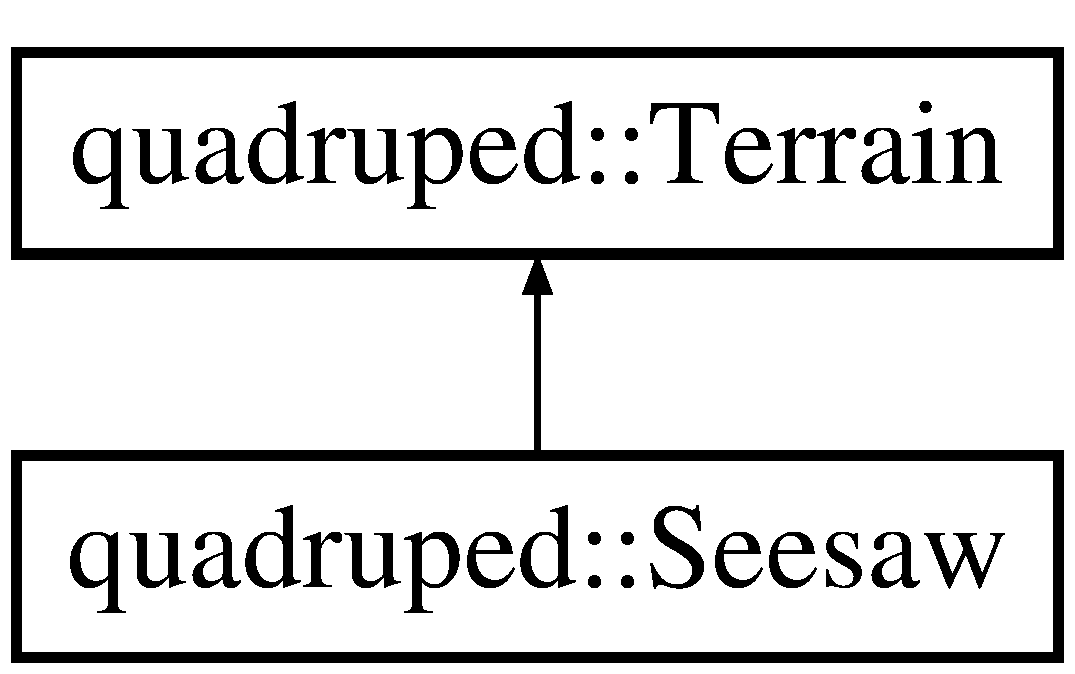
\includegraphics[height=2.000000cm]{classquadruped_1_1Seesaw}
\end{center}
\end{figure}
\subsection*{Public 成员函数}
\begin{DoxyCompactItemize}
\item 
\mbox{\Hypertarget{classquadruped_1_1Seesaw_a81c9e3f01fa0f40d3d1264cb4e5f9783}\label{classquadruped_1_1Seesaw_a81c9e3f01fa0f40d3d1264cb4e5f9783}} 
\hyperlink{classquadruped_1_1Seesaw_a81c9e3f01fa0f40d3d1264cb4e5f9783}{Seesaw} (void)
\begin{DoxyCompactList}\small\item\em Seesaw类的构造函数，完成地形标识符的初始化 \end{DoxyCompactList}\item 
virtual double \hyperlink{classquadruped_1_1Seesaw_ae3c06febd15cbab4d1ecaaef80f0e90e}{Get\+Hight} (double p\+\_\+x, double p\+\_\+y) override
\begin{DoxyCompactList}\small\item\em 获取当前地形在世界坐标系下的高度 \end{DoxyCompactList}\item 
virtual void \hyperlink{classquadruped_1_1Seesaw_afe71a03188bcc6bbd385356f8c5d10b3}{Updata\+Edge} (double p\+\_\+first\+\_\+edge\+\_\+\+D\+\_\+x, double p\+\_\+first\+\_\+edge\+\_\+\+D\+\_\+y) override
\begin{DoxyCompactList}\small\item\em 获取跷跷板与地面的交线中点在世界坐标系下的位置 \end{DoxyCompactList}\item 
virtual \hyperlink{cppTypes_8h_a65c27bf97693676535dd0b30ea0ad399}{Vec3}$<$ double $>$ \hyperlink{classquadruped_1_1Seesaw_aba969bdf4ad8e7b4e3af146598926cce}{Get\+Normal\+Vector} (double p\+\_\+x, double p\+\_\+y) override
\begin{DoxyCompactList}\small\item\em 预留接口 $\vert$ 获取跷跷板某一点处的法向量 \end{DoxyCompactList}\end{DoxyCompactItemize}
\subsection*{额外继承的成员函数}


\subsection{详细描述}
跷跷板类子类 

\subsection{成员函数说明}
\mbox{\Hypertarget{classquadruped_1_1Seesaw_ae3c06febd15cbab4d1ecaaef80f0e90e}\label{classquadruped_1_1Seesaw_ae3c06febd15cbab4d1ecaaef80f0e90e}} 
\index{quadruped\+::\+Seesaw@{quadruped\+::\+Seesaw}!Get\+Hight@{Get\+Hight}}
\index{Get\+Hight@{Get\+Hight}!quadruped\+::\+Seesaw@{quadruped\+::\+Seesaw}}
\subsubsection{\texorpdfstring{Get\+Hight()}{GetHight()}}
{\footnotesize\ttfamily double Seesaw\+::\+Get\+Hight (\begin{DoxyParamCaption}\item[{double}]{p\+\_\+x,  }\item[{double}]{p\+\_\+y }\end{DoxyParamCaption})\hspace{0.3cm}{\ttfamily [override]}, {\ttfamily [virtual]}}



获取当前地形在世界坐标系下的高度 


\begin{DoxyParams}{参数}
{\em p\+\_\+x} & 当前点在世界坐标系位置坐标的\+X值 \\
\hline
{\em p\+\_\+y} & 当前点在世界坐标系位置坐标的\+Y值 \\
\hline
\end{DoxyParams}
\begin{DoxyReturn}{返回}
double 
\end{DoxyReturn}


重载 \hyperlink{classquadruped_1_1Terrain}{quadruped\+::\+Terrain} .

\mbox{\Hypertarget{classquadruped_1_1Seesaw_aba969bdf4ad8e7b4e3af146598926cce}\label{classquadruped_1_1Seesaw_aba969bdf4ad8e7b4e3af146598926cce}} 
\index{quadruped\+::\+Seesaw@{quadruped\+::\+Seesaw}!Get\+Normal\+Vector@{Get\+Normal\+Vector}}
\index{Get\+Normal\+Vector@{Get\+Normal\+Vector}!quadruped\+::\+Seesaw@{quadruped\+::\+Seesaw}}
\subsubsection{\texorpdfstring{Get\+Normal\+Vector()}{GetNormalVector()}}
{\footnotesize\ttfamily \hyperlink{cppTypes_8h_a65c27bf97693676535dd0b30ea0ad399}{Vec3}$<$ double $>$ Seesaw\+::\+Get\+Normal\+Vector (\begin{DoxyParamCaption}\item[{double}]{p\+\_\+x,  }\item[{double}]{p\+\_\+y }\end{DoxyParamCaption})\hspace{0.3cm}{\ttfamily [override]}, {\ttfamily [virtual]}}



预留接口 $\vert$ 获取跷跷板某一点处的法向量 


\begin{DoxyParams}{参数}
{\em p\+\_\+x} & \\
\hline
{\em p\+\_\+y} & \\
\hline
\end{DoxyParams}
\begin{DoxyReturn}{返回}
Vec3$<$double$>$ 
\end{DoxyReturn}


实现了 \hyperlink{classquadruped_1_1Terrain}{quadruped\+::\+Terrain}.

\mbox{\Hypertarget{classquadruped_1_1Seesaw_afe71a03188bcc6bbd385356f8c5d10b3}\label{classquadruped_1_1Seesaw_afe71a03188bcc6bbd385356f8c5d10b3}} 
\index{quadruped\+::\+Seesaw@{quadruped\+::\+Seesaw}!Updata\+Edge@{Updata\+Edge}}
\index{Updata\+Edge@{Updata\+Edge}!quadruped\+::\+Seesaw@{quadruped\+::\+Seesaw}}
\subsubsection{\texorpdfstring{Updata\+Edge()}{UpdataEdge()}}
{\footnotesize\ttfamily void Seesaw\+::\+Updata\+Edge (\begin{DoxyParamCaption}\item[{double}]{p\+\_\+first\+\_\+edge\+\_\+\+D\+\_\+x,  }\item[{double}]{p\+\_\+first\+\_\+edge\+\_\+\+D\+\_\+y }\end{DoxyParamCaption})\hspace{0.3cm}{\ttfamily [override]}, {\ttfamily [virtual]}}



获取跷跷板与地面的交线中点在世界坐标系下的位置 


\begin{DoxyParams}{参数}
{\em p\+\_\+first\+\_\+edge\+\_\+\+D\+\_\+x} & 当前点在世界坐标系位置坐标的\+X值 \\
\hline
{\em p\+\_\+first\+\_\+edge\+\_\+\+D\+\_\+y} & 当前点在世界坐标系位置坐标的\+Y值 \\
\hline
\end{DoxyParams}


重载 \hyperlink{classquadruped_1_1Terrain}{quadruped\+::\+Terrain} .



参考 quadruped\+::\+Terrain\+::first\+\_\+edge\+\_\+\+D\+\_\+x , 以及 quadruped\+::\+Terrain\+::first\+\_\+edge\+\_\+\+D\+\_\+y.



该类的文档由以下文件生成\+:\begin{DoxyCompactItemize}
\item 
controller/motion\+Plan/terrain/\hyperlink{terrain_8hpp}{terrain.\+hpp}\item 
controller/motion\+Plan/terrain/\hyperlink{terrain_8cpp}{terrain.\+cpp}\end{DoxyCompactItemize}

\hypertarget{classquadruped_1_1Sill}{}\section{quadruped\+:\+:Sill类 参考}
\label{classquadruped_1_1Sill}\index{quadruped\+::\+Sill@{quadruped\+::\+Sill}}


门槛类子类  




{\ttfamily \#include $<$terrain.\+hpp$>$}

类 quadruped\+:\+:Sill 继承关系图\+:\begin{figure}[H]
\begin{center}
\leavevmode
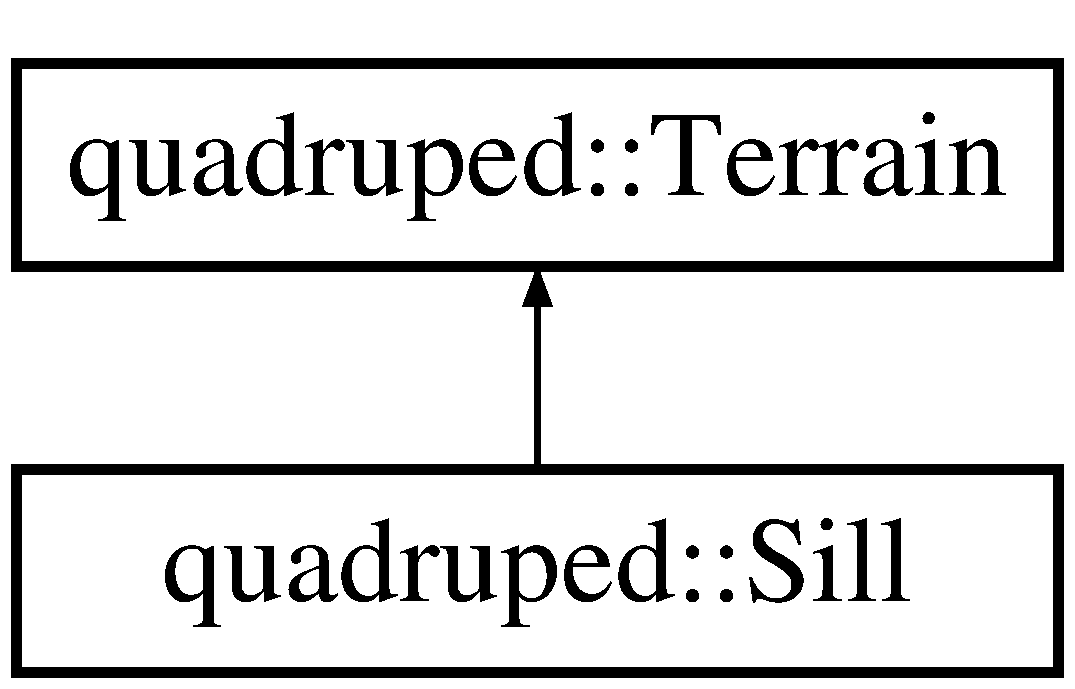
\includegraphics[height=2.000000cm]{classquadruped_1_1Sill}
\end{center}
\end{figure}
\subsection*{Public 成员函数}
\begin{DoxyCompactItemize}
\item 
\mbox{\Hypertarget{classquadruped_1_1Sill_a7e06ad0463b7a93a63d42aef3920f309}\label{classquadruped_1_1Sill_a7e06ad0463b7a93a63d42aef3920f309}} 
\hyperlink{classquadruped_1_1Sill_a7e06ad0463b7a93a63d42aef3920f309}{Sill} (void)
\begin{DoxyCompactList}\small\item\em Sill类的构造函数，完成地形标识符以及地形分割线的初始化 \end{DoxyCompactList}\item 
virtual double \hyperlink{classquadruped_1_1Sill_ab128372a0914aef0c2665e71a059a615}{Get\+Hight} (double p\+\_\+x, double p\+\_\+y) override
\begin{DoxyCompactList}\small\item\em 获取当前地形在世界坐标系下的高度 \end{DoxyCompactList}\item 
virtual void \hyperlink{classquadruped_1_1Sill_adfcc36758c795efe14d355c5adbd2d0d}{Updata\+Edge} (double p\+\_\+first\+\_\+edge\+\_\+\+D\+\_\+x, double p\+\_\+first\+\_\+edge\+\_\+\+D\+\_\+y) override
\begin{DoxyCompactList}\small\item\em 获取门槛轴线中点在世界坐标系下的位置以及分割线和危险区的设置 \end{DoxyCompactList}\item 
virtual \hyperlink{cppTypes_8h_a65c27bf97693676535dd0b30ea0ad399}{Vec3}$<$ double $>$ \hyperlink{classquadruped_1_1Sill_a27ad935cad8d7be75991a287c2de5283}{Get\+Normal\+Vector} (double p\+\_\+x, double p\+\_\+y) override
\begin{DoxyCompactList}\small\item\em 预留接口 $\vert$ 获取门槛某一点处的法向量 \end{DoxyCompactList}\end{DoxyCompactItemize}
\subsection*{额外继承的成员函数}


\subsection{详细描述}
门槛类子类 

\subsection{成员函数说明}
\mbox{\Hypertarget{classquadruped_1_1Sill_ab128372a0914aef0c2665e71a059a615}\label{classquadruped_1_1Sill_ab128372a0914aef0c2665e71a059a615}} 
\index{quadruped\+::\+Sill@{quadruped\+::\+Sill}!Get\+Hight@{Get\+Hight}}
\index{Get\+Hight@{Get\+Hight}!quadruped\+::\+Sill@{quadruped\+::\+Sill}}
\subsubsection{\texorpdfstring{Get\+Hight()}{GetHight()}}
{\footnotesize\ttfamily double Sill\+::\+Get\+Hight (\begin{DoxyParamCaption}\item[{double}]{p\+\_\+x,  }\item[{double}]{p\+\_\+y }\end{DoxyParamCaption})\hspace{0.3cm}{\ttfamily [override]}, {\ttfamily [virtual]}}



获取当前地形在世界坐标系下的高度 


\begin{DoxyParams}{参数}
{\em p\+\_\+x} & 当前点在世界坐标系位置坐标的\+X值 \\
\hline
{\em p\+\_\+y} & 当前点在世界坐标系位置坐标的\+Y值 \\
\hline
\end{DoxyParams}
\begin{DoxyReturn}{返回}
double 
\end{DoxyReturn}


重载 \hyperlink{classquadruped_1_1Terrain}{quadruped\+::\+Terrain} .

\mbox{\Hypertarget{classquadruped_1_1Sill_a27ad935cad8d7be75991a287c2de5283}\label{classquadruped_1_1Sill_a27ad935cad8d7be75991a287c2de5283}} 
\index{quadruped\+::\+Sill@{quadruped\+::\+Sill}!Get\+Normal\+Vector@{Get\+Normal\+Vector}}
\index{Get\+Normal\+Vector@{Get\+Normal\+Vector}!quadruped\+::\+Sill@{quadruped\+::\+Sill}}
\subsubsection{\texorpdfstring{Get\+Normal\+Vector()}{GetNormalVector()}}
{\footnotesize\ttfamily \hyperlink{cppTypes_8h_a65c27bf97693676535dd0b30ea0ad399}{Vec3}$<$ double $>$ Sill\+::\+Get\+Normal\+Vector (\begin{DoxyParamCaption}\item[{double}]{p\+\_\+x,  }\item[{double}]{p\+\_\+y }\end{DoxyParamCaption})\hspace{0.3cm}{\ttfamily [override]}, {\ttfamily [virtual]}}



预留接口 $\vert$ 获取门槛某一点处的法向量 


\begin{DoxyParams}{参数}
{\em p\+\_\+x} & \\
\hline
{\em p\+\_\+y} & \\
\hline
\end{DoxyParams}
\begin{DoxyReturn}{返回}
Vec3$<$double$>$ 
\end{DoxyReturn}


实现了 \hyperlink{classquadruped_1_1Terrain}{quadruped\+::\+Terrain}.

\mbox{\Hypertarget{classquadruped_1_1Sill_adfcc36758c795efe14d355c5adbd2d0d}\label{classquadruped_1_1Sill_adfcc36758c795efe14d355c5adbd2d0d}} 
\index{quadruped\+::\+Sill@{quadruped\+::\+Sill}!Updata\+Edge@{Updata\+Edge}}
\index{Updata\+Edge@{Updata\+Edge}!quadruped\+::\+Sill@{quadruped\+::\+Sill}}
\subsubsection{\texorpdfstring{Updata\+Edge()}{UpdataEdge()}}
{\footnotesize\ttfamily void Sill\+::\+Updata\+Edge (\begin{DoxyParamCaption}\item[{double}]{p\+\_\+first\+\_\+edge\+\_\+\+D\+\_\+x,  }\item[{double}]{p\+\_\+first\+\_\+edge\+\_\+\+D\+\_\+y }\end{DoxyParamCaption})\hspace{0.3cm}{\ttfamily [override]}, {\ttfamily [virtual]}}



获取门槛轴线中点在世界坐标系下的位置以及分割线和危险区的设置 


\begin{DoxyParams}{参数}
{\em p\+\_\+first\+\_\+edge\+\_\+\+D\+\_\+x} & 当前点在世界坐标系位置坐标的\+X值 \\
\hline
{\em p\+\_\+first\+\_\+edge\+\_\+\+D\+\_\+y} & 当前点在世界坐标系位置坐标的\+Y值 \\
\hline
\end{DoxyParams}


重载 \hyperlink{classquadruped_1_1Terrain}{quadruped\+::\+Terrain} .



参考 quadruped\+::\+Terrain\+::average\+Danger\+Area, quadruped\+::\+Terrain\+::first\+\_\+edge\+\_\+\+D\+\_\+x, quadruped\+::\+Terrain\+::first\+\_\+edge\+\_\+\+D\+\_\+y, L\+I\+M\+I\+T\+\_\+\+I\+N\+F\+I\+N\+I\+TE, quadruped\+::\+Terrain\+::num\+Split, quadruped\+::\+Terrain\+::safe\+Area, S\+I\+L\+L\+\_\+\+W\+I\+D\+TH , 以及 quadruped\+::\+Terrain\+::split.



该类的文档由以下文件生成\+:\begin{DoxyCompactItemize}
\item 
controller/motion\+Plan/terrain/\hyperlink{terrain_8hpp}{terrain.\+hpp}\item 
controller/motion\+Plan/terrain/\hyperlink{terrain_8cpp}{terrain.\+cpp}\end{DoxyCompactItemize}

\hypertarget{classquadruped_1_1SingleContact}{}\section{quadruped\+:\+:Single\+Contact类 参考}
\label{classquadruped_1_1SingleContact}\index{quadruped\+::\+Single\+Contact@{quadruped\+::\+Single\+Contact}}
类 quadruped\+:\+:Single\+Contact 继承关系图\+:\begin{figure}[H]
\begin{center}
\leavevmode
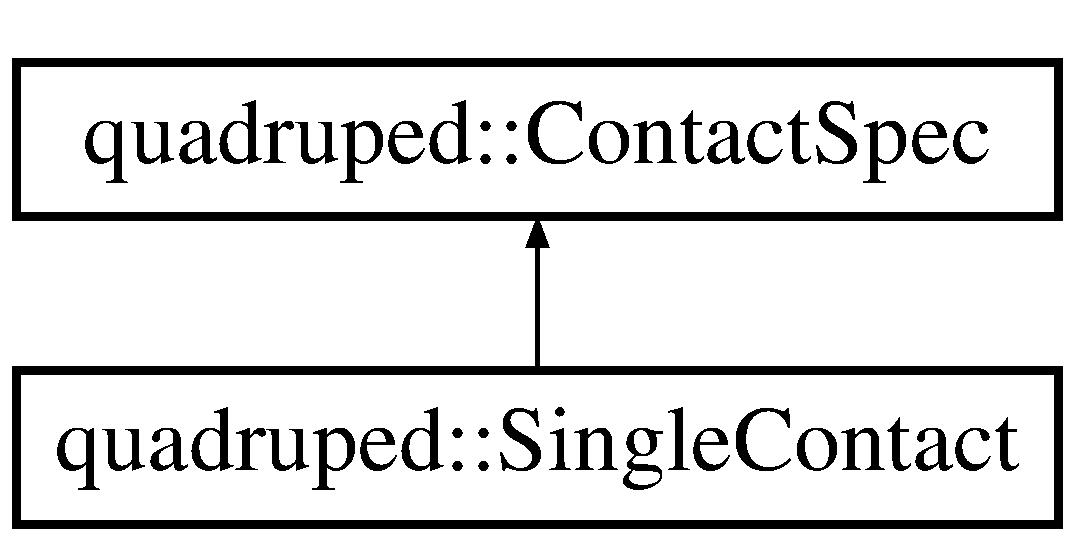
\includegraphics[height=2.000000cm]{classquadruped_1_1SingleContact}
\end{center}
\end{figure}
\subsection*{Public 成员函数}
\begin{DoxyCompactItemize}
\item 
\mbox{\Hypertarget{classquadruped_1_1SingleContact_a62aa4cde629fe07e2dd9fea782467b6b}\label{classquadruped_1_1SingleContact_a62aa4cde629fe07e2dd9fea782467b6b}} 
{\bfseries Single\+Contact} (\hyperlink{classquadruped_1_1RobotModel}{Robot\+Model} $\ast$p\+\_\+robot\+Model, const int p\+\_\+link\+Id)
\item 
\mbox{\Hypertarget{classquadruped_1_1SingleContact_a0ffd7efa12238fe73ff50b6e1a4ac99a}\label{classquadruped_1_1SingleContact_a0ffd7efa12238fe73ff50b6e1a4ac99a}} 
virtual bool {\bfseries Update\+Jc} ()
\item 
\mbox{\Hypertarget{classquadruped_1_1SingleContact_a7b261c132fb5b27e21b85bc444d25217}\label{classquadruped_1_1SingleContact_a7b261c132fb5b27e21b85bc444d25217}} 
virtual bool {\bfseries Update\+Jc\+Dot\+Qdot} ()
\item 
\mbox{\Hypertarget{classquadruped_1_1SingleContact_af229c4fb6f373bba6079fd823921ec08}\label{classquadruped_1_1SingleContact_af229c4fb6f373bba6079fd823921ec08}} 
virtual bool {\bfseries Update\+Uf} ()
\item 
\mbox{\Hypertarget{classquadruped_1_1SingleContact_abf288d687c3c41c0f08cfff0541c56c3}\label{classquadruped_1_1SingleContact_abf288d687c3c41c0f08cfff0541c56c3}} 
virtual bool {\bfseries Update\+Inequality\+Vector} ()
\end{DoxyCompactItemize}
\subsection*{Public 属性}
\begin{DoxyCompactItemize}
\item 
\mbox{\Hypertarget{classquadruped_1_1SingleContact_a35f81f35c29337a40a3643280c2b354e}\label{classquadruped_1_1SingleContact_a35f81f35c29337a40a3643280c2b354e}} 
\hyperlink{classquadruped_1_1RobotModel}{Robot\+Model} $\ast$ {\bfseries robot\+Model}
\item 
\mbox{\Hypertarget{classquadruped_1_1SingleContact_aec067d7497b9288aec37a0a2bd22336c}\label{classquadruped_1_1SingleContact_aec067d7497b9288aec37a0a2bd22336c}} 
int {\bfseries contact\+\_\+id}
\item 
\mbox{\Hypertarget{classquadruped_1_1SingleContact_afeca70250ce010f100d435143de156e5}\label{classquadruped_1_1SingleContact_afeca70250ce010f100d435143de156e5}} 
int {\bfseries dim\+\_\+cstr}
\end{DoxyCompactItemize}
\subsection*{额外继承的成员函数}


该类的文档由以下文件生成\+:\begin{DoxyCompactItemize}
\item 
controller/wbc/contact/single\+Contact.\+hpp\item 
controller/wbc/contact/\hyperlink{singleContact_8cpp}{single\+Contact.\+cpp}\end{DoxyCompactItemize}

\hypertarget{classquadruped_1_1SingleLeg}{}\section{quadruped\+:\+:Single\+Leg类 参考}
\label{classquadruped_1_1SingleLeg}\index{quadruped\+::\+Single\+Leg@{quadruped\+::\+Single\+Leg}}


Actiger单腿控制器  




{\ttfamily \#include $<$single\+Leg\+Control.\+hpp$>$}

\subsection*{Public 成员函数}
\begin{DoxyCompactItemize}
\item 
\hyperlink{classquadruped_1_1SingleLeg_a3517b91ff7317237d4e7e6713ef31d83}{Single\+Leg} (\hyperlink{classquadruped_1_1LegStateEstimate}{Leg\+State\+Estimate} $\ast$p\+\_\+leg\+Stste, \hyperlink{classquadruped_1_1Parameters}{Parameters} $\ast$p\+\_\+para)
\begin{DoxyCompactList}\small\item\em Single\+Leg类的构造函数，完成所有对象成员的初始化 \end{DoxyCompactList}\item 
\mbox{\Hypertarget{classquadruped_1_1SingleLeg_af7d1589824b4714abbd3bcfa11099056}\label{classquadruped_1_1SingleLeg_af7d1589824b4714abbd3bcfa11099056}} 
virtual \hyperlink{classquadruped_1_1SingleLeg_af7d1589824b4714abbd3bcfa11099056}{$\sim$\+Single\+Leg} (void)
\begin{DoxyCompactList}\small\item\em Single\+Leg类的析构函数 \end{DoxyCompactList}\item 
\hyperlink{structlegTorque__t}{leg\+Torque\+\_\+t} \hyperlink{classquadruped_1_1SingleLeg_a2162ecb433c3583bf3c3ca1289dc9472}{Single\+Stance\+Control} (\hyperlink{cppTypes_8h_adb7d462b35d31f0b2583b3e230a2a2c3}{Mat3}$<$ double $>$ p\+\_\+rotation, \hyperlink{cppTypes_8h_a65c27bf97693676535dd0b30ea0ad399}{Vec3}$<$ double $>$ p\+\_\+grav, \hyperlink{cppTypes_8h_a65c27bf97693676535dd0b30ea0ad399}{Vec3}$<$ double $>$ coriolis, \hyperlink{cppTypes_8h_a65c27bf97693676535dd0b30ea0ad399}{Vec3}$<$ double $>$ p\+\_\+react\+Force)
\begin{DoxyCompactList}\small\item\em Actiger支撑腿控制函数 \end{DoxyCompactList}\item 
\hyperlink{structlegTorque__t}{leg\+Torque\+\_\+t} \hyperlink{classquadruped_1_1SingleLeg_a222857a901318676d20d34581fd7504a}{Single\+Swing\+Control} (\hyperlink{cppTypes_8h_adb7d462b35d31f0b2583b3e230a2a2c3}{Mat3}$<$ double $>$ p\+\_\+rotation, \hyperlink{cppTypes_8h_a65c27bf97693676535dd0b30ea0ad399}{Vec3}$<$ double $>$ p\+\_\+grav, \hyperlink{cppTypes_8h_a65c27bf97693676535dd0b30ea0ad399}{Vec3}$<$ double $>$ coriolis, \hyperlink{cppTypes_8h_a65c27bf97693676535dd0b30ea0ad399}{Vec3}$<$ double $>$ p\+\_\+des\+Pos, \hyperlink{cppTypes_8h_a65c27bf97693676535dd0b30ea0ad399}{Vec3}$<$ double $>$ p\+\_\+des\+Vel)
\begin{DoxyCompactList}\small\item\em Actiger摆动腿控制函数 \end{DoxyCompactList}\end{DoxyCompactItemize}
\subsection*{Public 属性}
\begin{DoxyCompactItemize}
\item 
\mbox{\Hypertarget{classquadruped_1_1SingleLeg_aaf4f8f8686ef952a15236892e7eacfd2}\label{classquadruped_1_1SingleLeg_aaf4f8f8686ef952a15236892e7eacfd2}} 
\hyperlink{cppTypes_8h_a65c27bf97693676535dd0b30ea0ad399}{Vec3}$<$ double $>$ \hyperlink{classquadruped_1_1SingleLeg_aaf4f8f8686ef952a15236892e7eacfd2}{torque\+Feed\+Forward}
\begin{DoxyCompactList}\small\item\em W\+B\+C预留接口 \end{DoxyCompactList}\item 
\mbox{\Hypertarget{classquadruped_1_1SingleLeg_a7463a742fbf6923728c4761393aa68e0}\label{classquadruped_1_1SingleLeg_a7463a742fbf6923728c4761393aa68e0}} 
\hyperlink{cppTypes_8h_a65c27bf97693676535dd0b30ea0ad399}{Vec3}$<$ double $>$ \hyperlink{classquadruped_1_1SingleLeg_a7463a742fbf6923728c4761393aa68e0}{q\+Des}
\begin{DoxyCompactList}\small\item\em W\+B\+C预留接口 \end{DoxyCompactList}\item 
\mbox{\Hypertarget{classquadruped_1_1SingleLeg_a086eb6cdde5bf9583a244d1fd2f7d803}\label{classquadruped_1_1SingleLeg_a086eb6cdde5bf9583a244d1fd2f7d803}} 
\hyperlink{cppTypes_8h_a65c27bf97693676535dd0b30ea0ad399}{Vec3}$<$ double $>$ \hyperlink{classquadruped_1_1SingleLeg_a086eb6cdde5bf9583a244d1fd2f7d803}{qd\+Des}
\begin{DoxyCompactList}\small\item\em W\+B\+C预留接口 \end{DoxyCompactList}\item 
\mbox{\Hypertarget{classquadruped_1_1SingleLeg_a2166770aa38c23e6ae2d07e1b8fc5aca}\label{classquadruped_1_1SingleLeg_a2166770aa38c23e6ae2d07e1b8fc5aca}} 
\hyperlink{classquadruped_1_1LegStateEstimate}{Leg\+State\+Estimate} $\ast$ \hyperlink{classquadruped_1_1SingleLeg_a2166770aa38c23e6ae2d07e1b8fc5aca}{leg\+Stste}
\begin{DoxyCompactList}\small\item\em Leg\+State\+Estimate类的实例化对象，存储机器人单腿状态信息 \end{DoxyCompactList}\item 
\mbox{\Hypertarget{classquadruped_1_1SingleLeg_ab3d1405314c2206d8b76413e7dd9268a}\label{classquadruped_1_1SingleLeg_ab3d1405314c2206d8b76413e7dd9268a}} 
\hyperlink{classquadruped_1_1Parameters}{Parameters} $\ast$ \hyperlink{classquadruped_1_1SingleLeg_ab3d1405314c2206d8b76413e7dd9268a}{para}
\begin{DoxyCompactList}\small\item\em Parameters类的实例化对象，存储一些被频繁使用的参数 \end{DoxyCompactList}\end{DoxyCompactItemize}


\subsection{详细描述}
Actiger单腿控制器 

\subsection{构造及析构函数说明}
\mbox{\Hypertarget{classquadruped_1_1SingleLeg_a3517b91ff7317237d4e7e6713ef31d83}\label{classquadruped_1_1SingleLeg_a3517b91ff7317237d4e7e6713ef31d83}} 
\index{quadruped\+::\+Single\+Leg@{quadruped\+::\+Single\+Leg}!Single\+Leg@{Single\+Leg}}
\index{Single\+Leg@{Single\+Leg}!quadruped\+::\+Single\+Leg@{quadruped\+::\+Single\+Leg}}
\subsubsection{\texorpdfstring{Single\+Leg()}{SingleLeg()}}
{\footnotesize\ttfamily Single\+Leg\+::\+Single\+Leg (\begin{DoxyParamCaption}\item[{\hyperlink{classquadruped_1_1LegStateEstimate}{Leg\+State\+Estimate} $\ast$}]{p\+\_\+leg\+Stste,  }\item[{\hyperlink{classquadruped_1_1Parameters}{Parameters} $\ast$}]{p\+\_\+para }\end{DoxyParamCaption})\hspace{0.3cm}{\ttfamily [explicit]}}



Single\+Leg类的构造函数，完成所有对象成员的初始化 


\begin{DoxyParams}{参数}
{\em p\+\_\+leg\+Stste} & Leg\+State\+Estimate类的实例化对象，存储机器人单腿状态信息，用来初始化对象成员leg\+Stste \\
\hline
{\em p\+\_\+para} & Parameters类的实例化对象，存储一些被频繁使用的参数，用来初始化对象成员para \\
\hline
\end{DoxyParams}


参考 leg\+Stste , 以及 para.



\subsection{成员函数说明}
\mbox{\Hypertarget{classquadruped_1_1SingleLeg_a2162ecb433c3583bf3c3ca1289dc9472}\label{classquadruped_1_1SingleLeg_a2162ecb433c3583bf3c3ca1289dc9472}} 
\index{quadruped\+::\+Single\+Leg@{quadruped\+::\+Single\+Leg}!Single\+Stance\+Control@{Single\+Stance\+Control}}
\index{Single\+Stance\+Control@{Single\+Stance\+Control}!quadruped\+::\+Single\+Leg@{quadruped\+::\+Single\+Leg}}
\subsubsection{\texorpdfstring{Single\+Stance\+Control()}{SingleStanceControl()}}
{\footnotesize\ttfamily \hyperlink{structlegTorque__t}{leg\+Torque\+\_\+t} Single\+Leg\+::\+Single\+Stance\+Control (\begin{DoxyParamCaption}\item[{\hyperlink{cppTypes_8h_adb7d462b35d31f0b2583b3e230a2a2c3}{Mat3}$<$ double $>$}]{p\+\_\+rotation,  }\item[{\hyperlink{cppTypes_8h_a65c27bf97693676535dd0b30ea0ad399}{Vec3}$<$ double $>$}]{p\+\_\+grav,  }\item[{\hyperlink{cppTypes_8h_a65c27bf97693676535dd0b30ea0ad399}{Vec3}$<$ double $>$}]{coriolis,  }\item[{\hyperlink{cppTypes_8h_a65c27bf97693676535dd0b30ea0ad399}{Vec3}$<$ double $>$}]{p\+\_\+react\+Force }\end{DoxyParamCaption})}



Actiger支撑腿控制函数 


\begin{DoxyParams}{参数}
{\em p\+\_\+rotation} & 惯性坐标系到机体坐标系的旋转矩阵 \\
\hline
{\em p\+\_\+grav} & 拉格朗日动力学方程中的重力项 \\
\hline
{\em coriolis} & 拉格朗日动力学方程中的离心力-\/哥氏力项 \\
\hline
{\em p\+\_\+react\+Force} & Actiger模型预测控制器计算得到的地面反作用力\mbox{[}G\+RF\mbox{]} \\
\hline
\end{DoxyParams}
\begin{DoxyReturn}{返回}
\hyperlink{structlegTorque__t}{leg\+Torque\+\_\+t} 
\end{DoxyReturn}


参考 quadruped\+::\+Leg\+State\+Estimate\+::jacobian , 以及 leg\+Stste.



参考自 quadruped\+::\+Leg\+Control\+::\+Leg\+Joint\+Control().

\mbox{\Hypertarget{classquadruped_1_1SingleLeg_a222857a901318676d20d34581fd7504a}\label{classquadruped_1_1SingleLeg_a222857a901318676d20d34581fd7504a}} 
\index{quadruped\+::\+Single\+Leg@{quadruped\+::\+Single\+Leg}!Single\+Swing\+Control@{Single\+Swing\+Control}}
\index{Single\+Swing\+Control@{Single\+Swing\+Control}!quadruped\+::\+Single\+Leg@{quadruped\+::\+Single\+Leg}}
\subsubsection{\texorpdfstring{Single\+Swing\+Control()}{SingleSwingControl()}}
{\footnotesize\ttfamily \hyperlink{structlegTorque__t}{leg\+Torque\+\_\+t} Single\+Leg\+::\+Single\+Swing\+Control (\begin{DoxyParamCaption}\item[{\hyperlink{cppTypes_8h_adb7d462b35d31f0b2583b3e230a2a2c3}{Mat3}$<$ double $>$}]{p\+\_\+rotation,  }\item[{\hyperlink{cppTypes_8h_a65c27bf97693676535dd0b30ea0ad399}{Vec3}$<$ double $>$}]{p\+\_\+grav,  }\item[{\hyperlink{cppTypes_8h_a65c27bf97693676535dd0b30ea0ad399}{Vec3}$<$ double $>$}]{coriolis,  }\item[{\hyperlink{cppTypes_8h_a65c27bf97693676535dd0b30ea0ad399}{Vec3}$<$ double $>$}]{p\+\_\+des\+Pos,  }\item[{\hyperlink{cppTypes_8h_a65c27bf97693676535dd0b30ea0ad399}{Vec3}$<$ double $>$}]{p\+\_\+des\+Vel }\end{DoxyParamCaption})}



Actiger摆动腿控制函数 


\begin{DoxyParams}{参数}
{\em p\+\_\+rotation} & 惯性坐标系到机体坐标系的旋转矩阵 \\
\hline
{\em p\+\_\+grav} & 拉格朗日动力学方程中的重力项 \\
\hline
{\em coriolis} & 拉格朗日动力学方程中的离心力-\/哥氏力项 \\
\hline
{\em p\+\_\+des\+Pos} & 摆动腿足端在机体坐标系下的期望位置 \\
\hline
{\em p\+\_\+des\+Vel} & 摆动腿足端在机体坐标系下的期望速度 \\
\hline
\end{DoxyParams}
\begin{DoxyReturn}{返回}
\hyperlink{structlegTorque__t}{leg\+Torque\+\_\+t} 
\end{DoxyReturn}


参考 quadruped\+::\+Leg\+State\+Estimate\+::endfoot\+\_\+hip, quadruped\+::\+Leg\+State\+Estimate\+::endfoot\+\_\+vel\+\_\+hip, quadruped\+::\+Leg\+State\+Estimate\+::hip\+\_\+pos\+\_\+body, quadruped\+::\+Leg\+State\+Estimate\+::jacobian, quadruped\+::\+Parameters\+::leg\+\_\+kd\+Joint, quadruped\+::\+Parameters\+::leg\+\_\+kp\+Joint, leg\+Stste , 以及 para.



参考自 quadruped\+::\+Leg\+Control\+::\+Leg\+Joint\+Control().



该类的文档由以下文件生成\+:\begin{DoxyCompactItemize}
\item 
controller/leg\+Controller/\hyperlink{singleLegControl_8hpp}{single\+Leg\+Control.\+hpp}\item 
controller/leg\+Controller/\hyperlink{singleLegControl_8cpp}{single\+Leg\+Control.\+cpp}\end{DoxyCompactItemize}

\hypertarget{classquadruped_1_1Slope}{}\section{quadruped\+:\+:Slope类 参考}
\label{classquadruped_1_1Slope}\index{quadruped\+::\+Slope@{quadruped\+::\+Slope}}


坡面类子类  




{\ttfamily \#include $<$terrain.\+hpp$>$}

类 quadruped\+:\+:Slope 继承关系图\+:\begin{figure}[H]
\begin{center}
\leavevmode
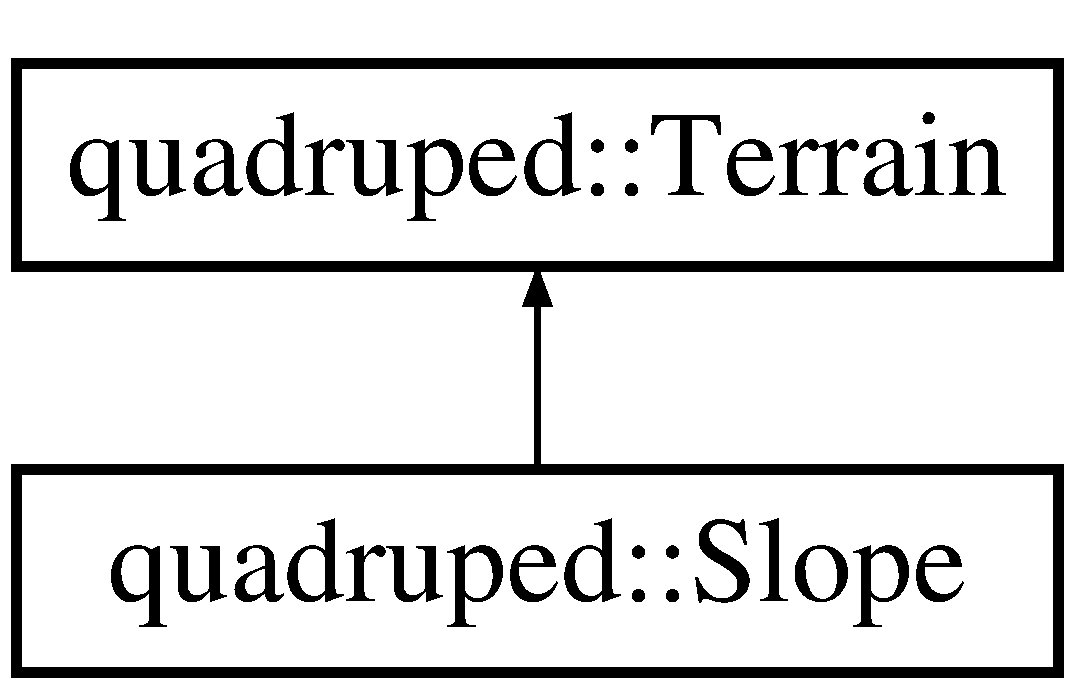
\includegraphics[height=2.000000cm]{classquadruped_1_1Slope}
\end{center}
\end{figure}
\subsection*{Public 成员函数}
\begin{DoxyCompactItemize}
\item 
\mbox{\Hypertarget{classquadruped_1_1Slope_a21274f08f8ab6b2063f13b92b8e9ccec}\label{classquadruped_1_1Slope_a21274f08f8ab6b2063f13b92b8e9ccec}} 
\hyperlink{classquadruped_1_1Slope_a21274f08f8ab6b2063f13b92b8e9ccec}{Slope} (void)
\begin{DoxyCompactList}\small\item\em Slope类的构造函数，完成地形标识符以及地形分割线的初始化 \end{DoxyCompactList}\item 
virtual double \hyperlink{classquadruped_1_1Slope_a964d5d93a7f650eaaa10028a17cc81a4}{Get\+Hight} (double p\+\_\+x, double p\+\_\+y) override
\begin{DoxyCompactList}\small\item\em 获取当前地形在世界坐标系下的高度 \end{DoxyCompactList}\item 
virtual void \hyperlink{classquadruped_1_1Slope_a696cc67c45bff48601eeaa56a54d87f7}{Updata\+Edge} (double p\+\_\+first\+\_\+edge\+\_\+\+D\+\_\+x, double p\+\_\+first\+\_\+edge\+\_\+\+D\+\_\+y) override
\begin{DoxyCompactList}\small\item\em 获取坡面与地面的交线中点在世界坐标系下的位置 \end{DoxyCompactList}\item 
virtual \hyperlink{cppTypes_8h_a65c27bf97693676535dd0b30ea0ad399}{Vec3}$<$ double $>$ \hyperlink{classquadruped_1_1Slope_aaa6bd2fa6b63c5c1b4b3172fd1a5bc0d}{Get\+Normal\+Vector} (double p\+\_\+x, double p\+\_\+y) override
\begin{DoxyCompactList}\small\item\em 预留接口 $\vert$ 获取坡面某一点处的法向量 \end{DoxyCompactList}\end{DoxyCompactItemize}
\subsection*{额外继承的成员函数}


\subsection{详细描述}
坡面类子类 

\subsection{成员函数说明}
\mbox{\Hypertarget{classquadruped_1_1Slope_a964d5d93a7f650eaaa10028a17cc81a4}\label{classquadruped_1_1Slope_a964d5d93a7f650eaaa10028a17cc81a4}} 
\index{quadruped\+::\+Slope@{quadruped\+::\+Slope}!Get\+Hight@{Get\+Hight}}
\index{Get\+Hight@{Get\+Hight}!quadruped\+::\+Slope@{quadruped\+::\+Slope}}
\subsubsection{\texorpdfstring{Get\+Hight()}{GetHight()}}
{\footnotesize\ttfamily double Slope\+::\+Get\+Hight (\begin{DoxyParamCaption}\item[{double}]{p\+\_\+x,  }\item[{double}]{p\+\_\+y }\end{DoxyParamCaption})\hspace{0.3cm}{\ttfamily [override]}, {\ttfamily [virtual]}}



获取当前地形在世界坐标系下的高度 


\begin{DoxyParams}{参数}
{\em p\+\_\+x} & 当前点在世界坐标系位置坐标的\+X值 \\
\hline
{\em p\+\_\+y} & 当前点在世界坐标系位置坐标的\+Y值 \\
\hline
\end{DoxyParams}
\begin{DoxyReturn}{返回}
double 
\end{DoxyReturn}


重载 \hyperlink{classquadruped_1_1Terrain}{quadruped\+::\+Terrain} .



参考 quadruped\+::\+Terrain\+::first\+\_\+edge\+\_\+\+D\+\_\+x, S\+L\+O\+P\+E\+\_\+\+D\+O\+W\+N\+\_\+\+A\+N\+G\+LE, S\+L\+O\+P\+E\+\_\+\+D\+O\+W\+N\+\_\+\+L\+E\+N\+G\+TH, S\+L\+O\+P\+E\+\_\+\+M\+I\+D\+\_\+\+H\+E\+I\+G\+HT, S\+L\+O\+P\+E\+\_\+\+M\+I\+D\+\_\+\+L\+E\+N\+G\+TH, S\+L\+O\+P\+E\+\_\+\+U\+P\+\_\+\+A\+N\+G\+LE , 以及 S\+L\+O\+P\+E\+\_\+\+U\+P\+\_\+\+L\+E\+N\+G\+TH.

\mbox{\Hypertarget{classquadruped_1_1Slope_aaa6bd2fa6b63c5c1b4b3172fd1a5bc0d}\label{classquadruped_1_1Slope_aaa6bd2fa6b63c5c1b4b3172fd1a5bc0d}} 
\index{quadruped\+::\+Slope@{quadruped\+::\+Slope}!Get\+Normal\+Vector@{Get\+Normal\+Vector}}
\index{Get\+Normal\+Vector@{Get\+Normal\+Vector}!quadruped\+::\+Slope@{quadruped\+::\+Slope}}
\subsubsection{\texorpdfstring{Get\+Normal\+Vector()}{GetNormalVector()}}
{\footnotesize\ttfamily \hyperlink{cppTypes_8h_a65c27bf97693676535dd0b30ea0ad399}{Vec3}$<$ double $>$ Slope\+::\+Get\+Normal\+Vector (\begin{DoxyParamCaption}\item[{double}]{p\+\_\+x,  }\item[{double}]{p\+\_\+y }\end{DoxyParamCaption})\hspace{0.3cm}{\ttfamily [override]}, {\ttfamily [virtual]}}



预留接口 $\vert$ 获取坡面某一点处的法向量 


\begin{DoxyParams}{参数}
{\em p\+\_\+x} & \\
\hline
{\em p\+\_\+y} & \\
\hline
\end{DoxyParams}
\begin{DoxyReturn}{返回}
Vec3$<$double$>$ 
\end{DoxyReturn}


实现了 \hyperlink{classquadruped_1_1Terrain}{quadruped\+::\+Terrain}.

\mbox{\Hypertarget{classquadruped_1_1Slope_a696cc67c45bff48601eeaa56a54d87f7}\label{classquadruped_1_1Slope_a696cc67c45bff48601eeaa56a54d87f7}} 
\index{quadruped\+::\+Slope@{quadruped\+::\+Slope}!Updata\+Edge@{Updata\+Edge}}
\index{Updata\+Edge@{Updata\+Edge}!quadruped\+::\+Slope@{quadruped\+::\+Slope}}
\subsubsection{\texorpdfstring{Updata\+Edge()}{UpdataEdge()}}
{\footnotesize\ttfamily void Slope\+::\+Updata\+Edge (\begin{DoxyParamCaption}\item[{double}]{p\+\_\+first\+\_\+edge\+\_\+\+D\+\_\+x,  }\item[{double}]{p\+\_\+first\+\_\+edge\+\_\+\+D\+\_\+y }\end{DoxyParamCaption})\hspace{0.3cm}{\ttfamily [override]}, {\ttfamily [virtual]}}



获取坡面与地面的交线中点在世界坐标系下的位置 


\begin{DoxyParams}{参数}
{\em p\+\_\+first\+\_\+edge\+\_\+\+D\+\_\+x} & 当前点在世界坐标系位置坐标的\+X值 \\
\hline
{\em p\+\_\+first\+\_\+edge\+\_\+\+D\+\_\+y} & 当前点在世界坐标系位置坐标的\+Y值 \\
\hline
\end{DoxyParams}


重载 \hyperlink{classquadruped_1_1Terrain}{quadruped\+::\+Terrain} .



参考 quadruped\+::\+Terrain\+::first\+\_\+edge\+\_\+\+D\+\_\+x , 以及 quadruped\+::\+Terrain\+::first\+\_\+edge\+\_\+\+D\+\_\+y.



该类的文档由以下文件生成\+:\begin{DoxyCompactItemize}
\item 
controller/motion\+Plan/terrain/\hyperlink{terrain_8hpp}{terrain.\+hpp}\item 
controller/motion\+Plan/terrain/\hyperlink{terrain_8cpp}{terrain.\+cpp}\end{DoxyCompactItemize}

\hypertarget{classquadruped_1_1Stage}{}\section{quadruped\+:\+:Stage类 参考}
\label{classquadruped_1_1Stage}\index{quadruped\+::\+Stage@{quadruped\+::\+Stage}}


平台类子类  




{\ttfamily \#include $<$terrain.\+hpp$>$}

类 quadruped\+:\+:Stage 继承关系图\+:\begin{figure}[H]
\begin{center}
\leavevmode
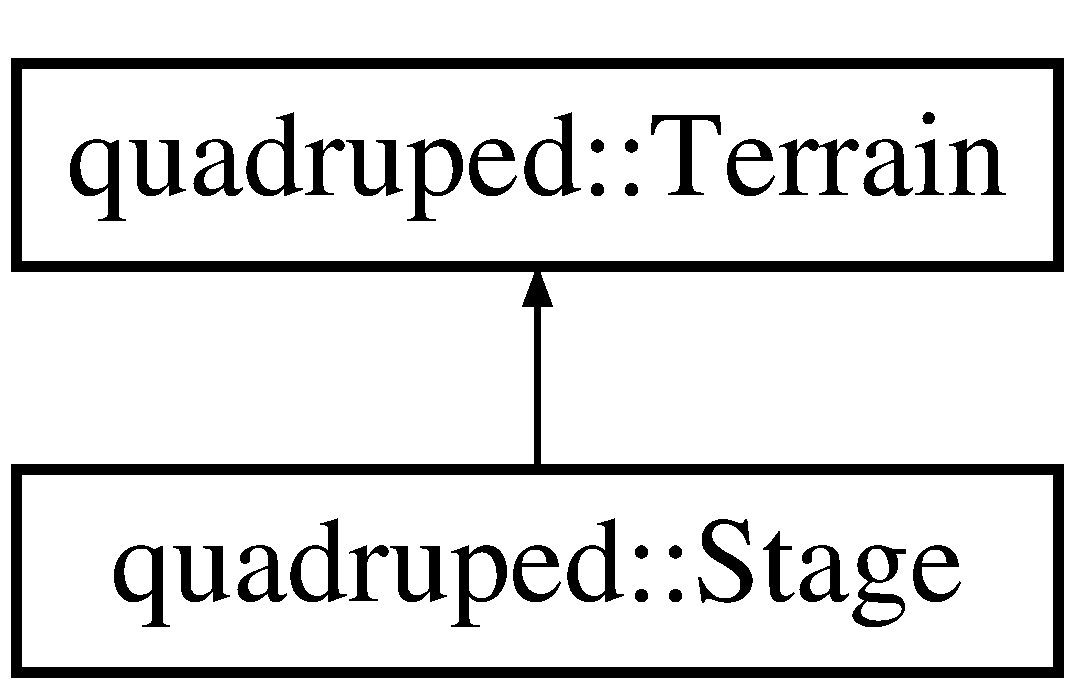
\includegraphics[height=2.000000cm]{classquadruped_1_1Stage}
\end{center}
\end{figure}
\subsection*{Public 成员函数}
\begin{DoxyCompactItemize}
\item 
\mbox{\Hypertarget{classquadruped_1_1Stage_aac6fdc1eea4355b6bcd94ef3a968895e}\label{classquadruped_1_1Stage_aac6fdc1eea4355b6bcd94ef3a968895e}} 
\hyperlink{classquadruped_1_1Stage_aac6fdc1eea4355b6bcd94ef3a968895e}{Stage} (void)
\begin{DoxyCompactList}\small\item\em Stage类的构造函数，完成地形标识符以及地形分割线的初始化 \end{DoxyCompactList}\item 
virtual double \hyperlink{classquadruped_1_1Stage_a57211e7a49be8e5413b4edb9e5051547}{Get\+Hight} (double p\+\_\+x, double p\+\_\+y) override
\begin{DoxyCompactList}\small\item\em 获取当前地形在世界坐标系下的高度 \end{DoxyCompactList}\item 
virtual void \hyperlink{classquadruped_1_1Stage_ad4e6f5c9b83346f867d0b1eb470342f3}{Updata\+Edge} (double p\+\_\+first\+\_\+edge\+\_\+\+D\+\_\+x, double p\+\_\+first\+\_\+edge\+\_\+\+D\+\_\+y) override
\begin{DoxyCompactList}\small\item\em 获取平台与地面的交线中点在世界坐标系下的位置以及分割线和危险区的设置 \end{DoxyCompactList}\item 
virtual \hyperlink{cppTypes_8h_a65c27bf97693676535dd0b30ea0ad399}{Vec3}$<$ double $>$ \hyperlink{classquadruped_1_1Stage_aefa2ad3075cce6c230b9a2c3a7de9079}{Get\+Normal\+Vector} (double p\+\_\+x, double p\+\_\+y) override
\begin{DoxyCompactList}\small\item\em 预留接口 $\vert$ 获取平台某一点处的法向量 \end{DoxyCompactList}\end{DoxyCompactItemize}
\subsection*{额外继承的成员函数}


\subsection{详细描述}
平台类子类 

\subsection{成员函数说明}
\mbox{\Hypertarget{classquadruped_1_1Stage_a57211e7a49be8e5413b4edb9e5051547}\label{classquadruped_1_1Stage_a57211e7a49be8e5413b4edb9e5051547}} 
\index{quadruped\+::\+Stage@{quadruped\+::\+Stage}!Get\+Hight@{Get\+Hight}}
\index{Get\+Hight@{Get\+Hight}!quadruped\+::\+Stage@{quadruped\+::\+Stage}}
\subsubsection{\texorpdfstring{Get\+Hight()}{GetHight()}}
{\footnotesize\ttfamily double Stage\+::\+Get\+Hight (\begin{DoxyParamCaption}\item[{double}]{p\+\_\+x,  }\item[{double}]{p\+\_\+y }\end{DoxyParamCaption})\hspace{0.3cm}{\ttfamily [override]}, {\ttfamily [virtual]}}



获取当前地形在世界坐标系下的高度 


\begin{DoxyParams}{参数}
{\em p\+\_\+x} & 当前点在世界坐标系位置坐标的\+X值 \\
\hline
{\em p\+\_\+y} & 当前点在世界坐标系位置坐标的\+Y值 \\
\hline
\end{DoxyParams}
\begin{DoxyReturn}{返回}
double 
\end{DoxyReturn}


重载 \hyperlink{classquadruped_1_1Terrain}{quadruped\+::\+Terrain} .



参考 quadruped\+::\+Terrain\+::first\+\_\+edge\+\_\+\+D\+\_\+x, S\+T\+A\+G\+E\+\_\+\+H\+E\+I\+G\+HT , 以及 S\+T\+A\+G\+E\+\_\+\+L\+E\+N\+G\+TH.

\mbox{\Hypertarget{classquadruped_1_1Stage_aefa2ad3075cce6c230b9a2c3a7de9079}\label{classquadruped_1_1Stage_aefa2ad3075cce6c230b9a2c3a7de9079}} 
\index{quadruped\+::\+Stage@{quadruped\+::\+Stage}!Get\+Normal\+Vector@{Get\+Normal\+Vector}}
\index{Get\+Normal\+Vector@{Get\+Normal\+Vector}!quadruped\+::\+Stage@{quadruped\+::\+Stage}}
\subsubsection{\texorpdfstring{Get\+Normal\+Vector()}{GetNormalVector()}}
{\footnotesize\ttfamily \hyperlink{cppTypes_8h_a65c27bf97693676535dd0b30ea0ad399}{Vec3}$<$ double $>$ Stage\+::\+Get\+Normal\+Vector (\begin{DoxyParamCaption}\item[{double}]{p\+\_\+x,  }\item[{double}]{p\+\_\+y }\end{DoxyParamCaption})\hspace{0.3cm}{\ttfamily [override]}, {\ttfamily [virtual]}}



预留接口 $\vert$ 获取平台某一点处的法向量 


\begin{DoxyParams}{参数}
{\em p\+\_\+x} & \\
\hline
{\em p\+\_\+y} & \\
\hline
\end{DoxyParams}
\begin{DoxyReturn}{返回}
Vec3$<$double$>$ 
\end{DoxyReturn}


实现了 \hyperlink{classquadruped_1_1Terrain}{quadruped\+::\+Terrain}.

\mbox{\Hypertarget{classquadruped_1_1Stage_ad4e6f5c9b83346f867d0b1eb470342f3}\label{classquadruped_1_1Stage_ad4e6f5c9b83346f867d0b1eb470342f3}} 
\index{quadruped\+::\+Stage@{quadruped\+::\+Stage}!Updata\+Edge@{Updata\+Edge}}
\index{Updata\+Edge@{Updata\+Edge}!quadruped\+::\+Stage@{quadruped\+::\+Stage}}
\subsubsection{\texorpdfstring{Updata\+Edge()}{UpdataEdge()}}
{\footnotesize\ttfamily void Stage\+::\+Updata\+Edge (\begin{DoxyParamCaption}\item[{double}]{p\+\_\+first\+\_\+edge\+\_\+\+D\+\_\+x,  }\item[{double}]{p\+\_\+first\+\_\+edge\+\_\+\+D\+\_\+y }\end{DoxyParamCaption})\hspace{0.3cm}{\ttfamily [override]}, {\ttfamily [virtual]}}



获取平台与地面的交线中点在世界坐标系下的位置以及分割线和危险区的设置 


\begin{DoxyParams}{参数}
{\em p\+\_\+first\+\_\+edge\+\_\+\+D\+\_\+x} & 当前点在世界坐标系位置坐标的\+X值 \\
\hline
{\em p\+\_\+first\+\_\+edge\+\_\+\+D\+\_\+y} & 当前点在世界坐标系位置坐标的\+Y值 \\
\hline
\end{DoxyParams}


重载 \hyperlink{classquadruped_1_1Terrain}{quadruped\+::\+Terrain} .



参考 quadruped\+::\+Terrain\+::average\+Danger\+Area, quadruped\+::\+Terrain\+::first\+\_\+edge\+\_\+\+D\+\_\+x, quadruped\+::\+Terrain\+::first\+\_\+edge\+\_\+\+D\+\_\+y, L\+I\+M\+I\+T\+\_\+\+I\+N\+F\+I\+N\+I\+TE, quadruped\+::\+Terrain\+::num\+Split, quadruped\+::\+Terrain\+::safe\+Area, quadruped\+::\+Terrain\+::split, S\+T\+A\+G\+E\+\_\+\+H\+E\+I\+G\+HT , 以及 S\+T\+A\+G\+E\+\_\+\+L\+E\+N\+G\+TH.



该类的文档由以下文件生成\+:\begin{DoxyCompactItemize}
\item 
controller/motion\+Plan/terrain/\hyperlink{terrain_8hpp}{terrain.\+hpp}\item 
controller/motion\+Plan/terrain/\hyperlink{terrain_8cpp}{terrain.\+cpp}\end{DoxyCompactItemize}

\hypertarget{classquadruped_1_1Stairs}{}\section{quadruped\+:\+:Stairs类 参考}
\label{classquadruped_1_1Stairs}\index{quadruped\+::\+Stairs@{quadruped\+::\+Stairs}}


阶梯类子类  




{\ttfamily \#include $<$terrain.\+hpp$>$}

类 quadruped\+:\+:Stairs 继承关系图\+:\begin{figure}[H]
\begin{center}
\leavevmode
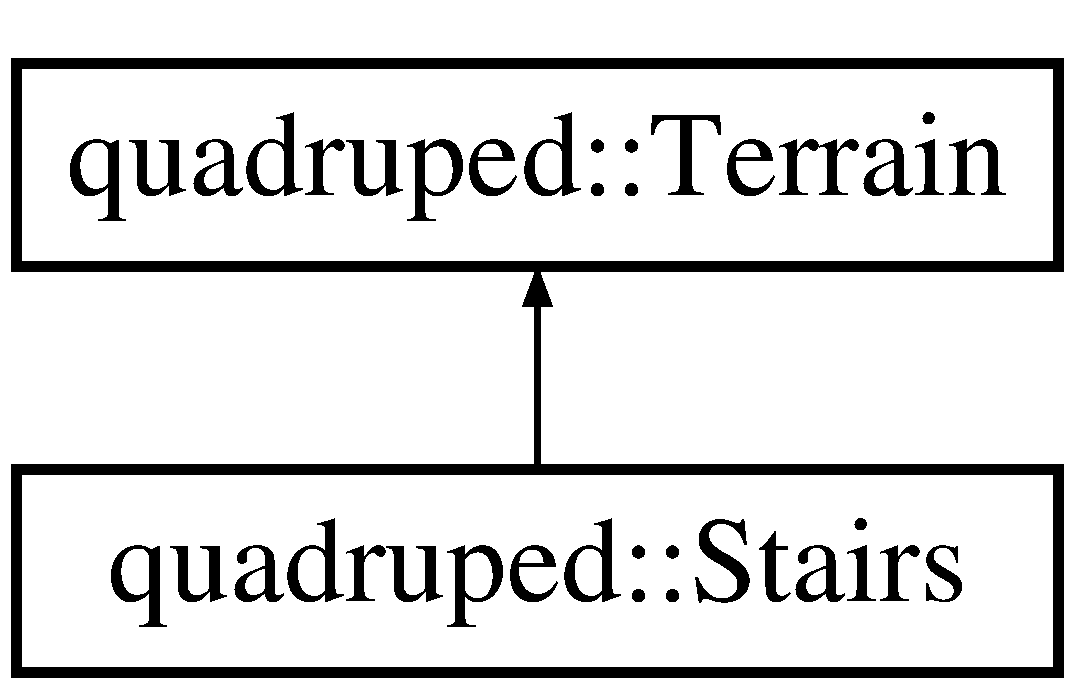
\includegraphics[height=2.000000cm]{classquadruped_1_1Stairs}
\end{center}
\end{figure}
\subsection*{Public 成员函数}
\begin{DoxyCompactItemize}
\item 
\mbox{\Hypertarget{classquadruped_1_1Stairs_a8465bdf8217036f4c3a50c52270b0d7c}\label{classquadruped_1_1Stairs_a8465bdf8217036f4c3a50c52270b0d7c}} 
\hyperlink{classquadruped_1_1Stairs_a8465bdf8217036f4c3a50c52270b0d7c}{Stairs} (void)
\begin{DoxyCompactList}\small\item\em Stairs类的构造函数，完成地形标识符以及地形分割线的初始化 \end{DoxyCompactList}\item 
virtual double \hyperlink{classquadruped_1_1Stairs_a648ed016d7ba3648e27ecd7eecdb3ab2}{Get\+Hight} (double p\+\_\+x, double p\+\_\+y) override
\begin{DoxyCompactList}\small\item\em 获取当前地形在世界坐标系下的高度 \end{DoxyCompactList}\item 
virtual void \hyperlink{classquadruped_1_1Stairs_a37a4cc06123b8eba97a05049e8a5fcd0}{Updata\+Edge} (double p\+\_\+first\+\_\+edge\+\_\+\+D\+\_\+x, double p\+\_\+first\+\_\+edge\+\_\+\+D\+\_\+y) override
\begin{DoxyCompactList}\small\item\em 获取阶梯与地面的交线中点在世界坐标系下的位置以及分割线和危险区的设置 \end{DoxyCompactList}\item 
virtual \hyperlink{cppTypes_8h_a65c27bf97693676535dd0b30ea0ad399}{Vec3}$<$ double $>$ \hyperlink{classquadruped_1_1Stairs_ac14852afde37318cf3390c4090a991f1}{Get\+Normal\+Vector} (double p\+\_\+x, double p\+\_\+y) override
\begin{DoxyCompactList}\small\item\em 预留接口 $\vert$ 获取阶梯某一点处的法向量 \end{DoxyCompactList}\end{DoxyCompactItemize}
\subsection*{额外继承的成员函数}


\subsection{详细描述}
阶梯类子类 

\subsection{成员函数说明}
\mbox{\Hypertarget{classquadruped_1_1Stairs_a648ed016d7ba3648e27ecd7eecdb3ab2}\label{classquadruped_1_1Stairs_a648ed016d7ba3648e27ecd7eecdb3ab2}} 
\index{quadruped\+::\+Stairs@{quadruped\+::\+Stairs}!Get\+Hight@{Get\+Hight}}
\index{Get\+Hight@{Get\+Hight}!quadruped\+::\+Stairs@{quadruped\+::\+Stairs}}
\subsubsection{\texorpdfstring{Get\+Hight()}{GetHight()}}
{\footnotesize\ttfamily double Stairs\+::\+Get\+Hight (\begin{DoxyParamCaption}\item[{double}]{p\+\_\+x,  }\item[{double}]{p\+\_\+y }\end{DoxyParamCaption})\hspace{0.3cm}{\ttfamily [override]}, {\ttfamily [virtual]}}



获取当前地形在世界坐标系下的高度 


\begin{DoxyParams}{参数}
{\em p\+\_\+x} & 当前点在世界坐标系位置坐标的\+X值 \\
\hline
{\em p\+\_\+y} & 当前点在世界坐标系位置坐标的\+Y值 \\
\hline
\end{DoxyParams}
\begin{DoxyReturn}{返回}
double 
\end{DoxyReturn}


重载 \hyperlink{classquadruped_1_1Terrain}{quadruped\+::\+Terrain} .



参考 quadruped\+::\+Terrain\+::first\+\_\+edge\+\_\+\+D\+\_\+x, S\+T\+A\+I\+R\+S\+\_\+\+D\+E\+P\+TH , 以及 S\+T\+A\+I\+R\+S\+\_\+\+H\+E\+I\+G\+HT.

\mbox{\Hypertarget{classquadruped_1_1Stairs_ac14852afde37318cf3390c4090a991f1}\label{classquadruped_1_1Stairs_ac14852afde37318cf3390c4090a991f1}} 
\index{quadruped\+::\+Stairs@{quadruped\+::\+Stairs}!Get\+Normal\+Vector@{Get\+Normal\+Vector}}
\index{Get\+Normal\+Vector@{Get\+Normal\+Vector}!quadruped\+::\+Stairs@{quadruped\+::\+Stairs}}
\subsubsection{\texorpdfstring{Get\+Normal\+Vector()}{GetNormalVector()}}
{\footnotesize\ttfamily \hyperlink{cppTypes_8h_a65c27bf97693676535dd0b30ea0ad399}{Vec3}$<$ double $>$ Stairs\+::\+Get\+Normal\+Vector (\begin{DoxyParamCaption}\item[{double}]{p\+\_\+x,  }\item[{double}]{p\+\_\+y }\end{DoxyParamCaption})\hspace{0.3cm}{\ttfamily [override]}, {\ttfamily [virtual]}}



预留接口 $\vert$ 获取阶梯某一点处的法向量 


\begin{DoxyParams}{参数}
{\em p\+\_\+x} & \\
\hline
{\em p\+\_\+y} & \\
\hline
\end{DoxyParams}
\begin{DoxyReturn}{返回}
Vec3$<$double$>$ 
\end{DoxyReturn}


实现了 \hyperlink{classquadruped_1_1Terrain}{quadruped\+::\+Terrain}.

\mbox{\Hypertarget{classquadruped_1_1Stairs_a37a4cc06123b8eba97a05049e8a5fcd0}\label{classquadruped_1_1Stairs_a37a4cc06123b8eba97a05049e8a5fcd0}} 
\index{quadruped\+::\+Stairs@{quadruped\+::\+Stairs}!Updata\+Edge@{Updata\+Edge}}
\index{Updata\+Edge@{Updata\+Edge}!quadruped\+::\+Stairs@{quadruped\+::\+Stairs}}
\subsubsection{\texorpdfstring{Updata\+Edge()}{UpdataEdge()}}
{\footnotesize\ttfamily void Stairs\+::\+Updata\+Edge (\begin{DoxyParamCaption}\item[{double}]{p\+\_\+first\+\_\+edge\+\_\+\+D\+\_\+x,  }\item[{double}]{p\+\_\+first\+\_\+edge\+\_\+\+D\+\_\+y }\end{DoxyParamCaption})\hspace{0.3cm}{\ttfamily [override]}, {\ttfamily [virtual]}}



获取阶梯与地面的交线中点在世界坐标系下的位置以及分割线和危险区的设置 


\begin{DoxyParams}{参数}
{\em p\+\_\+first\+\_\+edge\+\_\+\+D\+\_\+x} & 当前点在世界坐标系位置坐标的\+X值 \\
\hline
{\em p\+\_\+first\+\_\+edge\+\_\+\+D\+\_\+y} & 当前点在世界坐标系位置坐标的\+Y值 \\
\hline
\end{DoxyParams}


重载 \hyperlink{classquadruped_1_1Terrain}{quadruped\+::\+Terrain} .



参考 quadruped\+::\+Terrain\+::average\+Danger\+Area, quadruped\+::\+Terrain\+::first\+\_\+edge\+\_\+\+D\+\_\+x, quadruped\+::\+Terrain\+::first\+\_\+edge\+\_\+\+D\+\_\+y, L\+I\+M\+I\+T\+\_\+\+I\+N\+F\+I\+N\+I\+TE, quadruped\+::\+Terrain\+::num\+Split, quadruped\+::\+Terrain\+::safe\+Area, quadruped\+::\+Terrain\+::split, S\+T\+A\+I\+R\+S\+\_\+\+D\+E\+P\+TH , 以及 S\+T\+A\+I\+R\+S\+\_\+\+H\+E\+I\+G\+HT.



该类的文档由以下文件生成\+:\begin{DoxyCompactItemize}
\item 
controller/motion\+Plan/terrain/\hyperlink{terrain_8hpp}{terrain.\+hpp}\item 
controller/motion\+Plan/terrain/\hyperlink{terrain_8cpp}{terrain.\+cpp}\end{DoxyCompactItemize}

\hypertarget{classquadruped_1_1StateMachine}{}\section{quadruped\+:\+:State\+Machine类 参考}
\label{classquadruped_1_1StateMachine}\index{quadruped\+::\+State\+Machine@{quadruped\+::\+State\+Machine}}
\subsection*{Public 属性}
\begin{DoxyCompactItemize}
\item 
\mbox{\Hypertarget{classquadruped_1_1StateMachine_a105927d0ab33d29e72f2ee6a67dffe85}\label{classquadruped_1_1StateMachine_a105927d0ab33d29e72f2ee6a67dffe85}} 
uint32\+\_\+t {\bfseries period} = 200
\item 
\mbox{\Hypertarget{classquadruped_1_1StateMachine_a25577b87297698e036afffa90d8cef06}\label{classquadruped_1_1StateMachine_a25577b87297698e036afffa90d8cef06}} 
uint32\+\_\+t {\bfseries stance\+Time} = 0
\end{DoxyCompactItemize}


该类的文档由以下文件生成\+:\begin{DoxyCompactItemize}
\item 
controller/motion\+Plan/state\+Machine.\+hpp\item 
controller/motion\+Plan/\hyperlink{stateMachine_8cpp}{state\+Machine.\+cpp}\end{DoxyCompactItemize}

\hypertarget{classquadruped_1_1Task}{}\section{quadruped\+:\+:Task类 参考}
\label{classquadruped_1_1Task}\index{quadruped\+::\+Task@{quadruped\+::\+Task}}
类 quadruped\+:\+:Task 继承关系图\+:\begin{figure}[H]
\begin{center}
\leavevmode
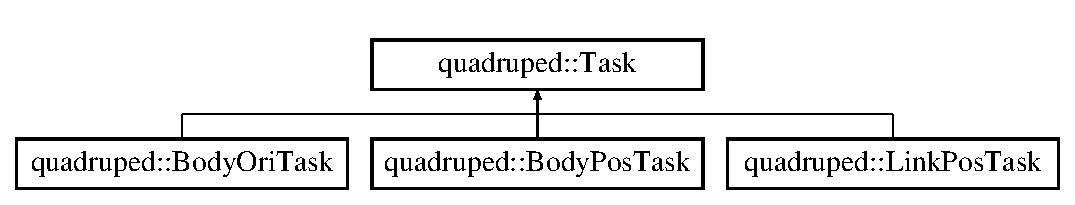
\includegraphics[height=2.000000cm]{classquadruped_1_1Task}
\end{center}
\end{figure}
\subsection*{Public 成员函数}
\begin{DoxyCompactItemize}
\item 
\mbox{\Hypertarget{classquadruped_1_1Task_a613c1f3369686563c55aff12749f319e}\label{classquadruped_1_1Task_a613c1f3369686563c55aff12749f319e}} 
{\bfseries Task} (size\+\_\+t dim)
\item 
\mbox{\Hypertarget{classquadruped_1_1Task_a6e083e753f2f0d6c7cbcb1cbfc21c561}\label{classquadruped_1_1Task_a6e083e753f2f0d6c7cbcb1cbfc21c561}} 
void {\bfseries Get\+Command} (\hyperlink{cppTypes_8h_adad69baca3c77d5f991be5d3c063fea7}{D\+Vec}$<$ double $>$ \&p\+\_\+acc\+\_\+cmd)
\item 
\mbox{\Hypertarget{classquadruped_1_1Task_a0215eff9e1ee48600e3c74c177fbebb8}\label{classquadruped_1_1Task_a0215eff9e1ee48600e3c74c177fbebb8}} 
void {\bfseries Get\+Task\+Jacobian} (\hyperlink{cppTypes_8h_a5db6bfb25afa103db1fb6bb6287ae9d7}{D\+Mat}$<$ double $>$ \&p\+\_\+\+Jt)
\item 
\mbox{\Hypertarget{classquadruped_1_1Task_a03389dcd6fa90066f8fdf295263f5eb1}\label{classquadruped_1_1Task_a03389dcd6fa90066f8fdf295263f5eb1}} 
void {\bfseries Get\+Task\+Jacobian\+Dot\+Qdot} (\hyperlink{cppTypes_8h_adad69baca3c77d5f991be5d3c063fea7}{D\+Vec}$<$ double $>$ \&p\+\_\+\+Jt\+Dot\+Qdot)
\item 
\mbox{\Hypertarget{classquadruped_1_1Task_a7124a97e1f935fc9c4faf66284c06343}\label{classquadruped_1_1Task_a7124a97e1f935fc9c4faf66284c06343}} 
bool {\bfseries Update\+Task} (const \hyperlink{cppTypes_8h_adad69baca3c77d5f991be5d3c063fea7}{D\+Vec}$<$ double $>$ \&p\+\_\+pos\+\_\+des, const \hyperlink{cppTypes_8h_adad69baca3c77d5f991be5d3c063fea7}{D\+Vec}$<$ double $>$ \&p\+\_\+vel\+\_\+des, const \hyperlink{cppTypes_8h_adad69baca3c77d5f991be5d3c063fea7}{D\+Vec}$<$ double $>$ \&p\+\_\+acc\+\_\+des)
\item 
\mbox{\Hypertarget{classquadruped_1_1Task_a6a3beb33871582c7ca9e9df169e0bd7d}\label{classquadruped_1_1Task_a6a3beb33871582c7ca9e9df169e0bd7d}} 
bool {\bfseries Is\+Task\+Set} ()
\item 
\mbox{\Hypertarget{classquadruped_1_1Task_a1cb8eace23a5221ad65c9d89cb7d679e}\label{classquadruped_1_1Task_a1cb8eace23a5221ad65c9d89cb7d679e}} 
size\+\_\+t {\bfseries Get\+Dim} ()
\item 
\mbox{\Hypertarget{classquadruped_1_1Task_a76f4fc058fcc5300d1cb894656ffb180}\label{classquadruped_1_1Task_a76f4fc058fcc5300d1cb894656ffb180}} 
void {\bfseries Unset\+Task} ()
\item 
\mbox{\Hypertarget{classquadruped_1_1Task_a8728dd3f97ef1119690bf1497d7210ad}\label{classquadruped_1_1Task_a8728dd3f97ef1119690bf1497d7210ad}} 
const \hyperlink{cppTypes_8h_adad69baca3c77d5f991be5d3c063fea7}{D\+Vec}$<$ double $>$ \& {\bfseries Get\+Pos\+Error} ()
\item 
\mbox{\Hypertarget{classquadruped_1_1Task_a3ea78c46b815e0761f39aae7863c4ec0}\label{classquadruped_1_1Task_a3ea78c46b815e0761f39aae7863c4ec0}} 
const \hyperlink{cppTypes_8h_adad69baca3c77d5f991be5d3c063fea7}{D\+Vec}$<$ double $>$ \& {\bfseries Get\+Des\+Vel} ()
\item 
\mbox{\Hypertarget{classquadruped_1_1Task_a7ec90dfce229f16c453f2b7d5c930a41}\label{classquadruped_1_1Task_a7ec90dfce229f16c453f2b7d5c930a41}} 
const \hyperlink{cppTypes_8h_adad69baca3c77d5f991be5d3c063fea7}{D\+Vec}$<$ double $>$ \& {\bfseries Get\+Des\+Acc} ()
\end{DoxyCompactItemize}
\subsection*{Protected 成员函数}
\begin{DoxyCompactItemize}
\item 
\mbox{\Hypertarget{classquadruped_1_1Task_ae35ff689655939445b43f819539b028d}\label{classquadruped_1_1Task_ae35ff689655939445b43f819539b028d}} 
virtual bool {\bfseries Update\+Command} (const \hyperlink{cppTypes_8h_adad69baca3c77d5f991be5d3c063fea7}{D\+Vec}$<$ double $>$ \&p\+\_\+pos\+\_\+des, const \hyperlink{cppTypes_8h_adad69baca3c77d5f991be5d3c063fea7}{D\+Vec}$<$ double $>$ \&p\+\_\+vel\+\_\+des, const \hyperlink{cppTypes_8h_adad69baca3c77d5f991be5d3c063fea7}{D\+Vec}$<$ double $>$ \&p\+\_\+acc\+\_\+des)=0
\item 
\mbox{\Hypertarget{classquadruped_1_1Task_adcb39e5aa2daffbb72baabad7a414ae2}\label{classquadruped_1_1Task_adcb39e5aa2daffbb72baabad7a414ae2}} 
virtual bool {\bfseries Update\+Task\+Jacobian} ()=0
\item 
\mbox{\Hypertarget{classquadruped_1_1Task_ae818a2d7e013929563a859144cf050bb}\label{classquadruped_1_1Task_ae818a2d7e013929563a859144cf050bb}} 
virtual bool {\bfseries Update\+Task\+J\+Dot\+Qdot} ()=0
\item 
\mbox{\Hypertarget{classquadruped_1_1Task_aa6e18f427f6a31fb9a5d9267cc707550}\label{classquadruped_1_1Task_aa6e18f427f6a31fb9a5d9267cc707550}} 
virtual bool {\bfseries Additional\+Update} ()=0
\end{DoxyCompactItemize}
\subsection*{Protected 属性}
\begin{DoxyCompactItemize}
\item 
\mbox{\Hypertarget{classquadruped_1_1Task_a70287d1a65e0ea275c1495776e6a4b98}\label{classquadruped_1_1Task_a70287d1a65e0ea275c1495776e6a4b98}} 
bool {\bfseries b\+\_\+set\+\_\+task}
\item 
\mbox{\Hypertarget{classquadruped_1_1Task_a6e52946ddee1c043fd46c8e0369caed1}\label{classquadruped_1_1Task_a6e52946ddee1c043fd46c8e0369caed1}} 
size\+\_\+t {\bfseries dim\+\_\+task}
\item 
\mbox{\Hypertarget{classquadruped_1_1Task_adee90b42eaf44c394939a2a60f3abb47}\label{classquadruped_1_1Task_adee90b42eaf44c394939a2a60f3abb47}} 
\hyperlink{cppTypes_8h_adad69baca3c77d5f991be5d3c063fea7}{D\+Vec}$<$ double $>$ {\bfseries acc\+\_\+cmd}
\item 
\mbox{\Hypertarget{classquadruped_1_1Task_afd7cdc7374425c08638589b6d0628344}\label{classquadruped_1_1Task_afd7cdc7374425c08638589b6d0628344}} 
\hyperlink{cppTypes_8h_adad69baca3c77d5f991be5d3c063fea7}{D\+Vec}$<$ double $>$ {\bfseries Jt\+Dot\+Qdot}
\item 
\mbox{\Hypertarget{classquadruped_1_1Task_a5127c2483fca6045c7636dc70ecea8c5}\label{classquadruped_1_1Task_a5127c2483fca6045c7636dc70ecea8c5}} 
\hyperlink{cppTypes_8h_a5db6bfb25afa103db1fb6bb6287ae9d7}{D\+Mat}$<$ double $>$ {\bfseries Jt}
\item 
\mbox{\Hypertarget{classquadruped_1_1Task_a4a3561457b67406e2801a5f9d73ca3e7}\label{classquadruped_1_1Task_a4a3561457b67406e2801a5f9d73ca3e7}} 
\hyperlink{cppTypes_8h_adad69baca3c77d5f991be5d3c063fea7}{D\+Vec}$<$ double $>$ {\bfseries pos\+\_\+err}
\item 
\mbox{\Hypertarget{classquadruped_1_1Task_ac750af3351815900cc14bbdee1925ef7}\label{classquadruped_1_1Task_ac750af3351815900cc14bbdee1925ef7}} 
\hyperlink{cppTypes_8h_adad69baca3c77d5f991be5d3c063fea7}{D\+Vec}$<$ double $>$ {\bfseries vel\+\_\+des}
\item 
\mbox{\Hypertarget{classquadruped_1_1Task_a73d69db6f8d512b10e00a99a77d38b48}\label{classquadruped_1_1Task_a73d69db6f8d512b10e00a99a77d38b48}} 
\hyperlink{cppTypes_8h_adad69baca3c77d5f991be5d3c063fea7}{D\+Vec}$<$ double $>$ {\bfseries acc\+\_\+des}
\end{DoxyCompactItemize}


该类的文档由以下文件生成\+:\begin{DoxyCompactItemize}
\item 
controller/wbc/task\+Set/task.\+hpp\end{DoxyCompactItemize}

\hypertarget{classquadruped_1_1Terrain}{}\section{quadruped\+:\+:Terrain类 参考}
\label{classquadruped_1_1Terrain}\index{quadruped\+::\+Terrain@{quadruped\+::\+Terrain}}


地形类父类  




{\ttfamily \#include $<$terrain.\+hpp$>$}

类 quadruped\+:\+:Terrain 继承关系图\+:\begin{figure}[H]
\begin{center}
\leavevmode
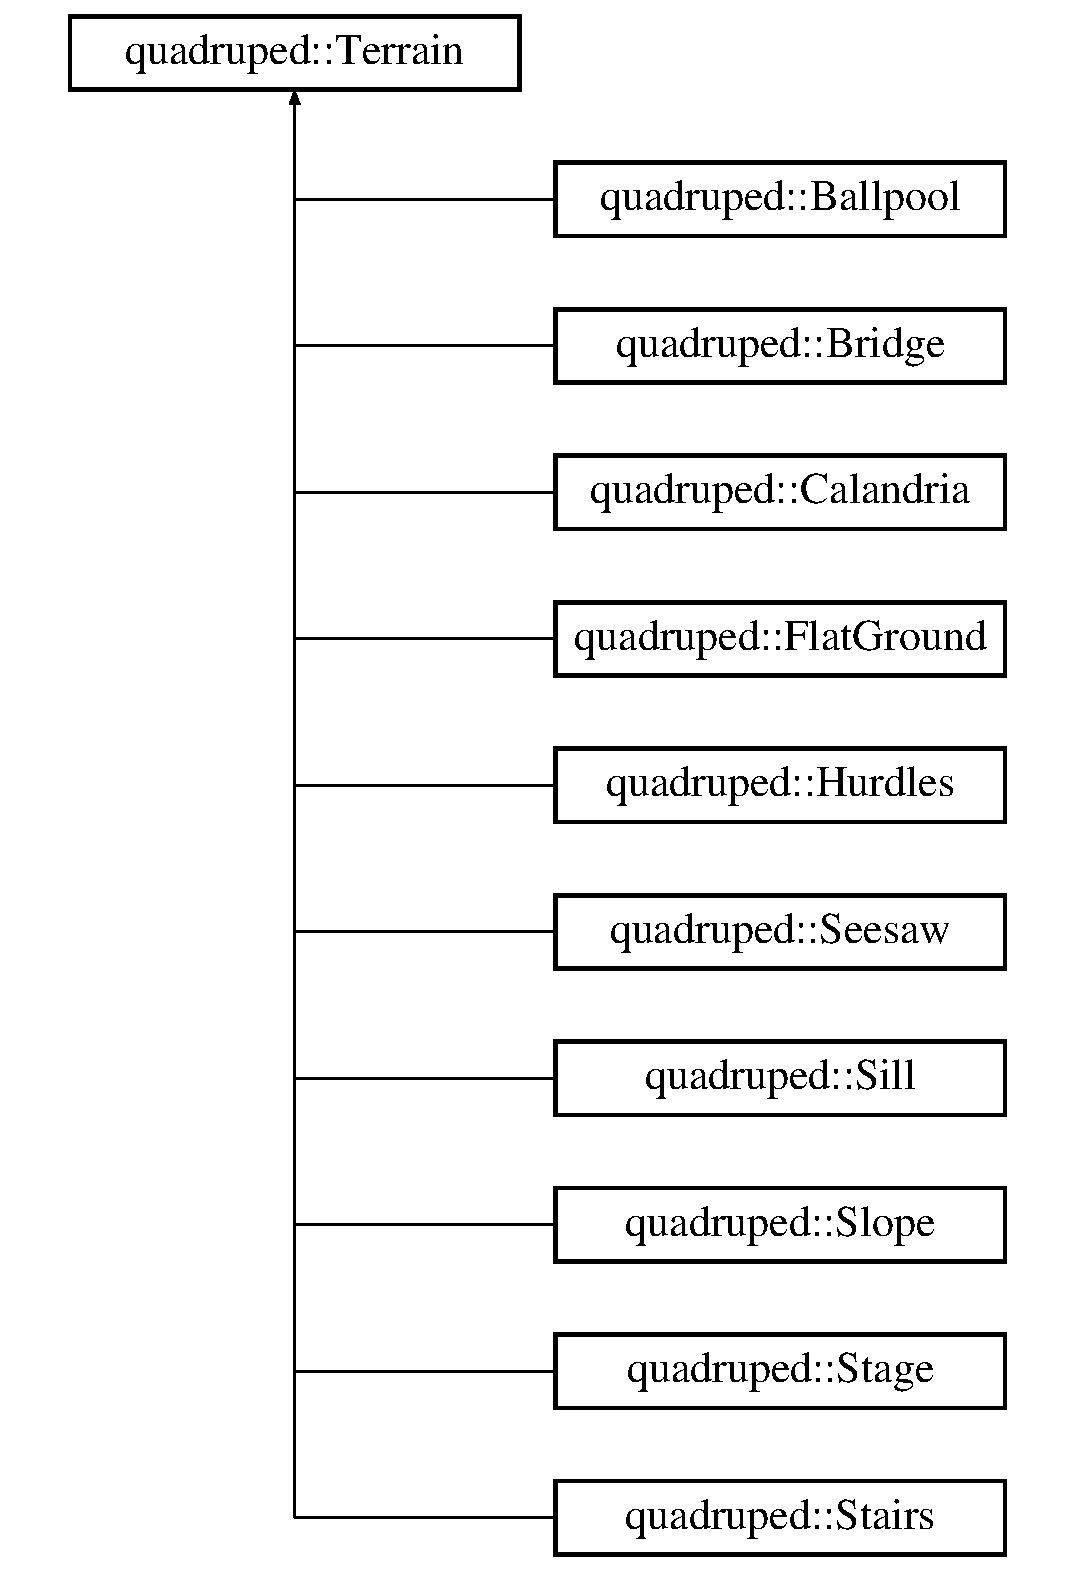
\includegraphics[height=11.000000cm]{classquadruped_1_1Terrain}
\end{center}
\end{figure}
\subsection*{Public 成员函数}
\begin{DoxyCompactItemize}
\item 
\mbox{\Hypertarget{classquadruped_1_1Terrain_a47d42e31c537473dba5c75ffae3d0159}\label{classquadruped_1_1Terrain_a47d42e31c537473dba5c75ffae3d0159}} 
\hyperlink{classquadruped_1_1Terrain_a47d42e31c537473dba5c75ffae3d0159}{Terrain} (void)
\begin{DoxyCompactList}\small\item\em 地形类的构造函数 \end{DoxyCompactList}\item 
\mbox{\Hypertarget{classquadruped_1_1Terrain_adbecae34d794bcf2c6707a695634dec9}\label{classquadruped_1_1Terrain_adbecae34d794bcf2c6707a695634dec9}} 
virtual \hyperlink{classquadruped_1_1Terrain_adbecae34d794bcf2c6707a695634dec9}{$\sim$\+Terrain} (void)
\begin{DoxyCompactList}\small\item\em 地形类的析构函数 \end{DoxyCompactList}\item 
\mbox{\Hypertarget{classquadruped_1_1Terrain_a9ba4414b8202818c5de34abde4e653e8}\label{classquadruped_1_1Terrain_a9ba4414b8202818c5de34abde4e653e8}} 
double {\bfseries Get\+Derivative\+Of\+Height\+Wrt} (Dim2D p\+\_\+dim, double p\+\_\+x, double p\+\_\+y)
\item 
\mbox{\Hypertarget{classquadruped_1_1Terrain_ac863b65b5390ffdb8c7651b0e5ffa5c5}\label{classquadruped_1_1Terrain_ac863b65b5390ffdb8c7651b0e5ffa5c5}} 
double {\bfseries Get\+Second\+Derivative\+Of\+Height\+Wrt} (Dim2D p\+\_\+dim1, Dim2D p\+\_\+dim2, double p\+\_\+x, double p\+\_\+y)
\item 
\mbox{\Hypertarget{classquadruped_1_1Terrain_a5dd93d757ea342da62c185e801ea54d6}\label{classquadruped_1_1Terrain_a5dd93d757ea342da62c185e801ea54d6}} 
virtual double {\bfseries Get\+Hight} (double p\+\_\+x, double p\+\_\+y)
\item 
\mbox{\Hypertarget{classquadruped_1_1Terrain_ae8768e1ea061d8ca892950082c7820f2}\label{classquadruped_1_1Terrain_ae8768e1ea061d8ca892950082c7820f2}} 
virtual double {\bfseries Get\+Height\+Deriv\+WrtX} (double x, double y)
\item 
\mbox{\Hypertarget{classquadruped_1_1Terrain_af7cd36d8d76d0868c07c5c620f595084}\label{classquadruped_1_1Terrain_af7cd36d8d76d0868c07c5c620f595084}} 
virtual double {\bfseries Get\+Height\+Deriv\+WrtY} (double x, double y)
\item 
\mbox{\Hypertarget{classquadruped_1_1Terrain_a568de4c587f00f23363ee45bf00f6c70}\label{classquadruped_1_1Terrain_a568de4c587f00f23363ee45bf00f6c70}} 
virtual double {\bfseries Get\+Height\+Deriv\+Wrt\+XX} (double x, double y)
\item 
\mbox{\Hypertarget{classquadruped_1_1Terrain_a0719f91623952c4edb689ba86789f443}\label{classquadruped_1_1Terrain_a0719f91623952c4edb689ba86789f443}} 
virtual double {\bfseries Get\+Height\+Deriv\+Wrt\+XY} (double x, double y)
\item 
\mbox{\Hypertarget{classquadruped_1_1Terrain_a7084e067ce0466f009ae74450a0247ed}\label{classquadruped_1_1Terrain_a7084e067ce0466f009ae74450a0247ed}} 
virtual double {\bfseries Get\+Height\+Deriv\+Wrt\+YX} (double x, double y)
\item 
\mbox{\Hypertarget{classquadruped_1_1Terrain_a8a9ef6d376b56d0f3a4a35716a553caf}\label{classquadruped_1_1Terrain_a8a9ef6d376b56d0f3a4a35716a553caf}} 
virtual double {\bfseries Get\+Height\+Deriv\+Wrt\+YY} (double x, double y)
\item 
\mbox{\Hypertarget{classquadruped_1_1Terrain_a3cf3e2e194eabcd6917b1911fe66fac2}\label{classquadruped_1_1Terrain_a3cf3e2e194eabcd6917b1911fe66fac2}} 
virtual void {\bfseries Updata\+Edge} (double p\+\_\+first\+\_\+edge\+\_\+\+D\+\_\+x, double p\+\_\+first\+\_\+edge\+\_\+\+D\+\_\+y)
\item 
\mbox{\Hypertarget{classquadruped_1_1Terrain_aa93648530b689a96eb46b37a0aa33b67}\label{classquadruped_1_1Terrain_aa93648530b689a96eb46b37a0aa33b67}} 
virtual \hyperlink{cppTypes_8h_a65c27bf97693676535dd0b30ea0ad399}{Vec3}$<$ double $>$ {\bfseries Get\+Normal\+Vector} (double p\+\_\+x, double p\+\_\+y)=0
\end{DoxyCompactItemize}
\subsection*{Public 属性}
\begin{DoxyCompactItemize}
\item 
\mbox{\Hypertarget{classquadruped_1_1Terrain_a10c9a4f5aafbf2dcc398217313102224}\label{classquadruped_1_1Terrain_a10c9a4f5aafbf2dcc398217313102224}} 
uint8\+\_\+t \hyperlink{classquadruped_1_1Terrain_a10c9a4f5aafbf2dcc398217313102224}{terrain\+\_\+id} = 0
\begin{DoxyCompactList}\small\item\em 地形标识符 \end{DoxyCompactList}\item 
\mbox{\Hypertarget{classquadruped_1_1Terrain_a920a6fe3be9b95ac56e354bb4e5652bc}\label{classquadruped_1_1Terrain_a920a6fe3be9b95ac56e354bb4e5652bc}} 
double \hyperlink{classquadruped_1_1Terrain_a920a6fe3be9b95ac56e354bb4e5652bc}{first\+\_\+edge\+\_\+\+D\+\_\+x} = 0
\begin{DoxyCompactList}\small\item\em 障碍与地面的交线中点在机体坐标系\+X方向上的位置 \end{DoxyCompactList}\item 
\mbox{\Hypertarget{classquadruped_1_1Terrain_a17d5fd7b42086c04804a8cede92b4016}\label{classquadruped_1_1Terrain_a17d5fd7b42086c04804a8cede92b4016}} 
double \hyperlink{classquadruped_1_1Terrain_a17d5fd7b42086c04804a8cede92b4016}{first\+\_\+edge\+\_\+\+D\+\_\+y} = 0
\begin{DoxyCompactList}\small\item\em 障碍与地面的交线中点在机体坐标系\+Y方向上的位置 \end{DoxyCompactList}\item 
\mbox{\Hypertarget{classquadruped_1_1Terrain_a76b27de76e92a1c6672a0250e13e4a8b}\label{classquadruped_1_1Terrain_a76b27de76e92a1c6672a0250e13e4a8b}} 
std\+::vector$<$ double $>$ \hyperlink{classquadruped_1_1Terrain_a76b27de76e92a1c6672a0250e13e4a8b}{split} = \{0.\+0 , 0.\+0 , 0.\+0 , 0.\+0 , 0.\+0 , 0.\+0\}
\begin{DoxyCompactList}\small\item\em 地形分割线，对应于障碍的棱线 \end{DoxyCompactList}\item 
std\+::vector$<$ std\+::pair$<$ double, double $>$ $>$ \hyperlink{classquadruped_1_1Terrain_a69b84f242ebea84c8ef3fba2fb6a447b}{safe\+Area}
\begin{DoxyCompactList}\small\item\em 以地形分割线为中心的安全区 \end{DoxyCompactList}\item 
\mbox{\Hypertarget{classquadruped_1_1Terrain_a59d084e80702d4b598716d67c9dd9643}\label{classquadruped_1_1Terrain_a59d084e80702d4b598716d67c9dd9643}} 
int \hyperlink{classquadruped_1_1Terrain_a59d084e80702d4b598716d67c9dd9643}{num\+Split}
\begin{DoxyCompactList}\small\item\em 地形分割线个数 \end{DoxyCompactList}\item 
\mbox{\Hypertarget{classquadruped_1_1Terrain_af7ef7ef218c95c6421b71519e50f30c0}\label{classquadruped_1_1Terrain_af7ef7ef218c95c6421b71519e50f30c0}} 
double \hyperlink{classquadruped_1_1Terrain_af7ef7ef218c95c6421b71519e50f30c0}{average\+Danger\+Area}
\begin{DoxyCompactList}\small\item\em 平均危险区 \end{DoxyCompactList}\end{DoxyCompactItemize}


\subsection{详细描述}
地形类父类 

\subsection{类成员变量说明}
\mbox{\Hypertarget{classquadruped_1_1Terrain_a69b84f242ebea84c8ef3fba2fb6a447b}\label{classquadruped_1_1Terrain_a69b84f242ebea84c8ef3fba2fb6a447b}} 
\index{quadruped\+::\+Terrain@{quadruped\+::\+Terrain}!safe\+Area@{safe\+Area}}
\index{safe\+Area@{safe\+Area}!quadruped\+::\+Terrain@{quadruped\+::\+Terrain}}
\subsubsection{\texorpdfstring{safe\+Area}{safeArea}}
{\footnotesize\ttfamily std\+::vector$<$std\+::pair$<$double,double$>$ $>$ quadruped\+::\+Terrain\+::safe\+Area}

{\bfseries 初始值\+:}
\begin{DoxyCode}
= \{\{0.0 , \hyperlink{commonFunction_8hpp_a0da379bb50439fd7530cd70c59cdd8ba}{LIMIT\_INFINITE}\} , 
                                                          \{0.0 , \hyperlink{commonFunction_8hpp_a0da379bb50439fd7530cd70c59cdd8ba}{LIMIT\_INFINITE}\} ,
                                                          \{0.0 , \hyperlink{commonFunction_8hpp_a0da379bb50439fd7530cd70c59cdd8ba}{LIMIT\_INFINITE}\} ,
                                                          \{0.0 , \hyperlink{commonFunction_8hpp_a0da379bb50439fd7530cd70c59cdd8ba}{LIMIT\_INFINITE}\} ,
                                                          \{0.0 , \hyperlink{commonFunction_8hpp_a0da379bb50439fd7530cd70c59cdd8ba}{LIMIT\_INFINITE}\} ,
                                                          \{0.0 , \hyperlink{commonFunction_8hpp_a0da379bb50439fd7530cd70c59cdd8ba}{LIMIT\_INFINITE}\} \}
\end{DoxyCode}


以地形分割线为中心的安全区 



参考自 quadruped\+::\+F\+H\+\_\+constraints\+::\+Get\+Other\+Cst(), quadruped\+::\+F\+H\+\_\+constraints\+::\+Get\+Other\+Cst\+Bound(), quadruped\+::\+Stage\+::\+Updata\+Edge(), quadruped\+::\+Sill\+::\+Updata\+Edge(), quadruped\+::\+Calandria\+::\+Updata\+Edge(), quadruped\+::\+Stairs\+::\+Updata\+Edge() , 以及 quadruped\+::\+Bridge\+::\+Updata\+Edge().



该类的文档由以下文件生成\+:\begin{DoxyCompactItemize}
\item 
controller/motion\+Plan/terrain/\hyperlink{terrain_8hpp}{terrain.\+hpp}\item 
controller/motion\+Plan/terrain/\hyperlink{terrain_8cpp}{terrain.\+cpp}\end{DoxyCompactItemize}

\hypertarget{classVelocityEstimate}{}\section{Velocity\+Estimate类 参考}
\label{classVelocityEstimate}\index{Velocity\+Estimate@{Velocity\+Estimate}}
\subsection*{Public 成员函数}
\begin{DoxyCompactItemize}
\item 
\mbox{\Hypertarget{classVelocityEstimate_a9cf353e393f834f1ee1fcd27871b662f}\label{classVelocityEstimate_a9cf353e393f834f1ee1fcd27871b662f}} 
void {\bfseries vector2crossmatrix} (const \hyperlink{cppTypes_8h_a65c27bf97693676535dd0b30ea0ad399}{Vec3}$<$ double $>$ \&vector\+\_\+input, \hyperlink{cppTypes_8h_adb7d462b35d31f0b2583b3e230a2a2c3}{Mat3}$<$ double $>$ \&matrix\+\_\+input)
\item 
\mbox{\Hypertarget{classVelocityEstimate_a008b3eb136ed2006728593d972aa186c}\label{classVelocityEstimate_a008b3eb136ed2006728593d972aa186c}} 
\hyperlink{cppTypes_8h_a65c27bf97693676535dd0b30ea0ad399}{Vec3}$<$ double $>$ {\bfseries Cal\+Velocity} (bool L\+F\+\_\+\+C\+O\+N\+T\+A\+CT, bool L\+R\+\_\+\+C\+O\+N\+T\+A\+CT, bool R\+F\+\_\+\+C\+O\+N\+T\+A\+CT, bool R\+R\+\_\+\+C\+O\+N\+T\+A\+CT, \hyperlink{cppTypes_8h_a65c27bf97693676535dd0b30ea0ad399}{Vec3}$<$ double $>$ lf\+\_\+endfoot\+\_\+vel, \hyperlink{cppTypes_8h_a65c27bf97693676535dd0b30ea0ad399}{Vec3}$<$ double $>$ lr\+\_\+endfoot\+\_\+vel, \hyperlink{cppTypes_8h_a65c27bf97693676535dd0b30ea0ad399}{Vec3}$<$ double $>$ rf\+\_\+endfoot\+\_\+vel, \hyperlink{cppTypes_8h_a65c27bf97693676535dd0b30ea0ad399}{Vec3}$<$ double $>$ rr\+\_\+endfoot\+\_\+vel, \hyperlink{cppTypes_8h_a65c27bf97693676535dd0b30ea0ad399}{Vec3}$<$ double $>$ lf\+\_\+endfoot, \hyperlink{cppTypes_8h_a65c27bf97693676535dd0b30ea0ad399}{Vec3}$<$ double $>$ lr\+\_\+endfoot, \hyperlink{cppTypes_8h_a65c27bf97693676535dd0b30ea0ad399}{Vec3}$<$ double $>$ rf\+\_\+endfoot, \hyperlink{cppTypes_8h_a65c27bf97693676535dd0b30ea0ad399}{Vec3}$<$ double $>$ rr\+\_\+endfoot, \hyperlink{cppTypes_8h_adad69baca3c77d5f991be5d3c063fea7}{D\+Vec}$<$ double $>$ f\+\_\+k, \hyperlink{cppTypes_8h_adad69baca3c77d5f991be5d3c063fea7}{D\+Vec}$<$ double $>$ f\+\_\+k\+\_\+1, \hyperlink{cppTypes_8h_adb7d462b35d31f0b2583b3e230a2a2c3}{Mat3}$<$ double $>$ rotation, \hyperlink{cppTypes_8h_a65c27bf97693676535dd0b30ea0ad399}{Vec3}$<$ double $>$ actul\+\_\+body\+\_\+angular\+Vel, \hyperlink{cppTypes_8h_a65c27bf97693676535dd0b30ea0ad399}{Vec3}$<$ double $>$ actul\+\_\+body\+\_\+acc, \hyperlink{cppTypes_8h_a65c27bf97693676535dd0b30ea0ad399}{Vec3}$<$ double $>$ actul\+\_\+body\+\_\+pos)
\end{DoxyCompactItemize}
\subsection*{Public 属性}
\begin{DoxyCompactItemize}
\item 
\mbox{\Hypertarget{classVelocityEstimate_afbfcd77847cc98a3cbdb4f69786ffb20}\label{classVelocityEstimate_afbfcd77847cc98a3cbdb4f69786ffb20}} 
\hyperlink{classKalmanFilterForVE}{Kalman\+Filter\+For\+VE} $\ast$ {\bfseries KF} = new \hyperlink{classKalmanFilterForVE}{Kalman\+Filter\+For\+VE}((double)\hyperlink{commonFunction_8hpp_aac50eea90996008b81c25dc35d1eccc9}{B\+O\+D\+Y\+\_\+\+M\+A\+SS}, period)
\item 
\mbox{\Hypertarget{classVelocityEstimate_aecd7df74067d2bd4d61609ed2910c858}\label{classVelocityEstimate_aecd7df74067d2bd4d61609ed2910c858}} 
std\+::vector$<$ bool $>$ {\bfseries contact\+List} \{1,1,1,1\}
\item 
\mbox{\Hypertarget{classVelocityEstimate_ab5235f1f44426893cf56a98bcf7de97b}\label{classVelocityEstimate_ab5235f1f44426893cf56a98bcf7de97b}} 
int {\bfseries contact\+Num}
\item 
\mbox{\Hypertarget{classVelocityEstimate_a202d7f13b956a6389afcb0d38e628f7d}\label{classVelocityEstimate_a202d7f13b956a6389afcb0d38e628f7d}} 
\hyperlink{cppTypes_8h_adb7d462b35d31f0b2583b3e230a2a2c3}{Mat3}$<$ double $>$ {\bfseries omega\+\_\+cross}
\item 
\mbox{\Hypertarget{classVelocityEstimate_ab4544a95b8be0ffd904fd3e9091b755d}\label{classVelocityEstimate_ab4544a95b8be0ffd904fd3e9091b755d}} 
\hyperlink{cppTypes_8h_a65c27bf97693676535dd0b30ea0ad399}{Vec3}$<$ double $>$ {\bfseries b\+\_\+xdot\+\_\+lf}
\item 
\mbox{\Hypertarget{classVelocityEstimate_a4da22b4e1bf4bc267033d42f0ba442cc}\label{classVelocityEstimate_a4da22b4e1bf4bc267033d42f0ba442cc}} 
\hyperlink{cppTypes_8h_a65c27bf97693676535dd0b30ea0ad399}{Vec3}$<$ double $>$ {\bfseries b\+\_\+xdot\+\_\+lr}
\item 
\mbox{\Hypertarget{classVelocityEstimate_a7d1c7e2e308be18b282334994c985c93}\label{classVelocityEstimate_a7d1c7e2e308be18b282334994c985c93}} 
\hyperlink{cppTypes_8h_a65c27bf97693676535dd0b30ea0ad399}{Vec3}$<$ double $>$ {\bfseries b\+\_\+xdot\+\_\+rf}
\item 
\mbox{\Hypertarget{classVelocityEstimate_a84739a2f10f1962f489476ac5483c733}\label{classVelocityEstimate_a84739a2f10f1962f489476ac5483c733}} 
\hyperlink{cppTypes_8h_a65c27bf97693676535dd0b30ea0ad399}{Vec3}$<$ double $>$ {\bfseries b\+\_\+xdot\+\_\+rr}
\item 
\mbox{\Hypertarget{classVelocityEstimate_a62c444ee5c88e1be3d65bb84b05d013e}\label{classVelocityEstimate_a62c444ee5c88e1be3d65bb84b05d013e}} 
double {\bfseries L\+F\+\_\+probabilistic}
\item 
\mbox{\Hypertarget{classVelocityEstimate_a246cbdc7fc9f4b92545595c71771a799}\label{classVelocityEstimate_a246cbdc7fc9f4b92545595c71771a799}} 
double {\bfseries L\+R\+\_\+probabilistic}
\item 
\mbox{\Hypertarget{classVelocityEstimate_ad656beba99e418f0a539032368abfd6a}\label{classVelocityEstimate_ad656beba99e418f0a539032368abfd6a}} 
double {\bfseries R\+F\+\_\+probabilistic}
\item 
\mbox{\Hypertarget{classVelocityEstimate_a782ae157d3d343d00e1243961f2f64cf}\label{classVelocityEstimate_a782ae157d3d343d00e1243961f2f64cf}} 
double {\bfseries R\+R\+\_\+probabilistic}
\item 
\mbox{\Hypertarget{classVelocityEstimate_a0b6278fdcb63c7b8af5aa624ea24f71c}\label{classVelocityEstimate_a0b6278fdcb63c7b8af5aa624ea24f71c}} 
\hyperlink{cppTypes_8h_a65c27bf97693676535dd0b30ea0ad399}{Vec3}$<$ double $>$ {\bfseries velocity\+Primary}
\item 
\mbox{\Hypertarget{classVelocityEstimate_a040dd6f46169f93b2cc144e777b0117c}\label{classVelocityEstimate_a040dd6f46169f93b2cc144e777b0117c}} 
\hyperlink{cppTypes_8h_a65c27bf97693676535dd0b30ea0ad399}{Vec3}$<$ double $>$ {\bfseries world\+\_\+velocity\+Primary}
\item 
\mbox{\Hypertarget{classVelocityEstimate_abb02016b01d6573787c740caf3152829}\label{classVelocityEstimate_abb02016b01d6573787c740caf3152829}} 
\hyperlink{cppTypes_8h_a65c27bf97693676535dd0b30ea0ad399}{Vec3}$<$ double $>$ {\bfseries a\+\_\+k}
\item 
\mbox{\Hypertarget{classVelocityEstimate_a3abd3fbe3c0e0431de3e05caeaab3efe}\label{classVelocityEstimate_a3abd3fbe3c0e0431de3e05caeaab3efe}} 
\hyperlink{cppTypes_8h_a65c27bf97693676535dd0b30ea0ad399}{Vec3}$<$ double $>$ {\bfseries a\+\_\+k\+\_\+1}
\item 
\mbox{\Hypertarget{classVelocityEstimate_adff02c0d225babd1958a1cfb39f44a60}\label{classVelocityEstimate_adff02c0d225babd1958a1cfb39f44a60}} 
\hyperlink{cppTypes_8h_a65c27bf97693676535dd0b30ea0ad399}{Vec3}$<$ double $>$ {\bfseries xdot}
\item 
\mbox{\Hypertarget{classVelocityEstimate_aa1b2ffbf2be73bfc8c82c3266cae14c2}\label{classVelocityEstimate_aa1b2ffbf2be73bfc8c82c3266cae14c2}} 
\hyperlink{cppTypes_8h_a65c27bf97693676535dd0b30ea0ad399}{Vec3}$<$ double $>$ {\bfseries v\+\_\+k\+\_\+1}
\item 
\mbox{\Hypertarget{classVelocityEstimate_a6768182b72f5e7b5740d2dcb4cafdb58}\label{classVelocityEstimate_a6768182b72f5e7b5740d2dcb4cafdb58}} 
\hyperlink{cppTypes_8h_a65c27bf97693676535dd0b30ea0ad399}{Vec3}$<$ double $>$ {\bfseries p\+\_\+k}
\item 
\mbox{\Hypertarget{classVelocityEstimate_aa9a10d93303fc2e45c64b62174709829}\label{classVelocityEstimate_aa9a10d93303fc2e45c64b62174709829}} 
\hyperlink{cppTypes_8h_a65c27bf97693676535dd0b30ea0ad399}{Vec3}$<$ double $>$ {\bfseries p\+\_\+k\+\_\+1}
\item 
\mbox{\Hypertarget{classVelocityEstimate_afe01933af002a6cba2a508762ff3575e}\label{classVelocityEstimate_afe01933af002a6cba2a508762ff3575e}} 
double {\bfseries period}
\item 
\mbox{\Hypertarget{classVelocityEstimate_a9a8ef52cf51d26ed461ba2ed18f67ac8}\label{classVelocityEstimate_a9a8ef52cf51d26ed461ba2ed18f67ac8}} 
int {\bfseries Kalman\+Cnt}
\item 
\mbox{\Hypertarget{classVelocityEstimate_a9baac12724cd33dcc783a0e095cfbe92}\label{classVelocityEstimate_a9baac12724cd33dcc783a0e095cfbe92}} 
double {\bfseries beta}
\item 
\mbox{\Hypertarget{classVelocityEstimate_a2aed35608331ff88ed08b09f652a23c8}\label{classVelocityEstimate_a2aed35608331ff88ed08b09f652a23c8}} 
double {\bfseries beta0}
\item 
\mbox{\Hypertarget{classVelocityEstimate_a2270945e17b832a0a96f0b33f8a815b4}\label{classVelocityEstimate_a2270945e17b832a0a96f0b33f8a815b4}} 
bool {\bfseries L\+F\+\_\+\+C\+O\+N\+T\+A\+C\+T\+\_\+\+L\+A\+ST}
\item 
\mbox{\Hypertarget{classVelocityEstimate_ae895f0eea0bf1329508413dbc541ce0e}\label{classVelocityEstimate_ae895f0eea0bf1329508413dbc541ce0e}} 
bool {\bfseries L\+R\+\_\+\+C\+O\+N\+T\+A\+C\+T\+\_\+\+L\+A\+ST}
\item 
\mbox{\Hypertarget{classVelocityEstimate_aa775a4690122ef0cc76a13878e3325b7}\label{classVelocityEstimate_aa775a4690122ef0cc76a13878e3325b7}} 
bool {\bfseries R\+F\+\_\+\+C\+O\+N\+T\+A\+C\+T\+\_\+\+L\+A\+ST}
\item 
\mbox{\Hypertarget{classVelocityEstimate_a7f15cd4566dc39a2ad6c9360a1fbde23}\label{classVelocityEstimate_a7f15cd4566dc39a2ad6c9360a1fbde23}} 
bool {\bfseries R\+R\+\_\+\+C\+O\+N\+T\+A\+C\+T\+\_\+\+L\+A\+ST}
\end{DoxyCompactItemize}


该类的文档由以下文件生成\+:\begin{DoxyCompactItemize}
\item 
controller/model/Velocity\+Estimate.\+hpp\item 
controller/model/Velocity\+Estimate.\+cpp\end{DoxyCompactItemize}

\hypertarget{classquadruped_1_1WBC__Ctrl}{}\section{quadruped\+:\+:W\+B\+C\+\_\+\+Ctrl类 参考}
\label{classquadruped_1_1WBC__Ctrl}\index{quadruped\+::\+W\+B\+C\+\_\+\+Ctrl@{quadruped\+::\+W\+B\+C\+\_\+\+Ctrl}}
\subsection*{Public 成员函数}
\begin{DoxyCompactItemize}
\item 
\hyperlink{classquadruped_1_1WBC__Ctrl_a32eb7d955bcce24ec6846d9542efc949}{W\+B\+C\+\_\+\+Ctrl} (\hyperlink{classquadruped_1_1RobotModel}{Robot\+Model} $\ast$p\+\_\+robot\+Model, \hyperlink{classquadruped_1_1MotionPlan}{Motion\+Plan} $\ast$p\+\_\+ref, \hyperlink{classquadruped_1_1Parameters}{Parameters} $\ast$p\+\_\+para, \hyperlink{classquadruped_1_1LegControl}{Leg\+Control} $\ast$p\+\_\+leg\+Control)
\begin{DoxyCompactList}\small\item\em W\+B\+C\+\_\+\+Ctrl��Ĺ��캯�� \end{DoxyCompactList}\item 
virtual \hyperlink{classquadruped_1_1WBC__Ctrl_a7bf29ff5650d0ef88ef61f5766edc425}{$\sim$\+W\+B\+C\+\_\+\+Ctrl} (void)
\begin{DoxyCompactList}\small\item\em W\+B\+C\+\_\+\+Ctrl����������� \end{DoxyCompactList}\item 
void \hyperlink{classquadruped_1_1WBC__Ctrl_ab27e13c54c86f5115e6807e18fd6d144}{Run} (\hyperlink{cppTypes_8h_a87f228860242acc66da2e58086d18cec}{Vec12}$<$ double $>$ \&p\+\_\+mpc\+\_\+force)
\begin{DoxyCompactList}\small\item\em W\+B\+C������ \end{DoxyCompactList}\item 
void \hyperlink{classquadruped_1_1WBC__Ctrl_a0e0f118c16781a623a77286d20b5ced0}{Parameter\+Setup} (void)
\begin{DoxyCompactList}\small\item\em ������ز��� \end{DoxyCompactList}\item 
void \hyperlink{classquadruped_1_1WBC__Ctrl_a2ec34349523dc12b29bf0a19ff5e6e53}{Update\+Leg\+C\+MD} (void)
\begin{DoxyCompactList}\small\item\em �����Ȳ����� \end{DoxyCompactList}\item 
void \hyperlink{classquadruped_1_1WBC__Ctrl_a62a3b0540468fe71fc60e7347437ff91}{Clean\+Up} (void)
\begin{DoxyCompactList}\small\item\em ��� \end{DoxyCompactList}\item 
void \hyperlink{classquadruped_1_1WBC__Ctrl_ac486930d16b7d44f10b86ad67ef76770}{Updat\+Task} (void)
\begin{DoxyCompactList}\small\item\em ���¸����������ֵ \end{DoxyCompactList}\item 
void \hyperlink{classquadruped_1_1WBC__Ctrl_a32ecf21e6375af82593f87f75e2405e4}{Compute\+W\+BC} ()
\begin{DoxyCompactList}\small\item\em ����\+W\+BC \end{DoxyCompactList}\end{DoxyCompactItemize}
\subsection*{Public 属性}
\begin{DoxyCompactItemize}
\item 
\mbox{\Hypertarget{classquadruped_1_1WBC__Ctrl_a4bdfeeba27a3caae66456d6208647e29}\label{classquadruped_1_1WBC__Ctrl_a4bdfeeba27a3caae66456d6208647e29}} 
int {\bfseries cnt} = 20
\item 
\mbox{\Hypertarget{classquadruped_1_1WBC__Ctrl_a261d831a4b702a10101517fd47f9bab9}\label{classquadruped_1_1WBC__Ctrl_a261d831a4b702a10101517fd47f9bab9}} 
\hyperlink{classquadruped_1_1BodyPosTask}{Body\+Pos\+Task} $\ast$ {\bfseries body\+\_\+pos\+\_\+task}
\item 
\mbox{\Hypertarget{classquadruped_1_1WBC__Ctrl_ad52e4213ec12931b8dd4c6a3e21741c8}\label{classquadruped_1_1WBC__Ctrl_ad52e4213ec12931b8dd4c6a3e21741c8}} 
\hyperlink{classquadruped_1_1BodyOriTask}{Body\+Ori\+Task} $\ast$ {\bfseries body\+\_\+ori\+\_\+task}
\item 
\mbox{\Hypertarget{classquadruped_1_1WBC__Ctrl_a10077aa8a54bad6a8219906cc6bcf48f}\label{classquadruped_1_1WBC__Ctrl_a10077aa8a54bad6a8219906cc6bcf48f}} 
\hyperlink{classquadruped_1_1LinkPosTask}{Link\+Pos\+Task} $\ast$ {\bfseries link\+\_\+task} \mbox{[}4\mbox{]}
\item 
\mbox{\Hypertarget{classquadruped_1_1WBC__Ctrl_ad4b83e043fab80ce11c7ced3ce53aed3}\label{classquadruped_1_1WBC__Ctrl_ad4b83e043fab80ce11c7ced3ce53aed3}} 
\hyperlink{classquadruped_1_1ContactSpec}{Contact\+Spec} $\ast$ {\bfseries foot\+\_\+contact} \mbox{[}4\mbox{]}
\item 
\mbox{\Hypertarget{classquadruped_1_1WBC__Ctrl_aa5d2e1afee5194937372dc8112230fae}\label{classquadruped_1_1WBC__Ctrl_aa5d2e1afee5194937372dc8112230fae}} 
\hyperlink{classquadruped_1_1RobotModel}{Robot\+Model} $\ast$ {\bfseries robot\+Model}
\item 
\mbox{\Hypertarget{classquadruped_1_1WBC__Ctrl_a6031c35232e7f5cc24dfd1ff33b9a2d7}\label{classquadruped_1_1WBC__Ctrl_a6031c35232e7f5cc24dfd1ff33b9a2d7}} 
\hyperlink{classquadruped_1_1MotionPlan}{Motion\+Plan} $\ast$ {\bfseries ref}
\item 
\mbox{\Hypertarget{classquadruped_1_1WBC__Ctrl_a8d7114d3e7273fc1abec42e19c3b1e40}\label{classquadruped_1_1WBC__Ctrl_a8d7114d3e7273fc1abec42e19c3b1e40}} 
\hyperlink{classquadruped_1_1LegControl}{Leg\+Control} $\ast$ {\bfseries leg\+Control}
\item 
\mbox{\Hypertarget{classquadruped_1_1WBC__Ctrl_abd891b64f7ca68bae5e8fefb7e63fada}\label{classquadruped_1_1WBC__Ctrl_abd891b64f7ca68bae5e8fefb7e63fada}} 
\hyperlink{classquadruped_1_1KinWBC}{Kin\+W\+BC} $\ast$ {\bfseries kin\+\_\+wbc}
\item 
\mbox{\Hypertarget{classquadruped_1_1WBC__Ctrl_ab2949873badf9e09aa9ea5f3d6acb7e4}\label{classquadruped_1_1WBC__Ctrl_ab2949873badf9e09aa9ea5f3d6acb7e4}} 
\hyperlink{classquadruped_1_1DynWBC}{Dyn\+W\+BC} $\ast$ {\bfseries dyn\+\_\+wbc}
\item 
\mbox{\Hypertarget{classquadruped_1_1WBC__Ctrl_a4d1926019ad9b577d34009c7aea51ebe}\label{classquadruped_1_1WBC__Ctrl_a4d1926019ad9b577d34009c7aea51ebe}} 
\hyperlink{classquadruped_1_1Parameters}{Parameters} $\ast$ {\bfseries para}
\item 
\mbox{\Hypertarget{classquadruped_1_1WBC__Ctrl_a0686c90f861b4171f433a89cfdd8c6a4}\label{classquadruped_1_1WBC__Ctrl_a0686c90f861b4171f433a89cfdd8c6a4}} 
std\+::vector$<$ \hyperlink{classquadruped_1_1ContactSpec}{Contact\+Spec} $\ast$$>$ {\bfseries contact\+\_\+list}
\item 
\mbox{\Hypertarget{classquadruped_1_1WBC__Ctrl_ad10c37c581cc22b3a30e1f47ff4a9763}\label{classquadruped_1_1WBC__Ctrl_ad10c37c581cc22b3a30e1f47ff4a9763}} 
std\+::vector$<$ \hyperlink{classquadruped_1_1Task}{Task} $\ast$$>$ {\bfseries task\+\_\+list}
\item 
\mbox{\Hypertarget{classquadruped_1_1WBC__Ctrl_a1c713fa9d422b2faa9168c15e10b5090}\label{classquadruped_1_1WBC__Ctrl_a1c713fa9d422b2faa9168c15e10b5090}} 
\hyperlink{cppTypes_8h_adad69baca3c77d5f991be5d3c063fea7}{D\+Vec}$<$ double $>$ {\bfseries full\+\_\+config}
\item 
\mbox{\Hypertarget{classquadruped_1_1WBC__Ctrl_a349b0362a996e3e03007f05e3ddb0551}\label{classquadruped_1_1WBC__Ctrl_a349b0362a996e3e03007f05e3ddb0551}} 
\hyperlink{cppTypes_8h_adad69baca3c77d5f991be5d3c063fea7}{D\+Vec}$<$ double $>$ {\bfseries torque\+\_\+ff}
\item 
\mbox{\Hypertarget{classquadruped_1_1WBC__Ctrl_a690c86118c53a19c8a7a877e7c8b7030}\label{classquadruped_1_1WBC__Ctrl_a690c86118c53a19c8a7a877e7c8b7030}} 
\hyperlink{cppTypes_8h_adad69baca3c77d5f991be5d3c063fea7}{D\+Vec}$<$ double $>$ {\bfseries des\+\_\+jpos}
\item 
\mbox{\Hypertarget{classquadruped_1_1WBC__Ctrl_ae835409ff1599cb059f23f89d8cea28a}\label{classquadruped_1_1WBC__Ctrl_ae835409ff1599cb059f23f89d8cea28a}} 
\hyperlink{cppTypes_8h_adad69baca3c77d5f991be5d3c063fea7}{D\+Vec}$<$ double $>$ {\bfseries des\+\_\+jvel}
\end{DoxyCompactItemize}


\subsection{构造及析构函数说明}
\mbox{\Hypertarget{classquadruped_1_1WBC__Ctrl_a32eb7d955bcce24ec6846d9542efc949}\label{classquadruped_1_1WBC__Ctrl_a32eb7d955bcce24ec6846d9542efc949}} 
\index{quadruped\+::\+W\+B\+C\+\_\+\+Ctrl@{quadruped\+::\+W\+B\+C\+\_\+\+Ctrl}!W\+B\+C\+\_\+\+Ctrl@{W\+B\+C\+\_\+\+Ctrl}}
\index{W\+B\+C\+\_\+\+Ctrl@{W\+B\+C\+\_\+\+Ctrl}!quadruped\+::\+W\+B\+C\+\_\+\+Ctrl@{quadruped\+::\+W\+B\+C\+\_\+\+Ctrl}}
\subsubsection{\texorpdfstring{W\+B\+C\+\_\+\+Ctrl()}{WBC\_Ctrl()}}
{\footnotesize\ttfamily W\+B\+C\+\_\+\+Ctrl\+::\+W\+B\+C\+\_\+\+Ctrl (\begin{DoxyParamCaption}\item[{\hyperlink{classquadruped_1_1RobotModel}{Robot\+Model} $\ast$}]{p\+\_\+robot\+Model,  }\item[{\hyperlink{classquadruped_1_1MotionPlan}{Motion\+Plan} $\ast$}]{p\+\_\+ref,  }\item[{\hyperlink{classquadruped_1_1Parameters}{Parameters} $\ast$}]{p\+\_\+para,  }\item[{\hyperlink{classquadruped_1_1LegControl}{Leg\+Control} $\ast$}]{p\+\_\+leg\+Control }\end{DoxyParamCaption})\hspace{0.3cm}{\ttfamily [explicit]}}



W\+B\+C\+\_\+\+Ctrl��Ĺ��캯�� 


\begin{DoxyParams}{参数}
{\em p\+\_\+robot\+Model��������ģ��} & \\
\hline
{\em p\+\_\+cmd���ϲ�ָ�����λ�á��Ƕȡ��ٶȵȣ�} & \\
\hline
{\em p\+\_\+para������} & \\
\hline
\end{DoxyParams}

\begin{DoxyRetVals}{返回值}
{\em None} & \\
\hline
\end{DoxyRetVals}
\begin{DoxyNote}{注解}

\end{DoxyNote}


参考 quadruped\+::dim\+\_\+config, quadruped\+::\+LF, quadruped\+::\+LR, Parameter\+Setup(), quadruped\+::\+RF , 以及 quadruped\+::\+RR.

\mbox{\Hypertarget{classquadruped_1_1WBC__Ctrl_a7bf29ff5650d0ef88ef61f5766edc425}\label{classquadruped_1_1WBC__Ctrl_a7bf29ff5650d0ef88ef61f5766edc425}} 
\index{quadruped\+::\+W\+B\+C\+\_\+\+Ctrl@{quadruped\+::\+W\+B\+C\+\_\+\+Ctrl}!````~W\+B\+C\+\_\+\+Ctrl@{$\sim$\+W\+B\+C\+\_\+\+Ctrl}}
\index{````~W\+B\+C\+\_\+\+Ctrl@{$\sim$\+W\+B\+C\+\_\+\+Ctrl}!quadruped\+::\+W\+B\+C\+\_\+\+Ctrl@{quadruped\+::\+W\+B\+C\+\_\+\+Ctrl}}
\subsubsection{\texorpdfstring{$\sim$\+W\+B\+C\+\_\+\+Ctrl()}{~WBC\_Ctrl()}}
{\footnotesize\ttfamily W\+B\+C\+\_\+\+Ctrl\+::$\sim$\+W\+B\+C\+\_\+\+Ctrl (\begin{DoxyParamCaption}\item[{void}]{ }\end{DoxyParamCaption})\hspace{0.3cm}{\ttfamily [virtual]}}



W\+B\+C\+\_\+\+Ctrl����������� 


\begin{DoxyParams}{参数}
{\em None} & \\
\hline
\end{DoxyParams}

\begin{DoxyRetVals}{返回值}
{\em None} & \\
\hline
\end{DoxyRetVals}
\begin{DoxyNote}{注解}

\end{DoxyNote}


\subsection{成员函数说明}
\mbox{\Hypertarget{classquadruped_1_1WBC__Ctrl_a62a3b0540468fe71fc60e7347437ff91}\label{classquadruped_1_1WBC__Ctrl_a62a3b0540468fe71fc60e7347437ff91}} 
\index{quadruped\+::\+W\+B\+C\+\_\+\+Ctrl@{quadruped\+::\+W\+B\+C\+\_\+\+Ctrl}!Clean\+Up@{Clean\+Up}}
\index{Clean\+Up@{Clean\+Up}!quadruped\+::\+W\+B\+C\+\_\+\+Ctrl@{quadruped\+::\+W\+B\+C\+\_\+\+Ctrl}}
\subsubsection{\texorpdfstring{Clean\+Up()}{CleanUp()}}
{\footnotesize\ttfamily void W\+B\+C\+\_\+\+Ctrl\+::\+Clean\+Up (\begin{DoxyParamCaption}\item[{void}]{ }\end{DoxyParamCaption})}



��� 


\begin{DoxyParams}{参数}
{\em None} & \\
\hline
\end{DoxyParams}

\begin{DoxyRetVals}{返回值}
{\em None} & \\
\hline
\end{DoxyRetVals}
\begin{DoxyNote}{注解}

\end{DoxyNote}


参考自 Updat\+Task().

\mbox{\Hypertarget{classquadruped_1_1WBC__Ctrl_a32ecf21e6375af82593f87f75e2405e4}\label{classquadruped_1_1WBC__Ctrl_a32ecf21e6375af82593f87f75e2405e4}} 
\index{quadruped\+::\+W\+B\+C\+\_\+\+Ctrl@{quadruped\+::\+W\+B\+C\+\_\+\+Ctrl}!Compute\+W\+BC@{Compute\+W\+BC}}
\index{Compute\+W\+BC@{Compute\+W\+BC}!quadruped\+::\+W\+B\+C\+\_\+\+Ctrl@{quadruped\+::\+W\+B\+C\+\_\+\+Ctrl}}
\subsubsection{\texorpdfstring{Compute\+W\+B\+C()}{ComputeWBC()}}
{\footnotesize\ttfamily void W\+B\+C\+\_\+\+Ctrl\+::\+Compute\+W\+BC (\begin{DoxyParamCaption}\item[{void}]{ }\end{DoxyParamCaption})}



����\+W\+BC 


\begin{DoxyParams}{参数}
{\em None} & \\
\hline
\end{DoxyParams}

\begin{DoxyRetVals}{返回值}
{\em None} & \\
\hline
\end{DoxyRetVals}
\begin{DoxyNote}{注解}

\end{DoxyNote}


参考 quadruped\+::\+Robot\+Model\+::A, quadruped\+::\+Robot\+Model\+::\+Ainv, quadruped\+::\+Robot\+Model\+::coriolis, quadruped\+::dim\+\_\+config, quadruped\+::\+Robot\+Model\+::grav , 以及 quadruped\+::\+Robot\+Model\+::state\+\_\+now.



参考自 Run().

\mbox{\Hypertarget{classquadruped_1_1WBC__Ctrl_a0e0f118c16781a623a77286d20b5ced0}\label{classquadruped_1_1WBC__Ctrl_a0e0f118c16781a623a77286d20b5ced0}} 
\index{quadruped\+::\+W\+B\+C\+\_\+\+Ctrl@{quadruped\+::\+W\+B\+C\+\_\+\+Ctrl}!Parameter\+Setup@{Parameter\+Setup}}
\index{Parameter\+Setup@{Parameter\+Setup}!quadruped\+::\+W\+B\+C\+\_\+\+Ctrl@{quadruped\+::\+W\+B\+C\+\_\+\+Ctrl}}
\subsubsection{\texorpdfstring{Parameter\+Setup()}{ParameterSetup()}}
{\footnotesize\ttfamily void W\+B\+C\+\_\+\+Ctrl\+::\+Parameter\+Setup (\begin{DoxyParamCaption}\item[{void}]{ }\end{DoxyParamCaption})}



������ز��� 


\begin{DoxyParams}{参数}
{\em None} & \\
\hline
\end{DoxyParams}

\begin{DoxyRetVals}{返回值}
{\em None} & \\
\hline
\end{DoxyRetVals}
\begin{DoxyNote}{注解}

\end{DoxyNote}


参考 quadruped\+::\+Parameters\+::wbc\+\_\+kd\+\_\+link, quadruped\+::\+Parameters\+::wbc\+\_\+kd\+\_\+ori, quadruped\+::\+Parameters\+::wbc\+\_\+kd\+\_\+pos, quadruped\+::\+Parameters\+::wbc\+\_\+kp\+\_\+kin\+\_\+link, quadruped\+::\+Parameters\+::wbc\+\_\+kp\+\_\+kin\+\_\+ori, quadruped\+::\+Parameters\+::wbc\+\_\+kp\+\_\+kin\+\_\+pos, quadruped\+::\+Parameters\+::wbc\+\_\+kp\+\_\+link, quadruped\+::\+Parameters\+::wbc\+\_\+kp\+\_\+ori, quadruped\+::\+Parameters\+::wbc\+\_\+kp\+\_\+pos, quadruped\+::\+Parameters\+::wbc\+\_\+w\+\_\+floating , 以及 quadruped\+::\+Parameters\+::wbc\+\_\+w\+\_\+rf.



参考自 W\+B\+C\+\_\+\+Ctrl().

\mbox{\Hypertarget{classquadruped_1_1WBC__Ctrl_ab27e13c54c86f5115e6807e18fd6d144}\label{classquadruped_1_1WBC__Ctrl_ab27e13c54c86f5115e6807e18fd6d144}} 
\index{quadruped\+::\+W\+B\+C\+\_\+\+Ctrl@{quadruped\+::\+W\+B\+C\+\_\+\+Ctrl}!Run@{Run}}
\index{Run@{Run}!quadruped\+::\+W\+B\+C\+\_\+\+Ctrl@{quadruped\+::\+W\+B\+C\+\_\+\+Ctrl}}
\subsubsection{\texorpdfstring{Run()}{Run()}}
{\footnotesize\ttfamily void W\+B\+C\+\_\+\+Ctrl\+::\+Run (\begin{DoxyParamCaption}\item[{\hyperlink{cppTypes_8h_a87f228860242acc66da2e58086d18cec}{Vec12}$<$ double $>$ \&}]{p\+\_\+mpc\+\_\+force }\end{DoxyParamCaption})}



W\+B\+C������ 


\begin{DoxyParams}{参数}
{\em None} & \\
\hline
\end{DoxyParams}

\begin{DoxyRetVals}{返回值}
{\em None} & \\
\hline
\end{DoxyRetVals}
\begin{DoxyNote}{注解}

\end{DoxyNote}


参考 Compute\+W\+B\+C(), f\+\_\+des\+\_\+mutex, quadruped\+::\+Motion\+Plan\+::leg\+Plan, Update\+Leg\+C\+M\+D() , 以及 Updat\+Task().

\mbox{\Hypertarget{classquadruped_1_1WBC__Ctrl_a2ec34349523dc12b29bf0a19ff5e6e53}\label{classquadruped_1_1WBC__Ctrl_a2ec34349523dc12b29bf0a19ff5e6e53}} 
\index{quadruped\+::\+W\+B\+C\+\_\+\+Ctrl@{quadruped\+::\+W\+B\+C\+\_\+\+Ctrl}!Update\+Leg\+C\+MD@{Update\+Leg\+C\+MD}}
\index{Update\+Leg\+C\+MD@{Update\+Leg\+C\+MD}!quadruped\+::\+W\+B\+C\+\_\+\+Ctrl@{quadruped\+::\+W\+B\+C\+\_\+\+Ctrl}}
\subsubsection{\texorpdfstring{Update\+Leg\+C\+M\+D()}{UpdateLegCMD()}}
{\footnotesize\ttfamily void W\+B\+C\+\_\+\+Ctrl\+::\+Update\+Leg\+C\+MD (\begin{DoxyParamCaption}\item[{void}]{ }\end{DoxyParamCaption})}



�����Ȳ����� 


\begin{DoxyParams}{参数}
{\em None} & \\
\hline
\end{DoxyParams}

\begin{DoxyRetVals}{返回值}
{\em None} & \\
\hline
\end{DoxyRetVals}
\begin{DoxyNote}{注解}
���������Լ�λ�á��ٶȡ����ٶ����� 
\end{DoxyNote}


参考 quadruped\+::\+Leg\+Control\+::lf\+\_\+leg, quadruped\+::\+Leg\+Control\+::lr\+\_\+leg, quadruped\+::num\+\_\+leg\+\_\+joint, quadruped\+::\+Single\+Leg\+::qd\+Des, quadruped\+::\+Single\+Leg\+::q\+Des, quadruped\+::\+Leg\+Control\+::rf\+\_\+leg, quadruped\+::\+Leg\+Control\+::rr\+\_\+leg , 以及 quadruped\+::\+Single\+Leg\+::torque\+Feed\+Forward.



参考自 Run().

\mbox{\Hypertarget{classquadruped_1_1WBC__Ctrl_ac486930d16b7d44f10b86ad67ef76770}\label{classquadruped_1_1WBC__Ctrl_ac486930d16b7d44f10b86ad67ef76770}} 
\index{quadruped\+::\+W\+B\+C\+\_\+\+Ctrl@{quadruped\+::\+W\+B\+C\+\_\+\+Ctrl}!Updat\+Task@{Updat\+Task}}
\index{Updat\+Task@{Updat\+Task}!quadruped\+::\+W\+B\+C\+\_\+\+Ctrl@{quadruped\+::\+W\+B\+C\+\_\+\+Ctrl}}
\subsubsection{\texorpdfstring{Updat\+Task()}{UpdatTask()}}
{\footnotesize\ttfamily void W\+B\+C\+\_\+\+Ctrl\+::\+Updat\+Task (\begin{DoxyParamCaption}\item[{void}]{ }\end{DoxyParamCaption})}



���¸����������ֵ 


\begin{DoxyParams}{参数}
{\em None} & \\
\hline
\end{DoxyParams}

\begin{DoxyRetVals}{返回值}
{\em None} & \\
\hline
\end{DoxyRetVals}
\begin{DoxyNote}{注解}

\end{DoxyNote}


参考 quadruped\+::\+Motion\+Plan\+::a\+Body\+\_\+des, Clean\+Up(), quadruped\+::\+Motion\+Plan\+::leg\+Plan, quadruped\+::\+Robot\+Model\+::leg\+State, quadruped\+::\+Motion\+Plan\+::p\+Body\+\_\+des, quadruped\+::\+Motion\+Plan\+::p\+Body\+\_\+euler\+\_\+des, quadruped\+::\+Queue\+::\+Pop(), ref\+\_\+mutex, quadruped\+::\+Motion\+Plan\+::v\+Body\+\_\+des , 以及 quadruped\+::\+Motion\+Plan\+::v\+Body\+\_\+euler\+\_\+des.



参考自 Run().



该类的文档由以下文件生成\+:\begin{DoxyCompactItemize}
\item 
controller/wbc/wbc\+Controller.\+hpp\item 
controller/wbc/\hyperlink{wbcController_8cpp}{wbc\+Controller.\+cpp}\end{DoxyCompactItemize}

\hypertarget{structxbox__map__t}{}\section{xbox\+\_\+map\+\_\+t结构体 参考}
\label{structxbox__map__t}\index{xbox\+\_\+map\+\_\+t@{xbox\+\_\+map\+\_\+t}}


遥控器键值映射结构体  




{\ttfamily \#include $<$cpp\+Struct.\+h$>$}

\subsection*{Public 属性}
\begin{DoxyCompactItemize}
\item 
\mbox{\Hypertarget{structxbox__map__t_a4e7a004e51945eb328592de5535fe60d}\label{structxbox__map__t_a4e7a004e51945eb328592de5535fe60d}} 
int {\bfseries time}
\item 
\mbox{\Hypertarget{structxbox__map__t_a15e505fa2f00568d2a2b93e1a09922fa}\label{structxbox__map__t_a15e505fa2f00568d2a2b93e1a09922fa}} 
int {\bfseries a}
\item 
\mbox{\Hypertarget{structxbox__map__t_a2e28266a76570ab1e03fe41fe365ae23}\label{structxbox__map__t_a2e28266a76570ab1e03fe41fe365ae23}} 
int {\bfseries b}
\item 
\mbox{\Hypertarget{structxbox__map__t_a4a64d1fc4f517c27cb6f1f7f977d24d1}\label{structxbox__map__t_a4a64d1fc4f517c27cb6f1f7f977d24d1}} 
int {\bfseries x}
\item 
\mbox{\Hypertarget{structxbox__map__t_a1ac8926645064237fd2ea1224060b431}\label{structxbox__map__t_a1ac8926645064237fd2ea1224060b431}} 
int {\bfseries y}
\item 
\mbox{\Hypertarget{structxbox__map__t_aa79e16e45abb5a3f5660c8304ea7ea92}\label{structxbox__map__t_aa79e16e45abb5a3f5660c8304ea7ea92}} 
int {\bfseries left}
\item 
\mbox{\Hypertarget{structxbox__map__t_a234531033b33ec4561a17920e5ffe245}\label{structxbox__map__t_a234531033b33ec4561a17920e5ffe245}} 
int {\bfseries right}
\item 
\mbox{\Hypertarget{structxbox__map__t_a30a35ae89e93a016de396fd97f26e420}\label{structxbox__map__t_a30a35ae89e93a016de396fd97f26e420}} 
int {\bfseries up}
\item 
\mbox{\Hypertarget{structxbox__map__t_aba91ec3f92887fa0c69cb7696c299d26}\label{structxbox__map__t_aba91ec3f92887fa0c69cb7696c299d26}} 
int {\bfseries down}
\item 
\mbox{\Hypertarget{structxbox__map__t_a09b84da16711706cafc89d7a2d2cda94}\label{structxbox__map__t_a09b84da16711706cafc89d7a2d2cda94}} 
int {\bfseries l}
\item 
\mbox{\Hypertarget{structxbox__map__t_a4bf5d1b9e65313dc514de601e995a587}\label{structxbox__map__t_a4bf5d1b9e65313dc514de601e995a587}} 
int {\bfseries r}
\item 
\mbox{\Hypertarget{structxbox__map__t_a6707785300a3bc277231084b865ca1a0}\label{structxbox__map__t_a6707785300a3bc277231084b865ca1a0}} 
int {\bfseries lz}
\item 
\mbox{\Hypertarget{structxbox__map__t_a9e72e9ae97fb240cb37c35074335e8d1}\label{structxbox__map__t_a9e72e9ae97fb240cb37c35074335e8d1}} 
int {\bfseries rz}
\item 
\mbox{\Hypertarget{structxbox__map__t_a4c628a2ee2d22022b6fd33fffbde389a}\label{structxbox__map__t_a4c628a2ee2d22022b6fd33fffbde389a}} 
int {\bfseries plus}
\item 
\mbox{\Hypertarget{structxbox__map__t_a630c9bdfeb0845396f9c78375b6e0949}\label{structxbox__map__t_a630c9bdfeb0845396f9c78375b6e0949}} 
int {\bfseries minus}
\item 
\mbox{\Hypertarget{structxbox__map__t_a54130f122919eb9b907097fc34f48747}\label{structxbox__map__t_a54130f122919eb9b907097fc34f48747}} 
int {\bfseries home}
\item 
\mbox{\Hypertarget{structxbox__map__t_a4c6acf095d0a1cb386d0a591dfd306fa}\label{structxbox__map__t_a4c6acf095d0a1cb386d0a591dfd306fa}} 
int {\bfseries lo}
\item 
\mbox{\Hypertarget{structxbox__map__t_a0da513cd35057267b9ff24db75422e94}\label{structxbox__map__t_a0da513cd35057267b9ff24db75422e94}} 
int {\bfseries ro}
\item 
\mbox{\Hypertarget{structxbox__map__t_a7c23bdc6de736c19d4308f2fd78556f8}\label{structxbox__map__t_a7c23bdc6de736c19d4308f2fd78556f8}} 
int {\bfseries lx}
\item 
\mbox{\Hypertarget{structxbox__map__t_af8a620bc72cbb36ba389624f0970db12}\label{structxbox__map__t_af8a620bc72cbb36ba389624f0970db12}} 
int {\bfseries ly}
\item 
\mbox{\Hypertarget{structxbox__map__t_afb9a695c1a1c076d164e29dd6ab837d7}\label{structxbox__map__t_afb9a695c1a1c076d164e29dd6ab837d7}} 
int {\bfseries rx}
\item 
\mbox{\Hypertarget{structxbox__map__t_ab42a0dd8e2be3d869754082e1410ca76}\label{structxbox__map__t_ab42a0dd8e2be3d869754082e1410ca76}} 
int {\bfseries ry}
\end{DoxyCompactItemize}


\subsection{详细描述}
遥控器键值映射结构体 

该结构体的文档由以下文件生成\+:\begin{DoxyCompactItemize}
\item 
\hyperlink{cppStruct_8h}{cpp\+Struct.\+h}\end{DoxyCompactItemize}

\chapter{文件说明}
\hypertarget{commonFunction_8cpp}{}\section{common\+Function.\+cpp 文件参考}
\label{commonFunction_8cpp}\index{common\+Function.\+cpp@{common\+Function.\+cpp}}


Actiger通用函数类\+Common  


{\ttfamily \#include \char`\"{}common\+Function.\+hpp\char`\"{}}\newline


\subsection{详细描述}
Actiger通用函数类\+Common 

\begin{DoxyAuthor}{作者}
Bin \& Tech13 
\end{DoxyAuthor}
\begin{DoxyVersion}{版本}
1.\+1 
\end{DoxyVersion}
\begin{DoxyDate}{日期}
2021-\/08-\/19
\end{DoxyDate}
\begin{DoxyCopyright}{版权所有}
Copyright (c) 2021 Action 
\end{DoxyCopyright}

\hypertarget{commonFunction_8hpp}{}\section{common\+Function.\+hpp 文件参考}
\label{commonFunction_8hpp}\index{common\+Function.\+hpp@{common\+Function.\+hpp}}


Actiger通用函数类\+Common以及一些通用的函数和变量头文件  


{\ttfamily \#include \char`\"{}cpp\+Types.\+h\char`\"{}}\newline
{\ttfamily \#include \char`\"{}cpp\+Struct.\+h\char`\"{}}\newline
{\ttfamily \#include $<$vector$>$}\newline
{\ttfamily \#include $<$list$>$}\newline
{\ttfamily \#include $<$string$>$}\newline
{\ttfamily \#include $<$cmath$>$}\newline
{\ttfamily \#include $<$ctime$>$}\newline
{\ttfamily \#include $<$iostream$>$}\newline
{\ttfamily \#include $<$utility$>$}\newline
\subsection*{类}
\begin{DoxyCompactItemize}
\item 
class \hyperlink{classquadruped_1_1Common}{quadruped\+::\+Common}
\begin{DoxyCompactList}\small\item\em Actiger通用函数类 \end{DoxyCompactList}\end{DoxyCompactItemize}
\subsection*{宏定义}
\begin{DoxyCompactItemize}
\item 
\#define \hyperlink{commonFunction_8hpp_aac8b20f6912b2feb0f061d4f4f4b3bbf}{M\+A\+X\+\_\+\+N\+U\+M\+\_\+\+D\+I\+S\+P\+L\+A\+Y\+\_\+\+D\+OT}~(500)
\item 
\#define \hyperlink{commonFunction_8hpp_a34cca4f4d8b6c58b031fe7a7b25d931f}{V\+I\+S\+I\+B\+L\+E\+\_\+\+B\+O\+D\+Y\+\_\+\+T\+R\+AJ}~(0)
\item 
\#define \hyperlink{commonFunction_8hpp_aaba09ab14e0271b4a344ec5e14f59ccf}{V\+I\+S\+I\+B\+L\+E\+\_\+\+L\+F\+\_\+\+T\+R\+AJ}~(0)
\item 
\#define \hyperlink{commonFunction_8hpp_a0e69426750442f2ef18a09b93cbcc442}{V\+I\+S\+I\+B\+L\+E\+\_\+\+L\+R\+\_\+\+T\+R\+AJ}~(0)
\item 
\#define \hyperlink{commonFunction_8hpp_a7f5fb00ea8206bd5ce6339437498439f}{V\+I\+S\+I\+B\+L\+E\+\_\+\+R\+F\+\_\+\+T\+R\+AJ}~(0)
\item 
\#define \hyperlink{commonFunction_8hpp_a2ae19a7d47c36e66c50b1f8167380e25}{V\+I\+S\+I\+B\+L\+E\+\_\+\+R\+R\+\_\+\+T\+R\+AJ}~(0)
\item 
\mbox{\Hypertarget{commonFunction_8hpp_ac403c64700c46ecd546f7bc6d8292be9}\label{commonFunction_8hpp_ac403c64700c46ecd546f7bc6d8292be9}} 
\#define {\bfseries F\+O\+R\+W\+A\+R\+D\+\_\+\+D\+E\+A\+D\+Z\+O\+NE}~(0.\+1)
\item 
\mbox{\Hypertarget{commonFunction_8hpp_ab70ee995cc71cf182a1a3345e6e40612}\label{commonFunction_8hpp_ab70ee995cc71cf182a1a3345e6e40612}} 
\#define {\bfseries B\+A\+C\+K\+W\+A\+R\+D\+\_\+\+D\+E\+A\+D\+Z\+O\+NE}~(0.\+1)
\item 
\mbox{\Hypertarget{commonFunction_8hpp_a5c336ff8ac4622d6558d13fc7366a547}\label{commonFunction_8hpp_a5c336ff8ac4622d6558d13fc7366a547}} 
\#define {\bfseries E\+R\+R\+\_\+\+H\+I\+G\+HT}~(-\/5.\+0)
\item 
\#define \hyperlink{commonFunction_8hpp_a23eb011294bf11a53a701d0f6f540530}{S\+L\+O\+P\+E\+\_\+\+M\+I\+D\+\_\+\+L\+E\+N\+G\+TH}~(3.\+0)
\item 
\#define \hyperlink{commonFunction_8hpp_a1650b520d8df5eb1516e777f71c279b0}{S\+L\+O\+P\+E\+\_\+\+M\+I\+D\+\_\+\+H\+E\+I\+G\+HT}~(0.\+3)
\item 
\#define \hyperlink{commonFunction_8hpp_a780e3b8018df2424c856549b66fd70d5}{S\+L\+O\+P\+E\+\_\+\+U\+P\+\_\+\+L\+E\+N\+G\+TH}~(1.\+2)
\item 
\#define \hyperlink{commonFunction_8hpp_a3aac9be187c3f1798a8ac7be403a55f3}{S\+L\+O\+P\+E\+\_\+\+D\+O\+W\+N\+\_\+\+L\+E\+N\+G\+TH}~(1.\+2)
\item 
\#define \hyperlink{commonFunction_8hpp_a523272074eea842e6cb45df11ca7b1c9}{S\+L\+O\+P\+E\+\_\+\+U\+P\+\_\+\+A\+N\+G\+LE}~(-\/0.\+2527)
\item 
\#define \hyperlink{commonFunction_8hpp_af0be3eabdaa4e96c4aea3c6fe19beb0a}{S\+L\+O\+P\+E\+\_\+\+D\+O\+W\+N\+\_\+\+A\+N\+G\+LE}~(0.\+2527)
\item 
\#define \hyperlink{commonFunction_8hpp_a38376d615cf60c53b61e42d81b1496d1}{S\+T\+A\+G\+E\+\_\+\+H\+E\+I\+G\+HT}~(0.\+1)
\item 
\#define \hyperlink{commonFunction_8hpp_a0320c3d31cf05f1da4f9b9872cf2a83b}{S\+T\+A\+G\+E\+\_\+\+L\+E\+N\+G\+TH}~(2.\+5)
\item 
\#define \hyperlink{commonFunction_8hpp_a480b5375121121aeeec3471c0de34c70}{S\+I\+L\+L\+\_\+\+H\+E\+I\+G\+HT}~(0.\+05)
\item 
\#define \hyperlink{commonFunction_8hpp_aec31a58c1f4702caad3c013c461467c6}{S\+I\+L\+L\+\_\+\+W\+I\+D\+TH}~(0.\+05)
\item 
\#define \hyperlink{commonFunction_8hpp_a522116f13037d506aa83278cbf956527}{C\+A\+L\+A\+N\+D\+R\+I\+A\+\_\+\+H\+E\+I\+G\+HT}~(0.\+05)
\item 
\#define \hyperlink{commonFunction_8hpp_a38848d6ca386c416ddb0e989985983b4}{C\+A\+L\+A\+N\+D\+R\+I\+A\+\_\+\+W\+I\+D\+TH}~(0.\+05)
\item 
\#define \hyperlink{commonFunction_8hpp_a4ee7deaf98f91f34a9b70c28248eb423}{C\+A\+L\+A\+N\+D\+R\+I\+A\+\_\+\+D\+I\+S\+T\+A\+N\+CE}~(0.\+4)
\item 
\#define \hyperlink{commonFunction_8hpp_aa3f5f001eead7dfbf1301003b5c587d0}{S\+T\+A\+I\+R\+S\+\_\+\+H\+E\+I\+G\+HT}~(0.\+1)
\item 
\#define \hyperlink{commonFunction_8hpp_af582e0a4b0a8c54f39c8006eb552e14b}{S\+T\+A\+I\+R\+S\+\_\+\+D\+E\+P\+TH}~(0.\+3)
\item 
\#define \hyperlink{commonFunction_8hpp_a3af8fd5b1f964a0e676242ad6187403f}{B\+R\+I\+D\+G\+E\+\_\+\+H\+E\+I\+G\+HT}~(0.\+1)
\item 
\#define \hyperlink{commonFunction_8hpp_aed7146610824555e66621b21dc7b0a92}{B\+R\+I\+D\+G\+E\+\_\+\+W\+I\+D\+TH}~(0.\+2)
\item 
\#define \hyperlink{commonFunction_8hpp_a6937911ca4624d0a8b996bdb434777d1}{B\+R\+I\+D\+G\+E\+\_\+\+L\+E\+N\+G\+TH}~(2.\+5)
\item 
\#define \hyperlink{commonFunction_8hpp_a559a10cb2bdeac0bd77e0bf20b189d1a}{S\+E\+E\+S\+A\+W\+\_\+\+L\+E\+N\+G\+TH}~(2.\+4)
\item 
\#define \hyperlink{commonFunction_8hpp_a6b705c832c88aaad07888b43bd401e75}{S\+E\+E\+S\+A\+W\+\_\+\+M\+I\+D\+\_\+\+H\+E\+I\+G\+HT}~(0.\+3)
\item 
\#define \hyperlink{commonFunction_8hpp_add6b4ed603b293df4141f116f152d1c5}{S\+E\+E\+S\+A\+W\+\_\+\+U\+P\+\_\+\+A\+N\+G\+LE}~(-\/0.\+2527)
\item 
\#define \hyperlink{commonFunction_8hpp_a80dea4a6a3216aec9f724576c4e1fc06}{S\+E\+E\+S\+A\+W\+\_\+\+D\+O\+W\+N\+\_\+\+A\+N\+G\+LE}~(0.\+2527)
\item 
\#define \hyperlink{commonFunction_8hpp_a598a3330b3c21701223ee0ca14316eca}{PI}~(3.\+14159265358979323846)
\item 
\#define \hyperlink{commonFunction_8hpp_a09bc9e6a44f0291cfcf578f2efcddfab}{MU}~(0.\+5)
\item 
\#define \hyperlink{commonFunction_8hpp_a65fd90f232757535f02c46a885e49012}{T\+I\+M\+E\+\_\+\+S\+T\+EP}~(0.\+005)
\item 
\#define \hyperlink{commonFunction_8hpp_aba86b0c0d0f5628498506ee46b74536b}{M\+P\+C\+\_\+\+P\+E\+R\+I\+OD}~(0.\+005)
\item 
\#define \hyperlink{commonFunction_8hpp_a6801baa546c6112d19eb095111d24720}{G\+R\+A\+V\+I\+TY}~(9.\+8)
\item 
\#define \hyperlink{commonFunction_8hpp_a846c10c10f6b91f46ac35d8a76903d36}{M\+A\+X\+\_\+\+A\+C\+C\+\_\+X}~(0.\+5)
\item 
\#define \hyperlink{commonFunction_8hpp_adb54fb5be23c598f4e63c5d4f9688d52}{M\+A\+X\+\_\+\+A\+C\+C\+\_\+Y}~(0.\+2)
\item 
\#define \hyperlink{commonFunction_8hpp_a241db25f73e004aa6fb1406d312d17e7}{M\+A\+X\+\_\+\+A\+C\+C\+\_\+Z}~(1.\+0)
\item 
\#define \hyperlink{commonFunction_8hpp_a87338fd74450cc5f4e8759bb8e3c868c}{M\+A\+X\+\_\+\+C\+M\+D\+\_\+\+V\+E\+L\+\_\+X}~(1.\+0)
\item 
\#define \hyperlink{commonFunction_8hpp_a38013df080a790b325e4a1026ca7c138}{M\+A\+X\+\_\+\+C\+M\+D\+\_\+\+V\+E\+L\+\_\+Y}~(0.\+25)
\item 
\#define \hyperlink{commonFunction_8hpp_a12eb499a35513868fd34ca2db695785f}{M\+A\+X\+\_\+\+C\+M\+D\+\_\+\+H\+E\+I\+G\+H\+T\+\_\+Z}~(0.\+53)
\item 
\#define \hyperlink{commonFunction_8hpp_a39a72feef51273b0b92d5446f1eca267}{M\+I\+N\+\_\+\+C\+M\+D\+\_\+\+H\+E\+I\+G\+H\+T\+\_\+Z}~(0.\+35)
\item 
\#define \hyperlink{commonFunction_8hpp_aac68c445ad4454179a4cbb5f3247ab6b}{M\+A\+X\+\_\+\+C\+M\+D\+\_\+\+O\+M\+E\+G\+A\+\_\+\+Y\+AW}~(\hyperlink{commonFunction_8hpp_a598a3330b3c21701223ee0ca14316eca}{PI} / 6.\+0)
\item 
\#define \hyperlink{commonFunction_8hpp_a0bb7b636a6394bb79381cce1a0a99adf}{M\+A\+X\+\_\+\+C\+M\+D\+\_\+\+S\+T\+A\+N\+C\+E\+\_\+\+R\+O\+LL}~(\hyperlink{commonFunction_8hpp_a598a3330b3c21701223ee0ca14316eca}{PI} / 6.\+0)
\item 
\#define \hyperlink{commonFunction_8hpp_a116598876a13887f888cc4fbb6b5b44d}{M\+A\+X\+\_\+\+C\+M\+D\+\_\+\+S\+T\+A\+N\+C\+E\+\_\+\+P\+I\+T\+CH}~(\hyperlink{commonFunction_8hpp_a598a3330b3c21701223ee0ca14316eca}{PI} / 6.\+0)
\item 
\#define \hyperlink{commonFunction_8hpp_a834cc6eaf7371e7935b08c690cb1db1d}{M\+A\+X\+\_\+\+C\+M\+D\+\_\+\+S\+T\+A\+N\+C\+E\+\_\+\+Y\+AW}~(\hyperlink{commonFunction_8hpp_a598a3330b3c21701223ee0ca14316eca}{PI} / 6.\+0)
\item 
\#define \hyperlink{commonFunction_8hpp_ab885128b7b692f19c79a22cd0644af28}{I\+N\+I\+T\+\_\+\+S\+W\+I\+N\+G\+\_\+\+H\+E\+I\+G\+HT}~(0.\+2)
\item 
\#define \hyperlink{commonFunction_8hpp_acd7e35d0c6cca5b5b665b77b5377c4a0}{I\+N\+I\+T\+\_\+\+H\+E\+I\+G\+HT}~(0.\+5)
\item 
\#define \hyperlink{commonFunction_8hpp_a6abe116aeef35af1c1864a7e1310bf5b}{Z\+O\+O\+M\+\_\+\+F\+A\+C\+T\+O\+R\+\_\+\+S\+I\+L\+L\+\_\+\+S\+T\+A\+GE}~(0.\+4)
\item 
\#define \hyperlink{commonFunction_8hpp_a897e13a6c4b27a57c6eebb3051c4393d}{Z\+O\+O\+M\+\_\+\+F\+A\+C\+T\+O\+R\+\_\+\+S\+L\+O\+PE}~(0.\+5)
\item 
\#define \hyperlink{commonFunction_8hpp_a4f33ad511b51029d451bc854455b6a27}{Z\+O\+O\+M\+\_\+\+F\+A\+C\+T\+O\+R\+\_\+\+C\+A\+L\+A\+N\+D\+R\+IA}~(0.\+3)
\item 
\#define \hyperlink{commonFunction_8hpp_a09cce96d91ad073b5d8b7d0b3156a6ef}{Z\+O\+O\+M\+\_\+\+F\+A\+C\+T\+O\+R\+\_\+\+S\+T\+A\+I\+RS}~(0.\+25)
\item 
\#define \hyperlink{commonFunction_8hpp_a55fe3114f1062a4b32ccf377546e1731}{Z\+O\+O\+M\+\_\+\+F\+A\+C\+T\+O\+R\+\_\+\+S\+E\+E\+S\+AW}~(0.\+2)
\item 
\#define \hyperlink{commonFunction_8hpp_af8b7029f672a3d5f1077e2b05ea0042e}{Z\+O\+O\+M\+\_\+\+F\+A\+C\+T\+O\+R\+\_\+\+B\+R\+I\+D\+GE}~(0.\+1)
\item 
\#define \hyperlink{commonFunction_8hpp_a020c0f49ae1f71623ebeb75c4ff8b974}{H\+E\+I\+G\+H\+T\+\_\+\+F\+A\+C\+T\+O\+R\+\_\+\+S\+T\+A\+I\+R\+S\+\_\+\+S\+T\+A\+GE}~(0.\+8)
\item 
\#define \hyperlink{commonFunction_8hpp_aa0dce35e004d0f866dd26812778ca79b}{H\+E\+I\+G\+H\+T\+\_\+\+F\+A\+C\+T\+O\+R\+\_\+\+C\+A\+L\+A\+N\+D\+R\+IA}~(1.\+25)
\item 
\mbox{\Hypertarget{commonFunction_8hpp_a3b7ef5dee9967c77514c0ec001ce92ca}\label{commonFunction_8hpp_a3b7ef5dee9967c77514c0ec001ce92ca}} 
\#define {\bfseries L\+Y\+I\+NG}~(0)
\item 
\mbox{\Hypertarget{commonFunction_8hpp_a820565834deccca70277d1977a978a92}\label{commonFunction_8hpp_a820565834deccca70277d1977a978a92}} 
\#define {\bfseries S\+T\+A\+ND}~(1)
\item 
\mbox{\Hypertarget{commonFunction_8hpp_a4083fcbe80d42575b0336ddbf4ebc622}\label{commonFunction_8hpp_a4083fcbe80d42575b0336ddbf4ebc622}} 
\#define {\bfseries W\+A\+LK}~(2)
\item 
\mbox{\Hypertarget{commonFunction_8hpp_ab2f2555651f2f46b625096ad8dffa7b7}\label{commonFunction_8hpp_ab2f2555651f2f46b625096ad8dffa7b7}} 
\#define {\bfseries T\+R\+OT}~(3)
\item 
\mbox{\Hypertarget{commonFunction_8hpp_adfb5a022f4b1fda80545bb7a64444baa}\label{commonFunction_8hpp_adfb5a022f4b1fda80545bb7a64444baa}} 
\#define {\bfseries F\+L\+Y\+I\+N\+F\+\_\+\+T\+R\+OT}~(4)
\item 
\mbox{\Hypertarget{commonFunction_8hpp_ae19b6bb2940d2fbe0a79852b070eeafd}\label{commonFunction_8hpp_ae19b6bb2940d2fbe0a79852b070eeafd}} 
\#define {\bfseries S\+T\+OP}~(5)
\item 
\#define \hyperlink{commonFunction_8hpp_aa2b164f2ef0d00aa909301200cd49d56}{F\+L\+AT}~(0)
\item 
\#define \hyperlink{commonFunction_8hpp_a41bc3687e849cfb7c4486c66e2130ef1}{S\+L\+O\+PE}~(1)
\item 
\#define \hyperlink{commonFunction_8hpp_abc2db671bb181e94015954f77984a811}{S\+T\+A\+GE}~(2)
\item 
\#define \hyperlink{commonFunction_8hpp_a03ac189435d005bd60bce42564842a37}{S\+I\+LL}~(3)
\item 
\#define \hyperlink{commonFunction_8hpp_a66ad6c2458f8c44fb963fc835932c102}{C\+A\+L\+A\+N\+D\+R\+IA}~(4)
\item 
\#define \hyperlink{commonFunction_8hpp_a814976bdce7e0d26e78d426fdb6f1b22}{S\+T\+A\+I\+RS}~(5)
\item 
\#define \hyperlink{commonFunction_8hpp_aac495e944cab2597e7d21f9677a07a73}{B\+R\+I\+D\+GE}~(6)
\item 
\#define \hyperlink{commonFunction_8hpp_a75d1c7e19026fe83705a08fb20cb09bc}{H\+U\+R\+D\+L\+ES}~(7)
\item 
\#define \hyperlink{commonFunction_8hpp_a53a62f8c4d794e94c7e6b4e30874862f}{B\+A\+L\+L\+\_\+\+P\+O\+OL}~(8)
\item 
\#define \hyperlink{commonFunction_8hpp_a124a2a6f4dfe7a87e9a03372e33a3013}{S\+E\+E\+S\+AW}~(9)
\item 
\#define \hyperlink{commonFunction_8hpp_aab9d67eefbc9ebf36f9d3cfc73e04b5c}{B\+O\+D\+Y\+\_\+L}~(0.\+66)
\item 
\#define \hyperlink{commonFunction_8hpp_aac170586ca7fa6bdeb896cb93469a4fe}{B\+O\+D\+Y\+\_\+\+W\+\_\+F}~(0.\+14)
\item 
\#define \hyperlink{commonFunction_8hpp_ab34ed36b34302ac7c2e492439db64821}{B\+O\+D\+Y\+\_\+\+W\+\_\+R}~(0.\+11)
\item 
\#define \hyperlink{commonFunction_8hpp_aac50eea90996008b81c25dc35d1eccc9}{B\+O\+D\+Y\+\_\+\+M\+A\+SS}~(29.\+4)
\item 
\#define \hyperlink{commonFunction_8hpp_a956aee494cc9ac129aff39b35ce0cfdb}{L0\+\_\+L}~(0.\+096)
\item 
\#define \hyperlink{commonFunction_8hpp_aa66e592943fc4f6a4f468d30904b57c0}{L0\+\_\+R}~(-\/0.\+096)
\item 
\#define \hyperlink{commonFunction_8hpp_a1ce864b284ac751ffd8a0d98d5ccab55}{L1}~(0.\+34)
\item 
\#define \hyperlink{commonFunction_8hpp_ab983f03862f557a786ccc43b26522e16}{L2}~(0.\+34)
\item 
\#define \hyperlink{commonFunction_8hpp_aa1bdbfb602e7609a6a6e7a3c3e5644f3}{M0}~(1.\+67)
\item 
\#define \hyperlink{commonFunction_8hpp_ac597abe7cf610f262f7aaec53ed1d413}{M1}~(2.\+0)
\item 
\#define \hyperlink{commonFunction_8hpp_a2a187ef3afced0eb4c4cb99515e5429c}{M2}~(0.\+5)
\item 
\mbox{\Hypertarget{commonFunction_8hpp_ab8b701b8b1b86481f1108a9e897b9384}\label{commonFunction_8hpp_ab8b701b8b1b86481f1108a9e897b9384}} 
\#define {\bfseries M\+M0}~(0.\+0)
\item 
\mbox{\Hypertarget{commonFunction_8hpp_a821b84c4ce783ce78e2da46291597504}\label{commonFunction_8hpp_a821b84c4ce783ce78e2da46291597504}} 
\#define {\bfseries M\+M1}~(0.\+0)
\item 
\mbox{\Hypertarget{commonFunction_8hpp_a65fbdeb44850a4de7d4b3f421f277557}\label{commonFunction_8hpp_a65fbdeb44850a4de7d4b3f421f277557}} 
\#define {\bfseries M\+M2}~(0.\+0)
\item 
\mbox{\Hypertarget{commonFunction_8hpp_a2bbff8acb135b403ce3fe383f1148ebd}\label{commonFunction_8hpp_a2bbff8acb135b403ce3fe383f1148ebd}} 
\#define {\bfseries K\+R0}~(1)
\item 
\mbox{\Hypertarget{commonFunction_8hpp_ae95297fc3acbb06d35a057e1c76d76d3}\label{commonFunction_8hpp_ae95297fc3acbb06d35a057e1c76d76d3}} 
\#define {\bfseries K\+R1}~(1)
\item 
\mbox{\Hypertarget{commonFunction_8hpp_a47128869773abeb2ffc75774a0f1027f}\label{commonFunction_8hpp_a47128869773abeb2ffc75774a0f1027f}} 
\#define {\bfseries K\+R2}~(1)
\item 
\mbox{\Hypertarget{commonFunction_8hpp_a7ebc9a785e5ab85457c98595aac81589}\label{commonFunction_8hpp_a7ebc9a785e5ab85457c98595aac81589}} 
\#define {\bfseries Y\+ES}~(1)
\item 
\mbox{\Hypertarget{commonFunction_8hpp_a996bde01ecac342918f0a2c4e7ce7bd5}\label{commonFunction_8hpp_a996bde01ecac342918f0a2c4e7ce7bd5}} 
\#define {\bfseries NO}~(0)
\item 
\#define \hyperlink{commonFunction_8hpp_a55d98a9f98156e917bc5cd8eb3f199a3}{L\+I\+M\+I\+T\+\_\+0}~(0.\+000001)
\item 
\#define \hyperlink{commonFunction_8hpp_a0da379bb50439fd7530cd70c59cdd8ba}{L\+I\+M\+I\+T\+\_\+\+I\+N\+F\+I\+N\+I\+TE}~(100000.\+0)
\item 
\#define \hyperlink{commonFunction_8hpp_a55b15900835a96fdbb65c42e6357a10c}{F\+H\+\_\+\+V\+A\+R\+\_\+\+N\+U\+M\+\_\+\+S\+I\+N\+G\+LE}~(12)
\item 
\mbox{\Hypertarget{commonFunction_8hpp_afc4f14ddd7a31615016c2c8f8f67822c}\label{commonFunction_8hpp_afc4f14ddd7a31615016c2c8f8f67822c}} 
\#define {\bfseries F\+H\+\_\+\+K\+I\+N\+\_\+\+C\+S\+T\+\_\+\+N\+UM}~(18)
\item 
\mbox{\Hypertarget{commonFunction_8hpp_aaaf4feea0b8841db32386bb85c09023e}\label{commonFunction_8hpp_aaaf4feea0b8841db32386bb85c09023e}} 
\#define {\bfseries F\+H\+\_\+\+O\+T\+H\+\_\+\+C\+S\+T\+\_\+\+N\+UM}~(23)
\item 
\mbox{\Hypertarget{commonFunction_8hpp_ab6f1bb1e637f4a022d951b23927dad17}\label{commonFunction_8hpp_ab6f1bb1e637f4a022d951b23927dad17}} 
\#define {\bfseries F\+H\+\_\+\+K\+I\+N\+\_\+\+C\+S\+T\+\_\+\+J\+A\+C\+\_\+\+N\+UM}~(62)
\item 
\mbox{\Hypertarget{commonFunction_8hpp_a8777d8ae4f15be914bb8197a7235f9fd}\label{commonFunction_8hpp_a8777d8ae4f15be914bb8197a7235f9fd}} 
\#define {\bfseries F\+H\+\_\+\+O\+T\+H\+\_\+\+C\+S\+T\+\_\+\+J\+A\+C\+\_\+\+N\+UM}~(33)
\item 
\#define \hyperlink{commonFunction_8hpp_a82ae308dfad34cff7de3656a4b2909fc}{X\+B\+O\+X\+\_\+\+B\+U\+T\+T\+O\+N\+\_\+A}~(0x00)
\item 
\#define \hyperlink{commonFunction_8hpp_a44e6dacc013b1b2d3b6221eb3da11e0d}{X\+B\+O\+X\+\_\+\+B\+U\+T\+T\+O\+N\+\_\+B}~(0x01)
\item 
\#define \hyperlink{commonFunction_8hpp_af6eed218d2e50ff248ee6b5a111fc9b9}{X\+B\+O\+X\+\_\+\+B\+U\+T\+T\+O\+N\+\_\+Y}~(0x02)
\item 
\#define \hyperlink{commonFunction_8hpp_a6e7f496a65c620962536c63d967fe57e}{X\+B\+O\+X\+\_\+\+B\+U\+T\+T\+O\+N\+\_\+X}~(0x03)
\item 
\#define \hyperlink{commonFunction_8hpp_ad0ea30c0e6a72e8f7bc92fe101b8a6fa}{X\+B\+O\+X\+\_\+\+B\+U\+T\+T\+O\+N\+\_\+L}~(0x04)
\item 
\#define \hyperlink{commonFunction_8hpp_ae6a95645989f2d69ccac7c9eff4717b3}{X\+B\+O\+X\+\_\+\+B\+U\+T\+T\+O\+N\+\_\+R}~(0x05)
\item 
\#define \hyperlink{commonFunction_8hpp_a5dceeb24b2812481c60b977ee33b75a2}{X\+B\+O\+X\+\_\+\+B\+U\+T\+T\+O\+N\+\_\+\+LZ}~(0x06)
\item 
\#define \hyperlink{commonFunction_8hpp_a4343bd9b2fb4172a0c0a2e9976b46861}{X\+B\+O\+X\+\_\+\+B\+U\+T\+T\+O\+N\+\_\+\+RZ}~(0x07)
\item 
\#define \hyperlink{commonFunction_8hpp_a88f766581a57c09990fbdf30c63c345f}{X\+B\+O\+X\+\_\+\+B\+U\+T\+T\+O\+N\+\_\+\+UP}~(0x0d)
\item 
\#define \hyperlink{commonFunction_8hpp_a08fa9f8ed4339c79c69db53efd881962}{X\+B\+O\+X\+\_\+\+B\+U\+T\+T\+O\+N\+\_\+\+D\+O\+WN}~(0x0e)
\item 
\#define \hyperlink{commonFunction_8hpp_a353d040b6f90f6a8f342e6336597903d}{X\+B\+O\+X\+\_\+\+B\+U\+T\+T\+O\+N\+\_\+\+L\+E\+FT}~(0x0f)
\item 
\#define \hyperlink{commonFunction_8hpp_ac783f7f0ef6f08e58d11e9e78bc7bcba}{X\+B\+O\+X\+\_\+\+B\+U\+T\+T\+O\+N\+\_\+\+R\+I\+G\+HT}~(0x10)
\item 
\#define \hyperlink{commonFunction_8hpp_a71e0f0aa1db0eaaa34eef03ceda547da}{X\+B\+O\+X\+\_\+\+B\+U\+T\+T\+O\+N\+\_\+\+M\+I\+N\+US}~(0x08)
\item 
\#define \hyperlink{commonFunction_8hpp_a988a7df0b3732290a5b404c22dcd6d6f}{X\+B\+O\+X\+\_\+\+B\+U\+T\+T\+O\+N\+\_\+\+P\+L\+US}~(0x09)
\item 
\#define \hyperlink{commonFunction_8hpp_ac5c24b9c0b0f39f0d2ab5c851241f8bd}{X\+B\+O\+X\+\_\+\+B\+U\+T\+T\+O\+N\+\_\+\+H\+O\+ME}~(0x0a)
\item 
\#define \hyperlink{commonFunction_8hpp_af24182119b4d22bab4bb8e28c174d427}{X\+B\+O\+X\+\_\+\+B\+U\+T\+T\+O\+N\+\_\+\+LO}~(0x0b)
\item 
\#define \hyperlink{commonFunction_8hpp_aeb856330cbd5500b762e5d3dc0479a09}{X\+B\+O\+X\+\_\+\+B\+U\+T\+T\+O\+N\+\_\+\+RO}~(0x0c)
\item 
\#define \hyperlink{commonFunction_8hpp_a2a8a96e4c53232539aa8eab8bde13dde}{X\+B\+O\+X\+\_\+\+A\+X\+I\+S\+\_\+\+LX}~(0x00)
\item 
\#define \hyperlink{commonFunction_8hpp_a9f549a09e43fce3ae0e3e7691fbb1e4f}{X\+B\+O\+X\+\_\+\+A\+X\+I\+S\+\_\+\+LY}~(0x01)
\item 
\#define \hyperlink{commonFunction_8hpp_a5c00b69d8b558b0874e729c7a1613352}{X\+B\+O\+X\+\_\+\+A\+X\+I\+S\+\_\+\+RX}~(0x03)
\item 
\#define \hyperlink{commonFunction_8hpp_adb029d44745c52fae05c78afa1673bef}{X\+B\+O\+X\+\_\+\+A\+X\+I\+S\+\_\+\+RY}~(0x04)
\item 
\#define \hyperlink{commonFunction_8hpp_af5bdac4ea1b8c062aa8ef3fb64855b4e}{X\+B\+O\+X\+\_\+\+A\+X\+I\+S\+\_\+\+V\+A\+L\+\_\+\+M\+IN}~(-\/32767.\+0)
\item 
\#define \hyperlink{commonFunction_8hpp_a2b082dbfece3c761efb3227cdec7b1cd}{X\+B\+O\+X\+\_\+\+A\+X\+I\+S\+\_\+\+V\+A\+L\+\_\+\+M\+AX}~(32767.\+0)
\end{DoxyCompactItemize}
\subsection*{变量}
\begin{DoxyCompactItemize}
\item 
\mbox{\Hypertarget{commonFunction_8hpp_a0e30d83ef8179f17e2172c1178b4691c}\label{commonFunction_8hpp_a0e30d83ef8179f17e2172c1178b4691c}} 
constexpr int {\bfseries robot\+\_\+dim\+::num\+\_\+q} = 19
\item 
\mbox{\Hypertarget{commonFunction_8hpp_a29cde4044fdfdf88fd6c91a7d588b5f0}\label{commonFunction_8hpp_a29cde4044fdfdf88fd6c91a7d588b5f0}} 
constexpr int {\bfseries robot\+\_\+dim\+::num\+\_\+qdot} = 18
\item 
\mbox{\Hypertarget{commonFunction_8hpp_a0f980a62fedb9e23f912515b03cb8e8c}\label{commonFunction_8hpp_a0f980a62fedb9e23f912515b03cb8e8c}} 
constexpr int {\bfseries robot\+\_\+dim\+::num\+\_\+act\+\_\+joint} = 12
\item 
\mbox{\Hypertarget{commonFunction_8hpp_ad9d712489ab407146310b244cc917a98}\label{commonFunction_8hpp_ad9d712489ab407146310b244cc917a98}} 
constexpr int {\bfseries robot\+\_\+dim\+::num\+\_\+virtual} = 6
\item 
\mbox{\Hypertarget{commonFunction_8hpp_ab751188f226664461425ee9e7aa3971d}\label{commonFunction_8hpp_ab751188f226664461425ee9e7aa3971d}} 
constexpr int {\bfseries robot\+\_\+link\+::body} = 0
\item 
\mbox{\Hypertarget{commonFunction_8hpp_ab1b280d35683eeb0e89c5e092b970721}\label{commonFunction_8hpp_ab1b280d35683eeb0e89c5e092b970721}} 
constexpr int {\bfseries robot\+\_\+link\+::\+L\+F\+\_\+foot} = 1
\item 
\mbox{\Hypertarget{commonFunction_8hpp_a942131d81b233d9abcd8060d449a1be7}\label{commonFunction_8hpp_a942131d81b233d9abcd8060d449a1be7}} 
constexpr int {\bfseries robot\+\_\+link\+::\+L\+R\+\_\+foot} = 2
\item 
\mbox{\Hypertarget{commonFunction_8hpp_a3795e2827fcbed2aaf0fcc9b1f278fe4}\label{commonFunction_8hpp_a3795e2827fcbed2aaf0fcc9b1f278fe4}} 
constexpr int {\bfseries robot\+\_\+link\+::\+R\+F\+\_\+foot} = 3
\item 
\mbox{\Hypertarget{commonFunction_8hpp_adb50237a3b1874a734605ee8bf795f67}\label{commonFunction_8hpp_adb50237a3b1874a734605ee8bf795f67}} 
constexpr int {\bfseries robot\+\_\+link\+::\+R\+R\+\_\+foot} = 4
\item 
constexpr size\+\_\+t \hyperlink{commonFunction_8hpp_aa10be68acd0e302c76a6b65175065c1e}{quadruped\+::dim\+\_\+floating} = 6
\item 
constexpr size\+\_\+t \hyperlink{commonFunction_8hpp_a7181a5fa810a4c6d29d28b6c2f3507bc}{quadruped\+::dim\+\_\+config} = 18
\item 
constexpr size\+\_\+t \hyperlink{commonFunction_8hpp_a6d2b3239fccbaf60068cfb5925bac9b7}{quadruped\+::num\+\_\+leg} = 4
\item 
constexpr size\+\_\+t \hyperlink{commonFunction_8hpp_a470accfbc2a550d3b2167c673fb328ac}{quadruped\+::num\+\_\+leg\+\_\+joint} = 3
\item 
constexpr size\+\_\+t \hyperlink{commonFunction_8hpp_af86ec7a31bd2c82c0530d121ca69c1df}{quadruped\+::\+LF} = 0
\item 
constexpr size\+\_\+t \hyperlink{commonFunction_8hpp_a74916951f77a0e405d59827cdfa485a2}{quadruped\+::\+LR} = 1
\item 
constexpr size\+\_\+t \hyperlink{commonFunction_8hpp_a59453328759357a91f34854700ed227e}{quadruped\+::\+RF} = 2
\item 
constexpr size\+\_\+t \hyperlink{commonFunction_8hpp_abe9c932ea8b057edd452b431990dc1ca}{quadruped\+::\+RR} = 3
\end{DoxyCompactItemize}


\subsection{详细描述}
Actiger通用函数类\+Common以及一些通用的函数和变量头文件 

\begin{DoxyAuthor}{作者}
Bin \& Tech13 
\end{DoxyAuthor}
\begin{DoxyVersion}{版本}
1.\+1 
\end{DoxyVersion}
\begin{DoxyDate}{日期}
2021-\/08-\/19
\end{DoxyDate}
\begin{DoxyCopyright}{版权所有}
Copyright (c) 2021 Action 
\end{DoxyCopyright}


\subsection{宏定义说明}
\mbox{\Hypertarget{commonFunction_8hpp_a53a62f8c4d794e94c7e6b4e30874862f}\label{commonFunction_8hpp_a53a62f8c4d794e94c7e6b4e30874862f}} 
\index{common\+Function.\+hpp@{common\+Function.\+hpp}!B\+A\+L\+L\+\_\+\+P\+O\+OL@{B\+A\+L\+L\+\_\+\+P\+O\+OL}}
\index{B\+A\+L\+L\+\_\+\+P\+O\+OL@{B\+A\+L\+L\+\_\+\+P\+O\+OL}!common\+Function.\+hpp@{common\+Function.\+hpp}}
\subsubsection{\texorpdfstring{B\+A\+L\+L\+\_\+\+P\+O\+OL}{BALL\_POOL}}
{\footnotesize\ttfamily \#define B\+A\+L\+L\+\_\+\+P\+O\+OL~(8)}

球池 

参考自 quadruped\+::\+Motion\+Plan\+::\+Set\+Terrain().

\mbox{\Hypertarget{commonFunction_8hpp_aab9d67eefbc9ebf36f9d3cfc73e04b5c}\label{commonFunction_8hpp_aab9d67eefbc9ebf36f9d3cfc73e04b5c}} 
\index{common\+Function.\+hpp@{common\+Function.\+hpp}!B\+O\+D\+Y\+\_\+L@{B\+O\+D\+Y\+\_\+L}}
\index{B\+O\+D\+Y\+\_\+L@{B\+O\+D\+Y\+\_\+L}!common\+Function.\+hpp@{common\+Function.\+hpp}}
\subsubsection{\texorpdfstring{B\+O\+D\+Y\+\_\+L}{BODY\_L}}
{\footnotesize\ttfamily \#define B\+O\+D\+Y\+\_\+L~(0.\+66)}

机体长度 

参考自 quadruped\+::\+Body\+State\+Estimate\+::$\sim$\+Body\+State\+Estimate().

\mbox{\Hypertarget{commonFunction_8hpp_aac50eea90996008b81c25dc35d1eccc9}\label{commonFunction_8hpp_aac50eea90996008b81c25dc35d1eccc9}} 
\index{common\+Function.\+hpp@{common\+Function.\+hpp}!B\+O\+D\+Y\+\_\+\+M\+A\+SS@{B\+O\+D\+Y\+\_\+\+M\+A\+SS}}
\index{B\+O\+D\+Y\+\_\+\+M\+A\+SS@{B\+O\+D\+Y\+\_\+\+M\+A\+SS}!common\+Function.\+hpp@{common\+Function.\+hpp}}
\subsubsection{\texorpdfstring{B\+O\+D\+Y\+\_\+\+M\+A\+SS}{BODY\_MASS}}
{\footnotesize\ttfamily \#define B\+O\+D\+Y\+\_\+\+M\+A\+SS~(29.\+4)}

机体质量 

参考自 quadruped\+::\+Mpc\+::$\sim$\+Mpc().

\mbox{\Hypertarget{commonFunction_8hpp_aac170586ca7fa6bdeb896cb93469a4fe}\label{commonFunction_8hpp_aac170586ca7fa6bdeb896cb93469a4fe}} 
\index{common\+Function.\+hpp@{common\+Function.\+hpp}!B\+O\+D\+Y\+\_\+\+W\+\_\+F@{B\+O\+D\+Y\+\_\+\+W\+\_\+F}}
\index{B\+O\+D\+Y\+\_\+\+W\+\_\+F@{B\+O\+D\+Y\+\_\+\+W\+\_\+F}!common\+Function.\+hpp@{common\+Function.\+hpp}}
\subsubsection{\texorpdfstring{B\+O\+D\+Y\+\_\+\+W\+\_\+F}{BODY\_W\_F}}
{\footnotesize\ttfamily \#define B\+O\+D\+Y\+\_\+\+W\+\_\+F~(0.\+14)}

机体前宽 

参考自 quadruped\+::\+Body\+State\+Estimate\+::$\sim$\+Body\+State\+Estimate().

\mbox{\Hypertarget{commonFunction_8hpp_ab34ed36b34302ac7c2e492439db64821}\label{commonFunction_8hpp_ab34ed36b34302ac7c2e492439db64821}} 
\index{common\+Function.\+hpp@{common\+Function.\+hpp}!B\+O\+D\+Y\+\_\+\+W\+\_\+R@{B\+O\+D\+Y\+\_\+\+W\+\_\+R}}
\index{B\+O\+D\+Y\+\_\+\+W\+\_\+R@{B\+O\+D\+Y\+\_\+\+W\+\_\+R}!common\+Function.\+hpp@{common\+Function.\+hpp}}
\subsubsection{\texorpdfstring{B\+O\+D\+Y\+\_\+\+W\+\_\+R}{BODY\_W\_R}}
{\footnotesize\ttfamily \#define B\+O\+D\+Y\+\_\+\+W\+\_\+R~(0.\+11)}

机体后宽 

参考自 quadruped\+::\+Body\+State\+Estimate\+::$\sim$\+Body\+State\+Estimate().

\mbox{\Hypertarget{commonFunction_8hpp_aac495e944cab2597e7d21f9677a07a73}\label{commonFunction_8hpp_aac495e944cab2597e7d21f9677a07a73}} 
\index{common\+Function.\+hpp@{common\+Function.\+hpp}!B\+R\+I\+D\+GE@{B\+R\+I\+D\+GE}}
\index{B\+R\+I\+D\+GE@{B\+R\+I\+D\+GE}!common\+Function.\+hpp@{common\+Function.\+hpp}}
\subsubsection{\texorpdfstring{B\+R\+I\+D\+GE}{BRIDGE}}
{\footnotesize\ttfamily \#define B\+R\+I\+D\+GE~(6)}

双木桥 

参考自 quadruped\+::\+Bridge\+::\+Bridge(), quadruped\+::\+Motion\+Plan\+::\+Set\+Terrain() , 以及 quadruped\+::\+F\+H\+\_\+updata\+Info\+::\+Update\+Info().

\mbox{\Hypertarget{commonFunction_8hpp_a3af8fd5b1f964a0e676242ad6187403f}\label{commonFunction_8hpp_a3af8fd5b1f964a0e676242ad6187403f}} 
\index{common\+Function.\+hpp@{common\+Function.\+hpp}!B\+R\+I\+D\+G\+E\+\_\+\+H\+E\+I\+G\+HT@{B\+R\+I\+D\+G\+E\+\_\+\+H\+E\+I\+G\+HT}}
\index{B\+R\+I\+D\+G\+E\+\_\+\+H\+E\+I\+G\+HT@{B\+R\+I\+D\+G\+E\+\_\+\+H\+E\+I\+G\+HT}!common\+Function.\+hpp@{common\+Function.\+hpp}}
\subsubsection{\texorpdfstring{B\+R\+I\+D\+G\+E\+\_\+\+H\+E\+I\+G\+HT}{BRIDGE\_HEIGHT}}
{\footnotesize\ttfamily \#define B\+R\+I\+D\+G\+E\+\_\+\+H\+E\+I\+G\+HT~(0.\+1)}

双木桥高度 

参考自 quadruped\+::\+Bridge\+::\+Bridge(), quadruped\+::\+Bridge\+::\+Get\+Hight() , 以及 quadruped\+::\+Bridge\+::\+Updata\+Edge().

\mbox{\Hypertarget{commonFunction_8hpp_a6937911ca4624d0a8b996bdb434777d1}\label{commonFunction_8hpp_a6937911ca4624d0a8b996bdb434777d1}} 
\index{common\+Function.\+hpp@{common\+Function.\+hpp}!B\+R\+I\+D\+G\+E\+\_\+\+L\+E\+N\+G\+TH@{B\+R\+I\+D\+G\+E\+\_\+\+L\+E\+N\+G\+TH}}
\index{B\+R\+I\+D\+G\+E\+\_\+\+L\+E\+N\+G\+TH@{B\+R\+I\+D\+G\+E\+\_\+\+L\+E\+N\+G\+TH}!common\+Function.\+hpp@{common\+Function.\+hpp}}
\subsubsection{\texorpdfstring{B\+R\+I\+D\+G\+E\+\_\+\+L\+E\+N\+G\+TH}{BRIDGE\_LENGTH}}
{\footnotesize\ttfamily \#define B\+R\+I\+D\+G\+E\+\_\+\+L\+E\+N\+G\+TH~(2.\+5)}

双木桥长度 

参考自 quadruped\+::\+Bridge\+::\+Get\+Hight() , 以及 quadruped\+::\+Bridge\+::\+Updata\+Edge().

\mbox{\Hypertarget{commonFunction_8hpp_aed7146610824555e66621b21dc7b0a92}\label{commonFunction_8hpp_aed7146610824555e66621b21dc7b0a92}} 
\index{common\+Function.\+hpp@{common\+Function.\+hpp}!B\+R\+I\+D\+G\+E\+\_\+\+W\+I\+D\+TH@{B\+R\+I\+D\+G\+E\+\_\+\+W\+I\+D\+TH}}
\index{B\+R\+I\+D\+G\+E\+\_\+\+W\+I\+D\+TH@{B\+R\+I\+D\+G\+E\+\_\+\+W\+I\+D\+TH}!common\+Function.\+hpp@{common\+Function.\+hpp}}
\subsubsection{\texorpdfstring{B\+R\+I\+D\+G\+E\+\_\+\+W\+I\+D\+TH}{BRIDGE\_WIDTH}}
{\footnotesize\ttfamily \#define B\+R\+I\+D\+G\+E\+\_\+\+W\+I\+D\+TH~(0.\+2)}

双木桥宽度 \mbox{\Hypertarget{commonFunction_8hpp_a66ad6c2458f8c44fb963fc835932c102}\label{commonFunction_8hpp_a66ad6c2458f8c44fb963fc835932c102}} 
\index{common\+Function.\+hpp@{common\+Function.\+hpp}!C\+A\+L\+A\+N\+D\+R\+IA@{C\+A\+L\+A\+N\+D\+R\+IA}}
\index{C\+A\+L\+A\+N\+D\+R\+IA@{C\+A\+L\+A\+N\+D\+R\+IA}!common\+Function.\+hpp@{common\+Function.\+hpp}}
\subsubsection{\texorpdfstring{C\+A\+L\+A\+N\+D\+R\+IA}{CALANDRIA}}
{\footnotesize\ttfamily \#define C\+A\+L\+A\+N\+D\+R\+IA~(4)}

排管 

参考自 quadruped\+::\+Calandria\+::\+Calandria(), quadruped\+::\+Endfoot\+Trajectory\+::\+Get\+Endfoot\+Trajectory(), quadruped\+::\+Motion\+Plan\+::\+Set\+Terrain() , 以及 quadruped\+::\+F\+H\+\_\+updata\+Info\+::\+Update\+Info().

\mbox{\Hypertarget{commonFunction_8hpp_a4ee7deaf98f91f34a9b70c28248eb423}\label{commonFunction_8hpp_a4ee7deaf98f91f34a9b70c28248eb423}} 
\index{common\+Function.\+hpp@{common\+Function.\+hpp}!C\+A\+L\+A\+N\+D\+R\+I\+A\+\_\+\+D\+I\+S\+T\+A\+N\+CE@{C\+A\+L\+A\+N\+D\+R\+I\+A\+\_\+\+D\+I\+S\+T\+A\+N\+CE}}
\index{C\+A\+L\+A\+N\+D\+R\+I\+A\+\_\+\+D\+I\+S\+T\+A\+N\+CE@{C\+A\+L\+A\+N\+D\+R\+I\+A\+\_\+\+D\+I\+S\+T\+A\+N\+CE}!common\+Function.\+hpp@{common\+Function.\+hpp}}
\subsubsection{\texorpdfstring{C\+A\+L\+A\+N\+D\+R\+I\+A\+\_\+\+D\+I\+S\+T\+A\+N\+CE}{CALANDRIA\_DISTANCE}}
{\footnotesize\ttfamily \#define C\+A\+L\+A\+N\+D\+R\+I\+A\+\_\+\+D\+I\+S\+T\+A\+N\+CE~(0.\+4)}

排管轴线间距 

参考自 quadruped\+::\+Calandria\+::\+Updata\+Edge().

\mbox{\Hypertarget{commonFunction_8hpp_a522116f13037d506aa83278cbf956527}\label{commonFunction_8hpp_a522116f13037d506aa83278cbf956527}} 
\index{common\+Function.\+hpp@{common\+Function.\+hpp}!C\+A\+L\+A\+N\+D\+R\+I\+A\+\_\+\+H\+E\+I\+G\+HT@{C\+A\+L\+A\+N\+D\+R\+I\+A\+\_\+\+H\+E\+I\+G\+HT}}
\index{C\+A\+L\+A\+N\+D\+R\+I\+A\+\_\+\+H\+E\+I\+G\+HT@{C\+A\+L\+A\+N\+D\+R\+I\+A\+\_\+\+H\+E\+I\+G\+HT}!common\+Function.\+hpp@{common\+Function.\+hpp}}
\subsubsection{\texorpdfstring{C\+A\+L\+A\+N\+D\+R\+I\+A\+\_\+\+H\+E\+I\+G\+HT}{CALANDRIA\_HEIGHT}}
{\footnotesize\ttfamily \#define C\+A\+L\+A\+N\+D\+R\+I\+A\+\_\+\+H\+E\+I\+G\+HT~(0.\+05)}

排管高度 

参考自 quadruped\+::\+Calandria\+::\+Calandria().

\mbox{\Hypertarget{commonFunction_8hpp_a38848d6ca386c416ddb0e989985983b4}\label{commonFunction_8hpp_a38848d6ca386c416ddb0e989985983b4}} 
\index{common\+Function.\+hpp@{common\+Function.\+hpp}!C\+A\+L\+A\+N\+D\+R\+I\+A\+\_\+\+W\+I\+D\+TH@{C\+A\+L\+A\+N\+D\+R\+I\+A\+\_\+\+W\+I\+D\+TH}}
\index{C\+A\+L\+A\+N\+D\+R\+I\+A\+\_\+\+W\+I\+D\+TH@{C\+A\+L\+A\+N\+D\+R\+I\+A\+\_\+\+W\+I\+D\+TH}!common\+Function.\+hpp@{common\+Function.\+hpp}}
\subsubsection{\texorpdfstring{C\+A\+L\+A\+N\+D\+R\+I\+A\+\_\+\+W\+I\+D\+TH}{CALANDRIA\_WIDTH}}
{\footnotesize\ttfamily \#define C\+A\+L\+A\+N\+D\+R\+I\+A\+\_\+\+W\+I\+D\+TH~(0.\+05)}

排管宽度 \mbox{\Hypertarget{commonFunction_8hpp_a55b15900835a96fdbb65c42e6357a10c}\label{commonFunction_8hpp_a55b15900835a96fdbb65c42e6357a10c}} 
\index{common\+Function.\+hpp@{common\+Function.\+hpp}!F\+H\+\_\+\+V\+A\+R\+\_\+\+N\+U\+M\+\_\+\+S\+I\+N\+G\+LE@{F\+H\+\_\+\+V\+A\+R\+\_\+\+N\+U\+M\+\_\+\+S\+I\+N\+G\+LE}}
\index{F\+H\+\_\+\+V\+A\+R\+\_\+\+N\+U\+M\+\_\+\+S\+I\+N\+G\+LE@{F\+H\+\_\+\+V\+A\+R\+\_\+\+N\+U\+M\+\_\+\+S\+I\+N\+G\+LE}!common\+Function.\+hpp@{common\+Function.\+hpp}}
\subsubsection{\texorpdfstring{F\+H\+\_\+\+V\+A\+R\+\_\+\+N\+U\+M\+\_\+\+S\+I\+N\+G\+LE}{FH\_VAR\_NUM\_SINGLE}}
{\footnotesize\ttfamily \#define F\+H\+\_\+\+V\+A\+R\+\_\+\+N\+U\+M\+\_\+\+S\+I\+N\+G\+LE~(12)}

落足点规划中决策变量的数目 

参考自 quadruped\+::\+F\+H\+\_\+nlp\+::eval\+\_\+h(), quadruped\+::\+F\+H\+\_\+nlp\+::\+F\+H\+\_\+nlp() , 以及 quadruped\+::\+F\+H\+\_\+nlp\+::get\+\_\+bounds\+\_\+info().

\mbox{\Hypertarget{commonFunction_8hpp_aa2b164f2ef0d00aa909301200cd49d56}\label{commonFunction_8hpp_aa2b164f2ef0d00aa909301200cd49d56}} 
\index{common\+Function.\+hpp@{common\+Function.\+hpp}!F\+L\+AT@{F\+L\+AT}}
\index{F\+L\+AT@{F\+L\+AT}!common\+Function.\+hpp@{common\+Function.\+hpp}}
\subsubsection{\texorpdfstring{F\+L\+AT}{FLAT}}
{\footnotesize\ttfamily \#define F\+L\+AT~(0)}

平地 

参考自 quadruped\+::\+Flat\+Ground\+::\+Flat\+Ground(), quadruped\+::\+Motion\+Plan\+::\+Set\+Terrain() , 以及 quadruped\+::\+F\+H\+\_\+updata\+Info\+::\+Update\+Info().

\mbox{\Hypertarget{commonFunction_8hpp_a6801baa546c6112d19eb095111d24720}\label{commonFunction_8hpp_a6801baa546c6112d19eb095111d24720}} 
\index{common\+Function.\+hpp@{common\+Function.\+hpp}!G\+R\+A\+V\+I\+TY@{G\+R\+A\+V\+I\+TY}}
\index{G\+R\+A\+V\+I\+TY@{G\+R\+A\+V\+I\+TY}!common\+Function.\+hpp@{common\+Function.\+hpp}}
\subsubsection{\texorpdfstring{G\+R\+A\+V\+I\+TY}{GRAVITY}}
{\footnotesize\ttfamily \#define G\+R\+A\+V\+I\+TY~(9.\+8)}

重力加速度数值 

参考自 quadruped\+::\+F\+H\+\_\+constraints\+::\+Get\+Other\+Cst(), quadruped\+::\+F\+H\+\_\+updata\+Info\+::\+Update\+Info() , 以及 quadruped\+::\+Mpc\+::$\sim$\+Mpc().

\mbox{\Hypertarget{commonFunction_8hpp_aa0dce35e004d0f866dd26812778ca79b}\label{commonFunction_8hpp_aa0dce35e004d0f866dd26812778ca79b}} 
\index{common\+Function.\+hpp@{common\+Function.\+hpp}!H\+E\+I\+G\+H\+T\+\_\+\+F\+A\+C\+T\+O\+R\+\_\+\+C\+A\+L\+A\+N\+D\+R\+IA@{H\+E\+I\+G\+H\+T\+\_\+\+F\+A\+C\+T\+O\+R\+\_\+\+C\+A\+L\+A\+N\+D\+R\+IA}}
\index{H\+E\+I\+G\+H\+T\+\_\+\+F\+A\+C\+T\+O\+R\+\_\+\+C\+A\+L\+A\+N\+D\+R\+IA@{H\+E\+I\+G\+H\+T\+\_\+\+F\+A\+C\+T\+O\+R\+\_\+\+C\+A\+L\+A\+N\+D\+R\+IA}!common\+Function.\+hpp@{common\+Function.\+hpp}}
\subsubsection{\texorpdfstring{H\+E\+I\+G\+H\+T\+\_\+\+F\+A\+C\+T\+O\+R\+\_\+\+C\+A\+L\+A\+N\+D\+R\+IA}{HEIGHT\_FACTOR\_CALANDRIA}}
{\footnotesize\ttfamily \#define H\+E\+I\+G\+H\+T\+\_\+\+F\+A\+C\+T\+O\+R\+\_\+\+C\+A\+L\+A\+N\+D\+R\+IA~(1.\+25)}

排管障碍下机体抬腿高度占正常情况下的比例 

参考自 quadruped\+::\+Endfoot\+Trajectory\+::\+Get\+Endfoot\+Trajectory().

\mbox{\Hypertarget{commonFunction_8hpp_a020c0f49ae1f71623ebeb75c4ff8b974}\label{commonFunction_8hpp_a020c0f49ae1f71623ebeb75c4ff8b974}} 
\index{common\+Function.\+hpp@{common\+Function.\+hpp}!H\+E\+I\+G\+H\+T\+\_\+\+F\+A\+C\+T\+O\+R\+\_\+\+S\+T\+A\+I\+R\+S\+\_\+\+S\+T\+A\+GE@{H\+E\+I\+G\+H\+T\+\_\+\+F\+A\+C\+T\+O\+R\+\_\+\+S\+T\+A\+I\+R\+S\+\_\+\+S\+T\+A\+GE}}
\index{H\+E\+I\+G\+H\+T\+\_\+\+F\+A\+C\+T\+O\+R\+\_\+\+S\+T\+A\+I\+R\+S\+\_\+\+S\+T\+A\+GE@{H\+E\+I\+G\+H\+T\+\_\+\+F\+A\+C\+T\+O\+R\+\_\+\+S\+T\+A\+I\+R\+S\+\_\+\+S\+T\+A\+GE}!common\+Function.\+hpp@{common\+Function.\+hpp}}
\subsubsection{\texorpdfstring{H\+E\+I\+G\+H\+T\+\_\+\+F\+A\+C\+T\+O\+R\+\_\+\+S\+T\+A\+I\+R\+S\+\_\+\+S\+T\+A\+GE}{HEIGHT\_FACTOR\_STAIRS\_STAGE}}
{\footnotesize\ttfamily \#define H\+E\+I\+G\+H\+T\+\_\+\+F\+A\+C\+T\+O\+R\+\_\+\+S\+T\+A\+I\+R\+S\+\_\+\+S\+T\+A\+GE~(0.\+8)}

阶梯和平台障碍下机体抬腿高度占正常情况下的比例 

参考自 quadruped\+::\+Endfoot\+Trajectory\+::\+Get\+Endfoot\+Trajectory().

\mbox{\Hypertarget{commonFunction_8hpp_a75d1c7e19026fe83705a08fb20cb09bc}\label{commonFunction_8hpp_a75d1c7e19026fe83705a08fb20cb09bc}} 
\index{common\+Function.\+hpp@{common\+Function.\+hpp}!H\+U\+R\+D\+L\+ES@{H\+U\+R\+D\+L\+ES}}
\index{H\+U\+R\+D\+L\+ES@{H\+U\+R\+D\+L\+ES}!common\+Function.\+hpp@{common\+Function.\+hpp}}
\subsubsection{\texorpdfstring{H\+U\+R\+D\+L\+ES}{HURDLES}}
{\footnotesize\ttfamily \#define H\+U\+R\+D\+L\+ES~(7)}

横杆 

参考自 quadruped\+::\+Motion\+Plan\+::\+Set\+Terrain().

\mbox{\Hypertarget{commonFunction_8hpp_acd7e35d0c6cca5b5b665b77b5377c4a0}\label{commonFunction_8hpp_acd7e35d0c6cca5b5b665b77b5377c4a0}} 
\index{common\+Function.\+hpp@{common\+Function.\+hpp}!I\+N\+I\+T\+\_\+\+H\+E\+I\+G\+HT@{I\+N\+I\+T\+\_\+\+H\+E\+I\+G\+HT}}
\index{I\+N\+I\+T\+\_\+\+H\+E\+I\+G\+HT@{I\+N\+I\+T\+\_\+\+H\+E\+I\+G\+HT}!common\+Function.\+hpp@{common\+Function.\+hpp}}
\subsubsection{\texorpdfstring{I\+N\+I\+T\+\_\+\+H\+E\+I\+G\+HT}{INIT\_HEIGHT}}
{\footnotesize\ttfamily \#define I\+N\+I\+T\+\_\+\+H\+E\+I\+G\+HT~(0.\+5)}

机体默认站立高度 

参考自 quadruped\+::\+Gamepad\+::\+Get\+Key(), quadruped\+::\+Motion\+Plan\+::\+Motion\+Plan() , 以及 quadruped\+::\+Motion\+Plan\+::\+Start().

\mbox{\Hypertarget{commonFunction_8hpp_ab885128b7b692f19c79a22cd0644af28}\label{commonFunction_8hpp_ab885128b7b692f19c79a22cd0644af28}} 
\index{common\+Function.\+hpp@{common\+Function.\+hpp}!I\+N\+I\+T\+\_\+\+S\+W\+I\+N\+G\+\_\+\+H\+E\+I\+G\+HT@{I\+N\+I\+T\+\_\+\+S\+W\+I\+N\+G\+\_\+\+H\+E\+I\+G\+HT}}
\index{I\+N\+I\+T\+\_\+\+S\+W\+I\+N\+G\+\_\+\+H\+E\+I\+G\+HT@{I\+N\+I\+T\+\_\+\+S\+W\+I\+N\+G\+\_\+\+H\+E\+I\+G\+HT}!common\+Function.\+hpp@{common\+Function.\+hpp}}
\subsubsection{\texorpdfstring{I\+N\+I\+T\+\_\+\+S\+W\+I\+N\+G\+\_\+\+H\+E\+I\+G\+HT}{INIT\_SWING\_HEIGHT}}
{\footnotesize\ttfamily \#define I\+N\+I\+T\+\_\+\+S\+W\+I\+N\+G\+\_\+\+H\+E\+I\+G\+HT~(0.\+2)}

摆动腿默认抬腿高度 

参考自 quadruped\+::\+Endfoot\+Trajectory\+::\+Get\+Endfoot\+Trajectory().

\mbox{\Hypertarget{commonFunction_8hpp_a956aee494cc9ac129aff39b35ce0cfdb}\label{commonFunction_8hpp_a956aee494cc9ac129aff39b35ce0cfdb}} 
\index{common\+Function.\+hpp@{common\+Function.\+hpp}!L0\+\_\+L@{L0\+\_\+L}}
\index{L0\+\_\+L@{L0\+\_\+L}!common\+Function.\+hpp@{common\+Function.\+hpp}}
\subsubsection{\texorpdfstring{L0\+\_\+L}{L0\_L}}
{\footnotesize\ttfamily \#define L0\+\_\+L~(0.\+096)}

机体左侧第一段连杆 

参考自 quadruped\+::\+Leg\+State\+Estimate\+::\+Leg\+State\+Estimate().

\mbox{\Hypertarget{commonFunction_8hpp_aa66e592943fc4f6a4f468d30904b57c0}\label{commonFunction_8hpp_aa66e592943fc4f6a4f468d30904b57c0}} 
\index{common\+Function.\+hpp@{common\+Function.\+hpp}!L0\+\_\+R@{L0\+\_\+R}}
\index{L0\+\_\+R@{L0\+\_\+R}!common\+Function.\+hpp@{common\+Function.\+hpp}}
\subsubsection{\texorpdfstring{L0\+\_\+R}{L0\_R}}
{\footnotesize\ttfamily \#define L0\+\_\+R~(-\/0.\+096)}

机体右侧第一段连杆 

参考自 quadruped\+::\+Leg\+State\+Estimate\+::\+Leg\+State\+Estimate().

\mbox{\Hypertarget{commonFunction_8hpp_a1ce864b284ac751ffd8a0d98d5ccab55}\label{commonFunction_8hpp_a1ce864b284ac751ffd8a0d98d5ccab55}} 
\index{common\+Function.\+hpp@{common\+Function.\+hpp}!L1@{L1}}
\index{L1@{L1}!common\+Function.\+hpp@{common\+Function.\+hpp}}
\subsubsection{\texorpdfstring{L1}{L1}}
{\footnotesize\ttfamily \#define L1~(0.\+34)}

大腿长度 

参考自 quadruped\+::\+Leg\+State\+Estimate\+::\+Calu\+Endfoot\+Msg(), quadruped\+::\+Leg\+State\+Estimate\+::\+Get\+Jacobian() , 以及 quadruped\+::\+Leg\+State\+Estimate\+::\+Get\+Jdot().

\mbox{\Hypertarget{commonFunction_8hpp_ab983f03862f557a786ccc43b26522e16}\label{commonFunction_8hpp_ab983f03862f557a786ccc43b26522e16}} 
\index{common\+Function.\+hpp@{common\+Function.\+hpp}!L2@{L2}}
\index{L2@{L2}!common\+Function.\+hpp@{common\+Function.\+hpp}}
\subsubsection{\texorpdfstring{L2}{L2}}
{\footnotesize\ttfamily \#define L2~(0.\+34)}

小腿长度 

参考自 quadruped\+::\+Leg\+State\+Estimate\+::\+Calu\+Endfoot\+Msg(), quadruped\+::\+Leg\+State\+Estimate\+::\+Get\+Jacobian() , 以及 quadruped\+::\+Leg\+State\+Estimate\+::\+Get\+Jdot().

\mbox{\Hypertarget{commonFunction_8hpp_a55d98a9f98156e917bc5cd8eb3f199a3}\label{commonFunction_8hpp_a55d98a9f98156e917bc5cd8eb3f199a3}} 
\index{common\+Function.\+hpp@{common\+Function.\+hpp}!L\+I\+M\+I\+T\+\_\+0@{L\+I\+M\+I\+T\+\_\+0}}
\index{L\+I\+M\+I\+T\+\_\+0@{L\+I\+M\+I\+T\+\_\+0}!common\+Function.\+hpp@{common\+Function.\+hpp}}
\subsubsection{\texorpdfstring{L\+I\+M\+I\+T\+\_\+0}{LIMIT\_0}}
{\footnotesize\ttfamily \#define L\+I\+M\+I\+T\+\_\+0~(0.\+000001)}

无穷小 \mbox{\Hypertarget{commonFunction_8hpp_a0da379bb50439fd7530cd70c59cdd8ba}\label{commonFunction_8hpp_a0da379bb50439fd7530cd70c59cdd8ba}} 
\index{common\+Function.\+hpp@{common\+Function.\+hpp}!L\+I\+M\+I\+T\+\_\+\+I\+N\+F\+I\+N\+I\+TE@{L\+I\+M\+I\+T\+\_\+\+I\+N\+F\+I\+N\+I\+TE}}
\index{L\+I\+M\+I\+T\+\_\+\+I\+N\+F\+I\+N\+I\+TE@{L\+I\+M\+I\+T\+\_\+\+I\+N\+F\+I\+N\+I\+TE}!common\+Function.\+hpp@{common\+Function.\+hpp}}
\subsubsection{\texorpdfstring{L\+I\+M\+I\+T\+\_\+\+I\+N\+F\+I\+N\+I\+TE}{LIMIT\_INFINITE}}
{\footnotesize\ttfamily \#define L\+I\+M\+I\+T\+\_\+\+I\+N\+F\+I\+N\+I\+TE~(100000.\+0)}

无穷大 

参考自 quadruped\+::\+F\+H\+\_\+constraints\+::\+Get\+Other\+Cst\+Bound(), quadruped\+::\+Stage\+::\+Updata\+Edge(), quadruped\+::\+Sill\+::\+Updata\+Edge(), quadruped\+::\+Calandria\+::\+Updata\+Edge(), quadruped\+::\+Stairs\+::\+Updata\+Edge(), quadruped\+::\+Bridge\+::\+Updata\+Edge() , 以及 quadruped\+::\+Mpc\+::$\sim$\+Mpc().

\mbox{\Hypertarget{commonFunction_8hpp_aa1bdbfb602e7609a6a6e7a3c3e5644f3}\label{commonFunction_8hpp_aa1bdbfb602e7609a6a6e7a3c3e5644f3}} 
\index{common\+Function.\+hpp@{common\+Function.\+hpp}!M0@{M0}}
\index{M0@{M0}!common\+Function.\+hpp@{common\+Function.\+hpp}}
\subsubsection{\texorpdfstring{M0}{M0}}
{\footnotesize\ttfamily \#define M0~(1.\+67)}

第一段连杆质量 \mbox{\Hypertarget{commonFunction_8hpp_ac597abe7cf610f262f7aaec53ed1d413}\label{commonFunction_8hpp_ac597abe7cf610f262f7aaec53ed1d413}} 
\index{common\+Function.\+hpp@{common\+Function.\+hpp}!M1@{M1}}
\index{M1@{M1}!common\+Function.\+hpp@{common\+Function.\+hpp}}
\subsubsection{\texorpdfstring{M1}{M1}}
{\footnotesize\ttfamily \#define M1~(2.\+0)}

大腿质量 \mbox{\Hypertarget{commonFunction_8hpp_a2a187ef3afced0eb4c4cb99515e5429c}\label{commonFunction_8hpp_a2a187ef3afced0eb4c4cb99515e5429c}} 
\index{common\+Function.\+hpp@{common\+Function.\+hpp}!M2@{M2}}
\index{M2@{M2}!common\+Function.\+hpp@{common\+Function.\+hpp}}
\subsubsection{\texorpdfstring{M2}{M2}}
{\footnotesize\ttfamily \#define M2~(0.\+5)}

小腿质量 \mbox{\Hypertarget{commonFunction_8hpp_a846c10c10f6b91f46ac35d8a76903d36}\label{commonFunction_8hpp_a846c10c10f6b91f46ac35d8a76903d36}} 
\index{common\+Function.\+hpp@{common\+Function.\+hpp}!M\+A\+X\+\_\+\+A\+C\+C\+\_\+X@{M\+A\+X\+\_\+\+A\+C\+C\+\_\+X}}
\index{M\+A\+X\+\_\+\+A\+C\+C\+\_\+X@{M\+A\+X\+\_\+\+A\+C\+C\+\_\+X}!common\+Function.\+hpp@{common\+Function.\+hpp}}
\subsubsection{\texorpdfstring{M\+A\+X\+\_\+\+A\+C\+C\+\_\+X}{MAX\_ACC\_X}}
{\footnotesize\ttfamily \#define M\+A\+X\+\_\+\+A\+C\+C\+\_\+X~(0.\+5)}

机体\+X方向最大加速度 

参考自 quadruped\+::\+F\+H\+\_\+updata\+Info\+::\+Update\+Info().

\mbox{\Hypertarget{commonFunction_8hpp_adb54fb5be23c598f4e63c5d4f9688d52}\label{commonFunction_8hpp_adb54fb5be23c598f4e63c5d4f9688d52}} 
\index{common\+Function.\+hpp@{common\+Function.\+hpp}!M\+A\+X\+\_\+\+A\+C\+C\+\_\+Y@{M\+A\+X\+\_\+\+A\+C\+C\+\_\+Y}}
\index{M\+A\+X\+\_\+\+A\+C\+C\+\_\+Y@{M\+A\+X\+\_\+\+A\+C\+C\+\_\+Y}!common\+Function.\+hpp@{common\+Function.\+hpp}}
\subsubsection{\texorpdfstring{M\+A\+X\+\_\+\+A\+C\+C\+\_\+Y}{MAX\_ACC\_Y}}
{\footnotesize\ttfamily \#define M\+A\+X\+\_\+\+A\+C\+C\+\_\+Y~(0.\+2)}

机体\+Y方向最大加速度 

参考自 quadruped\+::\+F\+H\+\_\+updata\+Info\+::\+Update\+Info().

\mbox{\Hypertarget{commonFunction_8hpp_a241db25f73e004aa6fb1406d312d17e7}\label{commonFunction_8hpp_a241db25f73e004aa6fb1406d312d17e7}} 
\index{common\+Function.\+hpp@{common\+Function.\+hpp}!M\+A\+X\+\_\+\+A\+C\+C\+\_\+Z@{M\+A\+X\+\_\+\+A\+C\+C\+\_\+Z}}
\index{M\+A\+X\+\_\+\+A\+C\+C\+\_\+Z@{M\+A\+X\+\_\+\+A\+C\+C\+\_\+Z}!common\+Function.\+hpp@{common\+Function.\+hpp}}
\subsubsection{\texorpdfstring{M\+A\+X\+\_\+\+A\+C\+C\+\_\+Z}{MAX\_ACC\_Z}}
{\footnotesize\ttfamily \#define M\+A\+X\+\_\+\+A\+C\+C\+\_\+Z~(1.\+0)}

机体\+Z方向最大加速度 

参考自 quadruped\+::\+F\+H\+\_\+updata\+Info\+::\+Update\+Info().

\mbox{\Hypertarget{commonFunction_8hpp_a12eb499a35513868fd34ca2db695785f}\label{commonFunction_8hpp_a12eb499a35513868fd34ca2db695785f}} 
\index{common\+Function.\+hpp@{common\+Function.\+hpp}!M\+A\+X\+\_\+\+C\+M\+D\+\_\+\+H\+E\+I\+G\+H\+T\+\_\+Z@{M\+A\+X\+\_\+\+C\+M\+D\+\_\+\+H\+E\+I\+G\+H\+T\+\_\+Z}}
\index{M\+A\+X\+\_\+\+C\+M\+D\+\_\+\+H\+E\+I\+G\+H\+T\+\_\+Z@{M\+A\+X\+\_\+\+C\+M\+D\+\_\+\+H\+E\+I\+G\+H\+T\+\_\+Z}!common\+Function.\+hpp@{common\+Function.\+hpp}}
\subsubsection{\texorpdfstring{M\+A\+X\+\_\+\+C\+M\+D\+\_\+\+H\+E\+I\+G\+H\+T\+\_\+Z}{MAX\_CMD\_HEIGHT\_Z}}
{\footnotesize\ttfamily \#define M\+A\+X\+\_\+\+C\+M\+D\+\_\+\+H\+E\+I\+G\+H\+T\+\_\+Z~(0.\+53)}

机体\+Z方向最大高度 \mbox{\Hypertarget{commonFunction_8hpp_aac68c445ad4454179a4cbb5f3247ab6b}\label{commonFunction_8hpp_aac68c445ad4454179a4cbb5f3247ab6b}} 
\index{common\+Function.\+hpp@{common\+Function.\+hpp}!M\+A\+X\+\_\+\+C\+M\+D\+\_\+\+O\+M\+E\+G\+A\+\_\+\+Y\+AW@{M\+A\+X\+\_\+\+C\+M\+D\+\_\+\+O\+M\+E\+G\+A\+\_\+\+Y\+AW}}
\index{M\+A\+X\+\_\+\+C\+M\+D\+\_\+\+O\+M\+E\+G\+A\+\_\+\+Y\+AW@{M\+A\+X\+\_\+\+C\+M\+D\+\_\+\+O\+M\+E\+G\+A\+\_\+\+Y\+AW}!common\+Function.\+hpp@{common\+Function.\+hpp}}
\subsubsection{\texorpdfstring{M\+A\+X\+\_\+\+C\+M\+D\+\_\+\+O\+M\+E\+G\+A\+\_\+\+Y\+AW}{MAX\_CMD\_OMEGA\_YAW}}
{\footnotesize\ttfamily \#define M\+A\+X\+\_\+\+C\+M\+D\+\_\+\+O\+M\+E\+G\+A\+\_\+\+Y\+AW~(\hyperlink{commonFunction_8hpp_a598a3330b3c21701223ee0ca14316eca}{PI} / 6.\+0)}

机体偏航角最大转速 \mbox{\Hypertarget{commonFunction_8hpp_a116598876a13887f888cc4fbb6b5b44d}\label{commonFunction_8hpp_a116598876a13887f888cc4fbb6b5b44d}} 
\index{common\+Function.\+hpp@{common\+Function.\+hpp}!M\+A\+X\+\_\+\+C\+M\+D\+\_\+\+S\+T\+A\+N\+C\+E\+\_\+\+P\+I\+T\+CH@{M\+A\+X\+\_\+\+C\+M\+D\+\_\+\+S\+T\+A\+N\+C\+E\+\_\+\+P\+I\+T\+CH}}
\index{M\+A\+X\+\_\+\+C\+M\+D\+\_\+\+S\+T\+A\+N\+C\+E\+\_\+\+P\+I\+T\+CH@{M\+A\+X\+\_\+\+C\+M\+D\+\_\+\+S\+T\+A\+N\+C\+E\+\_\+\+P\+I\+T\+CH}!common\+Function.\+hpp@{common\+Function.\+hpp}}
\subsubsection{\texorpdfstring{M\+A\+X\+\_\+\+C\+M\+D\+\_\+\+S\+T\+A\+N\+C\+E\+\_\+\+P\+I\+T\+CH}{MAX\_CMD\_STANCE\_PITCH}}
{\footnotesize\ttfamily \#define M\+A\+X\+\_\+\+C\+M\+D\+\_\+\+S\+T\+A\+N\+C\+E\+\_\+\+P\+I\+T\+CH~(\hyperlink{commonFunction_8hpp_a598a3330b3c21701223ee0ca14316eca}{PI} / 6.\+0)}

机体静态调整姿态时最大俯仰角 \mbox{\Hypertarget{commonFunction_8hpp_a0bb7b636a6394bb79381cce1a0a99adf}\label{commonFunction_8hpp_a0bb7b636a6394bb79381cce1a0a99adf}} 
\index{common\+Function.\+hpp@{common\+Function.\+hpp}!M\+A\+X\+\_\+\+C\+M\+D\+\_\+\+S\+T\+A\+N\+C\+E\+\_\+\+R\+O\+LL@{M\+A\+X\+\_\+\+C\+M\+D\+\_\+\+S\+T\+A\+N\+C\+E\+\_\+\+R\+O\+LL}}
\index{M\+A\+X\+\_\+\+C\+M\+D\+\_\+\+S\+T\+A\+N\+C\+E\+\_\+\+R\+O\+LL@{M\+A\+X\+\_\+\+C\+M\+D\+\_\+\+S\+T\+A\+N\+C\+E\+\_\+\+R\+O\+LL}!common\+Function.\+hpp@{common\+Function.\+hpp}}
\subsubsection{\texorpdfstring{M\+A\+X\+\_\+\+C\+M\+D\+\_\+\+S\+T\+A\+N\+C\+E\+\_\+\+R\+O\+LL}{MAX\_CMD\_STANCE\_ROLL}}
{\footnotesize\ttfamily \#define M\+A\+X\+\_\+\+C\+M\+D\+\_\+\+S\+T\+A\+N\+C\+E\+\_\+\+R\+O\+LL~(\hyperlink{commonFunction_8hpp_a598a3330b3c21701223ee0ca14316eca}{PI} / 6.\+0)}

机体静态调整姿态时最大横滚角 \mbox{\Hypertarget{commonFunction_8hpp_a834cc6eaf7371e7935b08c690cb1db1d}\label{commonFunction_8hpp_a834cc6eaf7371e7935b08c690cb1db1d}} 
\index{common\+Function.\+hpp@{common\+Function.\+hpp}!M\+A\+X\+\_\+\+C\+M\+D\+\_\+\+S\+T\+A\+N\+C\+E\+\_\+\+Y\+AW@{M\+A\+X\+\_\+\+C\+M\+D\+\_\+\+S\+T\+A\+N\+C\+E\+\_\+\+Y\+AW}}
\index{M\+A\+X\+\_\+\+C\+M\+D\+\_\+\+S\+T\+A\+N\+C\+E\+\_\+\+Y\+AW@{M\+A\+X\+\_\+\+C\+M\+D\+\_\+\+S\+T\+A\+N\+C\+E\+\_\+\+Y\+AW}!common\+Function.\+hpp@{common\+Function.\+hpp}}
\subsubsection{\texorpdfstring{M\+A\+X\+\_\+\+C\+M\+D\+\_\+\+S\+T\+A\+N\+C\+E\+\_\+\+Y\+AW}{MAX\_CMD\_STANCE\_YAW}}
{\footnotesize\ttfamily \#define M\+A\+X\+\_\+\+C\+M\+D\+\_\+\+S\+T\+A\+N\+C\+E\+\_\+\+Y\+AW~(\hyperlink{commonFunction_8hpp_a598a3330b3c21701223ee0ca14316eca}{PI} / 6.\+0)}

机体静态调整姿态时最大偏航角 \mbox{\Hypertarget{commonFunction_8hpp_a87338fd74450cc5f4e8759bb8e3c868c}\label{commonFunction_8hpp_a87338fd74450cc5f4e8759bb8e3c868c}} 
\index{common\+Function.\+hpp@{common\+Function.\+hpp}!M\+A\+X\+\_\+\+C\+M\+D\+\_\+\+V\+E\+L\+\_\+X@{M\+A\+X\+\_\+\+C\+M\+D\+\_\+\+V\+E\+L\+\_\+X}}
\index{M\+A\+X\+\_\+\+C\+M\+D\+\_\+\+V\+E\+L\+\_\+X@{M\+A\+X\+\_\+\+C\+M\+D\+\_\+\+V\+E\+L\+\_\+X}!common\+Function.\+hpp@{common\+Function.\+hpp}}
\subsubsection{\texorpdfstring{M\+A\+X\+\_\+\+C\+M\+D\+\_\+\+V\+E\+L\+\_\+X}{MAX\_CMD\_VEL\_X}}
{\footnotesize\ttfamily \#define M\+A\+X\+\_\+\+C\+M\+D\+\_\+\+V\+E\+L\+\_\+X~(1.\+0)}

机体\+X方向最大速度 \mbox{\Hypertarget{commonFunction_8hpp_a38013df080a790b325e4a1026ca7c138}\label{commonFunction_8hpp_a38013df080a790b325e4a1026ca7c138}} 
\index{common\+Function.\+hpp@{common\+Function.\+hpp}!M\+A\+X\+\_\+\+C\+M\+D\+\_\+\+V\+E\+L\+\_\+Y@{M\+A\+X\+\_\+\+C\+M\+D\+\_\+\+V\+E\+L\+\_\+Y}}
\index{M\+A\+X\+\_\+\+C\+M\+D\+\_\+\+V\+E\+L\+\_\+Y@{M\+A\+X\+\_\+\+C\+M\+D\+\_\+\+V\+E\+L\+\_\+Y}!common\+Function.\+hpp@{common\+Function.\+hpp}}
\subsubsection{\texorpdfstring{M\+A\+X\+\_\+\+C\+M\+D\+\_\+\+V\+E\+L\+\_\+Y}{MAX\_CMD\_VEL\_Y}}
{\footnotesize\ttfamily \#define M\+A\+X\+\_\+\+C\+M\+D\+\_\+\+V\+E\+L\+\_\+Y~(0.\+25)}

机体\+Y方向最大速度 \mbox{\Hypertarget{commonFunction_8hpp_aac8b20f6912b2feb0f061d4f4f4b3bbf}\label{commonFunction_8hpp_aac8b20f6912b2feb0f061d4f4f4b3bbf}} 
\index{common\+Function.\+hpp@{common\+Function.\+hpp}!M\+A\+X\+\_\+\+N\+U\+M\+\_\+\+D\+I\+S\+P\+L\+A\+Y\+\_\+\+D\+OT@{M\+A\+X\+\_\+\+N\+U\+M\+\_\+\+D\+I\+S\+P\+L\+A\+Y\+\_\+\+D\+OT}}
\index{M\+A\+X\+\_\+\+N\+U\+M\+\_\+\+D\+I\+S\+P\+L\+A\+Y\+\_\+\+D\+OT@{M\+A\+X\+\_\+\+N\+U\+M\+\_\+\+D\+I\+S\+P\+L\+A\+Y\+\_\+\+D\+OT}!common\+Function.\+hpp@{common\+Function.\+hpp}}
\subsubsection{\texorpdfstring{M\+A\+X\+\_\+\+N\+U\+M\+\_\+\+D\+I\+S\+P\+L\+A\+Y\+\_\+\+D\+OT}{MAX\_NUM\_DISPLAY\_DOT}}
{\footnotesize\ttfamily \#define M\+A\+X\+\_\+\+N\+U\+M\+\_\+\+D\+I\+S\+P\+L\+A\+Y\+\_\+\+D\+OT~(500)}

webots中显示轨迹点的最大数目 \mbox{\Hypertarget{commonFunction_8hpp_a39a72feef51273b0b92d5446f1eca267}\label{commonFunction_8hpp_a39a72feef51273b0b92d5446f1eca267}} 
\index{common\+Function.\+hpp@{common\+Function.\+hpp}!M\+I\+N\+\_\+\+C\+M\+D\+\_\+\+H\+E\+I\+G\+H\+T\+\_\+Z@{M\+I\+N\+\_\+\+C\+M\+D\+\_\+\+H\+E\+I\+G\+H\+T\+\_\+Z}}
\index{M\+I\+N\+\_\+\+C\+M\+D\+\_\+\+H\+E\+I\+G\+H\+T\+\_\+Z@{M\+I\+N\+\_\+\+C\+M\+D\+\_\+\+H\+E\+I\+G\+H\+T\+\_\+Z}!common\+Function.\+hpp@{common\+Function.\+hpp}}
\subsubsection{\texorpdfstring{M\+I\+N\+\_\+\+C\+M\+D\+\_\+\+H\+E\+I\+G\+H\+T\+\_\+Z}{MIN\_CMD\_HEIGHT\_Z}}
{\footnotesize\ttfamily \#define M\+I\+N\+\_\+\+C\+M\+D\+\_\+\+H\+E\+I\+G\+H\+T\+\_\+Z~(0.\+35)}

机体\+X方向最小高度 \mbox{\Hypertarget{commonFunction_8hpp_aba86b0c0d0f5628498506ee46b74536b}\label{commonFunction_8hpp_aba86b0c0d0f5628498506ee46b74536b}} 
\index{common\+Function.\+hpp@{common\+Function.\+hpp}!M\+P\+C\+\_\+\+P\+E\+R\+I\+OD@{M\+P\+C\+\_\+\+P\+E\+R\+I\+OD}}
\index{M\+P\+C\+\_\+\+P\+E\+R\+I\+OD@{M\+P\+C\+\_\+\+P\+E\+R\+I\+OD}!common\+Function.\+hpp@{common\+Function.\+hpp}}
\subsubsection{\texorpdfstring{M\+P\+C\+\_\+\+P\+E\+R\+I\+OD}{MPC\_PERIOD}}
{\footnotesize\ttfamily \#define M\+P\+C\+\_\+\+P\+E\+R\+I\+OD~(0.\+005)}

M\+P\+C周期 

参考自 quadruped\+::\+Body\+Trajectory\+::\+Get\+Body\+Trajectory(), quadruped\+::\+Endfoot\+Trajectory\+::\+Get\+Endfoot\+Trajectory() , 以及 quadruped\+::\+Body\+Trajectory\+::\+Update\+Info().

\mbox{\Hypertarget{commonFunction_8hpp_a09bc9e6a44f0291cfcf578f2efcddfab}\label{commonFunction_8hpp_a09bc9e6a44f0291cfcf578f2efcddfab}} 
\index{common\+Function.\+hpp@{common\+Function.\+hpp}!MU@{MU}}
\index{MU@{MU}!common\+Function.\+hpp@{common\+Function.\+hpp}}
\subsubsection{\texorpdfstring{MU}{MU}}
{\footnotesize\ttfamily \#define MU~(0.\+5)}

摩擦系数 

参考自 quadruped\+::\+Mpc\+::$\sim$\+Mpc().

\mbox{\Hypertarget{commonFunction_8hpp_a598a3330b3c21701223ee0ca14316eca}\label{commonFunction_8hpp_a598a3330b3c21701223ee0ca14316eca}} 
\index{common\+Function.\+hpp@{common\+Function.\+hpp}!PI@{PI}}
\index{PI@{PI}!common\+Function.\+hpp@{common\+Function.\+hpp}}
\subsubsection{\texorpdfstring{PI}{PI}}
{\footnotesize\ttfamily \#define PI~(3.\+14159265358979323846)}

圆周率 

参考自 quadruped\+::\+Endfoot\+Trajectory\+::\+Get\+Endfoot\+Trajectory() , 以及 quadruped\+::\+Parameters\+::\+Set\+Motion\+Plan\+Para().

\mbox{\Hypertarget{commonFunction_8hpp_a124a2a6f4dfe7a87e9a03372e33a3013}\label{commonFunction_8hpp_a124a2a6f4dfe7a87e9a03372e33a3013}} 
\index{common\+Function.\+hpp@{common\+Function.\+hpp}!S\+E\+E\+S\+AW@{S\+E\+E\+S\+AW}}
\index{S\+E\+E\+S\+AW@{S\+E\+E\+S\+AW}!common\+Function.\+hpp@{common\+Function.\+hpp}}
\subsubsection{\texorpdfstring{S\+E\+E\+S\+AW}{SEESAW}}
{\footnotesize\ttfamily \#define S\+E\+E\+S\+AW~(9)}

跷跷板 

参考自 quadruped\+::\+Seesaw\+::\+Seesaw(), quadruped\+::\+Motion\+Plan\+::\+Set\+Terrain() , 以及 quadruped\+::\+F\+H\+\_\+updata\+Info\+::\+Update\+Info().

\mbox{\Hypertarget{commonFunction_8hpp_a80dea4a6a3216aec9f724576c4e1fc06}\label{commonFunction_8hpp_a80dea4a6a3216aec9f724576c4e1fc06}} 
\index{common\+Function.\+hpp@{common\+Function.\+hpp}!S\+E\+E\+S\+A\+W\+\_\+\+D\+O\+W\+N\+\_\+\+A\+N\+G\+LE@{S\+E\+E\+S\+A\+W\+\_\+\+D\+O\+W\+N\+\_\+\+A\+N\+G\+LE}}
\index{S\+E\+E\+S\+A\+W\+\_\+\+D\+O\+W\+N\+\_\+\+A\+N\+G\+LE@{S\+E\+E\+S\+A\+W\+\_\+\+D\+O\+W\+N\+\_\+\+A\+N\+G\+LE}!common\+Function.\+hpp@{common\+Function.\+hpp}}
\subsubsection{\texorpdfstring{S\+E\+E\+S\+A\+W\+\_\+\+D\+O\+W\+N\+\_\+\+A\+N\+G\+LE}{SEESAW\_DOWN\_ANGLE}}
{\footnotesize\ttfamily \#define S\+E\+E\+S\+A\+W\+\_\+\+D\+O\+W\+N\+\_\+\+A\+N\+G\+LE~(0.\+2527)}

跷跷板下降角度 \mbox{\Hypertarget{commonFunction_8hpp_a559a10cb2bdeac0bd77e0bf20b189d1a}\label{commonFunction_8hpp_a559a10cb2bdeac0bd77e0bf20b189d1a}} 
\index{common\+Function.\+hpp@{common\+Function.\+hpp}!S\+E\+E\+S\+A\+W\+\_\+\+L\+E\+N\+G\+TH@{S\+E\+E\+S\+A\+W\+\_\+\+L\+E\+N\+G\+TH}}
\index{S\+E\+E\+S\+A\+W\+\_\+\+L\+E\+N\+G\+TH@{S\+E\+E\+S\+A\+W\+\_\+\+L\+E\+N\+G\+TH}!common\+Function.\+hpp@{common\+Function.\+hpp}}
\subsubsection{\texorpdfstring{S\+E\+E\+S\+A\+W\+\_\+\+L\+E\+N\+G\+TH}{SEESAW\_LENGTH}}
{\footnotesize\ttfamily \#define S\+E\+E\+S\+A\+W\+\_\+\+L\+E\+N\+G\+TH~(2.\+4)}

跷跷板长度 \mbox{\Hypertarget{commonFunction_8hpp_a6b705c832c88aaad07888b43bd401e75}\label{commonFunction_8hpp_a6b705c832c88aaad07888b43bd401e75}} 
\index{common\+Function.\+hpp@{common\+Function.\+hpp}!S\+E\+E\+S\+A\+W\+\_\+\+M\+I\+D\+\_\+\+H\+E\+I\+G\+HT@{S\+E\+E\+S\+A\+W\+\_\+\+M\+I\+D\+\_\+\+H\+E\+I\+G\+HT}}
\index{S\+E\+E\+S\+A\+W\+\_\+\+M\+I\+D\+\_\+\+H\+E\+I\+G\+HT@{S\+E\+E\+S\+A\+W\+\_\+\+M\+I\+D\+\_\+\+H\+E\+I\+G\+HT}!common\+Function.\+hpp@{common\+Function.\+hpp}}
\subsubsection{\texorpdfstring{S\+E\+E\+S\+A\+W\+\_\+\+M\+I\+D\+\_\+\+H\+E\+I\+G\+HT}{SEESAW\_MID\_HEIGHT}}
{\footnotesize\ttfamily \#define S\+E\+E\+S\+A\+W\+\_\+\+M\+I\+D\+\_\+\+H\+E\+I\+G\+HT~(0.\+3)}

跷跷板中点高度 \mbox{\Hypertarget{commonFunction_8hpp_add6b4ed603b293df4141f116f152d1c5}\label{commonFunction_8hpp_add6b4ed603b293df4141f116f152d1c5}} 
\index{common\+Function.\+hpp@{common\+Function.\+hpp}!S\+E\+E\+S\+A\+W\+\_\+\+U\+P\+\_\+\+A\+N\+G\+LE@{S\+E\+E\+S\+A\+W\+\_\+\+U\+P\+\_\+\+A\+N\+G\+LE}}
\index{S\+E\+E\+S\+A\+W\+\_\+\+U\+P\+\_\+\+A\+N\+G\+LE@{S\+E\+E\+S\+A\+W\+\_\+\+U\+P\+\_\+\+A\+N\+G\+LE}!common\+Function.\+hpp@{common\+Function.\+hpp}}
\subsubsection{\texorpdfstring{S\+E\+E\+S\+A\+W\+\_\+\+U\+P\+\_\+\+A\+N\+G\+LE}{SEESAW\_UP\_ANGLE}}
{\footnotesize\ttfamily \#define S\+E\+E\+S\+A\+W\+\_\+\+U\+P\+\_\+\+A\+N\+G\+LE~(-\/0.\+2527)}

跷跷板上升角度 \mbox{\Hypertarget{commonFunction_8hpp_a03ac189435d005bd60bce42564842a37}\label{commonFunction_8hpp_a03ac189435d005bd60bce42564842a37}} 
\index{common\+Function.\+hpp@{common\+Function.\+hpp}!S\+I\+LL@{S\+I\+LL}}
\index{S\+I\+LL@{S\+I\+LL}!common\+Function.\+hpp@{common\+Function.\+hpp}}
\subsubsection{\texorpdfstring{S\+I\+LL}{SILL}}
{\footnotesize\ttfamily \#define S\+I\+LL~(3)}

门槛 

参考自 quadruped\+::\+Motion\+Plan\+::\+Set\+Terrain(), quadruped\+::\+Sill\+::\+Sill() , 以及 quadruped\+::\+F\+H\+\_\+updata\+Info\+::\+Update\+Info().

\mbox{\Hypertarget{commonFunction_8hpp_a480b5375121121aeeec3471c0de34c70}\label{commonFunction_8hpp_a480b5375121121aeeec3471c0de34c70}} 
\index{common\+Function.\+hpp@{common\+Function.\+hpp}!S\+I\+L\+L\+\_\+\+H\+E\+I\+G\+HT@{S\+I\+L\+L\+\_\+\+H\+E\+I\+G\+HT}}
\index{S\+I\+L\+L\+\_\+\+H\+E\+I\+G\+HT@{S\+I\+L\+L\+\_\+\+H\+E\+I\+G\+HT}!common\+Function.\+hpp@{common\+Function.\+hpp}}
\subsubsection{\texorpdfstring{S\+I\+L\+L\+\_\+\+H\+E\+I\+G\+HT}{SILL\_HEIGHT}}
{\footnotesize\ttfamily \#define S\+I\+L\+L\+\_\+\+H\+E\+I\+G\+HT~(0.\+05)}

门槛高度 

参考自 quadruped\+::\+Sill\+::\+Sill().

\mbox{\Hypertarget{commonFunction_8hpp_aec31a58c1f4702caad3c013c461467c6}\label{commonFunction_8hpp_aec31a58c1f4702caad3c013c461467c6}} 
\index{common\+Function.\+hpp@{common\+Function.\+hpp}!S\+I\+L\+L\+\_\+\+W\+I\+D\+TH@{S\+I\+L\+L\+\_\+\+W\+I\+D\+TH}}
\index{S\+I\+L\+L\+\_\+\+W\+I\+D\+TH@{S\+I\+L\+L\+\_\+\+W\+I\+D\+TH}!common\+Function.\+hpp@{common\+Function.\+hpp}}
\subsubsection{\texorpdfstring{S\+I\+L\+L\+\_\+\+W\+I\+D\+TH}{SILL\_WIDTH}}
{\footnotesize\ttfamily \#define S\+I\+L\+L\+\_\+\+W\+I\+D\+TH~(0.\+05)}

门槛宽度 

参考自 quadruped\+::\+Sill\+::\+Updata\+Edge().

\mbox{\Hypertarget{commonFunction_8hpp_a41bc3687e849cfb7c4486c66e2130ef1}\label{commonFunction_8hpp_a41bc3687e849cfb7c4486c66e2130ef1}} 
\index{common\+Function.\+hpp@{common\+Function.\+hpp}!S\+L\+O\+PE@{S\+L\+O\+PE}}
\index{S\+L\+O\+PE@{S\+L\+O\+PE}!common\+Function.\+hpp@{common\+Function.\+hpp}}
\subsubsection{\texorpdfstring{S\+L\+O\+PE}{SLOPE}}
{\footnotesize\ttfamily \#define S\+L\+O\+PE~(1)}

坡面 

参考自 quadruped\+::\+Motion\+Plan\+::\+Set\+Terrain(), quadruped\+::\+Slope\+::\+Slope() , 以及 quadruped\+::\+F\+H\+\_\+updata\+Info\+::\+Update\+Info().

\mbox{\Hypertarget{commonFunction_8hpp_af0be3eabdaa4e96c4aea3c6fe19beb0a}\label{commonFunction_8hpp_af0be3eabdaa4e96c4aea3c6fe19beb0a}} 
\index{common\+Function.\+hpp@{common\+Function.\+hpp}!S\+L\+O\+P\+E\+\_\+\+D\+O\+W\+N\+\_\+\+A\+N\+G\+LE@{S\+L\+O\+P\+E\+\_\+\+D\+O\+W\+N\+\_\+\+A\+N\+G\+LE}}
\index{S\+L\+O\+P\+E\+\_\+\+D\+O\+W\+N\+\_\+\+A\+N\+G\+LE@{S\+L\+O\+P\+E\+\_\+\+D\+O\+W\+N\+\_\+\+A\+N\+G\+LE}!common\+Function.\+hpp@{common\+Function.\+hpp}}
\subsubsection{\texorpdfstring{S\+L\+O\+P\+E\+\_\+\+D\+O\+W\+N\+\_\+\+A\+N\+G\+LE}{SLOPE\_DOWN\_ANGLE}}
{\footnotesize\ttfamily \#define S\+L\+O\+P\+E\+\_\+\+D\+O\+W\+N\+\_\+\+A\+N\+G\+LE~(0.\+2527)}

坡面下降段角度 

参考自 quadruped\+::\+Slope\+::\+Get\+Hight().

\mbox{\Hypertarget{commonFunction_8hpp_a3aac9be187c3f1798a8ac7be403a55f3}\label{commonFunction_8hpp_a3aac9be187c3f1798a8ac7be403a55f3}} 
\index{common\+Function.\+hpp@{common\+Function.\+hpp}!S\+L\+O\+P\+E\+\_\+\+D\+O\+W\+N\+\_\+\+L\+E\+N\+G\+TH@{S\+L\+O\+P\+E\+\_\+\+D\+O\+W\+N\+\_\+\+L\+E\+N\+G\+TH}}
\index{S\+L\+O\+P\+E\+\_\+\+D\+O\+W\+N\+\_\+\+L\+E\+N\+G\+TH@{S\+L\+O\+P\+E\+\_\+\+D\+O\+W\+N\+\_\+\+L\+E\+N\+G\+TH}!common\+Function.\+hpp@{common\+Function.\+hpp}}
\subsubsection{\texorpdfstring{S\+L\+O\+P\+E\+\_\+\+D\+O\+W\+N\+\_\+\+L\+E\+N\+G\+TH}{SLOPE\_DOWN\_LENGTH}}
{\footnotesize\ttfamily \#define S\+L\+O\+P\+E\+\_\+\+D\+O\+W\+N\+\_\+\+L\+E\+N\+G\+TH~(1.\+2)}

坡面下降段长度 

参考自 quadruped\+::\+Slope\+::\+Get\+Hight().

\mbox{\Hypertarget{commonFunction_8hpp_a1650b520d8df5eb1516e777f71c279b0}\label{commonFunction_8hpp_a1650b520d8df5eb1516e777f71c279b0}} 
\index{common\+Function.\+hpp@{common\+Function.\+hpp}!S\+L\+O\+P\+E\+\_\+\+M\+I\+D\+\_\+\+H\+E\+I\+G\+HT@{S\+L\+O\+P\+E\+\_\+\+M\+I\+D\+\_\+\+H\+E\+I\+G\+HT}}
\index{S\+L\+O\+P\+E\+\_\+\+M\+I\+D\+\_\+\+H\+E\+I\+G\+HT@{S\+L\+O\+P\+E\+\_\+\+M\+I\+D\+\_\+\+H\+E\+I\+G\+HT}!common\+Function.\+hpp@{common\+Function.\+hpp}}
\subsubsection{\texorpdfstring{S\+L\+O\+P\+E\+\_\+\+M\+I\+D\+\_\+\+H\+E\+I\+G\+HT}{SLOPE\_MID\_HEIGHT}}
{\footnotesize\ttfamily \#define S\+L\+O\+P\+E\+\_\+\+M\+I\+D\+\_\+\+H\+E\+I\+G\+HT~(0.\+3)}

坡面中段高度 

参考自 quadruped\+::\+Slope\+::\+Get\+Hight().

\mbox{\Hypertarget{commonFunction_8hpp_a23eb011294bf11a53a701d0f6f540530}\label{commonFunction_8hpp_a23eb011294bf11a53a701d0f6f540530}} 
\index{common\+Function.\+hpp@{common\+Function.\+hpp}!S\+L\+O\+P\+E\+\_\+\+M\+I\+D\+\_\+\+L\+E\+N\+G\+TH@{S\+L\+O\+P\+E\+\_\+\+M\+I\+D\+\_\+\+L\+E\+N\+G\+TH}}
\index{S\+L\+O\+P\+E\+\_\+\+M\+I\+D\+\_\+\+L\+E\+N\+G\+TH@{S\+L\+O\+P\+E\+\_\+\+M\+I\+D\+\_\+\+L\+E\+N\+G\+TH}!common\+Function.\+hpp@{common\+Function.\+hpp}}
\subsubsection{\texorpdfstring{S\+L\+O\+P\+E\+\_\+\+M\+I\+D\+\_\+\+L\+E\+N\+G\+TH}{SLOPE\_MID\_LENGTH}}
{\footnotesize\ttfamily \#define S\+L\+O\+P\+E\+\_\+\+M\+I\+D\+\_\+\+L\+E\+N\+G\+TH~(3.\+0)}

坡面中段长度 

参考自 quadruped\+::\+Slope\+::\+Get\+Hight().

\mbox{\Hypertarget{commonFunction_8hpp_a523272074eea842e6cb45df11ca7b1c9}\label{commonFunction_8hpp_a523272074eea842e6cb45df11ca7b1c9}} 
\index{common\+Function.\+hpp@{common\+Function.\+hpp}!S\+L\+O\+P\+E\+\_\+\+U\+P\+\_\+\+A\+N\+G\+LE@{S\+L\+O\+P\+E\+\_\+\+U\+P\+\_\+\+A\+N\+G\+LE}}
\index{S\+L\+O\+P\+E\+\_\+\+U\+P\+\_\+\+A\+N\+G\+LE@{S\+L\+O\+P\+E\+\_\+\+U\+P\+\_\+\+A\+N\+G\+LE}!common\+Function.\+hpp@{common\+Function.\+hpp}}
\subsubsection{\texorpdfstring{S\+L\+O\+P\+E\+\_\+\+U\+P\+\_\+\+A\+N\+G\+LE}{SLOPE\_UP\_ANGLE}}
{\footnotesize\ttfamily \#define S\+L\+O\+P\+E\+\_\+\+U\+P\+\_\+\+A\+N\+G\+LE~(-\/0.\+2527)}

坡面上升段角度 

参考自 quadruped\+::\+Slope\+::\+Get\+Hight().

\mbox{\Hypertarget{commonFunction_8hpp_a780e3b8018df2424c856549b66fd70d5}\label{commonFunction_8hpp_a780e3b8018df2424c856549b66fd70d5}} 
\index{common\+Function.\+hpp@{common\+Function.\+hpp}!S\+L\+O\+P\+E\+\_\+\+U\+P\+\_\+\+L\+E\+N\+G\+TH@{S\+L\+O\+P\+E\+\_\+\+U\+P\+\_\+\+L\+E\+N\+G\+TH}}
\index{S\+L\+O\+P\+E\+\_\+\+U\+P\+\_\+\+L\+E\+N\+G\+TH@{S\+L\+O\+P\+E\+\_\+\+U\+P\+\_\+\+L\+E\+N\+G\+TH}!common\+Function.\+hpp@{common\+Function.\+hpp}}
\subsubsection{\texorpdfstring{S\+L\+O\+P\+E\+\_\+\+U\+P\+\_\+\+L\+E\+N\+G\+TH}{SLOPE\_UP\_LENGTH}}
{\footnotesize\ttfamily \#define S\+L\+O\+P\+E\+\_\+\+U\+P\+\_\+\+L\+E\+N\+G\+TH~(1.\+2)}

坡面上升段长度 

参考自 quadruped\+::\+Slope\+::\+Get\+Hight().

\mbox{\Hypertarget{commonFunction_8hpp_abc2db671bb181e94015954f77984a811}\label{commonFunction_8hpp_abc2db671bb181e94015954f77984a811}} 
\index{common\+Function.\+hpp@{common\+Function.\+hpp}!S\+T\+A\+GE@{S\+T\+A\+GE}}
\index{S\+T\+A\+GE@{S\+T\+A\+GE}!common\+Function.\+hpp@{common\+Function.\+hpp}}
\subsubsection{\texorpdfstring{S\+T\+A\+GE}{STAGE}}
{\footnotesize\ttfamily \#define S\+T\+A\+GE~(2)}

平台 

参考自 quadruped\+::\+Endfoot\+Trajectory\+::\+Get\+Endfoot\+Trajectory(), quadruped\+::\+Motion\+Plan\+::\+Set\+Terrain(), quadruped\+::\+Stage\+::\+Stage() , 以及 quadruped\+::\+F\+H\+\_\+updata\+Info\+::\+Update\+Info().

\mbox{\Hypertarget{commonFunction_8hpp_a38376d615cf60c53b61e42d81b1496d1}\label{commonFunction_8hpp_a38376d615cf60c53b61e42d81b1496d1}} 
\index{common\+Function.\+hpp@{common\+Function.\+hpp}!S\+T\+A\+G\+E\+\_\+\+H\+E\+I\+G\+HT@{S\+T\+A\+G\+E\+\_\+\+H\+E\+I\+G\+HT}}
\index{S\+T\+A\+G\+E\+\_\+\+H\+E\+I\+G\+HT@{S\+T\+A\+G\+E\+\_\+\+H\+E\+I\+G\+HT}!common\+Function.\+hpp@{common\+Function.\+hpp}}
\subsubsection{\texorpdfstring{S\+T\+A\+G\+E\+\_\+\+H\+E\+I\+G\+HT}{STAGE\_HEIGHT}}
{\footnotesize\ttfamily \#define S\+T\+A\+G\+E\+\_\+\+H\+E\+I\+G\+HT~(0.\+1)}

平台高度 

参考自 quadruped\+::\+Stage\+::\+Get\+Hight(), quadruped\+::\+Stage\+::\+Stage() , 以及 quadruped\+::\+Stage\+::\+Updata\+Edge().

\mbox{\Hypertarget{commonFunction_8hpp_a0320c3d31cf05f1da4f9b9872cf2a83b}\label{commonFunction_8hpp_a0320c3d31cf05f1da4f9b9872cf2a83b}} 
\index{common\+Function.\+hpp@{common\+Function.\+hpp}!S\+T\+A\+G\+E\+\_\+\+L\+E\+N\+G\+TH@{S\+T\+A\+G\+E\+\_\+\+L\+E\+N\+G\+TH}}
\index{S\+T\+A\+G\+E\+\_\+\+L\+E\+N\+G\+TH@{S\+T\+A\+G\+E\+\_\+\+L\+E\+N\+G\+TH}!common\+Function.\+hpp@{common\+Function.\+hpp}}
\subsubsection{\texorpdfstring{S\+T\+A\+G\+E\+\_\+\+L\+E\+N\+G\+TH}{STAGE\_LENGTH}}
{\footnotesize\ttfamily \#define S\+T\+A\+G\+E\+\_\+\+L\+E\+N\+G\+TH~(2.\+5)}

平台长度 

参考自 quadruped\+::\+Stage\+::\+Get\+Hight() , 以及 quadruped\+::\+Stage\+::\+Updata\+Edge().

\mbox{\Hypertarget{commonFunction_8hpp_a814976bdce7e0d26e78d426fdb6f1b22}\label{commonFunction_8hpp_a814976bdce7e0d26e78d426fdb6f1b22}} 
\index{common\+Function.\+hpp@{common\+Function.\+hpp}!S\+T\+A\+I\+RS@{S\+T\+A\+I\+RS}}
\index{S\+T\+A\+I\+RS@{S\+T\+A\+I\+RS}!common\+Function.\+hpp@{common\+Function.\+hpp}}
\subsubsection{\texorpdfstring{S\+T\+A\+I\+RS}{STAIRS}}
{\footnotesize\ttfamily \#define S\+T\+A\+I\+RS~(5)}

阶梯 

参考自 quadruped\+::\+Endfoot\+Trajectory\+::\+Get\+Endfoot\+Trajectory(), quadruped\+::\+Motion\+Plan\+::\+Set\+Terrain(), quadruped\+::\+Stairs\+::\+Stairs() , 以及 quadruped\+::\+F\+H\+\_\+updata\+Info\+::\+Update\+Info().

\mbox{\Hypertarget{commonFunction_8hpp_af582e0a4b0a8c54f39c8006eb552e14b}\label{commonFunction_8hpp_af582e0a4b0a8c54f39c8006eb552e14b}} 
\index{common\+Function.\+hpp@{common\+Function.\+hpp}!S\+T\+A\+I\+R\+S\+\_\+\+D\+E\+P\+TH@{S\+T\+A\+I\+R\+S\+\_\+\+D\+E\+P\+TH}}
\index{S\+T\+A\+I\+R\+S\+\_\+\+D\+E\+P\+TH@{S\+T\+A\+I\+R\+S\+\_\+\+D\+E\+P\+TH}!common\+Function.\+hpp@{common\+Function.\+hpp}}
\subsubsection{\texorpdfstring{S\+T\+A\+I\+R\+S\+\_\+\+D\+E\+P\+TH}{STAIRS\_DEPTH}}
{\footnotesize\ttfamily \#define S\+T\+A\+I\+R\+S\+\_\+\+D\+E\+P\+TH~(0.\+3)}

每一级阶梯深度 

参考自 quadruped\+::\+Stairs\+::\+Get\+Hight() , 以及 quadruped\+::\+Stairs\+::\+Updata\+Edge().

\mbox{\Hypertarget{commonFunction_8hpp_aa3f5f001eead7dfbf1301003b5c587d0}\label{commonFunction_8hpp_aa3f5f001eead7dfbf1301003b5c587d0}} 
\index{common\+Function.\+hpp@{common\+Function.\+hpp}!S\+T\+A\+I\+R\+S\+\_\+\+H\+E\+I\+G\+HT@{S\+T\+A\+I\+R\+S\+\_\+\+H\+E\+I\+G\+HT}}
\index{S\+T\+A\+I\+R\+S\+\_\+\+H\+E\+I\+G\+HT@{S\+T\+A\+I\+R\+S\+\_\+\+H\+E\+I\+G\+HT}!common\+Function.\+hpp@{common\+Function.\+hpp}}
\subsubsection{\texorpdfstring{S\+T\+A\+I\+R\+S\+\_\+\+H\+E\+I\+G\+HT}{STAIRS\_HEIGHT}}
{\footnotesize\ttfamily \#define S\+T\+A\+I\+R\+S\+\_\+\+H\+E\+I\+G\+HT~(0.\+1)}

每一级阶梯高度 

参考自 quadruped\+::\+Stairs\+::\+Get\+Hight(), quadruped\+::\+Stairs\+::\+Stairs() , 以及 quadruped\+::\+Stairs\+::\+Updata\+Edge().

\mbox{\Hypertarget{commonFunction_8hpp_a65fd90f232757535f02c46a885e49012}\label{commonFunction_8hpp_a65fd90f232757535f02c46a885e49012}} 
\index{common\+Function.\+hpp@{common\+Function.\+hpp}!T\+I\+M\+E\+\_\+\+S\+T\+EP@{T\+I\+M\+E\+\_\+\+S\+T\+EP}}
\index{T\+I\+M\+E\+\_\+\+S\+T\+EP@{T\+I\+M\+E\+\_\+\+S\+T\+EP}!common\+Function.\+hpp@{common\+Function.\+hpp}}
\subsubsection{\texorpdfstring{T\+I\+M\+E\+\_\+\+S\+T\+EP}{TIME\_STEP}}
{\footnotesize\ttfamily \#define T\+I\+M\+E\+\_\+\+S\+T\+EP~(0.\+005)}

一次主循环时间 \mbox{\Hypertarget{commonFunction_8hpp_a34cca4f4d8b6c58b031fe7a7b25d931f}\label{commonFunction_8hpp_a34cca4f4d8b6c58b031fe7a7b25d931f}} 
\index{common\+Function.\+hpp@{common\+Function.\+hpp}!V\+I\+S\+I\+B\+L\+E\+\_\+\+B\+O\+D\+Y\+\_\+\+T\+R\+AJ@{V\+I\+S\+I\+B\+L\+E\+\_\+\+B\+O\+D\+Y\+\_\+\+T\+R\+AJ}}
\index{V\+I\+S\+I\+B\+L\+E\+\_\+\+B\+O\+D\+Y\+\_\+\+T\+R\+AJ@{V\+I\+S\+I\+B\+L\+E\+\_\+\+B\+O\+D\+Y\+\_\+\+T\+R\+AJ}!common\+Function.\+hpp@{common\+Function.\+hpp}}
\subsubsection{\texorpdfstring{V\+I\+S\+I\+B\+L\+E\+\_\+\+B\+O\+D\+Y\+\_\+\+T\+R\+AJ}{VISIBLE\_BODY\_TRAJ}}
{\footnotesize\ttfamily \#define V\+I\+S\+I\+B\+L\+E\+\_\+\+B\+O\+D\+Y\+\_\+\+T\+R\+AJ~(0)}

是否在webots中显示机体轨迹 \mbox{\Hypertarget{commonFunction_8hpp_aaba09ab14e0271b4a344ec5e14f59ccf}\label{commonFunction_8hpp_aaba09ab14e0271b4a344ec5e14f59ccf}} 
\index{common\+Function.\+hpp@{common\+Function.\+hpp}!V\+I\+S\+I\+B\+L\+E\+\_\+\+L\+F\+\_\+\+T\+R\+AJ@{V\+I\+S\+I\+B\+L\+E\+\_\+\+L\+F\+\_\+\+T\+R\+AJ}}
\index{V\+I\+S\+I\+B\+L\+E\+\_\+\+L\+F\+\_\+\+T\+R\+AJ@{V\+I\+S\+I\+B\+L\+E\+\_\+\+L\+F\+\_\+\+T\+R\+AJ}!common\+Function.\+hpp@{common\+Function.\+hpp}}
\subsubsection{\texorpdfstring{V\+I\+S\+I\+B\+L\+E\+\_\+\+L\+F\+\_\+\+T\+R\+AJ}{VISIBLE\_LF\_TRAJ}}
{\footnotesize\ttfamily \#define V\+I\+S\+I\+B\+L\+E\+\_\+\+L\+F\+\_\+\+T\+R\+AJ~(0)}

是否在webots中显示左前腿足端轨迹 \mbox{\Hypertarget{commonFunction_8hpp_a0e69426750442f2ef18a09b93cbcc442}\label{commonFunction_8hpp_a0e69426750442f2ef18a09b93cbcc442}} 
\index{common\+Function.\+hpp@{common\+Function.\+hpp}!V\+I\+S\+I\+B\+L\+E\+\_\+\+L\+R\+\_\+\+T\+R\+AJ@{V\+I\+S\+I\+B\+L\+E\+\_\+\+L\+R\+\_\+\+T\+R\+AJ}}
\index{V\+I\+S\+I\+B\+L\+E\+\_\+\+L\+R\+\_\+\+T\+R\+AJ@{V\+I\+S\+I\+B\+L\+E\+\_\+\+L\+R\+\_\+\+T\+R\+AJ}!common\+Function.\+hpp@{common\+Function.\+hpp}}
\subsubsection{\texorpdfstring{V\+I\+S\+I\+B\+L\+E\+\_\+\+L\+R\+\_\+\+T\+R\+AJ}{VISIBLE\_LR\_TRAJ}}
{\footnotesize\ttfamily \#define V\+I\+S\+I\+B\+L\+E\+\_\+\+L\+R\+\_\+\+T\+R\+AJ~(0)}

是否在webots中显示左后腿足端轨迹 \mbox{\Hypertarget{commonFunction_8hpp_a7f5fb00ea8206bd5ce6339437498439f}\label{commonFunction_8hpp_a7f5fb00ea8206bd5ce6339437498439f}} 
\index{common\+Function.\+hpp@{common\+Function.\+hpp}!V\+I\+S\+I\+B\+L\+E\+\_\+\+R\+F\+\_\+\+T\+R\+AJ@{V\+I\+S\+I\+B\+L\+E\+\_\+\+R\+F\+\_\+\+T\+R\+AJ}}
\index{V\+I\+S\+I\+B\+L\+E\+\_\+\+R\+F\+\_\+\+T\+R\+AJ@{V\+I\+S\+I\+B\+L\+E\+\_\+\+R\+F\+\_\+\+T\+R\+AJ}!common\+Function.\+hpp@{common\+Function.\+hpp}}
\subsubsection{\texorpdfstring{V\+I\+S\+I\+B\+L\+E\+\_\+\+R\+F\+\_\+\+T\+R\+AJ}{VISIBLE\_RF\_TRAJ}}
{\footnotesize\ttfamily \#define V\+I\+S\+I\+B\+L\+E\+\_\+\+R\+F\+\_\+\+T\+R\+AJ~(0)}

是否在webots中显示右前腿足端轨迹 \mbox{\Hypertarget{commonFunction_8hpp_a2ae19a7d47c36e66c50b1f8167380e25}\label{commonFunction_8hpp_a2ae19a7d47c36e66c50b1f8167380e25}} 
\index{common\+Function.\+hpp@{common\+Function.\+hpp}!V\+I\+S\+I\+B\+L\+E\+\_\+\+R\+R\+\_\+\+T\+R\+AJ@{V\+I\+S\+I\+B\+L\+E\+\_\+\+R\+R\+\_\+\+T\+R\+AJ}}
\index{V\+I\+S\+I\+B\+L\+E\+\_\+\+R\+R\+\_\+\+T\+R\+AJ@{V\+I\+S\+I\+B\+L\+E\+\_\+\+R\+R\+\_\+\+T\+R\+AJ}!common\+Function.\+hpp@{common\+Function.\+hpp}}
\subsubsection{\texorpdfstring{V\+I\+S\+I\+B\+L\+E\+\_\+\+R\+R\+\_\+\+T\+R\+AJ}{VISIBLE\_RR\_TRAJ}}
{\footnotesize\ttfamily \#define V\+I\+S\+I\+B\+L\+E\+\_\+\+R\+R\+\_\+\+T\+R\+AJ~(0)}

是否在webots中显示右后腿足端轨迹 \mbox{\Hypertarget{commonFunction_8hpp_a2a8a96e4c53232539aa8eab8bde13dde}\label{commonFunction_8hpp_a2a8a96e4c53232539aa8eab8bde13dde}} 
\index{common\+Function.\+hpp@{common\+Function.\+hpp}!X\+B\+O\+X\+\_\+\+A\+X\+I\+S\+\_\+\+LX@{X\+B\+O\+X\+\_\+\+A\+X\+I\+S\+\_\+\+LX}}
\index{X\+B\+O\+X\+\_\+\+A\+X\+I\+S\+\_\+\+LX@{X\+B\+O\+X\+\_\+\+A\+X\+I\+S\+\_\+\+LX}!common\+Function.\+hpp@{common\+Function.\+hpp}}
\subsubsection{\texorpdfstring{X\+B\+O\+X\+\_\+\+A\+X\+I\+S\+\_\+\+LX}{XBOX\_AXIS\_LX}}
{\footnotesize\ttfamily \#define X\+B\+O\+X\+\_\+\+A\+X\+I\+S\+\_\+\+LX~(0x00)}

左摇杆\+X轴 

参考自 quadruped\+::\+Gamepad\+::xbox\+\_\+map\+\_\+read().

\mbox{\Hypertarget{commonFunction_8hpp_a9f549a09e43fce3ae0e3e7691fbb1e4f}\label{commonFunction_8hpp_a9f549a09e43fce3ae0e3e7691fbb1e4f}} 
\index{common\+Function.\+hpp@{common\+Function.\+hpp}!X\+B\+O\+X\+\_\+\+A\+X\+I\+S\+\_\+\+LY@{X\+B\+O\+X\+\_\+\+A\+X\+I\+S\+\_\+\+LY}}
\index{X\+B\+O\+X\+\_\+\+A\+X\+I\+S\+\_\+\+LY@{X\+B\+O\+X\+\_\+\+A\+X\+I\+S\+\_\+\+LY}!common\+Function.\+hpp@{common\+Function.\+hpp}}
\subsubsection{\texorpdfstring{X\+B\+O\+X\+\_\+\+A\+X\+I\+S\+\_\+\+LY}{XBOX\_AXIS\_LY}}
{\footnotesize\ttfamily \#define X\+B\+O\+X\+\_\+\+A\+X\+I\+S\+\_\+\+LY~(0x01)}

左摇杆\+Y轴 

参考自 quadruped\+::\+Gamepad\+::xbox\+\_\+map\+\_\+read().

\mbox{\Hypertarget{commonFunction_8hpp_a5c00b69d8b558b0874e729c7a1613352}\label{commonFunction_8hpp_a5c00b69d8b558b0874e729c7a1613352}} 
\index{common\+Function.\+hpp@{common\+Function.\+hpp}!X\+B\+O\+X\+\_\+\+A\+X\+I\+S\+\_\+\+RX@{X\+B\+O\+X\+\_\+\+A\+X\+I\+S\+\_\+\+RX}}
\index{X\+B\+O\+X\+\_\+\+A\+X\+I\+S\+\_\+\+RX@{X\+B\+O\+X\+\_\+\+A\+X\+I\+S\+\_\+\+RX}!common\+Function.\+hpp@{common\+Function.\+hpp}}
\subsubsection{\texorpdfstring{X\+B\+O\+X\+\_\+\+A\+X\+I\+S\+\_\+\+RX}{XBOX\_AXIS\_RX}}
{\footnotesize\ttfamily \#define X\+B\+O\+X\+\_\+\+A\+X\+I\+S\+\_\+\+RX~(0x03)}

右摇杆\+X轴 

参考自 quadruped\+::\+Gamepad\+::xbox\+\_\+map\+\_\+read().

\mbox{\Hypertarget{commonFunction_8hpp_adb029d44745c52fae05c78afa1673bef}\label{commonFunction_8hpp_adb029d44745c52fae05c78afa1673bef}} 
\index{common\+Function.\+hpp@{common\+Function.\+hpp}!X\+B\+O\+X\+\_\+\+A\+X\+I\+S\+\_\+\+RY@{X\+B\+O\+X\+\_\+\+A\+X\+I\+S\+\_\+\+RY}}
\index{X\+B\+O\+X\+\_\+\+A\+X\+I\+S\+\_\+\+RY@{X\+B\+O\+X\+\_\+\+A\+X\+I\+S\+\_\+\+RY}!common\+Function.\+hpp@{common\+Function.\+hpp}}
\subsubsection{\texorpdfstring{X\+B\+O\+X\+\_\+\+A\+X\+I\+S\+\_\+\+RY}{XBOX\_AXIS\_RY}}
{\footnotesize\ttfamily \#define X\+B\+O\+X\+\_\+\+A\+X\+I\+S\+\_\+\+RY~(0x04)}

右摇杆\+Y轴 

参考自 quadruped\+::\+Gamepad\+::xbox\+\_\+map\+\_\+read().

\mbox{\Hypertarget{commonFunction_8hpp_a2b082dbfece3c761efb3227cdec7b1cd}\label{commonFunction_8hpp_a2b082dbfece3c761efb3227cdec7b1cd}} 
\index{common\+Function.\+hpp@{common\+Function.\+hpp}!X\+B\+O\+X\+\_\+\+A\+X\+I\+S\+\_\+\+V\+A\+L\+\_\+\+M\+AX@{X\+B\+O\+X\+\_\+\+A\+X\+I\+S\+\_\+\+V\+A\+L\+\_\+\+M\+AX}}
\index{X\+B\+O\+X\+\_\+\+A\+X\+I\+S\+\_\+\+V\+A\+L\+\_\+\+M\+AX@{X\+B\+O\+X\+\_\+\+A\+X\+I\+S\+\_\+\+V\+A\+L\+\_\+\+M\+AX}!common\+Function.\+hpp@{common\+Function.\+hpp}}
\subsubsection{\texorpdfstring{X\+B\+O\+X\+\_\+\+A\+X\+I\+S\+\_\+\+V\+A\+L\+\_\+\+M\+AX}{XBOX\_AXIS\_VAL\_MAX}}
{\footnotesize\ttfamily \#define X\+B\+O\+X\+\_\+\+A\+X\+I\+S\+\_\+\+V\+A\+L\+\_\+\+M\+AX~(32767.\+0)}

摇杆的上限 \mbox{\Hypertarget{commonFunction_8hpp_af5bdac4ea1b8c062aa8ef3fb64855b4e}\label{commonFunction_8hpp_af5bdac4ea1b8c062aa8ef3fb64855b4e}} 
\index{common\+Function.\+hpp@{common\+Function.\+hpp}!X\+B\+O\+X\+\_\+\+A\+X\+I\+S\+\_\+\+V\+A\+L\+\_\+\+M\+IN@{X\+B\+O\+X\+\_\+\+A\+X\+I\+S\+\_\+\+V\+A\+L\+\_\+\+M\+IN}}
\index{X\+B\+O\+X\+\_\+\+A\+X\+I\+S\+\_\+\+V\+A\+L\+\_\+\+M\+IN@{X\+B\+O\+X\+\_\+\+A\+X\+I\+S\+\_\+\+V\+A\+L\+\_\+\+M\+IN}!common\+Function.\+hpp@{common\+Function.\+hpp}}
\subsubsection{\texorpdfstring{X\+B\+O\+X\+\_\+\+A\+X\+I\+S\+\_\+\+V\+A\+L\+\_\+\+M\+IN}{XBOX\_AXIS\_VAL\_MIN}}
{\footnotesize\ttfamily \#define X\+B\+O\+X\+\_\+\+A\+X\+I\+S\+\_\+\+V\+A\+L\+\_\+\+M\+IN~(-\/32767.\+0)}

摇杆的下限 \mbox{\Hypertarget{commonFunction_8hpp_a82ae308dfad34cff7de3656a4b2909fc}\label{commonFunction_8hpp_a82ae308dfad34cff7de3656a4b2909fc}} 
\index{common\+Function.\+hpp@{common\+Function.\+hpp}!X\+B\+O\+X\+\_\+\+B\+U\+T\+T\+O\+N\+\_\+A@{X\+B\+O\+X\+\_\+\+B\+U\+T\+T\+O\+N\+\_\+A}}
\index{X\+B\+O\+X\+\_\+\+B\+U\+T\+T\+O\+N\+\_\+A@{X\+B\+O\+X\+\_\+\+B\+U\+T\+T\+O\+N\+\_\+A}!common\+Function.\+hpp@{common\+Function.\+hpp}}
\subsubsection{\texorpdfstring{X\+B\+O\+X\+\_\+\+B\+U\+T\+T\+O\+N\+\_\+A}{XBOX\_BUTTON\_A}}
{\footnotesize\ttfamily \#define X\+B\+O\+X\+\_\+\+B\+U\+T\+T\+O\+N\+\_\+A~(0x00)}

按键A 

参考自 quadruped\+::\+Gamepad\+::xbox\+\_\+map\+\_\+read().

\mbox{\Hypertarget{commonFunction_8hpp_a44e6dacc013b1b2d3b6221eb3da11e0d}\label{commonFunction_8hpp_a44e6dacc013b1b2d3b6221eb3da11e0d}} 
\index{common\+Function.\+hpp@{common\+Function.\+hpp}!X\+B\+O\+X\+\_\+\+B\+U\+T\+T\+O\+N\+\_\+B@{X\+B\+O\+X\+\_\+\+B\+U\+T\+T\+O\+N\+\_\+B}}
\index{X\+B\+O\+X\+\_\+\+B\+U\+T\+T\+O\+N\+\_\+B@{X\+B\+O\+X\+\_\+\+B\+U\+T\+T\+O\+N\+\_\+B}!common\+Function.\+hpp@{common\+Function.\+hpp}}
\subsubsection{\texorpdfstring{X\+B\+O\+X\+\_\+\+B\+U\+T\+T\+O\+N\+\_\+B}{XBOX\_BUTTON\_B}}
{\footnotesize\ttfamily \#define X\+B\+O\+X\+\_\+\+B\+U\+T\+T\+O\+N\+\_\+B~(0x01)}

按键B 

参考自 quadruped\+::\+Gamepad\+::xbox\+\_\+map\+\_\+read().

\mbox{\Hypertarget{commonFunction_8hpp_a08fa9f8ed4339c79c69db53efd881962}\label{commonFunction_8hpp_a08fa9f8ed4339c79c69db53efd881962}} 
\index{common\+Function.\+hpp@{common\+Function.\+hpp}!X\+B\+O\+X\+\_\+\+B\+U\+T\+T\+O\+N\+\_\+\+D\+O\+WN@{X\+B\+O\+X\+\_\+\+B\+U\+T\+T\+O\+N\+\_\+\+D\+O\+WN}}
\index{X\+B\+O\+X\+\_\+\+B\+U\+T\+T\+O\+N\+\_\+\+D\+O\+WN@{X\+B\+O\+X\+\_\+\+B\+U\+T\+T\+O\+N\+\_\+\+D\+O\+WN}!common\+Function.\+hpp@{common\+Function.\+hpp}}
\subsubsection{\texorpdfstring{X\+B\+O\+X\+\_\+\+B\+U\+T\+T\+O\+N\+\_\+\+D\+O\+WN}{XBOX\_BUTTON\_DOWN}}
{\footnotesize\ttfamily \#define X\+B\+O\+X\+\_\+\+B\+U\+T\+T\+O\+N\+\_\+\+D\+O\+WN~(0x0e)}

方向键下 

参考自 quadruped\+::\+Gamepad\+::xbox\+\_\+map\+\_\+read().

\mbox{\Hypertarget{commonFunction_8hpp_ac5c24b9c0b0f39f0d2ab5c851241f8bd}\label{commonFunction_8hpp_ac5c24b9c0b0f39f0d2ab5c851241f8bd}} 
\index{common\+Function.\+hpp@{common\+Function.\+hpp}!X\+B\+O\+X\+\_\+\+B\+U\+T\+T\+O\+N\+\_\+\+H\+O\+ME@{X\+B\+O\+X\+\_\+\+B\+U\+T\+T\+O\+N\+\_\+\+H\+O\+ME}}
\index{X\+B\+O\+X\+\_\+\+B\+U\+T\+T\+O\+N\+\_\+\+H\+O\+ME@{X\+B\+O\+X\+\_\+\+B\+U\+T\+T\+O\+N\+\_\+\+H\+O\+ME}!common\+Function.\+hpp@{common\+Function.\+hpp}}
\subsubsection{\texorpdfstring{X\+B\+O\+X\+\_\+\+B\+U\+T\+T\+O\+N\+\_\+\+H\+O\+ME}{XBOX\_BUTTON\_HOME}}
{\footnotesize\ttfamily \#define X\+B\+O\+X\+\_\+\+B\+U\+T\+T\+O\+N\+\_\+\+H\+O\+ME~(0x0a)}

home键 

参考自 quadruped\+::\+Gamepad\+::xbox\+\_\+map\+\_\+read().

\mbox{\Hypertarget{commonFunction_8hpp_ad0ea30c0e6a72e8f7bc92fe101b8a6fa}\label{commonFunction_8hpp_ad0ea30c0e6a72e8f7bc92fe101b8a6fa}} 
\index{common\+Function.\+hpp@{common\+Function.\+hpp}!X\+B\+O\+X\+\_\+\+B\+U\+T\+T\+O\+N\+\_\+L@{X\+B\+O\+X\+\_\+\+B\+U\+T\+T\+O\+N\+\_\+L}}
\index{X\+B\+O\+X\+\_\+\+B\+U\+T\+T\+O\+N\+\_\+L@{X\+B\+O\+X\+\_\+\+B\+U\+T\+T\+O\+N\+\_\+L}!common\+Function.\+hpp@{common\+Function.\+hpp}}
\subsubsection{\texorpdfstring{X\+B\+O\+X\+\_\+\+B\+U\+T\+T\+O\+N\+\_\+L}{XBOX\_BUTTON\_L}}
{\footnotesize\ttfamily \#define X\+B\+O\+X\+\_\+\+B\+U\+T\+T\+O\+N\+\_\+L~(0x04)}

L 

参考自 quadruped\+::\+Gamepad\+::xbox\+\_\+map\+\_\+read().

\mbox{\Hypertarget{commonFunction_8hpp_a353d040b6f90f6a8f342e6336597903d}\label{commonFunction_8hpp_a353d040b6f90f6a8f342e6336597903d}} 
\index{common\+Function.\+hpp@{common\+Function.\+hpp}!X\+B\+O\+X\+\_\+\+B\+U\+T\+T\+O\+N\+\_\+\+L\+E\+FT@{X\+B\+O\+X\+\_\+\+B\+U\+T\+T\+O\+N\+\_\+\+L\+E\+FT}}
\index{X\+B\+O\+X\+\_\+\+B\+U\+T\+T\+O\+N\+\_\+\+L\+E\+FT@{X\+B\+O\+X\+\_\+\+B\+U\+T\+T\+O\+N\+\_\+\+L\+E\+FT}!common\+Function.\+hpp@{common\+Function.\+hpp}}
\subsubsection{\texorpdfstring{X\+B\+O\+X\+\_\+\+B\+U\+T\+T\+O\+N\+\_\+\+L\+E\+FT}{XBOX\_BUTTON\_LEFT}}
{\footnotesize\ttfamily \#define X\+B\+O\+X\+\_\+\+B\+U\+T\+T\+O\+N\+\_\+\+L\+E\+FT~(0x0f)}

方向键左 

参考自 quadruped\+::\+Gamepad\+::xbox\+\_\+map\+\_\+read().

\mbox{\Hypertarget{commonFunction_8hpp_af24182119b4d22bab4bb8e28c174d427}\label{commonFunction_8hpp_af24182119b4d22bab4bb8e28c174d427}} 
\index{common\+Function.\+hpp@{common\+Function.\+hpp}!X\+B\+O\+X\+\_\+\+B\+U\+T\+T\+O\+N\+\_\+\+LO@{X\+B\+O\+X\+\_\+\+B\+U\+T\+T\+O\+N\+\_\+\+LO}}
\index{X\+B\+O\+X\+\_\+\+B\+U\+T\+T\+O\+N\+\_\+\+LO@{X\+B\+O\+X\+\_\+\+B\+U\+T\+T\+O\+N\+\_\+\+LO}!common\+Function.\+hpp@{common\+Function.\+hpp}}
\subsubsection{\texorpdfstring{X\+B\+O\+X\+\_\+\+B\+U\+T\+T\+O\+N\+\_\+\+LO}{XBOX\_BUTTON\_LO}}
{\footnotesize\ttfamily \#define X\+B\+O\+X\+\_\+\+B\+U\+T\+T\+O\+N\+\_\+\+LO~(0x0b)}

左摇杆按键 

参考自 quadruped\+::\+Gamepad\+::xbox\+\_\+map\+\_\+read().

\mbox{\Hypertarget{commonFunction_8hpp_a5dceeb24b2812481c60b977ee33b75a2}\label{commonFunction_8hpp_a5dceeb24b2812481c60b977ee33b75a2}} 
\index{common\+Function.\+hpp@{common\+Function.\+hpp}!X\+B\+O\+X\+\_\+\+B\+U\+T\+T\+O\+N\+\_\+\+LZ@{X\+B\+O\+X\+\_\+\+B\+U\+T\+T\+O\+N\+\_\+\+LZ}}
\index{X\+B\+O\+X\+\_\+\+B\+U\+T\+T\+O\+N\+\_\+\+LZ@{X\+B\+O\+X\+\_\+\+B\+U\+T\+T\+O\+N\+\_\+\+LZ}!common\+Function.\+hpp@{common\+Function.\+hpp}}
\subsubsection{\texorpdfstring{X\+B\+O\+X\+\_\+\+B\+U\+T\+T\+O\+N\+\_\+\+LZ}{XBOX\_BUTTON\_LZ}}
{\footnotesize\ttfamily \#define X\+B\+O\+X\+\_\+\+B\+U\+T\+T\+O\+N\+\_\+\+LZ~(0x06)}

LZ 

参考自 quadruped\+::\+Gamepad\+::xbox\+\_\+map\+\_\+read().

\mbox{\Hypertarget{commonFunction_8hpp_a71e0f0aa1db0eaaa34eef03ceda547da}\label{commonFunction_8hpp_a71e0f0aa1db0eaaa34eef03ceda547da}} 
\index{common\+Function.\+hpp@{common\+Function.\+hpp}!X\+B\+O\+X\+\_\+\+B\+U\+T\+T\+O\+N\+\_\+\+M\+I\+N\+US@{X\+B\+O\+X\+\_\+\+B\+U\+T\+T\+O\+N\+\_\+\+M\+I\+N\+US}}
\index{X\+B\+O\+X\+\_\+\+B\+U\+T\+T\+O\+N\+\_\+\+M\+I\+N\+US@{X\+B\+O\+X\+\_\+\+B\+U\+T\+T\+O\+N\+\_\+\+M\+I\+N\+US}!common\+Function.\+hpp@{common\+Function.\+hpp}}
\subsubsection{\texorpdfstring{X\+B\+O\+X\+\_\+\+B\+U\+T\+T\+O\+N\+\_\+\+M\+I\+N\+US}{XBOX\_BUTTON\_MINUS}}
{\footnotesize\ttfamily \#define X\+B\+O\+X\+\_\+\+B\+U\+T\+T\+O\+N\+\_\+\+M\+I\+N\+US~(0x08)}

减号 

参考自 quadruped\+::\+Gamepad\+::xbox\+\_\+map\+\_\+read().

\mbox{\Hypertarget{commonFunction_8hpp_a988a7df0b3732290a5b404c22dcd6d6f}\label{commonFunction_8hpp_a988a7df0b3732290a5b404c22dcd6d6f}} 
\index{common\+Function.\+hpp@{common\+Function.\+hpp}!X\+B\+O\+X\+\_\+\+B\+U\+T\+T\+O\+N\+\_\+\+P\+L\+US@{X\+B\+O\+X\+\_\+\+B\+U\+T\+T\+O\+N\+\_\+\+P\+L\+US}}
\index{X\+B\+O\+X\+\_\+\+B\+U\+T\+T\+O\+N\+\_\+\+P\+L\+US@{X\+B\+O\+X\+\_\+\+B\+U\+T\+T\+O\+N\+\_\+\+P\+L\+US}!common\+Function.\+hpp@{common\+Function.\+hpp}}
\subsubsection{\texorpdfstring{X\+B\+O\+X\+\_\+\+B\+U\+T\+T\+O\+N\+\_\+\+P\+L\+US}{XBOX\_BUTTON\_PLUS}}
{\footnotesize\ttfamily \#define X\+B\+O\+X\+\_\+\+B\+U\+T\+T\+O\+N\+\_\+\+P\+L\+US~(0x09)}

加号 

参考自 quadruped\+::\+Gamepad\+::xbox\+\_\+map\+\_\+read().

\mbox{\Hypertarget{commonFunction_8hpp_ae6a95645989f2d69ccac7c9eff4717b3}\label{commonFunction_8hpp_ae6a95645989f2d69ccac7c9eff4717b3}} 
\index{common\+Function.\+hpp@{common\+Function.\+hpp}!X\+B\+O\+X\+\_\+\+B\+U\+T\+T\+O\+N\+\_\+R@{X\+B\+O\+X\+\_\+\+B\+U\+T\+T\+O\+N\+\_\+R}}
\index{X\+B\+O\+X\+\_\+\+B\+U\+T\+T\+O\+N\+\_\+R@{X\+B\+O\+X\+\_\+\+B\+U\+T\+T\+O\+N\+\_\+R}!common\+Function.\+hpp@{common\+Function.\+hpp}}
\subsubsection{\texorpdfstring{X\+B\+O\+X\+\_\+\+B\+U\+T\+T\+O\+N\+\_\+R}{XBOX\_BUTTON\_R}}
{\footnotesize\ttfamily \#define X\+B\+O\+X\+\_\+\+B\+U\+T\+T\+O\+N\+\_\+R~(0x05)}

R 

参考自 quadruped\+::\+Gamepad\+::xbox\+\_\+map\+\_\+read().

\mbox{\Hypertarget{commonFunction_8hpp_ac783f7f0ef6f08e58d11e9e78bc7bcba}\label{commonFunction_8hpp_ac783f7f0ef6f08e58d11e9e78bc7bcba}} 
\index{common\+Function.\+hpp@{common\+Function.\+hpp}!X\+B\+O\+X\+\_\+\+B\+U\+T\+T\+O\+N\+\_\+\+R\+I\+G\+HT@{X\+B\+O\+X\+\_\+\+B\+U\+T\+T\+O\+N\+\_\+\+R\+I\+G\+HT}}
\index{X\+B\+O\+X\+\_\+\+B\+U\+T\+T\+O\+N\+\_\+\+R\+I\+G\+HT@{X\+B\+O\+X\+\_\+\+B\+U\+T\+T\+O\+N\+\_\+\+R\+I\+G\+HT}!common\+Function.\+hpp@{common\+Function.\+hpp}}
\subsubsection{\texorpdfstring{X\+B\+O\+X\+\_\+\+B\+U\+T\+T\+O\+N\+\_\+\+R\+I\+G\+HT}{XBOX\_BUTTON\_RIGHT}}
{\footnotesize\ttfamily \#define X\+B\+O\+X\+\_\+\+B\+U\+T\+T\+O\+N\+\_\+\+R\+I\+G\+HT~(0x10)}

方向键右 

参考自 quadruped\+::\+Gamepad\+::xbox\+\_\+map\+\_\+read().

\mbox{\Hypertarget{commonFunction_8hpp_aeb856330cbd5500b762e5d3dc0479a09}\label{commonFunction_8hpp_aeb856330cbd5500b762e5d3dc0479a09}} 
\index{common\+Function.\+hpp@{common\+Function.\+hpp}!X\+B\+O\+X\+\_\+\+B\+U\+T\+T\+O\+N\+\_\+\+RO@{X\+B\+O\+X\+\_\+\+B\+U\+T\+T\+O\+N\+\_\+\+RO}}
\index{X\+B\+O\+X\+\_\+\+B\+U\+T\+T\+O\+N\+\_\+\+RO@{X\+B\+O\+X\+\_\+\+B\+U\+T\+T\+O\+N\+\_\+\+RO}!common\+Function.\+hpp@{common\+Function.\+hpp}}
\subsubsection{\texorpdfstring{X\+B\+O\+X\+\_\+\+B\+U\+T\+T\+O\+N\+\_\+\+RO}{XBOX\_BUTTON\_RO}}
{\footnotesize\ttfamily \#define X\+B\+O\+X\+\_\+\+B\+U\+T\+T\+O\+N\+\_\+\+RO~(0x0c)}

右摇杆按键 

参考自 quadruped\+::\+Gamepad\+::xbox\+\_\+map\+\_\+read().

\mbox{\Hypertarget{commonFunction_8hpp_a4343bd9b2fb4172a0c0a2e9976b46861}\label{commonFunction_8hpp_a4343bd9b2fb4172a0c0a2e9976b46861}} 
\index{common\+Function.\+hpp@{common\+Function.\+hpp}!X\+B\+O\+X\+\_\+\+B\+U\+T\+T\+O\+N\+\_\+\+RZ@{X\+B\+O\+X\+\_\+\+B\+U\+T\+T\+O\+N\+\_\+\+RZ}}
\index{X\+B\+O\+X\+\_\+\+B\+U\+T\+T\+O\+N\+\_\+\+RZ@{X\+B\+O\+X\+\_\+\+B\+U\+T\+T\+O\+N\+\_\+\+RZ}!common\+Function.\+hpp@{common\+Function.\+hpp}}
\subsubsection{\texorpdfstring{X\+B\+O\+X\+\_\+\+B\+U\+T\+T\+O\+N\+\_\+\+RZ}{XBOX\_BUTTON\_RZ}}
{\footnotesize\ttfamily \#define X\+B\+O\+X\+\_\+\+B\+U\+T\+T\+O\+N\+\_\+\+RZ~(0x07)}

RZ 

参考自 quadruped\+::\+Gamepad\+::xbox\+\_\+map\+\_\+read().

\mbox{\Hypertarget{commonFunction_8hpp_a88f766581a57c09990fbdf30c63c345f}\label{commonFunction_8hpp_a88f766581a57c09990fbdf30c63c345f}} 
\index{common\+Function.\+hpp@{common\+Function.\+hpp}!X\+B\+O\+X\+\_\+\+B\+U\+T\+T\+O\+N\+\_\+\+UP@{X\+B\+O\+X\+\_\+\+B\+U\+T\+T\+O\+N\+\_\+\+UP}}
\index{X\+B\+O\+X\+\_\+\+B\+U\+T\+T\+O\+N\+\_\+\+UP@{X\+B\+O\+X\+\_\+\+B\+U\+T\+T\+O\+N\+\_\+\+UP}!common\+Function.\+hpp@{common\+Function.\+hpp}}
\subsubsection{\texorpdfstring{X\+B\+O\+X\+\_\+\+B\+U\+T\+T\+O\+N\+\_\+\+UP}{XBOX\_BUTTON\_UP}}
{\footnotesize\ttfamily \#define X\+B\+O\+X\+\_\+\+B\+U\+T\+T\+O\+N\+\_\+\+UP~(0x0d)}

方向键上 

参考自 quadruped\+::\+Gamepad\+::xbox\+\_\+map\+\_\+read().

\mbox{\Hypertarget{commonFunction_8hpp_a6e7f496a65c620962536c63d967fe57e}\label{commonFunction_8hpp_a6e7f496a65c620962536c63d967fe57e}} 
\index{common\+Function.\+hpp@{common\+Function.\+hpp}!X\+B\+O\+X\+\_\+\+B\+U\+T\+T\+O\+N\+\_\+X@{X\+B\+O\+X\+\_\+\+B\+U\+T\+T\+O\+N\+\_\+X}}
\index{X\+B\+O\+X\+\_\+\+B\+U\+T\+T\+O\+N\+\_\+X@{X\+B\+O\+X\+\_\+\+B\+U\+T\+T\+O\+N\+\_\+X}!common\+Function.\+hpp@{common\+Function.\+hpp}}
\subsubsection{\texorpdfstring{X\+B\+O\+X\+\_\+\+B\+U\+T\+T\+O\+N\+\_\+X}{XBOX\_BUTTON\_X}}
{\footnotesize\ttfamily \#define X\+B\+O\+X\+\_\+\+B\+U\+T\+T\+O\+N\+\_\+X~(0x03)}

x 

参考自 quadruped\+::\+Gamepad\+::xbox\+\_\+map\+\_\+read().

\mbox{\Hypertarget{commonFunction_8hpp_af6eed218d2e50ff248ee6b5a111fc9b9}\label{commonFunction_8hpp_af6eed218d2e50ff248ee6b5a111fc9b9}} 
\index{common\+Function.\+hpp@{common\+Function.\+hpp}!X\+B\+O\+X\+\_\+\+B\+U\+T\+T\+O\+N\+\_\+Y@{X\+B\+O\+X\+\_\+\+B\+U\+T\+T\+O\+N\+\_\+Y}}
\index{X\+B\+O\+X\+\_\+\+B\+U\+T\+T\+O\+N\+\_\+Y@{X\+B\+O\+X\+\_\+\+B\+U\+T\+T\+O\+N\+\_\+Y}!common\+Function.\+hpp@{common\+Function.\+hpp}}
\subsubsection{\texorpdfstring{X\+B\+O\+X\+\_\+\+B\+U\+T\+T\+O\+N\+\_\+Y}{XBOX\_BUTTON\_Y}}
{\footnotesize\ttfamily \#define X\+B\+O\+X\+\_\+\+B\+U\+T\+T\+O\+N\+\_\+Y~(0x02)}

Y 

参考自 quadruped\+::\+Gamepad\+::xbox\+\_\+map\+\_\+read().

\mbox{\Hypertarget{commonFunction_8hpp_af8b7029f672a3d5f1077e2b05ea0042e}\label{commonFunction_8hpp_af8b7029f672a3d5f1077e2b05ea0042e}} 
\index{common\+Function.\+hpp@{common\+Function.\+hpp}!Z\+O\+O\+M\+\_\+\+F\+A\+C\+T\+O\+R\+\_\+\+B\+R\+I\+D\+GE@{Z\+O\+O\+M\+\_\+\+F\+A\+C\+T\+O\+R\+\_\+\+B\+R\+I\+D\+GE}}
\index{Z\+O\+O\+M\+\_\+\+F\+A\+C\+T\+O\+R\+\_\+\+B\+R\+I\+D\+GE@{Z\+O\+O\+M\+\_\+\+F\+A\+C\+T\+O\+R\+\_\+\+B\+R\+I\+D\+GE}!common\+Function.\+hpp@{common\+Function.\+hpp}}
\subsubsection{\texorpdfstring{Z\+O\+O\+M\+\_\+\+F\+A\+C\+T\+O\+R\+\_\+\+B\+R\+I\+D\+GE}{ZOOM\_FACTOR\_BRIDGE}}
{\footnotesize\ttfamily \#define Z\+O\+O\+M\+\_\+\+F\+A\+C\+T\+O\+R\+\_\+\+B\+R\+I\+D\+GE~(0.\+1)}

双木桥障碍下机体的满速占正常情况下的比例 

参考自 quadruped\+::\+F\+H\+\_\+updata\+Info\+::\+Update\+Info().

\mbox{\Hypertarget{commonFunction_8hpp_a4f33ad511b51029d451bc854455b6a27}\label{commonFunction_8hpp_a4f33ad511b51029d451bc854455b6a27}} 
\index{common\+Function.\+hpp@{common\+Function.\+hpp}!Z\+O\+O\+M\+\_\+\+F\+A\+C\+T\+O\+R\+\_\+\+C\+A\+L\+A\+N\+D\+R\+IA@{Z\+O\+O\+M\+\_\+\+F\+A\+C\+T\+O\+R\+\_\+\+C\+A\+L\+A\+N\+D\+R\+IA}}
\index{Z\+O\+O\+M\+\_\+\+F\+A\+C\+T\+O\+R\+\_\+\+C\+A\+L\+A\+N\+D\+R\+IA@{Z\+O\+O\+M\+\_\+\+F\+A\+C\+T\+O\+R\+\_\+\+C\+A\+L\+A\+N\+D\+R\+IA}!common\+Function.\+hpp@{common\+Function.\+hpp}}
\subsubsection{\texorpdfstring{Z\+O\+O\+M\+\_\+\+F\+A\+C\+T\+O\+R\+\_\+\+C\+A\+L\+A\+N\+D\+R\+IA}{ZOOM\_FACTOR\_CALANDRIA}}
{\footnotesize\ttfamily \#define Z\+O\+O\+M\+\_\+\+F\+A\+C\+T\+O\+R\+\_\+\+C\+A\+L\+A\+N\+D\+R\+IA~(0.\+3)}

排管障碍下机体的满速占正常情况下的比例 

参考自 quadruped\+::\+F\+H\+\_\+updata\+Info\+::\+Update\+Info().

\mbox{\Hypertarget{commonFunction_8hpp_a55fe3114f1062a4b32ccf377546e1731}\label{commonFunction_8hpp_a55fe3114f1062a4b32ccf377546e1731}} 
\index{common\+Function.\+hpp@{common\+Function.\+hpp}!Z\+O\+O\+M\+\_\+\+F\+A\+C\+T\+O\+R\+\_\+\+S\+E\+E\+S\+AW@{Z\+O\+O\+M\+\_\+\+F\+A\+C\+T\+O\+R\+\_\+\+S\+E\+E\+S\+AW}}
\index{Z\+O\+O\+M\+\_\+\+F\+A\+C\+T\+O\+R\+\_\+\+S\+E\+E\+S\+AW@{Z\+O\+O\+M\+\_\+\+F\+A\+C\+T\+O\+R\+\_\+\+S\+E\+E\+S\+AW}!common\+Function.\+hpp@{common\+Function.\+hpp}}
\subsubsection{\texorpdfstring{Z\+O\+O\+M\+\_\+\+F\+A\+C\+T\+O\+R\+\_\+\+S\+E\+E\+S\+AW}{ZOOM\_FACTOR\_SEESAW}}
{\footnotesize\ttfamily \#define Z\+O\+O\+M\+\_\+\+F\+A\+C\+T\+O\+R\+\_\+\+S\+E\+E\+S\+AW~(0.\+2)}

跷跷板障碍下机体的满速占正常情况下的比例 

参考自 quadruped\+::\+F\+H\+\_\+updata\+Info\+::\+Update\+Info().

\mbox{\Hypertarget{commonFunction_8hpp_a6abe116aeef35af1c1864a7e1310bf5b}\label{commonFunction_8hpp_a6abe116aeef35af1c1864a7e1310bf5b}} 
\index{common\+Function.\+hpp@{common\+Function.\+hpp}!Z\+O\+O\+M\+\_\+\+F\+A\+C\+T\+O\+R\+\_\+\+S\+I\+L\+L\+\_\+\+S\+T\+A\+GE@{Z\+O\+O\+M\+\_\+\+F\+A\+C\+T\+O\+R\+\_\+\+S\+I\+L\+L\+\_\+\+S\+T\+A\+GE}}
\index{Z\+O\+O\+M\+\_\+\+F\+A\+C\+T\+O\+R\+\_\+\+S\+I\+L\+L\+\_\+\+S\+T\+A\+GE@{Z\+O\+O\+M\+\_\+\+F\+A\+C\+T\+O\+R\+\_\+\+S\+I\+L\+L\+\_\+\+S\+T\+A\+GE}!common\+Function.\+hpp@{common\+Function.\+hpp}}
\subsubsection{\texorpdfstring{Z\+O\+O\+M\+\_\+\+F\+A\+C\+T\+O\+R\+\_\+\+S\+I\+L\+L\+\_\+\+S\+T\+A\+GE}{ZOOM\_FACTOR\_SILL\_STAGE}}
{\footnotesize\ttfamily \#define Z\+O\+O\+M\+\_\+\+F\+A\+C\+T\+O\+R\+\_\+\+S\+I\+L\+L\+\_\+\+S\+T\+A\+GE~(0.\+4)}

门槛和平台障碍下机体的满速占正常情况下的比例 

参考自 quadruped\+::\+F\+H\+\_\+updata\+Info\+::\+Update\+Info().

\mbox{\Hypertarget{commonFunction_8hpp_a897e13a6c4b27a57c6eebb3051c4393d}\label{commonFunction_8hpp_a897e13a6c4b27a57c6eebb3051c4393d}} 
\index{common\+Function.\+hpp@{common\+Function.\+hpp}!Z\+O\+O\+M\+\_\+\+F\+A\+C\+T\+O\+R\+\_\+\+S\+L\+O\+PE@{Z\+O\+O\+M\+\_\+\+F\+A\+C\+T\+O\+R\+\_\+\+S\+L\+O\+PE}}
\index{Z\+O\+O\+M\+\_\+\+F\+A\+C\+T\+O\+R\+\_\+\+S\+L\+O\+PE@{Z\+O\+O\+M\+\_\+\+F\+A\+C\+T\+O\+R\+\_\+\+S\+L\+O\+PE}!common\+Function.\+hpp@{common\+Function.\+hpp}}
\subsubsection{\texorpdfstring{Z\+O\+O\+M\+\_\+\+F\+A\+C\+T\+O\+R\+\_\+\+S\+L\+O\+PE}{ZOOM\_FACTOR\_SLOPE}}
{\footnotesize\ttfamily \#define Z\+O\+O\+M\+\_\+\+F\+A\+C\+T\+O\+R\+\_\+\+S\+L\+O\+PE~(0.\+5)}

坡面障碍下机体的满速占正常情况下的比例 

参考自 quadruped\+::\+F\+H\+\_\+updata\+Info\+::\+Update\+Info().

\mbox{\Hypertarget{commonFunction_8hpp_a09cce96d91ad073b5d8b7d0b3156a6ef}\label{commonFunction_8hpp_a09cce96d91ad073b5d8b7d0b3156a6ef}} 
\index{common\+Function.\+hpp@{common\+Function.\+hpp}!Z\+O\+O\+M\+\_\+\+F\+A\+C\+T\+O\+R\+\_\+\+S\+T\+A\+I\+RS@{Z\+O\+O\+M\+\_\+\+F\+A\+C\+T\+O\+R\+\_\+\+S\+T\+A\+I\+RS}}
\index{Z\+O\+O\+M\+\_\+\+F\+A\+C\+T\+O\+R\+\_\+\+S\+T\+A\+I\+RS@{Z\+O\+O\+M\+\_\+\+F\+A\+C\+T\+O\+R\+\_\+\+S\+T\+A\+I\+RS}!common\+Function.\+hpp@{common\+Function.\+hpp}}
\subsubsection{\texorpdfstring{Z\+O\+O\+M\+\_\+\+F\+A\+C\+T\+O\+R\+\_\+\+S\+T\+A\+I\+RS}{ZOOM\_FACTOR\_STAIRS}}
{\footnotesize\ttfamily \#define Z\+O\+O\+M\+\_\+\+F\+A\+C\+T\+O\+R\+\_\+\+S\+T\+A\+I\+RS~(0.\+25)}

阶梯障碍下机体的满速占正常情况下的比例 

参考自 quadruped\+::\+F\+H\+\_\+updata\+Info\+::\+Update\+Info().



\subsection{变量说明}
\mbox{\Hypertarget{commonFunction_8hpp_file_a7181a5fa810a4c6d29d28b6c2f3507bc}\label{commonFunction_8hpp_file_a7181a5fa810a4c6d29d28b6c2f3507bc}} 
\index{common\+Function.\+hpp@{common\+Function.\+hpp}!dim\+\_\+config@{dim\+\_\+config}}
\index{dim\+\_\+config@{dim\+\_\+config}!common\+Function.\+hpp@{common\+Function.\+hpp}}
\subsubsection{\texorpdfstring{dim\+\_\+config}{dim\_config}}
{\footnotesize\ttfamily constexpr size\+\_\+t quadruped\+::dim\+\_\+config = 18}

Actiger整体的自由度 

参考自 quadruped\+::\+W\+B\+C\+\_\+\+Ctrl\+::\+Compute\+W\+B\+C() , 以及 quadruped\+::\+W\+B\+C\+\_\+\+Ctrl\+::\+W\+B\+C\+\_\+\+Ctrl().

\mbox{\Hypertarget{commonFunction_8hpp_file_aa10be68acd0e302c76a6b65175065c1e}\label{commonFunction_8hpp_file_aa10be68acd0e302c76a6b65175065c1e}} 
\index{common\+Function.\+hpp@{common\+Function.\+hpp}!dim\+\_\+floating@{dim\+\_\+floating}}
\index{dim\+\_\+floating@{dim\+\_\+floating}!common\+Function.\+hpp@{common\+Function.\+hpp}}
\subsubsection{\texorpdfstring{dim\+\_\+floating}{dim\_floating}}
{\footnotesize\ttfamily constexpr size\+\_\+t quadruped\+::dim\+\_\+floating = 6}

Actiger浮动基座的自由度 

参考自 quadruped\+::\+Body\+Trajectory\+::\+Get\+Body\+Trajectory(), quadruped\+::\+Endfoot\+Trajectory\+::\+Get\+Endfoot\+Trajectory() , 以及 quadruped\+::\+Mpc\+::$\sim$\+Mpc().

\mbox{\Hypertarget{commonFunction_8hpp_file_af86ec7a31bd2c82c0530d121ca69c1df}\label{commonFunction_8hpp_file_af86ec7a31bd2c82c0530d121ca69c1df}} 
\index{common\+Function.\+hpp@{common\+Function.\+hpp}!LF@{LF}}
\index{LF@{LF}!common\+Function.\+hpp@{common\+Function.\+hpp}}
\subsubsection{\texorpdfstring{LF}{LF}}
{\footnotesize\ttfamily constexpr size\+\_\+t quadruped\+::\+LF = 0}

左前腿索引 

参考自 quadruped\+::\+Leg\+State\+Estimate\+::\+Leg\+State\+Estimate(), quadruped\+::\+Robot\+Model\+::\+Robot\+Model(), quadruped\+::\+Robot\+Model\+::\+Updata\+Model() , 以及 quadruped\+::\+W\+B\+C\+\_\+\+Ctrl\+::\+W\+B\+C\+\_\+\+Ctrl().

\mbox{\Hypertarget{commonFunction_8hpp_file_a74916951f77a0e405d59827cdfa485a2}\label{commonFunction_8hpp_file_a74916951f77a0e405d59827cdfa485a2}} 
\index{common\+Function.\+hpp@{common\+Function.\+hpp}!LR@{LR}}
\index{LR@{LR}!common\+Function.\+hpp@{common\+Function.\+hpp}}
\subsubsection{\texorpdfstring{LR}{LR}}
{\footnotesize\ttfamily constexpr size\+\_\+t quadruped\+::\+LR = 1}

左后腿索引 

参考自 quadruped\+::\+Leg\+State\+Estimate\+::\+Leg\+State\+Estimate(), quadruped\+::\+Robot\+Model\+::\+Robot\+Model(), quadruped\+::\+Robot\+Model\+::\+Updata\+Model() , 以及 quadruped\+::\+W\+B\+C\+\_\+\+Ctrl\+::\+W\+B\+C\+\_\+\+Ctrl().

\mbox{\Hypertarget{commonFunction_8hpp_file_a6d2b3239fccbaf60068cfb5925bac9b7}\label{commonFunction_8hpp_file_a6d2b3239fccbaf60068cfb5925bac9b7}} 
\index{common\+Function.\+hpp@{common\+Function.\+hpp}!num\+\_\+leg@{num\+\_\+leg}}
\index{num\+\_\+leg@{num\+\_\+leg}!common\+Function.\+hpp@{common\+Function.\+hpp}}
\subsubsection{\texorpdfstring{num\+\_\+leg}{num\_leg}}
{\footnotesize\ttfamily constexpr size\+\_\+t quadruped\+::num\+\_\+leg = 4}

Actiger腿的数目 

参考自 quadruped\+::\+Mpc\+::\+Mpc().

\mbox{\Hypertarget{commonFunction_8hpp_file_a470accfbc2a550d3b2167c673fb328ac}\label{commonFunction_8hpp_file_a470accfbc2a550d3b2167c673fb328ac}} 
\index{common\+Function.\+hpp@{common\+Function.\+hpp}!num\+\_\+leg\+\_\+joint@{num\+\_\+leg\+\_\+joint}}
\index{num\+\_\+leg\+\_\+joint@{num\+\_\+leg\+\_\+joint}!common\+Function.\+hpp@{common\+Function.\+hpp}}
\subsubsection{\texorpdfstring{num\+\_\+leg\+\_\+joint}{num\_leg\_joint}}
{\footnotesize\ttfamily constexpr size\+\_\+t quadruped\+::num\+\_\+leg\+\_\+joint = 3}

Actiger单腿关节的数目 

参考自 quadruped\+::\+W\+B\+C\+\_\+\+Ctrl\+::\+Update\+Leg\+C\+M\+D() , 以及 quadruped\+::\+Mpc\+::$\sim$\+Mpc().

\mbox{\Hypertarget{commonFunction_8hpp_file_a59453328759357a91f34854700ed227e}\label{commonFunction_8hpp_file_a59453328759357a91f34854700ed227e}} 
\index{common\+Function.\+hpp@{common\+Function.\+hpp}!RF@{RF}}
\index{RF@{RF}!common\+Function.\+hpp@{common\+Function.\+hpp}}
\subsubsection{\texorpdfstring{RF}{RF}}
{\footnotesize\ttfamily constexpr size\+\_\+t quadruped\+::\+RF = 2}

右前腿索引 

参考自 quadruped\+::\+Leg\+State\+Estimate\+::\+Leg\+State\+Estimate(), quadruped\+::\+Robot\+Model\+::\+Robot\+Model(), quadruped\+::\+Robot\+Model\+::\+Updata\+Model() , 以及 quadruped\+::\+W\+B\+C\+\_\+\+Ctrl\+::\+W\+B\+C\+\_\+\+Ctrl().

\mbox{\Hypertarget{commonFunction_8hpp_file_abe9c932ea8b057edd452b431990dc1ca}\label{commonFunction_8hpp_file_abe9c932ea8b057edd452b431990dc1ca}} 
\index{common\+Function.\+hpp@{common\+Function.\+hpp}!RR@{RR}}
\index{RR@{RR}!common\+Function.\+hpp@{common\+Function.\+hpp}}
\subsubsection{\texorpdfstring{RR}{RR}}
{\footnotesize\ttfamily constexpr size\+\_\+t quadruped\+::\+RR = 3}

右后腿索引 

参考自 quadruped\+::\+Leg\+State\+Estimate\+::\+Leg\+State\+Estimate(), quadruped\+::\+Robot\+Model\+::\+Robot\+Model(), quadruped\+::\+Robot\+Model\+::\+Updata\+Model() , 以及 quadruped\+::\+W\+B\+C\+\_\+\+Ctrl\+::\+W\+B\+C\+\_\+\+Ctrl().


\hypertarget{legControl_8cpp}{}\section{controller/leg\+Controller/leg\+Control.cpp 文件参考}
\label{legControl_8cpp}\index{controller/leg\+Controller/leg\+Control.\+cpp@{controller/leg\+Controller/leg\+Control.\+cpp}}


Actiger腿部控制器  


{\ttfamily \#include \char`\"{}leg\+Control.\+hpp\char`\"{}}\newline
{\ttfamily \#include $<$iostream$>$}\newline


\subsection{详细描述}
Actiger腿部控制器 

\begin{DoxyAuthor}{作者}
Bin \& Tech13 
\end{DoxyAuthor}
\begin{DoxyVersion}{版本}
1.\+1 
\end{DoxyVersion}
\begin{DoxyDate}{日期}
2021-\/08-\/20
\end{DoxyDate}
\begin{DoxyCopyright}{版权所有}
Copyright (c) 2021 Action 
\end{DoxyCopyright}

\hypertarget{legControl_8hpp}{}\section{controller/leg\+Controller/leg\+Control.hpp 文件参考}
\label{legControl_8hpp}\index{controller/leg\+Controller/leg\+Control.\+hpp@{controller/leg\+Controller/leg\+Control.\+hpp}}


Actiger腿部控制器头文件  


{\ttfamily \#include $<$vector$>$}\newline
{\ttfamily \#include \char`\"{}single\+Leg\+Control.\+hpp\char`\"{}}\newline
{\ttfamily \#include \char`\"{}motion\+Plan.\+hpp\char`\"{}}\newline
{\ttfamily \#include \char`\"{}parameters.\+hpp\char`\"{}}\newline
{\ttfamily \#include \char`\"{}webots\+Api.\+hpp\char`\"{}}\newline
\subsection*{类}
\begin{DoxyCompactItemize}
\item 
class \hyperlink{classquadruped_1_1LegControl}{quadruped\+::\+Leg\+Control}
\begin{DoxyCompactList}\small\item\em Actiger腿部控制器 \end{DoxyCompactList}\end{DoxyCompactItemize}


\subsection{详细描述}
Actiger腿部控制器头文件 

\begin{DoxyAuthor}{作者}
Bin \& Tech13 
\end{DoxyAuthor}
\begin{DoxyVersion}{版本}
1.\+1 
\end{DoxyVersion}
\begin{DoxyDate}{日期}
2021-\/08-\/20
\end{DoxyDate}
\begin{DoxyCopyright}{版权所有}
Copyright (c) 2021 Action 
\end{DoxyCopyright}

\hypertarget{singleLegControl_8cpp}{}\section{controller/leg\+Controller/single\+Leg\+Control.cpp 文件参考}
\label{singleLegControl_8cpp}\index{controller/leg\+Controller/single\+Leg\+Control.\+cpp@{controller/leg\+Controller/single\+Leg\+Control.\+cpp}}


Actiger单腿控制器\+Single\+Leg  


{\ttfamily \#include \char`\"{}single\+Leg\+Control.\+hpp\char`\"{}}\newline
{\ttfamily \#include $<$iostream$>$}\newline


\subsection{详细描述}
Actiger单腿控制器\+Single\+Leg 

\begin{DoxyAuthor}{作者}
Bin \& Tech13 
\end{DoxyAuthor}
\begin{DoxyVersion}{版本}
1.\+1 
\end{DoxyVersion}
\begin{DoxyDate}{日期}
2021-\/08-\/20
\end{DoxyDate}
\begin{DoxyCopyright}{版权所有}
Copyright (c) 2021 Action 
\end{DoxyCopyright}

\hypertarget{singleLegControl_8hpp}{}\section{controller/leg\+Controller/single\+Leg\+Control.hpp 文件参考}
\label{singleLegControl_8hpp}\index{controller/leg\+Controller/single\+Leg\+Control.\+hpp@{controller/leg\+Controller/single\+Leg\+Control.\+hpp}}


Actiger单腿控制器\+Single\+Leg头文件  


{\ttfamily \#include \char`\"{}cpp\+Types.\+h\char`\"{}}\newline
{\ttfamily \#include \char`\"{}robot\+Model.\+hpp\char`\"{}}\newline
\subsection*{类}
\begin{DoxyCompactItemize}
\item 
class \hyperlink{classquadruped_1_1SingleLeg}{quadruped\+::\+Single\+Leg}
\begin{DoxyCompactList}\small\item\em Actiger单腿控制器 \end{DoxyCompactList}\end{DoxyCompactItemize}


\subsection{详细描述}
Actiger单腿控制器\+Single\+Leg头文件 

\begin{DoxyAuthor}{作者}
Bin \& Tech13 
\end{DoxyAuthor}
\begin{DoxyVersion}{版本}
1.\+1 
\end{DoxyVersion}
\begin{DoxyDate}{日期}
2021-\/08-\/20
\end{DoxyDate}
\begin{DoxyCopyright}{版权所有}
Copyright (c) 2021 Action 
\end{DoxyCopyright}

\hypertarget{bodyStateEstimate_8cpp}{}\section{controller/model/body\+State\+Estimate.cpp 文件参考}
\label{bodyStateEstimate_8cpp}\index{controller/model/body\+State\+Estimate.\+cpp@{controller/model/body\+State\+Estimate.\+cpp}}


Actiger机体状态信息类\+Body\+State\+Estimate  


{\ttfamily \#include \char`\"{}body\+State\+Estimate.\+hpp\char`\"{}}\newline
{\ttfamily \#include $<$iostream$>$}\newline


\subsection{详细描述}
Actiger机体状态信息类\+Body\+State\+Estimate 

\begin{DoxyAuthor}{作者}
Bin \& Tech13 
\end{DoxyAuthor}
\begin{DoxyVersion}{版本}
1.\+1 
\end{DoxyVersion}
\begin{DoxyDate}{日期}
2021-\/08-\/19
\end{DoxyDate}
\begin{DoxyCopyright}{版权所有}
Copyright (c) 2021 Action 
\end{DoxyCopyright}

\hypertarget{bodyStateEstimate_8hpp}{}\section{controller/model/body\+State\+Estimate.hpp 文件参考}
\label{bodyStateEstimate_8hpp}\index{controller/model/body\+State\+Estimate.\+hpp@{controller/model/body\+State\+Estimate.\+hpp}}


Actiger机体状态信息类\+Body\+State\+Estimate头文件  


{\ttfamily \#include $<$vector$>$}\newline
{\ttfamily \#include \char`\"{}cpp\+Types.\+h\char`\"{}}\newline
{\ttfamily \#include \char`\"{}cpp\+Struct.\+h\char`\"{}}\newline
{\ttfamily \#include \char`\"{}Velocity\+Estimate.\+hpp\char`\"{}}\newline
{\ttfamily \#include \char`\"{}leg\+State\+Estimate.\+hpp\char`\"{}}\newline
{\ttfamily \#include \char`\"{}webots\+Api.\+hpp\char`\"{}}\newline
\subsection*{类}
\begin{DoxyCompactItemize}
\item 
class \hyperlink{classquadruped_1_1BodyStateEstimate}{quadruped\+::\+Body\+State\+Estimate}
\begin{DoxyCompactList}\small\item\em Actiger机体状态信息类 \end{DoxyCompactList}\end{DoxyCompactItemize}


\subsection{详细描述}
Actiger机体状态信息类\+Body\+State\+Estimate头文件 

\begin{DoxyAuthor}{作者}
Bin \& Tech13 
\end{DoxyAuthor}
\begin{DoxyVersion}{版本}
1.\+1 
\end{DoxyVersion}
\begin{DoxyDate}{日期}
2021-\/08-\/19
\end{DoxyDate}
\begin{DoxyCopyright}{版权所有}
Copyright (c) 2021 Action 
\end{DoxyCopyright}

\hypertarget{legStateEstimate_8cpp}{}\section{controller/model/leg\+State\+Estimate.cpp 文件参考}
\label{legStateEstimate_8cpp}\index{controller/model/leg\+State\+Estimate.\+cpp@{controller/model/leg\+State\+Estimate.\+cpp}}


Actiger单腿状态信息类\+Leg\+State\+Estimate  


{\ttfamily \#include \char`\"{}leg\+State\+Estimate.\+hpp\char`\"{}}\newline
{\ttfamily \#include $<$iostream$>$}\newline


\subsection{详细描述}
Actiger单腿状态信息类\+Leg\+State\+Estimate 

\begin{DoxyAuthor}{作者}
Bin \& Tech13 
\end{DoxyAuthor}
\begin{DoxyVersion}{版本}
1.\+1 
\end{DoxyVersion}
\begin{DoxyDate}{日期}
2021-\/08-\/20
\end{DoxyDate}
\begin{DoxyCopyright}{版权所有}
Copyright (c) 2021 Action 
\end{DoxyCopyright}

\hypertarget{legStateEstimate_8hpp}{}\section{controller/model/leg\+State\+Estimate.hpp 文件参考}
\label{legStateEstimate_8hpp}\index{controller/model/leg\+State\+Estimate.\+hpp@{controller/model/leg\+State\+Estimate.\+hpp}}


Actiger单腿状态信息类\+Leg\+State\+Estimate头文件  


{\ttfamily \#include $<$vector$>$}\newline
{\ttfamily \#include \char`\"{}parameters.\+hpp\char`\"{}}\newline
{\ttfamily \#include \char`\"{}cpp\+Types.\+h\char`\"{}}\newline
{\ttfamily \#include \char`\"{}cpp\+Struct.\+h\char`\"{}}\newline
{\ttfamily \#include \char`\"{}webots\+Api.\+hpp\char`\"{}}\newline
\subsection*{类}
\begin{DoxyCompactItemize}
\item 
class \hyperlink{classquadruped_1_1LegStateEstimate}{quadruped\+::\+Leg\+State\+Estimate}
\begin{DoxyCompactList}\small\item\em Actiger单腿状态信息类\+Leg\+State\+Estimate \end{DoxyCompactList}\end{DoxyCompactItemize}


\subsection{详细描述}
Actiger单腿状态信息类\+Leg\+State\+Estimate头文件 

\begin{DoxyAuthor}{作者}
Bin \& Tech13 
\end{DoxyAuthor}
\begin{DoxyVersion}{版本}
1.\+1 
\end{DoxyVersion}
\begin{DoxyDate}{日期}
2021-\/08-\/20
\end{DoxyDate}
\begin{DoxyCopyright}{版权所有}
Copyright (c) 2021 Action 
\end{DoxyCopyright}

\hypertarget{positionEstimate_8cpp}{}\section{controller/model/position\+Estimate.cpp 文件参考}
\label{positionEstimate_8cpp}\index{controller/model/position\+Estimate.\+cpp@{controller/model/position\+Estimate.\+cpp}}


位置估计初始版本  




\subsection{详细描述}
位置估计初始版本 

\begin{DoxyAuthor}{作者}

\end{DoxyAuthor}
\begin{DoxyVersion}{版本}
V1.\+0.\+0  18-\/\+June-\/2021 
\end{DoxyVersion}

\hypertarget{robotModel_8cpp}{}\section{controller/model/robot\+Model.cpp 文件参考}
\label{robotModel_8cpp}\index{controller/model/robot\+Model.\+cpp@{controller/model/robot\+Model.\+cpp}}


Actiger机体模型类\+Robot\+Model  


{\ttfamily \#include \char`\"{}robot\+Model.\+hpp\char`\"{}}\newline
{\ttfamily \#include $<$iostream$>$}\newline


\subsection{详细描述}
Actiger机体模型类\+Robot\+Model 

\begin{DoxyAuthor}{作者}
Bin \& Tech13 
\end{DoxyAuthor}
\begin{DoxyVersion}{版本}
1.\+1 
\end{DoxyVersion}
\begin{DoxyDate}{日期}
2021-\/08-\/19
\end{DoxyDate}
\begin{DoxyCopyright}{版权所有}
Copyright (c) 2021 Action 
\end{DoxyCopyright}

\hypertarget{robotModel_8hpp}{}\section{controller/model/robot\+Model.hpp 文件参考}
\label{robotModel_8hpp}\index{controller/model/robot\+Model.\+hpp@{controller/model/robot\+Model.\+hpp}}


Actiger机体模型类\+Robot\+Model头文件  


{\ttfamily \#include $<$vector$>$}\newline
{\ttfamily \#include \char`\"{}floating\+Base\+Model.\+hpp\char`\"{}}\newline
{\ttfamily \#include \char`\"{}body\+State\+Estimate.\+hpp\char`\"{}}\newline
{\ttfamily \#include \char`\"{}leg\+State\+Estimate.\+hpp\char`\"{}}\newline
{\ttfamily \#include \char`\"{}cpp\+Struct.\+h\char`\"{}}\newline
{\ttfamily \#include \char`\"{}cpp\+Types.\+h\char`\"{}}\newline
\subsection*{类}
\begin{DoxyCompactItemize}
\item 
class \hyperlink{classquadruped_1_1RobotModel}{quadruped\+::\+Robot\+Model}
\begin{DoxyCompactList}\small\item\em Actiger机体模型类 \end{DoxyCompactList}\end{DoxyCompactItemize}


\subsection{详细描述}
Actiger机体模型类\+Robot\+Model头文件 

\begin{DoxyAuthor}{作者}
Bin \& Tech13 
\end{DoxyAuthor}
\begin{DoxyVersion}{版本}
1.\+1 
\end{DoxyVersion}
\begin{DoxyDate}{日期}
2021-\/08-\/19
\end{DoxyDate}
\begin{DoxyCopyright}{版权所有}
Copyright (c) 2021 Action 
\end{DoxyCopyright}

\hypertarget{fH__nlp_8cpp}{}\section{controller/motion\+Plan/foothold/f\+H\+\_\+nlp.cpp 文件参考}
\label{fH__nlp_8cpp}\index{controller/motion\+Plan/foothold/f\+H\+\_\+nlp.\+cpp@{controller/motion\+Plan/foothold/f\+H\+\_\+nlp.\+cpp}}


落足点规划的相关非线性规划问题  


{\ttfamily \#include \char`\"{}f\+H\+\_\+nlp.\+hpp\char`\"{}}\newline
{\ttfamily \#include \char`\"{}common\+Function.\+hpp\char`\"{}}\newline
{\ttfamily \#include $<$iostream$>$}\newline


\subsection{详细描述}
落足点规划的相关非线性规划问题 

\begin{DoxyAuthor}{作者}
Bin \& Tech13 
\end{DoxyAuthor}
\begin{DoxyVersion}{版本}
1.\+1 
\end{DoxyVersion}
\begin{DoxyDate}{日期}
2021-\/08-\/27
\end{DoxyDate}
\begin{DoxyCopyright}{版权所有}
Copyright (c) 2021 Action 
\end{DoxyCopyright}

\hypertarget{fH__updataInfo_8hpp}{}\section{controller/motion\+Plan/foothold/f\+H\+\_\+updata\+Info.hpp 文件参考}
\label{fH__updataInfo_8hpp}\index{controller/motion\+Plan/foothold/f\+H\+\_\+updata\+Info.\+hpp@{controller/motion\+Plan/foothold/f\+H\+\_\+updata\+Info.\+hpp}}


Actiger落足点规划信息更新类\+F\+H\+\_\+updata\+Info头文件  


{\ttfamily \#include $<$vector$>$}\newline
{\ttfamily \#include \char`\"{}terrain.\+hpp\char`\"{}}\newline
{\ttfamily \#include \char`\"{}common\+Function.\+hpp\char`\"{}}\newline
{\ttfamily \#include \char`\"{}parameters.\+hpp\char`\"{}}\newline
{\ttfamily \#include \char`\"{}robot\+Model.\+hpp\char`\"{}}\newline
\subsection*{类}
\begin{DoxyCompactItemize}
\item 
class \hyperlink{classquadruped_1_1FH__updataInfo}{quadruped\+::\+F\+H\+\_\+updata\+Info}
\begin{DoxyCompactList}\small\item\em Actiger落足点规划信息更新类 \end{DoxyCompactList}\end{DoxyCompactItemize}


\subsection{详细描述}
Actiger落足点规划信息更新类\+F\+H\+\_\+updata\+Info头文件 

\begin{DoxyAuthor}{作者}
Bin \& Tech13 
\end{DoxyAuthor}
\begin{DoxyVersion}{版本}
1.\+1 
\end{DoxyVersion}
\begin{DoxyDate}{日期}
2021-\/08-\/20
\end{DoxyDate}
\begin{DoxyCopyright}{版权所有}
Copyright (c) 2021 Action 
\end{DoxyCopyright}

\hypertarget{gamepad_8hpp}{}\section{controller/motion\+Plan/gamepad.hpp 文件参考}
\label{gamepad_8hpp}\index{controller/motion\+Plan/gamepad.\+hpp@{controller/motion\+Plan/gamepad.\+hpp}}


Actiger遥控器类\+Gamepad  


{\ttfamily \#include $<$iostream$>$}\newline
{\ttfamily \#include $<$unistd.\+h$>$}\newline
{\ttfamily \#include $<$string.\+h$>$}\newline
{\ttfamily \#include $<$sys/types.\+h$>$}\newline
{\ttfamily \#include $<$sys/stat.\+h$>$}\newline
{\ttfamily \#include $<$sys/time.\+h$>$}\newline
{\ttfamily \#include $<$fcntl.\+h$>$}\newline
{\ttfamily \#include $<$errno.\+h$>$}\newline
{\ttfamily \#include $<$linux/input.\+h$>$}\newline
{\ttfamily \#include $<$linux/joystick.\+h$>$}\newline
{\ttfamily \#include \char`\"{}parameters.\+hpp\char`\"{}}\newline
\subsection*{类}
\begin{DoxyCompactItemize}
\item 
class \hyperlink{classquadruped_1_1Gamepad}{quadruped\+::\+Gamepad}
\begin{DoxyCompactList}\small\item\em Actiger遥控器类 \end{DoxyCompactList}\end{DoxyCompactItemize}


\subsection{详细描述}
Actiger遥控器类\+Gamepad 

Actiger遥控器类\+Gamepad头文件

\begin{DoxyAuthor}{作者}
Bin \& Tech13 
\end{DoxyAuthor}
\begin{DoxyVersion}{版本}
1.\+1 
\end{DoxyVersion}
\begin{DoxyDate}{日期}
2021-\/08-\/19
\end{DoxyDate}
\begin{DoxyCopyright}{版权所有}
Copyright (c) 2021 Action 
\end{DoxyCopyright}

\hypertarget{legPlan_8cpp}{}\section{controller/motion\+Plan/leg\+Plan.cpp 文件参考}
\label{legPlan_8cpp}\index{controller/motion\+Plan/leg\+Plan.\+cpp@{controller/motion\+Plan/leg\+Plan.\+cpp}}


Actiger腿部规划结果类\+Leg\+Plan  


{\ttfamily \#include \char`\"{}leg\+Plan.\+hpp\char`\"{}}\newline


\subsection{详细描述}
Actiger腿部规划结果类\+Leg\+Plan 

\begin{DoxyAuthor}{作者}
Bin \& Tech13 
\end{DoxyAuthor}
\begin{DoxyVersion}{版本}
1.\+1 
\end{DoxyVersion}
\begin{DoxyDate}{日期}
2021-\/08-\/20
\end{DoxyDate}
\begin{DoxyCopyright}{版权所有}
Copyright (c) 2021 Action 
\end{DoxyCopyright}

\hypertarget{legPlan_8hpp}{}\section{controller/motion\+Plan/leg\+Plan.hpp 文件参考}
\label{legPlan_8hpp}\index{controller/motion\+Plan/leg\+Plan.\+hpp@{controller/motion\+Plan/leg\+Plan.\+hpp}}


Actiger腿部规划结果类\+Leg\+Plan头文件  


{\ttfamily \#include $<$vector$>$}\newline
{\ttfamily \#include \char`\"{}queue.\+hpp\char`\"{}}\newline
{\ttfamily \#include \char`\"{}robot\+Model.\+hpp\char`\"{}}\newline
{\ttfamily \#include \char`\"{}cpp\+Types.\+h\char`\"{}}\newline
\subsection*{类}
\begin{DoxyCompactItemize}
\item 
class \hyperlink{classquadruped_1_1LegPlan}{quadruped\+::\+Leg\+Plan}
\begin{DoxyCompactList}\small\item\em Actiger腿部规划结果类 \end{DoxyCompactList}\end{DoxyCompactItemize}


\subsection{详细描述}
Actiger腿部规划结果类\+Leg\+Plan头文件 

\begin{DoxyAuthor}{作者}
Bin \& Tech13 
\end{DoxyAuthor}
\begin{DoxyVersion}{版本}
1.\+1 
\end{DoxyVersion}
\begin{DoxyDate}{日期}
2021-\/08-\/20
\end{DoxyDate}
\begin{DoxyCopyright}{版权所有}
Copyright (c) 2021 Action 
\end{DoxyCopyright}

\hypertarget{motionPlan_8cpp}{}\section{controller/motion\+Plan/motion\+Plan.cpp 文件参考}
\label{motionPlan_8cpp}\index{controller/motion\+Plan/motion\+Plan.\+cpp@{controller/motion\+Plan/motion\+Plan.\+cpp}}


Actiger规划器\+Motionlan  


{\ttfamily \#include \char`\"{}motion\+Plan.\+hpp\char`\"{}}\newline
{\ttfamily \#include $<$cstdlib$>$}\newline
\subsection*{函数}
\begin{DoxyCompactItemize}
\item 
void $\ast$ \hyperlink{motionPlan_8cpp_a4ec655e27a2686fe088790133af57407}{Motion\+Plan\+Run} (void $\ast$p\+\_\+motion\+Plan)
\begin{DoxyCompactList}\small\item\em Actiger规划器运行函数 \end{DoxyCompactList}\end{DoxyCompactItemize}


\subsection{详细描述}
Actiger规划器\+Motionlan 

\begin{DoxyAuthor}{作者}
Bin \& Tech13 
\end{DoxyAuthor}
\begin{DoxyVersion}{版本}
1.\+1 
\end{DoxyVersion}
\begin{DoxyDate}{日期}
2021-\/08-\/19
\end{DoxyDate}
\begin{DoxyCopyright}{版权所有}
Copyright (c) 2021 Action 
\end{DoxyCopyright}


\subsection{函数说明}
\mbox{\Hypertarget{motionPlan_8cpp_a4ec655e27a2686fe088790133af57407}\label{motionPlan_8cpp_a4ec655e27a2686fe088790133af57407}} 
\index{motion\+Plan.\+cpp@{motion\+Plan.\+cpp}!Motion\+Plan\+Run@{Motion\+Plan\+Run}}
\index{Motion\+Plan\+Run@{Motion\+Plan\+Run}!motion\+Plan.\+cpp@{motion\+Plan.\+cpp}}
\subsubsection{\texorpdfstring{Motion\+Plan\+Run()}{MotionPlanRun()}}
{\footnotesize\ttfamily void$\ast$ Motion\+Plan\+Run (\begin{DoxyParamCaption}\item[{void $\ast$}]{p\+\_\+motion\+Plan }\end{DoxyParamCaption})}



Actiger规划器运行函数 


\begin{DoxyParams}{参数}
{\em p\+\_\+motion\+Plan} & 准备运行的机器人规划器 \\
\hline
\end{DoxyParams}
\begin{DoxyReturn}{返回}
void$\ast$ 
\end{DoxyReturn}


参考 quadruped\+::\+Motion\+Plan\+::\+Display\+Body\+Traj(), quadruped\+::\+Motion\+Plan\+::\+Display\+L\+F\+Traj(), quadruped\+::\+Motion\+Plan\+::\+Display\+L\+R\+Traj(), quadruped\+::\+Motion\+Plan\+::\+Display\+R\+F\+Traj(), quadruped\+::\+Motion\+Plan\+::\+Display\+R\+R\+Traj(), quadruped\+::\+Motion\+Plan\+::gait\+Now, quadruped\+::\+Motion\+Plan\+::gamepad, quadruped\+::\+Gamepad\+::\+Get\+Key(), Get\+Time\+Flag\+Motion\+Plan(), quadruped\+::\+Motion\+Plan\+::plan\+Flag, quadruped\+::\+Motion\+Plan\+::\+Robot\+Motion\+Plan() , 以及 quadruped\+::\+Motion\+Plan\+::\+Start().


\hypertarget{motionPlan_8hpp}{}\section{controller/motion\+Plan/motion\+Plan.hpp 文件参考}
\label{motionPlan_8hpp}\index{controller/motion\+Plan/motion\+Plan.\+hpp@{controller/motion\+Plan/motion\+Plan.\+hpp}}


Actiger规划器\+Motionlan头文件  


{\ttfamily \#include $<$vector$>$}\newline
{\ttfamily \#include \char`\"{}queue.\+hpp\char`\"{}}\newline
{\ttfamily \#include \char`\"{}gamepad.\+hpp\char`\"{}}\newline
{\ttfamily \#include \char`\"{}state\+Machine.\+hpp\char`\"{}}\newline
{\ttfamily \#include \char`\"{}body\+Trajectory.\+hpp\char`\"{}}\newline
{\ttfamily \#include \char`\"{}endfoot\+Trajectory.\+hpp\char`\"{}}\newline
{\ttfamily \#include \char`\"{}foothold.\+hpp\char`\"{}}\newline
{\ttfamily \#include \char`\"{}robot\+Model.\+hpp\char`\"{}}\newline
{\ttfamily \#include \char`\"{}leg\+Plan.\+hpp\char`\"{}}\newline
{\ttfamily \#include \char`\"{}webots\+Api.\+hpp\char`\"{}}\newline
\subsection*{类}
\begin{DoxyCompactItemize}
\item 
class \hyperlink{classquadruped_1_1MotionPlan}{quadruped\+::\+Motion\+Plan}
\begin{DoxyCompactList}\small\item\em Actiger规划器 \end{DoxyCompactList}\end{DoxyCompactItemize}
\subsection*{函数}
\begin{DoxyCompactItemize}
\item 
void $\ast$ \hyperlink{motionPlan_8hpp_a4ec655e27a2686fe088790133af57407}{Motion\+Plan\+Run} (void $\ast$p\+\_\+motion\+Plan)
\begin{DoxyCompactList}\small\item\em Actiger规划器运行函数 \end{DoxyCompactList}\end{DoxyCompactItemize}


\subsection{详细描述}
Actiger规划器\+Motionlan头文件 

\begin{DoxyAuthor}{作者}
Bin \& Tech13 
\end{DoxyAuthor}
\begin{DoxyVersion}{版本}
1.\+1 
\end{DoxyVersion}
\begin{DoxyDate}{日期}
2021-\/08-\/19
\end{DoxyDate}
\begin{DoxyCopyright}{版权所有}
Copyright (c) 2021 Action 
\end{DoxyCopyright}


\subsection{函数说明}
\mbox{\Hypertarget{motionPlan_8hpp_a4ec655e27a2686fe088790133af57407}\label{motionPlan_8hpp_a4ec655e27a2686fe088790133af57407}} 
\index{motion\+Plan.\+hpp@{motion\+Plan.\+hpp}!Motion\+Plan\+Run@{Motion\+Plan\+Run}}
\index{Motion\+Plan\+Run@{Motion\+Plan\+Run}!motion\+Plan.\+hpp@{motion\+Plan.\+hpp}}
\subsubsection{\texorpdfstring{Motion\+Plan\+Run()}{MotionPlanRun()}}
{\footnotesize\ttfamily void$\ast$ Motion\+Plan\+Run (\begin{DoxyParamCaption}\item[{void $\ast$}]{p\+\_\+motion\+Plan }\end{DoxyParamCaption})}



Actiger规划器运行函数 


\begin{DoxyParams}{参数}
{\em p\+\_\+motion\+Plan} & 准备运行的机器人规划器 \\
\hline
\end{DoxyParams}
\begin{DoxyReturn}{返回}
void$\ast$ 
\end{DoxyReturn}


参考 quadruped\+::\+Motion\+Plan\+::\+Display\+Body\+Traj(), quadruped\+::\+Motion\+Plan\+::\+Display\+L\+F\+Traj(), quadruped\+::\+Motion\+Plan\+::\+Display\+L\+R\+Traj(), quadruped\+::\+Motion\+Plan\+::\+Display\+R\+F\+Traj(), quadruped\+::\+Motion\+Plan\+::\+Display\+R\+R\+Traj(), quadruped\+::\+Motion\+Plan\+::gait\+Now, quadruped\+::\+Motion\+Plan\+::gamepad, quadruped\+::\+Gamepad\+::\+Get\+Key(), Get\+Time\+Flag\+Motion\+Plan(), quadruped\+::\+Motion\+Plan\+::plan\+Flag, quadruped\+::\+Motion\+Plan\+::\+Robot\+Motion\+Plan() , 以及 quadruped\+::\+Motion\+Plan\+::\+Start().


\hypertarget{queue_8cpp}{}\section{controller/motion\+Plan/queue.cpp 文件参考}
\label{queue_8cpp}\index{controller/motion\+Plan/queue.\+cpp@{controller/motion\+Plan/queue.\+cpp}}


环形队列类\+Queue  


{\ttfamily \#include \char`\"{}queue.\+hpp\char`\"{}}\newline
{\ttfamily \#include $<$cstdlib$>$}\newline
{\ttfamily \#include $<$iostream$>$}\newline


\subsection{详细描述}
环形队列类\+Queue 

\begin{DoxyAuthor}{作者}
Bin \& Tech13 
\end{DoxyAuthor}
\begin{DoxyVersion}{版本}
1.\+1 
\end{DoxyVersion}
\begin{DoxyDate}{日期}
2021-\/08-\/20
\end{DoxyDate}
\begin{DoxyCopyright}{版权所有}
Copyright (c) 2021 Action 
\end{DoxyCopyright}

\hypertarget{queue_8hpp}{}\section{controller/motion\+Plan/queue.hpp 文件参考}
\label{queue_8hpp}\index{controller/motion\+Plan/queue.\+hpp@{controller/motion\+Plan/queue.\+hpp}}


环形队列类\+Queue头文件  


{\ttfamily \#include $<$vector$>$}\newline
{\ttfamily \#include \char`\"{}cpp\+Types.\+h\char`\"{}}\newline
\subsection*{类}
\begin{DoxyCompactItemize}
\item 
class \hyperlink{classquadruped_1_1Queue}{quadruped\+::\+Queue}
\begin{DoxyCompactList}\small\item\em 环形队列类 \end{DoxyCompactList}\end{DoxyCompactItemize}


\subsection{详细描述}
环形队列类\+Queue头文件 

\begin{DoxyAuthor}{作者}
Bin \& Tech13 
\end{DoxyAuthor}
\begin{DoxyVersion}{版本}
1.\+1 
\end{DoxyVersion}
\begin{DoxyDate}{日期}
2021-\/08-\/20
\end{DoxyDate}
\begin{DoxyCopyright}{版权所有}
Copyright (c) 2021 Action 
\end{DoxyCopyright}

\hypertarget{stateMachine_8cpp}{}\section{controller/motion\+Plan/state\+Machine.cpp 文件参考}
\label{stateMachine_8cpp}\index{controller/motion\+Plan/state\+Machine.\+cpp@{controller/motion\+Plan/state\+Machine.\+cpp}}


���������״̬��  


{\ttfamily \#include \char`\"{}state\+Machine.\+hpp\char`\"{}}\newline
{\ttfamily \#include $<$cstdlib$>$}\newline
{\ttfamily \#include $<$iostream$>$}\newline


\subsection{详细描述}
���������״̬�� 

\begin{DoxyAuthor}{作者}
Bin 
\end{DoxyAuthor}
\begin{DoxyVersion}{版本}
V1.\+0.\+1  29-\/\+March-\/2021 
\end{DoxyVersion}
\begin{DoxyAttention}{注意}

\end{DoxyAttention}

\hypertarget{terrain_8cpp}{}\section{controller/motion\+Plan/terrain/terrain.cpp 文件参考}
\label{terrain_8cpp}\index{controller/motion\+Plan/terrain/terrain.\+cpp@{controller/motion\+Plan/terrain/terrain.\+cpp}}


地形类  


{\ttfamily \#include \char`\"{}terrain.\+hpp\char`\"{}}\newline


\subsection{详细描述}
地形类 

\begin{DoxyAuthor}{作者}
Bin \& Tech13 
\end{DoxyAuthor}
\begin{DoxyVersion}{版本}
1.\+1 
\end{DoxyVersion}
\begin{DoxyDate}{日期}
2021-\/08-\/25
\end{DoxyDate}
\begin{DoxyCopyright}{版权所有}
Copyright (c) 2021 Action 
\end{DoxyCopyright}

\hypertarget{terrain_8hpp}{}\section{controller/motion\+Plan/terrain/terrain.hpp 文件参考}
\label{terrain_8hpp}\index{controller/motion\+Plan/terrain/terrain.\+hpp@{controller/motion\+Plan/terrain/terrain.\+hpp}}


地形类头文件  


{\ttfamily \#include \char`\"{}parameters.\+hpp\char`\"{}}\newline
{\ttfamily \#include \char`\"{}common\+Function.\+hpp\char`\"{}}\newline
\subsection*{类}
\begin{DoxyCompactItemize}
\item 
class \hyperlink{classquadruped_1_1Terrain}{quadruped\+::\+Terrain}
\begin{DoxyCompactList}\small\item\em 地形类父类 \end{DoxyCompactList}\item 
class \hyperlink{classquadruped_1_1FlatGround}{quadruped\+::\+Flat\+Ground}
\begin{DoxyCompactList}\small\item\em 平地类子类 \end{DoxyCompactList}\item 
class \hyperlink{classquadruped_1_1Slope}{quadruped\+::\+Slope}
\begin{DoxyCompactList}\small\item\em 坡面类子类 \end{DoxyCompactList}\item 
class \hyperlink{classquadruped_1_1Stage}{quadruped\+::\+Stage}
\begin{DoxyCompactList}\small\item\em 平台类子类 \end{DoxyCompactList}\item 
class \hyperlink{classquadruped_1_1Sill}{quadruped\+::\+Sill}
\begin{DoxyCompactList}\small\item\em 门槛类子类 \end{DoxyCompactList}\item 
class \hyperlink{classquadruped_1_1Calandria}{quadruped\+::\+Calandria}
\begin{DoxyCompactList}\small\item\em 排管类子类 \end{DoxyCompactList}\item 
class \hyperlink{classquadruped_1_1Stairs}{quadruped\+::\+Stairs}
\begin{DoxyCompactList}\small\item\em 阶梯类子类 \end{DoxyCompactList}\item 
class \hyperlink{classquadruped_1_1Seesaw}{quadruped\+::\+Seesaw}
\begin{DoxyCompactList}\small\item\em 跷跷板类子类 \end{DoxyCompactList}\item 
class \hyperlink{classquadruped_1_1Bridge}{quadruped\+::\+Bridge}
\begin{DoxyCompactList}\small\item\em 双木桥类子类 \end{DoxyCompactList}\item 
class \hyperlink{classquadruped_1_1Hurdles}{quadruped\+::\+Hurdles}
\item 
class \hyperlink{classquadruped_1_1Ballpool}{quadruped\+::\+Ballpool}
\end{DoxyCompactItemize}
\subsection*{枚举}
\begin{DoxyCompactItemize}
\item 
\mbox{\Hypertarget{terrain_8hpp_ac014da22d6242c9e2ad713fa52259f24}\label{terrain_8hpp_ac014da22d6242c9e2ad713fa52259f24}} 
enum {\bfseries Dim2D} \{ {\bfseries X} =0, 
{\bfseries Y}
 \}
\end{DoxyCompactItemize}


\subsection{详细描述}
地形类头文件 

\begin{DoxyAuthor}{作者}
Bin \& Tech13 
\end{DoxyAuthor}
\begin{DoxyVersion}{版本}
1.\+1 
\end{DoxyVersion}
\begin{DoxyDate}{日期}
2021-\/08-\/25
\end{DoxyDate}
\begin{DoxyCopyright}{版权所有}
Copyright (c) 2021 Action 
\end{DoxyCopyright}

\hypertarget{mpc_8cpp}{}\section{controller/mpc/mpc.cpp 文件参考}
\label{mpc_8cpp}\index{controller/mpc/mpc.\+cpp@{controller/mpc/mpc.\+cpp}}


���������ģ��Ԥ�������(\+M\+P\+C)��غ��������ļ�  


{\ttfamily \#include \char`\"{}mpc.\+hpp\char`\"{}}\newline
{\ttfamily \#include $<$iostream$>$}\newline
\subsection*{函数}
\begin{DoxyCompactItemize}
\item 
void $\ast$ \hyperlink{mpc_8cpp_a0e6eb1e3f7b14350d249b28982d5c446}{Mpc\+Run} (void $\ast$p\+\_\+mpc)
\begin{DoxyCompactList}\small\item\em Actiger模型预测控制器运行函数 \end{DoxyCompactList}\end{DoxyCompactItemize}


\subsection{详细描述}
���������ģ��Ԥ�������(\+M\+P\+C)��غ��������ļ� 

Actiger模型预测控制器

\begin{DoxyAuthor}{作者}
Bin 
\end{DoxyAuthor}
\begin{DoxyVersion}{版本}
V1.\+0.\+1  29-\/\+March-\/2021 
\end{DoxyVersion}
\begin{DoxyAttention}{注意}
input\+:vel\+Cmd vel\+Cur ed\+\_\+now is\+\_\+lf\+\_\+rr\+\_\+stand
\end{DoxyAttention}
output\+:

\begin{DoxyAuthor}{作者}
Bin \& Tech13 
\end{DoxyAuthor}
\begin{DoxyVersion}{版本}
1.\+1 
\end{DoxyVersion}
\begin{DoxyDate}{日期}
2021-\/08-\/20
\end{DoxyDate}
\begin{DoxyCopyright}{版权所有}
Copyright (c) 2021 Action 
\end{DoxyCopyright}


\subsection{函数说明}
\mbox{\Hypertarget{mpc_8cpp_a0e6eb1e3f7b14350d249b28982d5c446}\label{mpc_8cpp_a0e6eb1e3f7b14350d249b28982d5c446}} 
\index{mpc.\+cpp@{mpc.\+cpp}!Mpc\+Run@{Mpc\+Run}}
\index{Mpc\+Run@{Mpc\+Run}!mpc.\+cpp@{mpc.\+cpp}}
\subsubsection{\texorpdfstring{Mpc\+Run()}{MpcRun()}}
{\footnotesize\ttfamily void$\ast$ Mpc\+Run (\begin{DoxyParamCaption}\item[{void $\ast$}]{p\+\_\+mpc }\end{DoxyParamCaption})}



Actiger模型预测控制器运行函数 


\begin{DoxyParams}{参数}
{\em p\+\_\+mpc} & 准备运行的机器人模型预测控制器 \\
\hline
\end{DoxyParams}
\begin{DoxyReturn}{返回}
void$\ast$ 
\end{DoxyReturn}


参考 quadruped\+::\+Mpc\+::\+Get\+React\+Force() , 以及 Get\+Time\+Flag\+Mpc().


\hypertarget{mpc_8hpp}{}\section{controller/mpc/mpc.hpp 文件参考}
\label{mpc_8hpp}\index{controller/mpc/mpc.\+hpp@{controller/mpc/mpc.\+hpp}}


Actiger模型预测控制器头文件  


{\ttfamily \#include $<$osqp.\+h$>$}\newline
{\ttfamily \#include $<$vector$>$}\newline
{\ttfamily \#include $<$math.\+h$>$}\newline
{\ttfamily \#include \char`\"{}parameters.\+hpp\char`\"{}}\newline
{\ttfamily \#include \char`\"{}motion\+Plan.\+hpp\char`\"{}}\newline
{\ttfamily \#include \char`\"{}robot\+Model.\+hpp\char`\"{}}\newline
{\ttfamily \#include \char`\"{}qp\+Solver.\+hpp\char`\"{}}\newline
{\ttfamily \#include \char`\"{}leg\+Control.\+hpp\char`\"{}}\newline
{\ttfamily \#include \char`\"{}cpp\+Types.\+h\char`\"{}}\newline
\subsection*{类}
\begin{DoxyCompactItemize}
\item 
class \hyperlink{classquadruped_1_1Mpc}{quadruped\+::\+Mpc}
\begin{DoxyCompactList}\small\item\em Actiger模型预测控制器 \end{DoxyCompactList}\end{DoxyCompactItemize}
\subsection*{函数}
\begin{DoxyCompactItemize}
\item 
void $\ast$ \hyperlink{mpc_8hpp_a0e6eb1e3f7b14350d249b28982d5c446}{Mpc\+Run} (void $\ast$p\+\_\+mpc)
\begin{DoxyCompactList}\small\item\em Actiger模型预测控制器运行函数 \end{DoxyCompactList}\end{DoxyCompactItemize}


\subsection{详细描述}
Actiger模型预测控制器头文件 

\begin{DoxyAuthor}{作者}
Bin \& Tech13 
\end{DoxyAuthor}
\begin{DoxyVersion}{版本}
1.\+1 
\end{DoxyVersion}
\begin{DoxyDate}{日期}
2021-\/08-\/20
\end{DoxyDate}
\begin{DoxyCopyright}{版权所有}
Copyright (c) 2021 Action 
\end{DoxyCopyright}


\subsection{函数说明}
\mbox{\Hypertarget{mpc_8hpp_a0e6eb1e3f7b14350d249b28982d5c446}\label{mpc_8hpp_a0e6eb1e3f7b14350d249b28982d5c446}} 
\index{mpc.\+hpp@{mpc.\+hpp}!Mpc\+Run@{Mpc\+Run}}
\index{Mpc\+Run@{Mpc\+Run}!mpc.\+hpp@{mpc.\+hpp}}
\subsubsection{\texorpdfstring{Mpc\+Run()}{MpcRun()}}
{\footnotesize\ttfamily void$\ast$ Mpc\+Run (\begin{DoxyParamCaption}\item[{void $\ast$}]{p\+\_\+mpc }\end{DoxyParamCaption})}



Actiger模型预测控制器运行函数 


\begin{DoxyParams}{参数}
{\em p\+\_\+mpc} & 准备运行的机器人模型预测控制器 \\
\hline
\end{DoxyParams}
\begin{DoxyReturn}{返回}
void$\ast$ 
\end{DoxyReturn}


参考 quadruped\+::\+Mpc\+::\+Get\+React\+Force() , 以及 Get\+Time\+Flag\+Mpc().


\hypertarget{qpSolver_8cpp}{}\section{controller/qp\+Solver/qp\+Solver.cpp 文件参考}
\label{qpSolver_8cpp}\index{controller/qp\+Solver/qp\+Solver.\+cpp@{controller/qp\+Solver/qp\+Solver.\+cpp}}


Actiger二次规划求解器\+Qp\+Solver  


{\ttfamily \#include \char`\"{}qp\+Solver.\+hpp\char`\"{}}\newline
{\ttfamily \#include $<$iostream$>$}\newline
\subsection*{函数}
\begin{DoxyCompactItemize}
\item 
uint8\+\_\+t \hyperlink{qpSolver_8cpp_a4e1e4434f442d83680b13a41c3a6a64e}{Near\+Zero} (double val)
\begin{DoxyCompactList}\small\item\em 判断输入的参数是否可以认为约等于0 \end{DoxyCompactList}\end{DoxyCompactItemize}


\subsection{详细描述}
Actiger二次规划求解器\+Qp\+Solver 

\begin{DoxyAuthor}{作者}
Bin \& Tech13 
\end{DoxyAuthor}
\begin{DoxyVersion}{版本}
1.\+1 
\end{DoxyVersion}
\begin{DoxyDate}{日期}
2021-\/08-\/20
\end{DoxyDate}
\begin{DoxyCopyright}{版权所有}
Copyright (c) 2021 Action 
\end{DoxyCopyright}


\subsection{函数说明}
\mbox{\Hypertarget{qpSolver_8cpp_a4e1e4434f442d83680b13a41c3a6a64e}\label{qpSolver_8cpp_a4e1e4434f442d83680b13a41c3a6a64e}} 
\index{qp\+Solver.\+cpp@{qp\+Solver.\+cpp}!Near\+Zero@{Near\+Zero}}
\index{Near\+Zero@{Near\+Zero}!qp\+Solver.\+cpp@{qp\+Solver.\+cpp}}
\subsubsection{\texorpdfstring{Near\+Zero()}{NearZero()}}
{\footnotesize\ttfamily uint8\+\_\+t Near\+Zero (\begin{DoxyParamCaption}\item[{double}]{val }\end{DoxyParamCaption})}



判断输入的参数是否可以认为约等于0 


\begin{DoxyParams}{参数}
{\em val} & 待判断参数 \\
\hline
\end{DoxyParams}
\begin{DoxyReturn}{返回}
uint8\+\_\+t 
\end{DoxyReturn}


参考自 quadruped\+::\+Qp\+Solver\+::$\sim$\+Qp\+Solver().


\hypertarget{qpSolver_8hpp}{}\section{controller/qp\+Solver/qp\+Solver.hpp 文件参考}
\label{qpSolver_8hpp}\index{controller/qp\+Solver/qp\+Solver.\+hpp@{controller/qp\+Solver/qp\+Solver.\+hpp}}


Actiger二次规划求解器\+Qp\+Solver头文件  


{\ttfamily \#include $<$osqp.\+h$>$}\newline
{\ttfamily \#include $<$vector$>$}\newline
{\ttfamily \#include $<$math.\+h$>$}\newline
{\ttfamily \#include \char`\"{}cpp\+Types.\+h\char`\"{}}\newline
\subsection*{类}
\begin{DoxyCompactItemize}
\item 
class \hyperlink{classquadruped_1_1QpSolver}{quadruped\+::\+Qp\+Solver}
\begin{DoxyCompactList}\small\item\em Actiger二次规划求解器 \end{DoxyCompactList}\end{DoxyCompactItemize}
\subsection*{函数}
\begin{DoxyCompactItemize}
\item 
uint8\+\_\+t \hyperlink{qpSolver_8hpp_a4e1e4434f442d83680b13a41c3a6a64e}{Near\+Zero} (double val)
\begin{DoxyCompactList}\small\item\em 判断输入的参数是否可以认为约等于0 \end{DoxyCompactList}\end{DoxyCompactItemize}


\subsection{详细描述}
Actiger二次规划求解器\+Qp\+Solver头文件 

\begin{DoxyAuthor}{作者}
Bin \& Tech13 
\end{DoxyAuthor}
\begin{DoxyVersion}{版本}
1.\+1 
\end{DoxyVersion}
\begin{DoxyDate}{日期}
2021-\/08-\/20
\end{DoxyDate}
\begin{DoxyCopyright}{版权所有}
Copyright (c) 2021 Action 
\end{DoxyCopyright}


\subsection{函数说明}
\mbox{\Hypertarget{qpSolver_8hpp_a4e1e4434f442d83680b13a41c3a6a64e}\label{qpSolver_8hpp_a4e1e4434f442d83680b13a41c3a6a64e}} 
\index{qp\+Solver.\+hpp@{qp\+Solver.\+hpp}!Near\+Zero@{Near\+Zero}}
\index{Near\+Zero@{Near\+Zero}!qp\+Solver.\+hpp@{qp\+Solver.\+hpp}}
\subsubsection{\texorpdfstring{Near\+Zero()}{NearZero()}}
{\footnotesize\ttfamily uint8\+\_\+t Near\+Zero (\begin{DoxyParamCaption}\item[{double}]{val }\end{DoxyParamCaption})}



判断输入的参数是否可以认为约等于0 


\begin{DoxyParams}{参数}
{\em val} & 待判断参数 \\
\hline
\end{DoxyParams}
\begin{DoxyReturn}{返回}
uint8\+\_\+t 
\end{DoxyReturn}


参考自 quadruped\+::\+Qp\+Solver\+::$\sim$\+Qp\+Solver().


\hypertarget{singleContact_8cpp}{}\section{controller/wbc/contact/single\+Contact.cpp 文件参考}
\label{singleContact_8cpp}\index{controller/wbc/contact/single\+Contact.\+cpp@{controller/wbc/contact/single\+Contact.\+cpp}}


��������˵����Ӵ�����غ����ļ�  


{\ttfamily \#include \char`\"{}single\+Contact.\+hpp\char`\"{}}\newline


\subsection{详细描述}
��������˵����Ӵ�����غ����ļ� 

\begin{DoxyAuthor}{作者}
Bin 
\end{DoxyAuthor}
\begin{DoxyVersion}{版本}
V1.\+0.\+1  29-\/\+March-\/2021 
\end{DoxyVersion}
\begin{DoxyAttention}{注意}

\end{DoxyAttention}

\hypertarget{bodyOriTask_8cpp}{}\section{controller/wbc/task\+Set/body\+Ori\+Task.cpp 文件参考}
\label{bodyOriTask_8cpp}\index{controller/wbc/task\+Set/body\+Ori\+Task.\+cpp@{controller/wbc/task\+Set/body\+Ori\+Task.\+cpp}}


�����������ת����  


{\ttfamily \#include \char`\"{}body\+Ori\+Task.\+hpp\char`\"{}}\newline
{\ttfamily \#include $<$iostream$>$}\newline


\subsection{详细描述}
�����������ת���� 

\begin{DoxyAuthor}{作者}
Bin 
\end{DoxyAuthor}
\begin{DoxyVersion}{版本}
V1.\+0.\+1  29-\/\+March-\/2021 
\end{DoxyVersion}
\begin{DoxyAttention}{注意}

\end{DoxyAttention}

\hypertarget{bodyPosTask_8cpp}{}\section{controller/wbc/task\+Set/body\+Pos\+Task.cpp 文件参考}
\label{bodyPosTask_8cpp}\index{controller/wbc/task\+Set/body\+Pos\+Task.\+cpp@{controller/wbc/task\+Set/body\+Pos\+Task.\+cpp}}


��������������  


{\ttfamily \#include \char`\"{}body\+Pos\+Task.\+hpp\char`\"{}}\newline
{\ttfamily \#include $<$iostream$>$}\newline


\subsection{详细描述}
�������������� 

\begin{DoxyAuthor}{作者}
Bin 
\end{DoxyAuthor}
\begin{DoxyVersion}{版本}
V1.\+0.\+1  29-\/\+March-\/2021 
\end{DoxyVersion}
\begin{DoxyAttention}{注意}

\end{DoxyAttention}

\hypertarget{linkPosTask_8cpp}{}\section{controller/wbc/task\+Set/link\+Pos\+Task.cpp 文件参考}
\label{linkPosTask_8cpp}\index{controller/wbc/task\+Set/link\+Pos\+Task.\+cpp@{controller/wbc/task\+Set/link\+Pos\+Task.\+cpp}}


��������˵�������  


{\ttfamily \#include \char`\"{}link\+Pos\+Task.\+hpp\char`\"{}}\newline
{\ttfamily \#include $<$iostream$>$}\newline


\subsection{详细描述}
��������˵������� 

\begin{DoxyAuthor}{作者}
Bin 
\end{DoxyAuthor}
\begin{DoxyVersion}{版本}
V1.\+0.\+1  29-\/\+March-\/2021 
\end{DoxyVersion}
\begin{DoxyAttention}{注意}

\end{DoxyAttention}

\hypertarget{wbcController_8cpp}{}\section{controller/wbc/wbc\+Controller.cpp 文件参考}
\label{wbcController_8cpp}\index{controller/wbc/wbc\+Controller.\+cpp@{controller/wbc/wbc\+Controller.\+cpp}}


���������ȫ��������(\+W\+B\+C)��غ��������ļ�  


{\ttfamily \#include \char`\"{}wbc\+Controller.\+hpp\char`\"{}}\newline
{\ttfamily \#include $<$iostream$>$}\newline


\subsection{详细描述}
���������ȫ��������(\+W\+B\+C)��غ��������ļ� 

\begin{DoxyAuthor}{作者}
Bin 
\end{DoxyAuthor}
\begin{DoxyVersion}{版本}
V1.\+0.\+1  29-\/\+March-\/2021 
\end{DoxyVersion}
\begin{DoxyAttention}{注意}

\end{DoxyAttention}

\hypertarget{dynWBC_8cpp}{}\section{controller/wbc/\+W\+B\+I\+C/dyn\+W\+BC.cpp 文件参考}
\label{dynWBC_8cpp}\index{controller/wbc/\+W\+B\+I\+C/dyn\+W\+B\+C.\+cpp@{controller/wbc/\+W\+B\+I\+C/dyn\+W\+B\+C.\+cpp}}


���������\+W\+B\+C����ѧ���㲿��  


{\ttfamily \#include \char`\"{}dyn\+W\+B\+C.\+hpp\char`\"{}}\newline
{\ttfamily \#include $<$iostream$>$}\newline


\subsection{详细描述}
���������\+W\+B\+C����ѧ���㲿�� 

\begin{DoxyAuthor}{作者}
Bin 
\end{DoxyAuthor}
\begin{DoxyVersion}{版本}
V1.\+0.\+1  29-\/\+March-\/2021 
\end{DoxyVersion}
\begin{DoxyAttention}{注意}

\end{DoxyAttention}

\hypertarget{kinWBC_8cpp}{}\section{controller/wbc/\+W\+B\+I\+C/kin\+W\+BC.cpp 文件参考}
\label{kinWBC_8cpp}\index{controller/wbc/\+W\+B\+I\+C/kin\+W\+B\+C.\+cpp@{controller/wbc/\+W\+B\+I\+C/kin\+W\+B\+C.\+cpp}}


���������\+W\+B\+C�˶�ѧ���㲿��  


{\ttfamily \#include \char`\"{}kin\+W\+B\+C.\+hpp\char`\"{}}\newline
{\ttfamily \#include $<$iostream$>$}\newline


\subsection{详细描述}
���������\+W\+B\+C�˶�ѧ���㲿�� 

\begin{DoxyAuthor}{作者}
Bin 
\end{DoxyAuthor}
\begin{DoxyVersion}{版本}
V1.\+0.\+1  29-\/\+March-\/2021 
\end{DoxyVersion}
\begin{DoxyAttention}{注意}

\end{DoxyAttention}

\hypertarget{cppStruct_8h}{}\section{cpp\+Struct.\+h 文件参考}
\label{cppStruct_8h}\index{cpp\+Struct.\+h@{cpp\+Struct.\+h}}


Actiger工程中结构体的定义  


{\ttfamily \#include \char`\"{}cpp\+Types.\+h\char`\"{}}\newline
{\ttfamily \#include $<$iostream$>$}\newline
\subsection*{类}
\begin{DoxyCompactItemize}
\item 
struct \hyperlink{structimu__t}{imu\+\_\+t}
\begin{DoxyCompactList}\small\item\em I\+M\+U信息结构体：欧拉角 $\vert$ 欧拉角速度 \end{DoxyCompactList}\item 
struct \hyperlink{structlegMsg__t}{leg\+Msg\+\_\+t}
\begin{DoxyCompactList}\small\item\em 单腿信息结构体：关节角度 $\vert$ 关节角速度 $\vert$ 足端触地状态 \end{DoxyCompactList}\item 
struct \hyperlink{structrobotLegMsg__t}{robot\+Leg\+Msg\+\_\+t}
\begin{DoxyCompactList}\small\item\em 机器人整体腿部状态封装 \end{DoxyCompactList}\item 
struct \hyperlink{structlegTorque__t}{leg\+Torque\+\_\+t}
\begin{DoxyCompactList}\small\item\em 单腿扭矩输出结构体：关节扭矩 \end{DoxyCompactList}\item 
struct \hyperlink{structrobotLegTorque__t}{robot\+Leg\+Torque\+\_\+t}
\begin{DoxyCompactList}\small\item\em 机器人整体腿部扭矩封装 \end{DoxyCompactList}\item 
struct \hyperlink{structhandle__t}{handle\+\_\+t}
\begin{DoxyCompactList}\small\item\em 标志位结构体 \end{DoxyCompactList}\item 
struct \hyperlink{structoval__t}{oval\+\_\+t}
\begin{DoxyCompactList}\small\item\em 摆动腿足端轨迹规划相关结构体 \end{DoxyCompactList}\item 
struct \hyperlink{structbeeline__t}{beeline\+\_\+t}
\begin{DoxyCompactList}\small\item\em 摆动腿足端轨迹规划相关结构体 \end{DoxyCompactList}\item 
struct \hyperlink{structxbox__map__t}{xbox\+\_\+map\+\_\+t}
\begin{DoxyCompactList}\small\item\em 遥控器键值映射结构体 \end{DoxyCompactList}\end{DoxyCompactItemize}


\subsection{详细描述}
Actiger工程中结构体的定义 

\begin{DoxyAuthor}{作者}
Bin \& Tech13 
\end{DoxyAuthor}
\begin{DoxyVersion}{版本}
1.\+1 
\end{DoxyVersion}
\begin{DoxyDate}{日期}
2021-\/08-\/19
\end{DoxyDate}
\begin{DoxyCopyright}{版权所有}
Copyright (c) 2021 Action 
\end{DoxyCopyright}

\hypertarget{cppTypes_8h}{}\section{cpp\+Types.\+h 文件参考}
\label{cppTypes_8h}\index{cpp\+Types.\+h@{cpp\+Types.\+h}}


Actiger工程中的多维变量类型模板的定义  


{\ttfamily \#include $<$Eigen/\+Dense$>$}\newline
{\ttfamily \#include $<$Eigen/\+Geometry$>$}\newline
\subsection*{类型定义}
\begin{DoxyCompactItemize}
\item 
\mbox{\Hypertarget{cppTypes_8h_a685282630cf228cbde6112c5e6f713c3}\label{cppTypes_8h_a685282630cf228cbde6112c5e6f713c3}} 
{\footnotesize template$<$typename T $>$ }\\using \hyperlink{cppTypes_8h_a685282630cf228cbde6112c5e6f713c3}{Vec2} = Eigen\+::\+Matrix$<$ T, 2, 1 $>$
\begin{DoxyCompactList}\small\item\em 2 x 1 向量 \end{DoxyCompactList}\item 
\mbox{\Hypertarget{cppTypes_8h_a65c27bf97693676535dd0b30ea0ad399}\label{cppTypes_8h_a65c27bf97693676535dd0b30ea0ad399}} 
{\footnotesize template$<$typename T $>$ }\\using \hyperlink{cppTypes_8h_a65c27bf97693676535dd0b30ea0ad399}{Vec3} = Eigen\+::\+Matrix$<$ T, 3, 1 $>$
\begin{DoxyCompactList}\small\item\em 3 x 1 向量 \end{DoxyCompactList}\item 
\mbox{\Hypertarget{cppTypes_8h_a6f8d262c0a1d95b5a7ffaf993eb5d551}\label{cppTypes_8h_a6f8d262c0a1d95b5a7ffaf993eb5d551}} 
{\footnotesize template$<$typename T $>$ }\\using \hyperlink{cppTypes_8h_a6f8d262c0a1d95b5a7ffaf993eb5d551}{Vec4} = Eigen\+::\+Matrix$<$ T, 4, 1 $>$
\begin{DoxyCompactList}\small\item\em 4 x 1 向量 \end{DoxyCompactList}\item 
\mbox{\Hypertarget{cppTypes_8h_abb0fbe8ded5730dfdca14720c93807a7}\label{cppTypes_8h_abb0fbe8ded5730dfdca14720c93807a7}} 
{\footnotesize template$<$typename T $>$ }\\using \hyperlink{cppTypes_8h_abb0fbe8ded5730dfdca14720c93807a7}{Vec5} = Eigen\+::\+Matrix$<$ T, 5, 1 $>$
\begin{DoxyCompactList}\small\item\em 5 x 1 向量 \end{DoxyCompactList}\item 
\mbox{\Hypertarget{cppTypes_8h_a27bb8a600520708a5928332e4e52a92e}\label{cppTypes_8h_a27bb8a600520708a5928332e4e52a92e}} 
{\footnotesize template$<$typename T $>$ }\\using \hyperlink{cppTypes_8h_a27bb8a600520708a5928332e4e52a92e}{Vec6} = Eigen\+::\+Matrix$<$ T, 6, 1 $>$
\begin{DoxyCompactList}\small\item\em 6 x 1 向量 \end{DoxyCompactList}\item 
\mbox{\Hypertarget{cppTypes_8h_a42e0a1c01754b278878a333d43f86539}\label{cppTypes_8h_a42e0a1c01754b278878a333d43f86539}} 
{\footnotesize template$<$typename T $>$ }\\using \hyperlink{cppTypes_8h_a42e0a1c01754b278878a333d43f86539}{Vec8} = Eigen\+::\+Matrix$<$ T, 8, 1 $>$
\begin{DoxyCompactList}\small\item\em 8 x 1 向量 \end{DoxyCompactList}\item 
\mbox{\Hypertarget{cppTypes_8h_a19a65ec63be1f21078aeabedd87939ba}\label{cppTypes_8h_a19a65ec63be1f21078aeabedd87939ba}} 
{\footnotesize template$<$typename T $>$ }\\using \hyperlink{cppTypes_8h_a19a65ec63be1f21078aeabedd87939ba}{Vec9} = Eigen\+::\+Matrix$<$ T, 9, 1 $>$
\begin{DoxyCompactList}\small\item\em 9 x 1 向量 \end{DoxyCompactList}\item 
\mbox{\Hypertarget{cppTypes_8h_a5b5c9415b99af20473201414cb37ad43}\label{cppTypes_8h_a5b5c9415b99af20473201414cb37ad43}} 
{\footnotesize template$<$typename T $>$ }\\using \hyperlink{cppTypes_8h_a5b5c9415b99af20473201414cb37ad43}{Vec10} = Eigen\+::\+Matrix$<$ T, 10, 1 $>$
\begin{DoxyCompactList}\small\item\em 10 x 1 向量 \end{DoxyCompactList}\item 
\mbox{\Hypertarget{cppTypes_8h_a6ecd5dd3d7fefe2364362a9847414d1d}\label{cppTypes_8h_a6ecd5dd3d7fefe2364362a9847414d1d}} 
{\footnotesize template$<$typename T $>$ }\\using \hyperlink{cppTypes_8h_a6ecd5dd3d7fefe2364362a9847414d1d}{Vec11} = Eigen\+::\+Matrix$<$ T, 11, 1 $>$
\begin{DoxyCompactList}\small\item\em 11 x 1 向量 \end{DoxyCompactList}\item 
\mbox{\Hypertarget{cppTypes_8h_a87f228860242acc66da2e58086d18cec}\label{cppTypes_8h_a87f228860242acc66da2e58086d18cec}} 
{\footnotesize template$<$typename T $>$ }\\using \hyperlink{cppTypes_8h_a87f228860242acc66da2e58086d18cec}{Vec12} = Eigen\+::\+Matrix$<$ T, 12, 1 $>$
\begin{DoxyCompactList}\small\item\em 12 x 1 向量 \end{DoxyCompactList}\item 
\mbox{\Hypertarget{cppTypes_8h_a536eaef0a2d4468e918a61c0bc325bc7}\label{cppTypes_8h_a536eaef0a2d4468e918a61c0bc325bc7}} 
{\footnotesize template$<$typename T $>$ }\\using \hyperlink{cppTypes_8h_a536eaef0a2d4468e918a61c0bc325bc7}{Vec13} = Eigen\+::\+Matrix$<$ T, 13, 1 $>$
\begin{DoxyCompactList}\small\item\em 13 x 1 向量 \end{DoxyCompactList}\item 
\mbox{\Hypertarget{cppTypes_8h_a28d630783cecf8575d068f597c3793f3}\label{cppTypes_8h_a28d630783cecf8575d068f597c3793f3}} 
{\footnotesize template$<$typename T $>$ }\\using \hyperlink{cppTypes_8h_a28d630783cecf8575d068f597c3793f3}{Vec18} = Eigen\+::\+Matrix$<$ T, 18, 1 $>$
\begin{DoxyCompactList}\small\item\em 18 x 1 向量 \end{DoxyCompactList}\item 
\mbox{\Hypertarget{cppTypes_8h_ad7a4a4736549080f9c7f70eb7abc7821}\label{cppTypes_8h_ad7a4a4736549080f9c7f70eb7abc7821}} 
{\footnotesize template$<$typename T $>$ }\\using \hyperlink{cppTypes_8h_ad7a4a4736549080f9c7f70eb7abc7821}{Vec19} = Eigen\+::\+Matrix$<$ T, 19, 1 $>$
\begin{DoxyCompactList}\small\item\em 19 x 1 向量 \end{DoxyCompactList}\item 
\mbox{\Hypertarget{cppTypes_8h_a25ba1c4a9b3d21349e3ffaa5bbf78d87}\label{cppTypes_8h_a25ba1c4a9b3d21349e3ffaa5bbf78d87}} 
{\footnotesize template$<$typename T $>$ }\\using \hyperlink{cppTypes_8h_a25ba1c4a9b3d21349e3ffaa5bbf78d87}{Vec20} = Eigen\+::\+Matrix$<$ T, 20, 1 $>$
\begin{DoxyCompactList}\small\item\em 20 x 1 向量 \end{DoxyCompactList}\item 
\mbox{\Hypertarget{cppTypes_8h_a7da3a7544c01fdbd4b509c1c25cc0b3d}\label{cppTypes_8h_a7da3a7544c01fdbd4b509c1c25cc0b3d}} 
{\footnotesize template$<$typename T $>$ }\\using \hyperlink{cppTypes_8h_a7da3a7544c01fdbd4b509c1c25cc0b3d}{Vec23} = Eigen\+::\+Matrix$<$ T, 23, 1 $>$
\begin{DoxyCompactList}\small\item\em 23 x 1 向量 \end{DoxyCompactList}\item 
\mbox{\Hypertarget{cppTypes_8h_a77d3aab5f7fb8aa5d03d9a716ed5653a}\label{cppTypes_8h_a77d3aab5f7fb8aa5d03d9a716ed5653a}} 
{\footnotesize template$<$typename T $>$ }\\using \hyperlink{cppTypes_8h_a77d3aab5f7fb8aa5d03d9a716ed5653a}{Vec28} = Eigen\+::\+Matrix$<$ T, 28, 1 $>$
\begin{DoxyCompactList}\small\item\em 28 x 1 向量 \end{DoxyCompactList}\item 
\mbox{\Hypertarget{cppTypes_8h_afb62ca927dbc49d9268fc60b11af1941}\label{cppTypes_8h_afb62ca927dbc49d9268fc60b11af1941}} 
{\footnotesize template$<$typename T $>$ }\\using \hyperlink{cppTypes_8h_afb62ca927dbc49d9268fc60b11af1941}{Quat} = typename Eigen\+::\+Quaternion$<$ T $>$
\begin{DoxyCompactList}\small\item\em 四元数向量 \end{DoxyCompactList}\item 
\mbox{\Hypertarget{cppTypes_8h_adad69baca3c77d5f991be5d3c063fea7}\label{cppTypes_8h_adad69baca3c77d5f991be5d3c063fea7}} 
{\footnotesize template$<$typename T $>$ }\\using \hyperlink{cppTypes_8h_adad69baca3c77d5f991be5d3c063fea7}{D\+Vec} = Eigen\+::\+Matrix$<$ T, Eigen\+::\+Dynamic, 1 $>$
\begin{DoxyCompactList}\small\item\em 动态向量 \end{DoxyCompactList}\item 
\mbox{\Hypertarget{cppTypes_8h_a33d6d005dd3da014f5a399b36380c4e9}\label{cppTypes_8h_a33d6d005dd3da014f5a399b36380c4e9}} 
{\footnotesize template$<$typename T $>$ }\\using \hyperlink{cppTypes_8h_a33d6d005dd3da014f5a399b36380c4e9}{Mat2} = Eigen\+::\+Matrix$<$ T, 2, 2 $>$
\begin{DoxyCompactList}\small\item\em 2 x 2 矩阵 \end{DoxyCompactList}\item 
\mbox{\Hypertarget{cppTypes_8h_aeda24ec78eb5882490a2e1711b910441}\label{cppTypes_8h_aeda24ec78eb5882490a2e1711b910441}} 
{\footnotesize template$<$typename T $>$ }\\using \hyperlink{cppTypes_8h_aeda24ec78eb5882490a2e1711b910441}{Mat2x13} = Eigen\+::\+Matrix$<$ T, 2, 13 $>$
\begin{DoxyCompactList}\small\item\em 2 x 13 矩阵 \end{DoxyCompactList}\item 
\mbox{\Hypertarget{cppTypes_8h_adb7d462b35d31f0b2583b3e230a2a2c3}\label{cppTypes_8h_adb7d462b35d31f0b2583b3e230a2a2c3}} 
{\footnotesize template$<$typename T $>$ }\\using \hyperlink{cppTypes_8h_adb7d462b35d31f0b2583b3e230a2a2c3}{Mat3} = Eigen\+::\+Matrix$<$ T, 3, 3 $>$
\begin{DoxyCompactList}\small\item\em 3 x 3 矩阵 \end{DoxyCompactList}\item 
\mbox{\Hypertarget{cppTypes_8h_ae4f3e528a1f070e79134fc99d26063be}\label{cppTypes_8h_ae4f3e528a1f070e79134fc99d26063be}} 
{\footnotesize template$<$typename T $>$ }\\using \hyperlink{cppTypes_8h_ae4f3e528a1f070e79134fc99d26063be}{Mat3x6} = Eigen\+::\+Matrix$<$ T, 3, 6 $>$
\begin{DoxyCompactList}\small\item\em 3 x 6 矩阵 \end{DoxyCompactList}\item 
\mbox{\Hypertarget{cppTypes_8h_a6e18c50269e5924351437a22db0e9840}\label{cppTypes_8h_a6e18c50269e5924351437a22db0e9840}} 
{\footnotesize template$<$typename T $>$ }\\using \hyperlink{cppTypes_8h_a6e18c50269e5924351437a22db0e9840}{Mat3x18} = Eigen\+::\+Matrix$<$ T, 3, 18 $>$
\begin{DoxyCompactList}\small\item\em 3 x 18 矩阵 \end{DoxyCompactList}\item 
\mbox{\Hypertarget{cppTypes_8h_ae35b50c8b8ec112f802c2d4231370284}\label{cppTypes_8h_ae35b50c8b8ec112f802c2d4231370284}} 
{\footnotesize template$<$typename T $>$ }\\using \hyperlink{cppTypes_8h_ae35b50c8b8ec112f802c2d4231370284}{Mat4} = Eigen\+::\+Matrix$<$ T, 4, 4 $>$
\begin{DoxyCompactList}\small\item\em 4 x 4 矩阵 \end{DoxyCompactList}\item 
\mbox{\Hypertarget{cppTypes_8h_aecbfc06ac0597769783e0a56dbbaf0cb}\label{cppTypes_8h_aecbfc06ac0597769783e0a56dbbaf0cb}} 
{\footnotesize template$<$typename T $>$ }\\using \hyperlink{cppTypes_8h_aecbfc06ac0597769783e0a56dbbaf0cb}{Mat5x3} = Eigen\+::\+Matrix$<$ T, 5, 3 $>$
\begin{DoxyCompactList}\small\item\em 5 x 3 矩阵 \end{DoxyCompactList}\item 
\mbox{\Hypertarget{cppTypes_8h_a7275f6cb9931f180383d67c9a0571cbd}\label{cppTypes_8h_a7275f6cb9931f180383d67c9a0571cbd}} 
{\footnotesize template$<$typename T $>$ }\\using \hyperlink{cppTypes_8h_a7275f6cb9931f180383d67c9a0571cbd}{Mat6} = Eigen\+::\+Matrix$<$ T, 6, 6 $>$
\begin{DoxyCompactList}\small\item\em 6 x 6 矩阵 \end{DoxyCompactList}\item 
\mbox{\Hypertarget{cppTypes_8h_a5109dfa19eb815668354264e79302180}\label{cppTypes_8h_a5109dfa19eb815668354264e79302180}} 
{\footnotesize template$<$typename T $>$ }\\using \hyperlink{cppTypes_8h_a5109dfa19eb815668354264e79302180}{Mat6x3} = Eigen\+::\+Matrix$<$ T, 6, 3 $>$
\begin{DoxyCompactList}\small\item\em 6 x 3 矩阵 \end{DoxyCompactList}\item 
\mbox{\Hypertarget{cppTypes_8h_a6ecafd8b52c8301d979bb9240c281376}\label{cppTypes_8h_a6ecafd8b52c8301d979bb9240c281376}} 
{\footnotesize template$<$typename T $>$ }\\using \hyperlink{cppTypes_8h_a6ecafd8b52c8301d979bb9240c281376}{Mat11x13} = Eigen\+::\+Matrix$<$ T, 11, 13 $>$
\begin{DoxyCompactList}\small\item\em 11 x 13 矩阵 \end{DoxyCompactList}\item 
\mbox{\Hypertarget{cppTypes_8h_a8f090be70b697c0532e0620504f70432}\label{cppTypes_8h_a8f090be70b697c0532e0620504f70432}} 
{\footnotesize template$<$typename T $>$ }\\using \hyperlink{cppTypes_8h_a8f090be70b697c0532e0620504f70432}{Mat12} = Eigen\+::\+Matrix$<$ T, 12, 12 $>$
\begin{DoxyCompactList}\small\item\em 12 x 12 矩阵 \end{DoxyCompactList}\item 
\mbox{\Hypertarget{cppTypes_8h_af56d80118afca3549bd922dd7220c529}\label{cppTypes_8h_af56d80118afca3549bd922dd7220c529}} 
{\footnotesize template$<$typename T $>$ }\\using \hyperlink{cppTypes_8h_af56d80118afca3549bd922dd7220c529}{Mat13} = Eigen\+::\+Matrix$<$ T, 13, 13 $>$
\begin{DoxyCompactList}\small\item\em 13 x 13 矩阵 \end{DoxyCompactList}\item 
\mbox{\Hypertarget{cppTypes_8h_a671615423a4741581b119d0ed49512a6}\label{cppTypes_8h_a671615423a4741581b119d0ed49512a6}} 
{\footnotesize template$<$typename T $>$ }\\using \hyperlink{cppTypes_8h_a671615423a4741581b119d0ed49512a6}{Mat13x12} = Eigen\+::\+Matrix$<$ T, 13, 12 $>$
\begin{DoxyCompactList}\small\item\em 13 x 12 矩阵 \end{DoxyCompactList}\item 
\mbox{\Hypertarget{cppTypes_8h_aab83e4a81d3b54a13732c0d6fe6896f8}\label{cppTypes_8h_aab83e4a81d3b54a13732c0d6fe6896f8}} 
{\footnotesize template$<$typename T $>$ }\\using \hyperlink{cppTypes_8h_aab83e4a81d3b54a13732c0d6fe6896f8}{Mat18} = Eigen\+::\+Matrix$<$ T, 18, 18 $>$
\begin{DoxyCompactList}\small\item\em 18 x 18 矩阵 \end{DoxyCompactList}\item 
\mbox{\Hypertarget{cppTypes_8h_a726cb5ba9deee46f9d03a6632eeb6cfc}\label{cppTypes_8h_a726cb5ba9deee46f9d03a6632eeb6cfc}} 
{\footnotesize template$<$typename T $>$ }\\using \hyperlink{cppTypes_8h_a726cb5ba9deee46f9d03a6632eeb6cfc}{Mat18x13} = Eigen\+::\+Matrix$<$ T, 18, 13 $>$
\begin{DoxyCompactList}\small\item\em 18 x 13 矩阵 \end{DoxyCompactList}\item 
\mbox{\Hypertarget{cppTypes_8h_aa5bc3bf2cf53087b01a7ac02bfbd004d}\label{cppTypes_8h_aa5bc3bf2cf53087b01a7ac02bfbd004d}} 
{\footnotesize template$<$typename T $>$ }\\using \hyperlink{cppTypes_8h_aa5bc3bf2cf53087b01a7ac02bfbd004d}{Mat20x12} = Eigen\+::\+Matrix$<$ T, 20, 12 $>$
\begin{DoxyCompactList}\small\item\em 20 x 12 矩阵 \end{DoxyCompactList}\item 
\mbox{\Hypertarget{cppTypes_8h_af0bfab49b1dcef08b853aa7054f0782f}\label{cppTypes_8h_af0bfab49b1dcef08b853aa7054f0782f}} 
{\footnotesize template$<$typename T $>$ }\\using \hyperlink{cppTypes_8h_af0bfab49b1dcef08b853aa7054f0782f}{Mat23x12} = Eigen\+::\+Matrix$<$ T, 23, 12 $>$
\begin{DoxyCompactList}\small\item\em 23 x 12 矩阵 \end{DoxyCompactList}\item 
\mbox{\Hypertarget{cppTypes_8h_a5a3afe8ece84361450c2779a7c051c69}\label{cppTypes_8h_a5a3afe8ece84361450c2779a7c051c69}} 
{\footnotesize template$<$typename T $>$ }\\using \hyperlink{cppTypes_8h_a5a3afe8ece84361450c2779a7c051c69}{Mat28} = Eigen\+::\+Matrix$<$ T, 28, 28 $>$
\begin{DoxyCompactList}\small\item\em 28 x 28 矩阵 \end{DoxyCompactList}\item 
\mbox{\Hypertarget{cppTypes_8h_a5db6bfb25afa103db1fb6bb6287ae9d7}\label{cppTypes_8h_a5db6bfb25afa103db1fb6bb6287ae9d7}} 
{\footnotesize template$<$typename T $>$ }\\using \hyperlink{cppTypes_8h_a5db6bfb25afa103db1fb6bb6287ae9d7}{D\+Mat} = Eigen\+::\+Matrix$<$ T, Eigen\+::\+Dynamic, Eigen\+::\+Dynamic $>$
\begin{DoxyCompactList}\small\item\em 动态矩阵 \end{DoxyCompactList}\end{DoxyCompactItemize}


\subsection{详细描述}
Actiger工程中的多维变量类型模板的定义 

\begin{DoxyAuthor}{作者}
Bin \& Tech13 
\end{DoxyAuthor}
\begin{DoxyVersion}{版本}
1.\+1 
\end{DoxyVersion}
\begin{DoxyDate}{日期}
2021-\/08-\/20
\end{DoxyDate}
\begin{DoxyCopyright}{版权所有}
Copyright (c) 2021 Action 
\end{DoxyCopyright}

\hypertarget{locomotionController_8cpp}{}\section{locomotion\+Controller.\+cpp 文件参考}
\label{locomotionController_8cpp}\index{locomotion\+Controller.\+cpp@{locomotion\+Controller.\+cpp}}


Actiger运动控制类\+Locomotion\+Ctrl  


{\ttfamily \#include \char`\"{}locomotion\+Controller.\+hpp\char`\"{}}\newline
{\ttfamily \#include $<$iostream$>$}\newline


\subsection{详细描述}
Actiger运动控制类\+Locomotion\+Ctrl 

\begin{DoxyAuthor}{作者}
Bin \& Tech13 
\end{DoxyAuthor}
\begin{DoxyVersion}{版本}
1.\+1 
\end{DoxyVersion}
\begin{DoxyDate}{日期}
2021-\/08-\/18
\end{DoxyDate}
\begin{DoxyCopyright}{版权所有}
Copyright (c) 2021 Action 
\end{DoxyCopyright}

\hypertarget{locomotionController_8hpp}{}\section{locomotion\+Controller.\+hpp 文件参考}
\label{locomotionController_8hpp}\index{locomotion\+Controller.\+hpp@{locomotion\+Controller.\+hpp}}


Actiger运动控制类\+Locomotion\+Ctrl头文件  


{\ttfamily \#include \char`\"{}parameters.\+hpp\char`\"{}}\newline
{\ttfamily \#include \char`\"{}leg\+Control.\+hpp\char`\"{}}\newline
{\ttfamily \#include \char`\"{}mpc.\+hpp\char`\"{}}\newline
{\ttfamily \#include \char`\"{}cpp\+Types.\+h\char`\"{}}\newline
\subsection*{类}
\begin{DoxyCompactItemize}
\item 
class \hyperlink{classquadruped_1_1LocomotionCtrl}{quadruped\+::\+Locomotion\+Ctrl}
\begin{DoxyCompactList}\small\item\em Actiger运动控制类 \end{DoxyCompactList}\end{DoxyCompactItemize}


\subsection{详细描述}
Actiger运动控制类\+Locomotion\+Ctrl头文件 

\begin{DoxyAuthor}{作者}
Bin \& Tech13 
\end{DoxyAuthor}
\begin{DoxyVersion}{版本}
1.\+1 
\end{DoxyVersion}
\begin{DoxyDate}{日期}
2021-\/08-\/18
\end{DoxyDate}
\begin{DoxyCopyright}{版权所有}
Copyright (c) 2021 Action 
\end{DoxyCopyright}

\hypertarget{main_8cpp}{}\section{main.\+cpp 文件参考}
\label{main_8cpp}\index{main.\+cpp@{main.\+cpp}}


主函数文件  


{\ttfamily \#include \char`\"{}cpp\+Types.\+h\char`\"{}}\newline
{\ttfamily \#include \char`\"{}locomotion\+Controller.\+hpp\char`\"{}}\newline
{\ttfamily \#include \char`\"{}position\+Estimate.\+hpp\char`\"{}}\newline
{\ttfamily \#include $<$fstream$>$}\newline
{\ttfamily \#include $<$string$>$}\newline
{\ttfamily \#include \char`\"{}webots\+Api.\+hpp\char`\"{}}\newline
\subsection*{函数}
\begin{DoxyCompactItemize}
\item 
void \hyperlink{main_8cpp_a6306be18f61e79f8d4b9cdec1e057fad}{Send\+Debug\+Info} (\hyperlink{classquadruped_1_1LocomotionCtrl}{Locomotion\+Ctrl} $\ast$quadruped\+Ctrl\+\_\+)
\item 
\mbox{\Hypertarget{main_8cpp_a840291bc02cba5474a4cb46a9b9566fe}\label{main_8cpp_a840291bc02cba5474a4cb46a9b9566fe}} 
int {\bfseries main} (void)
\end{DoxyCompactItemize}
\subsection*{变量}
\begin{DoxyCompactItemize}
\item 
\mbox{\Hypertarget{main_8cpp_a2e0aad28e3078b74e13b692c93b18962}\label{main_8cpp_a2e0aad28e3078b74e13b692c93b18962}} 
std\+::ofstream {\bfseries outfile}
\item 
\mbox{\Hypertarget{main_8cpp_a5d55e2558544e2ad2ea0b54f8e3d41fc}\label{main_8cpp_a5d55e2558544e2ad2ea0b54f8e3d41fc}} 
std\+::string {\bfseries str} =\char`\"{}result1.\+txt\char`\"{}
\end{DoxyCompactItemize}


\subsection{详细描述}
主函数文件 

\begin{DoxyAuthor}{作者}
Bin \& Tech13 
\end{DoxyAuthor}
\begin{DoxyVersion}{版本}
1.\+1 
\end{DoxyVersion}
\begin{DoxyDate}{日期}
2021-\/08-\/18
\end{DoxyDate}
\begin{DoxyCopyright}{版权所有}
Copyright (c) 2021 Action 
\end{DoxyCopyright}


\subsection{函数说明}
\mbox{\Hypertarget{main_8cpp_a6306be18f61e79f8d4b9cdec1e057fad}\label{main_8cpp_a6306be18f61e79f8d4b9cdec1e057fad}} 
\index{main.\+cpp@{main.\+cpp}!Send\+Debug\+Info@{Send\+Debug\+Info}}
\index{Send\+Debug\+Info@{Send\+Debug\+Info}!main.\+cpp@{main.\+cpp}}
\subsubsection{\texorpdfstring{Send\+Debug\+Info()}{SendDebugInfo()}}
{\footnotesize\ttfamily void Send\+Debug\+Info (\begin{DoxyParamCaption}\item[{\hyperlink{classquadruped_1_1LocomotionCtrl}{Locomotion\+Ctrl} $\ast$}]{quadruped\+Ctrl\+\_\+ }\end{DoxyParamCaption})}

\+: 打印调试数据 
\begin{DoxyParams}{参数}
{\em \{\+Locomotion\+Ctrl$\ast$\}} & quadruped\+Ctrl\+\_\+ \\
\hline
\end{DoxyParams}
\begin{DoxyReturn}{返回}
\{$\ast$\} 
\end{DoxyReturn}

\hypertarget{parameters_8cpp}{}\section{parameters.\+cpp 文件参考}
\label{parameters_8cpp}\index{parameters.\+cpp@{parameters.\+cpp}}


Actiger参数类\+Parameters  


{\ttfamily \#include \char`\"{}parameters.\+hpp\char`\"{}}\newline
{\ttfamily \#include $<$iostream$>$}\newline
\subsection*{变量}
\begin{DoxyCompactItemize}
\item 
pthread\+\_\+mutex\+\_\+t \hyperlink{parameters_8cpp_a3f7343a783196986ece1f7013a5a9233}{model\+\_\+mutex}
\item 
pthread\+\_\+mutex\+\_\+t \hyperlink{parameters_8cpp_a8245ea51273eb42022a275bc3832f2ae}{f\+\_\+des\+\_\+mutex}
\item 
pthread\+\_\+mutex\+\_\+t \hyperlink{parameters_8cpp_ae4ccfe6d1763f91035c8e1a4e752045b}{ref\+\_\+mutex}
\item 
\hyperlink{structhandle__t}{handle\+\_\+t} \hyperlink{parameters_8cpp_a8a3e8137d798597be16cfa4bd98e18d2}{handle} = \{0\}
\end{DoxyCompactItemize}


\subsection{详细描述}
Actiger参数类\+Parameters 

\begin{DoxyAuthor}{作者}
Bin \& Tech13 
\end{DoxyAuthor}
\begin{DoxyVersion}{版本}
1.\+1 
\end{DoxyVersion}
\begin{DoxyDate}{日期}
2021-\/08-\/19
\end{DoxyDate}
\begin{DoxyCopyright}{版权所有}
Copyright (c) 2021 Action 
\end{DoxyCopyright}


\subsection{变量说明}
\mbox{\Hypertarget{parameters_8cpp_a8245ea51273eb42022a275bc3832f2ae}\label{parameters_8cpp_a8245ea51273eb42022a275bc3832f2ae}} 
\index{parameters.\+cpp@{parameters.\+cpp}!f\+\_\+des\+\_\+mutex@{f\+\_\+des\+\_\+mutex}}
\index{f\+\_\+des\+\_\+mutex@{f\+\_\+des\+\_\+mutex}!parameters.\+cpp@{parameters.\+cpp}}
\subsubsection{\texorpdfstring{f\+\_\+des\+\_\+mutex}{f\_des\_mutex}}
{\footnotesize\ttfamily pthread\+\_\+mutex\+\_\+t f\+\_\+des\+\_\+mutex}

模型预测控制器输出读写互斥锁 

参考自 quadruped\+::\+Mpc\+::\+Get\+React\+Force() , 以及 quadruped\+::\+W\+B\+C\+\_\+\+Ctrl\+::\+Run().

\mbox{\Hypertarget{parameters_8cpp_a8a3e8137d798597be16cfa4bd98e18d2}\label{parameters_8cpp_a8a3e8137d798597be16cfa4bd98e18d2}} 
\index{parameters.\+cpp@{parameters.\+cpp}!handle@{handle}}
\index{handle@{handle}!parameters.\+cpp@{parameters.\+cpp}}
\subsubsection{\texorpdfstring{handle}{handle}}
{\footnotesize\ttfamily \hyperlink{structhandle__t}{handle\+\_\+t} handle = \{0\}}

标志位结构体 

参考自 quadruped\+::\+Leg\+State\+Estimate\+::\+Get\+Joint\+Msg(), quadruped\+::\+Gamepad\+::\+Get\+Key(), quadruped\+::\+Leg\+Control\+::\+Leg\+Joint\+Control(), quadruped\+::\+Motion\+Plan\+::\+Start(), quadruped\+::\+Motion\+Plan\+::\+Updata\+Info() , 以及 quadruped\+::\+F\+H\+\_\+updata\+Info\+::\+Update\+Info().

\mbox{\Hypertarget{parameters_8cpp_a3f7343a783196986ece1f7013a5a9233}\label{parameters_8cpp_a3f7343a783196986ece1f7013a5a9233}} 
\index{parameters.\+cpp@{parameters.\+cpp}!model\+\_\+mutex@{model\+\_\+mutex}}
\index{model\+\_\+mutex@{model\+\_\+mutex}!parameters.\+cpp@{parameters.\+cpp}}
\subsubsection{\texorpdfstring{model\+\_\+mutex}{model\_mutex}}
{\footnotesize\ttfamily pthread\+\_\+mutex\+\_\+t model\+\_\+mutex}

模型读写互斥锁 

参考自 quadruped\+::\+Mpc\+::\+Get\+React\+Force(), quadruped\+::\+Motion\+Plan\+::\+Start() , 以及 quadruped\+::\+Robot\+Model\+::\+Updata\+Model().

\mbox{\Hypertarget{parameters_8cpp_ae4ccfe6d1763f91035c8e1a4e752045b}\label{parameters_8cpp_ae4ccfe6d1763f91035c8e1a4e752045b}} 
\index{parameters.\+cpp@{parameters.\+cpp}!ref\+\_\+mutex@{ref\+\_\+mutex}}
\index{ref\+\_\+mutex@{ref\+\_\+mutex}!parameters.\+cpp@{parameters.\+cpp}}
\subsubsection{\texorpdfstring{ref\+\_\+mutex}{ref\_mutex}}
{\footnotesize\ttfamily pthread\+\_\+mutex\+\_\+t ref\+\_\+mutex}

规划读写互斥锁 

参考自 quadruped\+::\+Mpc\+::\+Get\+React\+Force(), quadruped\+::\+Leg\+Control\+::\+Leg\+Joint\+Control(), quadruped\+::\+Motion\+Plan\+::\+Set\+Cmd() , 以及 quadruped\+::\+W\+B\+C\+\_\+\+Ctrl\+::\+Updat\+Task().


\hypertarget{parameters_8hpp}{}\section{parameters.\+hpp 文件参考}
\label{parameters_8hpp}\index{parameters.\+hpp@{parameters.\+hpp}}


Actiger参数类\+Parameters头文件  


{\ttfamily \#include \char`\"{}cpp\+Types.\+h\char`\"{}}\newline
{\ttfamily \#include \char`\"{}common\+Function.\+hpp\char`\"{}}\newline
{\ttfamily \#include $<$stdio.\+h$>$}\newline
{\ttfamily \#include $<$string.\+h$>$}\newline
{\ttfamily \#include $<$stdlib.\+h$>$}\newline
{\ttfamily \#include $<$strings.\+h$>$}\newline
{\ttfamily \#include $<$pthread.\+h$>$}\newline
\subsection*{类}
\begin{DoxyCompactItemize}
\item 
class \hyperlink{classquadruped_1_1Parameters}{quadruped\+::\+Parameters}
\begin{DoxyCompactList}\small\item\em Actiger参数类 \end{DoxyCompactList}\end{DoxyCompactItemize}
\subsection*{变量}
\begin{DoxyCompactItemize}
\item 
pthread\+\_\+mutex\+\_\+t \hyperlink{parameters_8hpp_a3f7343a783196986ece1f7013a5a9233}{model\+\_\+mutex}
\item 
pthread\+\_\+mutex\+\_\+t \hyperlink{parameters_8hpp_a8245ea51273eb42022a275bc3832f2ae}{f\+\_\+des\+\_\+mutex}
\item 
pthread\+\_\+mutex\+\_\+t \hyperlink{parameters_8hpp_ae4ccfe6d1763f91035c8e1a4e752045b}{ref\+\_\+mutex}
\item 
\hyperlink{structhandle__t}{handle\+\_\+t} \hyperlink{parameters_8hpp_a8a3e8137d798597be16cfa4bd98e18d2}{handle}
\end{DoxyCompactItemize}


\subsection{详细描述}
Actiger参数类\+Parameters头文件 

\begin{DoxyAuthor}{作者}
Bin \& Tech13 
\end{DoxyAuthor}
\begin{DoxyVersion}{版本}
1.\+1 
\end{DoxyVersion}
\begin{DoxyDate}{日期}
2021-\/08-\/19
\end{DoxyDate}
\begin{DoxyCopyright}{版权所有}
Copyright (c) 2021 Action 
\end{DoxyCopyright}


\subsection{变量说明}
\mbox{\Hypertarget{parameters_8hpp_a8245ea51273eb42022a275bc3832f2ae}\label{parameters_8hpp_a8245ea51273eb42022a275bc3832f2ae}} 
\index{parameters.\+hpp@{parameters.\+hpp}!f\+\_\+des\+\_\+mutex@{f\+\_\+des\+\_\+mutex}}
\index{f\+\_\+des\+\_\+mutex@{f\+\_\+des\+\_\+mutex}!parameters.\+hpp@{parameters.\+hpp}}
\subsubsection{\texorpdfstring{f\+\_\+des\+\_\+mutex}{f\_des\_mutex}}
{\footnotesize\ttfamily pthread\+\_\+mutex\+\_\+t f\+\_\+des\+\_\+mutex}

模型预测控制器输出读写互斥锁 

参考自 quadruped\+::\+Mpc\+::\+Get\+React\+Force() , 以及 quadruped\+::\+W\+B\+C\+\_\+\+Ctrl\+::\+Run().

\mbox{\Hypertarget{parameters_8hpp_a8a3e8137d798597be16cfa4bd98e18d2}\label{parameters_8hpp_a8a3e8137d798597be16cfa4bd98e18d2}} 
\index{parameters.\+hpp@{parameters.\+hpp}!handle@{handle}}
\index{handle@{handle}!parameters.\+hpp@{parameters.\+hpp}}
\subsubsection{\texorpdfstring{handle}{handle}}
{\footnotesize\ttfamily \hyperlink{structhandle__t}{handle\+\_\+t} handle}

标志位结构体 

参考自 quadruped\+::\+Leg\+State\+Estimate\+::\+Get\+Joint\+Msg(), quadruped\+::\+Gamepad\+::\+Get\+Key(), quadruped\+::\+Leg\+Control\+::\+Leg\+Joint\+Control(), quadruped\+::\+Motion\+Plan\+::\+Start(), quadruped\+::\+Motion\+Plan\+::\+Updata\+Info() , 以及 quadruped\+::\+F\+H\+\_\+updata\+Info\+::\+Update\+Info().

\mbox{\Hypertarget{parameters_8hpp_a3f7343a783196986ece1f7013a5a9233}\label{parameters_8hpp_a3f7343a783196986ece1f7013a5a9233}} 
\index{parameters.\+hpp@{parameters.\+hpp}!model\+\_\+mutex@{model\+\_\+mutex}}
\index{model\+\_\+mutex@{model\+\_\+mutex}!parameters.\+hpp@{parameters.\+hpp}}
\subsubsection{\texorpdfstring{model\+\_\+mutex}{model\_mutex}}
{\footnotesize\ttfamily pthread\+\_\+mutex\+\_\+t model\+\_\+mutex}

模型读写互斥锁 

参考自 quadruped\+::\+Mpc\+::\+Get\+React\+Force(), quadruped\+::\+Motion\+Plan\+::\+Start() , 以及 quadruped\+::\+Robot\+Model\+::\+Updata\+Model().

\mbox{\Hypertarget{parameters_8hpp_ae4ccfe6d1763f91035c8e1a4e752045b}\label{parameters_8hpp_ae4ccfe6d1763f91035c8e1a4e752045b}} 
\index{parameters.\+hpp@{parameters.\+hpp}!ref\+\_\+mutex@{ref\+\_\+mutex}}
\index{ref\+\_\+mutex@{ref\+\_\+mutex}!parameters.\+hpp@{parameters.\+hpp}}
\subsubsection{\texorpdfstring{ref\+\_\+mutex}{ref\_mutex}}
{\footnotesize\ttfamily pthread\+\_\+mutex\+\_\+t ref\+\_\+mutex}

规划读写互斥锁 

参考自 quadruped\+::\+Mpc\+::\+Get\+React\+Force(), quadruped\+::\+Leg\+Control\+::\+Leg\+Joint\+Control(), quadruped\+::\+Motion\+Plan\+::\+Set\+Cmd() , 以及 quadruped\+::\+W\+B\+C\+\_\+\+Ctrl\+::\+Updat\+Task().


\hypertarget{webotsApi_8cpp}{}\section{webots/webots\+Api.cpp 文件参考}
\label{webotsApi_8cpp}\index{webots/webots\+Api.\+cpp@{webots/webots\+Api.\+cpp}}


webots仿真环境中的相关函数封装  


{\ttfamily \#include \char`\"{}webots\+Api.\+hpp\char`\"{}}\newline
{\ttfamily \#include $<$iostream$>$}\newline
\subsection*{函数}
\begin{DoxyCompactItemize}
\item 
\mbox{\Hypertarget{webotsApi_8cpp_a7ce0a14b6e7779fbb2d9a05333792c41}\label{webotsApi_8cpp_a7ce0a14b6e7779fbb2d9a05333792c41}} 
void \hyperlink{webotsApi_8cpp_a7ce0a14b6e7779fbb2d9a05333792c41}{Init} (void)
\begin{DoxyCompactList}\small\item\em 初始化函数，使能webots中的传感器和电机 \end{DoxyCompactList}\item 
\mbox{\Hypertarget{webotsApi_8cpp_ab8626c336624cdf5f774eff3e3e7582d}\label{webotsApi_8cpp_ab8626c336624cdf5f774eff3e3e7582d}} 
void \hyperlink{webotsApi_8cpp_ab8626c336624cdf5f774eff3e3e7582d}{Webots\+Api} (void)
\begin{DoxyCompactList}\small\item\em 空函数 \end{DoxyCompactList}\item 
\hyperlink{structimu__t}{imu\+\_\+t} \hyperlink{webotsApi_8cpp_a06d7256d8cdc7873558030640ab343d5}{Get\+Robot\+Euler} (void)
\begin{DoxyCompactList}\small\item\em 调用webots接口函数获取机器人角度和角速度 \end{DoxyCompactList}\item 
void \hyperlink{webotsApi_8cpp_ad527a935204b4fddf2925ba589cb20ff}{Get\+Robot\+Body\+Vel} (\hyperlink{cppTypes_8h_a65c27bf97693676535dd0b30ea0ad399}{Vec3}$<$ double $>$ \&p\+\_\+body\+\_\+pos, \hyperlink{cppTypes_8h_a65c27bf97693676535dd0b30ea0ad399}{Vec3}$<$ double $>$ \&p\+\_\+body\+\_\+vel)
\begin{DoxyCompactList}\small\item\em 调用webots接口函数获取机器人位置和速度 \end{DoxyCompactList}\item 
\hyperlink{structrobotLegMsg__t}{robot\+Leg\+Msg\+\_\+t} \hyperlink{webotsApi_8cpp_a8fa44401a3c4e7cda0ad641a579d8393}{Get\+Robot\+Joint\+Msg} (void)
\begin{DoxyCompactList}\small\item\em 获取机器人整体腿部状态信息 \end{DoxyCompactList}\item 
void \hyperlink{webotsApi_8cpp_a6769a0f89e0d9e03736d564c435f91ea}{Set\+Robot\+Joint\+Torque} (\hyperlink{structrobotLegTorque__t}{robot\+Leg\+Torque\+\_\+t} leg\+Torque)
\begin{DoxyCompactList}\small\item\em 输出扭矩 \end{DoxyCompactList}\item 
bool \hyperlink{webotsApi_8cpp_a0c0edbb4ea238cbbf3fa13697277cfc3}{Get\+Time\+Flag} (void)
\begin{DoxyCompactList}\small\item\em Motion\+Plan以及\+M\+P\+C标志位计数以及触发 \end{DoxyCompactList}\item 
bool \hyperlink{webotsApi_8cpp_aabc0c6adc9bdff48b83d934b42716853}{Get\+Time\+Flag\+Mpc} (void)
\begin{DoxyCompactList}\small\item\em 获取\+M\+P\+C标志位状态 \end{DoxyCompactList}\item 
bool \hyperlink{webotsApi_8cpp_ac64462ca349c1bd289ac91d746fd06c6}{Get\+Time\+Flag\+Motion\+Plan} (void)
\begin{DoxyCompactList}\small\item\em 获取\+Motion\+Plan标志位状态 \end{DoxyCompactList}\item 
\hyperlink{cppTypes_8h_a65c27bf97693676535dd0b30ea0ad399}{Vec3}$<$ double $>$ \hyperlink{webotsApi_8cpp_a8d7b88252a9e6992574e9e82be70758b}{Get\+Obstacle\+Pos} (std\+::string p\+\_\+obstacle\+Name)
\begin{DoxyCompactList}\small\item\em 获取webots仿真环境中的障碍的位置 \end{DoxyCompactList}\item 
double \hyperlink{webotsApi_8cpp_ab17d03521926370d73fc48cd3c5aea4c}{Get\+Slope\+First\+Edge} (void)
\begin{DoxyCompactList}\small\item\em 获取webots仿真环境中的坡面障碍与地面的第一根交线在webots中\+Z坐标轴上的位置 \end{DoxyCompactList}\item 
double \hyperlink{webotsApi_8cpp_a59a7b37362e78ab36f06fe64fece2e62}{Get\+Stage\+First\+Edge} (void)
\begin{DoxyCompactList}\small\item\em 获取webots仿真环境中的平台障碍与地面的第一根交线在webots中\+Z坐标轴上的位置 \end{DoxyCompactList}\item 
double \hyperlink{webotsApi_8cpp_a6d2d02d75884c7f358855704c769830f}{Get\+Sill\+First\+Edge} (void)
\begin{DoxyCompactList}\small\item\em 获取webots仿真环境中的门槛障碍与地面的第一根交线在webots中\+Z坐标轴上的位置 \end{DoxyCompactList}\item 
double \hyperlink{webotsApi_8cpp_acf3faf8fe1a9da8d619f7a99246351b8}{Get\+Calandria\+First\+Edge} (void)
\begin{DoxyCompactList}\small\item\em 获取webots仿真环境中的排管障碍中第一根排管轴线在webots中\+Z坐标轴上的位置 \end{DoxyCompactList}\item 
double \hyperlink{webotsApi_8cpp_a36af8c3dbed3911251d579037b0356bd}{Get\+Stairs\+First\+Edge} (void)
\begin{DoxyCompactList}\small\item\em 获取webots仿真环境中的阶梯障碍与地面的第一根交线在webots中\+Z坐标轴上的位置 \end{DoxyCompactList}\item 
double \hyperlink{webotsApi_8cpp_a5288c95395520fd26fd93485f0ce6809}{Get\+Seesaw\+First\+Edge} (void)
\begin{DoxyCompactList}\small\item\em 获取webots仿真环境中的跷跷板障碍与地面的第一根交线在webots中\+Z坐标轴上的位置 \end{DoxyCompactList}\item 
double \hyperlink{webotsApi_8cpp_a2f13e6322f4bba05ab6f4922c76db60a}{Get\+Bridge\+First\+Edge} (void)
\begin{DoxyCompactList}\small\item\em 获取webots仿真环境中的双木桥障碍与地面的第一根交线在webots中\+Z坐标轴上的位置 \end{DoxyCompactList}\item 
\mbox{\Hypertarget{webotsApi_8cpp_acdf0e0d6c98f158acd6adeaaa6a612d8}\label{webotsApi_8cpp_acdf0e0d6c98f158acd6adeaaa6a612d8}} 
void \hyperlink{webotsApi_8cpp_acdf0e0d6c98f158acd6adeaaa6a612d8}{Body\+Traj\+Set} (void)
\begin{DoxyCompactList}\small\item\em 机体轨迹可视化设置 \end{DoxyCompactList}\item 
\mbox{\Hypertarget{webotsApi_8cpp_a70ebb0a8f03fcb40813f74ac27ceef05}\label{webotsApi_8cpp_a70ebb0a8f03fcb40813f74ac27ceef05}} 
void \hyperlink{webotsApi_8cpp_a70ebb0a8f03fcb40813f74ac27ceef05}{L\+F\+Traj\+Set} (void)
\begin{DoxyCompactList}\small\item\em 左前腿足端轨迹可视化设置 \end{DoxyCompactList}\item 
\mbox{\Hypertarget{webotsApi_8cpp_a29f5d75fa2129a4ce98577542e73a0ba}\label{webotsApi_8cpp_a29f5d75fa2129a4ce98577542e73a0ba}} 
void \hyperlink{webotsApi_8cpp_a29f5d75fa2129a4ce98577542e73a0ba}{L\+R\+Traj\+Set} (void)
\begin{DoxyCompactList}\small\item\em 左后腿足端轨迹可视化设置 \end{DoxyCompactList}\item 
\mbox{\Hypertarget{webotsApi_8cpp_a11d99f8c309efa01b26263b119c2a9aa}\label{webotsApi_8cpp_a11d99f8c309efa01b26263b119c2a9aa}} 
void \hyperlink{webotsApi_8cpp_a11d99f8c309efa01b26263b119c2a9aa}{R\+F\+Traj\+Set} (void)
\begin{DoxyCompactList}\small\item\em 右前腿足端轨迹可视化设置 \end{DoxyCompactList}\item 
\mbox{\Hypertarget{webotsApi_8cpp_ab0c2eecbe474c39951871d82fb4c15c9}\label{webotsApi_8cpp_ab0c2eecbe474c39951871d82fb4c15c9}} 
void \hyperlink{webotsApi_8cpp_ab0c2eecbe474c39951871d82fb4c15c9}{R\+R\+Traj\+Set} (void)
\begin{DoxyCompactList}\small\item\em 右后腿足端轨迹可视化设置 \end{DoxyCompactList}\end{DoxyCompactItemize}
\subsection*{变量}
\begin{DoxyCompactItemize}
\item 
\mbox{\Hypertarget{webotsApi_8cpp_ad23593f5aaf18ffa315b3ba7bc626315}\label{webotsApi_8cpp_ad23593f5aaf18ffa315b3ba7bc626315}} 
uint8\+\_\+t \hyperlink{webotsApi_8cpp_ad23593f5aaf18ffa315b3ba7bc626315}{mpc\+Time\+Flag} = 0
\begin{DoxyCompactList}\small\item\em 判断是否运行\+Actiger模型预测控制器的标志位 \end{DoxyCompactList}\item 
\mbox{\Hypertarget{webotsApi_8cpp_a0455dc8972274c769df393e9c6b4ca16}\label{webotsApi_8cpp_a0455dc8972274c769df393e9c6b4ca16}} 
uint8\+\_\+t \hyperlink{webotsApi_8cpp_a0455dc8972274c769df393e9c6b4ca16}{motion\+Plan\+Time\+Flag} = 0
\begin{DoxyCompactList}\small\item\em 判断是否运行\+Actiger规划器的标志位 \end{DoxyCompactList}\item 
\mbox{\Hypertarget{webotsApi_8cpp_a8b679a53ebd2d8ff75ff74fbbc52f92c}\label{webotsApi_8cpp_a8b679a53ebd2d8ff75ff74fbbc52f92c}} 
uint8\+\_\+t \hyperlink{webotsApi_8cpp_a8b679a53ebd2d8ff75ff74fbbc52f92c}{mpc\+\_\+cnt} = \hyperlink{commonFunction_8hpp_aba86b0c0d0f5628498506ee46b74536b}{M\+P\+C\+\_\+\+P\+E\+R\+I\+OD}
\begin{DoxyCompactList}\small\item\em Actiger模型预测控制器的运行周期 \end{DoxyCompactList}\item 
\mbox{\Hypertarget{webotsApi_8cpp_a8353b92b1ea448715d440d836958811e}\label{webotsApi_8cpp_a8353b92b1ea448715d440d836958811e}} 
std\+::string {\bfseries obstacle} \mbox{[}7\mbox{]} = \{\char`\"{}slope\char`\"{}, \char`\"{}stage\char`\"{}, \char`\"{}sill\char`\"{}, \char`\"{}calandria\char`\"{}, \char`\"{}stairs\char`\"{}, \char`\"{}seesaw\+\_\+support\char`\"{}, \char`\"{}bridge\char`\"{}\}
\item 
\mbox{\Hypertarget{webotsApi_8cpp_ae54b9fb4e7dc3febf0d0a5c09d1f5067}\label{webotsApi_8cpp_ae54b9fb4e7dc3febf0d0a5c09d1f5067}} 
Supervisor $\ast$ {\bfseries supervisor} = new Supervisor()
\item 
\mbox{\Hypertarget{webotsApi_8cpp_aebe00cd2e96ac842d9c440485aa675e4}\label{webotsApi_8cpp_aebe00cd2e96ac842d9c440485aa675e4}} 
Node $\ast$ {\bfseries Root\+\_\+node} = supervisor-\/$>$get\+Root()
\item 
\mbox{\Hypertarget{webotsApi_8cpp_a1a208fa057881679ebe4d3589745bc35}\label{webotsApi_8cpp_a1a208fa057881679ebe4d3589745bc35}} 
Node $\ast$ {\bfseries Robot\+\_\+node} = supervisor-\/$>$get\+From\+Def(\char`\"{}quadruped\char`\"{})
\item 
\mbox{\Hypertarget{webotsApi_8cpp_aad668f387b54a81a73909f01b2b97ec2}\label{webotsApi_8cpp_aad668f387b54a81a73909f01b2b97ec2}} 
Field $\ast$ {\bfseries root\+Children\+Field} = Root\+\_\+node-\/$>$get\+Field(\char`\"{}children\char`\"{})
\item 
\mbox{\Hypertarget{webotsApi_8cpp_aae800af8591b7570601f4c38de5d77f7}\label{webotsApi_8cpp_aae800af8591b7570601f4c38de5d77f7}} 
Node $\ast$ {\bfseries existing\+Body\+Traj}
\item 
\mbox{\Hypertarget{webotsApi_8cpp_a590ba65c079e46846c8488413cbbadea}\label{webotsApi_8cpp_a590ba65c079e46846c8488413cbbadea}} 
Node $\ast$ {\bfseries body\+Traj\+Line\+Set\+Node}
\item 
\mbox{\Hypertarget{webotsApi_8cpp_a5b512cd5a0aae83505e2d662411daead}\label{webotsApi_8cpp_a5b512cd5a0aae83505e2d662411daead}} 
Node $\ast$ {\bfseries body\+Traj\+Coordinates\+Node}
\item 
\mbox{\Hypertarget{webotsApi_8cpp_a52b37473c5026b3b74f0e07252de1d58}\label{webotsApi_8cpp_a52b37473c5026b3b74f0e07252de1d58}} 
Field $\ast$ {\bfseries body\+Traj\+Point\+Field}
\item 
\mbox{\Hypertarget{webotsApi_8cpp_a3edbbe11ebe57bd34dcdd74c6582b487}\label{webotsApi_8cpp_a3edbbe11ebe57bd34dcdd74c6582b487}} 
Field $\ast$ {\bfseries body\+Traj\+Coord\+Index\+Field}
\item 
\mbox{\Hypertarget{webotsApi_8cpp_a2789882dbfafd7e97e57407e3b3d1d09}\label{webotsApi_8cpp_a2789882dbfafd7e97e57407e3b3d1d09}} 
int {\bfseries body\+Traj\+Index}
\item 
\mbox{\Hypertarget{webotsApi_8cpp_ad09bc94978fa7006529deef127ecfd30}\label{webotsApi_8cpp_ad09bc94978fa7006529deef127ecfd30}} 
bool {\bfseries body\+Traj\+First\+Step}
\item 
\mbox{\Hypertarget{webotsApi_8cpp_ab2bf41c7b6b210fae1ed1b38d9ff5120}\label{webotsApi_8cpp_ab2bf41c7b6b210fae1ed1b38d9ff5120}} 
webots\+::\+Node $\ast$ {\bfseries existing\+L\+F\+Traj}
\item 
\mbox{\Hypertarget{webotsApi_8cpp_a90c2e9fb3559b93390deaeb38d8bfc90}\label{webotsApi_8cpp_a90c2e9fb3559b93390deaeb38d8bfc90}} 
webots\+::\+Node $\ast$ {\bfseries lf\+Traj\+Line\+Set\+Node}
\item 
\mbox{\Hypertarget{webotsApi_8cpp_aa4956558158c7d0663f29fe15a1a2a0f}\label{webotsApi_8cpp_aa4956558158c7d0663f29fe15a1a2a0f}} 
webots\+::\+Node $\ast$ {\bfseries lf\+Traj\+Coordinates\+Node}
\item 
\mbox{\Hypertarget{webotsApi_8cpp_a7b8f646f4c97453bcdb3bb276dd98ecf}\label{webotsApi_8cpp_a7b8f646f4c97453bcdb3bb276dd98ecf}} 
webots\+::\+Field $\ast$ {\bfseries lf\+Traj\+Point\+Field}
\item 
\mbox{\Hypertarget{webotsApi_8cpp_aa56fbc8e77010e4f95514bbf1e0447db}\label{webotsApi_8cpp_aa56fbc8e77010e4f95514bbf1e0447db}} 
webots\+::\+Field $\ast$ {\bfseries lf\+Traj\+Coord\+Index\+Field}
\item 
\mbox{\Hypertarget{webotsApi_8cpp_a0b3394dc34fc4823fda7a157d7bfbffb}\label{webotsApi_8cpp_a0b3394dc34fc4823fda7a157d7bfbffb}} 
int {\bfseries lf\+Traj\+Index}
\item 
\mbox{\Hypertarget{webotsApi_8cpp_a679ac1199551ae31d4cfbdd086e1b04f}\label{webotsApi_8cpp_a679ac1199551ae31d4cfbdd086e1b04f}} 
bool {\bfseries lf\+Traj\+First\+Step}
\item 
\mbox{\Hypertarget{webotsApi_8cpp_a1d1880f1a7438bd153db23d0ab7d5ef3}\label{webotsApi_8cpp_a1d1880f1a7438bd153db23d0ab7d5ef3}} 
webots\+::\+Node $\ast$ {\bfseries existing\+L\+R\+Traj}
\item 
\mbox{\Hypertarget{webotsApi_8cpp_a950f7a828cd90b6ec2b70fdb795b08f3}\label{webotsApi_8cpp_a950f7a828cd90b6ec2b70fdb795b08f3}} 
webots\+::\+Node $\ast$ {\bfseries lr\+Traj\+Line\+Set\+Node}
\item 
\mbox{\Hypertarget{webotsApi_8cpp_a496c0d3d60a8fa18fade40a7614711d3}\label{webotsApi_8cpp_a496c0d3d60a8fa18fade40a7614711d3}} 
webots\+::\+Node $\ast$ {\bfseries lr\+Traj\+Coordinates\+Node}
\item 
\mbox{\Hypertarget{webotsApi_8cpp_a2bfa313c38a64ff5bbe624b3510d731f}\label{webotsApi_8cpp_a2bfa313c38a64ff5bbe624b3510d731f}} 
webots\+::\+Field $\ast$ {\bfseries lr\+Traj\+Point\+Field}
\item 
\mbox{\Hypertarget{webotsApi_8cpp_a045d81369cc1f1340816644453d3b2df}\label{webotsApi_8cpp_a045d81369cc1f1340816644453d3b2df}} 
webots\+::\+Field $\ast$ {\bfseries lr\+Traj\+Coord\+Index\+Field}
\item 
\mbox{\Hypertarget{webotsApi_8cpp_a07b159b25fa3cde81be53d64e21bcbfc}\label{webotsApi_8cpp_a07b159b25fa3cde81be53d64e21bcbfc}} 
int {\bfseries lr\+Traj\+Index}
\item 
\mbox{\Hypertarget{webotsApi_8cpp_adac571e28a0e56096c7943c09a55560c}\label{webotsApi_8cpp_adac571e28a0e56096c7943c09a55560c}} 
bool {\bfseries lr\+Traj\+First\+Step}
\item 
\mbox{\Hypertarget{webotsApi_8cpp_a343c335931747a34687743cfd1b5018d}\label{webotsApi_8cpp_a343c335931747a34687743cfd1b5018d}} 
webots\+::\+Node $\ast$ {\bfseries existing\+R\+F\+Traj}
\item 
\mbox{\Hypertarget{webotsApi_8cpp_ab20ff7b37daf167e66df8739e9922968}\label{webotsApi_8cpp_ab20ff7b37daf167e66df8739e9922968}} 
webots\+::\+Node $\ast$ {\bfseries rf\+Traj\+Line\+Set\+Node}
\item 
\mbox{\Hypertarget{webotsApi_8cpp_ac02788ce4b82a1275a1cd0091224aa72}\label{webotsApi_8cpp_ac02788ce4b82a1275a1cd0091224aa72}} 
webots\+::\+Node $\ast$ {\bfseries rf\+Traj\+Coordinates\+Node}
\item 
\mbox{\Hypertarget{webotsApi_8cpp_aab2188742a274b130db38a3e58ad09c9}\label{webotsApi_8cpp_aab2188742a274b130db38a3e58ad09c9}} 
webots\+::\+Field $\ast$ {\bfseries rf\+Traj\+Point\+Field}
\item 
\mbox{\Hypertarget{webotsApi_8cpp_aadd2ce33326c187cfc6d7837aa08667e}\label{webotsApi_8cpp_aadd2ce33326c187cfc6d7837aa08667e}} 
webots\+::\+Field $\ast$ {\bfseries rf\+Traj\+Coord\+Index\+Field}
\item 
\mbox{\Hypertarget{webotsApi_8cpp_a6a57d6b9d43a2bc8e82f7a6e7206d0c7}\label{webotsApi_8cpp_a6a57d6b9d43a2bc8e82f7a6e7206d0c7}} 
int {\bfseries rf\+Traj\+Index}
\item 
\mbox{\Hypertarget{webotsApi_8cpp_ab44c4286bd70a83eb90605082c66314c}\label{webotsApi_8cpp_ab44c4286bd70a83eb90605082c66314c}} 
bool {\bfseries rf\+Traj\+First\+Step}
\item 
\mbox{\Hypertarget{webotsApi_8cpp_a77615a783faf51b65f85404d2a96b328}\label{webotsApi_8cpp_a77615a783faf51b65f85404d2a96b328}} 
webots\+::\+Node $\ast$ {\bfseries existing\+R\+R\+Traj}
\item 
\mbox{\Hypertarget{webotsApi_8cpp_a4ce7587dbd97b70ce05601a489b84327}\label{webotsApi_8cpp_a4ce7587dbd97b70ce05601a489b84327}} 
webots\+::\+Node $\ast$ {\bfseries rr\+Traj\+Line\+Set\+Node}
\item 
\mbox{\Hypertarget{webotsApi_8cpp_aaf54fa29dda0c8db33bd0d71dd010e41}\label{webotsApi_8cpp_aaf54fa29dda0c8db33bd0d71dd010e41}} 
webots\+::\+Node $\ast$ {\bfseries rr\+Traj\+Coordinates\+Node}
\item 
\mbox{\Hypertarget{webotsApi_8cpp_a8c15199174c1d088322a4656df0b15c0}\label{webotsApi_8cpp_a8c15199174c1d088322a4656df0b15c0}} 
webots\+::\+Field $\ast$ {\bfseries rr\+Traj\+Point\+Field}
\item 
\mbox{\Hypertarget{webotsApi_8cpp_a8b9fe0f875ef9c5b4426de1996cfe691}\label{webotsApi_8cpp_a8b9fe0f875ef9c5b4426de1996cfe691}} 
webots\+::\+Field $\ast$ {\bfseries rr\+Traj\+Coord\+Index\+Field}
\item 
\mbox{\Hypertarget{webotsApi_8cpp_aa287742aba19d6c5b6c97f59bf9a4cdc}\label{webotsApi_8cpp_aa287742aba19d6c5b6c97f59bf9a4cdc}} 
int {\bfseries rr\+Traj\+Index}
\item 
\mbox{\Hypertarget{webotsApi_8cpp_ac44c75a9fb2d1f2f0f9044fad4d11411}\label{webotsApi_8cpp_ac44c75a9fb2d1f2f0f9044fad4d11411}} 
bool {\bfseries rr\+Traj\+First\+Step}
\item 
\mbox{\Hypertarget{webotsApi_8cpp_ad640b4ccc30860c59f6e1c86a70e0250}\label{webotsApi_8cpp_ad640b4ccc30860c59f6e1c86a70e0250}} 
std\+::string \hyperlink{webotsApi_8cpp_ad640b4ccc30860c59f6e1c86a70e0250}{sensor\+\_\+lf} \mbox{[}4\mbox{]} = \{\char`\"{}touch\+\_\+4\char`\"{}, \char`\"{}L\+F\+\_\+pos\+\_\+1\char`\"{}, \char`\"{}L\+F\+\_\+pos\+\_\+2\char`\"{}, \char`\"{}L\+F\+\_\+pos\+\_\+3\char`\"{}\}
\begin{DoxyCompactList}\small\item\em 左前腿传感器集合：\+L\+F足端触地传感器 $\vert$ L\+F肩关节角度传感器 $\vert$ L\+F髋关节角度传感器 $\vert$ L\+F膝关节角度传感器 \end{DoxyCompactList}\item 
\mbox{\Hypertarget{webotsApi_8cpp_aac297a84f8452e940adb49323bea0340}\label{webotsApi_8cpp_aac297a84f8452e940adb49323bea0340}} 
std\+::string \hyperlink{webotsApi_8cpp_aac297a84f8452e940adb49323bea0340}{sensor\+\_\+lr} \mbox{[}4\mbox{]} = \{\char`\"{}touch\+\_\+3\char`\"{}, \char`\"{}L\+R\+\_\+pos\+\_\+1\char`\"{}, \char`\"{}L\+R\+\_\+pos\+\_\+2\char`\"{}, \char`\"{}L\+R\+\_\+pos\+\_\+3\char`\"{}\}
\begin{DoxyCompactList}\small\item\em 左后腿传感器集合：\+L\+R足端触地传感器 $\vert$ L\+R肩关节角度传感器 $\vert$ L\+R髋关节角度传感器 $\vert$ L\+R膝关节角度传感器 \end{DoxyCompactList}\item 
\mbox{\Hypertarget{webotsApi_8cpp_acd8158f147f2d504009939e5a8c14c40}\label{webotsApi_8cpp_acd8158f147f2d504009939e5a8c14c40}} 
std\+::string \hyperlink{webotsApi_8cpp_acd8158f147f2d504009939e5a8c14c40}{sensor\+\_\+rf} \mbox{[}4\mbox{]} = \{\char`\"{}touch\+\_\+2\char`\"{}, \char`\"{}R\+F\+\_\+pos\+\_\+1\char`\"{}, \char`\"{}R\+F\+\_\+pos\+\_\+2\char`\"{}, \char`\"{}R\+F\+\_\+pos\+\_\+3\char`\"{}\}
\begin{DoxyCompactList}\small\item\em 右前腿传感器集合：\+R\+F足端触地传感器 $\vert$ R\+F肩关节角度传感器 $\vert$ R\+F髋关节角度传感器 $\vert$ R\+F膝关节角度传感器 \end{DoxyCompactList}\item 
\mbox{\Hypertarget{webotsApi_8cpp_a3a16b14edb84e7cf31244ed93fbc7759}\label{webotsApi_8cpp_a3a16b14edb84e7cf31244ed93fbc7759}} 
std\+::string \hyperlink{webotsApi_8cpp_a3a16b14edb84e7cf31244ed93fbc7759}{sensor\+\_\+rr} \mbox{[}4\mbox{]} = \{\char`\"{}touch\+\_\+1\char`\"{}, \char`\"{}R\+R\+\_\+pos\+\_\+1\char`\"{}, \char`\"{}R\+R\+\_\+pos\+\_\+2\char`\"{}, \char`\"{}R\+R\+\_\+pos\+\_\+3\char`\"{}\}
\begin{DoxyCompactList}\small\item\em 右后腿传感器集合：\+R\+R足端触地传感器 $\vert$ R\+R肩关节角度传感器 $\vert$ R\+R髋关节角度传感器 $\vert$ R\+R膝关节角度传感器 \end{DoxyCompactList}\item 
\mbox{\Hypertarget{webotsApi_8cpp_a2b7b25489f412fd20f0586dda0a69aae}\label{webotsApi_8cpp_a2b7b25489f412fd20f0586dda0a69aae}} 
std\+::string \hyperlink{webotsApi_8cpp_a2b7b25489f412fd20f0586dda0a69aae}{mototr\+\_\+lf} \mbox{[}3\mbox{]} = \{\char`\"{}L\+F\+\_\+motor\+\_\+1\char`\"{}, \char`\"{}L\+F\+\_\+motor\+\_\+2\char`\"{}, \char`\"{}L\+F\+\_\+motor\+\_\+3\char`\"{}\}
\begin{DoxyCompactList}\small\item\em 左前腿电机集合：\+L\+F肩关节电机 $\vert$ L\+F髋关节电机 $\vert$ L\+F膝关节电机 \end{DoxyCompactList}\item 
\mbox{\Hypertarget{webotsApi_8cpp_a10764c57a6ca17e7746b3e3f3885ae82}\label{webotsApi_8cpp_a10764c57a6ca17e7746b3e3f3885ae82}} 
std\+::string \hyperlink{webotsApi_8cpp_a10764c57a6ca17e7746b3e3f3885ae82}{mototr\+\_\+lr} \mbox{[}3\mbox{]} = \{\char`\"{}L\+R\+\_\+motor\+\_\+1\char`\"{}, \char`\"{}L\+R\+\_\+motor\+\_\+2\char`\"{}, \char`\"{}L\+R\+\_\+motor\+\_\+3\char`\"{}\}
\begin{DoxyCompactList}\small\item\em 左后腿电机集合：\+L\+R肩关节电机 $\vert$ L\+R髋关节电机 $\vert$ L\+R膝关节电机 \end{DoxyCompactList}\item 
\mbox{\Hypertarget{webotsApi_8cpp_a0440ae05be25484e04590cc63d023c2a}\label{webotsApi_8cpp_a0440ae05be25484e04590cc63d023c2a}} 
std\+::string \hyperlink{webotsApi_8cpp_a0440ae05be25484e04590cc63d023c2a}{mototr\+\_\+rf} \mbox{[}3\mbox{]} = \{\char`\"{}R\+F\+\_\+motor\+\_\+1\char`\"{}, \char`\"{}R\+F\+\_\+motor\+\_\+2\char`\"{}, \char`\"{}R\+F\+\_\+motor\+\_\+3\char`\"{}\}
\begin{DoxyCompactList}\small\item\em 右前腿电机集合：\+R\+F肩关节电机 $\vert$ R\+F髋关节电机 $\vert$ R\+F膝关节电机 \end{DoxyCompactList}\item 
\mbox{\Hypertarget{webotsApi_8cpp_a2d563935f49ffcc4b8fe85fe28d98492}\label{webotsApi_8cpp_a2d563935f49ffcc4b8fe85fe28d98492}} 
std\+::string \hyperlink{webotsApi_8cpp_a2d563935f49ffcc4b8fe85fe28d98492}{mototr\+\_\+rr} \mbox{[}3\mbox{]} = \{\char`\"{}R\+R\+\_\+motor\+\_\+1\char`\"{}, \char`\"{}R\+R\+\_\+motor\+\_\+2\char`\"{}, \char`\"{}R\+R\+\_\+motor\+\_\+3\char`\"{}\}
\begin{DoxyCompactList}\small\item\em 右后腿电机集合：\+R\+R肩关节电机 $\vert$ R\+R髋关节电机 $\vert$ R\+R膝关节电机 \end{DoxyCompactList}\end{DoxyCompactItemize}


\subsection{详细描述}
webots仿真环境中的相关函数封装 

\begin{DoxyAuthor}{作者}
Bin \& Tech13 
\end{DoxyAuthor}
\begin{DoxyVersion}{版本}
1.\+1 
\end{DoxyVersion}
\begin{DoxyDate}{日期}
2021-\/08-\/18
\end{DoxyDate}
\begin{DoxyCopyright}{版权所有}
Copyright (c) 2021 Action 
\end{DoxyCopyright}


\subsection{函数说明}
\mbox{\Hypertarget{webotsApi_8cpp_a2f13e6322f4bba05ab6f4922c76db60a}\label{webotsApi_8cpp_a2f13e6322f4bba05ab6f4922c76db60a}} 
\index{webots\+Api.\+cpp@{webots\+Api.\+cpp}!Get\+Bridge\+First\+Edge@{Get\+Bridge\+First\+Edge}}
\index{Get\+Bridge\+First\+Edge@{Get\+Bridge\+First\+Edge}!webots\+Api.\+cpp@{webots\+Api.\+cpp}}
\subsubsection{\texorpdfstring{Get\+Bridge\+First\+Edge()}{GetBridgeFirstEdge()}}
{\footnotesize\ttfamily double Get\+Bridge\+First\+Edge (\begin{DoxyParamCaption}\item[{void}]{ }\end{DoxyParamCaption})}



获取webots仿真环境中的双木桥障碍与地面的第一根交线在webots中\+Z坐标轴上的位置 

\begin{DoxyReturn}{返回}
double 
\end{DoxyReturn}


参考 Get\+Obstacle\+Pos().



参考自 quadruped\+::\+F\+H\+\_\+updata\+Info\+::\+Update\+Info().

\mbox{\Hypertarget{webotsApi_8cpp_acf3faf8fe1a9da8d619f7a99246351b8}\label{webotsApi_8cpp_acf3faf8fe1a9da8d619f7a99246351b8}} 
\index{webots\+Api.\+cpp@{webots\+Api.\+cpp}!Get\+Calandria\+First\+Edge@{Get\+Calandria\+First\+Edge}}
\index{Get\+Calandria\+First\+Edge@{Get\+Calandria\+First\+Edge}!webots\+Api.\+cpp@{webots\+Api.\+cpp}}
\subsubsection{\texorpdfstring{Get\+Calandria\+First\+Edge()}{GetCalandriaFirstEdge()}}
{\footnotesize\ttfamily double Get\+Calandria\+First\+Edge (\begin{DoxyParamCaption}\item[{void}]{ }\end{DoxyParamCaption})}



获取webots仿真环境中的排管障碍中第一根排管轴线在webots中\+Z坐标轴上的位置 

\begin{DoxyReturn}{返回}
double 
\end{DoxyReturn}


参考 Get\+Obstacle\+Pos().



参考自 quadruped\+::\+F\+H\+\_\+updata\+Info\+::\+Update\+Info().

\mbox{\Hypertarget{webotsApi_8cpp_a8d7b88252a9e6992574e9e82be70758b}\label{webotsApi_8cpp_a8d7b88252a9e6992574e9e82be70758b}} 
\index{webots\+Api.\+cpp@{webots\+Api.\+cpp}!Get\+Obstacle\+Pos@{Get\+Obstacle\+Pos}}
\index{Get\+Obstacle\+Pos@{Get\+Obstacle\+Pos}!webots\+Api.\+cpp@{webots\+Api.\+cpp}}
\subsubsection{\texorpdfstring{Get\+Obstacle\+Pos()}{GetObstaclePos()}}
{\footnotesize\ttfamily \hyperlink{cppTypes_8h_a65c27bf97693676535dd0b30ea0ad399}{Vec3}$<$double$>$ Get\+Obstacle\+Pos (\begin{DoxyParamCaption}\item[{std\+::string}]{p\+\_\+obstacle\+Name }\end{DoxyParamCaption})}



获取webots仿真环境中的障碍的位置 


\begin{DoxyParams}{参数}
{\em p\+\_\+obstacle\+Name} & webots环境中待获取位置的障碍名称 \\
\hline
\end{DoxyParams}
\begin{DoxyReturn}{返回}
Vec3$<$double$>$ 
\end{DoxyReturn}


参考自 Get\+Bridge\+First\+Edge(), Get\+Calandria\+First\+Edge(), Get\+Seesaw\+First\+Edge(), Get\+Sill\+First\+Edge(), Get\+Slope\+First\+Edge(), Get\+Stage\+First\+Edge() , 以及 Get\+Stairs\+First\+Edge().

\mbox{\Hypertarget{webotsApi_8cpp_ad527a935204b4fddf2925ba589cb20ff}\label{webotsApi_8cpp_ad527a935204b4fddf2925ba589cb20ff}} 
\index{webots\+Api.\+cpp@{webots\+Api.\+cpp}!Get\+Robot\+Body\+Vel@{Get\+Robot\+Body\+Vel}}
\index{Get\+Robot\+Body\+Vel@{Get\+Robot\+Body\+Vel}!webots\+Api.\+cpp@{webots\+Api.\+cpp}}
\subsubsection{\texorpdfstring{Get\+Robot\+Body\+Vel()}{GetRobotBodyVel()}}
{\footnotesize\ttfamily void Get\+Robot\+Body\+Vel (\begin{DoxyParamCaption}\item[{\hyperlink{cppTypes_8h_a65c27bf97693676535dd0b30ea0ad399}{Vec3}$<$ double $>$ \&}]{p\+\_\+body\+\_\+pos,  }\item[{\hyperlink{cppTypes_8h_a65c27bf97693676535dd0b30ea0ad399}{Vec3}$<$ double $>$ \&}]{p\+\_\+body\+\_\+vel }\end{DoxyParamCaption})}



调用webots接口函数获取机器人位置和速度 


\begin{DoxyParams}{参数}
{\em p\+\_\+body\+\_\+pos} & 存储\+Actiger在全局坐标系下的位置的向量，按引用传递 \\
\hline
{\em p\+\_\+body\+\_\+vel} & 存储\+Actiger在全局坐标系下的速度的向量，按引用传递 \\
\hline
\end{DoxyParams}


参考自 quadruped\+::\+Robot\+Model\+::\+Updata\+Model().

\mbox{\Hypertarget{webotsApi_8cpp_a06d7256d8cdc7873558030640ab343d5}\label{webotsApi_8cpp_a06d7256d8cdc7873558030640ab343d5}} 
\index{webots\+Api.\+cpp@{webots\+Api.\+cpp}!Get\+Robot\+Euler@{Get\+Robot\+Euler}}
\index{Get\+Robot\+Euler@{Get\+Robot\+Euler}!webots\+Api.\+cpp@{webots\+Api.\+cpp}}
\subsubsection{\texorpdfstring{Get\+Robot\+Euler()}{GetRobotEuler()}}
{\footnotesize\ttfamily \hyperlink{structimu__t}{imu\+\_\+t} Get\+Robot\+Euler (\begin{DoxyParamCaption}\item[{void}]{ }\end{DoxyParamCaption})}



调用webots接口函数获取机器人角度和角速度 

\begin{DoxyReturn}{返回}
\hyperlink{structimu__t}{imu\+\_\+t} 
\end{DoxyReturn}


参考自 quadruped\+::\+Body\+State\+Estimate\+::$\sim$\+Body\+State\+Estimate().

\mbox{\Hypertarget{webotsApi_8cpp_a8fa44401a3c4e7cda0ad641a579d8393}\label{webotsApi_8cpp_a8fa44401a3c4e7cda0ad641a579d8393}} 
\index{webots\+Api.\+cpp@{webots\+Api.\+cpp}!Get\+Robot\+Joint\+Msg@{Get\+Robot\+Joint\+Msg}}
\index{Get\+Robot\+Joint\+Msg@{Get\+Robot\+Joint\+Msg}!webots\+Api.\+cpp@{webots\+Api.\+cpp}}
\subsubsection{\texorpdfstring{Get\+Robot\+Joint\+Msg()}{GetRobotJointMsg()}}
{\footnotesize\ttfamily \hyperlink{structrobotLegMsg__t}{robot\+Leg\+Msg\+\_\+t} Get\+Robot\+Joint\+Msg (\begin{DoxyParamCaption}\item[{void}]{ }\end{DoxyParamCaption})}



获取机器人整体腿部状态信息 

\begin{DoxyReturn}{返回}
\hyperlink{structrobotLegMsg__t}{robot\+Leg\+Msg\+\_\+t} 
\end{DoxyReturn}


参考自 quadruped\+::\+Robot\+Model\+::\+Updata\+Model().

\mbox{\Hypertarget{webotsApi_8cpp_a5288c95395520fd26fd93485f0ce6809}\label{webotsApi_8cpp_a5288c95395520fd26fd93485f0ce6809}} 
\index{webots\+Api.\+cpp@{webots\+Api.\+cpp}!Get\+Seesaw\+First\+Edge@{Get\+Seesaw\+First\+Edge}}
\index{Get\+Seesaw\+First\+Edge@{Get\+Seesaw\+First\+Edge}!webots\+Api.\+cpp@{webots\+Api.\+cpp}}
\subsubsection{\texorpdfstring{Get\+Seesaw\+First\+Edge()}{GetSeesawFirstEdge()}}
{\footnotesize\ttfamily double Get\+Seesaw\+First\+Edge (\begin{DoxyParamCaption}\item[{void}]{ }\end{DoxyParamCaption})}



获取webots仿真环境中的跷跷板障碍与地面的第一根交线在webots中\+Z坐标轴上的位置 

\begin{DoxyReturn}{返回}
double 
\end{DoxyReturn}


参考 Get\+Obstacle\+Pos().



参考自 quadruped\+::\+F\+H\+\_\+updata\+Info\+::\+Update\+Info().

\mbox{\Hypertarget{webotsApi_8cpp_a6d2d02d75884c7f358855704c769830f}\label{webotsApi_8cpp_a6d2d02d75884c7f358855704c769830f}} 
\index{webots\+Api.\+cpp@{webots\+Api.\+cpp}!Get\+Sill\+First\+Edge@{Get\+Sill\+First\+Edge}}
\index{Get\+Sill\+First\+Edge@{Get\+Sill\+First\+Edge}!webots\+Api.\+cpp@{webots\+Api.\+cpp}}
\subsubsection{\texorpdfstring{Get\+Sill\+First\+Edge()}{GetSillFirstEdge()}}
{\footnotesize\ttfamily double Get\+Sill\+First\+Edge (\begin{DoxyParamCaption}\item[{void}]{ }\end{DoxyParamCaption})}



获取webots仿真环境中的门槛障碍与地面的第一根交线在webots中\+Z坐标轴上的位置 

\begin{DoxyReturn}{返回}
double 
\end{DoxyReturn}


参考 Get\+Obstacle\+Pos().



参考自 quadruped\+::\+F\+H\+\_\+updata\+Info\+::\+Update\+Info().

\mbox{\Hypertarget{webotsApi_8cpp_ab17d03521926370d73fc48cd3c5aea4c}\label{webotsApi_8cpp_ab17d03521926370d73fc48cd3c5aea4c}} 
\index{webots\+Api.\+cpp@{webots\+Api.\+cpp}!Get\+Slope\+First\+Edge@{Get\+Slope\+First\+Edge}}
\index{Get\+Slope\+First\+Edge@{Get\+Slope\+First\+Edge}!webots\+Api.\+cpp@{webots\+Api.\+cpp}}
\subsubsection{\texorpdfstring{Get\+Slope\+First\+Edge()}{GetSlopeFirstEdge()}}
{\footnotesize\ttfamily double Get\+Slope\+First\+Edge (\begin{DoxyParamCaption}\item[{void}]{ }\end{DoxyParamCaption})}



获取webots仿真环境中的坡面障碍与地面的第一根交线在webots中\+Z坐标轴上的位置 

\begin{DoxyReturn}{返回}
double 
\end{DoxyReturn}


参考 Get\+Obstacle\+Pos().



参考自 quadruped\+::\+F\+H\+\_\+updata\+Info\+::\+Update\+Info().

\mbox{\Hypertarget{webotsApi_8cpp_a59a7b37362e78ab36f06fe64fece2e62}\label{webotsApi_8cpp_a59a7b37362e78ab36f06fe64fece2e62}} 
\index{webots\+Api.\+cpp@{webots\+Api.\+cpp}!Get\+Stage\+First\+Edge@{Get\+Stage\+First\+Edge}}
\index{Get\+Stage\+First\+Edge@{Get\+Stage\+First\+Edge}!webots\+Api.\+cpp@{webots\+Api.\+cpp}}
\subsubsection{\texorpdfstring{Get\+Stage\+First\+Edge()}{GetStageFirstEdge()}}
{\footnotesize\ttfamily double Get\+Stage\+First\+Edge (\begin{DoxyParamCaption}\item[{void}]{ }\end{DoxyParamCaption})}



获取webots仿真环境中的平台障碍与地面的第一根交线在webots中\+Z坐标轴上的位置 

\begin{DoxyReturn}{返回}
double 
\end{DoxyReturn}


参考 Get\+Obstacle\+Pos().



参考自 quadruped\+::\+F\+H\+\_\+updata\+Info\+::\+Update\+Info().

\mbox{\Hypertarget{webotsApi_8cpp_a36af8c3dbed3911251d579037b0356bd}\label{webotsApi_8cpp_a36af8c3dbed3911251d579037b0356bd}} 
\index{webots\+Api.\+cpp@{webots\+Api.\+cpp}!Get\+Stairs\+First\+Edge@{Get\+Stairs\+First\+Edge}}
\index{Get\+Stairs\+First\+Edge@{Get\+Stairs\+First\+Edge}!webots\+Api.\+cpp@{webots\+Api.\+cpp}}
\subsubsection{\texorpdfstring{Get\+Stairs\+First\+Edge()}{GetStairsFirstEdge()}}
{\footnotesize\ttfamily double Get\+Stairs\+First\+Edge (\begin{DoxyParamCaption}\item[{void}]{ }\end{DoxyParamCaption})}



获取webots仿真环境中的阶梯障碍与地面的第一根交线在webots中\+Z坐标轴上的位置 

\begin{DoxyReturn}{返回}
double 
\end{DoxyReturn}


参考 Get\+Obstacle\+Pos().



参考自 quadruped\+::\+F\+H\+\_\+updata\+Info\+::\+Update\+Info().

\mbox{\Hypertarget{webotsApi_8cpp_a0c0edbb4ea238cbbf3fa13697277cfc3}\label{webotsApi_8cpp_a0c0edbb4ea238cbbf3fa13697277cfc3}} 
\index{webots\+Api.\+cpp@{webots\+Api.\+cpp}!Get\+Time\+Flag@{Get\+Time\+Flag}}
\index{Get\+Time\+Flag@{Get\+Time\+Flag}!webots\+Api.\+cpp@{webots\+Api.\+cpp}}
\subsubsection{\texorpdfstring{Get\+Time\+Flag()}{GetTimeFlag()}}
{\footnotesize\ttfamily bool Get\+Time\+Flag (\begin{DoxyParamCaption}\item[{void}]{ }\end{DoxyParamCaption})}



Motion\+Plan以及\+M\+P\+C标志位计数以及触发 

\begin{DoxyReturn}{返回}
true 程序正常运行 

false 程序崩溃 
\end{DoxyReturn}
\mbox{\Hypertarget{webotsApi_8cpp_ac64462ca349c1bd289ac91d746fd06c6}\label{webotsApi_8cpp_ac64462ca349c1bd289ac91d746fd06c6}} 
\index{webots\+Api.\+cpp@{webots\+Api.\+cpp}!Get\+Time\+Flag\+Motion\+Plan@{Get\+Time\+Flag\+Motion\+Plan}}
\index{Get\+Time\+Flag\+Motion\+Plan@{Get\+Time\+Flag\+Motion\+Plan}!webots\+Api.\+cpp@{webots\+Api.\+cpp}}
\subsubsection{\texorpdfstring{Get\+Time\+Flag\+Motion\+Plan()}{GetTimeFlagMotionPlan()}}
{\footnotesize\ttfamily bool Get\+Time\+Flag\+Motion\+Plan (\begin{DoxyParamCaption}\item[{void}]{ }\end{DoxyParamCaption})}



获取\+Motion\+Plan标志位状态 

\begin{DoxyReturn}{返回}
true Motion\+Plan标志位为1且将其置0 

false Motion\+Plan标志位为0 
\end{DoxyReturn}


参考 motion\+Plan\+Time\+Flag.



参考自 Motion\+Plan\+Run().

\mbox{\Hypertarget{webotsApi_8cpp_aabc0c6adc9bdff48b83d934b42716853}\label{webotsApi_8cpp_aabc0c6adc9bdff48b83d934b42716853}} 
\index{webots\+Api.\+cpp@{webots\+Api.\+cpp}!Get\+Time\+Flag\+Mpc@{Get\+Time\+Flag\+Mpc}}
\index{Get\+Time\+Flag\+Mpc@{Get\+Time\+Flag\+Mpc}!webots\+Api.\+cpp@{webots\+Api.\+cpp}}
\subsubsection{\texorpdfstring{Get\+Time\+Flag\+Mpc()}{GetTimeFlagMpc()}}
{\footnotesize\ttfamily bool Get\+Time\+Flag\+Mpc (\begin{DoxyParamCaption}\item[{void}]{ }\end{DoxyParamCaption})}



获取\+M\+P\+C标志位状态 

\begin{DoxyReturn}{返回}
true M\+P\+C标志位为1且将其置0 

false M\+P\+C标志位为0 
\end{DoxyReturn}


参考 mpc\+Time\+Flag.



参考自 Mpc\+Run().

\mbox{\Hypertarget{webotsApi_8cpp_a6769a0f89e0d9e03736d564c435f91ea}\label{webotsApi_8cpp_a6769a0f89e0d9e03736d564c435f91ea}} 
\index{webots\+Api.\+cpp@{webots\+Api.\+cpp}!Set\+Robot\+Joint\+Torque@{Set\+Robot\+Joint\+Torque}}
\index{Set\+Robot\+Joint\+Torque@{Set\+Robot\+Joint\+Torque}!webots\+Api.\+cpp@{webots\+Api.\+cpp}}
\subsubsection{\texorpdfstring{Set\+Robot\+Joint\+Torque()}{SetRobotJointTorque()}}
{\footnotesize\ttfamily void Set\+Robot\+Joint\+Torque (\begin{DoxyParamCaption}\item[{\hyperlink{structrobotLegTorque__t}{robot\+Leg\+Torque\+\_\+t}}]{leg\+Torque }\end{DoxyParamCaption})}



输出扭矩 


\begin{DoxyParams}{参数}
{\em leg\+Torque} & 计算后输出的\+Actiger扭矩集合 \\
\hline
\end{DoxyParams}


参考自 quadruped\+::\+Leg\+Control\+::\+Leg\+Joint\+Control().


\hypertarget{webotsApi_8hpp}{}\section{webots/webots\+Api.hpp 文件参考}
\label{webotsApi_8hpp}\index{webots/webots\+Api.\+hpp@{webots/webots\+Api.\+hpp}}


webots仿真环境中的相关函数封装头文件  


{\ttfamily \#include \char`\"{}parameters.\+hpp\char`\"{}}\newline
{\ttfamily \#include $<$vector$>$}\newline
{\ttfamily \#include \char`\"{}cpp\+Types.\+h\char`\"{}}\newline
{\ttfamily \#include \char`\"{}cpp\+Struct.\+h\char`\"{}}\newline
{\ttfamily \#include \char`\"{}common\+Function.\+hpp\char`\"{}}\newline
{\ttfamily \#include $<$string$>$}\newline
{\ttfamily \#include $<$/usr/local/webots/include/controller/cpp/webots/\+Accelerometer.\+hpp$>$}\newline
{\ttfamily \#include $<$/usr/local/webots/include/controller/cpp/webots/\+Inertial\+Unit.\+hpp$>$}\newline
{\ttfamily \#include $<$/usr/local/webots/include/controller/cpp/webots/\+Position\+Sensor.\+hpp$>$}\newline
{\ttfamily \#include $<$/usr/local/webots/include/controller/cpp/webots/\+Supervisor.\+hpp$>$}\newline
{\ttfamily \#include $<$/usr/local/webots/include/controller/cpp/webots/\+Touch\+Sensor.\+hpp$>$}\newline
{\ttfamily \#include $<$/usr/local/webots/include/controller/cpp/webots/\+Node.\+hpp$>$}\newline
{\ttfamily \#include $<$/usr/local/webots/include/controller/cpp/webots/\+Motor.\+hpp$>$}\newline
{\ttfamily \#include $<$/usr/local/webots/include/controller/cpp/webots/\+Keyboard.\+hpp$>$}\newline
{\ttfamily \#include $<$/usr/local/webots/include/controller/cpp/webots/\+Field.\+hpp$>$}\newline
{\ttfamily \#include $<$/usr/local/webots/include/controller/cpp/webots/\+Camera.\+hpp$>$}\newline
\subsection*{宏定义}
\begin{DoxyCompactItemize}
\item 
\mbox{\Hypertarget{webotsApi_8hpp_add28e249967444b295755deff833f0eb}\label{webotsApi_8hpp_add28e249967444b295755deff833f0eb}} 
\#define {\bfseries W\+E\+B\+O\+T\+S\+\_\+\+T\+I\+M\+E\+\_\+\+S\+T\+EP}~(5)
\item 
\mbox{\Hypertarget{webotsApi_8hpp_a2c014ab912dd2c26adef8ac95483c82d}\label{webotsApi_8hpp_a2c014ab912dd2c26adef8ac95483c82d}} 
\#define {\bfseries M\+P\+C\+\_\+\+T\+I\+M\+E\+\_\+\+P\+E\+R\+I\+OD}~(3)
\end{DoxyCompactItemize}
\subsection*{函数}
\begin{DoxyCompactItemize}
\item 
\mbox{\Hypertarget{webotsApi_8hpp_a7ce0a14b6e7779fbb2d9a05333792c41}\label{webotsApi_8hpp_a7ce0a14b6e7779fbb2d9a05333792c41}} 
void \hyperlink{webotsApi_8hpp_a7ce0a14b6e7779fbb2d9a05333792c41}{Init} (void)
\begin{DoxyCompactList}\small\item\em 初始化函数，使能webots中的传感器和电机 \end{DoxyCompactList}\item 
\mbox{\Hypertarget{webotsApi_8hpp_ab8626c336624cdf5f774eff3e3e7582d}\label{webotsApi_8hpp_ab8626c336624cdf5f774eff3e3e7582d}} 
void \hyperlink{webotsApi_8hpp_ab8626c336624cdf5f774eff3e3e7582d}{Webots\+Api} (void)
\begin{DoxyCompactList}\small\item\em 空函数 \end{DoxyCompactList}\item 
\hyperlink{structimu__t}{imu\+\_\+t} \hyperlink{webotsApi_8hpp_a06d7256d8cdc7873558030640ab343d5}{Get\+Robot\+Euler} (void)
\begin{DoxyCompactList}\small\item\em 调用webots接口函数获取机器人角度和角速度 \end{DoxyCompactList}\item 
\hyperlink{structrobotLegMsg__t}{robot\+Leg\+Msg\+\_\+t} \hyperlink{webotsApi_8hpp_a8fa44401a3c4e7cda0ad641a579d8393}{Get\+Robot\+Joint\+Msg} (void)
\begin{DoxyCompactList}\small\item\em 获取机器人整体腿部状态信息 \end{DoxyCompactList}\item 
void \hyperlink{webotsApi_8hpp_ad527a935204b4fddf2925ba589cb20ff}{Get\+Robot\+Body\+Vel} (\hyperlink{cppTypes_8h_a65c27bf97693676535dd0b30ea0ad399}{Vec3}$<$ double $>$ \&p\+\_\+body\+\_\+pos, \hyperlink{cppTypes_8h_a65c27bf97693676535dd0b30ea0ad399}{Vec3}$<$ double $>$ \&p\+\_\+body\+\_\+vel)
\begin{DoxyCompactList}\small\item\em 调用webots接口函数获取机器人位置和速度 \end{DoxyCompactList}\item 
void \hyperlink{webotsApi_8hpp_a6769a0f89e0d9e03736d564c435f91ea}{Set\+Robot\+Joint\+Torque} (\hyperlink{structrobotLegTorque__t}{robot\+Leg\+Torque\+\_\+t} leg\+Torque)
\begin{DoxyCompactList}\small\item\em 输出扭矩 \end{DoxyCompactList}\item 
bool \hyperlink{webotsApi_8hpp_a0c0edbb4ea238cbbf3fa13697277cfc3}{Get\+Time\+Flag} (void)
\begin{DoxyCompactList}\small\item\em Motion\+Plan以及\+M\+P\+C标志位计数以及触发 \end{DoxyCompactList}\item 
bool \hyperlink{webotsApi_8hpp_aabc0c6adc9bdff48b83d934b42716853}{Get\+Time\+Flag\+Mpc} (void)
\begin{DoxyCompactList}\small\item\em 获取\+M\+P\+C标志位状态 \end{DoxyCompactList}\item 
bool \hyperlink{webotsApi_8hpp_ac64462ca349c1bd289ac91d746fd06c6}{Get\+Time\+Flag\+Motion\+Plan} (void)
\begin{DoxyCompactList}\small\item\em 获取\+Motion\+Plan标志位状态 \end{DoxyCompactList}\item 
\hyperlink{cppTypes_8h_a65c27bf97693676535dd0b30ea0ad399}{Vec3}$<$ double $>$ \hyperlink{webotsApi_8hpp_a8d7b88252a9e6992574e9e82be70758b}{Get\+Obstacle\+Pos} (std\+::string p\+\_\+obstacle\+Name)
\begin{DoxyCompactList}\small\item\em 获取webots仿真环境中的障碍的位置 \end{DoxyCompactList}\item 
double \hyperlink{webotsApi_8hpp_ab17d03521926370d73fc48cd3c5aea4c}{Get\+Slope\+First\+Edge} (void)
\begin{DoxyCompactList}\small\item\em 获取webots仿真环境中的坡面障碍与地面的第一根交线在webots中\+Z坐标轴上的位置 \end{DoxyCompactList}\item 
double \hyperlink{webotsApi_8hpp_a59a7b37362e78ab36f06fe64fece2e62}{Get\+Stage\+First\+Edge} (void)
\begin{DoxyCompactList}\small\item\em 获取webots仿真环境中的平台障碍与地面的第一根交线在webots中\+Z坐标轴上的位置 \end{DoxyCompactList}\item 
double \hyperlink{webotsApi_8hpp_a6d2d02d75884c7f358855704c769830f}{Get\+Sill\+First\+Edge} (void)
\begin{DoxyCompactList}\small\item\em 获取webots仿真环境中的门槛障碍与地面的第一根交线在webots中\+Z坐标轴上的位置 \end{DoxyCompactList}\item 
double \hyperlink{webotsApi_8hpp_acf3faf8fe1a9da8d619f7a99246351b8}{Get\+Calandria\+First\+Edge} (void)
\begin{DoxyCompactList}\small\item\em 获取webots仿真环境中的排管障碍中第一根排管轴线在webots中\+Z坐标轴上的位置 \end{DoxyCompactList}\item 
double \hyperlink{webotsApi_8hpp_a36af8c3dbed3911251d579037b0356bd}{Get\+Stairs\+First\+Edge} (void)
\begin{DoxyCompactList}\small\item\em 获取webots仿真环境中的阶梯障碍与地面的第一根交线在webots中\+Z坐标轴上的位置 \end{DoxyCompactList}\item 
double \hyperlink{webotsApi_8hpp_a5288c95395520fd26fd93485f0ce6809}{Get\+Seesaw\+First\+Edge} (void)
\begin{DoxyCompactList}\small\item\em 获取webots仿真环境中的跷跷板障碍与地面的第一根交线在webots中\+Z坐标轴上的位置 \end{DoxyCompactList}\item 
double \hyperlink{webotsApi_8hpp_a2f13e6322f4bba05ab6f4922c76db60a}{Get\+Bridge\+First\+Edge} (void)
\begin{DoxyCompactList}\small\item\em 获取webots仿真环境中的双木桥障碍与地面的第一根交线在webots中\+Z坐标轴上的位置 \end{DoxyCompactList}\item 
\mbox{\Hypertarget{webotsApi_8hpp_acdf0e0d6c98f158acd6adeaaa6a612d8}\label{webotsApi_8hpp_acdf0e0d6c98f158acd6adeaaa6a612d8}} 
void \hyperlink{webotsApi_8hpp_acdf0e0d6c98f158acd6adeaaa6a612d8}{Body\+Traj\+Set} (void)
\begin{DoxyCompactList}\small\item\em 机体轨迹可视化设置 \end{DoxyCompactList}\item 
\mbox{\Hypertarget{webotsApi_8hpp_a70ebb0a8f03fcb40813f74ac27ceef05}\label{webotsApi_8hpp_a70ebb0a8f03fcb40813f74ac27ceef05}} 
void \hyperlink{webotsApi_8hpp_a70ebb0a8f03fcb40813f74ac27ceef05}{L\+F\+Traj\+Set} (void)
\begin{DoxyCompactList}\small\item\em 左前腿足端轨迹可视化设置 \end{DoxyCompactList}\item 
\mbox{\Hypertarget{webotsApi_8hpp_a29f5d75fa2129a4ce98577542e73a0ba}\label{webotsApi_8hpp_a29f5d75fa2129a4ce98577542e73a0ba}} 
void \hyperlink{webotsApi_8hpp_a29f5d75fa2129a4ce98577542e73a0ba}{L\+R\+Traj\+Set} (void)
\begin{DoxyCompactList}\small\item\em 左后腿足端轨迹可视化设置 \end{DoxyCompactList}\item 
\mbox{\Hypertarget{webotsApi_8hpp_a11d99f8c309efa01b26263b119c2a9aa}\label{webotsApi_8hpp_a11d99f8c309efa01b26263b119c2a9aa}} 
void \hyperlink{webotsApi_8hpp_a11d99f8c309efa01b26263b119c2a9aa}{R\+F\+Traj\+Set} (void)
\begin{DoxyCompactList}\small\item\em 右前腿足端轨迹可视化设置 \end{DoxyCompactList}\item 
\mbox{\Hypertarget{webotsApi_8hpp_ab0c2eecbe474c39951871d82fb4c15c9}\label{webotsApi_8hpp_ab0c2eecbe474c39951871d82fb4c15c9}} 
void \hyperlink{webotsApi_8hpp_ab0c2eecbe474c39951871d82fb4c15c9}{R\+R\+Traj\+Set} (void)
\begin{DoxyCompactList}\small\item\em 右后腿足端轨迹可视化设置 \end{DoxyCompactList}\end{DoxyCompactItemize}
\subsection*{变量}
\begin{DoxyCompactItemize}
\item 
\mbox{\Hypertarget{webotsApi_8hpp_ab178e331b904dd514fee082b8cf28c85}\label{webotsApi_8hpp_ab178e331b904dd514fee082b8cf28c85}} 
webots\+::\+Node $\ast$ {\bfseries existing\+Body\+Traj}
\item 
\mbox{\Hypertarget{webotsApi_8hpp_aa6e1ca19cade0519621f020db7df1e16}\label{webotsApi_8hpp_aa6e1ca19cade0519621f020db7df1e16}} 
webots\+::\+Node $\ast$ {\bfseries body\+Traj\+Line\+Set\+Node}
\item 
\mbox{\Hypertarget{webotsApi_8hpp_ad5187b7dbd5f0815ffb618a0a672c621}\label{webotsApi_8hpp_ad5187b7dbd5f0815ffb618a0a672c621}} 
webots\+::\+Node $\ast$ {\bfseries body\+Traj\+Coordinates\+Node}
\item 
\mbox{\Hypertarget{webotsApi_8hpp_a00fcd3d3521045595a8c54e007540a1a}\label{webotsApi_8hpp_a00fcd3d3521045595a8c54e007540a1a}} 
webots\+::\+Field $\ast$ {\bfseries body\+Traj\+Point\+Field}
\item 
\mbox{\Hypertarget{webotsApi_8hpp_a8e55b352387fffa97ed3b74807629c63}\label{webotsApi_8hpp_a8e55b352387fffa97ed3b74807629c63}} 
webots\+::\+Field $\ast$ {\bfseries body\+Traj\+Coord\+Index\+Field}
\item 
\mbox{\Hypertarget{webotsApi_8hpp_a2789882dbfafd7e97e57407e3b3d1d09}\label{webotsApi_8hpp_a2789882dbfafd7e97e57407e3b3d1d09}} 
int {\bfseries body\+Traj\+Index}
\item 
\mbox{\Hypertarget{webotsApi_8hpp_ad09bc94978fa7006529deef127ecfd30}\label{webotsApi_8hpp_ad09bc94978fa7006529deef127ecfd30}} 
bool {\bfseries body\+Traj\+First\+Step}
\item 
\mbox{\Hypertarget{webotsApi_8hpp_ab2bf41c7b6b210fae1ed1b38d9ff5120}\label{webotsApi_8hpp_ab2bf41c7b6b210fae1ed1b38d9ff5120}} 
webots\+::\+Node $\ast$ {\bfseries existing\+L\+F\+Traj}
\item 
\mbox{\Hypertarget{webotsApi_8hpp_a90c2e9fb3559b93390deaeb38d8bfc90}\label{webotsApi_8hpp_a90c2e9fb3559b93390deaeb38d8bfc90}} 
webots\+::\+Node $\ast$ {\bfseries lf\+Traj\+Line\+Set\+Node}
\item 
\mbox{\Hypertarget{webotsApi_8hpp_aa4956558158c7d0663f29fe15a1a2a0f}\label{webotsApi_8hpp_aa4956558158c7d0663f29fe15a1a2a0f}} 
webots\+::\+Node $\ast$ {\bfseries lf\+Traj\+Coordinates\+Node}
\item 
\mbox{\Hypertarget{webotsApi_8hpp_a7b8f646f4c97453bcdb3bb276dd98ecf}\label{webotsApi_8hpp_a7b8f646f4c97453bcdb3bb276dd98ecf}} 
webots\+::\+Field $\ast$ {\bfseries lf\+Traj\+Point\+Field}
\item 
\mbox{\Hypertarget{webotsApi_8hpp_aa56fbc8e77010e4f95514bbf1e0447db}\label{webotsApi_8hpp_aa56fbc8e77010e4f95514bbf1e0447db}} 
webots\+::\+Field $\ast$ {\bfseries lf\+Traj\+Coord\+Index\+Field}
\item 
\mbox{\Hypertarget{webotsApi_8hpp_a0b3394dc34fc4823fda7a157d7bfbffb}\label{webotsApi_8hpp_a0b3394dc34fc4823fda7a157d7bfbffb}} 
int {\bfseries lf\+Traj\+Index}
\item 
\mbox{\Hypertarget{webotsApi_8hpp_a679ac1199551ae31d4cfbdd086e1b04f}\label{webotsApi_8hpp_a679ac1199551ae31d4cfbdd086e1b04f}} 
bool {\bfseries lf\+Traj\+First\+Step}
\item 
\mbox{\Hypertarget{webotsApi_8hpp_a1d1880f1a7438bd153db23d0ab7d5ef3}\label{webotsApi_8hpp_a1d1880f1a7438bd153db23d0ab7d5ef3}} 
webots\+::\+Node $\ast$ {\bfseries existing\+L\+R\+Traj}
\item 
\mbox{\Hypertarget{webotsApi_8hpp_a950f7a828cd90b6ec2b70fdb795b08f3}\label{webotsApi_8hpp_a950f7a828cd90b6ec2b70fdb795b08f3}} 
webots\+::\+Node $\ast$ {\bfseries lr\+Traj\+Line\+Set\+Node}
\item 
\mbox{\Hypertarget{webotsApi_8hpp_a496c0d3d60a8fa18fade40a7614711d3}\label{webotsApi_8hpp_a496c0d3d60a8fa18fade40a7614711d3}} 
webots\+::\+Node $\ast$ {\bfseries lr\+Traj\+Coordinates\+Node}
\item 
\mbox{\Hypertarget{webotsApi_8hpp_a2bfa313c38a64ff5bbe624b3510d731f}\label{webotsApi_8hpp_a2bfa313c38a64ff5bbe624b3510d731f}} 
webots\+::\+Field $\ast$ {\bfseries lr\+Traj\+Point\+Field}
\item 
\mbox{\Hypertarget{webotsApi_8hpp_a045d81369cc1f1340816644453d3b2df}\label{webotsApi_8hpp_a045d81369cc1f1340816644453d3b2df}} 
webots\+::\+Field $\ast$ {\bfseries lr\+Traj\+Coord\+Index\+Field}
\item 
\mbox{\Hypertarget{webotsApi_8hpp_a07b159b25fa3cde81be53d64e21bcbfc}\label{webotsApi_8hpp_a07b159b25fa3cde81be53d64e21bcbfc}} 
int {\bfseries lr\+Traj\+Index}
\item 
\mbox{\Hypertarget{webotsApi_8hpp_adac571e28a0e56096c7943c09a55560c}\label{webotsApi_8hpp_adac571e28a0e56096c7943c09a55560c}} 
bool {\bfseries lr\+Traj\+First\+Step}
\item 
\mbox{\Hypertarget{webotsApi_8hpp_a343c335931747a34687743cfd1b5018d}\label{webotsApi_8hpp_a343c335931747a34687743cfd1b5018d}} 
webots\+::\+Node $\ast$ {\bfseries existing\+R\+F\+Traj}
\item 
\mbox{\Hypertarget{webotsApi_8hpp_ab20ff7b37daf167e66df8739e9922968}\label{webotsApi_8hpp_ab20ff7b37daf167e66df8739e9922968}} 
webots\+::\+Node $\ast$ {\bfseries rf\+Traj\+Line\+Set\+Node}
\item 
\mbox{\Hypertarget{webotsApi_8hpp_ac02788ce4b82a1275a1cd0091224aa72}\label{webotsApi_8hpp_ac02788ce4b82a1275a1cd0091224aa72}} 
webots\+::\+Node $\ast$ {\bfseries rf\+Traj\+Coordinates\+Node}
\item 
\mbox{\Hypertarget{webotsApi_8hpp_aab2188742a274b130db38a3e58ad09c9}\label{webotsApi_8hpp_aab2188742a274b130db38a3e58ad09c9}} 
webots\+::\+Field $\ast$ {\bfseries rf\+Traj\+Point\+Field}
\item 
\mbox{\Hypertarget{webotsApi_8hpp_aadd2ce33326c187cfc6d7837aa08667e}\label{webotsApi_8hpp_aadd2ce33326c187cfc6d7837aa08667e}} 
webots\+::\+Field $\ast$ {\bfseries rf\+Traj\+Coord\+Index\+Field}
\item 
\mbox{\Hypertarget{webotsApi_8hpp_a6a57d6b9d43a2bc8e82f7a6e7206d0c7}\label{webotsApi_8hpp_a6a57d6b9d43a2bc8e82f7a6e7206d0c7}} 
int {\bfseries rf\+Traj\+Index}
\item 
\mbox{\Hypertarget{webotsApi_8hpp_ab44c4286bd70a83eb90605082c66314c}\label{webotsApi_8hpp_ab44c4286bd70a83eb90605082c66314c}} 
bool {\bfseries rf\+Traj\+First\+Step}
\item 
\mbox{\Hypertarget{webotsApi_8hpp_a77615a783faf51b65f85404d2a96b328}\label{webotsApi_8hpp_a77615a783faf51b65f85404d2a96b328}} 
webots\+::\+Node $\ast$ {\bfseries existing\+R\+R\+Traj}
\item 
\mbox{\Hypertarget{webotsApi_8hpp_a4ce7587dbd97b70ce05601a489b84327}\label{webotsApi_8hpp_a4ce7587dbd97b70ce05601a489b84327}} 
webots\+::\+Node $\ast$ {\bfseries rr\+Traj\+Line\+Set\+Node}
\item 
\mbox{\Hypertarget{webotsApi_8hpp_aaf54fa29dda0c8db33bd0d71dd010e41}\label{webotsApi_8hpp_aaf54fa29dda0c8db33bd0d71dd010e41}} 
webots\+::\+Node $\ast$ {\bfseries rr\+Traj\+Coordinates\+Node}
\item 
\mbox{\Hypertarget{webotsApi_8hpp_a8c15199174c1d088322a4656df0b15c0}\label{webotsApi_8hpp_a8c15199174c1d088322a4656df0b15c0}} 
webots\+::\+Field $\ast$ {\bfseries rr\+Traj\+Point\+Field}
\item 
\mbox{\Hypertarget{webotsApi_8hpp_a8b9fe0f875ef9c5b4426de1996cfe691}\label{webotsApi_8hpp_a8b9fe0f875ef9c5b4426de1996cfe691}} 
webots\+::\+Field $\ast$ {\bfseries rr\+Traj\+Coord\+Index\+Field}
\item 
\mbox{\Hypertarget{webotsApi_8hpp_aa287742aba19d6c5b6c97f59bf9a4cdc}\label{webotsApi_8hpp_aa287742aba19d6c5b6c97f59bf9a4cdc}} 
int {\bfseries rr\+Traj\+Index}
\item 
\mbox{\Hypertarget{webotsApi_8hpp_ac44c75a9fb2d1f2f0f9044fad4d11411}\label{webotsApi_8hpp_ac44c75a9fb2d1f2f0f9044fad4d11411}} 
bool {\bfseries rr\+Traj\+First\+Step}
\end{DoxyCompactItemize}


\subsection{详细描述}
webots仿真环境中的相关函数封装头文件 

\begin{DoxyAuthor}{作者}
Bin \& Tech13 
\end{DoxyAuthor}
\begin{DoxyVersion}{版本}
1.\+1 
\end{DoxyVersion}
\begin{DoxyDate}{日期}
2021-\/08-\/18
\end{DoxyDate}
\begin{DoxyCopyright}{版权所有}
Copyright (c) 2021 Action 
\end{DoxyCopyright}


\subsection{函数说明}
\mbox{\Hypertarget{webotsApi_8hpp_a2f13e6322f4bba05ab6f4922c76db60a}\label{webotsApi_8hpp_a2f13e6322f4bba05ab6f4922c76db60a}} 
\index{webots\+Api.\+hpp@{webots\+Api.\+hpp}!Get\+Bridge\+First\+Edge@{Get\+Bridge\+First\+Edge}}
\index{Get\+Bridge\+First\+Edge@{Get\+Bridge\+First\+Edge}!webots\+Api.\+hpp@{webots\+Api.\+hpp}}
\subsubsection{\texorpdfstring{Get\+Bridge\+First\+Edge()}{GetBridgeFirstEdge()}}
{\footnotesize\ttfamily double Get\+Bridge\+First\+Edge (\begin{DoxyParamCaption}\item[{void}]{ }\end{DoxyParamCaption})}



获取webots仿真环境中的双木桥障碍与地面的第一根交线在webots中\+Z坐标轴上的位置 

\begin{DoxyReturn}{返回}
double 
\end{DoxyReturn}


参考 Get\+Obstacle\+Pos().



参考自 quadruped\+::\+F\+H\+\_\+updata\+Info\+::\+Update\+Info().

\mbox{\Hypertarget{webotsApi_8hpp_acf3faf8fe1a9da8d619f7a99246351b8}\label{webotsApi_8hpp_acf3faf8fe1a9da8d619f7a99246351b8}} 
\index{webots\+Api.\+hpp@{webots\+Api.\+hpp}!Get\+Calandria\+First\+Edge@{Get\+Calandria\+First\+Edge}}
\index{Get\+Calandria\+First\+Edge@{Get\+Calandria\+First\+Edge}!webots\+Api.\+hpp@{webots\+Api.\+hpp}}
\subsubsection{\texorpdfstring{Get\+Calandria\+First\+Edge()}{GetCalandriaFirstEdge()}}
{\footnotesize\ttfamily double Get\+Calandria\+First\+Edge (\begin{DoxyParamCaption}\item[{void}]{ }\end{DoxyParamCaption})}



获取webots仿真环境中的排管障碍中第一根排管轴线在webots中\+Z坐标轴上的位置 

\begin{DoxyReturn}{返回}
double 
\end{DoxyReturn}


参考 Get\+Obstacle\+Pos().



参考自 quadruped\+::\+F\+H\+\_\+updata\+Info\+::\+Update\+Info().

\mbox{\Hypertarget{webotsApi_8hpp_a8d7b88252a9e6992574e9e82be70758b}\label{webotsApi_8hpp_a8d7b88252a9e6992574e9e82be70758b}} 
\index{webots\+Api.\+hpp@{webots\+Api.\+hpp}!Get\+Obstacle\+Pos@{Get\+Obstacle\+Pos}}
\index{Get\+Obstacle\+Pos@{Get\+Obstacle\+Pos}!webots\+Api.\+hpp@{webots\+Api.\+hpp}}
\subsubsection{\texorpdfstring{Get\+Obstacle\+Pos()}{GetObstaclePos()}}
{\footnotesize\ttfamily \hyperlink{cppTypes_8h_a65c27bf97693676535dd0b30ea0ad399}{Vec3}$<$double$>$ Get\+Obstacle\+Pos (\begin{DoxyParamCaption}\item[{std\+::string}]{p\+\_\+obstacle\+Name }\end{DoxyParamCaption})}



获取webots仿真环境中的障碍的位置 


\begin{DoxyParams}{参数}
{\em p\+\_\+obstacle\+Name} & webots环境中待获取位置的障碍名称 \\
\hline
\end{DoxyParams}
\begin{DoxyReturn}{返回}
Vec3$<$double$>$ 
\end{DoxyReturn}


参考自 Get\+Bridge\+First\+Edge(), Get\+Calandria\+First\+Edge(), Get\+Seesaw\+First\+Edge(), Get\+Sill\+First\+Edge(), Get\+Slope\+First\+Edge(), Get\+Stage\+First\+Edge() , 以及 Get\+Stairs\+First\+Edge().

\mbox{\Hypertarget{webotsApi_8hpp_ad527a935204b4fddf2925ba589cb20ff}\label{webotsApi_8hpp_ad527a935204b4fddf2925ba589cb20ff}} 
\index{webots\+Api.\+hpp@{webots\+Api.\+hpp}!Get\+Robot\+Body\+Vel@{Get\+Robot\+Body\+Vel}}
\index{Get\+Robot\+Body\+Vel@{Get\+Robot\+Body\+Vel}!webots\+Api.\+hpp@{webots\+Api.\+hpp}}
\subsubsection{\texorpdfstring{Get\+Robot\+Body\+Vel()}{GetRobotBodyVel()}}
{\footnotesize\ttfamily void Get\+Robot\+Body\+Vel (\begin{DoxyParamCaption}\item[{\hyperlink{cppTypes_8h_a65c27bf97693676535dd0b30ea0ad399}{Vec3}$<$ double $>$ \&}]{p\+\_\+body\+\_\+pos,  }\item[{\hyperlink{cppTypes_8h_a65c27bf97693676535dd0b30ea0ad399}{Vec3}$<$ double $>$ \&}]{p\+\_\+body\+\_\+vel }\end{DoxyParamCaption})}



调用webots接口函数获取机器人位置和速度 


\begin{DoxyParams}{参数}
{\em p\+\_\+body\+\_\+pos} & 存储\+Actiger在全局坐标系下的位置的向量，按引用传递 \\
\hline
{\em p\+\_\+body\+\_\+vel} & 存储\+Actiger在全局坐标系下的速度的向量，按引用传递 \\
\hline
\end{DoxyParams}


参考自 quadruped\+::\+Robot\+Model\+::\+Updata\+Model().

\mbox{\Hypertarget{webotsApi_8hpp_a06d7256d8cdc7873558030640ab343d5}\label{webotsApi_8hpp_a06d7256d8cdc7873558030640ab343d5}} 
\index{webots\+Api.\+hpp@{webots\+Api.\+hpp}!Get\+Robot\+Euler@{Get\+Robot\+Euler}}
\index{Get\+Robot\+Euler@{Get\+Robot\+Euler}!webots\+Api.\+hpp@{webots\+Api.\+hpp}}
\subsubsection{\texorpdfstring{Get\+Robot\+Euler()}{GetRobotEuler()}}
{\footnotesize\ttfamily \hyperlink{structimu__t}{imu\+\_\+t} Get\+Robot\+Euler (\begin{DoxyParamCaption}\item[{void}]{ }\end{DoxyParamCaption})}



调用webots接口函数获取机器人角度和角速度 

\begin{DoxyReturn}{返回}
\hyperlink{structimu__t}{imu\+\_\+t} 
\end{DoxyReturn}


参考自 quadruped\+::\+Body\+State\+Estimate\+::$\sim$\+Body\+State\+Estimate().

\mbox{\Hypertarget{webotsApi_8hpp_a8fa44401a3c4e7cda0ad641a579d8393}\label{webotsApi_8hpp_a8fa44401a3c4e7cda0ad641a579d8393}} 
\index{webots\+Api.\+hpp@{webots\+Api.\+hpp}!Get\+Robot\+Joint\+Msg@{Get\+Robot\+Joint\+Msg}}
\index{Get\+Robot\+Joint\+Msg@{Get\+Robot\+Joint\+Msg}!webots\+Api.\+hpp@{webots\+Api.\+hpp}}
\subsubsection{\texorpdfstring{Get\+Robot\+Joint\+Msg()}{GetRobotJointMsg()}}
{\footnotesize\ttfamily \hyperlink{structrobotLegMsg__t}{robot\+Leg\+Msg\+\_\+t} Get\+Robot\+Joint\+Msg (\begin{DoxyParamCaption}\item[{void}]{ }\end{DoxyParamCaption})}



获取机器人整体腿部状态信息 

\begin{DoxyReturn}{返回}
\hyperlink{structrobotLegMsg__t}{robot\+Leg\+Msg\+\_\+t} 
\end{DoxyReturn}


参考自 quadruped\+::\+Robot\+Model\+::\+Updata\+Model().

\mbox{\Hypertarget{webotsApi_8hpp_a5288c95395520fd26fd93485f0ce6809}\label{webotsApi_8hpp_a5288c95395520fd26fd93485f0ce6809}} 
\index{webots\+Api.\+hpp@{webots\+Api.\+hpp}!Get\+Seesaw\+First\+Edge@{Get\+Seesaw\+First\+Edge}}
\index{Get\+Seesaw\+First\+Edge@{Get\+Seesaw\+First\+Edge}!webots\+Api.\+hpp@{webots\+Api.\+hpp}}
\subsubsection{\texorpdfstring{Get\+Seesaw\+First\+Edge()}{GetSeesawFirstEdge()}}
{\footnotesize\ttfamily double Get\+Seesaw\+First\+Edge (\begin{DoxyParamCaption}\item[{void}]{ }\end{DoxyParamCaption})}



获取webots仿真环境中的跷跷板障碍与地面的第一根交线在webots中\+Z坐标轴上的位置 

\begin{DoxyReturn}{返回}
double 
\end{DoxyReturn}


参考 Get\+Obstacle\+Pos().



参考自 quadruped\+::\+F\+H\+\_\+updata\+Info\+::\+Update\+Info().

\mbox{\Hypertarget{webotsApi_8hpp_a6d2d02d75884c7f358855704c769830f}\label{webotsApi_8hpp_a6d2d02d75884c7f358855704c769830f}} 
\index{webots\+Api.\+hpp@{webots\+Api.\+hpp}!Get\+Sill\+First\+Edge@{Get\+Sill\+First\+Edge}}
\index{Get\+Sill\+First\+Edge@{Get\+Sill\+First\+Edge}!webots\+Api.\+hpp@{webots\+Api.\+hpp}}
\subsubsection{\texorpdfstring{Get\+Sill\+First\+Edge()}{GetSillFirstEdge()}}
{\footnotesize\ttfamily double Get\+Sill\+First\+Edge (\begin{DoxyParamCaption}\item[{void}]{ }\end{DoxyParamCaption})}



获取webots仿真环境中的门槛障碍与地面的第一根交线在webots中\+Z坐标轴上的位置 

\begin{DoxyReturn}{返回}
double 
\end{DoxyReturn}


参考 Get\+Obstacle\+Pos().



参考自 quadruped\+::\+F\+H\+\_\+updata\+Info\+::\+Update\+Info().

\mbox{\Hypertarget{webotsApi_8hpp_ab17d03521926370d73fc48cd3c5aea4c}\label{webotsApi_8hpp_ab17d03521926370d73fc48cd3c5aea4c}} 
\index{webots\+Api.\+hpp@{webots\+Api.\+hpp}!Get\+Slope\+First\+Edge@{Get\+Slope\+First\+Edge}}
\index{Get\+Slope\+First\+Edge@{Get\+Slope\+First\+Edge}!webots\+Api.\+hpp@{webots\+Api.\+hpp}}
\subsubsection{\texorpdfstring{Get\+Slope\+First\+Edge()}{GetSlopeFirstEdge()}}
{\footnotesize\ttfamily double Get\+Slope\+First\+Edge (\begin{DoxyParamCaption}\item[{void}]{ }\end{DoxyParamCaption})}



获取webots仿真环境中的坡面障碍与地面的第一根交线在webots中\+Z坐标轴上的位置 

\begin{DoxyReturn}{返回}
double 
\end{DoxyReturn}


参考 Get\+Obstacle\+Pos().



参考自 quadruped\+::\+F\+H\+\_\+updata\+Info\+::\+Update\+Info().

\mbox{\Hypertarget{webotsApi_8hpp_a59a7b37362e78ab36f06fe64fece2e62}\label{webotsApi_8hpp_a59a7b37362e78ab36f06fe64fece2e62}} 
\index{webots\+Api.\+hpp@{webots\+Api.\+hpp}!Get\+Stage\+First\+Edge@{Get\+Stage\+First\+Edge}}
\index{Get\+Stage\+First\+Edge@{Get\+Stage\+First\+Edge}!webots\+Api.\+hpp@{webots\+Api.\+hpp}}
\subsubsection{\texorpdfstring{Get\+Stage\+First\+Edge()}{GetStageFirstEdge()}}
{\footnotesize\ttfamily double Get\+Stage\+First\+Edge (\begin{DoxyParamCaption}\item[{void}]{ }\end{DoxyParamCaption})}



获取webots仿真环境中的平台障碍与地面的第一根交线在webots中\+Z坐标轴上的位置 

\begin{DoxyReturn}{返回}
double 
\end{DoxyReturn}


参考 Get\+Obstacle\+Pos().



参考自 quadruped\+::\+F\+H\+\_\+updata\+Info\+::\+Update\+Info().

\mbox{\Hypertarget{webotsApi_8hpp_a36af8c3dbed3911251d579037b0356bd}\label{webotsApi_8hpp_a36af8c3dbed3911251d579037b0356bd}} 
\index{webots\+Api.\+hpp@{webots\+Api.\+hpp}!Get\+Stairs\+First\+Edge@{Get\+Stairs\+First\+Edge}}
\index{Get\+Stairs\+First\+Edge@{Get\+Stairs\+First\+Edge}!webots\+Api.\+hpp@{webots\+Api.\+hpp}}
\subsubsection{\texorpdfstring{Get\+Stairs\+First\+Edge()}{GetStairsFirstEdge()}}
{\footnotesize\ttfamily double Get\+Stairs\+First\+Edge (\begin{DoxyParamCaption}\item[{void}]{ }\end{DoxyParamCaption})}



获取webots仿真环境中的阶梯障碍与地面的第一根交线在webots中\+Z坐标轴上的位置 

\begin{DoxyReturn}{返回}
double 
\end{DoxyReturn}


参考 Get\+Obstacle\+Pos().



参考自 quadruped\+::\+F\+H\+\_\+updata\+Info\+::\+Update\+Info().

\mbox{\Hypertarget{webotsApi_8hpp_a0c0edbb4ea238cbbf3fa13697277cfc3}\label{webotsApi_8hpp_a0c0edbb4ea238cbbf3fa13697277cfc3}} 
\index{webots\+Api.\+hpp@{webots\+Api.\+hpp}!Get\+Time\+Flag@{Get\+Time\+Flag}}
\index{Get\+Time\+Flag@{Get\+Time\+Flag}!webots\+Api.\+hpp@{webots\+Api.\+hpp}}
\subsubsection{\texorpdfstring{Get\+Time\+Flag()}{GetTimeFlag()}}
{\footnotesize\ttfamily bool Get\+Time\+Flag (\begin{DoxyParamCaption}\item[{void}]{ }\end{DoxyParamCaption})}



Motion\+Plan以及\+M\+P\+C标志位计数以及触发 

\begin{DoxyReturn}{返回}
true 程序正常运行 

false 程序崩溃 
\end{DoxyReturn}
\mbox{\Hypertarget{webotsApi_8hpp_ac64462ca349c1bd289ac91d746fd06c6}\label{webotsApi_8hpp_ac64462ca349c1bd289ac91d746fd06c6}} 
\index{webots\+Api.\+hpp@{webots\+Api.\+hpp}!Get\+Time\+Flag\+Motion\+Plan@{Get\+Time\+Flag\+Motion\+Plan}}
\index{Get\+Time\+Flag\+Motion\+Plan@{Get\+Time\+Flag\+Motion\+Plan}!webots\+Api.\+hpp@{webots\+Api.\+hpp}}
\subsubsection{\texorpdfstring{Get\+Time\+Flag\+Motion\+Plan()}{GetTimeFlagMotionPlan()}}
{\footnotesize\ttfamily bool Get\+Time\+Flag\+Motion\+Plan (\begin{DoxyParamCaption}\item[{void}]{ }\end{DoxyParamCaption})}



获取\+Motion\+Plan标志位状态 

\begin{DoxyReturn}{返回}
true Motion\+Plan标志位为1且将其置0 

false Motion\+Plan标志位为0 
\end{DoxyReturn}


参考 motion\+Plan\+Time\+Flag.



参考自 Motion\+Plan\+Run().

\mbox{\Hypertarget{webotsApi_8hpp_aabc0c6adc9bdff48b83d934b42716853}\label{webotsApi_8hpp_aabc0c6adc9bdff48b83d934b42716853}} 
\index{webots\+Api.\+hpp@{webots\+Api.\+hpp}!Get\+Time\+Flag\+Mpc@{Get\+Time\+Flag\+Mpc}}
\index{Get\+Time\+Flag\+Mpc@{Get\+Time\+Flag\+Mpc}!webots\+Api.\+hpp@{webots\+Api.\+hpp}}
\subsubsection{\texorpdfstring{Get\+Time\+Flag\+Mpc()}{GetTimeFlagMpc()}}
{\footnotesize\ttfamily bool Get\+Time\+Flag\+Mpc (\begin{DoxyParamCaption}\item[{void}]{ }\end{DoxyParamCaption})}



获取\+M\+P\+C标志位状态 

\begin{DoxyReturn}{返回}
true M\+P\+C标志位为1且将其置0 

false M\+P\+C标志位为0 
\end{DoxyReturn}


参考 mpc\+Time\+Flag.



参考自 Mpc\+Run().

\mbox{\Hypertarget{webotsApi_8hpp_a6769a0f89e0d9e03736d564c435f91ea}\label{webotsApi_8hpp_a6769a0f89e0d9e03736d564c435f91ea}} 
\index{webots\+Api.\+hpp@{webots\+Api.\+hpp}!Set\+Robot\+Joint\+Torque@{Set\+Robot\+Joint\+Torque}}
\index{Set\+Robot\+Joint\+Torque@{Set\+Robot\+Joint\+Torque}!webots\+Api.\+hpp@{webots\+Api.\+hpp}}
\subsubsection{\texorpdfstring{Set\+Robot\+Joint\+Torque()}{SetRobotJointTorque()}}
{\footnotesize\ttfamily void Set\+Robot\+Joint\+Torque (\begin{DoxyParamCaption}\item[{\hyperlink{structrobotLegTorque__t}{robot\+Leg\+Torque\+\_\+t}}]{leg\+Torque }\end{DoxyParamCaption})}



输出扭矩 


\begin{DoxyParams}{参数}
{\em leg\+Torque} & 计算后输出的\+Actiger扭矩集合 \\
\hline
\end{DoxyParams}


参考自 quadruped\+::\+Leg\+Control\+::\+Leg\+Joint\+Control().


%--- End generated contents ---

% Index
\backmatter
\newpage
\phantomsection
\clearemptydoublepage
\addcontentsline{toc}{chapter}{索引}
\printindex

\end{document}
